% How to create this document on UNIX systems:
%   latex elegant
%   dvi2ps elegant | lpr [-P<postscript-printer-name>]
%
\documentclass[11pt]{article}
\usepackage{hyperref}
\usepackage{longtable}
\usepackage{subfigure} 
\usepackage[dvips]{graphicx}
\pagestyle{plain}
%\voffset=-0.75in
\newenvironment{req}{\begin{equation} \rm}{\end{equation}}
\setlength{\topmargin}{0.15 in}
\setlength{\oddsidemargin}{0 in}
\setlength{\evensidemargin}{0 in} % not applicable anyway
\setlength{\textwidth}{6.5 in}
\setlength{\headheight}{-0.5 in} % for 11pt font size
%\setlength{\footheight}{0 in}
\setlength{\textheight}{9 in}
\begin{document}

\title{User's Manual for {\tt elegant}}
\author{Program Version 34.0\\Advanced Photon Source\\Michael Borland, Tim Berenc\\ \date{\today}}
\maketitle

Note: another source of help for {\tt elegant} is the on-line
\htmladdnormallink{forum}{https://www.aps.anl.gov/Accelerator_Systems_Division/Operations_Analysis/phpBB3}.
Users are encouraged to join and participate.  At minimum, users should subscribe to the ``Bugs'' topic,
since this is where bug notifications are posted.  Contrary to previous practice, we will no longer announce
bugs via email.

A set of \htmladdnormallink{examples and
scripts}{http://www.aps.anl.gov/Accelerator\_Systems\_Division/Operations\_Analysis/downloads/elegantExamples.zip} is
available that demonstrates many features of {\tt elegant}.  A \htmladdnormallink{brief
overview}{http://www.aps.anl.gov/elegant.html} of {\tt elegant} is also available, which introduces the capabilities
at a high level.

\section{Highlights of What's New in Version 34.0}

Here is a summary of what's changed since release 33.1.1.
Historical change logs are collected in Section \ref{sect:changeLog}.

\subsection{Bug Fixes for Elements}

\begin{itemize}
\item A bug in the \verb|IONEFFECTS| element was reported by J. Cavley (APS): when only one bunch was present,
  the electron beam coordinates were zeroed out.  
\end{itemize}

\subsection{Bug Fixes for Commands}
\begin{itemize}
\item A bug in the \verb|ion_effects| command was reported by J. Cavley (APS): when only one bunch was present,
  the electron beam coordinates were zeroed out. 
\item The \verb|center_arrival_time| feature of \verb|sdds_beam| did not work correctly for the parallel version, as
  reported by Jonas Bj{\"o}rklund. 
\item The \verb|use_moments_output_values| qualifier of the \verb|bunched_beam| command did not work for the parallel
  version. 
\item The \verb|full_grid_output| mode of the \verb|frequency_map| command provided incorrect results for the
  diffusion for particles that are lost.
\item The \verb|parameters| output file from the \verb|run_setup| command incorrectly reported the length and angle
  of \verb|CSBEND| elements when element division was invoked. This was reported by V. Sajaev (APS).
\item The \verb|amplification_factors| command now respects \verb|link_elements| commands.
\item The \verb|tune_footprint| command now optionally runs in major action command mode. The inability to do so
  was pointed out by Y.-P. Sun (APS).
\end{itemize}

\subsection{New and Modified Elements}
\begin{itemize}
\item Added the \verb|SYSTEMATIC_MULTIPOLE_FACTOR|, \verb|RANDOM_MULTIPOLE_FACTOR|, and \verb|STEERING_MULTIPOLE_FACTOR|
  parameters to the \verb|KQUAD|, \verb|KSEXT|, and \verb|KOCT| elements. These allow multiplying each of the indicated 
  higher multipole components by a factor.
\item Added \verb|YAW| and \verb|YAW_END| parameter to \verb|UKICKMAP| element. It's useful in simulating canted insertion
  devices.
\item Added the \verb|SPEEDBUMP| element, which provides a new kind of aperture formed by a semi-circular bump 
  protruding from one or both sides of the chamber.
\item The long-deprecated \verb|DIRECTION| parameter of the \verb|SCRAPER| element has been removed; input files may
  need to be updated to remove this parameter and replace it with the \verb|INSERT_FROM| parameter.
  One results is that the \verb|SCRAPER| element can now support two-sided scrapers.
\end{itemize}

\subsection{New and Modified Commands}
\begin{itemize}
\item Added the \verb|inelastic_scattering| command, which assists in computation of the inelastic gas scattering
  lifetime and the distribution of lost particles. This is only available in the parallel version.
\item Added the \verb|generation_interval| parameter to the \verb|ion_effects| command to permit generation of
  ions only at every n$^{th}$ bunch.
\item Added the \verb|ignore_elements| command, which allows instructing \verb|elegant| to ignore specified elements
  in tracking. This can reduce overhead from ``do-nothing'' elements like markers and monitors.
\item The \verb|link_elements| command can now create the source element name by editing the target name.
\item The \verb|momentum_aperture| command now uses resources more efficiently for the parallel version when 
  \verb|output_mode=2|. In particular, it honors the user-provided minimum $\delta$ values.
\end{itemize}

\subsection{Changes Specific to the GPU Version}

{\bf The GPU version continues to be an alpha release and contains bugs.}
Users are encouraged to check results against the serial or parallel versions and report issues to the developers.

\begin{itemize}
\item None.
\end{itemize}

\subsection{Changes to Related Programs and Files}

\begin{itemize}
\item Added the \verb|inelasticScatteringAnalysis| script, a companion to the \verb|inelastic_scattering| command in
  \verb|Pelegant|. It allows computing the lifetime and local loss rates from inelastic gas scattering.
\end{itemize}

\subsection{Known Bugs, Problems, and Limitations}
\begin{itemize}
\item The \verb|REFERENCE_CORRECTION| feature of the \verb|CSBEND| element is ignored while performing calculations related
  to the \verb|moments_output| command.
\item Setting \verb|CHANGE_T=1| on \verb|RFCA| and \verb|RFCW| elements can give invalid results when tracking beams with very 
  large time spread compared to the bunch length.
\item Twiss output contains entries for the higher-order dispersion, tune shifts with amplitude, higher-order chromaticity, and tune spreads
  due to chromaticity and amplitude {\em even when these are not calculated}, which is potentially
  misleading.   The values are zero when the calculation is not requested.
\item Computation of closed orbits and Twiss parameters will not always include the effects of synchrotron
  radiation losses when these are imposed using {\tt SREFFECTS} elements.  See
  the documentation for {\tt SREFFECTS} for details.
\item Computation of beam moments does not include synchrotron radiation effects from \verb|UKICKMAP| elements.
\item The file created with the parameters field of \verb|run_setup| does not contain
  any non-numerical parameters of the lattice.
\item Computation of radiation integrals does not include the effect of steering magnets.
\item There is a bug related to using {\tt ILMATRIX} that will result in a crash
  if one does not request computation of the twiss parameters. If you encounter this
  problem, just add the following statement after the \verb|run_setup| command:
\begin{verbatim}
&twiss_output
        matched = 1
&end
\end{verbatim}
\item The \verb|OUTPUT_FILE| feature of the \verb|TFBDRIVER| will produce a file with missing data at the end of
  the buffer if the \verb|OUTPUT_INTERVAL| parameter is not a divisor of the number of passes.
\end{itemize}

\section{Credits}

Contributors to {\tt elegant} include M. Borland, M. Carla', N. Carmignani, M. Ehrlichman, L. Emery, W. Guo, R. Lindberg,
V. Sajaev, R. Soliday, Y.-P. Sun, C.-X. Wang, Y. Wang, Y. Wu, and A. Xiao.
Contributors to related programs and scripts include M. Borland, R. Dejus, L. Emery, A. Petrenko, H. Shang, Y. Wang, 
A. Xiao, and B. Yang.
R. Soliday is responsible for multi-platform builds and distribution.
Of course, we also appreciate the many suggestions, comments, and bug reports from users.

If you use {\tt elegant} in your research, we appreciate a citation. For {\tt elegant}, the citation is
\begin{flushleft}
M. Borland, "elegant: A Flexible SDDS-Compliant Code for Accelerator Simulation," Advanced Photon Source LS-287, September 2000.
\end{flushleft}

Additional contributors for the parallel version include Y. Wang and H. Shang.
The additional citation for {\tt Pelegant} is
\begin{flushleft}
Y. Wang and M. Borland, "Pelegant: A Parallel Accelerator Simulation Code for Electron Generation and Tracking", Proceedings of the 12th Advanced Accelerator
Concepts Workshop, AIP Conf. Proc. 877, 241 (2006).
\end{flushleft}

Additional contributors for the GPU version include K. Amyx, J. R. King, and I. V. Pogorelov. 
The additional citation for the GPU version is
\begin{flushleft}
I. V. Pogorelov, J. R. King, K. M. Amyx, M. Borland, and R. Soliday, ``Current status of the GPU-accelerated ELEGANT,''
Proceedings of 2015 International Particle Accelerator Conference, 623 (2015).
\end{flushleft}

\section{Introduction}

{\tt elegant} stands for ``ELEctron Generation ANd Tracking,'' a
somewhat out-of-date description of a fully 6D accelerator program
that now does much more than generate particle distributions and track
them.  {\tt elegant}, written entirely in the C programming
language\cite{Kernighan}, uses a variant of the MAD\cite{MAD} input
format to describe accelerators, which may be either transport lines,
circular machines, or a combination thereof.  Program execution is
driven by commands in a namelist format.

This document describes the features available in {\tt elegant},
listing the commands and their arguments.  The differences between
{\tt elegant} and MAD formats for describing accelerators are listed.
A series of examples of {\tt elegant} input and output are given.
Finally, appendices are included describing the post-processing
programs.

\subsection{Program Philosophy}

For all its complexity, {\tt elegant} is not a stand-alone program.
For example, most of the output is not human-readable, and {\tt
elegant} itself has no graphics capabilities.  These tasks are handled
by a suite of post-processing programs that serve both {\tt elegant}
and other physics programs.  These programs, collectively known as the
SDDS Toolkit\cite{SDDS1,SDDS2}, provide sophisticated data analysis
and display capabilities.  They also serve to prepare input for {\tt
elegant}, supporting multi-stage simulation.

Setting up for an {\tt elegant} run thus involves more than creating
input files for {\tt elegant} per se.  A complicated run will
typically involve creation of a post-processing command file that
processes {\tt elegant} output and puts it in the most useful form,
typically a series of graphs.  Users thus have the full power of the
SDDS Toolkit, the resident command interpreter (e.g., the UNIX shell),
and their favorite scripting language (e.g., Tcl/Tk) at their
disposal. The idea is that instead of continually rewriting the
physics code to, for example, make another type of graph or squeeze
another item into a crowded table, one should allow the user to tailor
the output to his specific needs using a set of generic
post-processing programs.  This approach has been quite successful,
and is believed particularly suited to the constantly changing needs
of research.

Unlike many other programs, {\tt elegant} allows one to make a single
run simulating an arbitrary number of randomizations or variations of
an accelerator.  By using the SDDS toolkit to postprocess the data,
the user's postprocessing time and effort do not depend on how many
random seeds or situations are chosen.  Hence, instead of doing a few
simulations with a few seed numbers or values, the user can simulate
hundreds or even thousands of instances of one accelerator to get an
accurate representation of the statistics or dependence on parameters,
with no more work invested than in doing a few simulations.

In addition, complex simulations such as start-to-end jitter
simulations\cite{S2EJitter} and top-up tracking\cite{TopUpTracking}
can be performed involving hundreds or thousands of runs, with input
created by scripts depending on the SDDS toolkit.  These simulations
make use of concurrent computing on about 20 workstation using the
Distributed Queueing System\cite{DQS}.  Another example is the {\tt elegantRingAnalysis} 
script, which allows using many workstations for simulation of storage ring
dynamic and momentum aperture, frequency maps, and so on.
Clearly, use of automated
postprocessing tools greatly increases the scale and sophistication of
simulations possible.  

In passing, we note another ``philosophical'' point about {\tt
elegant}, namely, the goal of complete backward compatibility.  We
consider it unacceptable if a new version of the program gives
different answers than an old version, unless the old version was
wrong.  Hence, there are sometimes less-than-ideal default settings in
{\tt elegant}, incorrect spelling of parameters, etc., that are never
fixed, because doing so would break old input files.  It helps to read
the manual pages carefully for the more complex features to ensure that
the defaults are understood and appropriate.

\subsection{Capabilities of {\tt elegant}}

{\tt elegant} started as a tracking code, and it is still well-suited
to this task.  {\tt elegant} tracks in the 6-dimensional phase space
${\rm (x, x^\prime, y, y^\prime, s, \delta)}$, where $x$ ($y$) is the
horizontal (vertical) transverse coordinate, primed quantities are
slopes, $s$ is the {\em total, equivalent} distance traveled, and $\delta$ is the
fractional momentum deviation\cite{KLBrown}.  Note that these
quantities are commonly referred to as (x, xp, y, yp, s, dp) in the
namelists, accelerator element parameters, and output files.  (``dp''
is admittedly confusing---it is supposed to remind the user of ${\rm
\Delta P/P_o}$.  Sometimes this quantity is referred to as ``delta.'')

Tracking may be performed using matrices (of selectable order),
canonical kick elements, numerically integrated elements, or any
combination thereof.  For most elements, second-order matrices are
available; matrix concatenation can be done to any order up to third.
Canonical kick elements are available for bending magnets,
quadrupoles, sextupoles, and higher-order multipoles; all of these
elements also support optional classical synchrotron radiation losses.
Among the numerically integrated elements available are
extended-fringe-field bending magnets and traveling-wave accelerators.
A number of hybrid elements exist that have first-order transport with
exact time dependence, e.g., RF cavities.    Some of the more unusual
elements available are third-order
alpha-magnets\cite{Enge,Borland_thesis}, time-dependent kicker
magnets, voltage-ramped RF cavities, beam scrapers, and beam-analysis
``screens.''

Several elements support simulation of collective effects, such as
short- and long-range wakefields, resonator impedances, intra-beam scattering,
coherent synchrotron radiation, and the longitudinal space charge
impedance. 

A wide variety of output is available from tracking, including
centroid and sigma-matrix output along the accelerator, phase space
output at arbitrary locations, turn-by-turn moments at arbitrary
locations, histograms of particle coordinates, coordinates of lost
particles, and initial coordinates of transmitted particles.  In
addition to tracking internally generated particle distributions, {\tt
elegant} can track distributions stored in external files, which can
either be generated by other programs or by previous {\tt elegant}
runs.  Because {\tt elegant} uses SDDS format for reading in and
writing out particle coordinates, it is relatively easy to interface
{\tt elegant} to other programs using files that can also be used with
SDDS to do post-processing for the programs.

{\tt elegant} allows the addition of random errors to virtually any
parameter of any accelerator element.  One can correct the orbit (or
trajectory), tunes, and chromaticity after adding errors, then compute
Twiss parameters, track, or perform a number of other operations.
{\tt elegant} makes it easy to evaluate a large number of ensembles (``seeds'')
in a single run.  Alternatively, different ensembles can be readily run
of different CPUs and the SDDS output files combined.

In addition to randomly perturbing accelerator elements, {\tt elegant}
allows one to systematically vary any number of elements in a
multi-dimensional grid.  As before, one can track or do other
computations for each point on the grid.  This is a very useful
feature for the simulation of experiments, e.g., emittance
measurements involving beam-size measurements during variation of one
or more quadrupoles\cite{Borland_PC}.

Like many accelerator codes, {\tt elegant} does accelerator
optimization.  It will optimize a user defined function of the
transfer matrix elements (up to third-order), beta functions, tunes,
chromaticities, radiation integrals, natural emittance, floor
coordinates, beam moments, etc.  It also has the ability to optimize results of
tracking using a user-supplied function of the beam parameters at one
or more locations.  This permits solution of a wide variety of
problems, from matching a kicker bump in the presence of
nonlinearities to optimizing dynamic aperture by adjusting sextupoles.

{\tt elegant} provides several methods for determining accelerator
aperture, whether dynamic or physical.  One may do straightforward
tracking of an ensemble of particles that occupies at uniform grid in
(x, y) space.  One may also invoke a search procedure that finds the
aperture boundary.  A related feature is the ability to determine
the frequency map for an accelerator, to help identify aperture-limiting
resonances.

In addition to using analytical expressions for the transport
matrices, {\tt elegant} supports computation of the first-order matrix
and linear optics properties of a circular machine based on tracking.
A common application of this is to compute the tune and beta-function
variation with momentum offset by single-turn tracking of a series of
particles.  This is much more efficient than, for example, tracking
and performing FFTs (though {\tt elegant} will do this also).  This
both tests analytical expressions for the chromaticity and allows
computations using accelerator elements for which such expressions do
not exist (e.g., a numerically integrated bending magnet with extended
fringe fields).

A common application of random error simulations is to set tolerances
on magnet strength and alignment relative to the correctability of the
closed orbit.  A more efficient way to do these calculations is to use
correct-orbit amplification factors\cite{Borland_PC}.  {\tt elegant}
the computes amplification factors and functions for corrected and
uncorrected orbits and trajectories pertaining to any element that
produces an orbit or trajectory distortion.  It simultaneously
computes the amplification functions for the steering magnets, in
order to determine how strong the steering magnets will need to be.

\section{Digression on the Longitudinal Coordinate Definition\label{sec:longitCoord}}

A word is in order about the definition of $s$, which we've described
as the {\em total, equivalent} distance traveled.  First, by {\em
total} distance we mean that $s$ is {\em not} measured relative to the
bunch center or a fiducial particle.  It is entirely a property of the
individual particle and its path through the accelerator.

To explain what we mean by {\em equivalent} distance, note that the
relationship between $s$ and arrival time $t$ at the observation point
is, for each particle, $s = \beta c t$, where $\beta c$ is the
instantaneous velocity of the particle.  Whenever a particle's
velocity changes, {\tt elegant} recomputes $s$ to ensure that this
relationship holds.  $s$ is thus the ``equivalent'' distance the
particle would have traveled at the present velocity to arrive at the
observation point at the given time.  This book-keeping is required
because {\tt elegant} was originally a matrix-only code using $s$ as
the longitudinal coordinate.

Users should keep the meaning of $s$ in mind when viewing statistics
for $s$, for example, in the {\tt sigma} or watch point output files.
A quantity like {\tt Ss} is literally the rms spread in $s$.  It is
{\em not} defined as $\sigma_t/(\langle \beta \rangle c)$.  A
nonrelativistic beam with velocity spread will show no change in {\tt
Ss} in a drift space, because the distance traveled is the same for
all particles.

\section{Fiducialization in {\tt elegant}}

In some tracking codes, there is a ``fiducial particle'' that is
tracked along with the beam.  This particle follows the ideal trajectory or orbit, with the ideal
momentum, and at the ideal phase.  There is no fiducial particle in {\tt
elegant}.  Instead, fiducialization is typically based on statistical properties of 
the bunch.  This can be performed on a bunch-by-bunch basis, or for the first
bunch seen in a run.  The latter method must be used if one wants to look at the
effects of changing phase, voltage, or magnets relative to some nominal configuration.

Internally, {\tt elegant} fiducializes each element in the beamline.
Fiducializing an element means determining the reference momentum and arrival time
(or phase) for that element.   If the reference momentum does not change along a beamline and no time-dependent elements
are involved, then fiducialization is irrelevant.  All elements are
fiducialized at the central momentum defined in \verb|run_setup|.

A number of commands have parameters for controlling fiducialization:
\begin{itemize}
\item The \verb|always_change_p0| parameter of \verb|run_setup| causes
	\verb|elegant| to re-establish the central momentum after each
	element when fiducializing.  This may be more convenient than
	setting the \verb|CHANGE_P0| parameter on the elements themselves.
	However, it can have unexpected consequences, such as changing the
	central momentum to match changes in beam momentum due to synchrotron
	radiation.
\item \verb|run_control| has four parameters that affect fiducialization,
	which come into play when multi-step runs are made.  Typically, these
	are runs that involve variation of elements, addition of errors,
	or loading of multiple sets of parameters.
	\begin{itemize}
	\item \verb|reset_rf_for_each_step| --- If nonzero, the rf phases are 
	re-established
	for each beam tracked.  If this is 1 (the default), 
	the time reference is discarded after each bunch is tracked.
	This means that bunch-to-bunch phasing errors due to time-of-flight 
	differences would be lost.  
	\item \verb|first_is_fiducial| --- The first bunch seen is taken to
	establish the fiducial phases and momentum profile.  If one is simulating,
	for example, successive beams in a fixed accelerator, this should be set
	to 1.  Otherwise, the momentum reference is discarded after each bunch
	is tracked. N.B.: as of version 27.0.1, setting \verb|first_is_fiducial=1| 
        does not imply \verb|always_change_p0=1|. You must set this separately,
        or use the \verb|CHANGE_P0| parameter on various elements (e.g., \verb|RFCA|)
        to further specify how to set the fiducial momentum profile.
	\item \verb|restrict_fiducialization| --- If nonzero, then momentum profile
	fiducialization occurs only after elements that are known to possibily
	change the momentum. It would not occur, for example, after a scraper that
	changes the average beam momentum by removing a low-momentum tail.
        This is a convenience that, essentially, allows modifying the impact
        of setting \verb|always_change_p0=1|.
        \item \verb|n_passes_fiducial| --- If positive, sets the number  passes used
          for fiducial tracking to be different from the \verb|n_passes| value.
          For ring fiducialization, should probably always be set to 1.
	\end{itemize}
\item The \verb|bunched_beam| command has a \verb|first_is_fiducial| parameter
	that is convenient for use with the \verb|first_is_fiducial| mode
	established by \verb|run_control|.  If nonzero, this parameter causes
	\verb|elegant| to generate a first bunch with only one particle.
	This is very useful if one wants to track with many particles but doesn't
	want to waste time fidicializing with a many-particle bunch.
\end{itemize}

Here are some examples that may be helpful.  
\begin{itemize}
\item {\em Scanning a phase error in a linac with a bunch compressor:}  The scan is performed using
the \verb|vary_element| command.  For this to work properly, it is necessary to fidcualize the system
with zero phase error.  Hence, one must use the enumeration feature of \verb|vary_element| to provide
an input file with the phase errors and the file must be sorted so that the row with zero phase error
is first.  Further, one must set \verb|reset_rf_for_each_step = 0| and \verb|first_is_fiducial = 1|
in \verb|run_control|, and \verb|CHANGE_P0=1| on all rf cavity elements.  (See the \verb|bunchComp/phaseSweep| 
and \verb|bunchComp/dtSweep| examples.)

\item {\em Scanning the voltage of a linac to simulate different operating energy choices at the compressor:}
In this case, one scans the linac voltage, but wants to fiducialize the system for each voltage.
(It's a change in design, not an error or perturbation.)  One again uses \verb|vary_element|, but
nothing special needs to be done about the order of the voltage values.  One must set
\verb|reset_rf_for_each_step = 1| and \verb|first_is_fiducial = 0| in in \verb|run_control|,
and \verb|CHANGE_P0=1| on all rf cavity elements.  (See the \verb|bunchComp/energySweep| example.)

\item {\em Simulation of phase and voltage jitter:}  In this case, one uses the \verb|error_elements|
command to impart errors to the \verb|PHASE| and \verb|VOLT| parameters of rf cavity elements.
However, the first beam through the system must not see any errors.  This is accomplished by
setting \verb|no_errors_for_first_step=1| in \verb|error_control|.  One can also (optionally) use
a 1-particle beam for fiducialization by setting \verb|first_is_fiducial=1| in \verb|bunched_beam|.
In addition, one must set  \verb|reset_rf_for_each_step = 0| and \verb|first_is_fiducial = 1|
in \verb|run_control|, and \verb|CHANGE_P0=1| on all rf cavity elements.  (See the \verb|bunchCompJitter/jitter|
example.)

\end{itemize}

\section{Preparing beams for bunch-mode simulations}\label{sect:bunchedBeams}

Certain collective-effects elements in {\tt elegant} can operate under the assumption that the beam is organized into bunches.
This includes the {\tt FRFMODE}, {\tt FTRFMODE}, {\tt LRWAKE}, {\tt RFMODE}, {\tt WAKE}, {\tt TRFMODE}, {\tt TRWAKE}, {\tt ZLONGIT}, and {\tt ZTRANSVERSE} elements.
At present, this behavior is only available when loading a beam from an external file using the \verb|sdds_beam| command.
A typical sequence is to run {\tt elegant} once to generate a beam file using \verb|bunched_beam|, then load that beam into a subsequent run.

This beam file may either contain the entire beam (all the bunches) or it may contain a single bunch.
In the latter case, the single bunch must be duplicated using the \verb|n_duplicates| and \verb|duplicate_stagger| parameters of \verb|sdds_beam|.
Otherwise, in the beam-generation run, 
the \verb|run_control| command must be used to specify both the number of bunches (using \verb|n_steps|) and the bunch frequency (using
\verb|bunch_frequency|).
The beamline for this run would typically consist simply of a zero-length drift space, so that the \verb|output| file from the \verb|run_setup| command
contains the coordinates for each bunch as generated, with no modifications.
Once the beam is generated, it can be used as the input file for \verb|sdds_beam| with \verb|track_pages_separately=0| and \verb|use_bunched_mode=1|.

For those who prepare beams using other programs, it may be helpful to understand how the organization of the beam into bunches is specified.
The relevant data from the beam file are the values in the \verb|IDSlotsPerBunch| parameter and \verb|particleID| column.
The \verb|particleID| is generally a unique positive integer for each particle.
When  $S=$\verb|IDSlotsPerBunch| is non-zero, the bunch index is computed as $\lfloor (I-1)/S\rfloor$, where $I$ is the particle ID.
For example, with \verb|IDSlotsPerBunch|=1000, particle IDs from 1 to 1000 would be in bunch 0, from 2001-3000 would be bunch 1, and so on.
This mechanism allows specifying the bunch structure without adding columns to the beam file, and also handles particle loss automatically.

Note that although in the case of beams generated with \verb|bunched_beam| the individual bunches appear in separate pages of the beam file, this is not
necessary.

\section{Namelist Command Dictionary}

The main input file for an {\tt elegant} run consists of a series of
namelists, which function as commands.  Most of the namelists direct
{\tt elegant} to set up to run in a certain way.  A few are ``action''
commands that begin the actual simulation.  FORTRAN programmers should
note that, unlike FORTRAN namelists, these namelists need not come in
a predefined order; {\tt elegant} is able to detect which namelist is
next in the file and react appropriately.

\subsection{Commandline Syntax}

The commandline syntax for {\tt elegant} is of the form
\begin{flushleft}{\tt
elegant \{{\em inputfile}|-pipe=in\} [-rpnDefns={\em filename}] -macro={\em tag1}={\em value1}[,{\em
tag2}={\em value2}...]  }\end{flushleft} 
{\em inputfile} is the name of the command input file, which is a series of
namelist commands directing the calculations.
Alternatively, one may give the \verb|-pipe=in| option, allowing {\tt elegant } to be
fed a stream of commands by another program or script.
The \verb|-rpnDefns| option allows providing the name of the RPN definitions file as an alternative
to defining the \verb|RPN_DEFNS| environment variable.
The \verb|-macro| option allows performing text substitutions in the command stream.
Multiple \verb|-macro| options may be given.
Usage is described in more detail below.

\subsection{General Command Syntax}

Each namelist has a number of variables associated with it, which are
used to control details of the run.  These variables come in three
data types: (1) {\tt long}, for the C long integer type.  (2) {\tt
double}, for the C double-precision floating point type. (3) {\tt
STRING}, for a character string enclosed in double quotation marks.
All variables have default values, which are listed on the following
pages.  {\tt STRING} variables often have a default value listed as
{\tt NULL}, which means no data; this is quite different from the
value ``'', which is a zero-length character string.  {\tt long}
variables are often used as logical flags, with a zero value
indicating false and a non-zero value indicating true.

On the following pages the reader will find individual descriptions of each of the namelist commands and their 
variables.  Each description contains a sequence of the form
\begin{verbatim}
&<namelist-name>
    <variable-type> <variable-name> = <default-value>;
    .
    .
    .
&end
\end{verbatim}
This summarizes the parameters of the namelist.  Note, however, that the namelists are invoked in the form
\begin{verbatim}
&<namelist-name>
    [<variable-name> = <value> ,]
    [<array-name>[<index>] = <value> [,<value> ...] ,]
        .
        .
        .
&end
\end{verbatim}  The square-brackets enclose an optional component.  Not all namelists require variables to 
be given--the defaults may be sufficient.  However, if a variable name
is given, it must have a value.  Values for \verb|STRING| variables
must be enclosed in double quotation marks.  Values for \verb|double|
variables may be in floating-point, exponential, or integer format
(exponential format uses the `e' character to introduce the exponent).

Array variables take a list of values, with the first value being
placed in the slot indicated by the subscript.  As in C, the first
slot of the array has subscript 0, {\em not} 1.  The namelist
processor does not check to ensure that one does not put elements into
nonexistent slots beyond the end of the array; doing so may cause the
processor to hang up or crash.

Wildcards are allowed in a number of places in {\tt elegant} and the SDDS Toolkit.  The wildcard format is
very similar to that used in UNIX:
\begin{itemize}
\item \verb|*| --- stands for any number of characters, including none.
\item \verb|?| --- stands for any single character.
\item \verb|[<list-of-characters>]| --- stands for any single character from the list.  The list may include
ranges, such as \verb|a-z|, which includes all characters between and including `a' and `z' in the ASCII
character table.
\end{itemize}
The special characters \verb|*|, \verb|?|, \verb|[|, and \verb|]| are entered literally by preceeding the character by a
backslash (e.g., \verb|\*|).

In many places where a filename is required in an {\tt elegant}
namelist, the user may supply a so-called ``incomplete'' filename.  An
incomplete filename has the sequence ``\%s'' imbedded in it, for which
is substituted the ``rootname.''  The rootname is by default the
filename (less the extension) of the lattice file.  The most common
use of this feature is to cause {\tt elegant} to create names for all
output files that share a common filename but differ in their
extensions.  Post-processing can be greatly simplified by adopting
this naming convention, particularly if one consistently uses the same
extension for the same type of output.  Recommended filename
extensions are given in the lists below.

When {\tt elegant} reads a namelist command, one of its first actions
is to print the namelist back to the standard output.  This printout
includes all the variables in the namelist and their values.
Occasionally, the user may see a variable listed in the printout that
is not in this manual.  These are often obsolete and are retained only
for backward compatibility, or else associated with a feature that is
not fully supported.  Use of such ``undocumented features'' is
discouraged.

{\tt elegant} supports substitution of fields in namelists using the
commandline {\tt macro} option.  This permits making runs with altered
parameters without editing the input file.  Macros inside the input
file have one of two forms: \verb|<tag>| or \verb|\$tag|.  To perform
substitution, use the syntax
\begin{flushleft}{\tt
elegant {{\em inputfile}|-pipe=in} -macro={\em tag1}={\em value1}[,{\em
tag2}={\em value2}...]  }\end{flushleft} 
When using this feature, it
is important to substitute the value of {\tt rootname} (in run\_setup)
so that one can get a new set of output files (assuming use of the
suggested ``\%s'' field in all the output file names).
One may give the {\tt macro} option any number of times, or combine
all substitutions in one option.  The name of the input file is available
using the macro \verb|INPUTFILENAME|.

{\tt elegant} also allows execution of commands in the shell as part of
evaluation of a namelist field.  To invoke this, one encloses the commandline
string in curly braces.  E.g., 
\begin{verbatim}
betax = "{sdds2stream -parameter=betaxFinal data.twi}"
\end{verbatim}
(Note that the quotes are also required.)
In this example, \verb|betax| is assigned the value of the parameter {\tt betaxFinal} from
the file {\tt data.twi}.
Frequently, the commandline RPN calculator, {\tt rpnl} is also used in this way, for example
\begin{verbatim}
betax = "{rpnl 8 pi / 2 /}"
\end{verbatim}
assigns the value $8/(2 \pi)$ to {\tt betax}. One possible pitfall with using \verb|rpnl| in this
fashion is interpretation of the multiplication symbol (\verb|*|) as a file wildcard by the
shell.  For this reason, the alternate multiplication operator \verb|mult| is preferred, e.g.,
\begin{verbatim}
betax = "{rpnl 8 pi mult}"
\end{verbatim}
rather than
\begin{verbatim}
betax = "{rpnl 8 pi *}"
\end{verbatim}

We used the program {\tt rpnl} in these examples because it is perhaps familiar.  However, versions 17.4 and later
allow direct evaluation of RPN expressions in commands whenever parentheses are used to delimite a sequence.  For example, 
\begin{verbatim}
betax = "(8 2 / pi /)"
\end{verbatim}
(Note that the quotes are also required.)
The advantages of this method are speed (no subprocess is needed),
lack of intermediate interpretation by the shell, and persistence of
the stack and variables.  So, for example, one might use
\begin{verbatim}
betax = "(8 2 / pi / sto betax0)"
betay = "(betax0)"
\end{verbatim}
Another advantage is the ability to mix subcommands and rpn expressions, as in
\begin{verbatim}
betax = "({sdds2stream -parameter=betaxFinal data.twi} 2 /)"
\end{verbatim}
would assign to {\tt betax} half
the value of the parameter {\tt betaxFinal} from
the file {\tt data.twi}.

\subsection{Setup and Action Commands}
 
A subject of frequent confusion for {\tt elegant} users is the
distinction between setup and action commands.  An ``action'' command
causes {\tt elegant} to immediately perform a specific computation or
set of computations.  In contrast, a ``setup'' command tells {\tt elegant}
how to perform computations when it later encounters a ``major'' action
command (one of \verb|analyze_map|, \verb|find_aperture|, \verb|frequency_map|, \verb|momentum_aperture|, \verb|optimize|, 
or \verb|track|).
(N.B.: After each major action command, the problem space is wiped clear. 
To peform further computations requires introduction of a new \verb|run_setup| command.)

Several commands are switchable between action and setup modes.  These
include the \verb|coupled_| \verb|twiss_output|,
\verb|correction_matrix_output|, \verb|twiss_output|,
\verb|find_aperture|, \verb|matrix_output|, and \verb|sasefel|
commands.  Except for \verb|find_aperture|, all of the commands that
can run in both modes have the \verb|output_at_each_step| parameter,
which is used to switch between the modes.  In the case of
\verb|find_aperture|, the switch is accomplished using the
\verb|optimization_mode| parameter.  Regardless of which parameter is
present, unless the parameter is given a value of 1, the command
operates in action mode.  Further, if the command is used in setup mode
and no relevant action command is present later in the file, then the requested
will not be performed.

Typically one wants to use these switchable commands in setup mode whenever one is
simulating random errors, performing a parameter scan, or performing optimization.
When in setup mode, the indicated computations will be performed repeatedly, e.g.,
for each set of errors, for each step in the parameter scan, or for use in each
evaluation of the optimization penalty function.

%\begin{latexonly}
\newpage
%\end{latexonly}
\subsection{Table of {\tt elegant} commands and their functions}

\begin{longtable}{|p{2.75in}|p{0.75in}|p{2.75in}|}
\hline
Command name & Type & Description \\\hline 
\hyperref[subsec:alterelements]{\tt alter\_elements} & action & Change an element parameter from the command file. \\ \hline
\hyperref[subsec:amplificationfactors]{\tt amplification\_factors} & action & Compute orbit amplification functions. \\ \hline
\hyperref[subsec:analyzemap]{\tt analyze\_map} & major action & Determine first-order matrix from tracking. \\ \hline
\hyperref[subsec:aperturedata]{\tt aperture\_data} & setup & Define aperture using an SDDS file. \\ \hline
\hyperref[subsec:bunchedbeam]{\tt bunched\_beam} & setup & Set up beam generation. \\ \hline
\hyperref[subsec:changeparticle]{\tt change\_particle} & action & Change the type of particle. Default is electron.\\ \hline
\hyperref[subsec:chromaticity]{\tt chromaticity} & setup & Correct the chromaticity. \\ \hline
\hyperref[subsec:closedorbit]{\tt closed\_orbit} & setup & Compute the closed orbit. \\ \hline
\hyperref[subsec:correct]{\tt correct} & setup & Correct the orbit or trajectory. \\ \hline
\hyperref[subsec:correctionmatrixoutput]{\tt correction\_matrix\_output} & action/setup & Obtain orbit/trajectory correction matrix in a file. \\ \hline
\hyperref[subsec:correcttunes]{\tt correct\_tunes} & setup & Correct the tunes. \\ \hline
\hyperref[subsec:coupledtwissoutput]{\tt coupled\_twiss\_output} & setup/action & Compute and output coupled twiss parameters. \\ \hline
\hyperref[subsec:divideelements]{\tt divide\_elements} & setup & Specify division of elements into pieces. \\ \hline
\hyperref[subsec:elasticscattering]{\tt elastic\_scattering} & major action & Use tracking to determine local scattering aperture and loss locations due to elastic gas scattering.\\ \hline
\hyperref[subsec:errorelement]{\tt error\_element} & setup & Define errors for a set of elements. \\ \hline
\hyperref[subsec:errorcontrol]{\tt error\_control} & setup & Set up and control error generation process. \\ \hline
\hyperref[subsec:findaperture]{\tt find\_aperture} & setup/major action & Determine the transverse (e.g., dynamic) aperture. \\ \hline
\hyperref[subsec:floorcoordinates]{\tt floor\_coordinates} & action & Compute and output floor coordinates. \\ \hline
\hyperref[subsec:frequencymap]{\tt frequency\_map} & major action & Compute and output frequency map. \\ \hline
\hyperref[subsec:globalsettings]{\tt global\_settings} & action & Change global settings.\\ \hline
\hyperref[subsec:ignoreelements]{\tt ignore\_elements} & setup & Ignore specified elements during tracking. \\ \hline
\hyperref[subsec:inelasticscattering]{\tt inelastic\_scattering} & major action & Use tracking to determine local scattering aperture and loss locations due to inelastic gas scattering.\\ \hline
\hyperref[subsec:insertelements]{\tt insert\_elements} & action & Insert elements into the lattice at many places. \\ \hline
\hyperref[subsec:insertsceffects]{\tt insert\_sceffects} & action & Insert space charge kick elements. \\ \hline
\hyperref[subsec:linearchromatictrackingsetup]{\tt linear\_chromatic\_tracking\_setup} & setup & Set up for fast tracking with chromatic effects. \\ \hline
\hyperref[subsec:linkcontrol]{\tt link\_control} & setup & Control linking of element parameters. \\ \hline
\hyperref[subsec:linkelements]{\tt link\_elements} & setup & Define link between parameters of two elements. \\ \hline
\hyperref[subsec:loadparameters]{\tt load\_parameters} & setup/action & Load element parameters from SDDS file. \\ \hline
\hyperref[subsec:matrixoutput]{\tt matrix\_output} & setup/action & Output transfer matrix along beamline. \\ \hline
\hyperref[subsec:modulateelements]{\tt modulate\_elements} & setup & Set up time-dependent modulation of elements. \\ \hline

\hyperref[subsec:momentsoutput]{\tt moments\_output} & setup/action & Compute coupled beam moments, with radiation option. \\ \hline
\hyperref[subsec:momentumaperture]{\tt momentum\_aperture} & major action & Determine s-dependent momentum aperture. \\ \hline
\hyperref[subsec:optimize]{\tt optimize} & major action & Execute an optimization. \\ \hline
\hyperref[subsec:optimizationcovariable]{\tt optimization\_covariable} & setup & Define a dependent parameter for optimization. \\ \hline
\hyperref[subsec:optimizationsetup]{\tt optimization\_setup} & setup & Perform initial optimization setup. \\ \hline
\hyperref[subsec:optimizationterm]{\tt optimization\_term} & setup & Define a term of penalty function. \\ \hline
\hyperref[subsec:optimizationvariable]{\tt optimization\_variable} & setup & Define an optimization variable. \\ \hline
\hyperref[subsec:paralleloptimizationsetup]{\tt parallel\_optimization\_setup} & setup & Perform initial parallel optimization setup. \\ \hline
\hyperref[subsec:printdictionary]{\tt print\_dictionary} & action & Print the element dictionary. \\ \hline
\hyperref[subsec:rampelements]{\tt ramp\_elements} & setup & Set up turn-by-turn ramping of elements. \\ \hline
\hyperref[subsec:rfsetup]{\tt rf\_setup} & setup/action & Set up RF cavity elements for storage rings. \\ \hline
\hyperref[subsec:rpnexpression]{\tt rpn\_expression} & action & Execute an expression in the rpn interpreter. \\ \hline
\hyperref[subsec:rpnload]{\tt rpn\_load} & action & Load values from SDDS file into rpn interpreter. \\ \hline
\hyperref[subsec:runcontrol]{\tt run\_control} & setup & Set up simulation steps and passes. \\ \hline
\hyperref[subsec:runsetup]{\tt run\_setup} & setup & Define global simulation parameters and output files. \\ \hline
\hyperref[subsec:sasefel]{\tt sasefel} & setup/action & Evaluate SASE FEL gain etc. \\ \hline
\hyperref[subsec:savelattice]{\tt save\_lattice} & action & Save new lattice file. \\ \hline
\hyperref[subsec:sddsbeam]{\tt sdds\_beam} & setup & Define loading of particles from SDDS file. \\ \hline
\hyperref[subsec:semaphores]{\tt semaphores} & setup & Define file semaphores for start/end of run. \\ \hline
\hyperref[subsec:sliceanalysis]{\tt slice\_analysis} & setup & Perform slice analysis along beamline. \\ \hline
\hyperref[subsec:subprocess]{\tt subprocess} & action & Execute a command in the shell. \\ \hline
\hyperref[subsec:steeringelement]{\tt steering\_element} & setup & Define element parameters as steering correctors. \\ \hline
\hyperref[subsec:transmuteelements]{\tt transmute\_elements} & setup & Transmute elements from one type to another. \\ \hline
\hyperref[subsec:tunefootprint]{\tt tune\_footprint} & setup/action & Compute and optimize chromatic and amplitude tune footprints. \\ \hline
\hyperref[subsec:twissanalysis]{\tt twiss\_analysis} & setup & Define subset of beamline for twiss parameter analysis. \\ \hline
\hyperref[subsec:twissoutput]{\tt twiss\_output} & setup/action & Set up twiss parameter and related computation. \\ \hline
\hyperref[subsec:track]{\tt track} & major action & Execute tracking of particles and other operations. \\ \hline
\hyperref[subsec:tuneshiftwithamplitude]{\tt tune\_shift\_with\_amplitude} & setup & Compute tune shifts with amplitude. \\ \hline
\hyperref[subsec:varyelement]{\tt vary\_element} & setup & Vary element parameters in loops. \\ \hline
%\end{tabular}
%\end{center}
\caption{Table of {\tt elegant} commands and their functions.}
\end{longtable}

\clearpage

%\begin{latexonly}
\newpage
\begin{center}{\Large\verb|alter_elements|}\end{center}
%\end{latexonly}
\subsection{alter\_elements\label{subsec:alterelements}}

\begin{itemize}
\item type: action command.
\item function: modify the value of a parameter for one or more elements
\item sequence: must follow \verb|run_setup|.
\end{itemize}

\begin{verbatim}
&alter_elements
        STRING name = NULL;
        STRING item = NULL;
        STRING type = NULL;
        STRING exclude = NULL;
        double value = 0;
        STRING string_value = NULL;
        long differential = 0;
        long multiplicative = 0;
        long alter_at_each_step = 0;
        long alter_before_load_parameters = 0;
        long verbose = 0;
        long allow_missing_elements = 0;
        long allow_missing_parameters = 0;
        long start_occurence = 0;
        long end_occurence = 0;
        double s_start = -1;
        double s_end = -1;
        STRING before = NULL;
        STRING after = NULL;
&end
\end{verbatim}

\begin{itemize}
\item \verb|name| --- A possibly-wildcard-containing string giving the names of the
        elements to alter.  If not specified, then one must specify \verb|type|.
\item \verb|item| --- The name of the parameter to alter.
\item \verb|type| --- A possibly-wildcard-containing string giving the names of element
        {\em types} to alter.  May be specified with \verb|name| or by itself.
\item \verb|exclude| --- A possibly-wildcard-containing string giving the names of elements
        to excluded from alteration.
\item \verb|value|, \verb|string_value| --- The new value for the parameter.  Use
      \verb|string_value| only if the parameter takes a character string as its value.
\item \verb|differential| --- If nonzero, the new value is 
        the predefined value of the parameter plus the quantity given with \verb|value|.
\item \verb|multiplicative| --- If nonozero, the new given value is the predefined
        value of the parameter times the quantity given with \verb|value|.
\item \verb|alter_at_each_step| --- If nonzero, the changes requested by the command are
  performed at each simulation step. Note that if \verb|differential| or \verb|multiplicative|
  are non-zero, then changes will accumulate. (A more conventional way to perform such variation
  is with \verb|vary_elements|.)
\item \verb|alter_before_load_parameters| --- If \verb|alter_at_each_step|, by default the
  alteration takes place after any \verb|load_parameters| commands are processed. If this control is
  non-zero, the alteration takes place before any \verb|load_parameters| commands are processed.
\item \verb|verbose| --- If nonzero, information is printed to the standard output describing
        what elements are changed.
\item \verb|allow_missing_elements| --- If nonzero, then it is not an error if an
        element matching \verb|name| does not exist.   Normally, such
        an occurence is an error and terminates the program.
\item \verb|allow_missing_parameters| --- If nonzero, then it is not an error if an
        element does not have the parameter named with \verb|item|.  Normally, such
        an occurence is an error and terminates the program.
\item \verb|start_occurence|, \verb|end_occurence| --- If nonzero, these give the starting and
 ending occurence numbers of elements that will be altered.  N.B.: if wildcards are used, occurence
 number counting is for each set of identically-named elements separately, rather than for the sequence
 of matched elements.
\item \verb|s_start|, \verb|s_end| --- If non-negative, these give the gaving and ending position
 limits for the end-of-element locations of elements to be altered.
\item \verb|after| --- The name of an element.  If given, the alteration is applied only to elements
 that follow the named element in the beamline.  
\item \verb|before| --- The name of an element.  If given, the alteration is applied only to elements
 that precede the named element in the beamline. 
\end{itemize}

%\begin{latexonly}
\newpage
\begin{center}{\Large\verb|amplification_factors|}\end{center}
%\end{latexonly}
\subsection{amplification\_factors \label{subsec:amplificationfactors}}

\begin{itemize}
\item type: action command.
\item function: compute corrected and uncorrected orbit amplification factors and functions.
\item sequence: must be the last command in a sequence.
\end{itemize}

\begin{verbatim}
&amplification_factors
    STRING output = NULL;
    STRING uncorrected_orbit_function = NULL;
    STRING corrected_orbit_function = NULL;
    STRING kick_function = NULL;
    STRING name = NULL;
    STRING type = NULL;
    STRING item = NULL;
    STRING plane = NULL;
    double change = 1e-3;
    long number_to_do = -1;
    double maximum_z = 0;
&end
\end{verbatim}

\begin{itemize}
\item \verb|output| ---  The (incomplete) name of a file for text output.   Recommended value: ``\%s.af''.
\item \verb|uncorrected_orbit_function| --- The (incomplete) name of a file for an SDDS-format output of the
    uncorrected-orbit amplification function.  Recommended value: ``\%s.uof''.
\item \verb|corrected_orbit_function| --- The (incomplete) name of a file for an SDDS-format output of the
    corrected-orbit amplification function.  Recommended value: ``\%s.cof''.
\item \verb|kick_function| --- The (incomplete) name of a file for an SDDS-format output of the kick amplification function.
Recommended value: ``\%s.kaf''.
\item \verb|name| --- The optionally wildcarded name of the orbit-perturbing elements.  
\item \verb|type| --- The optional type name of the the orbit-perturbing elements.
\item \verb|item| --- The parameter of the elements producing the orbit.
\item \verb|plane| --- The plane (``h'' or ``v'') to examine.
\item \verb|change| --- The parameter change to use in computing the amplification.  
\item \verb|number_to_do| --- The number of elements to perturb.
\item \verb|maximum_z| --- The maximum z coordinate of the elements to perturb.
\end{itemize}

%\begin{latexonly}
\newpage
\begin{center}{\Large\verb|analyze_map|}\end{center}
%\end{latexonly}
\subsection{analyze\_map \label{subsec:analyzemap}}

\begin{itemize}
\item type: major action command.
\item function: find the transport matrix up to third order based on particle tracking, based on method described
  in \cite{Borland_thesis}.
  Also find related quantities, such as chromaticity.
\item sequence: must follow \verb|run_control|.
\item can use parallel resources (\verb|Pelegant|)
\end{itemize}

\begin{verbatim}
&analyze_map
    STRING output = NULL;
    STRING printout = NULL;
    double delta_x = 1e-6;
    double delta_xp = 1e-6;
    double delta_y = 1e-6;
    double delta_yp = 1e-6;
    double delta_s  = 1e-6;
    double delta_dp = 1e-6;
    double accuracy_factor = 1e-12;
    long center_on_orbit = 0;
    long verbosity = 0;
    long canonical_variables = 0;
    long printout_order = 2;
    long periodic = 1;
    double beta_x = 1;
    double alpha_x = 0;
    double eta_x = 0;
    double etap_x = 0;
    double beta_y = 1;
    double alpha_y = 0;
    double eta_y = 0;
    double etap_y = 0;
&end
\end{verbatim}

\begin{itemize}
\item \verb|output| --- The (incomplete) name of a file for SDDS output.
    \begin{itemize}
    \item Recommended value: ``\%s.ana''.
    \item File contents:  A series of dumps, each consisting of a single data point containing
        the centroid offsets for a single turn, the single-turn R matrix, the matched Twiss parameters, tunes, and 
        dispersion functions.
    \end{itemize}
\item \verb|printout| --- The (incomplete) name of a file for text output of the matrix.
\item \verb|delta_X| --- The amount by which to change the quantity X in computing the derivatives that give the matrix elements.
\item \verb|accuracy_factor| --- The fraction of the maximum absolute value of the final coordinate that is considered meaningful.
  Used to estimate errors and eliminate spurious matrix elements.
\item \verb|canonical_variables| --- If non-zero, the matrix is expressed in terms of canonical variables $(x, q_x, y, q_y, -s, \delta)$
  instead of the default $(x, x^\prime, y, y^\prime, s, \delta)$.
\item \verb|center_on_orbit| --- A flag directing the expansion to be made about the closed orbit instead of the design orbit.
\item \verb|verbosity| --- The larger this value, the more output is printed during computations.
\item \verb|printout_order| --- Order of the matrix to be printed to the \verb|printout| file.
\item \verb|periodic| --- If non-zero, system is assumed to be periodic and lattice functions, tunes, chromaticities, etc are computed.
\item \verb|beta_x|, \verb|alpha_x|, \verb|eta_x|, \verb|etap_x|, \verb|beta_y|, \verb|alpha_y|, \verb|eta_y|, \verb|etap_y| ---
  If \verb|periodic=0|, these are the starting values for the lattice functions.
\end{itemize}

%\begin{latexonly}
\newpage
\begin{center}{\Large\verb|aperture_data|}\end{center}
%\end{latexonly}
\subsection{aperture\_data \label{subsec:aperturedata}}

\begin{itemize}
\item type: setup command.
\item function: specify a file from which to take x and y aperture data vs s.
\item note: this command is also available under the name \verb|aperture_input|.
\end{itemize}

\begin{verbatim}
&aperture_data
        STRING input = NULL;
        long periodic = 1; 
        long persistent = 0;
        long disable = 0;
&end
\end{verbatim}

\begin{itemize}
\item \verb|input| --- Name of SDDS file supplying the aperture data.  The following columns are
  all required, in double or float type, with units of \verb|m| (meters).
  \begin{enumerate}
    \item \verb|s| --- Distance along the central trajectory.  
    \item \verb|xHalfAperture| --- Half aperture in the horizontal. 
    \item \verb|yHalfAperture| --- Half aperture in the vertical.
    \item \verb|xCenter| --- Center of the aperture in the horizontal.
    \item \verb|yCenter| --- Center of the aperture in the vertical.
  \end{enumerate}
\item \verb|periodic| --- If non-zero, the aperture is a periodic function of \verb|s|, with period equal
  to the range of the data.
\item \verb|persistent| --- If non-zero, the aperture data persists across subsequent \verb|run_setup| commands.
  By default, the aperture data is forgotten when a new \verb|run_setup| command is seen.
\item \verb|disable| --- If non-zero, the command is ignored.
\end{itemize}

%\begin{latexonly}
\newpage
\begin{center}{\Large\verb|bunched_beam|}\end{center}
%\end{latexonly}
\subsection{bunched\_beam \label{subsec:bunchedbeam}}

\begin{itemize}
\item type: setup command.
\item sequence: must follow \verb|run_control|.
\item function: set up for tracking of particle coordinates with various distributions.
\item In \verb|Pelegant|, the exact particles generated will change as the number of cores is changed.
\end{itemize}

\begin{verbatim}
&bunched_beam
    STRING bunch = NULL;
    long n_particles_per_bunch = 1;
    double time_start = 0;
    STRING matched_to_cell = NULL;
    double emit_x  = 0;
    double emit_nx  = 0;
    double beta_x  = 1.0;
    double alpha_x = 0.0;
    double eta_x   = 0.0;
    double etap_x  = 0.0;
    double emit_y  = 0;
    double emit_ny  = 0;
    double beta_y  = 1.0;
    double alpha_y = 0.0;
    double eta_y   = 0.0;
    double etap_y  = 0.0;
    long use_twiss_command_values = 0;
    long use_moments_output_values = 0;
    double Po = 0.0;
    double sigma_dp = 0.0;
    double sigma_s = 0.0;
    double dp_s_coupling = 0;
    double emit_z = 0;
    double beta_z = 0;
    double alpha_z = 0;
    double momentum_chirp = 0;
    long one_random_bunch = 1;
    long symmetrize = 0;
    long halton_sequence[3] = {0, 0, 0};
    long halton_radix[6] = {0, 0, 0, 0, 0, 0};
    long optimized_halton = 0;
    long randomize_order[3] = {0, 0, 0};
    long limit_invariants = 0;
    long limit_in_4d = 0;
    long enforce_rms_values[3] = {0, 0, 0};
    double distribution_cutoff[3] = {2, 2, 2};
    STRING distribution_type[3] = {"gaussian","gaussian","gaussian"};
    double centroid[6] = {0.0, 0.0, 0.0, 0.0, 0.0, 0.0};
    long first_is_fiducial = 0;
    long save_initial_coordinates = 1;
&end
\end{verbatim}

\begin{itemize}
\item \verb|bunch| --- The (incomplete) name of an SDDS file to which the phase-space coordinates
of the bunches are to be written.  Recommended value: ``\%s.bun''.  
\item \verb|n_particles_per_bunch| --- Number of particles in each bunch.
\item \verb|time_start| --- The central value of the time coordinate for the bunch.
\item \verb|matched_to_cell| --- The name of a beamline from which the Twiss parameters of the bunch
are to be computed.
\item \verb|emit_X| --- RMS emittance for the X plane.
\item \verb|emit_nX| --- RMS normalized emittance for the X plane.  Ignored if \verb|emit_X| is nonzero.
\item \verb|beta_X|, \verb|alpha_X|, \verb|eta_X|, \verb|etap_X| --- Twiss parameters for the X plane.
\item \verb|use_twiss_command_values| --- If nonzero, then the values for $\beta$, $\alpha$, 
        $\eta$, and $\eta^\prime$ are taken from the \verb|twiss_output| command.  It is an error if
        no \verb|twiss_output| command has been given.
\item \verb|use_moments_output_values| --- If nonzero, then the beam is generated to match the
  6D matched, equilibrium beam moments computed by the \verb|moments_output| command.
  The distribution type must be gaussian.
  This mode is incompatible with using closed orbit correction with \verb|start_from_centroid=1|
  (the default value).
\item \verb|Po| --- Central momentum of the bunch.
\item \verb|sigma_dp|, \verb|sigma_s| --- Fractional momentum spread, ${\rm \delta}$, and bunch length.
Note that \verb|sigma_s| is actually the length in $\beta_z*c*t$, so that for $\beta_z<<1$ the length of
the bunch in time will be greater than one might expect.
\item \verb|dp_s_coupling| ---  Specifies the coupling between s and ${\rm \delta}$, defined as 
${\rm \langle s \delta \rangle/(\sigma_s\sigma_\delta)}$.
\item \verb|emit_z|, \verb|beta_z|, \verb|alpha_z| --- Provide another way to specify the
 longitudinal phase space, either separately from or in combination with 
 \verb|sigma_dp|, \verb|sigma_s|, and \verb|dp_s_coupling|.  

Basically, which values {\tt elegant} uses depends on what one sets to
nonzero values.  If one sets emit\_z, then sigma\_dp, sigma\_s, and
dp\_s\_coupling are ignored.  If one doesn't set emit\_z, then {\tt
elegant} uses sigma\_dp and sigma\_s; it additionally uses alpha\_z if
it is nonzero, otherwise it uses dp\_s\_coupling.  For reference, the
relationship between them is $ C =
\frac{\Sigma_{56}}{\sqrt{\Sigma_{55}\Sigma_{66}}} =
-\frac{\alpha}{\sqrt{1+\alpha^2}}$.  Note that to impart a chirp that
results in compression for $R_{56}<0$ (e.g., a normal four-dipole
chicane), one must have $\alpha_z<0$ or $C>0$.

\item \verb|momentum_chirp| --- Permits imparting an additional
momentum chirp to the beam, in units of 1/m.  E.g., a value of 1
indicates that a 1mm long bunch has a linear variation in momentum of
0.1\% from end-to-end.  A positive chirp is needed to provide
compression of a bunch with an ordinary $R_{56}<0$ four-dipole
chicane.

\item \verb|one_random_bunch| --- If non-zero, then only one random
particle distribution is generated.  Otherwise, a new distribution
will be generated for every simulation step.

\item \verb|enforce_rms_values[3]| --- Flags, one for each plane,
indicating whether to force the distribution to have the specified RMS
properties.

\item \verb|distribution_cutoff[3]| --- Distribution cutoff parameters
for each plane.  For gaussian distributions, this is the number of
sigmas to use.  For other distributions (except dynamic aperture),
this number simply multiplies the sizes.  This is potentially
confusing and hence it is suggested that the distribution cutoff be
set to 1 for nongaussian beams.

The exception is ``dynamic-aperture'' distribution type.  In this case,
the cutoff value is the number of grid points in the dimension in question.

\item \verb|distribution_type[3]| --- Distribution type for each
plane.  May be ``gaussian'', ``hard-edge'', ``uniform-ellipse'',
``shell'', ``dynamic-aperture'', ``line'', ``halo(gaussian)''.

For the transverse plane, the interpretation of the emittance is
different for the different beam types.  For gaussian beams, the
emittances are rms values.  For all other types, $\sqrt{\epsilon*\beta}$
times the distribution cutoff defines the edge of the beam in position
space, while $\sqrt{\epsilon*(1+\alpha^2)/\beta}$ times the distribution
cutoff defines the edge of the beam in slope space.  

A hard-edge beam is a uniformly-filled parallelogram in phase space.
A uniform-ellipse beam is a uniformly-filled ellipse in phase space.
A shell beam is a hollow ellipse in phase space.  A dynamic aperture
beam has zero slope and uniform spacing in position coordinates.  A
line beam is a line in phase space.  A ``halo(gaussian)'' beam is
the part of the gaussian distribution {\em beyond} the distribution cutoff.

\item \verb|limit_invariants| --- If non-zero, the distribution
cutoffs are applied to the invariants, rather than to the coordinates.
This is useful for gaussian beams when the distribution cutoff is
small.

\item \verb|limit_in_4d| --- If non-zero, then the transverse
distribution is taken to be a 4-d gaussian or uniform distribution.
One of these must be chosen using the \verb|distribution_type|
control.  It must be the same for x and y.  This is useful, for
example, if you want to make a cylindrically symmetric beam.

\item \verb|symmetrize| --- If non-zero, the distribution is symmetric
under changes of sign in the coordinates.  Automatically results in a
zero centroid for all coordinates.

\item \verb|halton_sequence[3]| and \verb|halton_radix[6]| and \verb|optimized_halton|
--- This provides a ``quiet-start'' feature by choosing Halton sequences in
place of random number generation.  There are three new variables that
control this feature.  \verb|halton_sequence| is an array of three
flags that permit turning on Halton sequence generation for the
horizontal, vertical, or longitudinal planes.  For example,
\verb|halton_sequence[0] = 3*1| will turn on Halton sequences for all
three planes, while \verb|halton_sequence[2] = 1|, will turn it on for
the longitudinal plane only.

\verb|halton_radix| is an array of six integers that permit giving the
radix for each sequence (i.e., x, x', y, y', t, p).  Each radix must
be a prime number.  One should never use the same prime for two
sequences, unless one randomizes the order of the sequences relative to
each other (see the next item).  If these are left at zero, then
elegant chooses values that eliminate phase-space banding to some
extent.  The user is cautioned to plot all coordinate combinations for
the initial phase space to ensure that no unacceptable banding is
present.

A suggested way to use Halton sequences is to set
\verb|halton_radix[0] = 2, 3, 2, 3, 2, 3| and
to set 
\verb|randomize_order[0] = 2, 2, 2,|.  This avoids banding that may
result from choosing larger radix values.

\verb|optimized_halton| uses the improved halton sequence \cite{Chi2005}.
(Algorithm 659, Collected Algorithm from ACM. Derandom Algorithm is added
by Hongmei CHI (CS/FSU)). It avoids the banding problem automatically and
the \verb|halton_radix| values are ignored.

\item \verb|randomize_order[3]| --- Allows randomizing the order of
assigned coordinates for the pairs (x, x'), (y, y'), and (t,p).  0
means no randomization; 1 means randomize (x, x', y, y', t, p) values
independently, which destroys any x-x', y-y', and t-p correlations; 2
means randomize (x, x'), (y, y'), and (t, p) in pair-wise fashion.
This is used with Halton sequences to remove banding.  It is suggested
that that the user employ \verb|sddsanalyzebeam| to verify that the
beam properties when randomization is used.

\item \verb|centroid[6]| --- Centroid offsets for each of the six coordinates.

\item \verb|first_is_fiducial| --- Specifies that the first beam
generated shall be a single particle beam, which is suitable for
fiducialization.  See the section on ``Fiducialization in
\verb|elegant|'' for more discussion.

\item \verb|save_initial_coordinates| --- A flag that, if set, results
in saving initial coordinates of tracked particles in memory.  This is
the default behavior.  If unset, the initial coordinates are not
saved, but are regenerated each time they are needed.  This is more
memory efficient and is useful for tracking very large numbers of
particles.
\end{itemize}

%\begin{latexonly}
\newpage
\begin{center}{\Large\verb|change_particle|}\end{center}
%\end{latexonly}
\subsection{change\_particle\label{subsec:changeparticle}}

\begin{itemize}
\item type: action command.
\item function: change the particle type from the default value of ``electron.''
\item sequence: must precede \verb|run_setup|.
\item N.B.: this feature has had limited testing, mostly to verify that electron tracking is not
 impacted by the implementation.  Please use with caution and be alert for suspicious results.
\end{itemize}

\begin{verbatim}
&change_particle
    STRING name = "electron";
    double mass_ratio = 0;
    double charge_ratio = 0;
&end
\end{verbatim}

\begin{itemize}
\item \verb|name| --- The name of the particle to use.  Possible values are \verb|electron|, \verb|positron|,
  \verb|proton|, \verb|muon|, and \verb|custom|.
\item \verb|mass_ratio|, \verb|charge_ratio| --- If the particle name is ``custom,'' these parameters specify the
  mass and charge of the particle relative to the electron.  E.g., for an anti-proton, one would use
  a mass ratio of 1836.18 and a charge ratio of 1.
\end{itemize}

%\begin{latexonly}
\newpage
\begin{center}{\Large\verb|chromaticity|}\end{center}
%\end{latexonly}
\subsection{chromaticity \label{subsec:chromaticity}}

\begin{itemize}
\item type: setup command.
\item function: set up for chromaticity correction.
\item sequence: should follow \verb|twiss_output|.
\end{itemize}

\begin{verbatim}
&chromaticity
    STRING sextupoles = NULL;
    STRING exclude = NULL;
    double dnux_dp = 0;
    double dnuy_dp = 0;
    double sextupole_tweek = 1e-3;
    double correction_fraction = 0.9;
    long n_iterations = 5;
    double tolerance = 0;
    STRING strength_log = NULL;
    long change_defined_values = 0;
    double strength_limit = 0;
    long use_perturbed_matrix = 0;    
    long exit_on_failure = 0;
    long verbosity = 1;
    double dK2_weight = 1;
&end
\end{verbatim}

\begin{itemize}
\item \verb|sextupoles| --- List of names of elements to use to correct the chromaticities.  Several names may be given and names may include
  wildcards. If so, then sextupoles in each group are changed by the same amount for each iteration.
  This would typically be used when the sextupoles are nominally identical (though perhaps differing in strength because of
  introduced errors). If that's not the case, the iteration may fail to converge.
\item \verb|exclude| --- List of names of elements to exclude. This may be used to exclude some sextupoles that are matched by wildcards in
  the \verb|sextupole| list.
\item \verb|dK2_weight| --- Weighting factor that is used to minimize the mean-square changes in $K_2$ values in the
  event that there are more than two families.
\item \verb|dnux_dp|, \verb|dnuy_dp| --- Desired chromaticity values.
\item \verb|sextupole_tweek| --- Amount by which to tweak the sextupoles to compute derivatives of
chromaticities with respect to sextupole strength.  [The word ``tweak'' is misspelled ``tweek'' in the code.]
\item \verb|correction_fraction| --- Fraction of the correction to apply at each iteration.  In some
cases, correction is unstable at this number should be reduced.
\item \verb|n_iterations| --- Number of iterations of the correction to perform.
\item \verb|tolerance| --- Stop iterating when chromaticities are within this value of the
desired values.
\item \verb|strength_log| --- The (incomplete) name of an SDDS file to which the sextupole strengths will
be written.  Recommended value: ``\%s.ssl''.
\item \verb|change_defined_values| --- Changes the defined values of the sextupole strengths.
This means that when the lattice is saved (using \verb|save_lattice|), the sextupoles will
have the corrected values.  This would be used for correcting the chromaticity of a design
lattice, for example, but not for correcting chromaticity of a perturbed lattice.
\item \verb|strength_limit| --- Limit on the absolute value of sextupole strength ($K_2$).
\item \verb|use_perturbed_matrix| --- If nonzero, requests use of the perturbed correction matrix in
performing correction.  For difficult lattices with large errors, this may be necessary
to obtain correction.  In general, it is not necessary and only slows the simulation.
\item \verb|exit_on_failure| --- If nonzero, then failure to reach the desired chromaticities within the
  tolerance results in the program exiting.
\item \verb|verbosity| --- Increasing positive values result in increasing amounts of information printed during
  execution.
\end{itemize}

%\begin{latexonly}
\newpage
\begin{center}{\Large\verb|closed_orbit|}\end{center}
%\end{latexonly}
\subsection{closed\_orbit \label{subsec:closedorbit}}

\begin{itemize}
\item type: setup command.
\item function: set up for computation of the closed orbit.
\end{itemize}

\begin{verbatim}
&closed_orbit
    STRING output = NULL;
    long output_monitors_only = 0;
    long start_from_centroid = 1;
    long start_from_dp_centroid = 1;
    double closed_orbit_accuracy = 1e-12;
    long closed_orbit_iterations = 10;
    double iteration_fraction = 1;
    long fixed_length = 0;
    long start_from_recirc = 0;
    long verbosity = 0;
    long tracking_turns = 0;
&end
\end{verbatim}

\begin{itemize}
\item \verb|output| --- The (incomplete) name of an SDDS file to which
the closed orbits will be written.  Recommended value: ``\%s.clo''.
\item \verb|output_monitors_only| --- If non-zero, indicates that the
closed orbit output should include only the data at the locations of
the beam-position monitors.
\item \verb|start_from_centroid| --- A flag indicating whether to
force the computation to start from the centroids of the beam
distribution.
\item \verb|start_from_dp_centroid| --- A flag indicating whether to 
force the computation to use the momentum centroid of the beam 
for the closed orbit.  This can allow computing the closed orbit
for an off-momentum beam, then starting the beam on that orbit
using the \verb|offset_by_orbit| or \verb|center_on_orbit| parameters
of the \verb|track| command.  In contrast to the \verb|start_from_centroid|,
this command doesn't force the algorithm to start from the beam
transverse centroids.
\item \verb|closed_orbit_accuracy| --- The desired accuracy of the
closed orbit, in terms of the difference between the start and end
coordinates, in meters.
\item \verb|closed_orbit_iterations| --- The number of iterations to
take in finding the closed orbit.
\item \verb|iteration_fraction| --- Fraction of computed change that
is used each iteration.  For lattices that are very nonlinear or close
to unstable, a number less than 1 can be helpful.  Otherwise, it only
slows the simulation.
\item \verb|fixed_length| --- A flag indicating whether to find a
closed orbit with the same length as the design orbit by changing the
momentum offset.
\item \verb|start_from_recirc| --- A flag indicating whether to
compute the closed orbit from the recirculation (\verb|recirc|)
element in the beamline.  In general, if one has a recirculation
element, one should give this flag.
\item \verb|verbosity| --- A larger value results in more printouts
during the computations.
\item \verb|tracking_turns| --- If non-zero, the number of turns to track for detemination 
  of the closed orbit by averaging. This may be useful if the regular closed orbit algorithm
  complains about convergence issues.
\end{itemize}

%\begin{latexonly}
\newpage
\begin{center}{\Large\verb|correct|}\end{center}
%\end{latexonly}
\subsection{correct \label{subsec:correct}}

\begin{itemize}
\item type: setup command.
\item sequence: must follow \verb|run_setup| and precede beam definition (\verb|bunched_beam| or \verb|sdds_beam|).
\item function: set up for correction of the trajectory or closed orbit.
\end{itemize}

\begin{verbatim}
&correct
    STRING mode = "trajectory";
    STRING method = "global";
    STRING trajectory_output = NULL;
    STRING corrector_output = NULL;
    STRING statistics = NULL;
    STRING bpm_output = NULL;
    double corrector_tweek[2] = {1e-3, 1e-3};
    double corrector_limit[2] = {0, 0};
    double correction_fraction[2] = {1, 1};
    double correction_accuracy[2] = {1e-6, 1e-6};
    long do_correction[2] = {1, 1};
    long remove_smallest_SVs[2] = {0, 0};
    long keep_largest_SVs[2] = {0, 0};
    double minimum_SV_ratio[2] = {0, 0};
    long auto_limit_SVs[2] = {1, 1};
    long removed_pegged[2] = {0, 0};
    long threading_divisor[2] = {100, 100};
    long threading_correctors[2] = {-1, -1};
    double bpm_noise[2] = {0, 0};
    double bpm_noise_cutoff[2] = {1.0, 1.0};
    STRING bpm_noise_distribution[2] = {"uniform", "uniform"};
    long verbose = 1;
    long fixed_length = 0;
    long fixed_length_matrix = 0;
    long n_xy_cycles = 1;
    long minimum_cycles = 1;
    long n_iterations = 1;
    long prezero_correctors = 1;
    long track_before_and_after = 0;
    long start_from_centroid = 1;
    long use_actual_beam = 0;
    double closed_orbit_accuracy = 1e-12;
    long closed_orbit_iterations = 10;
    double closed_orbit_iteration_fraction = 1;
    double closed_orbit_tracking_turns = 0;
    long use_perturbed_matrix = 0;
    long disable = 0;
    long use_response_from_computed_orbits = 0;
&end
\end{verbatim}

In the case of array variables with dimension 2, the first entry is for the horizontal plane and the second
is for the vertical plane.

\begin{itemize}

\item \verb|mode| --- Either ``trajectory'' or ``orbit'', indicating
correction of a trajectory or a closed orbit.
\item \verb|method| --- For trajectories, may be ``one-to-one'', ``one-to-best'', ``one-to-next'', ``thread'', or ``global''.  
``One-to-one'' and ``one-to-next'' are the same: steering is performed by pairing one corrector with the next downstream BPM.
``One-to-best'' attempts to find a BPM with a large response to each corrector.  ``Thread'' does corrector sweeps to work the
beam through a beamline with apertures; it is quite slow.  ``Global'' simply uses the global response matrix; it is the best
choice if the trajectory is not lost on an aperture.
For closed orbit, must be ``global''.
\item \verb|trajectory_output| --- The (incomplete) name of an SDDS file to which the trajectories or orbits will be written.  Recommended value: ``\%s.traj'' or ``\%s.orb''.  
\item \verb|corrector_output| --- The (incomplete) name of an SDDS file to which information about the final corrector strengths will be written. Recommended value: ``\%s.cor''.  N.B.: although this file looks as if it can be used with the \verb|load_parameters| command, care must be exercised because the data for the
horizontal and vertical planes is on separate pages. Typically, one will need to use \verb|sddscombine -merge=Step ...| in order to place the data from both planes on the same page. Also, be aware that if all correctors have the same name, using \verb|change_defined_values=1| on \verb|load_parameters| will not produce the expected results. See the documentation for \verb|load_parameters| for more details.
\item \verb|statistics| --- The (incomplete) name of an SDDS file to which statistical information about the
trajectories (or orbits) and corrector strengths will be written.  Recommended value: ``\%s.scor''.
\item \verb|bpm_output| --- The (incomplete) name of an SDDS file to which post-correction BPM errors will be written. The
  errors are the residual after correction, and include the effects of offsets (\verb|DX| and \verb|DY|), setpoints
  (\verb|XSETPOINT|, \verb|YSETPOINT|, and \verb|SETPOINT|), and tilts (\verb|TILT|).
\item \verb|corrector_tweek[2]| --- The amount by which to change the correctors in order to compute correction coefficients for
transport lines.
[The word ``tweak'' is misspelled ``tweek'' in the code.]   The default value, 1 mrad, may be too large for systems with
small apertures.  If you get an error message about ``tracking failed for test particle,'' try decreasing this value.
\item \verb|corrector_limit[2]| --- The maximum strength allowed for a corrector.
\item \verb|correction_fraction[2]| --- The fraction of the computed correction strength to actually use for any one iteration.
\item \verb|correction_accuracy[2]| --- The desired accuracy of the correction in terms of the RMS BPM values.
\item \verb|do_correction[2]| --- Flags to allow disabling correction in one or both planes (if set to zero).
\item \verb|remove_smallest_SVs|, \verb|keep_largest_SVs|, \verb|minimum_SV_ratio|, \verb|auto_limit_SVs| --- These parameters control the elimination of
  singular vectors from the inverse response matrix, which can help deal with degeneracy in the correctors and reduce corrector strength.
  By default, the number of singular vectors is limited to the number of BPMs, which is a basic condition for stability; this can be defeated by
  setting \verb|auto_limit_SVs| to 0 for the desired planes.  Set \verb|remove_smallest_SVs| to require removal of a given number of
  vectors with the smallest singular values; this is ignored if \verb|auto_limit_SVs| is also requested and would remove more SVs. 
  Set \verb|keep_largest_SVs| to require keeping at most a given number of the largest SVs.
  Set \verb|minimum_SV_ratio| to require removal of any vectors with singular values less than a given factor of the largest singular value.
\item \verb|remove_pegged[2]| --- If nonzero, then for the plane in question pegged correctors will be removed from the correction matrix.
  This results in recomputation of the matrix, following which correction continues with the reduced set of correctors.
  The pegged corrector is left at its last value.
\item \verb|threading_divisor| --- In threading mode trajectory correction, each corrector is varied between 0 and $\pm{\theta_{\textrm{max}}}$, 
  where $\theta_{\textrm{max}}$ is the strength limit.
  This parameter sets the number of steps to divide the corrector range into on the positive and negative sides.
  A smaller value results in faster execution but is less reliable.
\item \verb|threading_correctors| --- In threading mode trajectory correction, gives the number of correctors upstream of the loss point to
  use for threading the beam further through the system.
\item \verb|bpm_noise[2]| --- The BPM noise level. 
\item \verb|bpm_noise_cutoff[2]| --- Cutoff values for the random distributions of BPM noise.
\item \verb|bpm_noise_distribution[2]| --- May be either ``gaussian'', ``uniform'', or ``plus\_or\_minus''.
\item \verb|verbose| --- If non-zero, information about the correction is printed during computations.
\item \verb|fixed_length| --- Indicates that the closed orbit length should be kept the same as the design orbit
length by changing the momentum offset of the beam.
\item \verb|fixed_length_matrix| --- Indicates that for fixed-length orbit correction, the fixed-length
matrix should be computed and used.  This will improve convergence but isn't always needed.
\item \verb|n_xy_cycles| --- Number of times to alternate between correcting the x and y planes.
\item \verb|minimum_cycles| --- The minimum number of x-y cycles to perform, even if the correction does not improve.
\item \verb|n_iterations| --- Number of iterations of the correction in each plane for each x/y cycle.
\item \verb|prezero_correctors| --- Flag indicating whether to set the correctors to zero before starting.
\item \verb|track_before_and_after| --- Flag indicating whether tracking should be done both before and after
correction.
\item \verb|start_from_centroid| --- Flag indicating that correction
should start from the beam centroid.  For orbit correction, only the
beam momentum centroid is relevant.
\item \verb|use_actual_beam| --- Flag indicating that correction
should employ tracking of the beam distribution rather than a single
particle.  This is valid for trajectory correction only.
\item \verb|closed_orbit_accuracy| --- Accuracy of closed orbit computation.
\item \verb|closed_orbit_iterations| --- Number of iterations of closed orbit computation.
\item \verb|closed_orbit_iteration_fraction| --- Fraction of change in closed orbit to
use at each iteration.
\item \verb|closed_orbit_tracking_turns| --- If non-zero, the absolute value gives the number of turns to track for detemination 
  of the closed orbit by averaging. This may be useful if the regular closed orbit algorithm
  complains about convergence issues. If less than zero, then {\em only} this method is used. If greater than zero, 
  then regular orbit determination is tried first, and tracking is used as a fallback.
\item \verb|use_perturbed_matrix| --- If nonzero, specifies that prior to each 
	correction \verb|elegant| shall recompute the response matrix.  This
	is useful if the lattice is changing significantly between corrections.
\item \verb|disable| --- If nonzero, the command is ignored.
\item \verb|use_response_from_computed_orbits| --- If nonzero, in-plane response matrices are computed
  using differences of closed orbits, which is slower but may be more accurate. For cross-plane matrices, this is always the case.
\end{itemize}

%\begin{latexonly}
\newpage
\begin{center}{\Large\verb|correction_matrix_output|}\end{center}
%\end{latexonly}
\subsection{correction\_matrix\_output \label{subsec:correctionmatrixoutput}}

\begin{itemize}
\item type: setup/action command.
\item function: provide output of the orbit/trajectory correction matrix.
\item sequence: must follow \verb|run_setup| and definition of steering elements (if wanted, with \verb|steering_element|).
\end{itemize}

\begin{verbatim}
&correction_matrix_output
    STRING response[4] = NULL, NULL;
    STRING inverse[2] = NULL, NULL;
    long KnL_units = 0;
    long BnL_units = 0;
    long output_at_each_step = 0;
    long output_before_tune_correction = 0;
    long fixed_length = 0;
    long coupled = 0;
    long use_response_from_computed_orbits = 0;
&end
\end{verbatim}

\begin{itemize}
\item \verb|response| --- Array of (incomplete) filenames for SDDS output of the x and y response
matrices, plus the cross-plane response matrices.  Recommended values, in order: ``\%s.hrm'' (horizontal
response to horizontal correctors), ``\%s.vrm'' (vertical response to vertical correctors),
``\%s.vhrm'' (vertical response to horizontal correctors), and 
``\%s.hvrm'' (horizontal response to vertical correctors).
\item \verb|inverse| --- Array of (incomplete) filenames for SDDS output of the x and y 
inverse response matrices. Recommended values: ``\%s.hirm'' and ``\%s.virm''.
\item \verb|KnL_units| --- Flag that, if set, indicates use of ``units'' of m/K0L rather than
m/rad.  This results in a sign change for the horizontal data.
\item \verb|BnL_units| --- Flag that, if set, indicates use of ``units'' of m/(T*m) rather than
m/rad.  This is useful for linac work in that the responses are automatically scaled with 
beam momentum.
\item \verb|output_at_each_step| --- Flag that, if set, specifies output of the data at
each simulation step.  By default, the data is output immediately for the defined lattice.
\item \verb|output_before_tune_correction| --- Flag that, if set, specifies that when 
\verb|output_at_each_step| is set, that output shall occur prior to correcting the tunes.
\item \verb|fixed_length| --- Flag that, if set, specifies output of the fixed-path-length
matrix.
\item \verb|coupled| --- If nonzero, the cross-plane response matrices are computed.
\item \verb|use_response_from_computed_orbits| --- If nonzero, in-plane response matrices are computed
  using differences of closed orbits, which is slower but may be more accurate. For cross-plane matrices, this is always the case.
\end{itemize}

%\begin{latexonly}
\newpage
\begin{center}{\Large\verb|correct_tunes|}\end{center}
%\end{latexonly}
\subsection{correct\_tunes \label{subsec:correcttunes}}

\begin{itemize}
\item type: setup command.
\item function: set up for correction of the tunes.
\item sequence: should follow \verb|twiss_output|.
\end{itemize}

\begin{verbatim}

&correct_tunes
    STRING quadrupoles = NULL;
    double tune_x = 0;
    double tune_y = 0;
    long n_iterations = 5;
    double correction_fraction = 0.9;
    double tolerance = 0;
    long step_up_interval = 0;
    double max_correction_fraction = 0.9;
    double delta_correction_fraction = 0.1;
    STRING strength_log = NULL;
    long change_defined_values = 0;
    long use_perturbed_matrix = 0;
    double dK1_weight = 1;
&end
\end{verbatim}

\begin{itemize}
\item \verb|quadrupoles| --- List of names of quadrupoles to be used.  Several names may be given and the names may include
  wildcards. If so, then quadrupoles in each group are changed by the same amount for each iteration.
  This would typically be used when the quadrupoles are nominally identical (though perhaps differing in strength because of
  introduced errors). If that's not the case, the iteration may fail to converge.
\item \verb|dK1_weight| --- Weighting factor that is used to minimize the mean-square changes in $K_1$ values in the
  event that there are more than two families.
\item \verb|tune_x|, \verb|tune_y| --- Desired x and y tune values.  If not given, the desired values are
assumed to be the unperturbed tunes.
\item \verb|n_iterations| --- The number of iterations of the correction to perform.
\item \verb|correction_fraction| --- The fraction of the correction to apply at each iteration.
\item \verb|tolerance| --- When both tunes are within this value of the desired tunes, the
iteration is stopped.
\item \verb|step_up_interval| --- Interval between increases in the correction fraction.
\item \verb|max_correction_fraction| --- Maximum correction fraction to allow.
\item \verb|delta_correction_fraction| --- Change in correction fraction after 
each \verb|step_up_interval| steps.
\item \verb|strength_log| --- The (incomplete) name of a SDDS file to which the quadrupole 
strengths will be written as correction proceeds.  Recommended value: ``\%s.qst''.
\item \verb|change_defined_values| --- Changes the defined values of the quadrupole strengths.
This means that when the lattice is saved (using \verb|save_lattice|), the quadrupoles will
have the corrected values.  This would be used for correcting the tunes of a design
lattice, for example, but not for correcting tunes of a perturbed lattice.
\item \verb|use_perturbed_matrix| --- If nonzero, requests use of the perturbed correction matrix in
performing correction.  For difficult lattices with large errors, this may be necessary
to obtain correction.  In general, it is not necessary and only slows the simulation.
\end{itemize}

%\begin{latexonly}
\newpage
\begin{center}{\Large\verb|coupled_twiss_output|}\end{center}
%\end{latexonly}
\subsection{coupled\_twiss\_output \label{subsec:coupledtwissoutput}}

\begin{itemize}
\item type: setup/action command.
\item function: set up or execute computation of coupled twiss parameters and beam sizes
\item sequence: must follow \verb|run_setup|.
\end{itemize}

\begin{verbatim}
&coupled_twiss_output
    STRING filename = NULL;
    long output_at_each_step = 0;
    long emittances_from_twiss_command = 1;
    double emit_x = 0;
    double emittance_ratio = 0.01;
    double sigma_dp = 0;
    long calculate_3d_coupling = 1;
    long verbosity = 0;
    long concat_order = 2;
&end
\end{verbatim}

\begin{itemize}

\item \verb|filename| --- The (incomplete) name of the SDDS file to which coupled twiss parameters and
  beam sizes will be written.  Suggested value: ``\%s.ctwi''.
\item \verb|output_at_each_step| --- If nonzero, then this is a setup
  command and results in computations occurring for each simulation
  step (e.g., for each perturbed machine if errors are included).  If
  zero, then this is an action command and computations are done
  immediately (e.g., for the unperturbed machine). If you wish to compute Twiss parameters on a closed orbit or after other calculations,
  be sure to set this control to a nonzero value.
\item \verb|emittances_from_twiss_command| --- If nonzero, then the values of the horizontal emittance
  and the momentum spread are taken from the uncoupled computation done with the \verb|twiss_output| command.
  In this case, the user must issue a \verb|twiss_output| command prior to the \verb|coupled_twiss_output|.
  If zero, then the values of the horizontal emittance
  and the momentum spread are taken from the parameters \verb|emit_x| and \verb|sigma_dp|, respectively.
\item \verb|emit_x| --- Gives the horizontal emittance, if \verb|emittances_from_twiss_command=0|.
\item \verb|emittance_ratio| --- Gives the ratio of the x and y emittances.  Used to determine the
  vertical emittance from the horizontal emittance.  Note that the computation is not self-consistent.
  I.e., the user is free to enter any emittance ratio desired, whether it is consistent with the
  machine optics or now.
\item \verb|sigma_dp| ---  Gives the momentum spread, if \verb|emittances_from_twiss_command=0|.
\end{itemize}

This feature was added to {\tt elegant} using code supplied by V. Sajaev, based on Ripkin's method.
The code computes the coupled lattice functions, then uses the supplied emittance, emittance ratio,
and momentum spread to compute the beam sizes, bunch length (if rf is included), and beam tilt.

%\begin{latexonly}
\newpage
\begin{center}{\Large\verb|divide_elements|}\end{center}
%\end{latexonly}
\subsection{divide\_elements \label{subsec:divideelements}}

\begin{itemize}
\item type: setup command.
\item function: define how to subdivide certain beamline elements.
\item sequence: must precede \verb|run_setup|.
\item notes: 
	\begin{itemize}
	\item Any number of these commands may be given.  
	\item Not effective unless given prior to \verb|run_setup|.
	\item The \verb|element_divisions|
 field in \verb|run_setup| provides a simpler, but less flexible, method of performing
 element division.  At present, these element types may be divided: 
\verb|CSBEND|, 
\verb|CSRDRIFT|,
\verb|DRIFT|,
\verb|EDRIFT|,
\verb|KOCT|,
\verb|KQUAD|,
\verb|KQUSE|,
\verb|KSEXT|,
\verb|OCTU|,
\verb|QUAD|,
\verb|RBEND|,
\verb|RFCA|,
\verb|SBEND|,
\verb|SEXT|,
and \verb|SOLE|.
	\item Only effective if given prior to the \verb|run_setup| command.
	\end{itemize}
\item warnings:	
	\begin{itemize}
	\item Using \verb|save_lattice| and element divisions together will
	produce an incorrect lattice file.
	\item Element subdivision may
	produce unexpected results when used with \verb|load_parameters|
	or parameters saved via the \verb|parameter|
	entry of the \verb|run_setup| command.
	If you wish to load parameters while doing element divisions or if
	you wish to load parameters from a run that had element divisions
	in effect, you should not load length data for any elements that
	are (or were) split.  The name and item pattern features of 
	\verb|load_parameters| are helpful in restricting what is loaded.
	\end{itemize}
\end{itemize}

\begin{verbatim}
&divide_elements
    STRING name = NULL;
    STRING type = NULL;
    STRING exclude = NULL;
    long divisions = 0;
    double maximum_length = 0;
    long clear = 0;
&end
\end{verbatim}

\begin{itemize}
\item \verb|name| --- A possibly wildcard-containing string specifying
	the elements to which this specification applies.
\item \verb|type| --- A possibly wildcard-containing string specifying
 	the element types to which this specification applies.
\item \verb|exclude| --- A possibily wildcard-containing string specifying
 	elements to be excluded from the specification.
\item \verb|divisions| --- The number of times to subdivide the specified
	elements.  If zero, then \verb|maximum_length| should be nonzero.
\item \verb|maximum_length| --- The maximum length of a slice.  This is
	usually preferrable to specifying the number of divisions, particularly
	when the elements divided may be of different lengths.  If zero, then
	\verb|divisions| should be nonzero.
\item \verb|clear| --- If nonzero, all prior division specifications are
	deleted.
\end{itemize}

%\begin{latexonly}
\newpage
\begin{center}{\Large\verb|elastic_scattering|}\end{center}
%\end{latexonly}
\subsection{elastic\_scattering \label{subsec:elasticscattering}}

\begin{itemize}
\item type: major action command
\item function: perform simulation of elastic scattering at multiple s locations, for
  use in computing elastic gas scattering lifetime and loss distribution
\item sequence: must follow \verb|run_control|.
\item notes: 
  \begin{itemize} 
    \item Only available in \verb|Pelegant|.
    \item Data may be postprocessed with the command \verb|elasticScatteringAnalysis|.
    \end{itemize}
\end{itemize}

\begin{verbatim}
&elastic_scattering
    STRING losses = NULL;
    STRING output = NULL;
    STRING log_file = NULL;
    double theta_min = 0.001;
    double theta_max = 0.010;
    long n_theta = 11;
    long n_phi = 37;
    long twiss_scaling = 0;
    double s_start = 0;
    double s_end = DBL_MAX;
    STRING include_name_pattern = NULL;
    STRING include_type_pattern = NULL;
    long verbosity = 1;        
&end
\end{verbatim}

\begin{itemize}
\item \verb|losses| --- The (incomplete) name of an SDDS file to which the record of initial scattering location,
  initial scattering angle, and loss coordinates will be written.
\item \verb|output| --- The (incomplete) name of an SDDS file to which the final coordinates of all surviving particles
  will be written.
\item \verb|log_file| --- The (incomplete) name of an SDDS file to which statistical data will be written as the simulations
  run. Users should check the \verb|MinParticles| and \verb|MaxParticles| columns as the simulation runs to ensure
  reasonable load balance (e.g., within 10-20\%). If balance is poor, consider changing the values of \verb|n_phi| and
  \verb|n_theta| slightly. The product of these values should not evenly divide the number of working cores (which is
  one less than the total number of cores).
\item \verb|theta_min| --- Minimum polar scattering angle in radians. Should be small enough that no particle scattered
  by this angle are lost, regardless of the scattering location. See also \verb|twiss_scaling|.
\item \verb|theta_max| --- Maximum polar scattering angle in radians. Should be large enough that no particle scattered
  by this angle survives, regardless of scattering location. 
\item \verb|n_theta| --- Number of polar scattering angle values on the range \verb|theta_min| to \verb|theta_max|.
\item \verb|n_phi| --- Number of azimuthal scattering angles on the range $[0, \pi]$.
\item \verb|twiss_scaling| --- If nonzero, then \verb|theta_min| is scaled by $\sqrt{(\beta_x(s) \beta_y(s))/(\beta_x(0) \beta_y(0))}$,
  where $s$ is the location of the scattering location and $s=0$ is the start of the lattice.
\item \verb|s_start|, \verb|s_end| --- Range of s location for simulated scattering sites.
\item \verb|include_name_pattern| --- Wildcard-containing string to match to element names in selecting scattering sites.
\item \verb|include_type_pattern| --- Wildcard-containing string to match to element types in selecting scattering sites.
\item \verb|verbosity| --- Higher values may result in more verbose informational output.
\end{itemize}

%\begin{latexonly}
\newpage
\begin{center}{\Large\verb|error_element|}\end{center}
%\end{latexonly}
\subsection{error\_element \label{subsec:errorelement}}

\begin{itemize}
\item type: setup command.
\item sequence: must follow \verb|run_control|.
\item function: assert a random error defintion for the accelerator.
\end{itemize}

\begin{verbatim}
&error_element
    STRING name = NULL;
    STRING element_type = NULL;
    STRING item = NULL;
    STRING type = "gaussian";
    double amplitude = 0.0;
    double cutoff = 3.0;
    long bind = 1;
    long bind_number = 0;
    longn bind_across_names = 0;
    long post_correction = 0;
    long fractional = 0;
    long additive = 1;
    long allow_missing_elements = 0;
    STRING after = NULL;
    STRING before = NULL;
&end
\end{verbatim}

\begin{itemize}
\item \verb|name| --- The possibly wildcarded name of the elements for which errors are being specified.
\item \verb|element_type| --- An optional, possibly wildcarded string giving the type of elements to
 which the errors should be applied.  E.g., \verb|element_type=*MON*| would match all beam position monitors.
 If this item is given, then \verb|name| may be left blank.
\item \verb|item| --- The parameter of the elements to which the error pertains.
\item \verb|type| --- The type of random distribution to use.  May be one of ``uniform'', ``gaussian'', or ``plus\_or\_minus''.
A ``plus\_or\_minus'' error is equal in magnitude to the amplitude given, with the sign randomly chosen.
\item \verb|amplitude| --- The amplitude of the errors.
\item \verb|cutoff| --- The cutoff for the gaussian random distribution in units of the amplitude.  Ignored for other distribution types.
\item \verb|bind|, \verb|bind_number|, \verb|bind_across_names| ---
These parameters control ``binding'' of errors among elements, which
means assigning the same error contribution to several elements.  This
occurs if \verb|bind| is nonzero, {\bf which it is by default}! If \verb|bind| is negative, then the
sign of the error will alternate between successive elements.
\verb|bind_number| can be used to limit the number of elements bound
together. In particular, if \verb|bind_number| is positive, then a
positive value of \verb|bind| indicates that \verb|bind_number|
successive elements having the same name will have the same error
value.  Finally, by default, {\tt elegant} only binds the errors of
objects having the same name, even if they are assigned errors by 
the same \verb|error_element| command (i.e., through a wildcard \verb|name|).
If \verb|bind_across_names| is nonzero, then binding is done even for elements
with different names.

\item \verb|post_correction| --- A flag indicating whether the errors should be added after orbit, tune, and chromaticity correction.
\item \verb|fractional| --- A flag indicating whether the errors are fractional, in which case the amplitude refers to
the amplitude of the fractional error.
\item \verb|additive| --- A flag indicating that the errors should be added to the prior value of the
parameter.  If zero, then the errors replace the prior value of the parameter.
\item \verb|allow_missing_elements| --- A flag indicating that execution may continue even if no matching elements are found.
\item \verb|after| --- The name of an element.  If given, the error is applied only to elements
 that follow the named element in the beamline.
\item \verb|before| --- The name of an element.  If given, the error is applied only to elements
 that precede the named element in the beamline.
\end{itemize}

%\begin{latexonly}
\newpage
\begin{center}{\Large\verb|error_control|}\end{center}
%\end{latexonly}
\subsection{error\_control \label{subsec:errorcontrol}}

\begin{itemize}
\item type: setup command
\item sequence: must follow \verb|run_control|.
\item function: overall control of random errors.
\end{itemize}

\begin{verbatim}
&error_control
    long clear_error_settings = 1;
    long summarize_error_settings = 0;
    long no_errors_for_first_step = 0;
    STRING error_log = NULL;
    double error_factor = 1;
&end
\end{verbatim}

\begin{itemize}
\item \verb|clear_error_settings| --- Clear all previous error settings.
\item \verb|summarize_error_settings| --- Summarize current error settings.  {\em If non-zero, then the command has no other function  except
    showing a summary of the current error settings.}
\item \verb|no_errors_for_first_step| --- If non-zero, then there will be no errors for the first step.  This can be useful for
 fiducialization of phase and momentum profiles.
\item \verb|error_log| --- The (incomplete) name of a SDDS file to which error values will be written.  Recommended value: ``\%s.erl''.
\item \verb|error_factor| --- A value by which to multiply the error amplitudes in all \verb|error| commands.
\end{itemize}

The proper use of this command can be confusing.  A typical sequence will be as follows:
\begin{verbatim}
&error_control
 clear_error_settings = 1,
 error_log = %s.erl
&end

&error_element ... &end
&error_element ... &end
.
.
.
&error_element ... &end

&error_control
 summarize_error_settings = 1
&end
\end{verbatim}

%\begin{latexonly}
\newpage
\begin{center}{\Large\verb|find_aperture|}\end{center}
%\end{latexonly}
\subsection{find\_aperture \label{subsec:findaperture}}

\begin{itemize}
\item type: setup/major action command.
\item function: find the aperture in (x, y) space for an accelerator.
\item N.B.: can use parallel resources (\verb|Pelegant|). Recommend using n-line mode with \verb|nx|*\verb|n_splits|
  greater than the number of cores (e.g., a factor of 10).
\end{itemize}

\begin{verbatim}
&find_aperture
    STRING output = NULL;
    STRING search_output = NULL;
    STRING boundary = NULL;
    STRING mode = "many-particle";
    double xmin = -0.1;
    double xmax =  0.1;
    double xpmin = 0.0;
    double xpmax = 0.0;
    double ymin =  0.0;
    double ymax =  0.1;
    double ypmin = 0.0;
    double ypmax = 0.0;
    long nx  = 21;
    long ny  = 11;
    long n_splits = 0;
    double split_fraction = 0.5;
    double desired_resolution = 0.01;
    long assume_nonincreasing = 0;
    long verbosity = 0;    
    long offset_by_orbit = 0;
    long n_lines = 11;
    long optimization_mode = 0;
&end
\end{verbatim}

\begin{itemize}
\item \verb|output| --- The (incomplete) name of an SDDS file to send output to.  
 Recommended value: ``\%s.aper''.

\item \verb|mode| --- May be ``many-particle'', ``single-particle'', ``one-line, ``three-lines'', or ``n-lines''.
Many-particle searching is much
faster than single-particle, but does not allow interval splitting to
search for the aperture boundary.  Both ``many-particle'' and
``single-particle'' modes involve searching from the outside inward,
which improves speed but may result in including islands.

The line modes avoid this by searching form the origin
outward.  Of these, the one-line and three-line modes are special:
one-line mode searches the line from the origin to $(x_{max},
y_{max})$.  three-line mode searches this line, plus the lines from
the origin to $(x_{max}, 0)$ and $(0, y_{max})$.  

For n-line mode, the number of lines is set with the \verb|n_lines| parameter.
With $n>3$, $n$ lines are explored from $(0,0)$ to
$(x_{max}*sin(\theta), y_{max}*cos(\theta))$, where $\theta$ takes
values from $-pi/2$ to $\pi/2$.   In these modes, the output file contains
a parameter called ``Area,'' which gives the area of the dynamic aperture.

Also still recognized are other modes, namely, ``five-line'', ``seven-line'', ``nine-line'',
and ``eleven-line''.

\item \verb|search_output| --- The (incomplete) name of an SDDS file for output of detailed
 information on each tracked particle (single-particle mode only).  Recommended value:
 ``\%s.apso''.

\item \verb|boundary| --- The (incomplete) name of an SDDS 
file for the boundary points of the aperture search.  Recommended value: ``\%s.bnd''.
Valid for many- and single-particle modes.

\item \verb|xmin|, \verb|xmax|, \verb|ymin|, \verb|ymax| ---
  Region of the aperture search, in spatial coordinates. The minimum values are relevant only for many- and single-particle modes.

\item \verb|xpmin|, \verb|xpmax|, \verb|ypmin|, \verb|ypmax| ---
  Region of the aperture search, in slope coordinates. The minimum values are relevant only for many- and single-particle modes.
  Ignored unless \verb|xmin=xmax| and \verb|ymin=ymax|.

\item \verb|nx| --- For many- and single-particle modes, the number of x values to take in initial search.
  For line modes, this determines the initial x and y step sizes via $\Delta x = x_{max}/n_x$ and
  $\Delta y = y_{max}/n_x$.
\item \verb|ny| --- For many- and single-particle modes, the number of y values to take in search.
  Ignored for line modes.

\item \verb|n_splits| --- If positive, the number of times to do
interval splitting.  Interval splitting refers to searching between
the original grid points in order to refine the results.  This is done
only for single-particle and line modes.

\item \verb|split_fraction| --- If interval splitting is done, how the interval is split.

\item \verb|desired_resolution| --- If interval splitting is done,
fraction of \verb|xmax-xmin| to which to resolve the aperture.  Ignored for all but single-particle
mode.

\item \verb|assume_nonincreasing| --- If this variable is non-zero, the search assumes that the aperture
at ${\rm y+sign(y)*\Delta y}$ is no larger than that at ${\rm y}$.  This results in tracking of
fewer particles but may give a pessimistic result.    Used only for single- and multi-particle
modes.

\item \verb|offset_by_orbit| --- A flag indicating whether to offset
the transverse beam coordinates by the closed orbit before tracking.  The default value is
zero for backward compatibility, but the recommended value is 1.

\item \verb|verbosity| --- A larger value results in more printouts during computations.

\item \verb|n_lines| --- In ``n-lines'' mode, the number of lines to search.

\item \verb|optimization_mode| --- If non-zero, then \verb|find_aperture| is a setup command and can be used
with {\tt elegant}'s internal optimizer.  The quantity \verb|DaArea| is defined, giving the area of the dynamic
aperture for use in the penalty function.  This is available only for the line search modes.

\end{itemize}

%\begin{latexonly}
\newpage
\begin{center}{\Large\verb|floor_coordinates|}\end{center}
%\end{latexonly}
\subsection{floor\_coordinates \label{subsec:floorcoordinates}}

\begin{itemize}
\item type: action command.
\item function: compute floor coordinates for an accelerator.
\item sequence: must follow \verb|run_setup|.
\end{itemize}

\begin{verbatim}
&floor_coordinates
    STRING filename = NULL;
    double X0 = 0.0;
    double Z0 = 0.0;
    double theta0 = 0.0;
    long include_vertices = 0;
    long vertices_only = 0;
    long magnet_centers = 0;
    long store_vertices = 0;
&end
\end{verbatim}

\begin{itemize}
\item \verb|filename| --- The (incomplete) name of an SDDS file to send output to.  
 Recommended value: ``\%s.flr''.
\item \verb|X0|, \verb|Z0|, \verb|theta0| --- Initial X, Z, and angle coordinate of the beamline.
\item \verb|include_vertices| --- Flag that, if set, specifies including  in the output
the coordinates of the vertices of bending magnets. 
\item \verb|vertices_only| --- Flag that, if set, specifies that output will contain only
the coordinates of the vertices of bending magnets. 
\item \verb|magnet_centers| --- Flag that, if set, specifies that output will contain 
the coordinates of the centers of all magnets, where the center is defined as the average of the
entrance and exit points. By default, the coordinates of the downstream
end are given.
\item \verb|store_vertices| --- Flag that, if set, results in storing the floor coordinates for
  dipole magnet vertex points. The coordinates are stored in variables with names of the form
  {\em magnetName}\verb|#|{\em occurrenceNumber}\verb|-VP.|{\em property}, where {\em property}
  is \verb|X|, \verb|Y|, \verb|Z|, \verb|theta|, \verb|phi|, and \verb|psi|.
\end{itemize}

The ``vertex  point'' for a dipole or string of dipoles is defined as the intersection of the
straight lines from the ideal entrance and exit trajectories. 
The \verb|s| quantity for the vertex is defined as the sum of the actual distance traveled to the
start of the dipole or string of dipoles plus the straight-line distance from the entrace to the
vertex. 
Hence, one cannot subtract the \verb|s| values for two successive vertices and expect to get the
distance between the vertices.

%\begin{latexonly}
\newpage
\begin{center}{\Large\verb|frequency_map|}\end{center}
%\end{latexonly}
\subsection{frequency\_map \label{subsec:frequencymap}}

\begin{itemize}
\item type: major action command.  
\item function: compute frequency map from tracking
      Note that the number of turns tracked is set by the \verb|run_control| command.
\item can use parallel resources (\verb|Pelegant|)
\end{itemize}

\begin{verbatim}
&frequency_map
    STRING output = NULL;
    double xmin = -0.1;
    double xmax = 0.1;
    double ymin = 1e-6;
    double ymax = 0.1;
    double delta_min = 0;
    double delta_max = 0;
    long nx = 21;
    long ny = 21;
    long ndelta = 1;
    long verbosity = 1;
    long include_changes = 0;
    long quadratic_spacing = 0;
    long full_grid_output = 0;
&end
\end{verbatim}

\begin{itemize}
\item \verb|output| --- The (incomplete) name of an SDDS file to send output to.  
 Recommended value: ``\%s.fma''.  For the parallel version, particles will be listed in essentially
 random order.  If needed, \verb|sddssort| can be used to sort particles by initial coordinates.
\item \verb|xmin|, \verb|xmax| --- Limits of grid of initial x coordinates for tracking.             
\item \verb|ymin|, \verb|ymax| --- Limits of grid of initial y coordinates for tracking.             
 \verb|ymin| should be a small, positive value so that there                               
 is some betatron oscillation from which to get the tune.                      
\item \verb|delta_min|, \verb|delta_max| --- Limits of grid of initial $\delta$ coordinates
for tracking.  Note that particles are not centered around the dispersive closed orbit.  Hence,
the tracking is appropriate to simulation of dynamics from a touschek scattering event.
\item \verb|nx| --- Number of values of x coordinate in the grid.
\item \verb|ny| --- Number of values of y coordinate in the grid.
\item \verb|ndelta| --- Number of values of $\delta$ coordinate in the grid.
\item \verb|verbosity| --- If nonzero, prints possibly useful information while running.
\item \verb|include_changes| --- If nonzero, then computes not only the tunes, but also
        the changes in the tunes.  This is expressed in terms of the diffusion, which is defined
        as 
\begin{equation}
  d = \log \left(\Delta\nu_x^2 + \Delta\nu_y^2\right)
\end{equation}
Use of this feature results in a doubling of the number of turns tracked.
\item \verb|quadratic_spacing| --- If non-zero, the spacing of points is quadratic rather than linear, thus emphasizing
  the higher amplitude regions.
\item \verb|full_grid_output| --- If non-zero, all grid points are represented in the output file, even if tracking or
  tune determination failed. This makes it possible to plot with programs (e.g., \verb|sddscontour|) that require
  a strictly uniform grid.
\end{itemize}

%\begin{latexonly}
\newpage
\begin{center}{\Large\verb|global_settings|}\end{center}
%\end{latexonly}
\subsection{global\_settings \label{subsec:globalsettings}}

\begin{itemize}
\item type: action command.  
\item sequence: should precede \verb|run_setup|.
\item function: change global settings.
\end{itemize}

\begin{verbatim}
&global_settings
    long inhibit_fsync = 0;
    long echo_namelists = 1;
    double SR_gaussian_limit = 3.0;
    long inhibit_seed_permutation = 0;
    STRING log_file = NULL;
    STRING error_log_file = NULL;
    long mpi_randomization_mode = 1;
    long exact_normalized_emittance = 0;
&end
\end{verbatim}

\begin{itemize}
\item \verb|inhibit_fsync| --- By default, \verb|elegant| forces file synchronization across a network file system
  to ensure that users see up-to-date files as soon as possible.  In cases where a great deal of output is generated,
  this can degrade performance.  Setting this parameter to 1 will turn off synchronization until the end of the run.
\item \verb|echo_namelists| --- By default, \verb|elegant| echoes all namelist input to the terminal.  If this parameter
  is set to 0, this output will be inhibited.
\item \verb|SR_gaussian_limit| --- By default, \verb|elegant| uses a 3-$\sigma$ cutoff for the gaussian random numbers used
  in simulation of synchrotron radiation from \verb|CSBEND|, \verb|CSRCSBEND|, \verb|KQUAD|, \verb|KSEXT, and \verb|SREFFECTS|.
  This parameter allows changing the cutoff.
\item \verb|inhibit_seed_permutation| --- If nonzero, randomization of the user-supplied random number seed is {\em not} performed.
  This feature is useful in that it provides a higher degree of apparent randomness, in that small changes in the seed result
  in very different random sequences.
\item \verb|log_file| --- By default, \verb|elegant| writes status information to the terminal.  If a filename is supplied
  for this parameter, the output will instead go to the file.  On Linux and Unix, using \verb|/dev/null| will result in 
  the output being discarded.
\item \verb|error_log_file| --- By default, \verb|elegant| writes error messages to the terminal.  If a filename is supplied
  for this parameter, the output will instead go to the file.  On Linux and Unix, using \verb|/dev/null| will result in 
  the output being discarded.
\item \verb|mpi_randomization_mode| --- Controls how the random numbers are seeded on multiple processors
  \begin{itemize}
    \item[1] --- This is the original default, which showed issues in some simulations. The seed on the $i^{th}$ processor is $s_0+2*i$.
    \item[2] --- The seed on the $i^{th}$ processor is $s_0+2*i^2$.
    \item[3] --- This is the new default. The seed on the $i^{th}$ processor is $s_0+i*(i+1)$.
    \item[4] --- The seed on the $i^{th}$ processor is $s_0+R_i$, where $R_i$ is the $i^{th}$ random integer returned by
      the system rand() function.
    \end{itemize}
\item \verb|exact_normalized_emittance| --- By default, \verb|elegant| uses an approximate computation for the normalized emittance, namely,
$\epsilon_n = \epsilon\langle\beta\gamma\rangle$, where $\epsilon$ is the geometric emittance computed from the trace-space coordinates.
If this variable is set to a non-zero value, \verb|elegant| instead uses a slower but more accurate method, namely, using the momentum coordinates.
\cite{Floettmann-PRSTAB6-034202}. The results will show up in the \verb|sigma| and \verb|final| output files, if these are requested in the \verb|run_setup| command.
  \end{itemize}


%\begin{latexonly}
\newpage
\begin{center}{\Large\verb|ignore_elements|}\end{center}
%\end{latexonly}
\subsection{ignore\_elements \label{subsec:transmuteelements}}

\begin{itemize}
\item type: setup command.
\item function: causes specified elements to be ignored during tracking.
\item Must be preceded by \verb|run_setup|.
\item notes: 
	\begin{itemize}
	\item Any number of these commands may be given.
	\item This command can provide improved {\em parallel} performance in cases where large numbers
          of non-transforming elements (e.g., \verb|MARK| or \verb|MONI| elements) exist in a beamline.
          (These elements can impact performance because \verb|elegant| checks particles against aperture
          limits after {\em every} element.)
          Using the \verb|show_element_timing| flag in \verb|run_setup| can help determine if this
          will help.
        \item This command cannot be used if \verb|centroid| or \verb|sigma| output is requested in
          \verb|run_setup|.
	\end{itemize}
\end{itemize}

\begin{verbatim}
&ignore_elements
	STRING name = NULL,
	STRING type = NULL,
	STRING exclude = NULL,
        long disable = 0;
        long clear = 0;
&end
\end{verbatim}

\begin{itemize}
\item \verb|name| --- Possibily wild-card containing string specifying the
	elements to which the operation is to be applied.
\item \verb|type| --- Possibily wild-card containing string specifying the
	element types to which the operation is to be applied.
\item \verb|exclude| --- Possibily wild-card containing string specifying 
	elements to be excluded from the operation. Does not
	affect elements included by other specifications.
\item \verb|disable| --- If nonzero, the command is ignored.
\item \verb|clear| --- If nonzero, all prior specifications are deleted.
\end{itemize}


%\begin{latexonly}
\newpage
\begin{center}{\Large\verb|inelastic_scattering|}\end{center}
%\end{latexonly}
\subsection{inelastic\_scattering \label{subsec:inelasticscattering}}

\begin{itemize}
\item type: major action command
\item function: perform simulation of inelastic scattering at multiple s locations, for
  use in computing inelastic gas scattering lifetime and loss distribution
\item sequence: must follow \verb|run_control|.
\item notes: 
  \begin{itemize} 
    \item Only available in \verb|Pelegant|.
    \item Data may be postprocessed with the command \verb|inelasticScatteringAnalysis|.
    \end{itemize}
\end{itemize}

\begin{verbatim}
&inelastic_scattering
    STRING losses = NULL;
    STRING output = NULL;
    STRING log_file = NULL;
    double delta_min = 0.001;
    STRING momentum_aperture = NULL;
    double momentum_aperture_scale = 0.95;
    double delta_max = 0.100;
    long n_delta = 101;
    double s_start = 0;
    double s_end = DBL_MAX;
    STRING include_name_pattern = NULL;
    STRING include_type_pattern = NULL;
    long verbosity = 1;        
&end
\end{verbatim}

\begin{itemize}
\item \verb|losses| --- The (incomplete) name of an SDDS file to which the record of initial scattering location,
  initial scattering $\delta$, and loss coordinates will be written.
\item \verb|output| --- The (incomplete) name of an SDDS file to which the final coordinates of all surviving particles
  will be written.
\item \verb|log_file| --- The (incomplete) name of an SDDS file to which statistical data will be written as the simulations
  run. Users should check the \verb|MinParticles| and \verb|MaxParticles| columns as the simulation runs to ensure
  reasonable load balance (e.g., within 10-20\%). If balance is poor, consider changing the value of \verb|n_delta|
  slightly. 
\item \verb|k_min| --- Minimum energy $k$ of the brehmsstrahlung photon as a fraction of the beam energy.
  The electron has $\delta = -k$ after scattering.
  \verb|k_min| should be small enough that no electron scattered by -\verb|k_min| is lost, 
  regardless of the scattering location. 
\item \verb|k_max| --- Maximum energy $k$ of the brehmsstrahlung photon as a fraction of the beam energy.
  The electron has $\delta = -k$ after scattering.
  \verb|k_max| should be large enough that no electron scattered by -\verb|k_max| survives,
  regardless of the scattering location. 
\item \verb|n_k| --- Number of scattering values on the range \verb|k_min| to \verb|k_max|.
\item \verb|momentum_aperture|, \verb|momentum_aperture_scale| --- If given, names a file giving the momentum aperture vs s, which
  is interpolated at the scattering locations to obtain the local momentum aperture.
  Such a file may be obtained from running the \verb|momentum_aperture| command. The absolute values of the 
  values in the \verb|deltaNegative| column will be used in place of \verb|k_min|. 
  The \verb|k_min| values thus obtained are multiplied by \verb|momentum_aperture_scale|, so there is some assurance
  that the minimally-scattered particles will survive. This ensures that the results are valid for computation of 
  loss rates, for example.
\item \verb|s_start|, \verb|s_end| --- Range of s location for simulated scattering sites.
\item \verb|include_name_pattern| --- Wildcard-containing string to match to element names in selecting scattering sites.
\item \verb|include_type_pattern| --- Wildcard-containing string to match to element types in selecting scattering sites.
\item \verb|verbosity| --- Higher values may result in more verbose informational output.
\end{itemize}

%\begin{latexonly}
\newpage
\begin{center}{\Large\verb|insert_elements|}\end{center}
%\end{latexonly}
\subsection{insert\_elements \label{subsec:insertelements}}

\begin{itemize}
\item type: action command.
\item function: Insert elements into a beamline at specified locations. This is a convenient way to
 add elements to a beamline without modifying the lattice file.
\item sequence: must follow \verb|run_setup|.
\item notes: 
	The modified beamline can be saved through \verb|save_lattice|
   command. Be sure to use ``output\_seq = 1'' option in that command.  
\end{itemize}

\begin{verbatim}
&insert_elements
        STRING name = NULL;
        STRING type = NULL;
        STRING exclude = NULL;
        double s_start = -1;
        double s_end = -1;
        long skip = 1;
        long disable = 0;
        long add_at_end = 0;
        long add_at_start = 0;
        STRING element_def = NULL;
        long total_occurrences = 0;
        long occurrence[100]={0};
&end
\end{verbatim}

\begin{itemize}
\item \verb|name| --- Possibly wild-card containing string specifying the
   names of the elements after which the new element is inserted. A list of comma- or space-separated names may be given.
\item \verb|type| --- Possibly wild-card containing string specifying the
   type of the elements after which the new element is inserted.
\item \verb|exclude| --- Possibly wild-card containing string specifying 
   the names of elements to be excluded from the specification.
\item \verb|skip| --- New elements are inserted at every $n^{th}$ specified location.
\item \verb|s_start|, \verb|s_end| --- If positive, these give the starting and ending s locations for insertion of new elements.
  Note that the s locations are not updated as elements are inserted, but only after completion of all insertions covered by
  a single command.
\item \verb|disable| --- If nonzero, the command is ignored.
\item \verb|add_at_end| --- If nonzero, the element is also inserted to the end of the beamline.
\item \verb|add_at_start| --- If nonzero, the element is also inserted to the start of the beamline, ahead of all other elements.
\item \verb|element_def| --- The definition of the new element should be just as it would be entered in 
the lattice file.
\item \verb|total_occurrences|, \verb|occurrence| --- 
These parameters are used to insert the new elements after specified occurrences of 
the element \verb|name|.  \verb|total_occurrences| specifies how many new elements to add,
up to a maximum of 100, while the entries in the array \verb|occurrence| specify the occurrences
after which to add the new elements. If \verb|total_occurrences| is non-zero, then {\bf skip} must
be set to zero  and the {\bf name} must be the exact name (no wild-card matching). 
\end{itemize}

%\begin{latexonly}
\newpage
\begin{center}{\Large\verb|insert_sceffects|}\end{center}
%\end{latexonly}
\subsection{insert\_sceffects \label{subsec:insertsceffects}}

\begin{itemize}
\item type: setup command.
\item function: set up for transverse space charge calculation.  
\item sequence: must precede \verb|run_setup|.
\end{itemize}

\begin{verbatim}
&insert_sceffects
        STRING name = NULL;
        STRING type = NULL;
        STRING exclude = NULL;
        long disable = 0;
        long clear = 0;
        STRING element_prefix = "MYSC";
        long skip = 0;
        long vertical = 0;
        long horizontal = 0;
        long nonlinear = 0;
	long uniform_distribution = 0;
        long verbosity = 0;
&end
\end{verbatim}

\begin{itemize}
\item \verb|name| --- Possibily wild-card containing string specifying the
	name of the elements after which to insert the space charge kick element.
\item \verb|type| --- Possibily wild-card containing string specifying the
        type of the elements after which to insert the space charge kick element.
\item \verb|exclude| --- Possibily wild-card containing string specifying 
	the name of elements to be excluded from the insertion of the space charge kick element.
\item \verb|disable| --- If nonzero, the command is ignored.
\item \verb|clear| --- If nonzero, all prior space charge insertions are deleted.
\item \verb|element_prefix| --- Name under which the space charge kick will appear in the beamline.
\item \verb|skip| --- If nonzero, the given number of insertion locations are skipped. 
        If zero, only one space charge kick is inserted at the end of beamline. 
\item \verb|vertical|, \verb|horizontal|, \verb|nonlinear| --- If non-zero, then space charge is
included in the plane in question.
\item \verb|uniform_distribution| --- Used for bi-Gaussian distributed beam (coasting beam), i.e., beam that is
  uniform in z but gaussian in x and y.
\item \verb|verbosity| --- Larger non-zero values request greater amounts of detail in printouts.
\end{itemize}

{\bf Important notes:}
\begin{itemize}
\item By default \verb|skip=0|, which results in only one \verb|SCMULT| element at the end of the beamline,
  regardless of whether values are given for the \verb|name| or \verb|type| fields.
\item This element is not designed for space charge calculations in guns or linacs.  It is only intended for
  simulating space charge in rings. 
\item This command can not work with concatenation-based matrix tracking.  
\item Some users use \verb|matched_to_cell| in the \verb|bunched_beam| command. 
  This will erase SCMULT assignments along the beamline. In this case, issue another \verb|twiss_output|
  command just before tracking.
\end{itemize}

%\begin{latexonly}
\newpage
\begin{center}{\Large\verb|ion_effects|}\end{center}
%\end{latexonly}
\subsection{ion\_effects \label{subsec:ioneffects}}

\begin{itemize}
\item type: setup command.
\item function: set up for modeling of residual gas ions.
\item sequence: must follow \verb|run_setup|.
\item Notes:
  \begin{enumerate}
  \item This feature is considered experimental and should be used with caution.
    Feedback is welcome.
  \item One or more \verb|IONEFFECTS| elements must be inserted in the lattice. This can be
    done manually, or using the \verb|insert_elements| command.
  \end{enumerate}
\end{itemize}

\begin{verbatim}
&ion_effects
          STRING ion_properties = NULL;
          STRING pressure_profile = NULL;
          STRING beam_output = NULL;
          long beam_output_all_locations = 0;
          STRING ion_density_output = NULL;
          long ion_output_all_locations = 1;
          STRING field_calculation_method = NULL;
          long macro_ions = 0;
          long generation_interval = 1;
          double x_span = 0;
          double y_span = 0;
          long verbosity = 0;
&end
\end{verbatim}

\begin{itemize}
\item \verb|ion_properties| --- Name of an SDDS file giving properties of ions. Column names are
  \begin{itemize}
  \item \verb|IonName| --- String column giving the name of the ion.
  \item \verb|Mass| --- Floating-point column giving the ion mass, in AMU.
  \item \verb|ChargeState| --- Integer column giving the ion charge state (a positive integer).
  \item \verb|SourceName| --- String column giving the name of the source gas for this ion.
    In a future release, the source may also be another type of ion, to allow for multiple ionization.
  \item \verb|CrossSection| --- Floating-point column giving the cross section for producing the ion from the source, in $Mb$.
  \end{itemize}
\item \verb|pressure_profile| --- Name of an SDDS file giving the s-dependent gas pressure for
  various gas species. Column names will be matched to the entries in the \verb|SourceName| column of the
  \verb|ion_properties| file.
\item \verb|beam_output| --- Possibly incomplete name of an SDDS file to which beam data will be written.
\item \verb|beam_output_all_locations| --- If nonzero, \verb|beam_output| includes data at the location of
  all \verb|IONEFFECTS| elements.
\item \verb|ion_density_output| --- Possibly incomplete name of an SDDS file to which ion density data will be written.
\item \verb|ion_output_all_locations| --- If nonzero, \verb|ion_density_output| includes data at the location of
  all \verb|IONEFFECTS| elements.
\item \verb|field_calculation_method| --- Provided for future expansion. At present, the fields are computed on the
  assumption that the beam and ion distributions are gaussian. This is a good assumption for the beam, but not highly accurate
  for the ions.
\item \verb|macro_ions| --- The number of macro ions to generate per bunch on each turn for which generation is done. 
  The macro ion charge is adjusted
  according to the cross section and bunch charge. May be overriden by the \verb|MACRO_IONS| parameter on individual
  \verb|IONEFFECTS| elements.
\item \verb|generation_interval| --- The number of bunches between generation of ions. The macro ion charge is adjusted
  to account for this, so the effective ion charge after many turns is the same. May be overridden with the
  \verb|GENERATION_INTERVAL| parameter on individual \verb|IONEFFECTS| elements. The actual condition for generation of
  ions is such that the generating bunches vary on each turn. This can be used to effectively reduce \verb|macro_ions|
  below 1, to prevent generation of too many macro ions.
\item \verb|x_span|, \verb|y_span| --- The transverse half-extent, in meters, of the region within which ions are modeled.
  Ions moving outside this region are considered lost. May be overriden by the \verb|X_SPAN| and \verb|Y_SPAN| parameters
  on individual \verb|IONEFFECTS| elements.
\item \verb|verbosity| --- Larger values result in more output during running. Used for debugging only.
\end{itemize}

%\begin{latexonly}
\newpage
\begin{center}{\Large\verb|linear_chromatic_tracking_setup|}\end{center}
%\end{latexonly}
\subsection{linear\_chromatic\_tracking\_setup \label{subsec:linearchromatictrackingsetup}}

\begin{itemize}
\item type: setup command.
\item function: define chromatic variation of beta functions, tunes, etc. for using in
 fast linear-chromatic tracking
\item sequence: must follow \verb|run_setup|.
\item N.B.: This command is deprecated and no longer maintained. Use a beamline containing one or
  more \verb|ILMATRIX| elements instead. This provides much more functionality.
\end{itemize}

\begin{verbatim}
&linear_chromatic_tracking_setup
    double nux[4] = {-1, 0, 0, 0};
    double betax[2] = {1.0, 0.0};
    double alphax[2] = {0.0, 0.0};
    double etax[2] = {0.0, 0.0};
    double etapx[2] = {0.0, 0.0};
    double nuy[4] = {-1, 0, 0, 0};
    double betay[2] = {1.0, 0.0};
    double alphay[2] = {0.0, 0.0};
    double etay[2] = {0.0, 0.0};
    double etapy[2] = {0.0, 0.0};
    double alphac[2] = {0.0, 0.0};
&end
\end{verbatim}

\begin{itemize}
\item \verb|nux| --- Provide the horizontal tune plus its first three chromatic derivatives, i.e.,
  $\partial \nu_x/\partial\delta$, $\partial^2 \nu_x/\partial\delta^2$, and
  $\partial^3 \nu_x/\partial\delta^3$.
\item \verb|betax| --- Provide the horizontal beta function plus its chromatic derivative.
\item \verb|alphax| --- Provide the horizontal alpha function plus its chromatic derivative.
\item \verb|etax| --- Provide the first- and second-order horizontal dispersion:
  $\eta_x = \eta_x\left[0\right] + \eta_x\left[1\right]\delta$.
\item \verb|etapx| --- Provide the first- and second-order horizontal dispersion slope.
\item \verb|alphac| --- Provide the first and second-order momentum compaction.  N.B: if you are tracking
 with an rf cavity, be sure that your lattice length equal to the actual circumference.  See the example below.
\end{itemize}

%\begin{latexonly}
\newpage
\begin{center}{\Large\verb|link_control|}\end{center}
%\end{latexonly}
\subsection{link\_control \label{subsec:linkcontrol}}

\begin{itemize}
\item type: setup command.
\item function: overall control of element parameter links.
\item sequence: must follow \verb|run_control|.
\end{itemize}

\begin{verbatim}
&link_control
    long clear_links = 1;
    long summarize_links = 0;
    long verbosity = 0;
&end
\end{verbatim}

\begin{itemize}
\item \verb|clear_links| --- Clear all previously set links.
\item \verb|summarize_links| --- Summarize all current set links.
\item \verb|verbosity| --- A larger value results in more output
during computations.

\end{itemize}

%\begin{latexonly}
\newpage
\begin{center}{\Large\verb|link_elements|}\end{center}
%\end{latexonly}
\subsection{link\_elements \label{subsec:linkelements}}

\begin{itemize}
\item type: setup command.
\item function: assert a link between parameters of accelerator elements.
\item sequence: must follow \verb|run_control| and \verb|link_control|.
\end{itemize}

\begin{verbatim}
&link_elements
    STRING target = NULL;
    STRING exclude = NULL;
    STRING item = NULL;
    STRING source = NULL;
    STRING source_from_target_edit = NULL;
    STRING source_position = "before";
    STRING mode = "dynamic";
    STRING equation = NULL;
    double minimium = -DBL_MAX;
    double maximum = DBL_MAX;
    long exclude_self = 1;
&end
\end{verbatim}

\begin{itemize}
\item \verb|target| --- The name of the elements to be modified by the link.  May contain
 wild-cards.
\item \verb|exclude| --- Wildcard sequence to match to element names.  If a match is found,
 the element is excluded from the link.
\item \verb|item| --- The parameter that will be modified.
\item \verb|source| --- The name of the elements to be linked to.
\item \verb|source_from_target_edit| --- If given and if \verb|source| is not given, 
  an editing command to create the name of the elements to be linked to from the name of the target.
  Uses the syntax of the {\tt editstring} program.
\item \verb|source_position| --- May be one of ``first'', ``before'', ``after'', 
``adjacent'', ``nearest'', or ``same-occurrence''.
\item \verb|mode| --- May be either ``dynamic'' or ``static''.  A dynamic link
is asserted whenever the source is changed (during correction, for example).  
A static link is asserted only when an error or variation is imparted to
the source, and at the end of correction.
\item \verb|equation| --- An {\tt rpn} equation for the new item value in
terms of the item values for the source.  The prior value of the item is 
on the top of the stack. To refer to the source
parameter values, use the name of the parameters. To refer to the initial source
parameter values, append ``0'' to the parameter name.  These names must appear
in capital letters.  
\item \verb|minimum|, \verb|maximum| --- Minimum and maximum values that will be
assigned to the target parameter.
\item \verb|exclude_self| --- If nonzero, self-links are blocked. It is not recommended to change this.
\end{itemize}

%\begin{latexonly}
\newpage
\begin{center}{\Large\verb|load_parameters|}\end{center}
%\end{latexonly}
\subsection{load\_parameters \label{subsec:loadparameters}}

\begin{itemize}
\item type: setup command.
\item function: load parameters for elements from an SDDS file.
\item sequence: must follow \verb|run_setup| and precede \verb|run_control| and \verb|error_control| (if present).
\end{itemize}

\begin{verbatim}
&load_parameters
        STRING filename = NULL;
        STRING filename_list = NULL;
        STRING include_name_pattern = NULL;
        STRING exclude_name_pattern = NULL;
        STRING include_item_pattern = NULL;
        STRING exclude_item_pattern = NULL;
        STRING include_type_pattern = NULL;
        STRING exclude_type_pattern = NULL;
        STRING edit_name_command = NULL;
        long change_defined_values = 0;
        long clear_settings = 0;
        long allow_missing_elements = 0;
        long allow_missing_parameters = 0;
        long allow_missing_files = 0;
        long force_occurence_data = 0;
        long verbose = 0;
        long skip_pages = 0;
        long use_first = 0;
&end
\end{verbatim}

\begin{itemize}
\item \verb|filename| --- Name (possibly containing the ``\%s'' field) 
of SDDS file from which to take data.  The file
must contain some of the following columns:
\begin{itemize}
\item ElementName --- Required string column.  The name of the element to change.
\item ElementParameter --- Required string column.  The name of the parameter of the element to change.
\item ParameterValue --- Optional double column.  If given, gives value of the parameter named
 in ElementParameter for element named in ElementName.
\item ParameterValueString --- Optional string column.  If ParameterValue is not present, then
this column must be present.  The string data will be scanned, if necessary,
to obtain a value for the parameter.
\item ParameterMode --- Optional string column.  If given, for each row the value must be
one of ``absolute'', ``differential'', ``ignore'', or ``fractional''.  The meaning of these
modes is as follows: absolute mode means the given value is used as the new value for
the parameter; differential mode means the given value is added to the existing value
for the parameter; ignore mode means the value is ignored; fractional mode means the
existing value is increased by the product of the given value and the existing value 
(i.e., the given value is a fractional change).
\end{itemize}

Unless \verb|change_defined_values| is set, successive pages of the
file are used for successive steps of the simulation.  Several {\tt
elegant} commands generate output that may be used (on a subsequent
run) with \verb|load_parameters|; among these are the tune and
chromaticity correction commands and the \verb|run_setup| command
(parameters output).

\item \verb|filename_list| --- A list of filenames, which may be 
        given in place of \verb|filename|.  If used, each file
        in the list is treated as if it was separately supplied
        with an individual \verb|load_parameters| command.

\item \verb|include_name_pattern|, \verb|exclude_name_pattern| ---
A comma- or space-separated list of wildcard patterns to be used in selecting, respectively, which
elements to include and which to exclude from loading. 
To be used, data must match at least one inclusion pattern and no exclusion patterns.

\item \verb|include_item_pattern|, \verb|exclude_item_pattern| ---
A comma- or space-separated list of wildcard patterns to be used in selecting, respectively, which items
(i.e., which element parameters) to include and which to exclude from
loading.
To be used, data must match at least one inclusion pattern and no exclusion patterns.


\item \verb|include_type_pattern|, \verb|exclude_type_pattern| ---
Wildcard patterns to be used in selecting, respectively, which element
types (e.g., QUAD, DRIFT) to include and which to exclude from
loading.
To be used, data must match at least one inclusion pattern and no exclusion patterns.

\item \verb|edit_name_command| --- A command using the syntax of the {\tt editstring} program, allowing
  the strings in the \verb|ElementName| column to be modified before values are assigned.

\item \verb|change_defined_values| --- Changes the defined values of
the parameters.  This means that when the lattice is saved (using
\verb|save_lattice|), the parameters will have the altered values.
Also, if one wants to alter the values for all steps of the simulation,
one must set this flag. 

Note that the \verb|ElementOccurence| data is normally ignored if
\verb|change_defined_values| is nonzero.  This is because there is
only one definition of each element, even if it is used multiple times.
This behavior can be altered with the next control.

\item \verb|force_occurence_data| --- If set, then occurence data is
used even in \verb|change_defined_values| mode.

\item \verb|use_first| --- It is possible that the input file will contain
multiple lines for any given parameter.  In this case, {\tt elegant} will
by default process all lines.  For example, if the lines give differential values,
then all would be included. However, if the lines give absolute values, then the
last one will overwrite the previous values; this flag allows overriding the
behavior in this case to force {\tt elegant} to use the first value.
This can have speed advantages for cases where there are many identical
occurences of the same element.

\item \verb|clear_settings| --- If set, clear all settings and files
being used for loading parameters.

\item \verb|allow_missing_elements| --- If set, allow elements in the
file that are not in the lattice.  In this case, the nonapplicable
data is simply ignored.

\item \verb|allow_missing_parameters| --- If set, it is not an error
if any element in the lattice lacks a parameter that exists in the file.

\item \verb|allow_missing_files| --- If set, it is not an error
if any listed file is missing.

\item \verb|verbose| --- If set, provide informational printouts about
changes to parameters.

\item \verb|skip_pages| --- Specify the number of pages of input to skip.

\end{itemize}

%\begin{latexonly}
\newpage
\begin{center}{\Large\verb|matrix_output|}\end{center}
%\end{latexonly}
\subsection{matrix\_output \label{subsec:matrixoutput}}

\begin{itemize}
\item type: setup/action command.
\item function: generate matrix output, or set up to do so later.
\end{itemize}

\begin{verbatim}
&matrix_output
    STRING printout = NULL;
    long printout_order = 1;
    long full_matrix_only = 0;
    STRING SDDS_output = NULL;
    long SDDS_output_order = 1;
    long individual_matrices = 0;
    STRING SDDS_output_match = NULL;
    long output_at_each_step = 0;
    STRING start_from = NULL;
    long start_from_occurrence = 1;
&end
\end{verbatim}

\begin{itemize}
\item \verb|printout| --- The (incomplete) name of a file to which the 
matrix output will be printed (as text).  Recommended value: ``\%s.mpr''.
\item \verb|printout_order| --- The order to which the matrix is printed.
\item \verb|full_matrix_only| --- A flag indicating that only the matrix of
the entire accelerator is to be output.
\item \verb|SDDS_output| --- The (incomplete) name of an SDDS 
file to which the matrix will be written.  Recommended value: ``\%s.mat''.
\item \verb|SDDS_output_order| --- The order to which the matrix is output in SDDS format.
\item \verb|individual_matrices| --- If non-zero, the matrices in the SDDS file are the individual
{\em on-trajectory} matrices of the elements, rather than the concatenated matrix of the beamline.
\item \verb|SDDS_output_match| --- A wildcard string which element names must match in
order for data to appear in the SDDS output file.
\item \verb|output_at_each_step| --- A flag indicating whether matrix output
is desired at every simulation step.
\item \verb|start_from| --- The optional name of the accelerator element
from which to begin concatenation and output.
\item \verb|start_from_occurrence| --- If \verb|start_from| is not NULL, the
number of the occurrence of the named element from which to start.
\end{itemize}

%\begin{latexonly}
\newpage
\begin{center}{\Large\verb|modulate_elements|}\end{center}
%\end{latexonly}
\subsection{modulate\_elements\label{subsec:modulateelements}}

\begin{itemize}
\item type: setup command.
\item function: define parameters for time-dependent modulation of elements
\item sequence: must follow \verb|run_setup|.
\end{itemize}

\begin{verbatim}
&modulate_elements
    STRING name = NULL;
    STRING item = NULL;
    STRING type = NULL;
    STRING expression = NULL;
    STRING filename = NULL;
    STRING time_column = NULL;
    STRING amplitude_column = NULL;
    long refresh_matrix = 0;
    long differential = 1;
    long multiplicative = 0;
    long start_occurence = 0;
    long end_occurence = 0;
    double s_start = -1;
    double s_end = -1;
    STRING before = NULL;
    STRING after = NULL;
    long verbose = 0;
    double verbose_threshold = 0;
    STRING record = NULL;
    long flush_record = 1;
&end
\end{verbatim}

N.B.: This command will produce unpredictable results when used with
\verb|error_element|, \verb|alter_elements|, and
\verb|load_parameters| (except when \verb|change_defined_values=1|).
It should work properly with \verb|link_elements| in turn-by-turn mode
when the source element is modulated, but not when the target element
is modulated.

\begin{itemize}
\item \verb|name| --- A possibly-wildcard-containing string giving the names of the
        elements to modulate. If not specified, then one must specify \verb|type|.
\item \verb|item| --- The name of the parameter to modulate.
\item \verb|type| --- A possibly-wildcard-containing string giving the names of element
        {\em types} to modulate.  May be specified with \verb|name| or by itself.
\item \verb|expression| --- RPN expression for the modulation amplitude $A$.  The value
  of the time is on top of the stack. 
\item \verb|filename| --- Name of SDDS file from which to read modulation data, if
  \verb|expression| is not used.
\item \verb|time_column| --- Name of column in \verb|filename| giving time data for the
  modulation table.
\item \verb|amplitude_column| --- Name of column in \verb|filename| giving amplitude data
  for the modulation.  Together, \verb|time_column| and \verb|amplitude_column| define
  a function $A(t)$.
\item \verb|refresh_matrix| --- Frequently there is a matrix associated with an element even
  if tracking through the element does not use the matrix.  In this case, {\tt elegant} doesn't
  normally update the matrix for the element as it modulates the element, since that may involve
  a significant time penalty.  If this parameter is set to a non-zero value, the matrix will
  be updated.  For elements that use a matrix for tracking, the matrix is always updated.
\item \verb|differential|, \verb|multiplicative| --- Determine how the amplitude function
  $A(t)$ is used to obtain the new value of the parameter.  There are four cases
  \begin{itemize}
    \item \verb|differential=1|, \verb|multiplicative=0|: $v(t) = v_0 + A(t)$ (default).
    \item \verb|differential=0|, \verb|multiplicative=0|: $v(t) = A(t)$.  
    \item \verb|differential=1|, \verb|multiplicative=1|: $v(t) = v_0 + v_0 A(t)$.  
    \item \verb|differential=0|, \verb|multiplicative=1|: $v(t) = v_0 A(t)$.  
  \end{itemize}
\item \verb|start_occurence|, \verb|end_occurence| --- If nonzero, these give the starting and
 ending occurrence numbers of elements that will be modulated. N.B.: if wildcards are used, occurrence
 number counting is for each set of identically-named elements separately, rather than for the sequence
 of matched elements.
\item \verb|s_start|, \verb|s_end| --- If non-negative, these give the gaving and ending position
 limits for the end-of-element locations of elements to be modulated.
\item \verb|after| --- The name of an element.  If given, the modulation is applied only to elements
 that follow the named element in the beamline.  
\item \verb|before| --- The name of an element.  If given, the modulation is applied only to elements
 that precede the named element in the beamline. 
\item \verb|verbose| --- If nonzero, information is printed to the standard output as changes are
        made.  Use for debugging only, since otherwise it may slow the simulation.
\item \verb|verbose_threshold| --- If nonzero, verbose information is printed only when the fractional change
   exceeds the given value.
\item \verb|record| --- Gives a possibly incomplete filename to which will be written a record of the values of
  the modulation.
\item \verb|flush_record| --- Gives the interval in steps at which to flush the record file. Higher values result
 in less frequent  updates to the record, but may improve performance.
\end{itemize}

%\begin{latexonly}
\newpage
\begin{center}{\Large\verb|moments_output|}\end{center}
%\end{latexonly}
\subsection{moments\_output \label{subsec:momentsoutput}}

\begin{itemize}
\item type: action/setup command.
\item function: compute periodic or propagate non-periodic beam moments without tracking, optionally including radiation.
\item sequence: must follow \verb|run_setup|.
\end{itemize}

\begin{verbatim}
&moments_output
    STRING filename = NULL;
    long output_at_each_step = 0;
    long output_before_tune_correction = 0;
    long final_values_only = 0;
    long verbosity = 0;
    long matched = 1;
    long equilibrium = 1;
    long radiation = 1;
    long n_slices = 10;
    long slice_etilted = 1;
    double emit_x = 0;
    double beta_x = 0;
    double alpha_x = 0;
    double eta_x = 0;
    double etap_x = 0;
    double emit_y = 0;
    double beta_y = 0;
    double alpha_y = 0;
    double eta_y = 0;
    double etap_y = 0;
    double emit_z = 0;
    double beta_z = 0;
    double alpha_z = 0;
&end
\end{verbatim}

\begin{itemize}
\item \verb|filename| --- The (incomplete) name of a file to which the moments results will be written.
  Recommended value: ``\%s.mom''.
\item \verb|output_at_each_step| --- A flag indicating, if set, that computations and/or output is desired at each step of the simulation.
  If you wish to compute Twiss parameters on a closed orbit or after other calculations, be sure to set this control to a nonzero value.
\item \verb|output_before_tune_correction| --- A flag indicating, if set, that output is desired both before and after
tune correction.
\item \verb|final_values_only| --- A flag indicating, if set, that only the final values of the Twiss parameters should
be output, and not the parameters as a function of s.
\item \verb|verbosity| --- Larger numbers result in an increasing amount of informational output to the standard output stream.
\item \verb|matched| --- A flag indicating, if set, that the periodic or matched moments should be found.
\item \verb|equilibrium| --- A flag indicating, if set, that the equilibrium moments should be found.  If \verb|matched=1| and \verb|equilibrium=0|,
  then the initial twiss parameters are computed from the periodic solution for the beamline.
\item \verb|radiation| --- A flag indicating, if set, that synchrotron radiation effects should be included.
  N.B.: this flag is all that needs to be set if the lattice contains no kick elements. However, if the lattice contains \verb|CSBEND|, \verb|CSRCSBEND|, \verb|KQUAD|, 
  or \verb|KQUAD| elements (or other elements with \verb|SYNCH_RAD| and \verb|ISR| parameters), then the \verb|SYNCH_RAD| and\verb|ISR| must be set to 1 as well.
\item \verb|n_slices| --- The number of slices into which to cut individual dipoles, quadrupoles, and sextuoples for computations.
  10 has been found to work for all rings tested, but users are advised to ensure it is sufficient for their cases.
\item \verb|emit_x|, \verb|beta_x|, \verb|alpha_x|, \verb|eta_x|, \verb|etap_x|, and related quantities for \verb|y| and \verb|z| ---
  If \verb|matched=0|, then these specify the starting beam ellipses in all three planes.
\end{itemize}

This command performs several functions.  In the most basic form, it
propagates beam moments, i.e., the 6x6 sigma matrix, from the
beginning to the end of a transport line, including coupling from
rotated elements or offset sextupoles. This can be performed with or
without synchrotron radiation effects in dipoles, quadrupoles, and sextupoles.
These computations
include the evolution of the trajectory due to errors and (if included)
synchrotron radiation.

If desired, the command will instead compute the periodic beam
moments.  In this case, the user must include an appropriate rf cavity
in the lattice in order to get valid results.  (By ``appropriate rf
cavity'' we mean that it must have the right voltage, frequency, and
phase to support stored beam.)  It is also suggested that the user
compute the closed orbit using \verb|closed_orbit| so that the
computations are performed on the closed orbit.

The results of moments computation may be subjected to optimization
using values at marker elements.  See the documentation for
\verb|MARK| for more details.

{\bf Notes:} 
\begin{itemize}
\item  When using \verb|CSBEND|, \verb|KQUAD|, and \verb|KSEXT| elements, one may find that the 
calculations of \verb|moments_output| do not make sense. This is because, by default, synchrotron
radiation is disabled on these elements. To resolve the issue, set \verb|ISR=1| and \verb|SYNCH_RAD=1|
on  \verb|CSBEND| at a miminum. If a closed orbit is present, making the same setting on 
the  \verb|KQUAD| and \verb|KSEXT| is also suggested. It is essential to do this if there is
an rf frequency offset.
\item When bending magnets are tilted, \verb|elegant| has problems computing the moments and
closed orbit self-consistently when the bending radius is small.  To address this, the \verb|n_slices| parameter is set to 1 for
tilted bending magnets when \verb|slice_etilted=0|. This reduces the accuracy of the calculations.
{\bf Users are strongly advised to check that this is acceptable.} 
\item The program \verb|sddsmatchmoments| is available to transform a particle distribution so that its 6x6 beam moments
  match those given in a \verb|moments_output| output filename. 
  In addition, the \verb|bunched_beam| command provides a similar capability for generating a distribution from computed
  moments.
\end{itemize}

%\begin{latexonly}
\newpage
\begin{center}{\Large\verb|momentum_aperture|}\end{center}
%\end{latexonly}
\subsection{momentum\_aperture \label{subsec:momentumaperture}}

\begin{itemize}
\item type: major action command.
\item function: determine momentum aperture as a function of position in the lattice by tracking
\item can use parallel resources (\verb|Pelegant|)
\end{itemize}

\begin{verbatim}
&momentum_aperture
    STRING output = NULL;
    double x_initial = 0;
    double y_initial = 0;
    double delta_negative_start = 0.0;
    double delta_positive_start = 0.0;
    double delta_negative_limit = -0.10;
    double delta_positive_limit = 0.10;
    double delta_step_size = 0.01;
    long steps_back = 1;
    long splits = 2;
    long split_step_divisor = 10;
    long skip_elements = 0;
    long process_elements = 2147483647;
    double s_start = 0;
    double s_end = DBL_MAX;
    STRING include_name_pattern = NULL;
    STRING include_type_pattern = NULL;
    long fiducialize = 0;
    long verbosity = 1;
    long soft_failure = 0;
    long output_mode = 0;
    long forbid_resonance_crossing = 0;
&end
\end{verbatim}

\begin{itemize}
\item \verb|output| --- The (incomplete) name of a file to which the momentum aperture results will be written.
  Recommended value: ``\%s.mmap''. The data are related to the momentum aperture at the exit of the named
  elements.
\item \verb|x_initial|, \verb|y_initial| --- The initial x and y coordinate values for tracking. It is essential
 that \verb|y_initial| be nonzero if one wants to see losses due to vertical resonances.  
\item \verb|delta_negative_start|, \verb|delta_positive_start| ---
Starting values of scans in the negative and positive
directions. 
\item \verb|delta_negative_limit|, \verb|delta_positive_limit| ---
Limiting values of scans in the negative and positive
directions. 
\item \verb|delta_step_size| --- Initial size of steps in $\delta$.  This should
 be fairly large in order to save time.

\item \verb|steps_back| --- Number of steps to back up after a particle is lost,
 relative to the last surviving $\delta$, before continuing with a smaller step size.
 If this is set to zero, there is a risk of finding a too-large momentum aperture
 (a stable island).

\item \verb|splits| --- Number of times to split the step size in
 order to refine the location of the maximum surviving momentum
 offsets.  When a particle is lost, the algorithm steps back to a momentum offset
 where a particle survived, subdivides the step size, and continues searching.  

\item \verb|split_step_divisor| --- Factor by which to subdivide the step size
  for each split.

\item \verb|skip_elements| --- Number of elements to skip before starting to
  compute momentum apertures.

\item \verb|process_elements| --- Number of elements for which to compute
  momentum aperture.

\item \verb|s_start|, \verb|s_end| --- Limiting s coordinates of the
 elements from which tracking will start.  The default values will
 exclude no elements.

\item \verb|include_name_pattern| --- If given, tracking will start
only at the entrance to elements that match the given wildcard
pattern.

\item \verb|include_type_pattern| --- If given, tracking will start
only at the entrance to elements whose type matches the given wildcard
pattern.

\item \verb|fiducialize| --- If given, an initially on-energy particle is tracked before
 the momentum aperture search begins, in order to fiducialize the reference momentum.
 This is useful if there are synchrotron radiation losses or energy gain due to cavities
 in the system.

\item \verb|verbosity| --- Larger values result in more detailed
printouts as calculations proceed.  Mostly for debugging.

\item \verb|soft_failure| --- Normally, if {\tt elegant} fails to find the momentum aperture,
it aborts.  If \verb|soft_failure| is non-zero, it instead assigns a momentum aperture equal
to the search limit.

\item \verb|output_mode| --- Normally, {\tt elegant} puts the values for positive and
negative momentum aperture in different columns.  Each element thus has a single row of
data in the output file.  If \verb|output_mode=1|, {\tt elegant} instead puts
the values for positive and negative apertures in successive rows, with a reduced number
of columns.  This is mostly advantageous for the parallel version, since it allows using
twice as many simultaneous processors.
If \verb|output_mode=2|, {\tt elegant} tracks many more probe particles simultaneously, which
is better for massively parallel systems. The number of particles tracked is the number of
elements selected times the number of probe points between  \verb|delta_negative_limit| and \verb|delta_positive_limit|.

\item \verb|forbid_resonance_crossing| --- Normally, {\tt elegant} allows the momentum
aperture search to cross integer and half-integer resonances if no unstable particles are
found.  If this is undesirable, this flag can be set to 1.
\end{itemize}

The idea for this command is from M. Belgroune {\em et al.}, ``Refined
Tracking Procedure for the SOLEIL Energy Acceptance Calculation,''
Proceedings of PAC 2003, p 896, as implemented for TRACYII.  In
particular, the energy aperture as a function of position around the
ring is determined by tracking.  Starting at the beginning of the
lattice and working downstream, particles are tracked starting from
the exit of each selected element.  The betatron coordinates are
initially zero (or very small), while the momentum deviation is
gradually increased until loss of the particle is observed.  This
defines the momentum aperture at that location.

In {\tt elegant} version 19.0 and later, the algorithm is as follows.  For simplicity in
wording, we'll assume the momentum deviations are positive values,
although the method is applied separately for negative values as well:
\begin{enumerate}
\item Start with $\delta=0$, i.e., zero momentum offset.
\item Track a particle to see if it gets lost.  If so, proceed to step 4.
\item Increase $\delta$ by step size $\Delta\delta$ and return to step 2.
\item If no splitting steps remain, proceed to the next step.  Otherwise:
\begin{enumerate}
\item Change $\delta$ to $\delta_s - s_b\Delta\delta$., where $\delta_s$ is
 the largest $\delta$ for which the particle survived, and $s_b$ is the
 \verb|steps_back| parameter.
\item Divide the step size by \verb|split_step_divisor| to get a new step size  $\Delta\delta$.
\item Set $\delta = \delta + \Delta\delta$.
\item Decrement the ``splits remaining'' counter by 1.
\item Continue from step 2.
\end{enumerate}
\item Stop.  The momentum aperture is $\delta_s$
\end{enumerate}

This command can be used for both rings and transport lines.  For
rings it is most appropriate to have an rf cavity (i.e., an {\tt RFCA}
element) in the lattice.  One should also include radiation loss using
either of two methods:
\begin{enumerate}
\item {\tt SREFFECTS} element, with {\tt QEXCITATION=0}.  To set up this element more easily, one
 can include a \verb|twiss_output| command with \verb|radiation_integrals=1|.
\item Use {\tt CSBEND} and {\tt KQUAD} elements with \verb|SYNCH_RAD=1| and \verb|ISR=0|.
\end{enumerate}
When including radiation loss, one must be certain to set the frequency and phase of the rf cavity
correctly.  The \verb|rf_setup| command can be used for this purpose.
It is also a good idea to track for several synchrotron oscillation periods.

{\bf Note for Pelegant:} Unlike for {\tt elegant}, the data in the output file will not be sorted by \verb|s|.
To sort the data, simply use \verb|sddssort| from the commandline, e.g.,
\begin{verbatim}
sddssort -column=s output.mmap
\end{verbatim}
Also, if it is desirable for the output from \verb|Pelegant| to have exactly the same form as that from 
\verb|elegant|, then the script \verb|reorganizeMmap| should be used. This script is provided with 
\verb|elegant| and \verb|Pelegant| distributions.

%\begin{latexonly}
\newpage
\begin{center}{\Large\verb|optimize|}\end{center}
%\end{latexonly}
\subsection{optimize \label{subsec:optimize}}

\begin{itemize}
\item type: major action command.
\item function: perform optimization.
\item sequence: must follow \verb|optimization_setup| and beam definition (\verb|bunched_beam| or \verb|sdds_beam|).
\item can use parallel resources (\verb|Pelegant|) for tracking-based optimization.
\item note: on UNIX systems, the user may press Control-C to force
\verb|elegant| to terminate optimization and proceed as if
optimization had converged.  (To genuinely terminate the run during
optimization press Control-C twice.) This is very useful if one wants
to get a look at the partially optimized result.  If one uses parameter
saving (\verb|run_setup|) or \verb|save_lattice| one can make a new
run that starts from the optimized result.

\end{itemize}

\begin{verbatim}
&optimize
     long summarize_setup = 0;
&end
\end{verbatim}

\begin{itemize}

\item \verb|summarize_setup| --- A flag indicating, if set, that a
summary of the optimization parameters should be printed.
\end{itemize}

%\begin{latexonly}
\newpage
\begin{center}{\Large\verb|optimization_constraint|}\end{center}
%\end{latexonly}
\subsection{optimization\_constraint \label{subsec:optimizationconstraint}}

\begin{itemize}
\item type: setup command.
\item function: define a constraint for optimization.
\item sequence: must follow \verb|optimization_setup| and precede beam definition (\verb|bunched_beam| or \verb|sdds_beam|).
\item N.B.: This command is {\em disparaged}. It is {\em far} better to put constraints
	into the optimization equation (via the \verb|equation| parameter of
	\verb|optimization_setup| or via \verb|optimization_term|).  The reason
	is that the hard constraints imposed by \verb|optimization_constraint|
	may make it more difficult for the optimizer to converge.  See the discussion of the
        \verb|selt| and \verb|segt| macros in the manual entry to \verb|optimization_setup|.
\end{itemize}

\begin{verbatim}
&optimization_constraint
    STRING quantity = NULL;
    double lower = 0;
    double upper = 0;
&end
\end{verbatim}

\begin{itemize}

\item \verb|quantity| --- The quantity to be constrained, given as the
name of a quantity from among the optimization variables, optimization
covariables, and the ``final'' parameters (see the entry for
\verb|run_setup| for the last of these).  The optimization
(co)variables are referred to as
\verb|<element-name>.<parameter-name>|, in all capital letters.  Other
quantities, such as Twiss parameters or anything else but what is
listed just above, are not recognized.  Expressions involving multiple
quantities are not supported.

\item \verb|lower|, \verb|upper| --- The lower and upper limits
allowed for the expression.

\end{itemize}

%\begin{latexonly}
\newpage
\begin{center}{\Large\verb|optimization_covariable|}\end{center}
%\end{latexonly}
\subsection{optimization\_covariable \label{subsec:optimizationcovariable}}

\begin{itemize}
\item type: setup command.
\item function: define an element parameter to be varied as a function of optimization parameters.
\item sequence: must follow \verb|optimization_setup| and precede beam definition (\verb|bunched_beam| or \verb|sdds_beam|).
\item N.B.: It is not possible to optimize an element if the element name starts with one of the following
characters: 
\verb|0|, \verb|1|, \verb|2|, \verb|3|, \verb|4|, \verb|5|, \verb|6|, \verb|7|, \verb|8|,
\verb|9|, \verb|.|, \verb|+|, or \verb|-|.  The reason is that {\tt elegant} will attempt to 
make an SDDS parameter name containing the element name, and these characters are disallowed
at the beginning of such a name.
\end{itemize}

\begin{verbatim}
&optimization_covariable
    STRING name = NULL;
    STRING item = NULL;
    STRING equation = NULL;
    long disable = 0;
&end
\end{verbatim}

\begin{itemize}
\item \verb|name| --- The name of the element.
\item \verb|item| --- The parameter of the element to be changed.
\item \verb|equation| --- An {\tt rpn} equation for the value of the parameter in terms of the
values of any parameters of any optimization variable.  These latter appear in the equation in the
form \verb|<element-name>.<parameter-name>|, in all capital letters.  The original values of all
variables and covariable may be accessed via names like \verb|<element-name>.<parameter-name>0|.
\item \verb|disable| --- If nonzero, the covariable is ignored.
\end{itemize}

%\begin{latexonly}
\newpage
\begin{center}{\Large\verb|optimization_setup|}\end{center}
%\end{latexonly}
\subsection{optimization\_setup \label{subsec:optimizationsetup}}

\begin{itemize}
\item type: setup command.
\item function: define overall optimization parameters and methods.
\item sequence: must precede beam definition (\verb|bunched_beam| or \verb|sdds_beam|)
\end{itemize}

\begin{verbatim}
&optimization_setup
    STRING equation = NULL;
    STRING mode = "minimize";
    STRING method = "simplex";
    double tolerance = -0.01;
    double target = 0;
    long center_on_orbit = 0;
    long center_momentum_also = 1;
    long soft_failure = 1;
    long n_passes = 2;
    long n_evaluations = 500; 
    long n_restarts = 0;
    long matrix_order = 1;
    STRING log_file = NULL;
    STRING term_log_file = NULL;
    long output_sparsing_factor = 0;
    long balance_terms = 0;
    double restart_worst_term_factor = 1;
    long restart_worst_terms = 1;
    long verbose = 1;
    long balance_terms = 0;
    double simplex_divisor = 3;
    double simplex_pass_range_factor = 1;
    long include_simplex_1d_scans = 1;
    long start_from_simplex_vertex1 = 0;
    long restart_random_numbers = 0;
    STRING interrupt_file = "%s.interrupt";
&end
\end{verbatim}

\begin{itemize}
\item \verb|equation| --- An {\tt rpn} equation for the optimization
function, expressed in terms of any parameters of any optimization
variables, the ``final'' parameters of the beam (as recorded in the
\verb|final| output file available in the \verb|run_setup| namelist),
and selected quantities from Twiss parameter, tune shift with amplitude,
closed orbit, beam moments, driving terms, and other computations.
The optimization variables or covariables may appear in the equation
in the form \verb|<element-name>.<parameter-name>|, all in capital
letters.  In addition, initial values of variables and covariables
are available in the form \verb|<element-name>.<parameter-name>0|.

Data from MARK elements with {\tt FITPOINT=1} and from beam position
monitors with {\tt CO\_FITPOINT=1} may be used via symbols of the form
{\tt {\em elementName}\#{\em occurenceNum}.{\em parameterName}}.  See the
documentation for the {\tt MARK}, {\tt MONI}, {\tt HMON}, and {\tt
VMON} elements for detailed discussion and listing.

If response matrix calculation is requested, response matrix values
are available in variables with names {\em Plane}{\tt R\_}{\em
bpmName}\verb|#|{\em occurence}{\tt \_}{\em corrName}\verb|#|{\em occurence}{\tt
.}{\em corrParam}, where {\em Plane} is {\tt H} (horizontal) or {\tt
V} (vertical) and {\em corrParam} is the parameter of the corrector
used for changing the orbit (e.g., {\tt HKICK} or {\tt VKICK} for a
{\tt KICKER} element).

If cross-plane response matrix calculation is requested, response matrix values
are available in variables with names {\em BpmPlane}{\em CorrPlane}{\tt R\_}{\em
bpmName}\verb|#|{\em occurence}{\tt \_}{\em corrName}\verb|#|{\em occurence}{\tt
.}{\em corrParam}, where {\em BpmPlane} and {\em CorrPlane} are  {\tt H} (horizontal) or {\tt
V} (vertical) and {\em corrParam} is the parameter of the corrector
used for changing the orbit (e.g., {\tt HKICK} or {\tt VKICK} for a
{\tt KICKER} element).

Many quantities are made available for optimization if \verb|twiss_output| command is given
with \verb|output_at_each_step=1|:
\begin{itemize} 
\item Final Twiss parameters, e.g., \verb|betax|, \verb|alphax|, \verb|etax|.  The names
are the same as the column names in the twiss output file.
\item Linear acceptances \verb|Ax| and \verb|Ay| for the horizontal and vertical planes, respectively.
\item Statistics of Twiss parameters in the form \verb|<statistic>.<parameter-name>|,
where \verb|<statistic>| is \verb|min|, \verb|max|, \verb|ave|, \verb|p99|, \verb|p98|, or
\verb|p96|.  \verb|p99| is the 99$^{th}$ pencentile value, a similarly for \verb|p98| and \verb|p96|.
\item Tunes and chromaticities via symbols \verb|nux|, \verb|dnux/dp|, (and corresponding
symbols for y).
\item Chromatic derivatives of beta and alpha functions, via symbols
\verb|dbetax/dp|, \verb|dbetay/dp|, \verb|dalphax/dp|, and \verb|dalphay/dp|.
\item First- and second-order momentum compaction factors via symbols \verb|alphac| and \verb|alphac2|.  
\item If radiation integral computation is requested,  one may use \verb|ex0| and \verb|Sdelta0| for
the equilibrium emittance and momentum spread, plus \verb|J<plane>|
and \verb|tau<plane>| for the damping partition and damping time,
where \verb|<plane>| is \verb|x|, \verb|y|, or \verb|delta|.  One may also use
\verb|I1| through \verb|I5| for the individual radiation integrals.
\item If \verb|compute_driving_terms=1|, then the quantities
{\tt h11001}, {\tt h00111}, {\tt h20001}, {\tt h00201}, {\tt h10002}, {\tt h21000}, {\tt h30000}, {\tt h10110}, {\tt h10020},
{\tt h10200}, {\tt h22000}, {\tt h11110}, {\tt h00220}, {\tt h31000}, {\tt h40000}, {\tt h20110}, {\tt h11200}, {\tt h20020},
{\tt h20200}, {\tt h00310}, {\tt h00400}, {\tt dnux/dJx}, {\tt dnux/dJy},  and {\tt dnuy/dJy} 
may be used.  Table \ref{tab:drivingTerms} explains the meaning of the terms.
\item The coupling integral and emittance ratio due to x-y coupling may
be accessed using the symbols \verb|couplingIntegral| and
\verb|emittanceRatio|.  See section 3.1.4.4 of \cite{HAPE}.
\item If higher-order chromaticity is requested, then one may use the
  symbols {\tt dnux/dp2}, {\tt dnux/dp3}, {\tt dnuy/dp2}, {\tt
    dnuy/dp3}, {\tt etax2} , {\tt etax3}, {\tt etay2} , {\tt etay3},
  {\tt nuxChromLower}, {\tt nuxChromUpper}, {\tt nuyChromLower}, and
  {\tt nuyChromUpper}.
\item If the \verb|tune_shift_with_amplitude| command was also given
  and one may use the symbols {\tt dnux/dAx}, {\tt dnux/dAy}, {\tt
    dnuy/dAx}, {\tt dnuy/dAy}, {\tt dnux/dAx2}, {\tt dnux/dAy2}, {\tt
    dnux/dAxAy}, {\tt dnuy/dAx2}, {\tt dnuy/dAy2}, {\tt dnuy/dAxAy},
  {\tt nuxTswaLower}, {\tt nuxTswaUpper}, {\tt nuyTswaLower}, and {\tt
    nuyTswaUpper}.

\end{itemize}

If the \verb|floor_coordinates| command was given, one may use
\verb|X|, \verb|Z|, and \verb|theta| to refer to the final values of
the floor coordinates.

If the \verb|sasefel| command was given, one may use variables of
the form \verb|SASE.<property>|, where \verb|<property>| is one
of \verb|gainLength|, \verb|saturationLength|, 
\verb|saturationPower|, or \verb|lightWavelength|.

Finally, one may use any of the names from the ``final'' output file
(see \verb|run_setup|), e.g., \verb|Sx| (x beamsize) or \verb|eny| (y
normalized emittance).  These refer to tracked properties of the beam.

The equation may be left blank, in which case the user must give one
or more \verb|optimization_term| commands.  These use the same
symbols, of course.

There are several {\tt rpn} functions that are useful in constructing
a good optimization equation.  These are ``soft-edge'' greater-than, less-than,
and not-equal functions, which have the names {\tt segt}, {\tt selt}, and
{\tt sene}, respectively.  The usage is as follows:
\begin{itemize}
\item {\em V1} {\em V2} {\em T} {\tt segt}.  Returns a
 nonzero value if and only if value {\em V1} is greater than {\em V2}.  The 
 returned value is $((V_1-V_2)/T)^2$.  Typically used to constraint a quantity from
 above.  E.g., to limit the maximum horizontal beta function to 10m with
 a tolerance of $T=0.1m$, one would use \verb|max.betax 10 .1 segt|.
\item {\em V1} {\em V2} {\em T} {\tt selt}.  Returns a
 nonzero value if and only if value {\em V1} is less than value {\em V2}.  The 
 returned value is $((V_1-V_2)/T)^2$.    Typically used to constrain a value from
 below.  E.g., to limit a beta function to greater than 3 m with a tolerance of 0.1 m,
 one would use \verb|betax 3 .1 selt|.
\item {\em V1} {\em V2} {\em T} {\tt sene}.  Returns a nonzero value
 if and only if {\em V1} and {\em V2} differ by more than {\em tol}.  If
 $V_1>V_2$, returns $((V_1-(V_2+T))/T)^2$.  If $V_2>V_1$, returns
 $((V_2-(V_1+T))/T)^2$.
\end{itemize}
\item \verb|mode| --- May be either ``minimize'' or ``maximize''.

\item \verb|method| --- May be one of ``simplex'', ``grid'', ``powell'', ``randomwalk'', ``randomsample'', or ``sample''.  Recommended methods are ``simplex'' and ``randomwalk''. The latter is very useful when the lattice is unstable or nearly so.

\item \verb|tolerance| --- The convergence criterion for the optimization, with a negative value indicating
a fractional criterion.
\item \verb|target| --- The value which, if reached, results in immediate termination of the optimization,
whether it has converged or not.

\item \verb|center_on_orbit| --- A flag indicating whether to center the beam transverse coordinates on the closed orbit
  before tracking.

\item \verb|center_momentum_also| --- A flag indicating whether to center the momentum coordinate also.

\item \verb|soft_failure| --- A flag indicating, if set, that failure of an optimization pass should not
result in termination of the optimization.

\item \verb|n_evaluations| --- The number of allowed evaluations of
the optimization function.  If simplex optimization is used, this is
the number of allowed evaluations per pass.

\item \verb|n_passes| --- The number of optimization passes made to
achieve convergence (``simplex'' only).  A pass ends (roughly) when
the number of evaluations is completed or the function doesn't change
within the tolerance.  A new pass involves starting the optimization
again using step sizes determined from the range of the simplex and
the factor \verb|simplex_pass_factor|.

\item \verb|n_restarts| --- The number of complete restarts of the
optimization (simplex only).  This is an additional loop around the
\verb|n_passes| loop.  The difference is that a restart involves using
the optimized result but the original step sizes.  It is highly
recommended that this feature be used if convergence problems are seen.

\item \verb|restart_worst_term_factor|, \verb|restart_worst_terms| --- Often
when there are convergence problems, it is because a few terms are causing 
difficulty.  Convergence can often be obtained by {\em increasing} the weighting
of these terms.  If  \verb|restart_worst_term_factor| is positive, then \verb|elegant|
will multiply the weight of the \verb|restart_worst_terms| largest terms by this
factor at the beginning of a restart.

\item \verb|matrix_order| --- Specifies the highest order of matrix elements that
should be available for fitting.  Elements up to third order are available for
the terminal point of the beamline, and up to secod order for interior fit points.
Names for first-, second-, and third-order elements are of the form
{\tt R}{\em ij}, {\tt T}{\em ijk}, and {\tt U}{\em ijkl}.
\item \verb|log_file| --- A file to which progress reports will be written as optimization proceeds.
For SDDS data, use the \verb|final| output file from the \verb|run_setup| namelist.

\item \verb|term_log_file| --- This names a file to which the
  values of the optimization terms are written at the completion of optimization, which can be convenient when large numbers
  of terms are used.  For example, by using \verb|sddssort| one could find which terms are contributing most to the
  penalty value.

\item \verb|output_sparsing_factor| --- If set to a value larger than 0, results in
sparsing of output to the ``final'' file (see \verb|run_setup|). This can make
a significant difference in the optimization speed.

\item \verb|balance_terms| --- If nonzero, then all terms of the optimization expression have
 their weights adjusted so they make equal contributions to the penalty function.  This can
 help prevent optimization of a single term at the expense of others.  It is performed only 
 for the initial value of the optimization function.

\item \verb|simplex_divisor| --- The factor by which simplex step sizes are changed as the 
 optimization algorithm searches for a valid initial simplex.

\item \verb|simplex_pass_range_factor| --- When starting a new pass, the simplex optimizer takes
 the range over the previous simplex of each variable times this factor
 as the starting step size for that variable.  This can be useful if the optimization brings
 the system close to an instability.  In such a case, the simplex routine may have trouble
 constructing an initial simplex if the range of the variables is large. Setting this control
 to a value less than 1 may help.
 
\item \verb|include_simplex_1d_scans| --- If nonzero, optimizer performs single-variable scans prior to 
 starting simplex optimization.  This is usually a good idea, but in some cases it will cause problems.
 For example, if your design is on the edge of being unstable, you may get some many errors from the
 initial steps that the single-variable optimizer can't continue.  Disabling the
 single-variable scans will sometimes solve this.

\item \verb|start_from_simplex_vertex1| --- If nonzero, optimizer uses the initial simplex vertex as the
 starting point for each new 1d scan.  Otherwise, it uses the result of the previous scan.

\item \verb|restart_random_numbers| --- If nonzero, the random number generators used by {\tt elegant} are
 reset for each evaluation of the optimization function.  This is valuable if one is optimizing tracking
 results that involve random processes (e.g., ISR or scattering).

\item \verb|interrupt_file| --- Gives the name of a file that will be monitored by the program as it runs.
  If the file is created or modified while optimization is running, the optimizer will complete the present
  step and cleanly terminate, allowing subsequent commands, if any, to proceed.
\end{itemize}

%\begin{latexonly}
\newpage
\begin{center}{\Large\verb|parallel_optimization_setup|}\end{center}
%\end{latexonly}
\subsection{parallel\_optimization\_setup \label{subsec:paralleloptimizationsetup}}

\begin{itemize}
\item type: setup command (for {\tt Pelegant} only).
\item function: define overall parallel optimization parameters and methods.
\item N.B.: In addition to the optimization parameters used in the optimization\_setup command, 	    
      several new parameters are added for parallel optimization. User should replace 
      optimization\_setup with parallel\_optimization\_setup and append necessary parameters. 
\end{itemize}

\begin{verbatim}
&parallel_optimization_setup
    STRING method = "simplex";
    double random_factor = 1
    long n_iterations = 10000;
    long max_no_change = 10000;
    long population_size = 100;
    STRING population_log = NULL;
    long print_all_individuals = 0;
    long output_sparsing_factor = 1;
    STRING crossover = "twopoint";
&end
\end{verbatim}

\begin{itemize}
\item \verb|method| --- May be one of ``genetic'', ``hybridsimplex'' or ``swarm''. If the default ``simplex'' method is chosen, all the processors will do the same optimization as the serial version if there is only one particle for optimization tracking, or do optimization tracking in parallel if the number of particles is larger than the number of CPUs. All algorithms can be used for global optimization. ``swarm'' is recommended when there is sufficient computation resource available, so it can reach the optimization target fast. ``hybridsimplex'' is recommended when the initial point is close to the optimal result. ``genetic'' can be chosen for a global optimizer with a random start point (0 should be avoided for any initial coordinate). 

\item \verb|random_factor| --- The factor to scale the step size for both parallel swarm and genetic methods.

\item \verb|n_restarts| --- For the parallel ``hybridsimplex'' method, this number should be set larger than 1, so the the best result across all processors can be used for the next restart. The parameter is not used for the swarm method.

\item \verb|n_iterations| --- The maximal number of generations/iterations for the parallel genetic and particle swarm optimization. 

\item \verb|population_size| --- The number of individuals to be generated for each generation/iteration for the swarm and genetic method. For the hybridsimplex method, the number of individuals is equal to the number of processors used.

\item \verb|max_no_change| --- The maximal number of generations in which no change in the best evaluation is allowed before the genetic method stops (genetic method only).

\item \verb|n_evaluations| --- This is not used as a stop condition in the genetic optimization. The n\_iterations or max\_no\_change can be used instead. For the hybridsimplex method, this is the number of allowed evaluations per restart. 

\item \verb|population_log| --- An SDDS file to which the best individual in a population can be written after each iteration as optimization proceeds. Recommended value: ``\%s.pop''. For the parallel genetic method, user can choose to print out all the individuals (See print\_all\_individuals).

\item \verb|print_all_individuals| --- If nonzero, all the strings in a population will be recorded in the population\_log file. This is supported for the genetic method only.

\item \verb|output_sparsing_factor| --- For genetic optimization, this is used to set the frequency of printing strings in the log file with the number of generations as the interval.

\item \verb|crossover| --- For genetic optimization, it allows the user to choose a crossover type from ``onepoint'', ``twopoint'' and ``uniform''. ``twopoint'' is the default crossover type. If the dimension is 2, it will be set to onepoint crossover.

\end{itemize}

Note:
\begin{itemize}
\item Genetic optimization in {\tt Pelegant} terminates when at least one of the stopping rules specified has been met. 
The two stopping rules are: 

\begin{itemize}
\item generation limit (n\_iterations) exceeded
\item no change in the best solution found in a given number of generations. 
The default is to stop when the generation limit (10000 is the default value) is reached. While the max\_no\_change is more favorite to use, as it will stop until the result can not be improved after a certain number of iterations (10000 is the default value). The n\_iterations can be set 
to a very large number to use this rule as the stop condition alone.
\end{itemize}

\item step size control -- The mutation step size in the genetic optimization is selected from a Gaussian distribution with mean 0 and standard deviation step\_size, where step\_size is provided by user. All the dimensions will use the same standard deviation for an iteration. The step\_size of the first dimension provided by user will be used as the original step size for all the dimensions. The step size will be reduced by the golden ratio (1.618) if the best value is unchanged after every 3000 iterations. After every 3000 iterations since the last time the step size is reduced, the step size will be increased by the golden ratio.

\item As the genetic optimization implementation in {\tt Pelegant} internally updates individuals with a relative change of the current value for a variable, 0 should be avoided to use as an initial value.

\end{itemize}

%\begin{latexonly}
\newpage
\begin{center}{\Large\verb|optimization_term|}\end{center}
%\end{latexonly}
\subsection{optimization\_term \label{subsec:optimizationterm}}

\begin{itemize}
\item type: setup command.
\item function: define optimization equation via individual terms
\item sequence: must follow \verb|optimization_setup| and precede beam definition (\verb|bunched_beam| or \verb|sdds_beam|).
\end{itemize}

\begin{verbatim}
&optimization_term
    STRING term = NULL;
    double weight = 1.0;
    STRING field_string = NULL;
    long field_initial_value = 0;
    long field_final_value = 0;
    long field_interval = 1;
    STRING input_file = NULL;
    STRING input_column = NULL;
    long verbose = 0;
&end
\end{verbatim}

\begin{itemize}
\item \verb|term| --- An {\tt rpn} expression giving one term to be optimized.
If more than one \verb|optimization_term| command is given, then the terms are
added.   The advantage of using this command over giving an equation via
\verb|optimization_setup| is that {\tt elegant} will report the value of
each term as it performs the optimization (if a \verb|log_file| is given to
\verb|optimization_setup|).  This permits determination of
which terms are causing problems for the optimization.

Please see the entry for {\tt equation} under {\tt optimization\_setup} for
details on designing optimization terms.

\item \verb|weight| --- The weight to assign to this term.  If zero, the term
        is ignored.


\item \verb|field_string|, \verb|field_initial_value|, \verb|field_final_value|, \verb|field_interval| --- 
  These parameters are used to perform substitution of a series of values into the string given by
  \verb|term|.  This can be used to make an identical constraint at a number of instances
  of the same marker.  For example, to constraint \verb|Cx| to zero at instances 1, 3, 5, ..., 39,
  of marker \verb|M1|, one could use
\begin{verbatim}
&optimization_term
  term = "M1#@.Cx sqr", 
  field_string = @, 
  field_initial_value = 1, field_final_value = 39, field_interval = 2
&end
\end{verbatim}

\item \verb|input_file|, \verb|input_column| --- If given, \verb|input_file| is taken as the name of an SDDS file,
  which is expected to have a string column named by \verb|input_column|.  Each row of the column is taken as
  a separate optimization term.

\item \verb|verbose| --- If nonzero, optimization terms are echoed to the terminal as they are created or read
  from the input file.

\end{itemize}

%\begin{latexonly}
\newpage
\begin{center}{\Large\verb|optimization_variable|}\end{center}
%\end{latexonly}
\subsection{optimization\_variable \label{subsec:optimizationvariable}}

\begin{itemize}
\item type: setup command.
\item function: defines a parameter of an element to be used in optimization.
\item sequence: must follow \verb|optimization_setup| and precede beam definition (\verb|bunched_beam| or \verb|sdds_beam|).
\item N.B.: It is not possible to optimize an element if the element name starts with one of the following
characters: 
\verb|0|, \verb|1|, \verb|2|, \verb|3|, \verb|4|, \verb|5|, \verb|6|, \verb|7|, \verb|8|,
\verb|9|, \verb|.|, \verb|+|, or \verb|-|.  The reason is that {\tt elegant} will attempt to 
make an SDDS parameter name containing the element name, and these characters are disallowed
at the beginning of such a name.
\end{itemize}

\begin{verbatim}
&optimization_variable
    STRING name = NULL;
    STRING item = NULL;
    double lower_limit = 0;
    double upper_limit = 0;
    double step_size = 1;
    long disable = 0;
    long force_inside = 0;
&end
\end{verbatim}

\begin{itemize}
\item \verb|name| --- The name of the element.
\item \verb|item| --- The parameter of the element to be varied.
\item \verb|lower_limit|, \verb|upper_limit| --- The lower and upper limits allowed for the parameter.  If these are
equal, the range of the parameter is unlimited.
\item \verb|step_size| --- The initial step size (``simplex'' optimization ) or the grid size in this dimension (``grid'' or ``sample'' optimization).
\item \verb|disable| --- If nonzero, the variable is ignored.
\item \verb|force_inside| --- If nonzero, the initial value is forced inside the allowed range defined by the \verb|lower_limit| and \verb|upper_limit| parameters.
\end{itemize}

%\begin{latexonly}
\newpage
\begin{center}{\Large\verb|print_dictionary|}\end{center}
%\end{latexonly}
\subsection{print\_dictionary \label{subsec:printdictionary}}

\begin{itemize}
\item type: action command.
\item function: print dictionary of supported accelerator elements.
\end{itemize}

\begin{verbatim}
&print_dictionary
    STRING filename = NULL;
    long SDDS_form = 0;
&end
\end{verbatim}

\begin{itemize}
\item \verb|filename| --- The name of a file to which the dictionary will be written.  By default, the 
  output is in \LaTeX format.
\item \verb|SDDS_form| --- If non-zero, then the output is in  SDDS format.
\end{itemize}

%\begin{latexonly}
\newpage
\begin{center}{\Large\verb|ramp_elements|}\end{center}
%\end{latexonly}
\subsection{ramp\_elements\label{subsec:rampelements}}

\begin{itemize}
\item type: setup command.
\item function: define parameters for time-dependent ramping of elements
\item sequence: must follow \verb|run_setup|.
\end{itemize}

\begin{verbatim}
&ramp_elements
    STRING name = NULL;
    STRING item = NULL;
    STRING type = NULL;
    long start_pass = 0;
    long end_pass = LONG_MAX;
    double start_value = 0;
    double end_value = 0;
    long differential = 1;
    long multiplicative = 0;
    long start_occurence = 0;
    long end_occurence = 0;
    double exponent = 1;
    double s_start = -1;
    double s_end = -1;
    STRING before = NULL;
    STRING after = NULL;
    long verbose = 0;
    STRING record = NULL;
&end
\end{verbatim}

N.B.: This command will produce unpredictable results when used with
\verb|error_element|, \verb|alter_elements|, \verb|modulate_elements|, and
\verb|load_parameters| (except when \verb|change_defined_values=1|).
It should work properly with \verb|link_elements| in turn-by-turn mode
when the source element is ramped, but not when the target element
is ramped.

\begin{itemize}
\item \verb|name| --- A possibly-wildcard-containing string giving the names of the
        elements to modulate. If not specified, then one must specify \verb|type|.
\item \verb|item| --- The name of the parameter to modulate.
\item \verb|type| --- A possibly-wildcard-containing string giving the names of element
        {\em types} to modulate.  May be specified with \verb|name| or by itself.
\item \verb|start_pass|, \verb|end_pass| --- The starting and ending pass, 
  $i_{\rm start}$ and $i_{\rm end}$ for the ramp.
 For passes less than \verb|start_pass|, the ramp value is \verb|start_value|.
 For passes greater than \verb|end_pass|, the ramp value is \verb|end_value|.
\item \verb|start_value|, \verb|end_value| --- The end-point values $S$ (start) and $E$ (end) of the ramp.
\item \verb|exponent| --- The exponent $p$ for the variation of values between the start and end
  of the ramp.  The ramp function $R(i)$ is 
\begin{equation}
  R(i) = S + (E-S)*\left(\frac{i-i_{\rm start}}{i_{\rm end}-i_{\rm start}}\right)^p.
\end{equation}
Note that $i=0$ on the first pass.
\item \verb|differential|, \verb|multiplicative| --- Determine how the amplitude function
  $A(t)$ is used to obtain the new value of the parameter.  There are four cases
  \begin{itemize}
    \item \verb|differential=1|, \verb|multiplicative=0|: $v(t) = v_0 + R(i)$ (default).
    \item \verb|differential=0|, \verb|multiplicative=0|: $v(t) = R(i)$.  
    \item \verb|differential=1|, \verb|multiplicative=1|: $v(t) = v_0 + v_0 R(i)$.  
    \item \verb|differential=0|, \verb|multiplicative=1|: $v(t) = v_0 R(i)$.  
  \end{itemize}
\item \verb|start_occurence|, \verb|end_occurence| --- If nonzero, these give the starting and
 ending occurrence numbers of elements that will be modulated. N.B.: if wildcards are used, occurrence
 number counting is for each set of identically-named elements separately, rather than for the sequence
 of matched elements.
\item \verb|s_start|, \verb|s_end| --- If non-negative, these give the gaving and ending position
 limits for the end-of-element locations of elements to be modulated.
\item \verb|after| --- The name of an element.  If given, the modulation is applied only to elements
 that follow the named element in the beamline.  
\item \verb|before| --- The name of an element.  If given, the modulation is applied only to elements
 that precede the named element in the beamline. 
\item \verb|verbose| --- If nonzero, information is printed to the standard output as changes are
        made.  Use for debugging only, since otherwise it may slow the simulation.
\item \verb|record| --- Gives a possibly incomplete filename to which will be written a record of the values of
  the ramp.
\end{itemize}

%\begin{latexonly}
\newpage
\begin{center}{\Large\verb|rf_setup|}\end{center}
%\end{latexonly}
\subsection{rf\_setup\label{subsec:rfsetup}}

\begin{itemize}
\item type: setup/action command.
\item function: set up rf cavity frequency, phase, and voltage for a storage ring
\item sequence: must follow \verb|run_setup|. In action mode, must follow action-mode instance of \verb|twiss_output|.
\end{itemize}

\begin{verbatim}
&rf_setup
    STRING filename = NULL;
    STRING name = NULL;
    long start_occurence = -1;
    long end_occurence = -1;
    double s_start = -1;
    double s_end = -1;
    long set_for_each_step = 0;
    double near_frequency = 0; 
    long harmonic = -1;
    double bucket_half_height = 0;
    double over_voltage = 0;
    double total_voltage = 0;
&end
\end{verbatim}

This command must follow a \verb|twiss_output| command that includes radiation integral computation, since the 
energy loss per turn is needed to set up the rf cavities.
Note that the command includes features to allow selecting a subset of the RFCA elements in the beamline.
The selected subset is assumed to include all of the cavities that will impart net energy to the beam.

This command stores values for bunch length in symbols \verb|Sz0| and \verb|St0|, and also stores the fractional
energy spread in \verb|Sdelta0|, where they can be used in rpn expressions in subsequent  commands, e.g.,
\begin{verbatim}
&bunched_beam
 sigma_dp = "(Sdelta0)",
 sigma_s = "(Sz0)",
 ...
&end
\end{verbatim}

\begin{itemize}
\item \verb|filename| --- Name of a file to which data related to the rf settings will be written.
\item \verb|name| --- A possibly-wildcard-containing string giving the names of the
        elements to set.  If not given, all RFCA elements are selected.
\item \verb|start_occurence|, \verb|end_occurence| --- If nonzero, these give the starting and
 ending occurrence numbers of elements that will be set. 
\item \verb|s_start|, \verb|s_end| --- If non-negative, these give the gaving and ending position
 limits for the end-of-element locations of elements to be set.
\item \verb|set_for_each_step| --- If nonzero, then the setup is repeated at each simulation step.
  In this case, one must also give \verb|output_at_each_step=1| for \verb|twiss_output|.
\item \verb|near_frequency| -- If nonzero, then the rf frequency is chosen to be the closest harmonic
  to the given frequency.
\item \verb|harmonic| --- If nonzero, then the rf frequency is set to the given harmonic of the revolution
  frequency.
\item \verb|bucket_half_height| --- If nonzero, the voltage is computed so as to give the specified bucket
  half height. 
\begin{equation}
\left(\frac{\Delta p}{p}\right)_{\rm bucket} = \sqrt{\frac{U_0}{\pi \alpha h E}}\sqrt{F(q)},
\end{equation} 
where $U_0$ is the energy loss per turn, $\alpha$ is the momentum compaction factor, $h$ is the harmonic, 
$E$ is the beam energy, 
\begin{equation}
F(q) = 2 \left(\sqrt{q^2-1} - \arccos \frac{1}{q}\right),
\end{equation}
and $q$ is the overvoltage factor, related to the rf voltage by $q = V/U_0$. (See Wiedemann, Vol. 1, 8.2.2.)
\item \verb|over_voltage| --- If nonzero, the voltage is set to the given factor relative to the 
energy loss per turn.
\item \verb|total_voltage| --- If nonzero, the total rf voltage is set to the given value. The frequency and
  phase are computed for this voltage.
\end{itemize}

%\begin{latexonly}
\newpage
\begin{center}{\Large\verb|replace_elements|}\end{center}
%\end{latexonly}
\subsection{replace\_elements \label{subsec:replaceelements}}

\begin{itemize}
\item type: action command.
\item function: Replace old element with a newly defined element, or just 
   remove it from beamline. This is a convenient way to modify lattice in an elegant run.
   See also \verb|transmute_elements|.
\item sequence: must follow \verb|run_setup|.
\item notes: 
	The modified lattice can be saved through \verb|save_lattice|
   command. Be sure to use ``output\_seq = 1'' option in that command.  
\item warning:
   The element's occurrence is re-calculated after each usage of this command. If 
   you need to repeat this command for SAME named element several times, you have to re-calculate 
   it occurrence every time. For example, you want to remove Q1 at occurrence position 
   (1,3,5), and use 
   `replace\_elements'' twice. If in the first command you use ``occurence[0]=1,3'',
   then in the second command you have to use ``occurence[0]=3'', since after remove of
   (1,3) Q1s, the 5th Q1 now becoming 3rd Q1.
\end{itemize}

\begin{verbatim}
&replace_elements
        STRING name = NULL;
        STRING type = NULL;
        STRING exclude = NULL;
        long skip = 1;
        long disable = 0;
        STRING element_def = NULL;
        long total_occurrences = 0;
        long occurrence[100]={0};
&end
\end{verbatim}

\begin{itemize}
\item \verb|name| --- Possibly wild-card containing string specifying the
	name of the elements to be removed or replaced.
\item \verb|type| --- Possibly wild-card containing string specifying the
   type of the elements to be removed or replaced.
\item \verb|exclude| --- Possibly wild-card containing string specifying 
	the name of elements to be excluded from this command.
\item \verb|skip| --- The element is removed or replaced at every $n^{th}$ 
   specified location.
\item \verb|disable| --- If nonzero, the command is ignored.
\item \verb|element_def| --- If NULL, the specified elements are removed from
   the beamline. If not NULL, the specified elements are replaced with the new element
   defined here. The definition of the element should be just as it would be entered in 
   the lattice file.
\item \verb|total_occurrences|, \verb|occurrence| --- 
These parameters are used to replace or delete specified occurrences of 
the element \verb|name|.  \verb|total_occurrences| specifies how many elements to replace
or delete up to a maximum of 100, while the entries in the array \verb|occurrence| specify the occurrences
to replace or delete. If \verb|total_occurrences| is non-zero, then {\bf skip} must
be set to zero  and the {\bf name} must be the exact name (no wild-card matching). 
\end{itemize}

%\begin{latexonly}
\newpage
\begin{center}{\Large\verb|rpn_expression|}\end{center}
%\end{latexonly}
\subsection{rpn\_expression \label{subsec:rpnexpression}}

\begin{itemize}
\item type: action/setup command.
\item function: pass an expression directly to the rpn submodule for execution.
\end{itemize}

\begin{verbatim}
&rpn_expression
    STRING expression = NULL;
&end
\end{verbatim}

\begin{itemize}
\item \verb|expression| --- An {\tt rpn} expression.  This expression is executed immediately and can be
used, for example, to read in {\tt rpn} commands from a file or store values in {\tt rpn} memories.
\end{itemize}

%\begin{latexonly}
\newpage
\begin{center}{\Large\verb|rpn_load|}\end{center}
%\end{latexonly}
\subsection{rpn\_load \label{subsec:rpnload}}

\begin{itemize}
\item type: action/setup command.
\item function: load data from SDDS file into RPN variables.
\end{itemize}

\begin{verbatim}
&rpn_load
    STRING tag = NULL;
    STRING filename = NULL;
    STRING match_column = NULL;
    STRING match_column_value = NULL;
    long matching_row_number = -1;
    STRING match_parameter = NULL;
    STRING match_parameter_value = NULL;
    long use_row = -1;
    long use_page = -1;
    long load_parameters = 0;
&end
\end{verbatim}

This command is used to facilitate multi-stage optimization runs by allowing convenient
loading of data from SDDS files into RPN variables.  For example, one may match the
final Twiss parameters of a lattice to the parameters stored in an SDDS file from
a different run.

\begin{itemize}

\item \verb|tag| --- Option string that will be pre-pended to the names of all the numerical columns 
 in the file in order to create RPN variable names.  E.g., if the input file was from the
 \verb|twiss_output| command and \verb|tag = tw1| was given, then RPN variables 
 \verb|tw1.betax|, \verb|tw1.alphax|, etc. would be used.  {\em N.B.: If the tag is blank, then nothing 
 is appended to the names from the file.  This can be dangerous since the names may conflict with
 the names of other variables!}

\item \verb|filename| --- The (incomplete) name of the SDDS file from which to read data.
    By default, data is taken from all columns from the last row of the last page of the file.
    This default behavior can be altered using one or more of the following parameters:
\begin{itemize}
    
\item \verb|match_column| --- The name of a string column to use in selecting the row from
 which data will be taken.

\item  \verb|match_column_value| --- The value that the column named by \verb|match_column| must
 have to be selected from the file.  By default, the last row with a matching value is used.

\item \verb|matching_row_number| --- If a nonnegative value is given, then the \verb|matching_row_number|$^{th}$
 matching row is selected (0 is the first row, 1 the second, etc).  Otherwise, the last match row is used.  Ignored if \verb|match_column| is not
 given.

\item \verb|match_parameter| --- The name of a string parameter to use in selecting the page
 from which data will be taken.  

\item \verb|match_parameter_value| --- The value that the parameter named by \verb|match_parameter| must
 have to be selected from the file.  By default, the last page with a matching value is used.

\item \verb|use_row| --- If nonnegative, specifies the row number to use, starting at 0 for the first row.
 Ignored if \verb|match_column| is given.

\item \verb|use_page| --- If nonnegative, specifies the page number to use, starting at 1 for the first page.
 Takes precedence over \verb|\match_parameter| if both are given.

\item \verb|load_parameters| --- If nonzero, specifies loading the SDDS parameter data rather than the column data.
\end{itemize}
\end{itemize}

%\begin{latexonly}
\newpage
\begin{center}{\Large\verb|run_control|}\end{center}
%\end{latexonly}
\subsection{run\_control \label{subsec:runcontrol}}

\begin{itemize}
\item type: setup command.
\item function: set up the number of simulation steps and passes.
\item sequence: must follow \verb|run_setup|.
\end{itemize}

\begin{verbatim}
&run_control
    long n_steps = 1;
    double bunch_frequency = 0;
    long n_indices = 0;
    long n_passes = 1;
    long n_passes_fiducial = 0;
    long reset_rf_for_each_step = 1;
    long first_is_fiducial = 0;
    long restrict_fiducialization = 0;
&end
\end{verbatim}

\begin{itemize}
\item \verb|n_steps| --- The number of separate repetitions of the action implied by the next action command.
If random errors are defined, this is also the number of separate error ensembles.
\item \verb|bunch_frequency| --- The frequency to use in calculating the time delay between repetitions.
\item \verb|n_indices| --- The number of looping indices for which to expect definitions in subsequent \verb|vary_element| commands.  If nonzero, then \verb|n_steps| is ignored.
\item \verb|n_passes| --- The number of passes to make through the beamline per repetition.
\item \verb|n_passes_fiducial| --- The number of passes to make through the beamline per repetition for the fiducial beam. If non-positive, use \verb|n_passes|.
  For ring tracking, should probably always be set to 1.
\item \verb|reset_rf_for_each_step| --- If nonzero, the rf phases are 
established anew for each bunch tracked.  Should be zero to simulate
phase and timing jitter. 
\item \verb|first_is_fiducial| --- If nonzero, the first bunch seen is taken
to establish the reference phases and momentum profile.  If zero, each bunch
is treated as a new fiducializing bunch.
\item \verb|restrict_fiducialization| --- If nonzero, then  momentum profile
fiducialization occurs only after elements that are intended
change the momentum, such as rf cavities.  If zero, then each element is
fiducialized to the average momentum of the beam.
Active only if \verb|first_is_fiducial=1| and overrides the \verb|always_change_p0| setting 
in \verb|run_setup|.
\end{itemize}

%\begin{latexonly}
\newpage
\begin{center}{\Large\verb|run_setup|}\end{center}
%\end{latexonly}
\subsection{run\_setup \label{subsec:runsetup}}

\begin{itemize}
\item type: setup command.
\item function: set global parameters of the simulation and define primary input and output files.
\end{itemize}

\begin{verbatim}
&run_setup
    STRING lattice = NULL;
    STRING use_beamline = NULL;
    STRING rootname = NULL;
    STRING output = NULL;
    STRING centroid = NULL;
    STRING sigma = NULL;
    STRING final = NULL;
    STRING acceptance = NULL;
    STRING losses = NULL;
    STRING magnets = NULL;
    STRING semaphore_file = NULL;
    STRING parameters = NULL;
    long combine_bunch_statistics = 0;
    long wrap_around = 1;
    long final_pass = 0;
    long default_order = 2;
    long concat_order = 0;
    long print_statistics = 0;
    long show_element_timing = 0;
    long monitor_memory_usage = 0;
    long random_number_seed = 987654321;
    long correction_iterations = 1;
    double p_central = 0.0;
    double p_central_mev = 0.0;
    long always_change_p0 = 0;
    STRING expand_for = NULL; 
    long tracking_updates = 1;
    long echo_lattice = 0;
    STRING search_path = NULL;
    long element_divisions = 0;
    long load_balancing_on = 0;
&end
\end{verbatim}

\begin{itemize}
\item \verb|lattice| --- Name of the lattice definition file.
\item \verb|echo_lattice| --- If nonzero, the lattice input is echoed to the
        standard output as the lattice is parsed.  This can help detect certain
        problems with the lattice that cause \verb|elegant| to crash.
\item \verb|use_beamline| --- Name of the beamline to use.
\item \verb|rootname| --- Filename fragment used in forming complete names from incomplete filenames.  By default, 
the filename minus extension of the input file is used.
\item \verb|output| --- The (incomplete) name of an SDDS file into which final phase-space coordinates
will be written.  Recommended value: ``\%s.out''.
\item \verb|centroid| --- The (incomplete) name of an SDDS file into which beam centroids as a function
of s will be written.   Recommended value: ``\%s.cen''.
\item \verb|sigma| --- The (incomplete) name of an SDDS file into
which the beam sigma matrix as a function of z will be written.
Recommended value: ``\%s.sig''.  N.B.: confusion sometimes occurs about some of the quantities related to
the {\tt s} coordinate in this file.  Please see Section \ref{sec:longitCoord} above.
\item \verb|final| --- The (incomplete) name of an SDDS file into
which final beam and transport parameters will be written. Recommended
value: ``\%s.fin''.   N.B.: confusion sometimes occurs about some of the quantities related to
the {\tt s} coordinate in this file.  Please see Section \ref{sec:longitCoord} above.
\item \verb|acceptance| --- The (incomplete) name of an SDDS file into
which the initial coordinates of transmitted particles will be
written.  Recommended value: ``\%s.acc''.
\item \verb|losses| --- The (incomplete) name of an SDDS file into
which information on lost particles will be written. Recommended
value: ``\%s.lost''.
\item \verb|magnets| --- The (incomplete) name of an SDDS file into
which a magnet layout representation will be written.  Recommended
value: ``\%s.mag''.
\item \verb|semaphore_file| --- The (incomplete) name of file that
will be created just before exit from the program, but only if no
errors occured.  If the file exists, it is deleted.  This file can be
used to record the fact that the run completed without error.
\item \verb|parameters| --- The (incomplete) name of an SDDS file into
which parameters of accelerator elements are written.
N.B.: this file does not contain any non-numerical parameters of the lattice.
Hence, it is not a complete description of the settings of the lattice.
\item \verb|combine_bunch_statistics| --- A flag indicating whether to
combine statistical information for all simulation steps.  If
non-zero, then the \verb|sigma| and \verb|centroid| data will be
combined over all simulation steps.
\item \verb|wrap_around| --- A flag indicating whether the s
 coordinate should wrap-around or increase monotonically in multipass
 simulations.  If zero, then the centroid and sigma data is computed for
 each turn with the s coordinate increasing continuously.
\item \verb|final_pass| --- A flag indicating whether the centroid and
 sigma output should be computed only from the data from the final pass.
 By default, the statistics include data from all passes.
\item \verb|default_order| --- The default order of transfer matrices
used for elements having matrices.
\item \verb|concat_order| --- If non-zero, the order of matrix
concatenation used.
\item \verb|print_statistics| --- A flag indicating whether to print
information as each element is tracked. If greater than 0, information is printed after each element from the beginning of tracking.
If equal to $n$ with $n<0$, information is printed only after pass $\left|n\right|$.
\item \verb|show_element_timing| --- A flag indicating whether to collect and report execution time statistics binned by element type.
\item \verb|monitor_memory_usage| --- A flag indicating whether to monitor memory usage during tracking to detect memory leaks.
\item \verb|random_number_seed| --- A seed for the random number generators.  If zero, a seed will be generated from the system clock.
\item \verb|correction_iterations| --- Number of iterations of tune and chromaticity correction.
\item \verb|p_central| --- Central momentum of the beamline, about which expansions are done.
        This is $\beta\gamma$.
\item \verb|p_central_mev| --- Central momentum of the beamline in
MeV/c, about which expansions are done.  Ignored if \verb|p_central| is nonzero.
\item \verb|always_change_p0| --- If nonzero, then {\tt elegant} will match the reference momentum to
  the beam momentum after each element.  For example, in a beamline with radiation losses, one might
  want to adjust downstream magnets to match the energy of the incoming beam.
\item \verb|expand_for| --- Name of an SDDS file containing particle information, from which the central
momentum will be set.  The file contents are the same as required for {\tt elegant} input with the \verb|sdds_beam| namelist.
\item \verb|tracking_updates| --- A flag indicating whether to print summary information about
tracking.
\item \verb|search_path| --- Specify a list of pathnames in which to look for input files,
 including lattice files, wakefield input, particle input, etc.  This allows storing common
 input files in a convenient location without having to put the location into every filename.
\item \verb|element_divisions| --- Specify how many pieces to split elements into.  Only 
 certain elements (basically, those with a matrix) are split.  Results in creation of 
 \verb|element_divisions| new elements having the same name as each split element.
\item \verb|load_balancing_on| --- If 1, load-balancing is performed for parallel mode.
 This can result in non-deterministic results if the load-balancing is different on two
 otherwise identical runs.  Load-balancing variations may occur in heterogeneous clusters,
 clusters with multiple users, or for other reasons.  In such situations, turning off 
 load balancing can be useful if, for example, one is performing parameter scans and
 wishes to eliminate spurious sources of variation.
 If -1, then the load balance is checked and reported, but no rebalancing takes place.
\end{itemize}

%\begin{latexonly}
\newpage
\begin{center}{\Large\verb|sasefel|}\end{center}
%\end{latexonly}
\subsection{sasefel \label{subsec:sasefel}}

\begin{itemize}
\item type: setup/action command.
\item function: set parameters for computation of SASE FEL gain and other properties.
\item sequence: must follow \verb|run_setup| and precede beam definition (\verb|bunched_beam| or \verb|sdds_beam|).
\end{itemize}

\begin{verbatim}
&sasefel
    STRING output = NULL;
    STRING model = "Ming Xie";
    double beta = 0;
    double undulator_K = 3.1;
    double undulator_period = 0.033;
    double slice_fraction = 0.0;
    long n_slices = 0;
&end
\end{verbatim}

\begin{itemize}
\item \verb|output| --- The (incomplete) filename of an SDDS file to which output will be
written.
\item \verb|model| --- The name of the FEL model used.  At present, only one model is
supported; the ``Ming-Xie'' model is based on the simple parametrization M. Xie\cite{MingXie}.
\item \verb|beta| --- The value of the beta function, in meters.
\item \verb|undulator_K| --- The K parameter of the undulator.
\item \verb|undulator_period| --- The undulator period, in meters.
\item \verb|slice_fraction|, \verb|n_slices| --- The fraction of beam beam contained by each analysis slice
        and the number of such slices.
        By default, no slice analysis is done.  Instead, the beam is analyzed only as a whole.
        If \verb|slice_fraction|*\verb|n_slices| is less than 1, then the slice analysis
        is centered on the median of the time distribution.  E.g., if \verb|n_slices|=1 and
        \verb|slice_fraction|=0.1, then the central 10\% of the beam would be analyzed.
        More typically, one gives values such that \verb|slice_fraction|*\verb|n_slices| is
        equal to 1, so that every part of the beam is analyzed.  There are separate values in
        the output file for each slice, plus the whole-beam and slice-averaged results.
\end{itemize}

%\begin{latexonly}
\newpage
\begin{center}{\Large\verb|save_lattice|}\end{center}
%\end{latexonly}
\subsection{save\_lattice \label{subsec:savelattice}}

\begin{itemize}
\item type: action command.
\item function: save the current accelerator element and beamline definitions.
\end{itemize}

\begin{verbatim}
&save_lattice
    STRING filename = NULL;
    long output_seq = 0;
&end
\end{verbatim}

\begin{itemize}
\item \verb|filename| --- The (incomplete) name of a file to which the element and beamline definitions
will be written.  Recommended value: ``\%s.new''.
\item \verb|output_seq| --- If non-zero, the lattice will be saved as a single beamline sequence.
Elements used for the beamline are re-arranged according to their type. Note: 
sub-beamline definitions in the original lattice file will be destroyed from the output file.
This feature is intended to be used 
together with \verb|insert_elements| and \verb|replace_elements|. 
\end{itemize}

%\begin{latexonly}
\newpage
\begin{center}{\Large\verb|sdds_beam|}\end{center}
%\end{latexonly}
\subsection{sdds\_beam \label{subsec:sddsbeam}}

\begin{itemize}
\item type: setup command.
\item function: set up for tracking and histogram analyzing of particle coordinates stored in an SDDS file.
\item sequence: must follow \verb|run_control|.
\end{itemize}

\begin{verbatim}
&sdds_beam
    STRING input = NULL;
    STRING input_list = NULL;
    STRING input_type = "elegant";
    long n_particles_per_ring = 0;
    STRING selection_parameter = NULL;
    STRING selection_string = NULL;
    long one_random_bunch = 0;
    long reuse_bunch = 0;
    long prebunched = -1;
    long track_pages_separately = 0;
    long use_bunched_mode = 0;
    long sample_interval = 1;
    long n_tables_to_skip = 0;
    long center_transversely = 0;
    long center_arrival_time = 0;
    double sample_fraction = 1;
    double p_lower = 0.0;
    double p_upper = 0.0;
    long save_initial_coordinates = 1;
    long reverse_t_sign = 0;
    long n_duplicates = 0;
    double duplicate_stagger[6] = {0, 0, 0, 0, 0, 0};
&end
\end{verbatim}

\begin{itemize}
\item \verb|input| --- Name of an  SDDS file containing coordinates of input particles.
\item \verb|input_type| --- May be ``elegant'' or ``spiffe'', indicating the name of the
program that wrote the input file.  The expected data quantities for the different types are:
\begin{itemize}
\item {\tt elegant}: ${\rm (x, xp, y, yp, t, p)}$, where x and y are
in meters, ${\rm xp=x^\prime}$ and ${\rm xp=y^\prime}$ are
dimensionless, t is in seconds, and ${\rm p=\beta\gamma}$ is the
dimensionless momentum. If this file is to be generated by the user,
the expected units string in the column definitions should be ``m'',
``s'', and ``m\$be\$nc'' for meters, seconds and the dimensionless
momentum, respectively.
The \verb|particleID| column may also be given; it should contain a positive integer that is unique for
each particle.

\item {\tt spiffe}: ${\rm (r, z, pr, pz, pphi, t)}$, where r and z are
in meters, ${\rm pr=\beta_r \gamma}$, ${\rm pz = \beta_z \gamma}$,
${\rm p_\phi = \omega r \gamma/c}$, and t is in seconds. If this file
is to be generated by the user use the units strings described above.
\end{itemize}

\item \verb|n_particles_per_ring| --- For {\tt spiffe} data, gives the number of particles to
generate for each ring of charge.
\item \verb|selection_parameter| --- The name of a parameter in the SDDS file to be used for selection
of pages of data.
\item \verb|selection_string| --- The value of the
\verb|selection_parameter| selection parameter required for a page to
be used.  E.g., if one has a file from the {\tt shower} program
containing positrons, electrons, and photons, one might want to select
only the positrons.
\item \verb|one_random_bunch| --- A flag indicating whether, for {\tt spiffe} data, a new random
distribution should be calculated for each step of the simulation.
\item \verb|reuse_bunch| --- A flag indicating whether to use the bunch again or not.  If set, then the first bunch in the
file is used repeatedly for as many tracking steps as requested.  Otherwise, each bunch is used only once and the number of
steps is limited to the number of bunches (e.g., the number of pages in the file when \verb|prebunched=0|).
\item \verb|prebunched| --- Deprecated. Use \verb|track_pages_separately| instead.
\item \verb|track_pages_separately| --- If non-zero, then separate pages of the input file are tracked separately. Otherwise, the 
  entire file is tracked together.
\item \verb|use_bunched_mode| --- If non-zero, then the \verb|IDSlotsPerBunch| parameter is used to determine the bunch assignment of
  particles in the beam based on values in the \verb|particleID| column. In particular, the bunch number is $\lfloor (I-1)/S \rfloor$, where
  $I$ is the particle ID and $S$=\verb|IDSlotsPerBunch|.
\item \verb|sample_interval| --- If non-zero, only every \verb|sample_interval|$^{\rm th}$ particle is used.
\item \verb|n_tables_to_skip| --- Number of SDDS pages to skip at the beginning of the file.
\item \verb|center_transversely| --- If non-zero, the transverse centroids of the distribution are made to be zero.
\item \verb|center_arrival_time| --- If non-zero, the mean arrival time of particles at the start of the
accelerator is set to zero.
\item \verb|sample_fraction| --- If non-unity, the randomly selected fraction of the distribution to use.
\item \verb|p_lower|, \verb|p_upper| --- If different, the lower and upper limit on ${\rm \beta\gamma}$ of particles to use.
\item \verb|save_initial_coordinates| --- A flag that, if set, results in saving initial coordinates
of tracked particles in memory.  This is the default behavior.  If unset, the initial coordinates
are not saved, but are reread from disk each time they are needed.  This is more memory efficient
and is useful for tracking very large numbers of particles.
\item \verb|n_duplicates| --- This specifies duplicating the particles from the input file to allow tracking more
  particles.   \verb|n_duplicates| specifies the number of duplications, where the default value of 0 indicates no duplication.
  If $n$-fold duplication is invoked, the particle ID of a new particle is equal to the particle ID of its parent particle plus
  $i N_p$, where $i=1,...,n+1$ is the duplication index and $N_p$ is the number of particles in the parent bunch.
  This should be kept in mind when using the particle ID to segregate the beam into bunches.
\item \verb|duplicate_stagger| --- Specifies offsetting of the coordinates $x$, $x^\prime$, $y$, $y^\prime$, $t$, and $\delta$
  for each duplication by the specified amounts.
  One assumes that some stochastic process such as synchrotron radiation will cause further differentiation of duplicate particles.
  One can also use \verb|SCATTER| or \verb|DSCATTER| elements in the beamline for this purpose.
\end{itemize}

%\begin{latexonly}
\newpage
\begin{center}{\Large\verb|semaphores|}\end{center}
%\end{latexonly}
\subsection{semaphores \label{subsec:semaphores}}

\begin{itemize}
\item type: setup command.
\item function: set up names for semaphore files, which are used to mark the
        start and end of program execution.
\item sequence: must precede \verb|run_setup|.
\end{itemize}

\begin{verbatim}
&semaphores
        STRING started = ``%s.started'';
        STRING done    = ``%s.done'';
        STRING failed  = ``%s.failed'';
&end
\end{verbatim}

\begin{itemize}
\item {\tt started} --- Gives the (incomplete) filename of a file to create when a valid
        {\tt run\_setup} command is given.
\item {\tt done} --- Gives the (incomplete) filename of a file to create when the program
        exits without error.  If the file exists, it is deleted when a valid {\tt run\_setup}
        command is given.
\item {\tt failed} --- Gives the (incomplete) filename of a file to create when the program
        exits with an error.  If the file exists, it is deleted when a valid {\tt run\_setup}
        command is given.
\end{itemize}

%\begin{latexonly}
\newpage
\begin{center}{\Large\verb|slice_analysis|}\end{center}
%\end{latexonly}
\subsection{slice\_analysis \label{subsec:sliceanalysis}}

\begin{itemize}
\item type: setup command.
\item function: set parameters for slice analysis of the beam along a
	beamline.  Also, results in placing the final slice analysis
        (at the end of the beamline) in symbols for use in optimization
        equations.  The names of the symbols are the same as the names
        of the columns in the output file.
\item sequence: must follow \verb|run_setup| and precede beam definition (\verb|bunched_beam| or \verb|sdds_beam|).
\item N.B.: slice analysis uses an approximate computation of the normalized emittance, regardless of the
  setting of the \verb|exact_normalized_emittance| flag in the \verb|global_settings| command.
\end{itemize}

\begin{verbatim}
&slice_analysis
STRING output = NULL;
long n_slices = 0;
double s_start = 0;
double s_end = 1e300;
long final_values_only = 0;
&end
\end{verbatim}

\begin{itemize}
\item \verb|output| --- The (incomplete) filename of the output file.
	Recommended value is ``\%s.slan''.
\item \verb|n_slices| --- Number of slices to use.
\item \verb|s_start|, \verb|s_end| --- Position in beamline at which to start
        and stop performing slice analysis.
\item \verb|final_values_only| --- If nonzero, then slice quantities are computed
        only at the end of the beamline.
\end{itemize}

%\begin{latexonly}
\newpage
\begin{center}{\Large\verb|subprocess|}\end{center}
%\end{latexonly}
\subsection{subprocess \label{subsec:subprocess}}

\begin{itemize}
\item type: action command.
\item function: execute a system command in a shell.
\end{itemize}

\begin{verbatim}
&subprocess 
    STRING command = NULL;
&end
\end{verbatim}

\begin{itemize}
\item \verb|command| --- The text of the command to execute.  The command may
use the sequence ``\%s'' for substitution of the rootname as set by \verb|run_setup|.
A literal ``\%s'' must be entered as ``\%\%s''.
\end{itemize}

%\begin{latexonly}
\newpage
\begin{center}{\Large\verb|steering_element|}\end{center}
%\end{latexonly}
\subsection{steering\_element \label{subsec:steeringelement}}

\begin{itemize}
\item type: setup command.
\item function: setup for use of a given parameter of a given element as a steering corrector.
\item sequence: must precede \verb|correct|.
\item N.B.: any use of this command disables the built-in definition of HKICK, VKICK, and HVKICK elements
  as steering elements.
  %For trajectory correction, this facility works without any additional effort by the user.
  %However, it will not work for orbit correction unless the user also sets \verb|use_response_from_computed_orbits=1| in
  %\verb|&correct|.
\end{itemize}

\begin{verbatim}
&steering_element
    STRING name = NULL;
    STRING element_type = NULL;
    STRING item = NULL;
    STRING plane = "h";
    double tweek = 1e-3;
    double limit = 0;
    long start_occurence = 0;
    long end_occurence = 0;
    long occurence_step = 1;
    double s_start = -1;
    double s_end = -1;
    STRING after = NULL;
    STRING before = NULL;
&end
\end{verbatim}

\begin{itemize}
\item \verb|name| --- Optional: the (possibly wild-carded) name of the element to add to the steering list.
        If not given, then \verb|element_type| must be given.
\item \verb|element_type| --- Optional: the (possibly wild-carded) name of the element type to add to the
        steering list.  If not given, then \verb|name| must be given.
\item \verb|item| --- The parameter of the element to be varied.
\item \verb|plane| --- May be either ``h'' or ``v'', for horizontal or vertical correction.
\item \verb|tweek| --- The amount by which to change the item to compute the steering strength.
\item \verb|limit| --- The maximum allowed absolute value of the item.
\item \verb|start_occurence|, \verb|end_occurence| --- If nonzero, these give the starting and
 ending occurence numbers of elements that will be included. N.B.: if wildcards are used, occurence
 number counting is for each set of identically-named elements separately, rather than for the sequence
 of matched elements.
\item \verb|s_start|, \verb|s_end| --- If non-negative, these give the gaving and ending position
 limits for the end-of-element locations of elements to be included.
\item \verb|after| --- The name of an element.  If given, only elements
 that follow the named element in the beamline are included.  
\item \verb|before| --- The name of an element. If given, only elements
 that precede the named element in the beamline are included.  
\end{itemize}

%\begin{latexonly}
\newpage
\begin{center}{\Large\verb|touschek_scatter|}\end{center}
%\end{latexonly}
\subsection{touschek\_scatter \label{subsec:touschekscatter}}
\begin{itemize}
\item type: setup/action command.
\item function: Simulate Touschek scattering process at each \verb|TSCATTER| element 
   based on Monte Carlo method. The local scattering rate is
   calculated by using Piwinski's formula and from the Monte Carlo
   simulation. Scattered particles can be tracked through the entire
   beamline (one pass only), and beam loss information is recorded.
\item sequence: must follow \verb|run_setup| and \verb|twiss_output|.
\item can use parallel resources (\verb|Pelegant|)
\item notes: 
	\begin{itemize} 
      \item A momentum aperture file is required previous using this command. It
      should contain momentum aperture at least at each \verb|TSCATTER| element and can be
      obtained by running \verb|momentum_aperture| command. 
      \item The simulation can be done for a Gaussian distributed beam or an arbitrary 
      particle distribution given by histogram file(s) (See \verb|MHISTOGRAM|).  
      \item When using histogram file as input, it should contain data at least at each 
      \verb|TSCATTER| element. This can be done by inserting a \verb|MHISTOGRAM| element 
      following each \verb|TSCATTER| element. With \verb|lumped=1| option, a multi page 
      SDDS file will be output automatically or you can combine individual output file 
      into a multi page SDDS file before using this command.
      \item The input particle distribution can be given in 3 ways: 2D(x-x')+2D(y-y')+2D(dt-dp);
      or 4D(x-x'-y-y')+2D(dt-dp); or 6D(x-x'-y-y'-dt-dp); base on user's choice. We recommend
      to use lower ``order'' histogram table if the original particle number which used to generate
      these table is not large enough.
      \item The \verb|emit_*|, \verb|emit_dp| and \verb|sigma_s| is always required for running
      the simulation (Used for Piwinski's rate). Use closed value when simulate a non-Gaussian 
      distributed bunch. 
	\end{itemize}
\end{itemize}

\begin{verbatim}
&touschek_scatter
        double charge = 0;
        double frequency = 1;
        double emit_x = 0;
        double emit_nx = 0;
        double emit_y = 0;
        double emit_ny = 0;
        double sigma_dp = 0;
        double sigma_s = 0;
        double distribution_cutoff[3] = {3, 3, 3};
        double Momentum_Aperture_scale = 0.85;
        STRING Momentum_Aperture = NULL;
        STRING XDist = NULL;
        STRING YDist = NULL;
        STRING ZDist = NULL;
        STRING TranDist = NULL;
        STRING FullDist = NULL;
        STRING bunch = NULL;
        STRING loss = NULL;
        STRING distribution = NULL;
        STRING initial = NULL;
        STRING output = NULL;
        long nbins = 100;
        double sbin_step = 1;
        long n_simulated = 5000000;
        double ignored_portion = 0.01;
        long i_start = 0;
        long i_end = 1;
        long do_track = 0;
        long match_position_only = 0;
        long overwrite_files = 1;
        long verbosity = 0;
&end
\end{verbatim}

\begin{itemize}
   \item \verb|charge| --- Bunch charge in Coulombs. May  not be zero.
   \item \verb|frequency| --- Bunch repetition frequency in Hz. The product of the \verb|charge| and \verb|frequency| gives
     the average current in Amps.
   \item \verb|emit_x|, \verb|emit_y| --- RMS emittance for the x and y planes.  Ignored 
   if RMS normalized emittance is nonzero.
   \item \verb|emit_nx|, \verb|emit_ny| --- RMS normalized emittance for the x and y planes.
   \item \verb|sigma_dp|, \verb|sigma_s| --- Rms fractional momentum spread, $\sigma_\delta$, and rms bunch length.
   \item \verb|distribution_cutoff| --- The number of sigmas to use in each plane for Gaussian beam.
   \item \verb|Momentum_Aperture| --- Input file containing the estimated momentum aperture at each
   \verb|TSCATTER| element. This can be obtained from the \verb|momentum_aperture| command in a separate run.
   (If using the parallel version to obtain the momentum aperture, it will be necessary to use \verb|output_mode=0|
   or else reorganize the data if \verb|output_mode\neq 0|. Also, it will be necessary to use \verb|sddssort| to
   sort the data by the \verb|s| column.)
   \item \verb|Momentum_Aperture_scale| --- This value times the aperture value from \verb|Momentum_Aperture|
   file sets up the limit on $\delta_m$ in the simulation. Only particles that have $\delta>\delta_m$ 
   will be kept for tracking. 
   % Amin, what does this sentence mean??
   And the scattering rate is calculated at this value.
   \item \verb|XDist|, \verb|YDist|, \verb|ZDist| --- Input filename of 2D histogram table of X, Y, and Z plane. 
   X and Y are ignored when \verb|TranDist| or \verb|FullDist| is present. 
   \item \verb|TranDist| --- Input file name of the 4D histogram table of transverse plane. 
   Has to be used together with \verb|ZDist|.
   \item \verb|FullDist| --- Input file name of the 6D histogram table. If present, all other 
   tables are ignored.
   \item \verb|bunch| --- The (incomplete) name of an SDDS file to which the phase-space coordinates of 
   the simulated scattered particles are to be written. Recommended value: ``\%s-\%03ld.bun''. If ``\%03ld''
   or the equivalent is not provided then only the last simulated bunch is kept (one bunch for one \verb|TSCATTER| element).
   \item \verb|loss| --- The (incomplete) name of an SDDS file to which the original and final 
   phase-space coordinates of the lost simulated scattered particles are to be written. 
   Recommended value: ``\%s-\%03ld.los''. Used together with \verb|do_track = 1|.
   \item \verb|distribution| --- The (incomplete) name of an SDDS file to which the one-dimensional
   histogram of simulated scattered particles are to be written. Recommended value: ``\%s-\%03ld.dis'' 
   \item \verb|initial| --- The (incomplete) name of an SDDS file to which the one dimension 
   histogram of simulated particles before scattering are to be written. Recommended value: ``\%s-\%03ld.ini''
   \item \verb|output| --- The (incomplete) name of an SDDS file. The average loss rate (particles per second) over a step size of 
   \verb|sbin_step| at location \verb|s| is written to this file. Recommended value: ``\%s-\%03ld.out'' 
   \item \verb|sbin_step| --- Bin size for loss rate summary output to the \verb|output| file.
   \item \verb|nbins| --- Number of bins used for the \verb|distribution| and \verb|initial| table.
   \item \verb|n_simulated| --- The total number of simulated scattered particles with $\delta>\delta_m$. Choosing too small
   a value will cause unreliable results. Note: use an integer number here. A number such as 5E6 sometimes will cause you trouble.
   \item \verb|ignored_portion| --- Fraction of the total scattering rate ignored in tracking. Using this parameter will greatly 
   increase the tracking speed. 
   % This number should be much less than the total loss rate. 
   % ?? much less than 1 ?
   For example, if
   the total loss rate is 50\% of the total scattering rate, then ignoring for tracking purposes 5\% (0.05) of the scattered particles
   will cause a $\sim$10\% error, but the simulation is greatly sped up.
   \item \verb|i_start|, \verb|i_end| --- The simulation will be done from the \verb|i_start|$^{th}$ to the \verb|i_end|$^{th}$
   \verb|TSCATTER| element along the beamline.    
   \item \verb|do_track| --- If non-zero, scattered
   particles will be tracked from their generation location for \verb|n_passes| (given by \verb|run_control|). 
   If non-zero, the \verb|run_control| command must proceed the \verb |touschek_scatter| command.
   The loss property can be analysed using \verb|output| or \verb|loss|.
   \item \verb|match_position_only| --- If non-zero, then matching of the momentum aperture data to the lattice
     is done using the position data only (\verb|s| column), rather than the element names.  Can be helpful if
     errors appear about files ending prematurely or data not matching.
   \item \verb|overwrite_files| --- If non-zero, then output files will be overwritten.  If set to zero, then
     when output files are found, the corresponding computations are skipped.  This can be used to restart a
     Touschek scattering run, provided the output filenames are index (e.g., of the form ``\%s-\%03ld.los''
     rather than ``\%s.los''.)
\end{itemize}

{\bf Note:} If using \verb|Pelegant| to compute the momentum aperture with \verb|output_mode=1|, it is necessary to first run the script
  \verb|reorganizeMmap| to put the data into the form needed by \verb|touschekLifetime|.

%\begin{latexonly}
\newpage
\begin{center}{\Large\verb|transmute_elements|}\end{center}
%\end{latexonly}
\subsection{transmute\_elements \label{subsec:transmuteelements}}

\begin{itemize}
\item type: setup command.
\item function: Changes the type of selected elements, which may be used to
	turn off unneeded diagnostics and speed up tracking when concatenation
	is being used.
\item Must be preceded by \verb|run_setup|.
\item notes: 
	\begin{itemize}
	\item Any number of these commands may be given.
	\item The only property of the original element that is preserved is
	the length.  For example, transmuting a SBEN into a CSBEN will not
	have the expected result.
	\end{itemize}
\end{itemize}

\begin{verbatim}
&transmute_elements
	STRING name = NULL,
	STRING type = NULL,
	STRING exclude = NULL,
        STRING new_type = "DRIF",
        long disable = 0;
        long clear = 0;
&end
\end{verbatim}

\begin{itemize}
\item \verb|name| --- Possibily wild-card containing string specifying the
	elements to which the transmutation specification is to be applied.
\item \verb|type| --- Possibily wild-card containing string specifying the
	element types to which the transmutation specification is to be applied.
\item \verb|exclude| --- Possibily wild-card containing string specifying 
	elements to be excluded from the specified transmutation.  Does not
	affect elements transmuted due to other specifications.
\item \verb|new_type| --- Type into which specified elements will be transmuted.
\item \verb|disable| --- If nonzero, the command is ignored.
\item \verb|clear| --- If nonzero, all prior transmutation specifications are deleted.
\end{itemize}

%\begin{latexonly}
\newpage
\begin{center}{\Large\verb|tune_footprint|}\end{center}
%\end{latexonly}
\subsection{tune\_footprint \label{subsec:tunefootprint}}

\begin{itemize}
\item type: action/setup command.  
\item function: compute frequency map from tracking and use it to determine the 
  chromatic and amplitude tune footprints.
\item sequence: must follow \verb|run_control|.
\item can use parallel resources (\verb|Pelegant|)
\item N.B.: the number of turns tracked is set by the \verb|run_control| command.
\end{itemize}

\begin{verbatim}
&tune_footprint
    STRING delta_output = NULL,
    STRING xy_output = NULL,
    double xmin =  -0.02,
    double xmax =  0.02,
    double ymin =  1e-6,
    double ymax =  0.02,
    double x_for_delta = 1e-6,
    double y_for_delta = 1e-6,
    double delta_min = 0,
    double delta_max = 0,
    long nx = 20,
    long ny = 21,
    long ndelta = 21,
    long verbosity = 1,
    long quadratic_spacing = 1,
    long compute_diffusion = 1;
    long diffusion_rate_limit = -5,
    long immediate = 0
    long filtered_output = 1;
    long ignore_half_integer = 0;
&end
\end{verbatim}

\begin{itemize}
\item \verb|delta_output| --- The optional (incomplete) name of an SDDS file to send tune and diffusion rate vs $\delta$ output to.  
 Recommended value: ``\%s.dtf''.  If optimization is done, this file is written only at the end of optimization.
\item \verb|xy_output| --- The optional (incomplete) name of an SDDS file to send tune and diffusion rate vs (x, y) output to.  
 Recommended value: ``\%s.atf''.  If optimization is done, this file is written only at the end of optimization.
\item \verb|xmin|, \verb|xmax| --- Limits of grid of initial x coordinates for tracking.             
\item \verb|ymin|, \verb|ymax| --- Limits of grid of initial y coordinates for tracking.             
 \verb|ymin| should typically be a small, positive value so that there                               
 is some betatron oscillation from which to get the tune.                      
\item \verb|delta_min|, \verb|delta_max| --- Limits of grid of initial $\delta$ coordinates
for tracking.  Not that particles are not centered around the dispersive closed orbit.
\item \verb|nx| --- Number of values of x coordinate in the grid. If zero, amplitude footprint is not determined.
\item \verb|ny| --- Number of values of y coordinate in the grid. If zero, amplitude footprint is not determined.
\item \verb|ndelta| --- Number of values of $\delta$ coordinate in the grid. If zero, chromatic footprint is not determined.
\item \verb|verbosity| --- If nonzero, prints possibly useful information while running.
\item \verb|quadratic_spacing| --- If nonzero, points are spaced ``quadratically,'' which actually means that
  their squares are spaced linearly. It is highly recommended to keep this turned on, since otherwise problems determining the
  tune when $x \approx 0$ may result in invalid results.
\item \verb|compute_diffusion| --- If nonzero, diffusion is computed, which requires tracking twice as many turns.
\item \verb|diffusion_rate_limit| --- Value of the diffusion rate $d_r$ above which the particle is considered unstable,
where
\begin{equation}
  d_r = \log_{10} \left(\frac{\Delta\nu_x^2 + \Delta\nu_y^2}{N}\right),
\end{equation}
where $N$ is the number of turns tracked to determine each tune (equal to half of \verb|n_passes|).
\item \verb|immediate| --- If nonzero, the calculations take place immediately. If zero, then two modes are possible
  \begin{itemize}
    \item If you wish to compute parameters on a closed orbit or after other calculations, be sure to set this control to zero
      and ask for an output file with \verb|xy_output| or \verb|delta_output|.
    \item If you want to use this command to create quantities for optimization (see below), be sure to set this control to zero
      and {\em do not} ask for an output file with \verb|xy_output| or \verb|delta_output|.
  \end{itemize}
\item \verb|filtered_output| --- If nonzero, output is only provided for particles inside the stable footprint.
\item \verb|ignore_half_integer| --- If nonzero, half-integer resonances are ignored in determining the tune footprint.
\end{itemize}

This command makes available the following quantities for optimization. All quantities are limited by 
particle survival, crossing of integer and half-integer resonances,  and the diffusion rate limit.
\begin{itemize}
\item \verb|FP.nuxSpreadChrom|,\verb|FP.nuySpreadChrom| --- Spread in tunes due to chromaticity.
\item \verb|FP.nuxChromMin|, \verb|FP.nuxChromMax|, \verb|FP.nuyChromMin|, \verb|FP.nuyChromMax| --- Minimum and maximum
  values of the x and y tunes from chromatic tune footprint.
\item \verb|FP.deltaLimit| --- Minimum of absolute values of positive and negative $\delta$ limits. 
\item \verb|FP.nuxSpreadAmp|, \verb|FP.nuySpreadAmp| --- Spread in tunes due to amplitude.
\item \verb|FP.nuxAmpMin|, \verb|FP.nuxAmpMax|, \verb|FP.nuyAmpMin|, \verb|FP.nuyAmpMax| --- Minimum and maximum
  values of the x and y tunes from amplitude tune footprint.
\item \verb|FP.xSpread|, \verb|FP.ySpread| --- Spread in x and y values.
\item \verb|FP.xyArea| --- Area of the limited x-y region, comparable to a dynamic acceptance. However, this area is determined from a
fixed grid and is not suitabl to optimization by itself.
\item \verb|FP.diffusionRateMaxChrom|, \verb|FP.diffusionRateMaxAmp| --- Maximum diffusion rates in chromatic and amplitude scans.
\end{itemize}
Typically, one strives to minimize \verb|FP.nuxSpreadChrom|,\verb|FP.nuySpreadChrom|, 
\verb|FP.nuxSpreadAmp|, \verb|FP.nuySpreadAmp|, \verb|FP.diffusionRateMaxChrom|, 
and/or \verb|FP.diffusionRateMaxAmp| 
while maximizing \verb|FP.deltaLimit|, \verb|FP.xSpread|, and/or \verb|FP.ySpread|,  and
ensuring that \verb|FP.xyArea|, at minimum, doesn't decrease.
I.e., one wants the maximum stable region for momentum and position deviations with the minimum spread in tunes and minimum diffusion.

%\begin{latexonly}
\newpage
\begin{center}{\Large\verb|twiss_analysis|}\end{center}
%\end{latexonly}
\subsection{twiss\_analysis \label{subsec:twissanalysis}}

\begin{itemize}
\item type: setup command.
\item function: analyze Twiss parameters within a user-defined region for purposes of
        optimization.
\item sequence: must precede \verb|twiss_output|.
\end{itemize}

\begin{verbatim}
&twiss_analysis
        STRING match_name = NULL;
        STRING start_name = NULL;
        STRING end_name = NULL;
        double s_start = -1;
        double s_end = -1;
        STRING tag = NULL;
        long verbosity = 0;
        long clear = 0;
&end
\end{verbatim}

\begin{itemize}
\item \verb|match_name| --- Optional wildcard string to match to element names for selection
  of elements to inculde in the analysis.
\item \verb|start_name| --- Name of the element at which to start analysis.  If the
        element occurs more than once, the first occurrence is used.
\item \verb|end_name| --- Name of the element at which to end analysis.  If the
        element occurs more than once, the first occurrence is used.
\item \verb|s_start| --- Position (in meters) at which to start analysis.
\item \verb|s_end| --- Position (in meters) at which to end analysis.
\item \verb|tag| --- Name prefix for quantities computed by the analysis.  The quantity
        names will have the form {\em tag}.{\em statistic}.{\em quantity}, where {\em statistic}
        is one of \verb|min|, \verb|max|, and \verb|ave|, and {\em quantity} is one of
        \verb|betax|, \verb|betay|, \verb|etax|, \verb|etay|, \verb|alphax|, \verb|alphay|, 
        \verb|etaxp|, and \verb|etayp|. E.g., if {\em tag} is \verb|region1|,
        then one could use expressions like \verb|region1.max.betax| in optimization.
\item \verb|clear| --- If nonzero, all previously defined analysis regions are deleted.
\end{itemize}

%\begin{latexonly}
\newpage
\begin{center}{\Large\verb|twiss_output|}\end{center}
%\end{latexonly}
\subsection{twiss\_output \label{subsec:twissoutput}}

\begin{itemize}
\item type: action/setup command.
\item function: compute and output uncoupled Twiss parameters, or set up to do so.
\item sequence: must follow \verb|run_setup|.
\end{itemize}

\begin{verbatim}
&twiss_output
    STRING filename = NULL;
    long matched = 1;
    long output_at_each_step = 0;
    long output_before_tune_correction = 0;
    long final_values_only = 0;
    long statistics = 0;
    long radiation_integrals = 0;
    long concat_order = 3;
    long higher_order_chromaticity = 0;
    long higher_order_chromaticity_points = 5;
    double higher_order_chromaticity_range = 4e-4;
    double chromatic_tune_spread_half_range = 0;
    long quick_higher_order_chromaticity = 0;
    double beta_x = 1;
    double alpha_x = 0;
    double eta_x = 0;
    double etap_x = 0;
    double beta_y = 1;
    double alpha_y = 0;
    double eta_y = 0;
    double etap_y = 0;
    STRING reference_file = NULL;
    STRING reference_element = NULL;
    long reference_element_occurrence = 0;
    long reflect_reference_values = 0;
    long cavities_are_drifts_if_matched = 1;
    long compute_driving_terms = 0;
    long leading_order_driving_terms_only = 0;
    STRING s_dependent_driving_terms_file = NULL;
    long local_dispersion = 1;
&end
\end{verbatim}

\begin{itemize}
\item \verb|filename| --- The (incomplete) name of an SDDS file to which the Twiss parameters will be written.
 Recommended value: ``\%s.twi''.
\item \verb|matched| --- A flag indicating, if set, that the periodic or matched Twiss parameters should be found.
  If zero, calculations are performed in transport line mode starting from the given initial values of \verb|betax|, \verb|alphax|, etc. 
  N.B.: This may give different values for the chromaticity even if the initial values are identical to those for a periodic solution.
  The reason has to do with different assumptions about the initial conditions for particles in a transport line vs a ring.
\item \verb|output_at_each_step| --- A flag indicating, if set, that output is desired at each step of the simulation.
  If you wish to compute Twiss parameters on a closed orbit or after other calculations, be sure to set this control to a nonzero value.
\item \verb|output_before_tune_correction| --- A flag indicating, if set, that output is desired both before and after
tune correction.
\item \verb|final_values_only| --- A flag indicating, if set, that only the final values of the Twiss parameters should
be output, and not the parameters as a function of s.
\item \verb|statistics| --- A flag indicating, if set, that minimum, maximum, and average values of
Twiss parameters should be computed and included in output.
\item \verb|radiation_integrals| --- A flag indicating, if set, that radiation integrals should be computed
and included in output. {\em N.B.: Radiation integral computation is not correct for systems with vertical
bending, nor does it take into account coupling.  See the \verb|moments_output| command if you need such
computations.}
\item \verb|beta_X|, \verb|alpha_X|, \verb|eta_X|, \verb|etap_X| --- If \verb|matched| is zero, the initial values for
the X plane.

\item \verb|concat_order| --- Order of matrix concatenation to use for
determining matrix for computation of Twiss parameters.  Using a lower
order will result in inaccuracy for nonlinear lattices with orbits
and/or momentum errors.  However, for on-momentum conditions with zero
orbit, it is much faster to use \verb|concat_order=1|.

\item \verb|higher_order_chromaticity| --- If nonzero, requests
computation of the second- and third-order chromaticity.  To obtain
reliable values, the user should use \verb|concat_order=3| in this
namelist and the highest available order for all beamline elements.
{\tt elegant} computes the higher-order chromaticity by finding the
trace of off-momentum matrices obtained by concantenation of the
matrix for \verb|higher_order_chromaticity_points| values of $\delta$
over the full range \verb|higher_order_chromaticity_range|.
If \verb|quick_higher_order_chromaticity| is nonzero, then a quicker concatenation method is
used that gives the second-order chromaticity only.

\item \verb|chromatic_tune_spread_half_range| --- Half range of $\delta$ for which the
        chromatic tune spread is computed.  The results are available in for optimization  and
        in the twiss output file under the names \verb|nuxChromUpper|, \verb|nuxChromLower|, 
        and similarly for the y plane.  This computation uses the chromaticities.

\item \verb|reference_file| --- If given, the name of a file from which twiss parameter data will
        be taken to give the starting values.  Ignored if \verb|matched| is nonzero.  The file
        should have the beta and alpha functions with the same names as the file created by
        this command.
\item \verb|reference_element| --- Element in \verb|reference_file| at which to take the
        twiss parameter values.  If not given, the values at the last element in \verb|reference_file|
        are used.
\item \verb|reference_element_occurrence| --- Ignored if \verb|reference_element| is not given.
        Otherwise, the occurence number of \verb|reference_element| to use.  If 0, the last
        occurence is used.
\item \verb|reflect_reference_values| --- If nonzero, reference values of $\alpha_{x,y}$ and $\eta^\prime_{x,y}$ are
  multiplied by -1.  This permits matching backwards from the reference point.
\item \verb|cavities_are_drifts_if_matched| --- By default,  if \verb|matched=1|, {\tt elegant} treats rf cavities
  as drift spaces, allowing the user to have a cavity in the ring definition without it affecting the lattice functions.
  By setting \verb|cavities_are_drifts_if_matched=0|, one can force {\tt elegant} to use the actual matrix for the
  rf cavity.  The differences between the 
  results are generally small, but the default behavior disagrees with the results of \verb|moments_output|.
  This feature is not available for cavities that change the beam energy (\verb|CHANGE_P0=1| in element definition 
  or \verb|always_change_p0=1| on \verb|run_setup|).
\item \verb|compute_driving_terms| --- If nonzero, then resonance driving terms \cite{Bengtsson, WangCXDrivingTerms, Bengtsson-SSC232} and
 tune shifts with amplitude are computed by summing over dipole, quadrupole, sextupole, and octupole elements.  For dipoles, only the effects of gradients and
 sextupole terms are included; curvature effects are not present in the theory.   In addition, these quantities may be optimized 
 by using those names in optimization terms (see list below).
\item \verb|leading_order_driving_terms_only| --- If nonzero, only the leading order driving terms are computed. I.e., terms involving double sums
  over sextupole and quadrupole strengths are not computed. However, leading-order octupole terms are computed, even though they affect the same
  terms as the second-order sextupole and quadrupole terms. This option is provided because computing the higher-order terms is time-consuming and
  not always worthwhile.
\item \verb|s_dependent_driving_terms_file| --- The (incomplete) name of a SDDS file to which magnitude, real and imaginary parts of s-dependent driving terms will be written.
If you wish to compute s-dependent driving terms, be sure to set this parameter.
The following first order resonant driving terms are implemented as defined in \cite{sRDT}: {\tt f10010}, {\tt f10100}, 
{\tt f30000}, {\tt f12000}, {\tt f10200}, {\tt f01200}, {\tt f01110}, 
{\tt f00300}, {\tt f00120}, {\tt f20100}, {\tt f20010} and {\tt f11010}.
Please note that the notation and meaning of the driving terms differs from those computed when \verb|compute_driving_terms=1|!
\item \verb|local_dispersion| ---  Normally, {\tt elegant} will ignore acceleration in computing the
  dispersion.  That is, the dispersion would be the ``local'' dispersion $\frac{\partial x}{\partial \delta}$, where $\delta$
  was the local fractional momentum deviation.  In a linac or other systems with rf elements, one might also be interested in the ``global'' dispersion
  $\frac{\partial x}{\partial \delta_0}$, where $\delta_0$ is the energy deviation at the beginning of the system.
  In this case, set \verb|local_dispersion=0|.  Alternatively, one may look at the $R_{i6}$ elements of the matrix from 
  \verb|matrix_output|.
\end{itemize}

The output file from this command contains the following columns, giving values of quantities at the
exit of each element, unless otherwise noted.
\begin{itemize}
\item {\tt s} --- The arc length.
\item {\tt ElementName} --- The name of the element.
\item {\tt ElementType} --- The type name of the element.
\item {\tt betax} and {\tt betay} --- The horizontal and vertical beta functions.
\item {\tt alphax} and {\tt alphay} --- The horizontal and vertical alpha functions, where $\alpha = -\frac{d \beta}{2 ds}$.
\item {\tt psix} and {\tt psiy} --- The horizontal and vertical betatron phase advance in radians.
\item {\tt etax} and {\tt etay} --- The horizontal and vertical dispersion functions.
\item {\tt etaxp} and {\tt etayp} --- The slopes of the horizontal and vertical dispersion functions.
\item {\tt xAperture} and {\tt yAperture} --- The horizontal and vertical apertures.  If undefined, will have a 
 value of 10m.  If the beam trajectory is non-zero, then the aperture will be changed (usually reduced) accordingly.  Hence, these
 are best understood as the {\tt effective} apertures.  They are used in determining the horizontal and vertical acceptance
 parameters, {\tt Ax} and {\tt Ay}.
\item {\tt pCentral0} --- The central momentum ($\beta\gamma$) at the {\bf entrance} to the element.
\item {\tt dI}{\em n} --- Contribution to radiation integral {\tt I}{\em n}.  Radiation integrals take account of
  horizontal bending only.
\end{itemize}

The output file contains the following parameters.  Note that chromatic quantities depend on the order 
settings of the individual elements, the default order (in \verb|run_setup|), and the concatenation order
given in the \verb|twiss_output| command.  These quantities pertain to the end of the lattice or to the
lattice as a whole.
\begin{itemize}
\item {\tt nux} and {\tt nuy} --- The horizontal and vertical tunes.
\item {\tt dnux/dp} and {\tt dnuy/dp} --- The horizontal and vertical chromaticities, defined as $d\nu/d\delta$.
\item {\tt dnux/dp2} and {\tt dnuy/dp2} --- The horizontal and vertical 2nd-order chromaticities, 
  defined as $d^2\nu/d\delta^2$.  Will be zero if \verb|higher_order_chromaticity| is zero.
\item {\tt dnux/dp3} and {\tt dnuy/dp3} --- The horizontal and vertical 3rd-order chromaticities, 
  defined as $d^3\nu/d\delta^3$.  Will be zero if \verb|higher_order_chromaticity| is zero.
\item {\tt dbetax/dp} and {\tt dbetay/dp} --- Chromatic derivatives of the horizontal and vertical beta functions,
defined as $\frac{d\beta}{d\delta}$.
\item {\tt dalphax/dp} and {\tt dalphay/dp} --- Chromatic derivatives of the horizontal and vertical alpha functions,
defined as $\frac{d\alpha}{d\delta}$.
\item {\tt etax2}, {\tt etax3}, {\tt etay2}, {\tt etay3} --- Higher order dispersion in the horizontal and
  vertical planes.  For example, for the horizontal plane, the closed orbit at the end of the lattice 
  depends on $\delta$ according to
  $x = \eta_x\delta + \eta_{x2} \delta^2 + \eta_{x3}\delta^3$.  This differs from the chromaticity expansion,
  which is given in terms of successive derivatives of $\nu(\delta)$.
\item {\tt dnux/dAx}, {\tt dnux/dAy}, {\tt dnuy/dAx}, {\tt dnuy/dAy} --- Tune shifts with amplitude, where amplitude
  is defined as $A_q = (1 + \alpha_q) q^2/\beta_q$, with $q=x$ or $q=y$.  These will
  be zero unless the \verb|tune_shift_with_amplitude| command is given.
\item {\tt h11001}, {\tt h00111}, {\tt h20001}, {\tt h00201}, {\tt h10002}, {\tt h21000}, {\tt h30000}, {\tt h10110}, {\tt h10020},
{\tt h10200}, {\tt h22000}, {\tt h11110}, {\tt h00220}, {\tt h31000}, {\tt h40000}, {\tt h20110}, {\tt h11200}, {\tt h20020},
{\tt h20200}, {\tt h00310}, {\tt h00400}--- Resonance driving terms\cite{Bengtsson}.  These will be
 zero unless \verb|compute_driving_terms| is nonzero.  See table \ref{tab:drivingTerms} for an explanation of each term.
\item {\tt dnux/dJx}, {\tt dnux/dJy},  and {\tt dnuy/dJy} --- Tune shifts with amplitude from Bengtsson's theory \cite{Bengtsson}.
 See documentation for \verb|tune_shift_with_amplitude| for discussion and comparison with {\tt dnux/dAx} etc.
 These will be zero unless \verb|compute_driving_terms| is nonzero.
\item {\tt Ax} and {\tt Ay} --- The horizontal and vertical acceptance.  These will be zero if no apertures are
  defined.
\item {\tt alphac}, {\tt alphac2} --- First- and second-order momentum compaction.  The path length is 
  $s = s_o + \alpha_c L \delta + \alpha_{c2} L \delta^2$.
\item {\tt couplingIntegral}, {\tt couplingDelta}, and {\tt emittanceRatio} --- These quantities are defined
  in section 3.1.4.4 of \cite{HAPE}.  The computations include tilted quadrupoles, vertical orbit in sextupoles,
  vertical sextupole displacement, and solenoids.  Note that the emittance ratio {\em does not} include 
  the effect of vertical dispersion.
\item {\tt I}{\em n} --- The $n^{\rm th}$ radiation integral.
\item {\tt taux}, {\tt tauy}, {\tt taudelta} --- Radiation damping times for x, y, and $\delta$.
\item {\tt Jx}, {\tt Jy}, {\tt Jdelta} --- Damping partition factors for  x, y, and $\delta$.
\item {\tt ex0}, {\tt enx0} --- Horizontal equilibrium geometric and normalized emittances.
\item {\tt Sdelta0} --- Equilibrium fractional rms energy spread.
\item {\tt U0} --- Energy loss per turn.
\end{itemize}

N.B.: the higher-order dispersion and higher-order chromaticity are
computed using the concatenated third-order matrix.  However, {\tt
elegant} only has third-order matrices for three elements:
alpha magnets, quadrupoles, and sextupoles.  This may be acceptable if
any dipoles (for example) have large bending radius.  Users who are
concerned about these effects should perform off-energy tracking using
canonical elements (i.e., CSBEND, KQUAD, KSEXT, and MULT), which
include energy dependence to all orders.

Also, note that by default all elements are computed to second order
only.  You must change the \verb|default\_order| parameter on
\verb|run\_setup| to \verb|3| in order to use the third-order matrices
for alpha magnets, quadrupoles, and sextupoles.  You may also use the
{\tt ORDER} parameter on individual element definitions.

\begin{table}[htb]\caption{Meaning of the various driving terms\cite{Bengtsson}.}
\begin{center}
\begin{tabular}{|c|c|}\hline
Term Name & Explanation \\  \hline \hline
h11001 & drives x chromaticity \\ \hline
h00111 & drives y chromaticity \\ \hline
h20001 & drives synchro-betatron resonances \\ \hline
h00201 & drives momentum-dependence of beta functions \\ \hline
h10002 & drives second order dispersion \\ \hline
h21000 & drives $\nu_x$ \\ \hline
h30000 & drives $3 \nu_x$ \\ \hline
h10110 & drives $\nu_x$ \\ \hline
h10020 & drives $\nu_x - 2 \nu_y$ \\ \hline
h10200 & drives $\nu_x + 2 \nu_y$ \\ \hline
h22000 & drives $d\nu_x/dJ_x$\\ \hline
h11110 & drives $d\nu_x/dJ_y$ \\ \hline
h00220 & drives $d\nu_y/dJ_y$ \\ \hline
h31000 & drives $2 \nu_x$ \\ \hline
h40000 & drives $4 \nu_x$ \\ \hline
h20110 & drives $2 \nu_x$ \\ \hline
h11200 & drives $2 \nu_y$ \\ \hline
h20020 & drives $2 \nu_x - 2 \nu_y$ \\ \hline
h20200 & drives $2 \nu_x + 2 \nu_y$ \\ \hline
h00310 & drives $2 \nu_y$ \\ \hline
h00400 & drives $4 \nu_y$ \\ \hline
\end{tabular}
\end{center}
\label{tab:drivingTerms}
\end{table}

%\begin{latexonly}
\newpage
\begin{center}{\Large\verb|track|}\end{center}
%\end{latexonly}
\subsection{track \label{subsec:track}}

\begin{itemize}
\item type: major action command.
\item function: track particles.
\item sequence: must follow \verb|run_setup|, \verb|run_control|, and beam definition with \verb|bunched_beam| or \verb|sdds_beam|.
\item can use parallel resources (\verb|Pelegant|)
\end{itemize}

\begin{verbatim}
&track
    long center_on_orbit = 0;
    long center_momentum_also = 1;
    long offset_by_orbit = 0;
    long offset_momentum_also = 1;
    long soft_failure = 1;
    long stop_tracking_particle_limit = -1;
    STRING interrupt_file = "%s.interrupt";
&end
\end{verbatim}

\begin{itemize}
\item \verb|center_on_orbit| --- A flag indicating whether to center
the beam transverse coordinates on the closed orbit before tracking.
\item \verb|center_momentum_also| --- A flag indicating whether to
center the momentum coordinate also.
\item \verb|offset_by_orbit| --- A flag indicating whether to offset
the transverse beam coordinates by the closed orbit before tracking.
Similar to \verb|center_on_orbit|, but the initial centroids of the
beam are preserved.  The beam is simply displaced by the closed orbit
rather than being centered on it.
\item \verb|offset_momentum_also| --- A flag indicating whether to also
offset the beam momentum to the momentum of the closed orbit.  If the
\verb|start_from_centroid| or \verb|start_from_dp_centroid| parameters are 
used on the \verb|closed_orbit| command, this flag should be set to
0; otherwise, one will offset the beam central momentum by its own value.
\item \verb|soft_failure| --- If there is an error during tracking (e.g.,
a failure of orbit correction), continue to produce file output.  This
creates essentially empty slots in the files corresponding to the failed
steps.
\item \verb|stop_tracking_particle_limit| --- If a non-negative is given, then
{\tt elegant} will stop tracking when the number of particles falls below the
given value.  It will be as if all the particles were lost.
\item \verb|interrupt_file| --- Gives the (possibly incomplete) name of a file to monitor
  as a semaphore to interrupt the tracking. If the file is created or updated during tracking, 
  then tracking will terminate on completion of the next pass.
  Output already written to \verb|WATCH| files is preserved, but unwritten data
  (e.g., buffered, but not written to disk) is lost.
\end{itemize}

There are also several deprecated parameters:
\begin{itemize}
\item \verb|use_linear_chromatic_matrix| --- For each particle, a first-order
matrix is computed for the particular momentum offset 
of the particle using the linear chromaticity and linear dependence of 
the beta functions on momentum. Use \verb|ILMATRIX| elements instead.
\item \verb|longitudinal_ring_only| --- Tracks longitudinal coordinates only
for a ring.  Use \verb|ILMATRIX| elements instead.
\end{itemize}

%\begin{latexonly}
\newpage
\begin{center}{\Large\verb|tune_shift_with_amplitude|}\end{center}
%\end{latexonly}
\subsection{tune\_shift\_with\_amplitude \label{subsec:tuneshiftwithamplitude}}

\begin{itemize}
\item N.B.: this command is deprecated, because it is too difficult to tune it to get
  reliable answers. The use of driving term computation in \verb|twiss_output| is recommended instead, even though it 
  doesn't include all possibly relevant effects. For tune-spread calculations, the \verb|tune_footprint| command provides
  more versatility.
\item type: setup command.
\item function: prepare for computation of tune shifts with amplitude.
\item sequence: must follow \verb|twiss_output|.
\item methods: 
\begin{itemize}
 \item[Method 1]: tune shifts with amplitude are computed via tracking a series of
  particles at different amplitudes or by a matrix method.  NAFF is used to 
  determine the tunes from the tracking data.  It is the user's responsbility to optimize the
  parameters to ensure that results are reasonable.  
 \item[Method 2]: tune shifts are computed using a concatenated multi-turn third-order matrix.
 This appears to be reliable for many cases we've tested.
 \item[Method 3]: tune shifts can be computed quickly using Bengtsson's formulae \cite{Bengtsson} by
 setting \verb|compute_driving_terms=1| in \verb|twiss_output|.  For cases where all methods are
 valid, the results will differ by a factor of 2 from the results obtained with this command.
 Also, the present command has more general validity because it includes dipole curvature effects.
\end{itemize}

The quantities computed are $\frac{\partial}{\partial A_x^n \partial A_y^m}\nu_p$, where $n\geq 0$ and $m \geq 0$ are
integers and $p$ is $x$ or $y$.  $A_q = (1 + \alpha_q) q^2/\beta_q$, with $q=x$ or $q=y$.

\end{itemize}

\begin{verbatim}
&tune_shift_with_amplitude
    long turns = 2048;
    double x0 = 1e-6;
    double y0 = 1e-6;
    double x1 = 3e-4;
    double y1 = 3e-4;
    long grid_size = 6;
    long lines_only = 0;
    long sparse_grid = 0;
    long spread_only = 0;
    double nux_roi_width = 0.02;
    double nuy_roi_width = 0.02;
    double scale_down_factor = 2;
    double scale_up_factor = 1.05;
    double scale_down_limit = 0.01;
    double scale_up_limit = 1e-4;
    long scaling_iterations = 10;
    long use_concatenation = 0;
    long verbose = 0;
    long order = 2;
    STRING tune_output = NULL;
&end
\end{verbatim}

\begin{itemize}
\item \verb|turns| --- The number of turns to track.  If zero, then the concatenated matrix
        is used instead of tracking, and all other parameters of this command are irrelevant.  
        The matrix method doesn't work well with all lattices.  The order
        of the concatenated matrix is given by the \verb|concat_order| control in 
        \verb|twiss_output|.
\item \verb|x0|, \verb|y0| --- The initial x and y amplitudes to use for determining the
        small-amplitude tunes.
\item \verb|x1|, \verb|y1| --- The initial x and y amplitudes to user for determining the
        tune shifts.  These values should be small enough to ensure linearity in the tune
        shift.  
\item \verb|grid_size| --- Size of the grid of points in x and y.  
\item \verb|lines_only| --- If nonzero, then instead of a full set of \verb|grid_size|$^2$
  particles, only two lines of particles with $x=0$ and/or $y=0$ are tracked.  In this
  case, no $A_x^i*A_y^j$ terms are computed (except for $i=0$ or $j=0$).  However, in addition
  to being faster, the results may be more reliable, e.g., $\partial \nu_x/\partial A_y = 
  \partial \nu_y/\partial A_x$ may be more closely satisfied.
\item \verb|sparse_grid| --- If nonzero, then instead of a full set of \verb|grid_size|$^2$
        particles, a sparse grid of particles is tracked.  Will save time at some expense
        in accuracy.
\item \verb|spread_only| --- Compute the tune spread only and don't bother with the
        tune shift coefficients.  These tune spreads can be optimized and appear in the
        twiss output file under the names \verb|nuxTswaLower|, \verb|nuxTswaUpper|, and
        similarly for the y plane.  This is the recommended way to reduce tune shift
        with amplitude, as the tune spread is more reliable than the coefficients of 
        the expansion.  (Particles that get lost are automatically ignored in both
        types of computations.)
\item \verb|nux_roi_width|, \verb|nuy_roi_width| --- Widths of the region of interest for
        x and y tunes.  As the grid is filled in, {\tt elegant} finds the tune for each
        tracked particle on the grid.  Successive tune values are looked for in the
        region of the given width around the previous tune value.  This prevents jumping
        from the main tune peak to another peak, which can happen when the tune spectrum
        has many lines.
\item \verb|scale_down_factor|, \verb|scale_up_factor|, \verb|scale_down_limit|, 
        \verb|scale_up_limit|, \verb|scaling_iterations| --- These control automatic scaling
        of the amplitudes.  If {\tt elegant} sees a tune shift larger than \verb|scale_down_limit|
        it will decrease \verb|x0| (or \verb|y0|) by the factor \verb|scale_down_factor|. 
        If  {\tt elegant} sees a tune shift smaller than \verb|scale_up_limit|
        it will increase \verb|x0| (or \verb|y0|) by the factor \verb|scale_up_factor|. 
        Suggestion: if you find yourself playing with these values and the initial amplitudes
        in order to get reliable TSWA coefficients, try just using the tune spread.
\item \verb|verbose| --- If nonzero, information about the progress of the algorithm is 
        printed to the screen.
\item \verb|use_concatenation| --- If nonzero, then tracks with the concatenated matrix instead
        of element-by-element.  The order
        of the concatenated matrix is given by the \verb|concat_order| control in
        \verb|twiss_output|. The user should experiment with this option to see if the
        results are reliable for a particular lattice.
\end{itemize}

%\begin{latexonly}
\newpage
\begin{center}{\Large\verb|vary_element|}\end{center}
%\end{latexonly}
\subsection{vary\_element \label{subsec:varyelement}}

\begin{itemize}
\item type: setup command.
\item function: define an index and/or tie a parameter of an element to it.
\item sequence: must follow \verb|run_control|
\item N.B.: It is not possible to vary an element if the element name starts with one of the following
characters: 
\verb|0|, \verb|1|, \verb|2|, \verb|3|, \verb|4|, \verb|5|, \verb|6|, \verb|7|, \verb|8|,
\verb|9|, \verb|.|, \verb|+|, or \verb|-|.  The reason is that {\tt elegant} will attempt to 
make an SDDS parameter name containing the element name, and these characters are disallowed
at the beginning of such a name.
\end{itemize}

\begin{verbatim}
&vary_element
    long index_number = 0;
    long index_limit = 0;
    STRING name = NULL;
    STRING item = NULL;
    double initial = 0;
    double final = 0;
    long differential = 0;
    long multiplicative = 0;
    long geometric = 0;
    STRING enumeration_file = NULL;
    STRING enumeration_column = NULL;
&end
\end{verbatim}

\begin{itemize}
\item \verb|index_number| --- A non-negative integer giving the number of the index.
\item \verb|index_limit| --- A positive integer giving the number of values the index will take.
 Must be given if this \verb|index_number| has not been listed in a previous \verb|vary_element|
command, unless \verb|enumeration_file| is given.
\item \verb|name| --- The name of an element.
\item \verb|item| --- The parameter of the element to vary.
\item \verb|initial|, \verb|final| --- The initial and final values of the parameter.
\item \verb|enumeration_file| --- Name of an SDDS file giving values for the item.
\item \verb|enumeration_column| --- Column of the SDDS file giving the values.
\item \verb|differential| --- If nonzero, the initial and final values are taken as
offsets from the predefined value of the parameter.
\item \verb|multiplicative| --- If nonzero, the initial and final values are taken as 
multipliers to be applied to the predefined value of the parameter in order to obtain
the actual initial and final values.
\item \verb|geometric| --- If nonzero, then variation is geometric rather than 
arithmetic.
\end{itemize}

\newpage
\section{Specialized Tools for Use with {\tt elegant}}

A number of specialized programs are available that work with {\tt
elegant}. Most are SDDS-compliant, so they will also work with any
program that reads or writes appropriate SDDS data.  The following is
a brief description of each program.  Full descriptions for many programs are available
on subsequent pages.  Most programs will return a help message if the program name is
given with no arguments, which should be sufficient documentation and may be more
up-to-date than these manual pages.
\begin{itemize}
\item {\tt abrat} --- A program to integrate particles through a 3D magnetic field map. The name 
 stands for Asymmetric Bend RAy trace. This program uses the same method as the \verb|BRAT|
 element in {\tt elegant}.
\item {\tt analyzeMagnets} --- Generates SDDS and latex files giving magnet parameters.
  (Program by M. Borland.)
\item {\tt astra2elegant} --- Converts ASCII particle output from ASTRA \cite{ASTRA} to a binary
  SDDS file suitable for use with {\tt elegant}.  This program is recommended over
  the astra2sdds program on the ASTRA website, because the latter produces ASCII SDDS
  files that are quite slow to read and does not perform the correct computations
  for low-energy beams.
  (Program by M. Borland.)
\item {\tt bremsstrahlungLifetime} --- Computes gas bremsstrahlung lifetime from local momentum acceptance and Twiss parameter output,
  assuming a constant gas pressure.
  (Program by M. Borland.)
\item {\tt bremsstrahlungLifetimeDetailed} --- Computes gas bremsstrahlung lifetime from local momentum acceptance and Twiss 
  parameter output, using a user-supplied, s-dependent gas pressure.
  (Program by M. Borland.)
\item {\tt computeCoherentFraction} --- Computes the coherent fraction for undulator radiation.
\item {\tt computeGeneralizedGradients} --- Computes generalized gradients for use with the \verb|BGGEXP| element.
\item {\tt computeSCTuneSpread} --- Compute space charge tune spread.
\item {\tt coreEmittance} --- Computes the slice emittance for the beam core (e.g., 80\% of the beam).
  (Program by X. Dong.)
\item {\tt csrImpedance} --- Computes the shielded steady-state CSR impedance for a dipole magnet.
 The output can be used immediately with {\tt elegant}'s \verb|ZLONGIT| element.
 (Program by Y. Wang, H. Shang, and M. Borland.)
 See also the {\tt makeSummedCsrZ} script.
\item {\tt doubleDist6} --- Increases the number of particles in a particle input file by
 successively doubling the number.  Intended to be used to increase the number of particles
 produced by a photoinjector simulation to improve stability of CSR and LSC simulations.
 See also {\tt smoothDist6}.
  (Program by M. Borland.)
\item {\tt elasticScatteringAnalysis} --- Computes elastic gas scattering lifetime and loss distribution from
  multi-location tracking data, Twiss parameter output, and gas pressure distribution. Use with output of the
  \verb|elastic_scattering| command in \verb|Pelegant|.
  (Program by M. Borland.)
\item {\tt elasticScatteringLifetime} --- Computes elastic gas scattering lifetime from single-location 
  dynamic acceptance and Twiss parameter output, assuming a constant gas pressure.
  (Program by M. Borland.)
\item {\tt elasticScatteringLifetimeDetailed} --- Computes elastic gas scattering lifetime from single-location 
  dynamic acceptance and Twiss parameter output, using a user-supplied, s-dependent gas pressure.
  (Program by M. Borland.)
\item {\tt elegant2astra} --- This program translates {\tt elegant} phase space files into ASTRA \cite{ASTRA} format.
  (Program by M. Borland.)
\item {\tt elegant2track} --- This program translates {\tt elegant} phase space files into TRACK \cite{TRACK} format.
  The ASCII version of TRACK is assumed.
  (Program by M. Borland.)
\item {\tt elegant2genesis} --- This program performs
        slice analysis of particle output files, which are suitable for use with
        the SDDS-compliant APS version of GENESIS\cite{GENESIS}.  This program is
        part of the SDDS toolkit.  See the SDDS toolkit
        manual for documentation. (Program by R. Soliday and M. Borland.)
\item {\tt haissinski} --- Computes the steady-state longitudinal distribution in
        an electron storage ring.  Requires as input a file containing the Twiss
        parameters around the ring, such as that provided by the \verb|twiss_output| command.
        Wakes can be specified with either a L, R model, a BBR resonator model or a wake function.
        Other inputs are external rf system parameters, with possibility of a harmonic
        cavity. Output is a charge or current profile with longitudinal time coordinate (front
        of bunch is at positive times). 
        (Program by L. Emery and M. Borland.)
\item {\tt ibsEmittance} --- Computes local intra-beam scattering rates for both storage ring
        and linac. Also computes the equlibrium transverse and longitudinal emittances of a 
        beam in an electron storage ring, resulting from the combination of quantum excitation,
        damping, and intra-beam scattering.  Requires as input a file containing the
        Twiss parameters, such as that provided by the \verb|twiss_output| command.
        (Program by L. Emery, M. Borland, and A. Xiao)
\item {\tt impact2elegant} --- Tranlates IMPACT-T \cite{IMPACT} output into {\tt elegant} conventions.
  (Program by M. Borland.)
\item {\tt impact2sdds} --- Translates IMPACT-T output files into SDDS for easier postprocessing.
  (Program by M. Borland.)
\item {\tt ionTrapping} --- Uses lattice function data from {\tt elegant} to compute ion trapping condition in
  a ring. (Program by M. Borland.)
\item {\tt LFBFirSetup} --- This script prepares data that can be used to configure turn-by-turn longitudinal feedback using
  \verb|TFBDRIVER| and \verb|TFBPICKUP| elements.
  (Program by M. Borland.)
\item {\tt longitCalcs} --- Performs calculations of longitudinal dynamics parameters in storage rings,
  using output from \verb|elegant|'s \verb|twiss_output| command. Can also compute voltages for
  bunch lengthening and output these to a file that can be use with \verb|load_parameters|.
  (Program by M. Borland.)
\item {\tt elegantto} --- Translates an {\tt elegant}-style lattice file (or a MAD file, with
        some restrictions) into formats accepted by other programs, such as COSY, PARMELA, 
        PATPET, PATRICIA, TRANSPORT, XORBIT, and MAD8.  Will also generate an SDDS file containing lattice
        data.  (Program by M. Borland.)
\item {\tt makeSummedCsrZ} --- Computes the shielded or free-space steady-state CSR impedance for a ring
  composed of one or more types of dipole magnet.
 The output can be used immediately with {\tt elegant}'s \verb|ZLONGIT| element.
  (Program by M. Borland.)
\item {\tt plotTwiss} -- Plots the twiss parameters using data from the \verb|twiss_output| command.
  (Program by L. Emery and M. Borland.)
\item {\tt plotTwissBeamsize} -- Plots the beam sizes using data from the \verb|twiss_output| command.
\item {\tt prepareTAPAs} --- Allows processing files from \verb|twiss_output| into a form
  that is accepted by the Android App TAPAs \cite{TAPAs}. The resultant files can be copied to, e.g., 
  the downloads area on the Android device, from which they can be read by TAPAs for configuration of
  the Storage Ring Scaling activity.
  (Program by M. Borland.)
\item {\tt radiationEnvelope} --- A tool for use with the output of {\tt sddsbrightness} and {\tt sddsfluxcurve}.
  It analyzes data for many harmonics and produces a single curve that shows the envelope of maximum
  brightness or flux over all harmonics.
  (Program by M. Borland.)
\item {\tt removeBackDrifts} --- Allows post-processing s-dependent files to remove negative drifts, which
  improves the appearance of plots and is needed for certain types of analysis.
  (Program by M. Borland.)
\item {\tt sddsanalyzebeam} --- Analyzes a beam of macro-particles and produces an SDDS file
        containing beam moments, emittances, equivalent beta functions, etc.  The beam file
        is of the type written by {\tt elegant} using the {\tt output} field of the {\tt run\_setup}
        command, or the WATCH element.  (Program by M. Borland.)
\item {\tt sddsbrightness} --- Uses twiss parameter output or data from {\tt sddsanalyzebeam} to
  compute undulator brightness curves.  (Program by H. Shang, R. Dejus, M. Borland, X. Jiao.)
\item {\tt sddsbs} --- Computes bending magnet spectra.
  (Program by H. Shang and M. Borland.)
\item {\tt sddsbunchingfactor} --- Computes bunching factor vs frequency from phase space data.
  (Program by M. Borland.)
\item {\tt sddsemitproc} --- Analyzes quadrupole scan emittance measurement data.  Accepts a
        file containing the transport matrix for each point and measured beam sizes.  
        The file may, for example, be the file produced
        by the {\tt final} field of the {\tt run\_setup} command.  The quadrupole scan can be
        executed inside of {\tt elegant} using {\tt vary\_elements}. (Program by M. Borland.)
\item {\tt sddsfindresonances} --- Uses output from frequency map analysis to find and identify resonance lines.
 (Program by H. Shang, M. Borland.)
\item {\tt sddsfluxcurve} --- Uses twiss parameter output or data from {\tt sddsanalyzebeam} to
  compute undulator flux tuning curves.  (Program by M. Borland, H. Shang, R. Dejus.)
\item {\tt sddsmatchmoments} --- Transforms a beam of macro-particles to match a given set of 
  6x6 beam moments, where the moments are stored in an output file from \verb|moments_output|.
\item {\tt sddsmatchtwiss} --- Transforms a beam of macro-particles to match to given beta
        functions and dispersion.    The beam file
        is of the type written by {\tt elegant} using the {\tt output} field of the {\tt run\_setup}
        command, or the WATCH element. (Program by M. Borland.)
\item {\tt sddsws} --- Computes wiggler spectra, using code from WS (by R. Dejus).
  (Program by H. Shang.)
\item {\tt sddsurgent} --- Uses algorithms from the programs US (by R. Dejus) and URGENT (by R. Walker) for computation of undulator
  radiation properties, including power density and intensity distributions.  (Program by H. Shang, R. Dejus, M. Borland, X. Jiao.)
\item {\tt sddsrandmult} --- Simulates the effect of random mechanical errors in a quadrupole or sextupole,
  generating multipole error data that can be used with {\tt elegant}'s {\tt KQUAD} and {\tt KSEXT}
  elements. (Program by M. Borland.)
\item {\tt sddssampledist} --- This program allows creating particle
        distributions from user-designed distribution functions.  It is thus a more flexible alternative
        to \verb|bunched_beam|.  This program is part of the SDDS toolkit.  See the SDDS toolkit
        manual for documentation.  (Program by M. Borland and H. Shang.)
\item {\tt smoothDist6s} --- Increases the number of particles in an input particle distribution.  At the same
 time, smooths the distribution and adds optional energy and density modulation.   Intended to be used to increase the number of particles
 produced by a photoinjector simulation to improve stability of CSR and LSC simulations.  Also useful in studying 
 the growth rate for energy and density modulations.  See also {\tt doubleDist6}.
  (Program by M. Borland.)
\item The script \verb|spiffe2elegant| allows converting the output of the PIC code \verb|spiffe| to the same form
  as output by \verb|elegant|.  Note that \verb|elegant| will read \verb|spiffe| output directly. This script just allows converting the
  data for use with related programs, such as \verb|sddsanalyzebeam|.
  (Program by M. Borland.)
\item {\tt TFBFirSetup} --- This script prepares data that can be used to configure turn-by-turn transverse feedback using
  \verb|TFBDRIVER| and \verb|TFBPICKUP| elements.
  (Program by M. Borland.)
\item {\tt touschekLifetime} --- This program calculates Touschek lifetime using A. Piwinski's formula.
        Input files are generated from ``twiss\_output'' and ``momentum\_aperture''.  (Program by A. Xiao and M. Borland.)
\item {\tt track2sdds} --- Translates output files, including phase space files, from version 39 of TRACK (with ASCII output \cite{TRACK})
  into SDDS. 
  (Program by M. Borland.)
\item {\tt track2mag} --- Uses TRACK output files to create a file similar to the magnets outupt file from {\tt elegant}.
  This gives a profile of the beamline that can be plotted with other data.
  (Program by M. Borland.)
\item The scripts \verb|makeSkewResponseCP| and \verb|correctCoupling| can be used to compute the cross-plane response
  matrices for skew quadrupoles and to perform coupling correction using those matrices.
  (Program by M. Borland.)
\item {\tt view3dGeometry} --- Uses freewrl viewer to display 3D geometry of a lattice. 
  (Program by A. Petrenko and M. Borland.)
\end{itemize}

%\begin{latexonly}
\newpage
\begin{center}{\Large\verb|abrat|}\end{center}
%\end{latexonly}
\subsection{abrat}

\begin{itemize}
\item {\bf description:}  Integrates particle trajectories through an symmetric or asymmetric bending magnet.
The name stands for "Asymmetric Bend RAy Tracing."
Features include the ability to optimize the magnet strength and position to ensure, if possible, that the
magnet joins two user-defined trajectories.
The results of these optimizations can be used in {\tt elegant} with the \verb|BRAT| element.

\item {\bf synopsis:}
\begin{flushleft}{\tt
abrat {\em field-file} [-3dFieldFile] 
 [{-scan={x | xp | y | yp | delta},lower,upper,number | -beamFiles={\em input},{\em output} }]
 -vertex={\em x-in-meters},{\em z-in-meters} -nominalEntrance={\em x},{\em y} -nominalExit={\em x},{\em y}
 -theta={\em targetInDegrees} -rigidity={\em Tesla-meters}
 [-output=filename] [-fsc={\em value}] [-dxDipole={\em m}] [-dzDipole={\em m}] [-yawDipole={\em value}]
 {[-optimize[=verbose][{fse,dx,dz,yaw}]]
  -fseLimit={\em min},{\em max} -dxLimit={\em min},{\em max} -dzLimit={\em min},{\em max} -yawLimit={\em min},{\em max}}
 [-fieldmapOutput={\em filename},{\em zmin},{\em zmax},{\em nz},{\em xmin},{\em xmax},{\em nx}]
 [-tolerance=integration-tolerance]
 [-quiet]
}\end{flushleft}

\item {\bf files:}
\begin{itemize}
\item {\em field-file} --- Field map file. Normally, needs to contain columns \verb|x|, \verb|z|, and \verb|B|, giving the 
field in the midplane. In 3D mode, when the \verb|-3dFieldFile| option is given, then the file should contain
\verb|x|, \verb|y|, \verb|z|, \verb|Bx|, \verb|By|, and \verb|Bz|. 
In all cases, the beam is assumed to move from left ($z<0$) to right ($z>0$) with the field bending counter clockwise.
Positive \verb|x| is away from the center of curvature.
\end{itemize}

\item {\bf switches:}
\begin{itemize}
\item {\tt -3dFieldFile} --- If given, then {\em field-file} is expected to contain a 3D field map. See above for details.
\item {\tt -scan} --- If given, then the value of the named accelerator coordinate is scanned to create a bundle of incoming rays. Output is provided for each  ray.
\item {\tt -beamFiles } --- If given, then an {\tt elegant}-style beam is read and the particles therein are tracked through the dipole.
A simular file is created for the output coordinates. Coordinates are defined at the nominal entrance and exit planes. Back-drifts are used to ensure that
integration begins and ends outside the magnetic field region (i.e., all of the defined field is included).
\item {\tt -output} --- If given, particle trajectories are written to the named file.
\item {\tt -fsc} --- If given, the fractional strength change to apply to the field. Typically taken from a previous optimization run.
\item {\tt -dxDipole} --- If given, the x positional change to apply to the field. A positive value moves the field away from the center of curvature.
  Typically taken from a previous optimization run.
\item {\tt -dzDipole} --- If given, the z positional change to apply to the field. A positive value moves the field further from the incoming beam.
Typically taken from a previous optimization run.
\item {\tt -yawDipole} --- If given, the yaw to apply to the field. A positive value rotates the magnet in the direction of bending.
Typically taken from a previous optimization run.
\item {\tt -optimize}, {\tt -fseLimit}, {\tt dxLimit}, {\tt dzLimit}, {\tt yawLimit} --- Invokes optimization of the various strength and alignment
parameters and specifies the allow range of variation.
\item {\tt -fieldMapOutput} --- Requests output of a field map, allowing confirmation of the input data.
\item {\tt -tolerance} --- Integration tolerance.
\item N.B.: The usage message describes additional switches that have had limited testing. Use with caution.
\end{itemize}

\item {\bf authors:} M. Borland (ANL/APS).

\end{itemize}


%\begin{latexonly}
\newpage
\begin{center}{\Large\verb|astra2elegant|}\end{center}
%\end{latexonly}
\subsection{astra2elegant}

\begin{itemize}
\item {\bf description:}   Converts ASCII particle output from ASTRA to a binary
SDDS file suitable for use with {\tt elegant}.  This program is recommended over
the astra2sdds program on the ASTRA website, because the latter produces ASCII SDDS
files that are quite slow to read.

\item {\bf synopsis:}
\begin{flushleft}{\tt
astra2elegant [{\em inputFile}] [{\em outputFile}] [-centerReference] [-pipe=[input][,output]]
}\end{flushleft}

\item {\bf files:}
\begin{itemize}
\item {\tt inputFile} --- ASCII particle output file from ASTRA.
\item {\tt outputFile} --- SDDS file containing phase space data. May be used directly with 
{\tt elegant}.
\end{itemize}

\item {\bf switches:}
\begin{itemize}
\item {\tt -centerReference} --- Normally, {\tt astra2elegant} offsets the arrival time of all particles
  by the arrival time of the reference particle.  This behavior can be suppressed by giving the
  {\tt -centerReference} option.  In that case, the arrival time of the reference particle is defined
  as 0.
\item {\tt -pipe[=input][,output]} --- Standard SDDS toolkit pipe option.
\end{itemize}

\item {\bf authors:} M. Borland (ANL/APS).

\end{itemize}

%\begin{latexonly}
\newpage
\begin{center}{\Large\verb|computeGeneralizedGradients|}\end{center}
%\end{latexonly}
\subsection{computeGeneralizedGradients}

\begin{itemize}
\item {\bf description:}  Converts data of the form $B_\rho(z, \phi)$ into a set of generalized gradients \cite{Venturini-NIMA427-387} 
for use with {\tt elegant}'s \verb|BGGEXP| element.

\item {\bf synopsis:}
\begin{flushleft}{\tt
computeGeneralizedGradients -input {\em filename} -output {\em rootname} -mainHarmonic {\em integer} -nHarmonics {\em integer} 
[-allHarmonics 1] 
}\end{flushleft}

\item {\bf switches:}
\begin{itemize}
\item \verb|input| --- Give the name of the input file, which must be an SDDS file having two columns and two parameters.
The columns are \verb|phi| and \verb|Br|, giving respectively the polar angle in radians and the radial magnetic field in
Tesla. Each page should have the same number of rows $n$.
The \verb|phi| values are assumed to be equispaced starting at 0 and ending at $2\pi (1-1/n)$.
The pages are labeled by the parameter \verb|z|, which gives the longitudinal coordinate in meters for the data on that page.
These \verb|z| values are assumed to be equispaced and to cover the entire length of the magnet, starting and ending well outside
the magnet. (For periodic systems, the \verb|onePeriod| option may be appropriate. See below.)
Finally, a parameter \verb|R| must exist that gives the radius in meters for the \verb|Br| values.

\item \verb|output| --- Give the root name for the output files. The main output file, which has extension \verb|ggrad|
 and is used directly with the \verb|BGGEXP| element, will contain the generalized gradients for the normal (non-skew)
 components of the magnetic field. Each page corresponds to a different harmonic.

\item \verb|mainHarmonic| --- The main harmonic of the field, where 2 is quadrupole, 3 is sextupole, etc. For fields with
  several designed-in harmonics, use the lowest, and see the entry for \verb|allHarmonics|.

\item \verb|nHarmonics| --- The number of harmonics to include.

\item \verb|allHarmonics| --- Normally, only allowed harmonics of the main harmonic are included. However, if the magnet
  has several main harmonics (e.g., a combined-function quadrupole and sextupole), this may be inappropriate. In that
  case, use this option to force use of all harmonics greater than the given main harmonic.

\end{itemize}

\item {\bf authors:} M. Borland, R. Lindberg (ANL/APS).
\end{itemize}

%\begin{latexonly}
\newpage
\begin{center}{\Large\verb|coreEmittance|}\end{center}
%\end{latexonly}
\subsection{coreEmittance}

\begin{itemize}
\item {\bf description:} Computes the slice emittance for 80\%, 85\%, 90\%, 95\%, and 100\% fractions of the beam.

\item {\bf synopsis:}
\begin{flushleft}{\tt 
coreEmittance -input {\em inputFilename} [-nSlices {\em numberOfSlices}] [-pngRoot <string>] [-pngThickness <integer>(2)]
}
\end{flushleft}

\item {\bf files:}
\begin{itemize}
\item The input file is a particle output file from {\tt elegant} or a compatible program.
\end{itemize}

\item {\bf switches}
\begin{itemize}
\item \verb|-input| --- Specify the name of the input file.
\item \verb|-nSlices| --- Optionally specify the number of longitudinal slices. The default is 100.
\item \verb|-pngRoot| --- Optionally specify the file rootname for PNG graphics files. If omitted, no PNG files are created.
\item \verb|-pngThickness| --- Optionally change the thickness of lines for PNG graphics.  The default is 2.
\end{itemize}

\item {\bf author:} X. Dong.

\end{itemize}

%\begin{latexonly}
\newpage
\begin{center}{\Large\verb|csrImpedance|}\end{center}
%\end{latexonly}
\subsection{csrImpedance}

\begin{itemize}
\item {\bf description:}  Computes the steady-state CSR impedance with shielding by parallel plates.
By default, the computed impedance is for a dipole magnet that bends the beam in a complete circle.

\item {\bf synopsis:}
\begin{flushleft}{\tt
csrImpedance {{\em outputFile}  | -pipe[=out]} -height={\em valueInMeters} -radius={\em valueInMeters}
-frequencyLimit=maximum={\em valueInHz}[,minimum={\em valueInHz}] -n={\em integer} [-filter={\em cutoff1},{\em cutoff2}]
[-angle={\em radians}]
}\end{flushleft}

\item {\bf files:}
\begin{itemize}
\item {\tt outputFile} --- SDDS file containing computed impedance.  May be used directly with 
{\tt elegant}'s \verb|ZLONGIT| element.
\end{itemize}

\item {\bf switches:}
\begin{itemize}
\item {\tt -height} --- The full height of the vacuum chamber, in meters.
\item {\tt -radius} --- The radius of the bending magnet, in meters.
\item {\tt -angle} --- The angle of the bending magnet, in radians.  The default is $2\pi$.
\item {\tt frequencyLimit} --- Allows specifying the upper frequency limit (required), as well as the
 lower frequency limit, for the computed impedance.  {\tt elegant} will not accept the data if the lower
 limit is not 0.  If the rms bunch length is $\sigma_t$, then it is suggested to have the maximum frequency 
 much greater than $1/(2\pi\sigma_t)$.
\item {\tt -n} --- Allows specifying the number of data points to be computed. The number of points computed
 is $2^n+1$, which is required by {\tt elegant}.  A reasonable value is $n=10$ to $n=14$.
\item {\tt -filter} --- Allows specifying the starting and ending frequency for a simple low-pass filter.
 The frequencies are given as fractions of the maximum frequency.  The filter ramps linearly from 1 to 0
 between the two cutoff values.  If, for example, the cutoff is 0.2, then the highest frequency
 in the impedance corresponds to a wavelength of 10 bins ($2/0.2$) in {\tt elegant}.
\end{itemize}

\item {\bf authors:} Y. Wang, H. Shang, ANL/APS.
Based on a simplified form\cite{Agoh} of Warnock's \cite{Warnock} formula.

\item {\bf Note:} The script \verb|makeSummedCsrZ| is more convenient for computing the CSR impedance of
  rings with several types of dipoles, and also handles the free-space case.

\end{itemize}

%\begin{latexonly}
\newpage
\begin{center}{\Large\verb|doubleDist6|}\end{center}
%\end{latexonly}
\subsection{doubleDist6}

\begin{itemize}
\item {\bf description:} Increases the number of particles in a particle input file by
 successively doubling the number.  Intended to be used to increase the number of particles
 produced by a photoinjector simulation to improve stability of CSR and LSC simulations.

The algorithm is as follows:
\begin{itemize}
\item For each doubling, insert a new particle ``near'' every pair of existing particles in time.
    The particle has a new t value, but the same (x, xp, y, yp, p) as one of the original particles.
\item Bin the beam according to t into a large number of bins.  Randomize the assignment of p values
    relative to other coordinates across particles in the same bin, while additionally adding a 
    small random value to each p value.
\end{itemize}

\item {\bf synopsis:}
\begin{flushleft}{\tt
doubleDist6 -input {\em name} -output {\em name} -doublings {\em number} -nt {\em bins}
}\end{flushleft}

\item {\bf files:}
\begin{itemize}
\item {\tt input} --- A particle distribution file, such as might be used with \verb|sdds_beam|.
\item {\tt output} --- A particle distribution file, such as might be used with \verb|sdds_beam|.
\end{itemize}

\item {\bf switches:}
\begin{itemize}
\item {\tt -doublings {\em n}} --- The number of times to double the size of the distribution.
 The number of particles in the output file is $2^n$ times the number in the input file.
\item {\tt -nt {\em bins}} --- The number of time bins to use for momentum randomization. This
 helps to avoid having many particles with exactly same momentum.
\end{itemize}

\item {\bf author:} M. Borland, ANL/APS.

\item {\bf see also:} {\tt smoothDist6s}
\end{itemize}

%\begin{latexonly}
\newpage
\begin{center}{\Large\verb|haissinski|}\end{center}
%\end{latexonly}
\subsection{haissinski}

\begin{itemize}
\item {\bf description:}  {\tt haissinski} solves the Haissinski equation for the bunch
 steady-state longitudinal distribution in the presence of various impedances.

\item {\bf synopsis:}
\begin{flushleft}{\tt
haissinski {\em twissFile} {\em resultsFile}
 {-wakeFunction={\em file},tColumn={\em name},wColumn={\em name} |
  -model=[L={\em Henry}|Zn={\em Ohms}],R={\em Ohm}} 
 {-charge={\em C} | -particles={\em value} | -bunchCurrent={\em A}}
 {-steps={\em numberOfChargeSteps}}
 {-outputLastStepOnly}
 {-RF=Voltage={\em V},harmonic={\em value}[,phase={\em offsetInRadians}] | -length={\em s}}
 {-harmonicCavity=Voltage={\em V},factor={\em harmonicFactor}[,phase={\em radians}]}
 {-superPeriods={\em number}}
 {-energy={\em GeV}} 
 -integrationParameters=deltaTime={\em s},points={\em number},startTime={\em s},
iterations={\em number},fraction={\em value},tolerance={\em value} 
}\end{flushleft}

\item {\bf files:}
\begin{itemize}
\item {\em twissFile} --- Twiss output file from {\tt elegant}, including radiation
 integral calculations.
\item {\tt resultsFile} --- SDDS file containing computed bunch longitudinal distributions
 as columns, along with analysis and conditions as parameters.
\end{itemize}

\item {\bf switches:}
\begin{itemize}
\item {\tt -wakeFunction={\em file},tColumn={\em name},wColumn={\em name}} --- Optionally
 specifies the impedance as a Greens function using values in an SDDS file.  The time points
 must be equi-spaced.
\item {\tt -model=[L={\em Henry}|Zn={\em Ohms}],R={\em Ohm}} --- Optionally specifies the
 impedance as an inductor {\tt L} or broad-band value {\tt  Zn}, along with  a resistance {\tt R}.
\item {\tt -charge={\em C} | -particles={\em value} | -bunchCurrent={\em A}} --- Various 
 ways to specify the charge in each bunch.
\item {\tt -steps={\em numberOfChargeSteps}} --- Number of values of bunch charge to compute 
 up to the value specified with on the just-described options.  Using more values can help
 convergence, as the result of each prior step is used as the starting point for the new step.
\item {\tt -outputLastStepOnly}  --- Requests output for the last charge step (full charge) only.
\item {\tt -RF=Voltage={\em V},harmonic={\em value}[,phase={\em offset}] | -length={\em s}} --- Two ways to specify 
 the nominal bunch length. The phase value is an offset from the synchronous phase, in radians, and is
 used only when a harmonic cavity is included.
\item {\tt -harmonicCavity=Voltage={\em V},factor={\em harmonicFactor}[,phase={\em radians}]} --- Specifies a harmonic
 cavity voltage, phase, and the ratio of the harmonic cavity frequency to the main frequency.
\item {\tt -superPeriods={\em number}} --- Number of superiods of the lattice specified in
 {\em twissfile} to simulate.  If one has an N cell ring but only gives 1 cell in the input,
 this value should be N.  If one gives the whole ring, this value should be 1.
\item {\tt -energy={\em GeV}} --- Beam energy. If not given, the value in the {\em twissfile} 
 is used.
\item {\tt -integrationParameters=deltaTime={\em s},points={\em number},startTime={\em s},}\\
 {\tt iterations={\em number},fraction={\em value},tolerance={\em value} } --- Integration 
 parameters, which must be set.  {\tt deltaTime} is the time interval for wake function and
 charge density evaluation.  {\tt points} is the number of time points, while {\tt startTime}
 is the time (relative to synchronous phase) at which the time region starts.  These values
 must be set by the user based on knowledge of the likely bunch length.  For the others, 
 we suggest 1000 iterations, a fraction of 0.01, and a tolerance of $10^{-4}$. 
\end{itemize}

\item {\bf authors:} L. Emery, M. Borland, ANL/APS.
\end{itemize}

%\begin{latexonly}
\newpage
\begin{center}{\Large\verb|ibsEmittance|}\end{center}
%\end{latexonly}
\subsection{ibsEmittance}

\begin{itemize}
\item {\bf description:} \verb|ibsEmittance| computes growth rates and
equilibrium emittances for electron rings due to intrabeam scattering
(IBS).  It will also integrate the growth rates to show the time
evolution of the emittances.  The IBS algorithm is based on the
Bjorken and Mtingwa's~\cite{BM} formula, and with an extension of including vertical
dispersion. The program can also estimate IBS growth rates
for and transport line or linac beam, provided special attention paid to the beam's energy
change (splitting RF cavities as needed). 

\item {\bf examples:}
This example computes the IBS equilibrium parameters and the contributions to the
growth rates (at equilibrium) vs position in the APS lattice.
\begin{flushleft}{\tt 
ibsEmittance aps.twi aps.ibs -charge=5 -coupling=0.02 -rf=voltage=9,harmonic=1296
}\end{flushleft}

\item {\bf synopsis:}
\begin{flushleft}{\tt 
ibsEmittance {\em twissFile} {\em resultsFile}
 {-charge={\em nC}|-particles={\em value} }\{-coupling={\em value}|-emityInput={\em value}\}
 [-emitInput={\em value}] [-deltaInput={\em value}]
 [-emit0={\em value}] [-delta0={\em value}]
 [-superperiods={\em value}] [-isRing=1|0]
 \{-RF=Voltage={\em MV},harmonic={\em value}|-length={\em mm}\}
 [-energy={\em MeV}] 
 [\{-growthRatesOnly | -integrate=turns={\em number}[,stepSize={\em number}]\}]
 [-noWarning] 
}\end{flushleft}

\item {\bf files:}
{\em twissFile} is a twiss parameter file from the \verb|twiss_output| command of
{\tt elegant}.    You must use the \verb|radiation_integrals| flag in \verb|twiss_output|.

\item {\bf switches:}
\begin{itemize}
\item {\bf -charge}, {\bf -particles} --- Give the charge (in nanocoulombs) or the
 number of electrons.
\item {\bf -coupling} --- Give the emittance or ``coupling'' ratio, $\epsilon_y/\epsilon_x$.
\item {\tt -emityInput} --- Give the initial vertical emittance in meters.
\item {\bf -emitInput} --- Give the initial total emittance in meters.  If not specified,
the value from the parameter \verb|ex0| in {\em twissFile} is used.
\item {\bf -deltaInput} --- Give the initial rms fractional momentum spread.  If not
specified, the value from the parameter \verb|Sdelta0| in {\em twissFile} is used.
\item {\bf -emit0}, {\bf -delta0}  --- Redefine the equilibrium emittance and rms energy spread, if
  different from what is given in the twiss input file. Can be used, e.g., to include additional source
  of energy spread, such as microwave instability, from an external calculation.
\item {\bf -superperiods={\em value}} --- If given, the number of superperiods in the 
lattice.  {\em twissFile} is taken to pertain to a single sector.
\item {\bf -isRing} --- Specify the calculation is done for stored beam 
(isRing=1, default) or transport line/linac beam (isRing=0). When isRing is set to 0, the energy scaling
and integration calculation will be disabled.  
\item {\bf -RF=Voltage={\em MV},harmonic={\em value}} --- Specify rf voltage and harmonic number.
\item {\bf -length={\em mm}} --- Specify the rms bunch length.
\item {\bf -energy={\em MeV}} --- Specify the beam energy.  By default, this is taken from
 the {\tt pCentral} parameter in {\em twissFile}.
\item {\bf -growthRatesOnly} --- If given, only the initial growth rates are computed.  Equilibrium
emittance values are not computed. {\em resultsFile} will contain columns of initial growth rate
contributions from individual elements. Without this option, {\em resultsFile}
would normally contain columns of growth rate contributions at equilibrium.
\item {\bf -integrate=turns={\em number}[,stepSize={\em number}]} --- 
  If given, then {\em resultsFile}
 contains the result of integrating the differential equations for the emittances for 
 the given number of turns and not the contributions 
 of individual elements of growth rates.  
 The step size is the number of turns for each integration step,
 and can be adjusted to get faster results.
 The options -growthRatesOnly and -integrate are not compatible.
\item {\bf -noWarning} --- Removes warning messages.
\end{itemize}

\item {\bf author:} A. Xiao, L. Emery, M. Borland, ANL/APS.
\end{itemize}

%\begin{latexonly}
\newpage
\begin{center}{\Large\verb|ionTrapping|}\end{center}
%\end{latexonly}
\subsection{ionTrapping}

\begin{itemize}
\item {\bf description:}   Computes ion trapping conditions using {\tt elegant} twiss parameter
output as input.

\item {\bf synopsis:}
\begin{flushleft}{\tt
ionTrapping -twiss {\em filename} -superPeriods {\em number} -kappa {\em ratio} 
-output {\em filename} -current {\em mA} -bunches {\em number}
}\end{flushleft}

\item {\bf switches:}
\begin{itemize}
\item {\tt twiss} --- Give the name of a Twiss output file from {\tt elegant}. It is advisable to subdivide the
elements finely enough to get smooth representations of the lattice functions. The file should be computed the
radiation integrals turned on, since the natural emittance and energy spread are needed.
\item {\tt superPeriods} --- Give the number of superperiods of the basic cell described by the Twiss output file.
\item {\tt kappa} --- Give the ratio $\epsilon_y/\epsilon_x$. The emittances are computed from $\epsilon_0$ using
$\epsilon_x = \frac{\epsilon_0}{1 + \frac{J_y}{J_x}\kappa}$ and $\epsilon_y = \kappa \epsilon_x$. 
\item {\tt output} --- Give the name of the output file. The file contains the information in the input file, with
the following added elements, among others:
\begin{itemize}
\item Column {\tt Acrit} --- $A_{crit}(s)$ is defined as\cite{Bacconier-SPS80-2}
\begin{equation}
A_{crit}(s) = \frac{N_e r_p S_b}{2 \min (\sigma_x(s), \sigma_y(s)) (\sigma_x(s) + \sigma_y(s))},
\end{equation}
where $N_e$ number of electrons per bunch, $r_p$ is the classical proton radius, $S_b$ is the bunch separation in meters, 
$\sigma_x(s)$ is the local horizontal rms beam size, and $\sigma_y(s)$ is the local vertical rms beam size.
Any singly-ionized species with atomic mass greater than $A_{crit}$ will be trapped.
\item Parameters {\tt ex}, {\tt ey} --- The horizontal and vertical emittances.
\item Parameter {\tt AcritMin} --- Minimum value of $A_{crit}(s)$.
\item Parameters {\em species}\verb|TrappedFraction|, where {\em species} is \verb|H2|,
\verb|H2O|, \verb|CH4|, \verb|CO|, and \verb|CO2|. These give
the fraction of the circumference over which ${\rm H_2}$, ${\rm H_2 O}$, ${\rm CH_4}$, ${\rm CO}$, and ${\rm CO_2}$, respectively, are
trapped. 
\end{itemize}
\item {\tt current} --- Give the total beam current milliAmps.
\item {\tt bunches} --- Give the number of bunches.
\end{itemize}

\item {\bf authors:} M. Borland (ANL/APS).

\end{itemize}

%\begin{latexonly}
\newpage
\begin{center}{\Large\verb|elegantto|}\end{center}
%\end{latexonly}
\subsection{elegantto}
\label{elegantto}

\begin{itemize}
\item {\bf description:} 
\verb|elegantto| translates an {\tt elegant}-style (or a MAD file, with
some restrictions) into formats accepted by other programs, such as COSY,
PARMELA, PATPET, PATRICIA, TRANSPORT, and XORBIT.  Will also generate
an SDDS file containing lattice data.

\item {\bf examples:}
The following command would translate the {\tt elegant} lattice file 
\verb|lattice.lte| into a TRANSPORT lattice file with 10mm quadrupole
aperture and 5mm sextupole aperture, at an energy of 1.5 GeV.
\begin{flushleft}{\tt
elegantto lattice.lte lattice.trin -transport=10,5,1.5
}\end{flushleft}

\item {\bf synopsis:}
\begin{flushleft}{\tt
elegantto {\em inputfile} {\em outputfile}
 \{-patricia | -patpet | -transport[={\em quadAper(mm)},{\em sextAper(mm)},{\em p(GeV/c)}]
            | -parmela[={\em quadAper(mm)},{\em sextAper(mm)},{\em p(GeV/c)}]
            | -sdds[={\em p(GeV/c)}] \
            | -cosy={\em quadAper(mm)},{\em sextAper(mm)},{\em p(MeV/c)} \
            | -xorbit | -mad8 \}
 [-angle\_tolerance={\em value}] [-flip\_k\_signs] [-magnets={\em filename}]
 [-header={\em filename}] [-ender={\em filename}]
}\end{flushleft}

\item {\bf files:}
\begin{itemize}
\item {\em inputfile} --- An {\tt elegant}-style lattice file.
\item {\em outputfile} --- A file containing lattice data in the chosen format.
\end{itemize}

\item {\bf switches:}
\begin{itemize}
\item {\bf -cosy} --- Provide data for the program COSY INFINITY.  This can take a little while
  as the program must figure out the Enge coefficients that correspond to the {\tt FINT} and
  {\tt HGAP} values for all the dipoles.  The user should test the output carefully.
\item {\bf -mad8} --- Provide data for the program MAD8.
\item {\bf -patricia} --- Provide data for the program PATRICIA.
\item {\bf -patpet} --- Provide data for the program PATPET, a merging of the programs
        PATRICIA and PETROS.
\item {\bf -transport[={\em quadAper(mm)},{\em sextAper(mm)},{\em p(GeV/c)}]} --- 
        Provide data for the program TRANSPORT (original style). 
	One may give apertures for
        the quadrupoles and sextupoles, as well as the beam momentum in GeV/c.
\item {\bf -parmela[={\em quadAper(mm)},{\em sextAper(mm)},{\em p(GeV/c)}]} --- 
        Provide data for the program PARMELA. One may give apertures for
        the quadrupoles and sextupoles, as well as the beam momentum in GeV/c.
\item {\bf -sdds[={\em p(GeV/c)}]} --- Provide data in SDDS form.  One may give the beam momentum in GeV/c.
\item {\bf -angle\_tolerance={\em value}}  --- PATPET and PATRICIA only allow sector and rectangular bends.
        This tolerance, in radians, determines how far from sector or rectangular a bend 
        definition may be and still get processed.
\item {\bf -flip\_k\_signs} --- Changes the signs of all quadrupoles.
\item {\bf -magnets={\em filename}} --- Results in output of an additional SDDS file with the magnet layout.
        This is the same file that would be generated by the {\tt magnets} field of the 
        {\tt run\_setup} command in {\tt elegant}.
\item {\bf -header={\em filename}}, {\bf -ender={\em filename}} --- 
        Allow specification of files to be prepended and appended to
        the lattice output.  For example, if additional commands are required prior to the
        lattice definition to set up the run, they would be put in the {\bf header} file.
        If additional commands are needed after the lattice definition to initiate processing, they 
        would be put in the {\tt ender} file.
\end{itemize}

\item {\bf author:} M. Borland, ANL/APS.
\end{itemize}

%\begin{latexonly}
\newpage
\begin{center}{\Large\verb|sddsanalyzebeam|}\end{center}
%\end{latexonly}
\subsection{sddsanalyzebeam}
\label{sddsanalyzebeam}

\begin{itemize}
\item {\bf description:} 
{\tt sddsanalyzebeam} analyzes a beam of macro-particles and produces an SDDS file
containing beam moments, emittances, equivalent beta functions, etc.  The beam file
is of the type written by {\tt elegant} using the {\tt output} field of the {\tt run\_setup}
command, or the WATCH element.

\item {\bf examples:}
\begin{flushleft}{\tt
sddsanalyzebeam run.out run.analysis 
}\end{flushleft}

\item {\bf synopsis:}
\begin{flushleft}{\tt
sddsanalyzebeam [-pipe=[input][,output]] [{\em inputfile}] [{\em outputfile}]
[-nowarnings] [-correctedOnly] [-canonical]
}\end{flushleft}

\item {\bf files:}
\begin{itemize}
\item {\em inputfile} --- An SDDS file containing the columns {\tt x}, {\tt xp}, {\tt y},
{\tt yp}, {\tt t}, and {\tt p}, giving the six phase-space coordinates for a set of macroparticles.
This file can be produced from {\tt elegant}, for example, using the {\tt output} field of the {\tt run\_setup} 
command, the {\tt bunch} field of the {\tt bunched\_beam} command, or the WATCH element in
coordinate mode.

\item {\em outputfile} --- An SDDS file containing columns giving
moments, emittances, equivalent Twiss parameters, and so on, for the
macro-particles.  Each row of this file corresponds to a page of the
input file.  The names and meanings of the columns are identical to
what is used for {\tt elegant}'s {\tt final} output file from the {\tt
run\_setup} command.  The file from {\tt elegant}, however, stores the
results as parameters instead of columns; to convert {\tt outputfile}
to that convention, use the SDDS toolkit program {\tt sddsexpand}.

\end{itemize}

\item {\bf switches:}
\begin{itemize}
\item {\tt pipe} --- The standard SDDS Toolkit pipe option.
\item {\tt nowarnings} --- Suppressses warning messages.
\item {\tt correctedOnly} --- If given, only the ``corrected'' twiss parameters and emittances are computed and
 output.  The corrected twiss parameters have the dispersive component subtracted.  Normally, these are
computed but given names like \verb|betacx|, \verb|ecx|, etc. whereas the uncorrected values are 
\verb|betax|, \verb|ex|, etc. The corrected parameters are the correct ones to match a beamline to, since they have the
 dispersive and mono-energetic terms properly separated.  The uncorrected values are more relevant if the dispersion
is spurious (i.e., uncorrected or due to something like CSR that doesn't admit of correction).
\item {\tt -canonical} --- If given, all computations are performed using canonical momenta 
  $q_x = p_x/p_0 = x^\prime (1 + \delta)/\sqrt{1 + x^{\prime 2} + y^{\prime 2}}$ etc.
\end{itemize}

\item {\bf author:} M. Borland, ANL/APS.
\end{itemize}

%\begin{latexonly}
\newpage
\begin{center}{\Large\verb|sddsbrightness|}\end{center}
%\end{latexonly}
\subsection{sddsbrightness}

\begin{itemize}
\item {\bf description:} {\tt sddsbrightness} computes undulator brightness curves using
Twiss parameter data from {\tt elegant} or {\tt sddsanalyzebeam}. Several calculation
methods are available.

\item {\bf examples:}
\begin{flushleft}{\tt
sddsbrightness run.twi run.bri -harmonics=3 -Krange=start=0.2,end=2.2,points=100 \\
  -current=0.1 -totalLength=2.4 -periodLength=0.027 -coupling=0.01

sddsanalyzebeam run.out -pipe=out -correctedOnly \\ 
 | sddsbrightness -pipe=in run.bri -harmonics=3 -Krange=start=0.2,end=2.2,points=100 \\
  -current=0.1 -totalLength=2.4 -periodLength=0.027 -coupling=0.01
}\end{flushleft}

\item {\bf synopsis:}
\begin{flushleft}{\tt
sddsbrightness [-pipe=[input][,output]] [{\em twissFile}] [{\em SDDSoutputfile}]
 -harmonics={\em integer} -Krange=start={\em value},end={\em value},points={\em integer}
 -current={\em Amps} -totalLength={\em meters} -periodLength={\em meters}
 [-emittanceRatio={\em value} | -coupling={\em value}] [-noSpectralBroadening]
 [-method={\em string},device={\em string},neks={\em value}]] 
}\end{flushleft}

\item {\bf files:}
\begin{itemize}
\item {\em twissFile} --- A Twiss output file from {\tt elegant}, with radiation integral 
calculations included, or an output from {\tt sddsanalyzebeam}. In the latter case, the
{\tt -correctedOnly} option should be used.
\item {\em SDDSoutputFile} --- Contains the brightness data in column form.  For each 
requested harmonic {\em i}, there are columns {\tt photonEnergy{\em i}}, {\tt wavelength{\em i}},
and {\tt Brightness{\em i}}.
\end{itemize}

\item {\bf switches:}
\begin{itemize}
\item {\tt pipe} --- The standard SDDS Toolkit pipe option.
\item {\tt harmonics} --- The number of harmonics to compute.
\item {\tt Krange=start={\em value},end={\em value},points={\em integer}} --- The range of the
 K parameter for the undulator and the number of points to compute on that range.
\item {\tt -current={\em Amps}} --- The current in amperes.  If one gives the average current,
 one gets the average brightness.  
\item {\tt -totalLength={\em meters}} --- The total length of the undulator, in meters.
\item {\tt -periodLength={\em meters}} ---  The period length of the undulator, in meters.
\item {\tt -emittanceRatio={\em value} | -coupling={\em value}} --- In the case of a twiss
 output file from {\tt elegant}, which does not contain the vertical emittance, one must
 supply one of these options.  If {\tt -emittanceRatio={\em R}} is given, $\epsilon_y = \epsilon_0*R$ 
 and $\epsilon_x = \epsilon_0$. If {\tt -coupling={\em k}} is given, $\epsilon_x = \epsilon_0/(1+k)$
 and $\epsilon_y = k*\epsilon_x$.  $\epsilon_0$ is the equilibrium emittance from the twiss output
 of {\tt elegant}.  

 In the case of twiss output from {\tt sddsanalyzebeam}, both emittances are present and these options
 are ignored.
\item {\tt -method={\em string},device={\em string},neks={\em value}]} --- Choose which method to
 use for brightness calculations.  Options are
 \begin{itemize} 
 \item {\tt borland} --- M. Borland's approximation method. Fast, but not as reliable as others.
 \item {\tt dejus} --- R. Dejus' non-zero emittance, infinite-N+convolution method.  This is the
   default.
 \item {\tt walkerinfinite} --- R. Walker's method.  Dejus' method is derived from this method.
 \item {\tt walkerfinite} --- R. Walker's method using finite N without convolution.  This is 
   quite slow.
 \end{itemize}
 The {\tt device} qualifier may be {\tt planar} or {\tt helical}.  {\tt neks} is used to 
 change the number of points used for finding the peak of the distribution.
\end{itemize}

\item {\bf authors:} M. Borland, H. Shang, R. Dejus (ANL).
\end{itemize}

%\begin{latexonly}
\newpage
\begin{center}{\Large\verb|sddsbunchingfactor|}\end{center}
%\end{latexonly}
\subsection{sddsbunchingfactor}

\begin{itemize}
\item {\bf description:} {\tt sddsbunchingfactor} computes bunching factors for 
beams from {\tt elegant}, e.g., from \verb|WATCH| elements in coordinate mode or
the \verb|output| file from \verb|run_setup|.

The bunching factor $B(\omega)$ is defined as
\begin{equation}
B(\omega) = \frac{1}{N}\sqrt{\left(\sum_{i=1}^N \cos \omega t_i\right)^2 + \left(\sum_{i=1}^N \sin\omega t_i\right)^2},
\end{equation}
where $\omega$ is the angular frequency and $t_i$ is the time coordinate of the $i^{th}$ of $N$ particles.

\item {\bf examples:}
\begin{flushleft}{\tt
sddsbunchingfactor run.out run.bfac -omegaRange=1e9,1e12 -points=300 -mode=log
}\end{flushleft}

\item {\bf synopsis:}
\begin{flushleft}{\tt
sddsbunchingfactor [-pipe=[input][,output]] [{\em SDDSinputfile}] [{\em SDDSoutputfile>}]
  [-omegaRange={\em lowerHz},{\em upperHz}] [-points={\em number}] [-mode=\{linear|logarithmic\}] 
  [-combinePages]
}\end{flushleft}

\item {\bf switches:}
\begin{itemize}
\item {\tt pipe} --- The standard SDDS Toolkit pipe option.
\item {\tt omegaRange} --- Give the range of $\omega$ values, in Hz.
\item {\tt points} --- Give the number of points over the range of $\omega$ values.
\item {\tt mode} --- Choose linear or logarithmic spacing of $\omega$ values.
\item {\tt combinePages} --- Pages of the input file are combined, i.e., treated as a single bunch.
\end{itemize}

\item {\bf authors:} M. Borland (ANL).
\end{itemize}

%\begin{latexonly}
\newpage
\begin{center}{\Large\verb|sddsemitproc|}\end{center}
%\end{latexonly}
\subsection{sddsemitproc}
\label{sddsemitproc}

\begin{itemize}

\item {\bf description:} 

{\tt sddsemitproc} analyzes quadrupole scan emittance measurement
data.  It accepts a file containing the transport matrix for each data
point and measured beam sizes.  Because {\tt sddsemitproc} uses the
matrix rather than a thin-lens model, it can analyze data from
arbitrarily complex scans, involving, for example, multiple thick-lens
quadrupoles.

The matrix data can be prepared using {\tt elegant}.  For example, the
{\tt vary\_element} command can be used to vary one or more
quadrupoles.  In addition, the beam size data may be prepared using
{\tt elegant}, to allow simulation of emittance measurements.

{\tt sddsemitproc} will perform error analysis using a Monte Carlo
technique.  A user-specified number of random error sets are generated
and added to all measurements.  Analysis is performed for each error
set.  Statistics over all the error sets provide most likely values
and error bars.

The beam parameters computed by {\tt sddsemitproc} pertain to the
beginning of whatever system is simulated in {\tt elegant}.

\item {\bf examples:}
\begin{flushleft}{\tt
elegant quadScan.ele
sddscollapse quadScan.fin -pipe=out \\
| sddsxref -pipe=in quadScan.data -take=SigmaX,SigmaY \\
| sddsemitproc -pipe=in emitResults.sdds
}\end{flushleft}

\item {\bf synopsis:}
\begin{flushleft}{\tt
sddsemitproc [{\em inputfile}] [{\em outputfile}] [-pipe=[input][,output]]
 [-sigmaData={\em xName},{\em yName}]
 [-variableName={\em columnName}]
 [-errorData={\em xName},{\em yName} | 
  -errorLevel={\em valueInm},[\{gaussian,{\em nSigmas} | uniform\}]]
 [-nErrorSets={\em number}] [-seed=integer]
 [-limitMode={resolution | zero}[{,reject}]
 [-deviationLimit={\em xLevelm},{\em yLevelm}]
 [-resolution={\em xResolutionm},{\em yResolutionm}]
 [-verbosity={\em level}]
}\end{flushleft}

\item {\bf files:}
\begin{itemize}

\item {\em inputfile} --- An SDDS file containing one or more pages
with columns named \verb|R|{\em ij}, where {\em ij} is 11, 12, 33, and
34.  These give elements of the horizontal and vertical transport
matrices from the beginning of a system to the observation point.  The
sigma matrix inferred will be that for the beginning of the system.
Typically, one starts with the {\tt final} file from the {\tt
run\_setup} command in {\tt elegant}, and collapses it using {\tt
sddscollapse}.  Each page of {\em inputfile} corresponds to a different
emittance measurement.

In addition to this data, {\em inputfile} must also contain columns
giving the rms beam sizes in x and y.  The user supplies the names of
the columns using the \verb|-sigmaData| option; otherwise, they
default to \verb|Sx| and \verb|Sy|.  These columns may be from {\tt
elegant} (e.g., \verb|Sx| and \verb|Sy|), if one wants to simulate an
emittance measurement.  Note that the theory behind the emittance
measurement is strictly correct only for true RMS beamsize
measurements.  Use of FWHM or some other measure will give unreliable
results.
 
\item {\em outputfile} --- A file containing one page for each page of
{\em inputfile}.  The parameters of {\em outputfile} give the measured
geometric rms emittance, sigma matrix, and Twiss parameters of the 
beam in the horizontal and vertical planes.  If error sets were requested
(using \verb|-nErrorSets|), then there are also parameters giving the
error bars (``sigma's'') of the measured values.

\end{itemize}

\item {\bf switches:}
\begin{itemize}

\item {\tt -variableName={\em columnName}} --- Supplies the name of
 a column in {\em inputFile} that will be copied into {\em outputFile}
 for use in plotting. Does not affect any results.

\item {\tt -sigmaData={\em xName},{\em yName}} --- Supplies the names
of the columns in {\em inputfile} from which the x and y rms beam
sizes are to be taken.  Default values are {\tt Sx} and {\tt Sy},
which are the data provided by {\tt elegant}.

\item {\tt -errorLevel={\em valueInm},[{gaussian,{\em nSigmas} |
uniform}]} --- Supplies the standard deviation of random errors to be
added to the measured beam sizes for Monte Carlo error analysis.

\item {\tt -errorData={\em xName},{\em yName}} --- May be used to
supply the names of columns in the input file that contain the 
error level for each measurement.  This is an option instead of
using {\tt -errorLevel}, which allows varying the measurement
error for each point.

\item {\tt -nErrorSets={\em number}} --- The number of sets of random
errors to generate and add to the measurements.  Each error set is
used to perturb the original measurement data.  The results are
analyzed separately for each error set, then combined to give means
and error bars.

\item {\tt -seed=integer} --- Seed for the random number generator.
Recommend a large, positive, odd integer less than $2^31$.  If no seed
is given or if the given seed is negative, then a seed is generated
from the system clock.

\item {\tt -resolution={\em xResolutionm},{\em yResolutionm}} --- The
resolution of the beam size measurements, in meters.  These values are
subtracted in quadrature from the measured beam sizes to obtain the
true beam sizes.

\item {\tt -limitMode={resolution | zero}[,reject]} --- If measured or
perturbed beam sizes are less than the resolution or less than zero,
then errors will result.  One can use this option to limit minimum
beam size values or reject points.  In general, if one has to do this
the measurement is probably bad.

\item {\tt -deviationLimit={\em xLevelm},{\em yLevelm}} --- Specifies
the maximum deviation, in meters, from the fit that data points may
have and still be included.  An initial fit is performed for each
randomized set or the raw data, as appropriate.  Outliers are then
removed and the fit is repeated.

\item {\tt -verbosity={\em level}} --- Higher values of {\em level} result in more informational
        printouts as the program runs.
\end{itemize}

\item {\bf author:} M. Borland, ANL/APS.

\end{itemize}

%\begin{latexonly}
\newpage
\begin{center}{\Large\verb|sddsfindresonances|}\end{center}
%\end{latexonly}
\subsection{sddsfindresonances}

\begin{itemize}
\item {\bf description:} {\tt sddsfindresonances} scans frequency map analysis data and
identifies resonances.

\item {\bf examples:}
\begin{flushleft}{\tt
sddsfindresonances run.fma run.res -multipoles=dipole,quad,sext,oct -type=skew
sddsfindresonances run.fma run.res -multipoles=sext,oct -type=skew,norm
}\end{flushleft}

\item {\bf synopsis:}
\begin{flushleft}{\tt
sddsfindresonances [-pipe=[input][,output]] [{\em inputFile}] [{\em outputfile}]
 -multipoles=[all={\em integer}]|[dipole,][quadrupole,][sextupole,][octupole,]
 [-type=[normal,][skew]] [-variables={\em firstColumn},{\em secondColumn}]
}\end{flushleft}

\item {\bf files:}
\begin{itemize}
\item {\em inputFile} --- By default, frequency map analysis output file from {\tt elegant}'s {\tt frequency\_map} command
or equivalent, containing at minimum the columns {\tt x}, {\tt y}, {\tt nux}, and {\tt nuy}.  Each page of the file is
treated separately.
\item {\em outputFile} --- Contains the identified resonance lines, one resonance line per page.  The file contains
the columns {\tt x}, {\tt y}, {\tt nux}, and {\tt nuy}, along with parameters that identify the resonance.
\end{itemize}

\item {\bf switches:}
\begin{itemize}
\item {\tt pipe} --- The standard SDDS Toolkit pipe option.
\item {\tt multipoles=[all={\em integer}]|[dipole,][quadrupole,][sextupole,][octupole,]} --- Choose what order of resonances to 
  search for by naming the type of magnet that nominally drives it, or by giving the maximum order to search ({\tt all} option).
\item {\tt -type=[normal,][skew]} --- Specify normal- or skew-driven resonances.  Default is both.
\item {\tt -variables={\em firstColumn},{\em secondColumn}} --- Use to change the default names for the coordinate variables.
\end{itemize}

\item {\bf authors:} H. Shang, M. Borland. (ANL).
\end{itemize}

%\begin{latexonly}
\newpage
\begin{center}{\Large\verb|sddsfluxcurve|}\end{center}
%\end{latexonly}
\subsection{sddsfluxcurve}

\begin{itemize}
\item {\bf description:} {\tt sddsfluxcurve} computes undulator fluxcurve curves using
Twiss parameter data from {\tt elegant} or {\tt sddsanalyzebeam}. Several calculation
methods are available.

\item {\bf examples:}
\begin{flushleft}{\tt
sddsfluxcurve run.twi run.bri -harmonics=3 \
  -electronBeam=current=0.1,coupling=0.01 \
  -undulator=period=0.033,numberOfPeriods=70,kmin=0.01,kmax=2.7,points=100 \
  -pinhole=distance=30,xsize=0.0025,ysize=0.001 
}\end{flushleft}

\item {\bf synopsis:}
\begin{flushleft}{\tt
sddsfluxcurve [-pipe=[input][,output]] [{\em twissFile}] [{\em SDDSoutputfile}]
    [-harmonics={\em integer}] [-method={\em methodName}[,neks={\em integer}]]
    [-mode={pinhole|density|total}]
    -undulator=period={\em meters},numberOfPeriods={\em integer},kmin={\em value},kmax={\em value}[,points={\em number}]
    [-electronBeam=current={\em amps},[,{coupling={\em value} | emittanceRatio={\em value}}]]
    [-pinhole=distance={\em meters},xsize={\em meters},ysize={\em meters}
    [,xnumber={\em integer}][,ynumber={\em integer}][,xposition={\em meters}][,yposition={\em meters}]]
    [-nowarnings]
}\end{flushleft}

\item {\bf files:}
\begin{itemize}
\item {\em twissFile} --- A Twiss output file from {\tt elegant}, with radiation integral 
calculations included, or an output from {\tt sddsanalyzebeam}. In the latter case, the
{\tt -correctedOnly} option should be used.
\item {\em SDDSoutputFile} --- Contains the flux data in column form.  For each 
requested harmonic {\em i}, there are columns {\tt photonEnergy{\em i}} and {\tt wavelength{\em i}},
plus a column for the flux ({\tt TotalFlux{\em i}}, {\tt PinholeFlux{\em i}}, or {\tt FluxDensity{\em i}}).
\end{itemize}

\item {\bf switches:}
\begin{itemize}
\item {\tt pipe} --- The standard SDDS Toolkit pipe option.
\item {\tt harmonics} --- The number of harmonics to compute.
\item {\tt -method={\em string},neks={\em value}]} --- Choose which method to
 use for calculations.   Options are
 \begin{itemize} 
 \item {\tt dejus} --- R. Dejus' non-zero emittance, infinite-N+convolution method.  This is the
   default.
 \item {\tt walkerinfinite} --- R. Walker's method.  Dejus' method is derived from this method.
 \end{itemize}
 {\tt neks} is used to  change the number of points used for finding the peak of the distribution.
\end{itemize}
\item {\tt mode={pinhole|density|total}} --- Specify whether to compute the flux through a pinhole, the flux density,
  or the total flux.
\item {\tt -undulator=period={\em meters},numberOfPeriods={\em integer},kmin={\em value},kmax={\em value}[,points={\em number}]} ---
  Specify undulator parameters.  {\tt points} is the number of K values to use on the interval $[K_{min}, K_{max}]$.
\item {\tt electronBeam=current={\em amps},[,{coupling={\em value} | emittanceRatio={\em value}}]} --- Specify parameters of the
  electron beam.  The current defaults to 0.1 A.  Either the coupling or emittance ratio must be given, unless the input file
  contains the parameter {\tt ey0} or the column {\tt ey}.
\item {\tt -pinhole=distance={\em meters},xsize={\em meters},ysize={\em meters}}{\tt [,xnumber={\em integer}]}\\
  {\tt [,ynumber={\em integer}]}{\tt [,xposition={\em meters}]}{\tt [,yposition={\em meters}]} ---
  Specify the parameters of the pinhole.  Required for {\tt -mode=pinhole}.  By default {\tt xnumber}=20, {\tt ynumber}=20, 
  {\tt xposition=0}, and {\tt yposition=0}.
\item {\bf authors:} M. Borland, H. Shang, R. Dejus (ANL).
\end{itemize}

%\begin{latexonly}
\newpage
\begin{center}{\Large\verb|sddsmatchtwiss|}\end{center}
%\end{latexonly}
\subsection{sddsmatchtwiss}
\label{sddsmatchtwiss}

\begin{itemize}
\item {\bf description:} 
{\tt sddsmatchtwiss} transforms a beam of macro-particles to match to given beta
functions and dispersion.   This can be useful in taking macro-particle data from
one simulation and using it in another.  For example, a beam file from PARMELA
could be given the right beta functions for use with a specific lattice in an
{\tt elegant} run, saving the trouble of rematching to join the two simulations.
Similarly, a beam from {\tt elegant} could be matched into an FEL simulation.

\item {\bf examples:}
\begin{flushleft}{\tt
sddsmatchtwiss elegantBeam.out FELBeam.in -xPlane=beta=1.0,alpha=-0.2 -yPlane=beta=0.5,alpha=0.2
}\end{flushleft}

\item {\bf synopsis:}
\begin{flushleft}{\tt
sddsmatchtwiss [-pipe=[input][,output]] {\em inputfile} {\em outputfile}
[-saveMatrices={\em filename}] [-loadMatrices={\em filename}]
[-xPlane=[beta={\em meters},alpha={\em value}][,etaValue={\em meters}][,etaSlope={\em value}]]
[-yPlane=[beta={\em meters},alpha={\em value}][,etaValue={\em meters}][,etaSlope={\em value}]]
[-zPlane=[deltaStDev={\em value}][,tStDev={\em value}]
\hspace*{4mm}[{,correlation={\em seconds}|alpha={\em value}}][,chirp={\em 1/seconds}][,betaGamma={\em value}]]
[-nowarnings]
}\end{flushleft}

\item {\bf files:}

{\em inputfile} is an SDDS file containing one or more pages of data
giving the phase-space coordinates of macro particles.  The macro
particle data is stored in columns named \verb|x|, \verb|xp|,
\verb|y|, \verb|yp|, and \verb|p|.  The units are those used by {\tt
elegant} for the {\tt output} file from {\tt run\_setup}, the {\tt
bunch} file from {\tt bunched\_beam}, and the coordinate-mode output
from the {\tt WATCH} element. The data from these columns is used
together with the commandline arguments to produce new values for
these columns; the new values are delivered to {\tt outputfile}.
Other columns may be present in {\tt inputfile}; if so, they are
passed to {\em outputfile} unchanged.

\item {\bf switches:}
\begin{itemize}
\item {\tt -xPlane=[beta={\em meters},alpha={\em value}][,etaValue={\em meters}][,etaSlope={\em value}]} ---
        Specifies the desired parameters for the beam in the horizontal plane.  {\tt beta} and {\tt alpha} give
        $\beta$ and $\alpha = -\frac{1}{2}\frac{\partial \beta}{\partial s}$; they must both be given
        or both be omitted.  {\tt etaValue} and {\tt etaSlope} give the dispersion, $\eta$, and 
        its slope, $\frac{\partial \eta}{\partial s}$.
\item {\tt -yPlane=[beta={\em meters},alpha={\em value}][,etaValue={\em meters}][,etaSlope={\em value}]} ---
        Same as {\tt -xPlane}, except for the vertical plane.
\item {\tt -zPlane=[deltaStDev={\em value}][,tStDev={\em value}]}
  {\tt [,\{correlation={\em seconds}|alpha={\em value}\}][,chirp={\em seconds}][,betaGamma={\em value}]} ---
  {\tt deltaStDev} is $\sigma_\delta = \langle \sqrt{(\delta - \langle \delta \rangle)^2}$, 
  {\tt tStDev} is $\sigma_t = \langle \sqrt{(t - \langle t \rangle)^2}$,  and
  {\tt correlation} is $\sigma_{t,\delta} = \langle (\delta - \langle \delta \rangle)((t - \langle t \rangle)\rangle$, in terms of which
  the longitudinal emittance is $\epsilon = \sqrt{\sigma_t^2*\sigma_\delta^2 - \sigma_{t,\delta}^2}$.
  {\tt alpha} is $-\sigma_{t,\delta}/\epsilon$.
  The {\tt chirp}, if requested, is added after generation of the beam according to the other parameters.
  If {\tt betaGamma} is given, the beam is ``accelerated'' to the given average value of $\beta\gamma$ 
  in a idealized sense, preserving the momentum spread and transforming the transverse coordinates
  by the factor $\sqrt{\langle \beta\gamma\rangle_0/(\beta\gamma)_{\rm desired}}$.
\item {\tt -saveMatrices={\em filename}} --- Requests saving the transformation matrices to a file.
\item {\tt -loadMatrices={\em filename}} --- Requests loading the transformation matrices from a file.
\item {\tt -nowarnings} --- Suppresses warning messages.
\end{itemize}

\item {\bf authors:} M. Borland, H. Shang, ANL/APS.
\end{itemize}

%\begin{latexonly}
\newpage
\begin{center}{\Large\verb|sddsrandmult|}\end{center}
%\end{latexonly}
\subsection{sddsrandmult}
\label{sddsrandmult}

\begin{itemize}
\item {\bf description:} {\tt sddsrandmult} computes the multipole
errors in a quadrupole or sextupole due to various construction
errors.  The program is based on the analysis of
Halbach\cite{Halbach_69a}, with which I'll assume the reader is
familiar.  Instead of separately evaluating the effect of certain
types of mechanical errors, it allows one to simulate several types of
errors in order to get statistical distributions for the multipole
perturbations.

\item {\bf examples:}
\begin{flushleft}{\tt
sddsrandmult quadpert.in
}\end{flushleft}

\item {\bf synopsis:}
\begin{flushleft}{\tt
sddsrandmult {\em inputFile}
}\end{flushleft}

\item {\bf usage:}

{\em inputFile} is a text file containing a series of namelist commands specifying
the parameters of a quadrupole or sextupole, the type and amplitude of the errors
to include, and the filenames for output.  Each namelist command results in a
complete computation and generation of output files.

The namelist command is {\tt perturbations}.  It has the following fields:
\begin{itemize}
\item {\tt type} --- A string value, either ``quadrupole'' (default) or ``sextupole''.
\item {\tt name} --- An optional string value giving the name of the element.  This is
  used in preparing data for {\tt elegant}.
\item {\tt SDDS\_output} --- An required string value giving the name of an SDDS file to which
  data for each seed will be written.  This file can be used to compute statistics or perform
  histograms.
\item {\tt elegant\_output} --- An optional string value giving the name of a text file to which
  {\tt elegant} commands and element definitions will be written.  Note that this file is a mixture
  of commands and element definitions.  As such, the user must manually edit the file and place the
  appropriate parts in the lattice file and the command file.
\item {\tt kmult\_output} --- An optional string value giving the name of an SDDS file to which
  data will be written in the format accepted by the {\tt RANDOM\_MULTIPOLES} feature of the {\tt KQUAD}
  and {\tt KSEXT} elements.  {\em This is the recommended data to use with {\tt elegant}}.
\item {\tt effective\_length} --- The effective length of the magnet, in meters.
\item {\tt bore\_radius} --- The bore radius of the magnet, in meters.
\item {\tt dx\_pole} --- The rms error, in meters, to be imparted to the horizontal position of each pole.
\item {\tt dy\_pole} --- The rms error, in meters, to be imparted to the vertical position of each pole.
\item {\tt dradius} --- The rms error, in meters, in the bore radius.
\item {\tt dx\_split} --- The rms error, in meters, to be imparted to the horizontal distance between the
  left and right sides of the magnet.
\item {\tt dy\_split} --- The rms error, in meters, to be imparted to the vertical distance between the
  top and bottom halves of the magnet.
\item {\tt dphi\_halves} --- The rms error, in radians, to be imparted to the relative rotation of the top
  and bottom halves of the magnet.
\item {\tt n\_cases} --- The number of cases to simulate (default is 1000).
\item {\tt n\_harm} --- The number of harmonics to simulate.  The default is 0, which results in computing
 all the harmonics for which Halbach indicates his treatment applies.
\item {\tt random\_number\_seed} --- The initial seed for the random number generator.  Should be a large integer.
\item {\tt long suppress\_main\_error} --- If non-zero, harmonics for the main multipole and lower orders are
  suppressed. It is implicitly assumed that these are correctable through alignment and calibration.
\end{itemize}

\item {\bf author:} M. Borland, ANL/APS.
\end{itemize}

\newpage
%\begin{latexonly}
\newpage
\begin{center}{\Large\verb|sddsurgent|}\end{center}
%\end{latexonly}
\subsection{sddsurgent}

\begin{itemize}
\item {\bf description:} {\tt sddsurgent} uses algorithms from the program
US (by R. Dejus) and URGENT (by R. Walker) for computation of undulator
radiation properties, including power density and intensity distributions.

\item {\bf examples:}
Take particle data from a tracking run and compute the power density using a 1 mm by 1 mm pinhole
for a 72-period, 3.3-cm-period undulator set for a 5 keV first harmonic.
\begin{flushleft}{\tt
sddsanalyzebeam run.out -pipe=out -correctedOnly \\ 
 | sddsurgent -pipe=in power.sdds -electronbeam=current=0.025 \\
 -calc=method=dejus,mode=powerDensity -us \\
 -pinhole=dist=30,xsize=1,ysize=1,xnum=100,ynum=100 \\
 -undulator=period=0.033,number=72,energy=5e3
}\end{flushleft}

\item {\bf synopsis:}
\begin{flushleft}{\tt
sddsurgent {\em inputFile} {\em outputFile}
    [-calculation=mode={\em modeString},method={\em methodString},harmonics={\em integer}] 
    [-undulator=period={\em meters},numberOfPeriods={\em integer},
      kx={\em value},ky={\em value},phase={\em value},energy={\em eV}] 
    [-electronBeam=current={\em Amp},energy={\em GeV},spread={\em fraction},
      xsigma={\em mm},ysigma={\em mm},xprime={\em mrad},yprime={\em mrad},nsigma={\em number}] 
    [-pinhole=distance={\em m},xposition={\em value},yposition={\em value},
      xsize={\em value},ysize={\em value},xnumber={\em integer},ynumber={\em integer}]
    [-alpha=steps={\em integer},delta={\em value}] 
    [-omega=steps={\em integer},delta={\em value}] [-nphi={\em integer}] 
    [-us] [-photonEnergy=maximum={\em eV},minimum={\em eV},points={\em number}]
    [-nowarnings] [-coupling={\em value} | -emittanceRatio={\em value}] 
}\end{flushleft}

\item {\bf files:}
\begin{itemize}
\item {\em inputFile} --- A Twiss output file from {\tt elegant}, with radiation integral 
calculations included, or an output from {\tt sddsanalyzebeam}. In the latter case, the
{\tt -correctedOnly} option should be used with {\tt sddsanalyzebeam}.
\item {\em outputFile} --- Contains the output data, which varies depending on the calculation mode.
 Use {\tt sddsquery} to view the file contents.
\end{itemize}

\item {\bf switches:}
\begin{itemize}
\item {\tt pipe} --- The standard SDDS Toolkit pipe option.
\item {\tt -calculation=mode={\em modeString},method={\em methodString},harmonics={\em integer}} ---
 Choose which calculation to perform and what method to us, as well as the number of undulator harmonics to
  compute.  Values for {\em modeString} are
  \begin{itemize}
    \item {\tt 1 | fluxDistribution}:        Angular/spatial flux density distribution.
    \item {\tt 2 | fluxSpectrum}:            Angular/spatial flux density spectrum
    \item {\tt 3 | brightness | brilliance}: On-axis brilliance spectrum
    \item {\tt 4 | pinholeSpectrum}:         Flux spectrum through a pinhole
    \item {\tt 5 | integratedSpectrum}:      Flux spectrum integrated over all angles
    \item {\tt 6 | powerDensity}:            Power density and integrated power
  \end{itemize}
  Values for {\em methodString} are
  \begin{itemize}
    \item 1:                    Non-zero emittance; finite-N.
    \item 2:                    Non-zero emittance; infinite-N.
    \item {\tt 3 | WalkerFinite}:   Zero emittance;     finite-N.
    \item {\tt 4  | Dejus}:           Non-zero emittance; infinite-N + convolution (Dejus, with {\tt -us} only).
    \item {\tt 14 | WalkerInfinite}:    Non-zero emittance; infinite-N + convolution (Walker, with {-tt us} only).
  \end{itemize}
\item {\tt -emittanceRatio={\em value} | -coupling={\em value}} --- In the case of a twiss
 output file from {\tt elegant}, which does not contain the vertical emittance, one must
 supply one of these options.  If {\tt -emittanceRatio={\em R}} is given, $\epsilon_y = \epsilon_0*R$ 
 and $\epsilon_x = \epsilon_0$. If {\tt -coupling={\em k}} is given, $\epsilon_x = \epsilon_0/(1+k)$
 and $\epsilon_y = k*\epsilon_x$.  $\epsilon_0$ is the equilibrium emittance from the twiss output
 of {\tt elegant}.  

 In the case of twiss output from {\tt sddsanalyzebeam}, both emittances are present and these options
 are ignored.
\item {\tt undulator=period={\em meters},numberOfPeriods={\em integer},}\\ {\tt kx={\em value},ky={\em value},phase={\em value},energy={\em eV}]} --- 
 Specify undulator parameters.  If energy (of first-harmonic photons) is given, {\tt kx=0} and {\tt ky} is computed,
 corresponding to a horizontally deflecting undulator.
 {\tt phase} specifies the phase difference in degrees for a canted undulator.  
\item {\tt -electronBeam=current={\em Amps},energy={\em GeV},spread={\em fraction},}\\ {\tt xsigma={\em mm},ysigma={\em mm},xprime={\em mrad},yprime={\em mrad},nsigma={\em number}} specifies electron beam parameters.  Only the current is needed, as other data will be drawn from the input file.
 \begin{itemize}
   \item {\tt current} ---  electron beam current in A. (default is 0.1A).
   \item {\tt energy} ---   electron energy in Gev. (default is 7.0Gev).
   \item {\tt spread} ---   electron energy spread.
   \item {\tt xsigma} ---   horizontal RMS beam size (mm)
   \item {\tt ysigma} ---   vertical RMS beam size (mm)
   \item {\tt xprime} ---   horizontal RMS divergence (mrad)
   \item {\tt yprime} ---   vertical RMS divergence (mrad)
   \item {\tt nsigma} ---   no. of standard deviations of electron beam dimensions
     (size and divergence) to be included.
 \end{itemize}
\item {\tt -pinhole=distance={\em m},xposition={\em value},yposition={\em value},}\\ {\tt xsize={\em value},ysize={\em value},xnumber={\em integer},ynumber={\em integer}} --- Specifies pinhole parameters.
  Pinhole parameters are not needed for computing on-axis brilliance (i.e., mode=3). 
  \begin{itemize}
    \item {\tt distance} ---   distance from the source (m)  (distance=0.0 gives angular flux).
    \item {\tt xposition} ---  X-coordinate for center of pinhole (mm) or (mrad for distance=0) 
    \item {\tt yposition} ---  Y-coordinate for center of pinhole (mm) or (mrad for distance=0) 
    \item {\tt xsize} ---      X-size of pinhole (full width)	(mm) or (mrad for distance=0) 
    \item {\tt ysize} ---      y-size of pinhole (full width)	(mm) or (mrad for distance=0) 
    \item {\tt xnumber} ---    Number of subdivisions of pinhole in X (max 500) 
    \item {\tt ynumber} ---    Number of subdivisions of pinhole in Y (max 500) 
  \end{itemize}
\item {\tt nphi={\em number}} --- Specifies number of steps in phi between 0 and $\pi/2$. Must be less than 100.
  used in (calculation mode=1,2,3,4,5 calculation method=1,2).
\item {\tt alpha=steps={\em integer},delta={\em value}} --- Specifies the number of steps in angle alpha (gamma*theta) (<100). 
            Delta specifies range of angles in alpha$^2$ to be used, in units of 
            the angular equivalent to 1/N. Used in  (mode=1, method=1) and method=3.
\item {\tt omegasteps={\em integer},delta={\em value}} ---   Specifies the number of steps in 
            photon energy for the natural lineshape (<5000). 
            delta specifies range of photon energies to be included in the natural lineshape 
            in units (energy of fundamental/N).  The default value covers the range $\pm 2/N$
            of the natural lineshape. 
            Used in mode=2,3,4,5 method=1. 
\item {\tt photonEnergy=maximum={\em eV},minimum={\em eV},points={\em number}} --- 
  Specifies the maximum and minimum photon energy in eV, 
  and the number of energy points to be computed.
\end{itemize}

\item {\bf authors:} H. Shang, R. Dejus, M. Borland, X. Jiao (ANL).
\end{itemize}

%\begin{latexonly}
\newpage
\begin{center}{\Large\verb|smoothDist6|}\end{center}
%\end{latexonly}
\subsection{smoothDist6}

\begin{itemize}
\item {\bf description:} Increases the number of particles in a particle input file by
 sampling a simplified distribution based the input file.  Intended to be used to increase the number of particles
 produced by a photoinjector simulation to improve stability of CSR and LSC simulations.
 Can also add energy and density modulations for performing gain studies.

The algorithm is as follows:
\begin{enumerate}
\item Fit a 12$^{th}$-order polynomial to $p$ as a function of $t$.  Evaluate
 the polynomial at 10,000 equispaced points to generate a lookup table for the momentum
 variation with time.
\item Compute the standard deviation of the momentum $p_{sd}$ for blocks of 2,000 successive
 particles.  Fit this data with a 12$^{th}$-order polynomial and evaluate 
 it a 10,000 equispaced points to generate a lookup table for $p_{sd}$ as a function of $t$.
\item Create a histogram of $t$ and smooth it with a low-pass filter having a cutoff at
 0.1 THz.  This may resulting in ringing at the ends of the histogram, which is clipped off
 by masking with the original histogram. 
\item Optionally modulate the histogram H(t) with a sinusoid, by
 multiplying the histogram by $(1 + d_m) \cos 2\pi c t/\lambda_m$, where $d_m$
 is the modulation depth and $\lambda_m$ is the modulation wavelength. For non-zero $d_m$,
 this will result in a longitudinal-density-modulated distribution when the histogram is
 used as a probability distribution and sampled to create time coordinates.
\item Sample the time histogram $N$ times using a ``quiet start'' Halton sequence with
 radix 2, where $N$ is the number of desired particles.  The sampling
 operation is performed by first numerically computing the cumulative
 distribution function $C(t)=\int_{-\infty}^t H(t^\prime)
 dt^\prime/\int_{-\infty}^\infty H(t^\prime) dt^\prime$.  Inverting
 this to obtain $t(C)$, we generate each sample from $H(t)$ by
 evaluating $t(U)$, where $U$ is a quantity on the interval [0, 1] generated
 from the Halton sequence.
\item Create samples for other coordinates by quiet-sampling of gaussian distributions:
 \begin{enumerate}
 \item Scaled transverse coordinates $\hat{x}$, $\hat{x^\prime}$,
 $\hat{y}$, and $\hat{y^\prime}$ using Halton radices 3, 5, 7, and 11,
 respectively.  For convenience in scaling (step 9), these are defined such that the standard deviation of
 each coordinate is $10^{-4}$ and all coordinates are uncorrelated.
 \item Scaled fractional momentum deviation $\delta_1$ using Halton radix 13, with
 unit standard deviation.
 \end{enumerate}
\item Interpolate the look-up tables to determine the mean $p_{mean}$ and standard 
 deviation $p_{sd}$ of the momentum at each particle's time coordinate. Use these
 to compute the individual particle momenta using $p = p_{mean} + \delta_1 p_{sd}$.
\item Compute the projected transverse rms emittances and Twiss parameters for the original beam.
\item Transform the scaled transverse phase-space coordinates to give the desired 
 projected Twiss parameters in the x and y planes.  The x and y planes are assumed to be uncorrelated.
\end{enumerate}

\item {\bf synopsis:}
\begin{flushleft}{\tt
smoothDist6 -input {\em name} -output {\em name} -factor {\em number} -rippleAmplitude {\em \%} -rippleWavelength {\em microns} \
 -smoothPasses {\em num(500)} -energyMod {\em \%} -betaSlices {\em n}
}\end{flushleft}

\item {\bf files:}
\begin{itemize}
\item {\tt input} --- A particle distribution file, such as might be used with \verb|sdds_beam|.
\item {\tt output} --- A particle distribution file, such as might be used with \verb|sdds_beam|.
\end{itemize}

\item {\bf switches:}
\begin{itemize}
\item {\tt -factor {\em number}} --- Factor by which to multiply the number of particles.
\item {\tt -rippleAmplitude {\em value}} --- Density ripple amplitude, in percent.
\item {\tt -energyMod {\em value}} --- Energy modulation amplitude, in percent.  The wavelength is fixed at 1 $\mu$m.
\item {\tt -rippleWavelength {\em value}} --- Density ripple and energy modulation wavelength, in microns.
\item {\tt -betaSlices {\em n}} --- Number of longitudinal slices to use for analysis of twiss parameters.  The twiss parameters of 
the beam will vary step-wise from slice to slice.  This discontinuous variation may cause problems (e.g., unstable behavior).
\item {\tt -smoothPases {\em num}} --- Presently ignored.
\end{itemize}

\item {\bf author:} M. Borland, ANL/APS.

\item {\bf see also:} {\tt doubleDist6}
\end{itemize}

%\begin{latexonly}
\newpage
\begin{center}{\Large\verb|TFBFirSetup|}\end{center}
%\end{latexonly}
\subsection{TFBFirSetup}

\begin{itemize}

\item {\bf description:} \verb|TFBFirSetup| computes FIR (Finite Impulse Response) filter
  coefficients for use with \verb|TFBDRIVER| elements to perform turn-by-turn transverse
  feedback. The method uses time-domain least-squares fitting \cite{Nakamura2004}.
  
\item {\bf examples:}
\begin{flushleft}{\tt
TFBSetup -twiss Basic.twi -pickup XPICKUP -driver XDRIVER -plane x -output xfb.param -terms 6
}\end{flushleft}

\item {\bf synopsis:}
\begin{flushleft}{\tt 
TFBFirSetup -twiss {\em twissFile} -pickup {\em elementName} -driver {\em elementName} -plane \{x|y\} 
-output {\em filename} -terms {\em numberOfTerms}
}\end{flushleft}

\item {\bf switches:}
\begin{itemize}
\item {\tt -twiss} --- A twiss parameter file from {\tt elegant}. 
The beamline used for the computations must include a \verb|TFBDRIVER| and
\verb|TFBFEEDBACK| element for the plane in question.
\item {\tt -pickup} --- Specifies the name of the pickup element in the lattice.
  One and only one occurrence of the element is required in the {\em twissFile}.
  Note that generally the name of the pickup should be all uppercase.
\item {\tt -driver} --- Specifies the name of the driver element in the lattice.
  One and only one occurrence of the element is required in the {\em twissFile}.
  Note that generally the name of the driver should be all uppercase.
\item {\tt -plane} --- Specifies the plane of the feedback.
\item {\tt -output} --- Specifies output filename to which FIR configuration is written.
  The file should be loaded with \verb|load_parameters|, e.g.,
\begin{verbatim}
&load_parameters
    filename = xfb.param,
    change_defined_values = 1
&end
\end{verbatim}
\item {\tt -terms } --- Number of terms in the filter, between 1 and 30, inclusive.
\end{itemize}

\item {\bf author:} M. Borland, ANL/APS.

\item {\bf acknowledgments:} H. Shang, C.-Y. Yao.

\end{itemize}


%\begin{latexonly}
\newpage
\begin{center}{\Large\verb|touschekLifetime|}\end{center}
%\end{latexonly}
\subsection{touschekLifetime}

\begin{itemize}

\item {\bf description:} \verb|touschekLifetime| computes Touschek
  lifetime using A. Piwinski's formula \cite{Piwinski, Xiao2007a}. A
  longitudinally non-Gaussian distributed bunch lifetime (such as ring
  with harmonic cavity) can be computed if the bunch profile is
  inputed through beam option.

\item {\bf examples:}
\begin{flushleft}{\tt
touschekLifetime aps.life -twiss=aps.twi -aper=aps.aper -part=2e10 -coupling=0.01 -length=6
}\end{flushleft}

\item {\bf synopsis:}
\begin{flushleft}{\tt 
touschekLifetime {\em outputFile}
 -twiss={\em twissFile} -aperture={\em momentumApertureFile} [-beam={\em beamProfile} | -sliceAnalysis={\em filename}] 
 {-charge={\em nC}|-particles={\em value}} \{-coupling={\em value}|-emityInput={\em value}\}
 {-RF=Voltage={\em MV},harmonic={\em value}[,limit] | -length={\em mm}} 
 [-emitInput={\em valueInMeters}] [-deltaInput={\em value}] [-verbosity={\em value}]
 [-ignoreMismatch] [-deltaLimit={\em valueInPercent}] [-method={\em 0|1}]
}\end{flushleft}

\item {\bf files:}
{\em outputFile} --- Contains resulting Touschek lifetime.

\item {\bf switches:}
\begin{itemize}
\item {\tt -twiss} --- A twiss parameter file from {\tt elegant}. 
You must use the \verb|radiation_integrals| flag in \verb|twiss_output|.
\item {\tt -aperture} --- A momentum aperture file from {\tt elegant}.
This file can contain a subset of elements of twissFile (for example:
only Quadrupole elements).  However, the Twiss and momentum aperture
files {\em must} cover the same beamline. Having one file for a part
of beamline (e.g., a few sectors) and one for the entire ring will
yield incorrect results.
\item {\tt -beam} --- Give beam profile file from elegant2genesis. If
  this option is given, other input beam parameters are ignored. You
  can use this option to compute touschek lifetime for a non-Gaussian
  longitudinally distributed bunch.
\item {\tt -sliceAnalysis} --- Give slice analysis file from the \verb|SLICE| element in \verb|elegant|.
 If this option is given, other input beam parameters are ignored. You
 can use this option to compute touschek lifetime for a non-Gaussian
 longitudinally distributed bunch.
\item {\tt -charge}, {\tt -particles} --- Give the charge (in nanocoulombs) or the
 number of electrons.
\item {\tt -emitInput} --- Give the initial total emittance in meters (if {\tt -coupling} is used) or
  the initial x emittance in meters (if {\tt -emityInput} is used)..  If not specified,
the value from the parameter \verb|ex0| in {\em twissFile} is used.
\item {\tt -coupling} --- Give the emittance coupling ratio, $\epsilon_y/\epsilon_x$.  This is
 used to compute the horizontal and vertical emittance from the natural emittance.
\item {\tt -emityInput} --- Give the vertical emittance in meters.
\item {\tt -deltaInput} --- Give the initial rms fractional momentum spread.  If not
specified, the value from the parameter \verb|Sdelta0| in {\em twissFile} is used.
\item {\tt -RF=Voltage={\em MV},harmonic={\em value}[,limit]} --- Specify rf voltage and harmonic number.
 The {\tt limit} qualifier, if given means that the momentum acceptance is limited by the bucket
 half-height.
 N.B.: If the data files cover only a portion of the ring, using this option will give incorrect results!
\item {\tt -length={\em mm}} --- Specify the rms bunch length.  This is an alternative to giving rf parameters.
\item {\tt -verbosity} --- If nonzero, program execution information is printed to the standard output.
\item {\tt -ignoreMismatch} --- If given, then mismatch of element names between the twiss and momentum
  aperture files is ignored.  May be useful if there are zero-length elements.
\item {\tt -deltaLimit} --- Give the maximum value for the momentum aperture, in percent.  If not specified,
  the values in the momentum aperture input file are used, possibly altered by the use of the
  {\tt -RF} option with the {\tt limit} qualifier.  If both {\tt -deltaLimit} and {\tt -RF=limit...} are
  given, the smaller is enforced.
\item {\tt -method} --- The integral of Piwinski's formula can be done
  in two ways. ``0'' - direct integral of parameter {\em $\tau$}, this
  method is also used in {\tt elegant}. 1 - substitute variable {\em
    $\tau$} with variable {\em k}, with $\tau=\tan^2(k)$. These two
  methods give you same results.
\end{itemize}

\item {\bf Note:} If using \verb|Pelegant| to compute the momentum aperture with \verb|output_mode=1|, it is necessary to first run the script
  \verb|reorganizeMmap| to put the data into the form needed by \verb|touschekLifetime|.

\item {\bf author:} A. Xiao, ANL/APS.

\end{itemize}

%\begin{latexonly}

\newpage
\begin{center}{\Large\verb|view3dGeometry|}\end{center}
%\end{latexonly}
\subsection{view3dGeometry}

\begin{itemize}

\item {\bf description:} Allows viewing the 3D geometry of a beamline using the freewrl viewer.

\item {\bf examples:}
To generate 3d data and view:
\begin{flushleft}{\tt
view3dGeometry -rootname aps -showNames ``*QUAD* *BEN*'' -showCoordinates ``*MON*''
}\end{flushleft}
To view again:
\begin{flushleft}{\tt
freewrl aps.x3d
}\end{flushleft}

\item {\bf synopsis:}
\begin{flushleft}{\tt 
view3dGeometry -rootname {\em string} -showNames {\em listOfElementTypes} -showCoordinates {\em listOfElementTypes} [-nviewpoints {\em number(10)}]
}\end{flushleft}

\item {\bf input files:}
  \begin{itemize}
  \item {\em rootname}.flr --- Contains floor coordinate output from {\tt elegant} (\verb|floor_coodinates| command).
  \item {\em rootname}.param --- Contains parameter output from {\tt elegant} (\verb|run_setup| command).
  \end{itemize}

\item {\bf output files:}
{\em rootname}.x3d --- Input data to freewrl.

\item {\bf switches:}
\begin{itemize}
\item {\tt -rootname} --- Gives the rootname of the run, used to identify the input and output files.
\item {\tt -showNames} --- Gives list of element types, with optional wildcards, for which the element name will be shown 
  in the viewer.  Default: ``*SBEN*''.
\item {\tt -showCoordinates} --- Gives list of element types, with optional wildcards, for which the local coordinate system will be
  shown in the viewer.  Default: ``MARK* WATCH*''.
\item {\tt nviewpoints} --- Number of viewpoints to generate and embed in file. Moving between viewpoints using keystroke commands
  is easier than ``flying'' using the keypad.
\end{itemize}

\item {\bf author:} A. Petrenko, BINP. (Modified by M. Borland.)

\end{itemize}

\newpage 

\section{Accelerator and Element Description}

As mentioned in the introduction, {\tt elegant} uses a variant of the
MAD input format for describing accelerators.  With some exceptions,
the accelerator description for one program can be read by the other
with no modification.  Among the differences:
\begin{itemize}
\item {\tt elegant} does not support the use of MAD-style equations to compute
the value of a quantity.  The \verb|link_elements| namelist command
can be used for this purpose, and is actually more flexible than the
method used by MAD.  Also, \verb|rpn|-style equations may be given
in double-quotes; these are evaluated once only when the lattice
is parsed.
\item {\tt elegant} does not support substitution of parameters in
beamline definitions.
\item {\tt elegant} contains many elements that MAD does not have, such
as kick elements, wake fields, and numerically integrated elements.
\item The length of an input line is not limited to 80 characters in 
{\tt elegant}, as it is in MAD.  However, for compatibility, any lattice
created by {\tt elegant} will conform to this limit.
\item The maximum length of the name of an element or beamline is 100 characters.
\end{itemize}

{\tt elegant}'s lattice parser translates all input into upper case,
except where the input is protected by double quotes.  However,
various commands (such as {\tt vary\_element} or {\tt link\_elements})
that accept element names as input do not perform any translation.
Hence, when referring to element names in commands, the user must
enter the names in upper case unless they are protected by double
quotes in the lattice file.  

When the lattice file is very complex, it is sometimes convenient to 
separate it into several files. These can then be imported into a main lattice file
using the \verb|#INCLUDE| directive, as in
\begin{verbatim}
#INCLUDE: part1.lte
#INCLUDE: part2.lte
\end{verbatim}

The rules for naming elements and beamlines are as follows:
\begin{itemize}
\item The name should start with an alphabetic character (i.e., a-z A-Z).
\item The name may contain any of the following characters in addition to
alphabetic characters and numbers: 
\verb#~ @ $ % ^ & - _ + = { } [ ] \ | / ? < > . : |\verb#
\item The name should not contain any of the following: \verb|# * ! `` ' `|
\item The name should not contain spaces, tabs, or non-printing characters.
\end{itemize}
If using unusual characters in a name, it is a good idea to enclose the name
in double quotes.   This is required if \verb|:| is in the name.

{\tt elegant}'s \verb|print_dictionary| command allows the user to
obtain a list of names and short descriptions of all accelerator
elements recognized by the program, along with the names, units,
types, and default values of all parameters of each element. 
The present output of this command is listed in the next section.
The reader is referred to the MAD manual\cite{MAD} for details on sign
conventions for angles, focusing strength, and so forth.  

Comments may be embedded in the lattice file by {\em starting} a line with 
an exclamation point (``!'').
Rpn expressions may be embedded separately
from an element definition by starting a line with a percent sign (``\%'').
For example
\begin{verbatim}
! Define pi
% 1 atan 4 * sto Pi
% Pi 40 / sto myAngle
! Define a rectangular bend for a ring with 80 equal bends
B1: SBEN,L=1.0,ANGLE=''myAngle'',E1=''myAngle 2 /'',E2=''myAngle 2 /''
\end{verbatim}
(Note that {\tt pi} is already defined in the standard {\tt defns.rpn} file.)

\subsection{Magnet Strength}

Magnet strengths are frequently specified in terms of a series expansion.
For normal multipoles and $y=0$, the expansion is \cite{MAD}
\begin{equation}
B_y(x,0)= \sum_{n=0}^\infty \frac{B_n x^n}{n!},
\end{equation}
where $B_0$ is the dipole, $B_1$ is the quadrupole, etc.
In general,
\begin{equation}
B_n = \left(\frac{\partial^n B_y}{\partial x^n}\right)_{x=y=0}.
\end{equation}
For electrons, the deflection from a thin element is
\begin{equation}
\theta(x,y=0) = \frac{1}{H} \int B(x,y=0) dl,
\end{equation}
where $H = B\rho = -p/e$ is the beam rigidity and $p=m_e c \beta\gamma$ is the momentum.
The geometric strengths $K_n$ are defined as
\begin{equation}
K_n = \frac{B_n}{H}.
\end{equation}
By convention in {\tt elegant}, a positive $K_n$ value deflects a particle at $x>0$ toward $x=0$.
E.g., a positive $K_1$ value indicates a horizontally focusing quadrupole.

\newpage
\section{Element Dictionary}
\newlength{\descwidth}
\setlength{\descwidth}{2in}
\newpage
\begin{center}{\Large\verb|ALPH|}\end{center}
\subsection{ALPH---An alpha magnet implemented as a matrix, up to 3rd order.}
An alpha magnet implemented as a matrix, up to 3rd order.
\\
Parallel capable? : yes\\
GPU capable? : yes\\
Back-tracking capable? : no\\
\begin{tabular}{|l|l|l|l|p{\descwidth}|} \hline
Parameter Name & Units & Type & Default & Description \\ \hline 
XMAX & $M$ & double &  0.0 & size of alpha  \\ \hline 
XS1 & $M$ & double &  0.0 & inner scraper position relative to XMAX  \\ \hline 
XS2 & $M$ & double &  0.0 & outer scraper position relative to XMAX  \\ \hline 
DP1 &  & double &   -1 & inner scraper fractional momentum deviation  \\ \hline 
DP2 &  & double &   1 & outer scraper fractional momentum deviation  \\ \hline 
XPUCK & $M$ & double &   -1 & position of scraper puck  \\ \hline 
WIDTHPUCK & $M$ & double &  0.0 & size of scraper puck  \\ \hline 
DX & $M$ & double &  0.0 & misalignment  \\ \hline 
DY & $M$ & double &  0.0 & misalignment  \\ \hline 
DZ & $M$ & double &  0.0 & misalignment  \\ \hline 
TILT &  & double &  0.0 & rotation about incoming longitudinal axis  \\ \hline 
PART &  & short &  \verb|0| & 0=full, 1=first half, 2=second half  \\ \hline 
ORDER &  & short &  \verb|0| & matrix order [1,3]  \\ \hline 
GROUP &  & string & NULL & Optionally used to assign an element to a group, with a user-defined name.  Group names will appear in the parameter output file in the column ElementGroup  \\ \hline 
\end{tabular}

\vspace*{0.5in}
This element provides a matrix-based implementation of an alpha magnet \cite{Enge}. 
Matrices up to third order are available \cite{Borland_thesis}.

The parameter {\tt XMAX} determines the size of the alpha, which is related
to the gradient $g$ in the magnet and the central momentum $\beta\gamma$ by
\begin{equation}
x_{max} [m] = 0.07504986 \sqrt{\frac{\beta\gamma}{g [T/m]}}.
\end{equation}
The path length of the central particle is $2.554 x_{max}$.

Because an alpha magnet has large dispersion at the midplane, it is often used
for momentum filtration in addition to bunch compression.  The dispersion at the
center is given by the simple relation 
\begin{equation}
R_{16} = -\frac{1}{2} x_{max}.
\end{equation}
To use an alpha magnet for momentum filtration in {\tt elegant}, one must split the
alpha magnet into two pieces.  One may then either use the scraper features of the
{\tt ALPH} element or other elements such as {\tt SCRAPER} or {\tt RCOL}.

To split an alpha magnet, one uses the {\tt PART} parameter.  E.g.,
\begin{verbatim}
! First half, with momentum filter between -5% and +2.5%
AL1: ALPH,XMAX=0.11,PART=1,DP1=-0.05,DP2=0.025
! Second half 
AL2: ALPH,XMAX=0.11,PART=2
AL:  LINE=(AL1,AL2)
\end{verbatim}

As just illustrated, the parameters {\tt DP1} and {\tt DP2} may be used to filter the
momentum by providing fractional momentum deviation limits.  These are implemented in
a physical fashion by computing the corresopnding horizontal position deviations and
imposing these as limits on the particle coordinates.  One may also do this directly
using the {\tt XS1} and {\tt XS2} parameters, which specify maximum acceptable deviations
from the nominal horizontal position.  {\tt XS1} is the allowed deviation on the low-energy
side while {\tt XS2} is the allowed deviation on the high-energy side.

\newpage
\begin{center}{\Large\verb|APCONTOUR|}\end{center}
\subsection{APCONTOUR---An aperture (or its inverse) defined by (x, y) points in an SDDS file.}
An aperture (or its inverse) defined by (x, y) points in an SDDS file.
\\
Parallel capable? : yes\\
GPU capable? : no\\
Back-tracking capable? : no\\
\begin{tabular}{|l|l|l|l|p{\descwidth}|} \hline
Parameter Name & Units & Type & Default & Description \\ \hline 
L & $M$ & double &  0.0 & length  \\ \hline 
TILT & $RAD$ & double &  0.0 & rotation about longitudinal axis  \\ \hline 
DX & $M$ & double &  0.0 & misalignment  \\ \hline 
DY & $M$ & double &  0.0 & misalignment  \\ \hline 
DZ & $M$ & double &  0.0 & misalignment  \\ \hline 
RESOLUTION & $M$ & double &  0.0 & z resolution of finding intersection  \\ \hline 
INVERT &  & short &  \verb|0| & if non-zero, contour defines an obstruction rather than an aperture  \\ \hline 
STICKY &  & short &  \verb|0| & if non-zero, effect persists in downstream elements until canceled or replaced  \\ \hline 
CANCEL &  & short &  \verb|0| & if non-zero, sole effect is to cancel previous sticky APCONTOUR  \\ \hline 
FILENAME &  & STRING &   NULL            & name of file containing contour data  \\ \hline 
XCOLUMN &  & STRING &   NULL            & name of column containing x data  \\ \hline 
YCOLUMN &  & STRING &   NULL            & name of containing y data  \\ \hline 
GROUP &  & string & NULL & Optionally used to assign an element to a group, with a user-defined name.  Group names will appear in the parameter output file in the column ElementGroup  \\ \hline 
\end{tabular}

\vspace*{0.5in}
The \verb|STICKY| parameter results in the aperture contour being applied inside subsequent \verb|CCBEND|, \verb|CSBEND|, \verb|CSRCSBEND|,
\verb|KQUAD|, \verb|KSEXT|, verb|KOCT|, and \verb|KQUSE| elements, as well as at the end of other downstream
 elements. This continues until another \verb|APCONTOUR| element asserts a new contour, or uses \verb|CANCEL=1|
to cancel the feature.

\newpage
\begin{center}{\Large\verb|BGGEXP|}\end{center}
\subsection{BGGEXP---A magnetic field element using generalized gradient expansion.}
A magnetic field element using generalized gradient expansion.
\\
Parallel capable? : yes\\
GPU capable? : no\\
Back-tracking capable? : no\\
\begin{tabular}{|l|l|l|l|p{\descwidth}|} \hline
Parameter Name & Units & Type & Default & Description \\ \hline 
L & $M$ & double &  0.0 & insertion length  \\ \hline 
LFIELD & $M$ & double &   -1 & expected length of the field map. If negative, use L.  \\ \hline 
FILENAME & $NULL$ & STRING &   NULL            & name of file generalized gradient data  \\ \hline 
STRENGTH & $NULL$ & double &   1 & factor by which to multiply field  \\ \hline 
TILT & $RAD$ & double &  0.0 & rotation about longitudinal axis  \\ \hline 
DX & $M$ & double &  0.0 & misalignment  \\ \hline 
DY & $M$ & double &  0.0 & misalignment  \\ \hline 
DZ & $M$ & double &  0.0 & misalignment  \\ \hline 
BX & $T$ & double &  0.0 & add BX*STRENGTH to Bx field  \\ \hline 
BY & $T$ & double &  0.0 & add BY*STRENGTH to By field  \\ \hline 
MAXIMUM\_M &  & short &   -1              & data with m greater than this is ignored  \\ \hline 
MAXIMUM\_2N &  & short &   -1              & data with 2*n greater than this is ignored  \\ \hline 
Z\_INTERVAL &  & short &   1               & input z data is sampled at this interval  \\ \hline 
SYMPLECTIC &  & short &  \verb|0| & if nonzero, use implicit symplectic integrator. At minimum, should always be used to validate the sufficiency of the non-symplectic integrator.  \\ \hline 
SYNCH\_RAD &  & short &  \verb|0| & if nonzero, include classical, single-particle synchrotron radiation  \\ \hline 
ISR &  & short &  \verb|0| & if nonzero, include incoherent synchrotron radiation (quantum excitation)  \\ \hline 
PARTICLE\_OUTPUT\_FILE &  & STRING &   NULL            & name of file for phase-space and field output. Use for debugging only!  \\ \hline 
IS\_BEND &  & short &  \verb|0| & if nonzero, magnet is a bending magnet; vertex, entry, and exit points should be defined.  \\ \hline 
\end{tabular}

\newpage
\begin{center}{\Large\verb|BGGEXP| continued}\end{center}
A magnetic field element using generalized gradient expansion.
\\
\begin{tabular}{|l|l|l|l|p{\descwidth}|} \hline
Parameter Name & Units & Type & Default & Description \\ \hline 
XVERTEX & $M$ & double &  0.0 & For dipoles: x position of vertex in coordinate system of the fields.  \\ \hline 
ZVERTEX & $M$ & double &  0.0 & For dipoles: z position of vertex in coordinate system of the fields.  \\ \hline 
XENTRY & $M$ & double &  0.0 & For dipoles: x position of reference entry point in coordinate system of the fields.  \\ \hline 
ZENTRY & $M$ & double &  0.0 & For dipoles: z position of reference entry point in coordinate system of the fields.  \\ \hline 
XEXIT & $M$ & double &  0.0 & For dipoles: x position of reference exit point in coordinate system of the fields.  \\ \hline 
ZEXIT & $M$ & double &  0.0 & For dipoles: z position of reference exit point in coordinate system of the fields.  \\ \hline 
DXEXPANSION & $M$ & double &  0.0 & x position of expansion relative to coordinate system of the fields.  \\ \hline 
GROUP &  & string & NULL & Optionally used to assign an element to a group, with a user-defined name.  Group names will appear in the parameter output file in the column ElementGroup  \\ \hline 
\end{tabular}

\vspace*{0.5in}
This element simulates transport through a 3D magnetic field
specified in terms of a generalized gradient expansion \cite{Venturini-NIMA427-387}.
After reconstructing the field, it simply integrates the equations of motion
based on the Lorentz force equation in cartesian coordinates.  It does not
incorporate changes in the design trajectory resulting from the
fields, so dipoles cannot be simulated with this element.

The generalized gradients are provided in an SDDS file with the following floating-point columns:
\begin{itemize}
\item {\bf z} --- Longitudinal coordinate. Units should be ``m''.
\item {\bf Cnm{\em n}} --- The $n^{th}$ generalized gradient of the $m^{th}$ harmonic, where $n=0,2,4,...$.
  There is no preset limit to the number of generalized gradients. Units are ignored,
  but should be SI.
\item {\bf dCnm{\em n}/dz} --- The longitudial derivative of the $n^{th}$ generalized gradient, 
  for the $m^{th}$ harmonic, where $n=0,2,4,...$.
  The number of derivatives must match the number of generalized gradients {\bf Cnm{\em n}}.
\end{itemize}
In addition, the file must contain a parameter:
\begin{itemize}
\item {\bf m} --- The multipole index, using the convention where $m=1$ is dipole, $m=2$ is quadrupole,
  etc. N.B.: this convention conforms with \cite{Venturini-NIMA427-387} but is not the usual one used by
  {\tt elegant}. This should be stored as a short integer.
\end{itemize}

The generalized gradient file can be prepared using the script {\tt computeGeneralizedGradients}, which is
provided with {\tt elegant}. The input file for that script must be organized into many pages, with
each page giving $B_r(\phi)$ on radius $r=R$ for a single $z$ location. The file must contain two floating-point columns:
\begin{itemize}
\item {\bf phi} --- The angle, in radians. $\phi=0$ corresponds to $x=R$ and $y=0$, while $\phi=\pi/2$ corresponds
  to $x=0$ and $y=R$. It is assumed that $\phi$ runs from $0$ to $2\pi - \Delta \phi$ in steps of $\Delta \phi$.
\item {\bf Br} --- The radial field at the reference radius R, Tesla.
\end{itemize}
In addition, the file must contain two floating-point parameters:
\begin{itemize}
\item {\bf R} --- The radius, in meters. 
\item {\bf z} --- The longitudinal coordinate, in meters. $z$ should extend from the zero-field region upstream of the magnet to 
  the zero-field region downstream of the magnet.
\end{itemize}

\newpage
\begin{center}{\Large\verb|BMAPXY|}\end{center}
\subsection{BMAPXY---A map of Bx and By vs x and y.}
A map of Bx and By vs x and y.
\\
Parallel capable? : yes\\
GPU capable? : no\\
Back-tracking capable? : no\\
\begin{tabular}{|l|l|l|l|p{\descwidth}|} \hline
Parameter Name & Units & Type & Default & Description \\ \hline 
L & $M$ & double &  0.0 & length  \\ \hline 
STRENGTH & $NULL$ & double &  0.0 & factor by which to multiply field  \\ \hline 
ACCURACY & $NULL$ & double &  0.0 & integration accuracy  \\ \hline 
METHOD & $NULL$ & STRING &   NULL            & integration method (runge-kutta, bulirsch-stoer, modified-midpoint, two-pass modified-midpoint, leap-frog, non-adaptive runge-kutta  \\ \hline 
FILENAME & $NULL$ & STRING &   NULL            & name of file containing columns (x, y, Fx, Fy) giving normalized field (Fx, Fy) vs (x, y)  \\ \hline 
FX & $NULL$ & STRING &   NULL            & rpn expression for Fx in terms of x and y  \\ \hline 
FY & $NULL$ & STRING &   NULL            & rpn expression for Fy in terms of x and y  \\ \hline 
GROUP &  & string & NULL & Optionally used to assign an element to a group, with a user-defined name.  Group names will appear in the parameter output file in the column ElementGroup  \\ \hline 
\end{tabular}

\vspace*{0.5in}
This element simulates transport through a transverse magnetic field
specified as a field map.  It does this by simply integrating the
Lorentz force equation in cartesian coordinates.  It does not
incorporate changes in the design trajectory resulting from the
fields.  I.e., if you input a dipole field, it is interpreted as a
steering element.

The field map file is an SDDS file with the following columns:
\begin{itemize}
\item {\bf x}, {\bf y} --- Transverse coordinates in meters (units should be ``m'').
\item {\bf Fx}, {\bf Fy} --- Normalized field values (no units).  The
        field is multiplied by the value of the STRENGTH parameter to convert it to a 
        local bending radius.  For example, if Fx=y and Fy=x, then STRENGTH is the
        K1 quadrupole parameter.
\item {\bf Bx}, {\bf By} --- Field values in Tesla (units should be ``T'').
        The field is still multiplied by the value of the STRENGTH parameter, which
        is dimensionless.  Note: the default value of STRENGTH is 0, so if you don't
        set it to something, you'll get no effect!
\end{itemize}

The field map file must contain a rectangular grid of points,
equispaced (separately) in x and y.  There should be no missing values
in the grid (this is not checked by {\tt elegant}).  In addition, the
x values must vary fastest as the values are accessed in row order.
To ensure that this is the case, use the following command on the field
file:
\begin{flushleft}
sddssort {\em fieldFile} -column=y,incr -column=x,incr
\end{flushleft}


\newpage
\begin{center}{\Large\verb|BMXYZ|}\end{center}
\subsection{BMXYZ---A map of (Bx, By, Bz) vs (x, y, z), for straight elements only}
A map of (Bx, By, Bz) vs (x, y, z), for straight elements only
\\
Parallel capable? : yes\\
GPU capable? : no\\
Back-tracking capable? : no\\
\begin{tabular}{|l|l|l|l|p{\descwidth}|} \hline
Parameter Name & Units & Type & Default & Description \\ \hline 
L & $M$ & double &  0.0 & insertion length  \\ \hline 
DX & $M$ & double &  0.0 & misalignment  \\ \hline 
DY & $M$ & double &  0.0 & misalignment  \\ \hline 
DZ & $M$ & double &  0.0 & misalignment  \\ \hline 
TILT & $RAD$ & double &  0.0 & rotation about longitudinal axis  \\ \hline 
LFIELD & $M$ & double &   -1 & expected length of the field map. If negative, determined from field data.  \\ \hline 
STRENGTH & $NULL$ & double &   1 & factor by which to multiply field  \\ \hline 
ACCURACY & $NULL$ & double &  0.0 & integration accuracy  \\ \hline 
METHOD & $NULL$ & STRING &   NULL            & integration method (runge-kutta, bulirsch-stoer, modified-midpoint, two-pass modified-midpoint, leap-frog, non-adaptive runge-kutta  \\ \hline 
FILENAME & $NULL$ & STRING &   NULL            & name of file containing columns (x, y, z) and either (Bx, By, Bz) or (Fx, Fy, Fz)  \\ \hline 
SYNCH\_RAD &  & short &  \verb|0| & include classical, single-particle synchrotron radiation?  \\ \hline 
CHECK\_FIELDS &  & short &  \verb|0| & check fields by computing divB and curlB errors?  \\ \hline 
INJECT\_AT\_Z0 &  & short &  \verb|0| & By default, particles are placed at the entrance to the field map regardless of the z coordinate values. If nonzero, particles start at z=0.  \\ \hline 
DRIFT\_MATRIX &  & short &  \verb|0| & If non-zero, instead of tracking to determine the matrix, just assume a drift-space matrix.  \\ \hline 
XY\_INTERPOLATION\_ORDER &  & short &   1               & Order of interpolation in x and y.  \\ \hline 
\end{tabular}

\newpage
\begin{center}{\Large\verb|BMXYZ| continued}\end{center}
A map of (Bx, By, Bz) vs (x, y, z), for straight elements only
\\
\begin{tabular}{|l|l|l|l|p{\descwidth}|} \hline
Parameter Name & Units & Type & Default & Description \\ \hline 
XY\_GRID\_EXCESS &  & short &  \verb|0| & Number of rows or columns to add in each dimension to the minimum.  \\ \hline 
SINGLE\_PRECISION &  & short &  \verb|0| & If nonzero, store field data in single precision to reduce memory requirements.  \\ \hline 
PARTICLE\_OUTPUT\_FILE & $NULL$ & STRING &   NULL            & name of file for phase-space output inside element. Use for debugging only in serial version.  \\ \hline 
GROUP &  & string & NULL & Optionally used to assign an element to a group, with a user-defined name.  Group names will appear in the parameter output file in the column ElementGroup  \\ \hline 
\end{tabular}

\vspace*{0.5in}
This element simulates transport through a 3D magnetic field
specified as a field map.  It does this by simply integrating the
Lorentz force equation in cartesian coordinates.  It does not
incorporate changes in the design trajectory resulting from the
fields.  I.e., if you input a dipole field, it is interpreted as a
steering element.

The field map file is an SDDS file with the following columns:
\begin{itemize}
\item {\bf x}, {\bf y}, {\bf x} --- Transverse coordinates in meters (units should be ``m'').
\item {\bf Fx}, {\bf Fy}, {\bf Fx} --- Normalized field values (no units).  The
        field is multiplied by the value of the STRENGTH parameter to convert it to a 
        local bending radius.  For example, an ideal quadrupole could be simulated
        by setting (Fx=y, Fy=x, Fz=0), in which case STRENGTH is the
        K1 quadrupole parameter.
\item {\bf Bx}, {\bf By}, {\bf Bz} --- Field values in Tesla (units should be ``T'').
        The field is still multiplied by the value of the STRENGTH parameter, which
        is dimensionless.
\end{itemize}

The field map file must contain a rectangular grid of points,
equispaced (separately) in x, y, and z.  There should be no missing values
in the grid (this is not checked by {\tt elegant}).  In addition, the
x values must vary fastest as the values are accessed in row order, then the y values.
To ensure that this is the case, use the following command on the field
file:
\begin{flushleft}
sddssort {\em fieldFile} -column=z,incr -column=y,incr -column=x,incr
\end{flushleft}

This element is an alternative to \verb|FTABLE| using a more conventional integration method.

The \verb|BXFACTOR|, \verb|BYFACTOR|, and \verb|BZFACTOR| allow multiplying the indicated field components by the given factors.
These scaling parameters may result in unphysical fields.

By default, the \verb|BMXYZ| element should be supplied with the full 3D field map of the magnet.
To allow saving memory and reducing the file to load data, partial magnetic field maps can be 
loaded as well, but the user must specify the symmetry of the magnet to ensure that the fields are
modeled correctly in the full volume.
This is done using the parameters \verb|X_SYMMETRY|, \verb|Y_SYMMETRY|, and \verb|Z_SYMMETRY|, which
must have one of three values: \verb|none| (default), \verb|even|, and \verb|odd|.  

For example, a quadrupole magnet with field values provided for $x\geq 0$, $y\geq 0$, $z\geq 0$ would have
\verb|X_SYMMETRY=odd|, \verb|Y_SYMMETRY=odd|, and \verb|Z_SYMMETRY=even|.  A left/right symmetric dipole or sextupole
magnet specified in the same region would have \verb|X_SYMMETRY=even|, \verb|Y_SYMMETRY=odd|, and
\verb|Z_SYMMETRY=even|.  A normal octupole would have the same symmetry codes as a normal quadrupole.

Internally, {\tt elegant} stores only the partial field map. When field values are required outside this region, the
declared symmetries are used to map the coordinates to the covered region and change signs of the various field
components if required.

Internal apertures may be specified using four methods, as used in elements like \verb|KQUAD| and
\verb|CSBEND|. The methods include upstrea \verb|MAXAMP| elements, upstream \verb|APCONTOUR| elements
with \verb|STICKY=1|, $s$-dependent apertures defined via the \verb|aperture_data| command,
and global-coordinate system apertures defined via the \verb|obstruction_data| command.

For \verb|APCONTOUR|-defined apertures, this can be invoked using the \verb|STICKY=1| parameter,
which is used to impose the aperture contour on downstream elements.
One fine point is that the field map is typically significantly longer than the magnet itself.
We don't want to apply the apertures except in some region in the interior of the field map
This can be specified using the \verb|ZMIN_APCONTOUR| and \verb|ZMAX_APCONTOUR| parameters,
which give the range of application in the coordinate system of the field map.
In this case, to prevent application of the \verb|APCONTOUR| apertures at the point of 
definition, the \verb|APCONTOUR| element should have \verb|HOLDOFF=1| and be inserted
in the lattice just before the \verb|BMXYZ| element.


\newpage
\begin{center}{\Large\verb|BOFFAXE|}\end{center}
\subsection{BOFFAXE---A straight magnetic field element using off-axis expansion from an on-axis derivative.}
A straight magnetic field element using off-axis expansion from an on-axis derivative.
\\
Parallel capable? : yes\\
GPU capable? : no\\
Back-tracking capable? : no\\
\begin{tabular}{|l|l|l|l|p{\descwidth}|} \hline
Parameter Name & Units & Type & Default & Description \\ \hline 
L & $M$ & double &  0.0 & insertion length  \\ \hline 
LFIELD & $M$ & double &   -1 & expected length of the field map for verification purposes only.  \\ \hline 
FILENAME & $NULL$ & STRING &   NULL            & name of file containing derivative data  \\ \hline 
Z\_COLUMN & $NULL$ & STRING &   z               & name of longitunidal coordinate column in the data file  \\ \hline 
FIELD\_COLUMN & $NULL$ & STRING &   NULL            & name of derivative column in the data file  \\ \hline 
ORDER &  & short &   1               & order of transverse derivative  \\ \hline 
EXPANSION\_ORDER &  & short &  \verb|0| & order of expansion in x and y. If zero, determined by data in file.  \\ \hline 
STRENGTH & $NULL$ & double &   1 & factor by which to multiply field  \\ \hline 
TILT & $RAD$ & double &  0.0 & rotation about longitudinal axis  \\ \hline 
DX & $M$ & double &  0.0 & misalignment  \\ \hline 
DY & $M$ & double &  0.0 & misalignment  \\ \hline 
DZ & $M$ & double &  0.0 & misalignment  \\ \hline 
BX & $T$ & double &  0.0 & add BX*STRENGTH to Bx field  \\ \hline 
BY & $T$ & double &  0.0 & add BY*STRENGTH to By field  \\ \hline 
Z\_INTERVAL &  & short &   1               & input z data is sampled at this interval  \\ \hline 
Z\_SUBDIVISIONS &  & short &   1               & Number of subdivisions of z interval to use in integration  \\ \hline 
SYNCH\_RAD &  & short &  \verb|0| & if nonzero, include classical, single-particle synchrotron radiation  \\ \hline 
ISR &  & short &  \verb|0| & if nonzero, include incoherent synchrotron radiation (quantum excitation)  \\ \hline 
PARTICLE\_OUTPUT\_FILE &  & STRING &   NULL            & name of file for phase-space and field output. Use for debugging only!  \\ \hline 
\end{tabular}

\newpage
\begin{center}{\Large\verb|BOFFAXE| continued}\end{center}
A straight magnetic field element using off-axis expansion from an on-axis derivative.
\\
\begin{tabular}{|l|l|l|l|p{\descwidth}|} \hline
Parameter Name & Units & Type & Default & Description \\ \hline 
GROUP &  & string & NULL & Optionally used to assign an element to a group, with a user-defined name.  Group names will appear in the parameter output file in the column ElementGroup  \\ \hline 
\end{tabular}

\vspace*{0.5in}
This experimental element simulates transport through a 3D magnetic field constructed from
an off-axis expansion.
At present, it is restricted to non-bending elements and in fact to quadrupoles and sextupoles.

This method of expanding the fields is prone to corruption by noise, to a much greater degree than
the generalized gradient expansion used by \verb|BGGEXP|.
However, it uses data that can very readily be obtained from magnetic measurements with a Hall probe.
Users are cautioned to take care in deciding how far to trust the expansion.

For quadrupoles, we use the on-axis gradient $g(z)$ and its z derivatives $g^{(n)}(z)$
The scalar potential can be written 
\begin{equation}
\Phi = \frac{x^5 y^5 g^{(8)}(z)}{86400}-\frac{g^{(6)}(z) \left(x^5 y^3+x^3 y^5\right)}{4320}+\frac{1}{720}
    g^{(4)}(z) \left(x^5 y+x y^5\right)+\frac{1}{108} x^3 y^3 g^{(4)}(z)-\frac{1}{12} \left(x^3 y+x y^3\right)
    g''(z)+x y g(z)
\end{equation}
From which we find
\begin{equation}
B_x = \frac{x^4 y^5 g^{(8)}(z)}{17280}-\frac{g^{(6)}(z) \left(5 x^4 y^3+3 x^2
    y^5\right)}{4320}+\frac{1}{720} g^{(4)}(z) \left(5 x^4 y+y^5\right)+\frac{1}{36} x^2 y^3 g^{(4)}(z)-\frac{1}{12}
    \left(3 x^2 y+y^3\right) g''(z)+y g(z)
\end{equation}
\begin{equation}
B_y = \frac{x^5 y^4 g^{(8)}(z)}{17280}-\frac{g^{(6)}(z) \left(3 x^5 y^2+5 x^3
    y^4\right)}{4320}+\frac{1}{720} g^{(4)}(z) \left(x^5+5 x y^4\right)+\frac{1}{36} x^3 y^2 g^{(4)}(z)-\frac{1}{12}
    \left(x^3+3 x y^2\right) g''(z)+x g(z)
\end{equation}
and
\begin{equation}
B_z = \frac{x^5 y^5 g^{(9)}(z)}{86400}-\frac{g^{(7)}(z) \left(x^5 y^3+x^3 y^5\right)}{4320}+\frac{1}{720}
    g^{(5)}(z) \left(x^5 y+x y^5\right)+\frac{1}{108} x^3 y^3 g^{(5)}(z)-\frac{1}{12} g^{(3)}(z) \left(x^3 y+x
    y^3\right)+x y g'(z)
\end{equation}
These equations satisfy Maxwell's curl equation exactly while satisfying the divergence equation to 
10$^{th}$ order.
A similar expansion is available in the code for sextupoles.

For quadrupoles, at minimum the z-dependent gradient $B_1(z)$ must be given, while for
sextupoles $B_2(z)$ is required.
$B_n(z)$ is specified in the column named by the \verb|FIELD_COLUMN| parameter.
The names for the columns containing z derivatives of $B_n(z)$ are constructed from the name of the primary
column.
Assume for concreteness that \verb|FIELD_COLUMN="Gradient"|. 
{\tt elegant} looks for $B_n^{(1)}(z)$ in column \verb|GradientDeriv| and 
$B_n^{(m)}(z)$ for $m>1$ in columns \verb|GradientDeriv2|, \verb|GradientDeriv3|,  etc.
Even if the expansion is limited by the \verb|ORDER| parameter, all gradients will be used
for interpolation with respect to $z$ if the \verb|Z_SUBDIVISIONS| parameter is larger than 1.
The expansion is truncated if the needed columns do not exist in the input file.

The needed derivatives can be obtained using the program \verb|sddsderiv|, e.g.,
\begin{verbatim}
sddsderiv gradient.sdds gradient1.sdds -differ=Gradient -versus=z -savitzky=7,7,7,1
sddsderiv gradient.sdds gradient2.sdds -differ=Gradient -versus=z -savitzky=7,7,7,2
sddsderiv gradient.sdds gradient3.sdds -differ=Gradient -versus=z -savitzky=7,7,7,3
sddsxref gradient.sdds gradient[123].sdds gradients.sdds -take=*Deriv* 
\end{verbatim}
(In this example, we use a Savitzky-Golay filter to compute the first three z derivatives of $g(z)$
using a 7$^{th}$ order fit with 7 points ahead of and behind the evaluation location.)
The file \verb|gradients.sdds| would then be given as the value of \verb|FILENAME|.

High-order numerical derivative are of course prone to corruption by measurement noise. 
Examining the derivatives is strongly recommended to ensure this is not an issue.

\newpage
\begin{center}{\Large\verb|BRANCH|}\end{center}
\subsection{BRANCH---Conditional branch instruction to jump to another part of the beamline}
Conditional branch instruction to jump to another part of the beamline
\\
Parallel capable? : yes\\
GPU capable? : no\\
Back-tracking capable? : no\\
\begin{tabular}{|l|l|l|l|p{\descwidth}|} \hline
Parameter Name & Units & Type & Default & Description \\ \hline 
COUNTER &  & long &  \verb|0| & Counter, which is decremented by 1 for each pass. Set to negative value for unconditional branch.  \\ \hline 
INTERVAL &  & long &  \verb|0| & Interval between branching. If non-positive, use COUNTER-based method instead.  \\ \hline 
OFFSET &  & long &  \verb|0| & If INTERVAL method used, offset of branch passes.  \\ \hline 
VERBOSITY &  & long &  \verb|0| & Larger values result in more output during running.  \\ \hline 
DEFAULT\_TO\_ELSE &  & long &  \verb|0| & If non-zero, defaults to ELSE\_TO when performing tracking for closed orbit, twiss\_output, etc.  \\ \hline 
BRANCH\_TO &  & STRING &   NULL            & Optional name of element to which to jump when counter is non-positive.  \\ \hline 
ELSE\_TO &  & STRING &   NULL            & Optional name of element to which to jump when counter is positive.  \\ \hline 
GROUP &  & string & NULL & Optionally used to assign an element to a group, with a user-defined name.  Group names will appear in the parameter output file in the column ElementGroup  \\ \hline 
\end{tabular}

\vspace*{0.5in}
This element is experimental and should be used with care.
It may not work well with other features, e.g., orbit correction or twiss parameter output.
It should work well with tracking.

The application that inspired creation of this element is to switch from tracking using lumped elements to tracking
using element-by-element methods.
More specifically, imagine we want to track for 10,000 turns to reach an equilibrium, then perform a beam abort.
The equilibrium state can be accurately and rapidly modeled using lumped elements, such as \verb|ILMATRIX| and \verb|SREFFECTS|,
but the beam abort needs to be modeled using comparatively slow element-by-element tracking.
\begin{verbatim}
RING1: ILMATRIX,...
SR1: SREFFECTS,...
...
RINGFULL: line=(SECTOR1, SECTOR2, ..., SECTOR40)
M1: MARK
M2: MARK
RF: RFCA,...
BR1: BRANCH,COUNTER=10000,BRANCH_TO="M1"
BR2: BRANCH,COUNTER=-1,BRANCH_TO="M2"
BL: line=(BR1,RING1,SR1,M1,RINGFULL,M2,RF)
\end{verbatim}

\newpage
\begin{center}{\Large\verb|BRAT|}\end{center}
\subsection{BRAT---Bending magnet RAy Tracing using (Bx, By, Bz) vs (x, y, z).}
Bending magnet RAy Tracing using (Bx, By, Bz) vs (x, y, z).
\\
Parallel capable? : yes\\
GPU capable? : no\\
Back-tracking capable? : no\\
\begin{tabular}{|l|l|l|l|p{\descwidth}|} \hline
Parameter Name & Units & Type & Default & Description \\ \hline 
L & $M$ & double &  0.0 & length  \\ \hline 
ANGLE & $RAD$ & double &  0.0 & Nominal bending angle. Will be refined to match geometry specified by input/output and vertex coordinates  \\ \hline 
FSE & $NULL$ & double &  0.0 & fractional strength error  \\ \hline 
ACCURACY & $NULL$ & double &  0.0 & integration accuracy  \\ \hline 
METHOD & $NULL$ & STRING &   NULL            & Ignored. Method defaults to Bulirsch-Stoer.  \\ \hline 
FILENAME & $NULL$ & STRING &   NULL            & name of file containing columns (x, y, z, Bx, By, Bz)  \\ \hline 
XVERTEX & $M$ & double &  0.0 & x coordinate of vertex point  \\ \hline 
ZVERTEX & $M$ & double &  0.0 & z coordinate of vertex point  \\ \hline 
XENTRY & $M$ & double &  0.0 & x coordinate of nominal entry point  \\ \hline 
ZENTRY & $M$ & double &  0.0 & z coordinate of nominal entry point  \\ \hline 
XEXIT & $M$ & double &  0.0 & x coordinate of nominal exit point  \\ \hline 
ZEXIT & $M$ & double &  0.0 & z coordinate of nominal exit point  \\ \hline 
DXMAP & $M$ & double &  0.0 & x displacement of map  \\ \hline 
DZMAP & $M$ & double &  0.0 & z displacement of map  \\ \hline 
YAWMAP & $RAD$ & double &  0.0 & yaw of map about x=z=0  \\ \hline 
FACTOR &  & double &   1 & factor by which to multiply fields  \\ \hline 
DELTA\_BY\_INSIDE & $T$ & double &  0.0 & Vertical magnetic field to add to the map value when inside the hard-edge boundaries  \\ \hline 
USE\_FTABLE &  & short &  \verb|0| & If nonzero, use FTABLE method for integration. Value gives the number of kicks.  \\ \hline 
XY\_INTERPOLATION\_ORDER &  & short &   1               & Order of interpolation in x and y.  \\ \hline 
\end{tabular}

\newpage
\begin{center}{\Large\verb|BRAT| continued}\end{center}
Bending magnet RAy Tracing using (Bx, By, Bz) vs (x, y, z).
\\
\begin{tabular}{|l|l|l|l|p{\descwidth}|} \hline
Parameter Name & Units & Type & Default & Description \\ \hline 
XY\_GRID\_EXCESS &  & short &  \verb|0| & Number of rows or columns to add in each dimension to the minimum.  \\ \hline 
XY\_EXTRAPOLATE &  & short &  \verb|0| & If nonzero, will extrapolate the field map in (x,y) if particle is outside. Otherwise, field is assumed to be zero.  \\ \hline 
USE\_SBEN\_MATRIX &  & short &  \verb|0| & If nonzero, instead of using tracking to determine the matrix, will just use a sector-bend matrix.  \\ \hline 
SINGLE\_PRECISION &  & short &  \verb|0| & If nonzero, store field data in single precision to reduce memory requirements. Incompatible with FTABLE mode.  \\ \hline 
PARTICLE\_OUTPUT\_FILE & $NULL$ & STRING &   NULL            & Filename template for particle output. Can be very resource intensive!  \\ \hline 
PARTICLE\_OUTPUT\_LOST\_ONLY & $NULL$ & short &  \verb|0| & If non-zero, particle output includes only lost particles.  \\ \hline 
PARTICLE\_OUTPUT\_SELECTION\_INTERVAL & $NULL$ & long &   1               & Interval between particles selected for output.  \\ \hline 
PARTICLE\_OUTPUT\_SAMPLE\_INTERVAL & $NULL$ & long &   1               & Interval in integration steps for particle output.  \\ \hline 
GROUP &  & string & NULL & Optionally used to assign an element to a group, with a user-defined name.  Group names will appear in the parameter output file in the column ElementGroup  \\ \hline 
\end{tabular}

\vspace*{0.5in}
Bending magnet RAy Tracing using (Bx, By, Bz) vs (x, y, z).
This element is a companion to the commandline program {\tt abrat}.
It integrates through a 3-D field map for a bending magnet, including
coordinate transformations.
No synchrotron radiation calculations are included at this time.

{\bf Coordinates}

The coordinates of the field map are right-handed system (x, y, z), where z is along the length of the magnet, x is 
to the right as viewed along the direction of beam propagation, and y is up.
The user must specify the (x, z) coordinates of three points:
\begin{itemize}
\item Nominal entrance point: \verb|XENTRY| and \verb|ZENTRY|. These give the coordinates of reference trajectory at
  the exit of the previous element. In the limit of a hard-edge model, this would be at the entrance to the magnetic field 
  region.
\item Vertex point: \verb|XVERTEX| and \verb|ZVERTEX|. These give the coordinates of vertex point, which is the intersection
  of the reference lines from the entrance and exit.
\item Nominal exit point: \verb|XEXIT| and \verb|ZEXIT|. These give the coordinates of reference trajectory at
  the exit of the previous element. In the limit of a hard-edge model, this would be at the exit from the magnetic field 
  region.
\end{itemize}
The bending angle is equal to the angle between two lines: the line from \verb|ENTRY| to \verb|VERTEX| and the
line from \verb|VERTEX| to \verb|EXIT|.
The \verb|L| and \verb|ANGLE| parameters supplied by the user are used for geometry calculations (e.g., floor coordinates) only.

The \verb|DXMAP|, \verb|DZMAP|, \verb|YAWMAP|, and \verb|FSE| values can be used to optimize the field map to ensure that
the horizontal reference trajectory is not displaced at the exit of the element.
The optimization feature of the \verb|abrat| program can be used to determine these values.

{\bf Matrix generation}

{\tt elegant} will use tracking to determine the transport matrix for \verb|BRAT| elements, which 
is needed for computation of twiss parameters and other operations.
This can require some time, so {\tt elegant} will cache the matrices and re-use them for
identical elements.

If matrices are not of particular interest, significant time savings can be realized by setting
\verb|USE_SBEND_MATRIX=1|. Of course, any matrix-based results (e.g., twiss parameters) are then
dubious at best.

{\bf Integration methods}

The original (and default) integration method is Bulirsch-Stoer integration of the Lorentz force equation.
As an alternative, one can use the faster, rotation-based method of the \verb|FTABLE| element.
For repeated use, the two methods should be compared and a choice made based on the user's needs.

%{\bf Limitations}
%Floor coordinates are incorrect following a \verb|BRAT| element.

\newpage
\begin{center}{\Large\verb|BUMPER|}\end{center}
\subsection{BUMPER---A time-dependent kicker magnet with optional spatial dependence of the kick and no fringe effects. The waveform is in SDDS format, with time in seconds and amplitude normalized to 1. The optional spatial dependence is also specified as an SDDS file.}
A time-dependent kicker magnet with optional spatial dependence of the kick and no fringe effects. The waveform is in SDDS format, with time in seconds and amplitude normalized to 1. The optional spatial dependence is also specified as an SDDS file.
\\
Parallel capable? : yes\\
GPU capable? : no\\
Back-tracking capable? : no\\
\begin{tabular}{|l|l|l|l|p{\descwidth}|} \hline
Parameter Name & Units & Type & Default & Description \\ \hline 
L & $M$ & double &  0.0 & length  \\ \hline 
ANGLE & $RAD$ & double &  0.0 & kick angle  \\ \hline 
TILT & $RAD$ & double &  0.0 & rotation about longitudinal axis  \\ \hline 
DX & $M$ & double &  0.0 & misalignment  \\ \hline 
DY & $M$ & double &  0.0 & misalignment  \\ \hline 
DZ & $M$ & double &  0.0 & misalignment  \\ \hline 
B2 & $1/M^2$ & double &  0.0 & Sextupole term: By=Bo*(1+b2*x\^2)  \\ \hline 
TIME\_OFFSET & $S$ & double &  0.0 & time offset of waveform  \\ \hline 
PERIODIC &  & long &  \verb|0| & is waveform periodic?  \\ \hline 
PHASE\_REFERENCE &  & long &  \verb|0| & phase reference number (to link with other time-dependent elements)  \\ \hline 
FIRE\_ON\_PASS &  & long &  \verb|0| & pass number to fire on  \\ \hline 
N\_KICKS &  & long &  \verb|0| & Number of kicks to use for simulation. 0 uses an exact result but ignores b2.  \\ \hline 
WAVEFORM &  & STRING &   NULL            & $<$filename$>$=$<$x$>$+$<$y$>$ form specification of input file giving kick factor vs time  \\ \hline 
DEFLECTION\_MAP &  & STRING &   NULL            & optional filename giving the spatial variation of the deflection  \\ \hline 
GROUP &  & string & NULL & Optionally used to assign an element to a group, with a user-defined name.  Group names will appear in the parameter output file in the column ElementGroup  \\ \hline 
\end{tabular}

\vspace*{0.5in}
This element simulates a time-dependent kicker magnet as a rectangular
dipole with no fringe field effects.  To use this element, you must
supply an SDDS file giving the time-dependent waveform.  The element
is called {\tt BUMPER} to because {\tt HKICK}, {\tt VKICK}, {\tt
KICKER} are used for steering magnets.

The arrival time of the beam is taken to define the reference time,
$t=0$.  Hence, if the waveform file has the maximum amplitude at
$t=0$, the beam will get kicked at the peak of the waveform.  If the waveform
peaks at $t=t_{peak}$, then setting \verb|TIME_OFFSET| equal to $-t_{peak}$
will ensure that the beam is kicked at the peak amplitude.

By default, the kicker fires on the first beam passage.  However, if 
\verb|FIRE_ON_PASS| is used, then the kicker is treated like a drift space until
the specified pass.

If \verb|PHASE_REFERENCE| is non-zero, then the initial timing is
taken from the first time-dependent element that has the same
\verb|PHASE_REFERENCE| value.  This would allow, for example,
simulating several kickers firing at the same time.  Delays relative
to this reference time can then be given with positive adjustments to
\verb|TIME_OFFSET|.

The input file need not have equispaced points in time.  However, the
time values should increase monotonically.

This element simulates a dipole kicker only.  For multipole kickers, see the
{\tt MBUMPER} element.
\vspace*{0.5in}
\vspace*{5mm}

{\bf Explanation of $<$filename$>$=$<$x$>$+$<$y$>$ format:} Several elements in {\tt elegant} make use of data from external files to provide input waveforms.
The external files are SDDS files, which may have many columns.  In order to provide a convenient
way to specify both the filename and the columns to use, we frequently employ $<$filename$>$=$<$x$>$+$<$y$>$ format
for the parameter value.  For example, if the parameter value is \verb|waveform.sdds=t+A|, then it
means that columns \verb|t| and \verb|A| will be taken from file \verb|waveform.sdds|.  The first
column is always the independent variable (e.g., time, position, or frequency), while the second
column is the dependent quantity.




\newpage
\begin{center}{\Large\verb|CCBEND|}\end{center}
\subsection{CCBEND---A canonically-integrated straight dipole magnet, assumed to have multipoles defined in Cartesian coordinates.}
A canonically-integrated straight dipole magnet, assumed to have multipoles defined in Cartesian coordinates.
\\
Parallel capable? : yes\\
GPU capable? : no\\
Back-tracking capable? : yes\\
\begin{tabular}{|l|l|l|l|p{\descwidth}|} \hline
Parameter Name & Units & Type & Default & Description \\ \hline 
L & $M$ & double &  0.0 & arc length (not chord length!)  \\ \hline 
ANGLE & $RAD$ & double &  0.0 & bend angle  \\ \hline 
K1 & $1/M^{2}$ & double &  0.0 & geometric quadrupole strength  \\ \hline 
K2 & $1/M^{3}$ & double &  0.0 & geometric sextupole strength  \\ \hline 
K3 & $1/M^{4}$ & double &  0.0 & geometric octupole strength  \\ \hline 
K4 & $1/M^{5}$ & double &  0.0 & geometric decapole strength  \\ \hline 
K5 & $1/M^{6}$ & double &  0.0 & geometric 12-pole strength  \\ \hline 
K6 & $1/M^{7}$ & double &  0.0 & geometric 14-pole strength  \\ \hline 
K7 & $1/M^{8}$ & double &  0.0 & geometric 16-pole strength  \\ \hline 
K8 & $1/M^{9}$ & double &  0.0 & geometric 18-pole strength  \\ \hline 
TILT & $RAD$ & double &  0.0 & rotation about incoming longitudinal axis  \\ \hline 
YAW & $RAD$ & double &  0.0 & rotation about vertical axis through entrance point  \\ \hline 
HGAP & $M$ & double &  0.0 & half-gap between poles  \\ \hline 
FINT1 &  & double &  0.0 & edge integral for entrance  \\ \hline 
FINT2 &  & double &  0.0 & edge integral for exit  \\ \hline 
DX & $M$ & double &  0.0 & misalignment  \\ \hline 
DY & $M$ & double &  0.0 & misalignment  \\ \hline 
DZ & $M$ & double &  0.0 & misalignment  \\ \hline 
XKICK & $RAD$ & double &  0.0 & horizontal steering angle (approximate)  \\ \hline 
FSE &  & double &  0.0 & fractional strength error  \\ \hline 
FSE\_DIPOLE &  & double &  0.0 & fractional strength error of dipole component  \\ \hline 
FSE\_QUADRUPOLE &  & double &  0.0 & fractional strength error of quadrupole component  \\ \hline 
ETILT & $RAD$ & double &  0.0 & error rotation about incoming longitudinal axis  \\ \hline 
N\_KICKS &  & long &   4               & number of kicks  \\ \hline 
INTEGRATION\_ORDER &  & short &   4               & integration order (2 or 4)  \\ \hline 
SYSTEMATIC\_MULTIPOLES &  & STRING &   NULL            & input file for systematic multipoles  \\ \hline 
\end{tabular}

\newpage
\begin{center}{\Large\verb|CCBEND| continued}\end{center}
A canonically-integrated straight dipole magnet, assumed to have multipoles defined in Cartesian coordinates.
\\
\begin{tabular}{|l|l|l|l|p{\descwidth}|} \hline
Parameter Name & Units & Type & Default & Description \\ \hline 
EDGE\_MULTIPOLES &  & STRING &   NULL            & input file for systematic entrance/exit edge multipoles  \\ \hline 
EDGE1\_MULTIPOLES &  & STRING &   NULL            & input file for systematic entrance edge multipoles. Overrides EDGE\_MULTIPOLES.  \\ \hline 
EDGE2\_MULTIPOLES &  & STRING &   NULL            & input file for systematic exit edge multipoles. Overrides EDGE\_MULTIPOLES.  \\ \hline 
RANDOM\_MULTIPOLES &  & STRING &   NULL            & input file for random multipoles  \\ \hline 
SYSTEMATIC\_MULTIPOLE\_FACTOR &  & double &   1 & Factor by which to multiply systematic and edge multipoles  \\ \hline 
RANDOM\_MULTIPOLE\_FACTOR &  & double &   1 & Factor by which to multiply random multipoles  \\ \hline 
REFERENCE\_ORDER &  & short &  \verb|0| & Reference order for multipole errors. Overridden by value in multipole files, if those are given.  \\ \hline 
MIN\_NORMAL\_ORDER &  & short &   -1              & If nonnegative, minimum order of systematic and random normal multipoles to use from data files.  \\ \hline 
MIN\_SKEW\_ORDER &  & short &   -1              & If nonnegative, minimum order of systematic and random skew multipoles to use from data files.  \\ \hline 
MAX\_NORMAL\_ORDER &  & short &   -1              & If nonnegative, maximum order of systematic and random normal multipoles to use from data files.  \\ \hline 
MAX\_SKEW\_ORDER &  & short &   -1              & If nonnegative, maximum order of systematic and random skew multipoles to use from data files.  \\ \hline 
SYNCH\_RAD &  & short &  \verb|0| & include classical, single-particle synchrotron radiation?  \\ \hline 
\end{tabular}

\newpage
\begin{center}{\Large\verb|CCBEND| continued}\end{center}
A canonically-integrated straight dipole magnet, assumed to have multipoles defined in Cartesian coordinates.
\\
\begin{tabular}{|l|l|l|l|p{\descwidth}|} \hline
Parameter Name & Units & Type & Default & Description \\ \hline 
ISR &  & short &  \verb|0| & include incoherent synchrotron radiation (quantum excitation)?  \\ \hline 
ISR1PART &  & short &   1               & Include ISR for single-particle beam only if ISR=1 and ISR1PART=1  \\ \hline 
USE\_RAD\_DIST &  & short &  \verb|0| & If nonzero, overrides SYNCH\_RAD and ISR, causing simulation of radiation from distributions, optionally including opening angle.  \\ \hline 
ADD\_OPENING\_ANGLE &  & short &   1               & If nonzero, radiation opening angle effects are added if USE\_RAD\_DIST is nonzero.  \\ \hline 
OPTIMIZE\_FSE &  & short &   1               & Optimize strength (FSE) to obtain the ideal deflection angle.  \\ \hline 
OPTIMIZE\_DX &  & short &   1               & Optimize x offset to obtain centered trajectory.  \\ \hline 
OPTIMIZE\_FSE\_ONCE &  & short &  \verb|0| & If nonzero, the FSE offset is optimized only once, even if relevant parameters are changed.  \\ \hline 
OPTIMIZE\_DX\_ONCE &  & short &  \verb|0| & If nonzero, the x offset is optimized only once, even if relevant parameters are changed.  \\ \hline 
COMPENSATE\_KN &  & short &  \verb|0| & If nonzero, K1 and K2 strengths are adjusted to compensate for the changes in FSE needed to center the trajectory.  \\ \hline 
EDGE\_ORDER &  & short &   3               & Gives order of edge effects. Does not affect edge multipoles.  \\ \hline 
VERBOSE &  & short &  \verb|0| & If nonzero, print messages showing optimized FSE and x offset.  \\ \hline 
\end{tabular}

\newpage
\begin{center}{\Large\verb|CCBEND| continued}\end{center}
A canonically-integrated straight dipole magnet, assumed to have multipoles defined in Cartesian coordinates.
\\
\begin{tabular}{|l|l|l|l|p{\descwidth}|} \hline
Parameter Name & Units & Type & Default & Description \\ \hline 
GROUP &  & string & NULL & Optionally used to assign an element to a group, with a user-defined name.  Group names will appear in the parameter output file in the column ElementGroup  \\ \hline 
\end{tabular}

\vspace*{0.5in}
This element provides a symplectic straight-pole, bending magnet with the exact
Hamiltonian in Cartesian coordinates.  
The quadrupole, sextupole, and other multipole terms are defined in Cartesian coordinates.
The magnet at present is restricted to having rectangular ends with symmetric entry and
exit.
This is quite different from \verb|CSBEND|, where the edge angles are user-defined and
where the field expansion is in curvilinear coordinates.
Strictly speaking, \verb|CSBEND| is only valid when the dipole is built with curved,
beam-following poles.

Integration of particles in \verb|CRBEND| is very similar to what's done for
\verb|KQUAD|, \verb|KSEXT|, and \verb|KOCT|. 
The only real difference is that coordinate transformations are performed at the
entrance and exit to orient the incoming central trajectory to the straight magnet axis.
In addition, the fractional strength error is adjusted to ensure that the 
outgoing central trajectory is correct.

By default, two adjustments are made at start-up and whenever the length, angle, 
gradient, or sextupole term change:
\begin{enumerate}
\item The fractional strength error is altered to ensure the correct deflecting angle. 
      This is required because the bending field varies along the trajectory.
      By default, this affects all field 
      components together, per the usual convention in {\tt elegant}. To restrict
      the strength change to the dipole term, set \verb|COMPENSATE_KN=1|.
\item The transverse position is adjusted to center the trajectory in the magnet.
      If the sagitta is $\sigma$ and \verb|ANGLE| is positive, the initial and final $x$ 
      coordinates are $x=-\sigma/2$, while the center coordinate is $x=\sigma/2$.
\end{enumerate}
One can block the re-optimization of these parameters by setting 
\verb|OPTIMIZE_FSE_ONCE| and \verb|OPTIMIZE_DX_ONCE| to 1.

{\bf Edge angles and edge effects} 

The edge angle treatment in \verb|CRBEND| is relatively simple, consisting of a 
vertical focusing effect with momentum dependence to all orders.
Also included are edge pseudo-sextupoles (due to the body $K_1$ term) and
pseudo-octupoles (due to the body $K_2$ term).
The user may also specify edge multipoles using the \verb|EDGE_MULTIPOLE| parameter.

{\bf Multipole errors}

Multipole errors are specified for the body and edge in the same fashion as for the
\verb|KQUAD| element.
The reference is the dipole field by default, but this may be changed using the
\verb|REFERENCE_ORDER| parameter.

{\bf Radiation effects}

Incoherent synchrotron radiation, when requested with {\tt ISR=1},
normally uses gaussian distributions for the excitation of the electrons.
Setting {\tt USE\_RAD\_DIST=1} invokes a more sophisticated algorithm that
uses correct statistics for the photon energy and number distributions.
In addition, if {\tt USE\_RAD\_DIST=1} one may also set {\tt ADD\_OPENING\_ANGLE=1},
which includes the photon angular distribution when computing the effect on 
the emitting electron.  

{\bf Adding errors}

When adding errors, care should be taken to choose the right
parameters.  The \verb|FSE| and \verb|ETILT| parameters are used for
assigning errors to the strength and alignment relative to the ideal
values given by \verb|ANGLE| and \verb|TILT|.  One can also assign 
errors to \verb|ANGLE| and \verb|TILT|, but this has a different meaning:
in this case, one is assigning errors to the survey itself.  The reference
beam path changes, so there is no orbit/trajectory error. The most common
thing is to assign errors to \verb|FSE| and \verb|ETILT|.  Note that when
adding errors to \verb|FSE|, the error is assumed to come from the power
supply, which means that multipole strengths also change.

{\bf Splitting dipoles}

The \verb|CRBEND| element does not support splitting.
{\bf Important}: Users {\em should not} attempt to split \verb|CRBEND| elements by hand, since this
will not result in the correct geometry entering and exiting the various parts.

\newpage
\begin{center}{\Large\verb|CENTER|}\end{center}
\subsection{CENTER---An element that centers the beam transversely on the ideal trajectory.}
An element that centers the beam transversely on the ideal trajectory.
\\
Parallel capable? : yes\\
GPU capable? : yes\\
Back-tracking capable? : no\\
\begin{tabular}{|l|l|l|l|p{\descwidth}|} \hline
Parameter Name & Units & Type & Default & Description \\ \hline 
X &  & long &   1               & center x coordinates?  \\ \hline 
XP &  & long &   1               & center x' coordinates?  \\ \hline 
Y &  & long &   1               & center y coordinates?  \\ \hline 
YP &  & long &   1               & center y' coordinates?  \\ \hline 
S &  & long &  \verb|0| & center s coordinates?  \\ \hline 
DELTA &  & long &  \verb|0| & center delta coordinates?  \\ \hline 
T &  & long &  \verb|0| & center t coordinates?  \\ \hline 
ONCE\_ONLY &  & long &  \verb|0| & compute centering offsets for first beam only, apply to all?  \\ \hline 
ON\_PASS &  & long &   -1              & If nonnegative, do centering on the nth pass only.  \\ \hline 
GROUP &  & string & NULL & Optionally used to assign an element to a group, with a user-defined name.  Group names will appear in the parameter output file in the column ElementGroup  \\ \hline 
\end{tabular}

\newpage
\begin{center}{\Large\verb|CEPL|}\end{center}
\subsection{CEPL---A numerically-integrated linearly-ramped electric field deflector.}
A numerically-integrated linearly-ramped electric field deflector.
\\
Parallel capable? : yes\\
GPU capable? : no\\
Back-tracking capable? : no\\
\begin{tabular}{|l|l|l|l|p{\descwidth}|} \hline
Parameter Name & Units & Type & Default & Description \\ \hline 
L & $M$ & double &  0.0 & length  \\ \hline 
RAMP\_TIME & $S$ & double &   1e-09 & time to ramp to full strenth  \\ \hline 
TIME\_OFFSET & $S$ & double &  0.0 & offset of ramp-start time  \\ \hline 
VOLTAGE & $V$ & double &  0.0 & maximum voltage between plates due to ramp  \\ \hline 
GAP & $M$ & double &   0.01 & gap between plates  \\ \hline 
STATIC\_VOLTAGE & $V$ & double &  0.0 & static component of voltage  \\ \hline 
TILT & $RAD$ & double &  0.0 & rotation about longitudinal axis  \\ \hline 
ACCURACY &  & double &   0.0001 & integration accuracy  \\ \hline 
X\_MAX & $M$ & double &  0.0 & x half-aperture  \\ \hline 
Y\_MAX & $M$ & double &  0.0 & y half-aperture  \\ \hline 
DX & $M$ & double &  0.0 & misalignment  \\ \hline 
DY & $M$ & double &  0.0 & misalignment  \\ \hline 
PHASE\_REFERENCE &  & long &  \verb|0| & phase reference number (to link with other time-dependent elements)  \\ \hline 
N\_STEPS &  & long &   100             & number of steps (for nonadaptive integration)  \\ \hline 
METHOD & $ $ & STRING &   runge-kutta     & integration method (runge-kutta, bulirsch-stoer, non-adaptive runge-kutta, modified midpoint)  \\ \hline 
FIDUCIAL &  & STRING &   t,median        & \{t$|$p\},\{median$|$min$|$max$|$ave$|$first$|$light\} (e.g., "t,median")  \\ \hline 
GROUP &  & string & NULL & Optionally used to assign an element to a group, with a user-defined name.  Group names will appear in the parameter output file in the column ElementGroup  \\ \hline 
\end{tabular}

\newpage
\begin{center}{\Large\verb|CHARGE|}\end{center}
\subsection{CHARGE---An element to establish the total charge of a beam.  Active on first pass only.  If given, overrides all charge specifications on other elements.}
An element to establish the total charge of a beam.  Active on first pass only.  If given, overrides all charge specifications on other elements.
\\
Parallel capable? : yes\\
GPU capable? : no\\
Back-tracking capable? : yes\\
\begin{tabular}{|l|l|l|l|p{\descwidth}|} \hline
Parameter Name & Units & Type & Default & Description \\ \hline 
TOTAL & $C$ & double &  0.0 & total charge in beam  \\ \hline 
PER\_PARTICLE & $C$ & double &  0.0 & charge per macroparticle  \\ \hline 
ALLOW\_TOTAL\_CHANGE & $NULL$ & long &  \verb|0| & If nonzero, allow total charge to change while tracking even if number of particles does not change.  Useful for ramping of charge.  \\ \hline 
GROUP &  & string & NULL & Optionally used to assign an element to a group, with a user-defined name.  Group names will appear in the parameter output file in the column ElementGroup  \\ \hline 
\end{tabular}

\vspace*{0.5in}
This is the preferred way to assign charge to a beam, which is needed for the use of CSR simulation (CSRCSBEND, CSRDRIFT),
wake simulation (WAKE, TRWAKE, LRWAKE, ZLONGIT, ZTRANSVERSE), rf mode simulation (RFMODE, TRFMODE, FRFMODE, RTRFMODE),
space charge simulation (LSCDRIFT, RFCW, SCMULT), and intrabeam scattering simulation (IBSCATTER).

This element is also used to declare the bunch structure of the beam, since this is also involved in calculations of
collective effects. This is done by specifying \verb|N_BUCKETS|, which declares how many buckets to divide the beam into for
the purposes of collective effects calculations. The number of buckets $b$ in this sense should not be confused with the number $h$ of rf buckets in a
storage ring, although typically $b$ divides evenly into $h$.
In \verb|STORAGE_RING_BUCKET_MODE=1| the revolution length is used to determine the
duration of each bucket. Otherwise, the bucket durations are determined from the beam; this can be problematical if,
for example, particles escape from the real rf bucket and incur large time offsets from their bunch. To avoid this, the \verb|CLEAN|
element or another filter may be needed.

\newpage
\begin{center}{\Large\verb|CLEAN|}\end{center}
\subsection{CLEAN---Cleans the beam by removing outlier particles.}
Cleans the beam by removing outlier particles.
\\
Parallel capable? : yes\\
GPU capable? : no\\
Back-tracking capable? : no\\
\begin{tabular}{|l|l|l|l|p{\descwidth}|} \hline
Parameter Name & Units & Type & Default & Description \\ \hline 
MODE &  & STRING &   stdeviation     & stdeviation, absdeviation, or absvalue  \\ \hline 
XLIMIT &  & double &  0.0 & Limit for x  \\ \hline 
XPLIMIT &  & double &  0.0 & Limit for x'  \\ \hline 
YLIMIT &  & double &  0.0 & Limit for y  \\ \hline 
YPLIMIT &  & double &  0.0 & Limit for y'  \\ \hline 
TLIMIT &  & double &  0.0 & Limit for t  \\ \hline 
DELTALIMIT &  & double &  0.0 & Limit for (p-p0)/p0  \\ \hline 
GROUP &  & string & NULL & Optionally used to assign an element to a group, with a user-defined name.  Group names will appear in the parameter output file in the column ElementGroup  \\ \hline 
\end{tabular}

\vspace*{0.5in}
The three options and their mode of operation are as follows:
\begin{itemize}

\item \verb|ABSDEV| : compute the mean of the coordinate values, then compute absolute value of difference
between the mean and the coordinate value for each particle. If this absolute deviation exceeds
the user-specified limit, then the particle is removed. This could be used, for
example, to remove particles outside of 100ps of the mean arrival time.

\item \verb|STDEVIATION|: compute the mean and standard deviation of the
coordinate values, then compute the absolute value of difference between the
mean and the coordinate value for each particle, normalized by the standard
deviation. If this value exceeds the user-specified limit, then the
particle is removed. This could be used, for example, to remove
particles outside of five sigma of the horizontal beam size from the centroid.

\item \verb|ABSVALUE|: compare the absolute value of the particle coordinate value to the
user-specified limit. If it exceeds this limit, then the particle is removed.
This could be used, for example, to remove particles with slopes that exceed 100 mrad.

\end{itemize}

\newpage
\begin{center}{\Large\verb|CORGPIPE|}\end{center}
\subsection{CORGPIPE---A corrugated round pipe, commonly used as a dechirper in linacs.}
A corrugated round pipe, commonly used as a dechirper in linacs.
\\
Parallel capable? : yes\\
GPU capable? : no\\
Back-tracking capable? : no\\
\begin{tabular}{|l|l|l|l|p{\descwidth}|} \hline
Parameter Name & Units & Type & Default & Description \\ \hline 
L & $M$ & double &  0.0 & length  \\ \hline 
RADIUS & $M$ & double &  0.0 & pipe radius  \\ \hline 
PERIOD & $M$ & double &  0.0 & period of corrugations ($<$$<$ radius recommended)  \\ \hline 
GAP & $M$ & double &  0.0 & gap in corrugations ($<$ period required)  \\ \hline 
DEPTH & $M$ & double &  0.0 & depth of corrugations ($<$$<$ radius, $>$~ period recommended)  \\ \hline 
DT & $S$ & double &  0.0 & maximum time duration of wake (0 for autoscale)  \\ \hline 
TMAX & $S$ & double &  0.0 & maximum time duration of wake (0 for autoscale)  \\ \hline 
N\_BINS &  & long &  \verb|0| & number of bins for charge histogram (0 for autoscale)  \\ \hline 
INTERPOLATE &  & long &  \verb|0| & interpolate wake?  \\ \hline 
SMOOTHING &  & long &  \verb|0| & Use Savitzky-Golay filter to smooth current histogram?  \\ \hline 
SG\_HALFWIDTH &  & long &   4               & Savitzky-Golay filter half-width for smoothing  \\ \hline 
SG\_ORDER &  & long &   1               & Savitzky-Golay filter order for smoothing  \\ \hline 
CHANGE\_P0 &  & long &  \verb|0| & change central momentum?  \\ \hline 
ALLOW\_LONG\_BEAM &  & long &  \verb|0| & allow beam longer than wake data?  \\ \hline 
RAMP\_PASSES &  & long &  \verb|0| & Number of passes over which to linearly ramp up the wake to full strength.  \\ \hline 
GROUP &  & string & NULL & Optionally used to assign an element to a group, with a user-defined name.  Group names will appear in the parameter output file in the column ElementGroup  \\ \hline 
\end{tabular}

\vspace*{0.5in}
This element implements the longitudinal wake for a corrugated pipe
using a model by K. Bane \cite{Bane-SLAC14925}.
The method used is identical to that for the \verb|WAKE| element.
The only difference is that instead of providing a file to specify the
wake, one specifies the parameters of Bane's model, as described above.

Setting the {\tt N\_BINS} and {\tt TMAX} paramaters to 0 is recommended.  This results
in auto-scaling of the number of bins and the time spacing of the wake to ensure
sufficient length to cover the beam and a sufficiently fine time step to resolve
the oscillations in the wake.

As with \verb|WAKE|, the default degree of smoothing ({\tt SG\_HALFWIDTH=4}) may be excessive.
It is suggested that users vary this parameter to verify that results
are reliable if smoothing is employed ({\tt SMOOTHING=1}).


\newpage
\begin{center}{\Large\verb|CSBEND|}\end{center}
\subsection{CSBEND---A canonical kick sector dipole magnet.}
A canonical kick sector dipole magnet.
\\
Parallel capable? : yes\\
GPU capable? : yes\\
Back-tracking capable? : yes\\
\begin{tabular}{|l|l|l|l|p{\descwidth}|} \hline
Parameter Name & Units & Type & Default & Description \\ \hline 
L & $M$ & double &  0.0 & arc length  \\ \hline 
ANGLE & $RAD$ & double &  0.0 & bend angle  \\ \hline 
K1 & $1/M^{2}$ & double &  0.0 & geometric quadrupole strength  \\ \hline 
K2 & $1/M^{3}$ & double &  0.0 & geometric sextupole strength  \\ \hline 
K3 & $1/M^{4}$ & double &  0.0 & geometric octupole strength  \\ \hline 
K4 & $1/M^{5}$ & double &  0.0 & geometric decapole strength  \\ \hline 
K5 & $1/M^{6}$ & double &  0.0 & geometric 12-pole strength  \\ \hline 
K6 & $1/M^{7}$ & double &  0.0 & geometric 14-pole strength  \\ \hline 
K7 & $1/M^{8}$ & double &  0.0 & geometric 16-pole strength  \\ \hline 
K8 & $1/M^{9}$ & double &  0.0 & geometric 18-pole strength  \\ \hline 
E1 & $RAD$ & double &  0.0 & entrance edge angle  \\ \hline 
E2 & $RAD$ & double &  0.0 & exit edge angle  \\ \hline 
TILT & $RAD$ & double &  0.0 & rotation about incoming longitudinal axis  \\ \hline 
H1 & $1/M$ & double &  0.0 & entrance pole-face curvature  \\ \hline 
H2 & $1/M$ & double &  0.0 & exit pole-face curvature  \\ \hline 
HGAP & $M$ & double &  0.0 & half-gap between poles  \\ \hline 
FINT &  & double &   0.5 & edge-field integral  \\ \hline 
FINT1 &  & double &   -1 & edge-field integral. If negative, use FINT.  \\ \hline 
FINT2 &  & double &   -1 & edge-field integral. If negative, use FINT.  \\ \hline 
DX & $M$ & double &  0.0 & misalignment  \\ \hline 
DY & $M$ & double &  0.0 & misalignment  \\ \hline 
DZ & $M$ & double &  0.0 & misalignment  \\ \hline 
XKICK & $RAD$ & double &  0.0 & horizontal steering angle (approximate)  \\ \hline 
YKICK & $RAD$ & double &  0.0 & vertical steering angle (approximate)  \\ \hline 
FSE &  & double &  0.0 & fractional strength error of all components  \\ \hline 
FSE\_DIPOLE &  & double &  0.0 & fractional strength error of dipole component  \\ \hline 
\end{tabular}

\newpage
\begin{center}{\Large\verb|CSBEND| continued}\end{center}
A canonical kick sector dipole magnet.
\\
\begin{tabular}{|l|l|l|l|p{\descwidth}|} \hline
Parameter Name & Units & Type & Default & Description \\ \hline 
FSE\_QUADRUPOLE &  & double &  0.0 & fractional strength error of quadrupole component  \\ \hline 
ETILT & $RAD$ & double &  0.0 & error rotation about incoming longitudinal axis  \\ \hline 
N\_KICKS &  & long &   4               & number of kicks  \\ \hline 
ETILT\_SIGN &  & short &   -1              & Sign of ETILT relative to TILT. -1 is the old convention and is the default for backwards compatibility  \\ \hline 
NONLINEAR &  & short &   1               & include nonlinear field components?  \\ \hline 
SYNCH\_RAD &  & short &  \verb|0| & include classical, single-particle synchrotron radiation?  \\ \hline 
EDGE1\_EFFECTS &  & short &   1               & If nonzero, determines the method used to include entrance edge effects.  \\ \hline 
EDGE2\_EFFECTS &  & short &   1               & If nonzero, determines the method used to include exit edge effects.  \\ \hline 
EDGE\_ORDER &  & short &   1               & order to which to include edge effects  \\ \hline 
INTEGRATION\_ORDER &  & short &   4               & integration order (2 or 4)  \\ \hline 
EXPAND\_HAMILTONIAN &  & short &  \verb|0| & If 1, Hamiltonian is expanded to leading order.  \\ \hline 
EDGE1\_KICK\_LIMIT &  & double &   -1 & maximum kick entrance edge can deliver  \\ \hline 
EDGE2\_KICK\_LIMIT &  & double &   -1 & maximum kick exit edge can deliver  \\ \hline 
KICK\_LIMIT\_SCALING &  & short &  \verb|0| & scale maximum edge kick with FSE?  \\ \hline 
USE\_BN &  & short &  \verb|0| & use b$<$n$>$ instead of K$<$n$>$?  \\ \hline 
EXPANSION\_ORDER &  & short &  \verb|0| & Order of field expansion. (0=auto)  \\ \hline 
B1 & $1/M$ & double &  0.0 & K1 = b1/rho, where rho is bend radius  \\ \hline 
\end{tabular}

\newpage
\begin{center}{\Large\verb|CSBEND| continued}\end{center}
A canonical kick sector dipole magnet.
\\
\begin{tabular}{|l|l|l|l|p{\descwidth}|} \hline
Parameter Name & Units & Type & Default & Description \\ \hline 
B2 & $1/M^{2}$ & double &  0.0 & K2 = b2/rho  \\ \hline 
B3 & $1/M^{3}$ & double &  0.0 & K3 = b3/rho  \\ \hline 
B4 & $1/M^{4}$ & double &  0.0 & K4 = b4/rho  \\ \hline 
B5 & $1/M^{5}$ & double &  0.0 & K5 = b5/rho  \\ \hline 
B6 & $1/M^{6}$ & double &  0.0 & K6 = b6/rho  \\ \hline 
B7 & $1/M^{7}$ & double &  0.0 & K7 = b7/rho  \\ \hline 
B8 & $1/M^{8}$ & double &  0.0 & K8 = b8/rho  \\ \hline 
XREFERENCE & $M$ & double &  0.0 & reference x for interpretation of fn values  \\ \hline 
F1 &  & double &  0.0 & Fractional normal field error fn=bn*xr\^n/n!, adds to K1 or b1.  \\ \hline 
F2 &  & double &  0.0 & Fractional normal field error fn=bn*xr\^n/n!, adds to K2 or b2.  \\ \hline 
F3 &  & double &  0.0 & Fractional normal field error fn=bn*xr\^n/n!, additive.  \\ \hline 
F4 &  & double &  0.0 & Fractional normal field error fn=bn*xr\^n/n!, additive.  \\ \hline 
F5 &  & double &  0.0 & Fractional normal field error fn=bn*xr\^n/n!, additive.  \\ \hline 
F6 &  & double &  0.0 & Fractional normal field error fn=bn*xr\^n/n!, additive.  \\ \hline 
F7 &  & double &  0.0 & Fractional normal field error fn=bn*xr\^n/n!, additive.  \\ \hline 
F8 &  & double &  0.0 & Fractional normal field error fn=bn*xr\^n/n!, additive.  \\ \hline 
G1 &  & double &  0.0 & Fractional skew field error.  \\ \hline 
G2 &  & double &  0.0 & Fractional skew field error.  \\ \hline 
G3 &  & double &  0.0 & Fractional skew field error.  \\ \hline 
G4 &  & double &  0.0 & Fractional skew field error.  \\ \hline 
G5 &  & double &  0.0 & Fractional skew field error.  \\ \hline 
\end{tabular}

\newpage
\begin{center}{\Large\verb|CSBEND| continued}\end{center}
A canonical kick sector dipole magnet.
\\
\begin{tabular}{|l|l|l|l|p{\descwidth}|} \hline
Parameter Name & Units & Type & Default & Description \\ \hline 
G6 &  & double &  0.0 & Fractional skew field error.  \\ \hline 
G7 &  & double &  0.0 & Fractional skew field error.  \\ \hline 
G8 &  & double &  0.0 & Fractional skew field error.  \\ \hline 
ISR &  & short &  \verb|0| & include incoherent synchrotron radiation (quantum excitation)?  \\ \hline 
ISR1PART &  & short &   1               & Include ISR for single-particle beam only if ISR=1 and ISR1PART=1  \\ \hline 
SQRT\_ORDER &  & short &  \verb|0| & Ignored, kept for backward compatibility only.  \\ \hline 
USE\_RAD\_DIST &  & short &  \verb|0| & If nonzero, overrides SYNCH\_RAD and ISR, causing simulation of radiation from distributions, optionally including opening angle.  \\ \hline 
ADD\_OPENING\_ANGLE &  & short &   1               & If nonzero, radiation opening angle effects are added if USE\_RAD\_DIST is nonzero.  \\ \hline 
PHOTON\_OUTPUT\_FILE &  & STRING &   NULL            & output file for photons, if USE\_RAD\_DIST=1  \\ \hline 
PHOTON\_LOW\_ENERGY\_CUTOFF & $eV$ & double &  0.0 & Lower limit of photon energy to output.  \\ \hline 
REFERENCE\_CORRECTION &  & short &  \verb|0| & If nonzero, reference trajectory is subtracted from particle trajectories to compensate for inaccuracy in integration.  \\ \hline 
TRACKING\_MATRIX &  & short &  \verb|0| & If nonzero, gives order of tracking-based matrix up to third order to be used for twiss parameters etc.  If zero, 2nd-order analytical matrix is used.  \\ \hline 
\end{tabular}

\newpage
\begin{center}{\Large\verb|CSBEND| continued}\end{center}
A canonical kick sector dipole magnet.
\\
\begin{tabular}{|l|l|l|l|p{\descwidth}|} \hline
Parameter Name & Units & Type & Default & Description \\ \hline 
FSE\_CORRECTION &  & short &  \verb|0| & If nonzero, FSE is adjusted to compensate for edge effects when EDGE1\_EFFECTS or EDGE2\_EFFECTS = 2  \\ \hline 
GROUP &  & string & NULL & Optionally used to assign an element to a group, with a user-defined name.  Group names will appear in the parameter output file in the column ElementGroup  \\ \hline 
\end{tabular}

\vspace*{0.5in}
This element provides a symplectic bending magnet with the exact
Hamiltonian.  For example, it retains all orders in the momentum offset
and curvature.  The field expansion is available to fourth order.

One pitfall of symplectic integration is the possibility of orbit and
path-length errors for the reference orbit if too few kicks are used.
This may be an issue for rings.  Hence, one must verify that a
sufficient number of kicks are being used by looking at the trajectory
closure and length of an on-axis particle by tracking.  Using 
{\tt INTEGRATION\_ORDER=4} is recommended to reduce the number of
required kicks.

Normally, one specifies the higher-order components of the field with
the {\tt K1}, {\tt K2}, {\tt K3}, and {\tt K4} parameters. The field
expansion in the midplane is $B_y(x) = B_o * (1 +
\sum_{n=1}^4\frac{K_n\rho_o}{n!}x^n)$.  By setting the {\tt USE\_bN}
flag to a nonzero value, one may instead specify the {\tt b1} through
{\tt b4} parameters, which are defined by the expansion $B_y(x) = B_o
* (1 + \sum_{n=1}^4\frac{b_n}{n!}x^n)$.  This is convenient if one is
varying the dipole radius but wants to work in terms of constant field
quality.  

Setting {\tt NONLINEAR=0} turns off all the terms above {\tt K\_1} (or {\tt b\_1}) and
also turns off effects due to curvature that would
normally result in a gradient producing terms of higher order.

Edge effects are included using a first- or second-order matrix.  The
order is controlled using the {\tt EDGE\_ORDER} parameter, which has a
default value of 1.  N.B.: if you choose the second-order matrix, it
is not symplectic.

Note about split dipoles: {\tt elegant} can internally split dipoles
into several pieces, which the user can control using the {\tt
element\_divisions} parameter of the {\tt run\_setup} namelist, or
using the {\tt divide\_elements} command.  In splitting dipoles, {\tt elegant}
simply substitutes a series of dipoles with the length and angle divided by
the appropriate factor.  ``Interior'' edge effects (i.e., between split
pieces) are automatically turned off.

The user may also split dipoles into pieces in the lattice definition.  E.g.,
suppose one wanted to split the following dipole:
\begin{verbatim}
B1: SBEN,L=0.5,ANGLE=0.5,E1=0.5,E2=0.5
\end{verbatim}
One could do this easily using
\begin{verbatim}
B1PART: SBEN,L=0.1,ANGLE=0.1,E1=0.5,E2=0.5
B1: line=(5*B1PART)
\end{verbatim}
The edge effects are turned off for the edges between successive {\tt B1PART} elements.
This is done only for successive dipoles with the same name and when there
are no intervening elements.

Incoherent synchrotron radiation, when requested with {\tt ISR=1},
normally uses gaussian distributions for the excitation of the electrons.
Setting {\tt USE\_RAD\_DIST=1} invokes a more sophisticated algorithm that
uses correct statistics for the photon energy and number distributions.
In addition, if {\tt USE\_RAD\_DIST=1} one may also set {\tt ADD\_OPENING\_ANGLE=1},
which includes the photon angular distribution when computing the effect on 
the emitting electron.  

{\em Special note about splitting dipoles}: when dipoles are long, it is
common to want to split them into several pieces, to get a better look
at the interior optics.  When doing this, care must be exercised not
to change the optics.  {\tt elegant} has some special features that
are designed to reduce or manage potential problems. At issue is the
need to turn off edge effects between the portions of the same dipole.

First, one can simply use the \verb|divide_elements| command to set up
the splitting.  Using this command, {\tt elegant} takes care of everything.

Second, one can use a series of dipoles {\em with the same name}.  In this case,
elegant automatically turns off interior edge effects.  This is true when the
dipole elements directly follow one another or are separated by a MARK element.

Third, one can use a series of dipoles with different names.  In this case, you
must also use the \verb|EDGE1_EFFECTS| and \verb|EDGE2_EFFECTS| parameters to
turn off interior edge effects.  

\newpage
\begin{center}{\Large\verb|CSRCSBEND|}\end{center}
\subsection{CSRCSBEND---Like CSBEND, but incorporates a simulation of Coherent Synchrotron radiation.}
Like CSBEND, but incorporates a simulation of Coherent Synchrotron radiation.
\\
Parallel capable? : yes\\
GPU capable? : yes\\
Back-tracking capable? : yes\\
\begin{tabular}{|l|l|l|l|p{\descwidth}|} \hline
Parameter Name & Units & Type & Default & Description \\ \hline 
L & $M$ & double &  0.0 & arc length  \\ \hline 
ANGLE & $RAD$ & double &  0.0 & bend angle  \\ \hline 
K1 & $1/M^{2}$ & double &  0.0 & geometric quadrupole strength  \\ \hline 
K2 & $1/M^{3}$ & double &  0.0 & geometric sextupole strength  \\ \hline 
K3 & $1/M^{4}$ & double &  0.0 & geometric octupole strength  \\ \hline 
K4 & $1/M^{5}$ & double &  0.0 & geometric decapole strength  \\ \hline 
K5 & $1/M^{6}$ & double &  0.0 & geometric 12-pole strength  \\ \hline 
K6 & $1/M^{7}$ & double &  0.0 & geometric 14-pole strength  \\ \hline 
K7 & $1/M^{8}$ & double &  0.0 & geometric 16-pole strength  \\ \hline 
K8 & $1/M^{9}$ & double &  0.0 & geometric 18-pole strength  \\ \hline 
E1 & $RAD$ & double &  0.0 & entrance edge angle  \\ \hline 
E2 & $RAD$ & double &  0.0 & exit edge angle  \\ \hline 
TILT & $RAD$ & double &  0.0 & rotation about incoming longitudinal axis  \\ \hline 
H1 & $1/M$ & double &  0.0 & entrance pole-face curvature  \\ \hline 
H2 & $1/M$ & double &  0.0 & exit pole-face curvature  \\ \hline 
HGAP & $M$ & double &  0.0 & half-gap between poles  \\ \hline 
FINT &  & double &   0.5 & edge-field integral  \\ \hline 
DX & $M$ & double &  0.0 & misalignment  \\ \hline 
DY & $M$ & double &  0.0 & misalignment  \\ \hline 
DZ & $M$ & double &  0.0 & misalignment  \\ \hline 
FSE &  & double &  0.0 & fractional strength error  \\ \hline 
ETILT & $RAD$ & double &  0.0 & error rotation about incoming longitudinal axis  \\ \hline 
N\_KICKS &  & long &   4               & number of kicks  \\ \hline 
ETILT\_SIGN &  & short &   -1              & Sign of ETILT relative to TILT. -1 is the old convention and is the default for backwards compatibility  \\ \hline 
NONLINEAR &  & short &   1               & include nonlinear field components?  \\ \hline 
LINEARIZE &  & short &  \verb|0| & use linear matrix instead of symplectic integrator?  \\ \hline 
\end{tabular}

\newpage
\begin{center}{\Large\verb|CSRCSBEND| continued}\end{center}
Like CSBEND, but incorporates a simulation of Coherent Synchrotron radiation.
\\
\begin{tabular}{|l|l|l|l|p{\descwidth}|} \hline
Parameter Name & Units & Type & Default & Description \\ \hline 
SYNCH\_RAD &  & short &  \verb|0| & include classical, single-particle synchrotron radiation?  \\ \hline 
EDGE1\_EFFECTS &  & short &   1               & include entrance edge effects?  \\ \hline 
EDGE2\_EFFECTS &  & short &   1               & include exit edge effects?  \\ \hline 
EDGE\_ORDER &  & short &   1               & order to which to include edge effects  \\ \hline 
INTEGRATION\_ORDER &  & short &   4               & integration order (2 or 4)  \\ \hline 
BINS &  & long &  \verb|0| & number of bins for CSR wake  \\ \hline 
BIN\_ONCE &  & short &  \verb|0| & bin only at the start of the dipole?  \\ \hline 
BIN\_RANGE\_FACTOR &  & double &   1.2 & Factor by which to increase the range of histogram compared to total bunch length.  Large value eliminates binning problems in CSRDRIFTs.  \\ \hline 
SG\_HALFWIDTH &  & short &  \verb|0| & Savitzky-Golay filter half-width for smoothing current histogram.  If less than 1, no SG smoothing is performed.  \\ \hline 
SG\_ORDER &  & short &   1               & Savitzky-Golay filter order for smoothing current histogram  \\ \hline 
SGDERIV\_HALFWIDTH &  & short &  \verb|0| & Savitzky-Golay filter half-width for taking derivative of current histogram.  Defaults to SG\_HALFWIDTH (if positive) or else 1.  \\ \hline 
SGDERIV\_ORDER &  & short &   1               & Savitzky-Golay filter order for taking derivative of current histogram  \\ \hline 
TRAPAZOID\_INTEGRATION &  & short &   1               & Select whether to use trapazoid-rule integration (default) or a simple sum.  \\ \hline 
\end{tabular}

\newpage
\begin{center}{\Large\verb|CSRCSBEND| continued}\end{center}
Like CSBEND, but incorporates a simulation of Coherent Synchrotron radiation.
\\
\begin{tabular}{|l|l|l|l|p{\descwidth}|} \hline
Parameter Name & Units & Type & Default & Description \\ \hline 
OUTPUT\_FILE &  & STRING &   NULL            & output file for CSR wakes  \\ \hline 
OUTPUT\_INTERVAL &  & long &   1               & interval (in kicks) of output to OUTPUT\_FILE  \\ \hline 
OUTPUT\_LAST\_WAKE\_ONLY &  & short &  \verb|0| & output final wake only?  \\ \hline 
STEADY\_STATE &  & short &  \verb|0| & use steady-state wake equations?  \\ \hline 
IGF &  & short &  \verb|0| & use integrated Greens function (requires STEADY\_STATE=1)?  \\ \hline 
USE\_BN &  & short &  \verb|0| & use b$<$n$>$ instead of K$<$n$>$?  \\ \hline 
EXPANSION\_ORDER &  & short &  \verb|0| & Order of field expansion. (0=auto)  \\ \hline 
B1 & $1/M$ & double &  0.0 & K1 = b1/rho, where rho is bend radius  \\ \hline 
B2 & $1/M^{2}$ & double &  0.0 & K2 = B2/rho  \\ \hline 
B3 & $1/M^{3}$ & double &  0.0 & K3 = B3/rho  \\ \hline 
B4 & $1/M^{4}$ & double &  0.0 & K4 = B4/rho  \\ \hline 
B5 & $1/M^{5}$ & double &  0.0 & K5 = B5/rho  \\ \hline 
B6 & $1/M^{6}$ & double &  0.0 & K6 = B6/rho  \\ \hline 
B7 & $1/M^{7}$ & double &  0.0 & K7 = B7/rho  \\ \hline 
B8 & $1/M^{8}$ & double &  0.0 & K8 = B8/rho  \\ \hline 
ISR &  & short &  \verb|0| & include incoherent synchrotron radiation (quantum excitation)?  \\ \hline 
ISR1PART &  & short &   1               & Include ISR for single-particle beam only if ISR=1 and ISR1PART=1  \\ \hline 
CSR &  & short &   1               & enable CSR computations?  \\ \hline 
BLOCK\_CSR &  & short &  \verb|0| & block CSR from entering CSRDRIFT?  \\ \hline 
DERBENEV\_CRITERION\_MODE &  & STRING &   disable         & disable, evaluate, or enforce  \\ \hline 
PARTICLE\_OUTPUT\_FILE &  & STRING &   NULL            & name of file for phase-space output  \\ \hline 
PARTICLE\_OUTPUT\_INTERVAL &  & long &   1               & interval (in kicks) of output to PARTICLE\_OUTPUT\_FILE  \\ \hline 
\end{tabular}

\newpage
\begin{center}{\Large\verb|CSRCSBEND| continued}\end{center}
Like CSBEND, but incorporates a simulation of Coherent Synchrotron radiation.
\\
\begin{tabular}{|l|l|l|l|p{\descwidth}|} \hline
Parameter Name & Units & Type & Default & Description \\ \hline 
SLICE\_ANALYSIS\_INTERVAL &  & long &  \verb|0| & interval (in kicks) of output to slice analysis file (from slice\_analysis command)  \\ \hline 
LOW\_FREQUENCY\_CUTOFF0 &  & double &   -1 & Highest spatial frequency at which low-frequency cutoff filter is zero.  If not positive, no low-frequency cutoff filter is applied. Frequency is in units of Nyquist (0.5/binsize).  \\ \hline 
LOW\_FREQUENCY\_CUTOFF1 &  & double &   -1 & Lowest spatial frequency at which low-frequency cutoff filter is 1.  If not given, defaults to LOW\_FREQUENCY\_CUTOFF1.  \\ \hline 
HIGH\_FREQUENCY\_CUTOFF0 &  & double &   -1 & Spatial frequency at which smoothing (high-frequency cutoff) filter begins.  If not positive, no frequency filter smoothing is done.  Frequency is in units of Nyquist (0.5/binsize).  \\ \hline 
HIGH\_FREQUENCY\_CUTOFF1 &  & double &   -1 & Spatial frequency at which smoothing (high-frequency cutoff) filter is 0.  If not given, defaults to HIGH\_FREQUENCY\_CUTOFF0.  \\ \hline 
CLIP\_NEGATIVE\_BINS &  & short &   1               & If non-zero, then any bins with negative counts after the filters are applied have the counts set to zero.  \\ \hline 
WAKE\_FILTER\_FILE &  & STRING &   NULL            & Name of file supplying wakefield filtering data.  \\ \hline 
WFF\_FREQ\_COLUMN &  & STRING &   NULL            & Name of column supplying frequency values for wakefield filtering data.  \\ \hline 
\end{tabular}

\newpage
\begin{center}{\Large\verb|CSRCSBEND| continued}\end{center}
Like CSBEND, but incorporates a simulation of Coherent Synchrotron radiation.
\\
\begin{tabular}{|l|l|l|l|p{\descwidth}|} \hline
Parameter Name & Units & Type & Default & Description \\ \hline 
WFF\_REAL\_COLUMN &  & STRING &   NULL            & Name of column supplying real values for wakefield filtering data.  \\ \hline 
WFF\_IMAG\_COLUMN &  & STRING &   NULL            & Name of column supplying imaginary values for wakefield filtering data.  \\ \hline 
GROUP &  & string & NULL & Optionally used to assign an element to a group, with a user-defined name.  Group names will appear in the parameter output file in the column ElementGroup  \\ \hline 
\end{tabular}

\vspace*{0.5in}
For a discussion of the method behind this element, see M. Borland,
``Simple method for particle tracking with coherent synchrotron
radiation,'' Phys. Rev. ST Accel. Beams 4, 070701 (2001) and
G. Stupakov and P. Emma, SLAC LCLS-TN-01-12 (2001).

{\bf Recommendations for using this element.}  The default values for
this element are not the best ones to use.  They are retained only for
consistency through upgrades.  In using this element, it is
recommended to have 50 to 100 k particle in the simulation.  Setting
{\tt BINS=600} and {\tt SG\_HALFWIDTH=1} is also recommended to allow
resolution of fine structure in the beam and to avoid excessive
smoothing.  It is strongly suggested that the user vary these
parameters and view the histogram output to verify that the
longitudinal distribution is well represented by the histograms (use
{\tt OUTPUT\_FILE} to obtain the histograms).  For LCLS simulations,
we find that the above parameters give essentially the same results as
obtained with 500 k particles and up to 3000 bins.

In order to verify that the 1D approximation is valid, the user should
also set {\tt DERBENEV\_CRITERION\_MODE = ``evaluate''} and view
the data in {\tt OUTPUT\_FILE}.  Generally, the criterion should be
much less than 1.  See equation 11 of \cite{Derbenev}.

In order respects, this element is just like the {\tt CSBEND} element,
which provides a symplectic bending magnet that is accurate to all
orders in momentum offset. Please see the manual page for {\tt CSBEND}
for more details about features not related to CSR.

{\bf Splitting dipoles}: 
For versions 19.X and ealier splitting dipoles is {\em not} recommended for {\tt
CSRCSBEND} because the coherent synchrotron radiation computations
start over at the beginning of each piece.  This is only acceptable
when using \verb|STEADY_STATE=1|.  This was changed in version 20, so that
for this and later versions splitting will work correctly with all CSR modes.


\newpage
\begin{center}{\Large\verb|CSRDRIFT|}\end{center}
\subsection{CSRDRIFT---A follow-on element for CSRCSBEND that applies the CSR wake over a drift.}
A follow-on element for CSRCSBEND that applies the CSR wake over a drift.
\\
Parallel capable? : yes\\
GPU capable? : yes\\
Back-tracking capable? : no\\
\begin{tabular}{|l|l|l|l|p{\descwidth}|} \hline
Parameter Name & Units & Type & Default & Description \\ \hline 
L & $M$ & double &  0.0 & length  \\ \hline 
ATTENUATION\_LENGTH & $M$ & double &  0.0 & exponential attenuation length for wake  \\ \hline 
DZ &  & double &  0.0 & interval between kicks  \\ \hline 
N\_KICKS &  & long &   1               & number of kicks (if DZ is zero)  \\ \hline 
SPREAD &  & short &  \verb|0| & use spreading function?  \\ \hline 
USE\_OVERTAKING\_LENGTH &  & short &  \verb|0| & use overtaking length for ATTENUATION\_LENGTH?  \\ \hline 
OL\_MULTIPLIER &  & double &   1 & factor by which to multiply the overtaking length to get the attenuation length  \\ \hline 
CSR &  & short &   1               & do CSR calcuations  \\ \hline 
USE\_SALDIN54 &  & short &  \verb|0| & Use Saldin et al eq. 54 (NIM A 398 (1997) 373-394 for decay vs z?  \\ \hline 
SALDIN54POINTS &  & long &   1000            & Number of values of position inside bunch to average for Saldin eq 54.  \\ \hline 
SALDIN54NORM\_MODE &  & STRING &   peak            & peak or first  \\ \hline 
SPREAD\_MODE &  & STRING &   full            & full, simple, or radiation-only  \\ \hline 
WAVELENGTH\_MODE &  & STRING &   sigmaz          & sigmaz or peak-to-peak  \\ \hline 
BUNCHLENGTH\_MODE &  & STRING &   68-percentile   & rms, 68-percentile, or 90-percentile  \\ \hline 
SALDIN54\_OUTPUT &  & STRING &   NULL            & Filename for output of CSR intensity vs. z as computed using Saldin eq 54.  \\ \hline 
USE\_STUPAKOV &  & short &  \verb|0| & Use treatment from G. Stupakov's note of 9/12/2001?  \\ \hline 
STUPAKOV\_OUTPUT &  & STRING &   NULL            & Filename for output of CSR wake vs. s as computed using Stupakov's equations.  \\ \hline 
STUPAKOV\_OUTPUT\_INTERVAL &  & long &   1               & Interval (in kicks) between output of Stupakov wakes.  \\ \hline 
SLICE\_ANALYSIS\_INTERVAL &  & long &  \verb|0| & interval (in kicks) of output to slice analysis file (from slice\_analysis command)  \\ \hline 
\end{tabular}

\newpage
\begin{center}{\Large\verb|CSRDRIFT| continued}\end{center}
A follow-on element for CSRCSBEND that applies the CSR wake over a drift.
\\
\begin{tabular}{|l|l|l|l|p{\descwidth}|} \hline
Parameter Name & Units & Type & Default & Description \\ \hline 
LINEARIZE &  & short &  \verb|0| & use linear optics for drift pieces?  \\ \hline 
LSC\_INTERPOLATE &  & short &   1               & Interpolate computed LSC wake?  \\ \hline 
LSC\_BINS &  & long &  \verb|0| & If non-zero, include LSC with given number of bins.  \\ \hline 
LSC\_LOW\_FREQUENCY\_CUTOFF0 &  & double &   -1 & Highest spatial frequency at which low-frequency cutoff filter is zero.  If not positive, no low-frequency cutoff filter is applied. Frequency is in units of Nyquist (0.5/binsize).  \\ \hline 
LSC\_LOW\_FREQUENCY\_CUTOFF1 &  & double &   -1 & Lowest spatial frequency at which low-frequency cutoff filter is 1.  If not given, defaults to LOW\_FREQUENCY\_CUTOFF1.  \\ \hline 
LSC\_HIGH\_FREQUENCY\_CUTOFF0 &  & double &   -1 & Spatial frequency at which smoothing filter begins for LSC.  If not positive, no frequency filter smoothing is done.  Frequency is in units of Nyquist (0.5/binsize).  \\ \hline 
LSC\_HIGH\_FREQUENCY\_CUTOFF1 &  & double &   -1 & Spatial frequency at which smoothing filter is 0 for LSC.  If not given, defaults to HIGH\_FREQUENCY\_CUTOFF0.  \\ \hline 
LSC\_RADIUS\_FACTOR &  & double &   1.7 & Radius factor for LSC computation.  \\ \hline 
GROUP &  & string & NULL & Optionally used to assign an element to a group, with a user-defined name.  Group names will appear in the parameter output file in the column ElementGroup  \\ \hline 
\end{tabular}

\vspace*{0.5in}
This element has a number of models for simulation of CSR in drift
spaces following CSRCSBEND elements.  Note that all models allow
support splitting the drift into multiple CSRDRIFT elements.
One can also have intervening elements like quadrupoles,
as often happens in chicanes.  The CSR effects inside such
intervening elements are applied in the CSRDRIFT downstream of
the element.

For a discussion of some of the methods behind this element, see
M. Borland, ``Simple method for particle tracking with coherent
synchrotron radiation,'' Phys. Rev. ST Accel. Beams 4, 070701 (2001).

{\bf N.B.}: by default, this element uses 1 CSR kick (N\_KICKS=1) at the
center of the drift.  This is usually not a good choice.  I usually
use the DZ parameter instead of N\_KICKS, and set it to something
like 0.01 (meters).  The user should vary this parameter to assess
how small it needs to be.

The models are as following, in order of decreasing sophistication and accuracy:
\begin{itemize}
\item G. Stupakov's extension of Saldin et al.  Set USE\_STUPAKOV=1.
The most advanced model at present is based on a private communication
from G. Stupakov (SLAC), which extends equation 87 of the one-dimensional
treatment of Saldin et al. (NIM A 398 (1997) 373-394) to include the
post-dipole region.  This model includes not only the attenuation of the
CSR as one proceeds along the drift, but also the change in the shape of
the ``wake.''

This model has the most sophisticated treatment for intervening
elements of any of the models.  For example, if you have a sequence
{\tt CSRCSBEND}-{\tt CSRDRIFT}-{\tt CSRDRIFT} and compare it with the
sequence {\tt CSRCSBEND}-{\tt CSRDRIFT}-{\tt DRIFT} -{\tt CSRDRIFT},
keeping the total drift length constant, you'll find no change in the
CSR-induced energy modulation.  The model back-propagates to the
beginning of the intervening element and performs the CSR computations
starting from there.

This is the slowest model to run.  It uses the same binning and
smoothing parameters as the upstream CSRCSBEND.  If run time is a
problem, compare it to the other models and use only if you get
different answers.

\item M. Borland's model based on Saldin et al. equations 53 and 54.
Set USE\_SALDIN54=1.  This model computes the fall-off of the CSR wake
from the work of Saldin and coworkers, as described in the reference
above.  It does not compute the change in the shape of the wake.  The
fall-off is computed approximately as well, based on the fall-off for
a rectangular current distribution.  The length of this rectangular
bunch is taken to be twice the bunch length computed according to the
BUNCHLENGTH\_MODE parameter (see below).  If your bunch is nearly
rectangular, then you probably want BUNCHLENGTH\_MODE of
``90-percentile''.

\item Exponential attenuation of a CSR wake with unchanging shape.
There are two options here.  First, you can provide the attenuation
length yourself, using the ATTENUATION\_LENGTH parameter.  Second, you
can set USE\_OVERTAKING\_LENGTH=1 and let {\tt elegant} compute the
overtaking length for use as the attenuation length.  In addition, you
can multiply this result by a factor if you wish, using the
OL\_MULTIPLIER parameter.

\item Beam-spreading model.  This model is not recommended.  It is
based on the seemingly plausible idea that CSR spreads out just like
any synchrotron radiation, thus decreasing the intensity.  The model
doesn't reproduce experiments.

\end{itemize}

The ``Saldin 54'' and ``overtaking-length'' models rely on computation
of the bunch length, which is controlled with the BUNCHLENGTH\_MODE
parameter.  Nominally, one should use the true RMS, but when the beam
has temporal spikes, it isn't always clear that this is the best
choice.  The choices are ``rms'', ``68-percentile'', and
``90-percentile''.  The last two imply using half the length
determined from the given percentile in place of the rms bunch length.
I usually use 68-percentile, which is the default.


\newpage
\begin{center}{\Large\verb|CWIGGLER|}\end{center}
\subsection{CWIGGLER---Tracks through a wiggler using canonical integration routines of Y. Wu (Duke University).}
Tracks through a wiggler using canonical integration routines of Y. Wu (Duke University).
\\
Parallel capable? : yes\\
GPU capable? : no\\
Back-tracking capable? : no\\
\begin{tabular}{|l|l|l|l|p{\descwidth}|} \hline
Parameter Name & Units & Type & Default & Description \\ \hline 
L & $M$ & double &  0.0 & Total length  \\ \hline 
B\_MAX & $T$ & double &  0.0 & Maximum on-axis magnetic field.  \\ \hline 
BX\_MAX & $T$ & double &  0.0 & Maximum on-axis magnetic field.  Ignored if B\_MAX is nonzero.  \\ \hline 
BY\_MAX & $T$ & double &  0.0 & Maximum on-axis magnetic field.  Ignored if B\_MAX is nonzero.  \\ \hline 
TGU\_GRADIENT & $1/M$ & double &  0.0 & Transverse gradient divided by maximum on-axis field, used if TGU=1.  \\ \hline 
TGU\_COMP\_FACTOR & $NULL$ & double &   1 & Use to adjust constant field component to reduce trajectory error.  \\ \hline 
POLE1\_FACTOR & $NULL$ & double &   1 & Use to adjust first and last pole strength, e.g., to reduce trajectory error.  \\ \hline 
POLE2\_FACTOR & $NULL$ & double &   1 & Use to adjust second and penultimate pole strength, e.g., to reduce trajectory error.  \\ \hline 
POLE3\_FACTOR & $NULL$ & double &   1 & Use to adjust third and third-from=last pole strength, e.g., to reduce trajectory error.  \\ \hline 
DX & $M$ & double &  0.0 & Misaligment.  \\ \hline 
DY & $M$ & double &  0.0 & Misaligment.  \\ \hline 
DZ & $M$ & double &  0.0 & Misaligment.  \\ \hline 
TILT & $RAD$ & double &  0.0 & Rotation about beam axis.  \\ \hline 
PERIODS &  & long &  \verb|0| & Number of wiggler periods.  \\ \hline 
STEPS\_PER\_PERIOD &  & long &   10              & Integration steps per period.  \\ \hline 
INTEGRATION\_ORDER &  & short &   4               & Integration order (2 or 4).  \\ \hline 
BY\_FILE & $ $ & STRING &   NULL            & Name of SDDS file with By harmonic data.  \\ \hline 
\end{tabular}

\newpage
\begin{center}{\Large\verb|CWIGGLER| continued}\end{center}
Tracks through a wiggler using canonical integration routines of Y. Wu (Duke University).
\\
\begin{tabular}{|l|l|l|l|p{\descwidth}|} \hline
Parameter Name & Units & Type & Default & Description \\ \hline 
BX\_FILE & $ $ & STRING &   NULL            & Name of SDDS file with Bx harmonic data.  \\ \hline 
BY\_SPLIT\_POLE &  & short &  \verb|0| & Use "split-pole" expansion for By?  \\ \hline 
BX\_SPLIT\_POLE &  & short &  \verb|0| & Use "split-pole" expansion for Bx?  \\ \hline 
SYNCH\_RAD &  & short &  \verb|0| & Include classical, single-particle synchrotron radiation?  \\ \hline 
ISR &  & short &  \verb|0| & Include incoherent synchrotron radiation (quantum excitation)?  \\ \hline 
ISR1PART &  & short &   1               & Include ISR for single-particle beam only if ISR=1 and ISR1PART=1  \\ \hline 
SINUSOIDAL &  & short &  \verb|0| & Ideal sinusoidal wiggler?  If non-zero, BX\_FILE and BY\_FILE are not used.  \\ \hline 
VERTICAL &  & short &  \verb|0| & If SINUSOIDAL is non-zero, then setting this to non-zero gives a vertical wiggler.  Default is horizontal.  \\ \hline 
HELICAL &  & short &  \verb|0| & Ideal helical wiggler?  If non-zero and SINUSOIDAL is also non-zero, BX\_FILE and BY\_FILE are not used.  \\ \hline 
TGU &  & short &  \verb|0| & Ideal transverse gradient undulator? If non-zero and SINUSOIDAL is also non-zero, BX\_FILE and BY\_FILE are not used. Give gradient in TGU\_GRADIENT.  \\ \hline 
FORCE\_MATCHED &  & short &   1               & Force matched dispersion for first harmonics?  If non-zero, start and end of magnetic field will be inset from the ends of the device if phase is not 0 or $\pi$.  \\ \hline 
\end{tabular}

\newpage
\begin{center}{\Large\verb|CWIGGLER| continued}\end{center}
Tracks through a wiggler using canonical integration routines of Y. Wu (Duke University).
\\
\begin{tabular}{|l|l|l|l|p{\descwidth}|} \hline
Parameter Name & Units & Type & Default & Description \\ \hline 
FIELD\_OUTPUT &  & STRING &   NULL            & Name of file to which field samples will be written.  Slow, so use only for debugging.  \\ \hline 
VERBOSITY &  & short &  \verb|0| & A higher value requires more detailed printouts related to computations.  \\ \hline 
GROUP &  & string & NULL & Optionally used to assign an element to a group, with a user-defined name.  Group names will appear in the parameter output file in the column ElementGroup  \\ \hline 
\end{tabular}

\vspace*{0.5in}
This element simulates a wiggler or undulator using a modified version of Ying Wu's
canonical integration code for wigglers.  To use the element, one must
supply an SDDS file giving harmonic analysis of the wiggler field.
The field expansion used by the code for a horizontally-deflecting
wiggler is (Y. Wu, Duke University, private communication).
\begin{equation}
B_y = -\left|B_0\right| \sum_{m,n} C_{mn}\cos(k_{xl} x) \cosh (k_{ym} y)
\cos(k_{zn} z + \theta_{zn}),
\end{equation}
where $\left|B_0\right|$ is the peak value of the on-axis magnetic field,
the $C_{mn}$ give the relative amplitudes of the harmonics, the wavenumbers
statisfy $k^2_{ym} = k^2_{xl} + k^2_{zn}$, and $\theta_{zn}$ is the phase.

The file must contain the following columns:
\begin{itemize}
\item The harmonic amplitude, $C_{mn}$, in column {\tt Cmn}.
\item The phase, in radians, in column {\tt Phase}.  The phase of the first
harmonic should be 0 or $\pi$ in order to have matched dispersion.
\item The three wave numbers, normalized to $k_w = 2\pi/\lambda_w$, where
 $\lambda_w$ is the wiggler period.  These are given in columns 
 {\tt KxOverKw}, {\tt KyOverKw}, and {\tt KzOverKw}.
\end{itemize}

In Version 17.3 and later, for matrix computations {\tt elegant} uses
a first-order matrix derived from particle tracking when it
encounterse a CWIGGLER.  Tests show that this gives good agreement in
the tunes from tracking and Twiss parameter calculations.  For
radiation integrals, an idealized sinusoidal wiggler model is used
with bending radius equal to $B\rho/(B_0 \sum C_{mn})$ for each plane.
Energy loss, energy spread, and horizontal emittance should be estimated
accurately.

{\tt elegant} allows specifying field expansions for on-axis $B_y$ and
$B_x$ components, so one can model a helical wiggler.  However, in this
case one set of components should have $\theta_{zn} = 0$ or $\theta_{zn}=\pi$,
while the other should have $\theta_{zn} = \pm \pi/2$.
Using Wu's code, the latter set will not have matched dispersion.  Our
modified version solves this by delaying the beginning of the field
components in question by $\lambda/4$ and ending the field prematurely
by $3\lambda/4$.  This causes all the fields to start and end at the
crest, which ensures matched dispersion.  The downside is that the
(typically) vertical wiggler component is missing a full period of
field.  One can turn off this behavior by setting \verb|FORCE_MATCHED=0|.

{\bf Additional field expansions}

Y. Wu's code included field expansions for a vertically-deflecting
wiggler as well as the horizontally-deflecting wiggler given above.
In both cases, these expansions are suitable for a wiggler with two
poles that are above/below or left/right of the beam axis.  They are
not always suitable for devices with more complex pole geometries.

Another geometry that is important is a ``split pole'' wiggler, in which
each pole is made from two pieces.  Such configurations are seen, for example,
in devices used to produce variable polarization.  In such cases, the
expansion given above may not be appropriate.  Here, we summarize the form of the
various expansions that {\tt elegant} supports.  For brevity, we show the
form of a single harmonic component.

Horizontal wiggler, normal poles, produces $B_y$ only on-axis.   Specified
by setting {\tt BY\_SPLIT\_POLE=0}, and giving {\tt BY\_FILE} or {\tt SINUSOIDAL=1} with {\tt VERTICAL=0}.
\begin{eqnarray}
B_x & = & \left|B_0\right| \frac{k_x \cos (k_z z + \phi) \sin (k_x x) \sinh (k_y y)}{k_y}\\
B_y & = & - \left|B_0\right| \cos (k_x x) \cos (k_z z + \phi) \cosh (k_y y)
\end{eqnarray}
where $k_y^2 = k_x^2 + k_z^2$.

{\bf Experimental feature:} Horizontal wiggler, normal poles, with transverse gradient, produces $B_y$ only on-axis.   Specified
by setting {\tt BY\_SPLIT\_POLE=0}, {\tt SINUSOIDAL=1}, {\tt TGU=1}, {\tt VERTICAL=0}.
The TGU normalized gradient is given using the \verb|TGU_GRADIENT| parameter.
Taking $a$ as the normalized gradient, the fields are\cite{RLindbergPC}
\begin{eqnarray}
B_x & = & \frac{a \left|B_0\right| \sinh k_u y \cos k_u z}{k_u} \\
B_y & = & \left|B_0\right| \left((1 + a x) \cosh k_u y \cos k_u z + \frac{a C }{2 k_u^2}\frac{e \left|B_0\right|}{\gamma m_e c }\right) \\
B_z & = & -\left|B_0\right| (1 + a x) \sinh k_u y \sin k_u z,
\end{eqnarray}
where $k_u = k_y = k_z$, $k_x = 0$ is assumed, $\gamma$ is the central relativistic factor for the beam and $C$ is given by the
\verb|TGU_COMP_FACTOR| parameter.
This factor, and the term it multiplies, is present in order to help suppress the 
trajectory error at the end of the device.
It may require adjustment in order to achieve the desired level of correction.
In addition, the user may need to adjust the pole-strength factors and include external misalignments
and steering magnets in order to supress not only the trajectory error, but also dispersion errors.

Horizontal wiggler, split poles, produces $B_y$ only on-axis.   Specified
by setting {\tt BY\_SPLIT\_POLE=1}, and giving {\tt BY\_FILE} or {\tt SINUSOIDAL=1} with {\tt VERTICAL=0}.
\begin{eqnarray}
B_x & = & -\left|B_0\right| \frac{k_x \cos (k_z z + \phi) \sin (k_y y) \sinh (k_x x)}{k_y}\\
B_y & = & -\left|B_0\right| \cos (k_y y) \cos (k_z z + \phi) \cosh (k_x x)
\end{eqnarray}
where $k_x^2 = k_y^2 + k_z^2$.

Vertical wiggler, normal poles, produces $B_x$ only on-axis.   Specified
by setting {\tt BX\_SPLIT\_POLE=0}, and giving {\tt BX\_FILE} or {\tt SINUSOIDAL=1} with either {\tt VERTICAL=1} or
{\tt HELICAL=1}.
\begin{eqnarray}
B_x & = & \left|B_0\right| \cos (k_y y) \cos (k_z z + \phi) \cosh (k_x x)\\
B_y & = & -\left|B_0\right| \frac{k_y \cos (k_z z + \phi) \sin (k_y y) \sinh (k_x x)}{k_x}
\end{eqnarray}
where $k_x^2 = k_y^2 + k_z^2$.

Vertical wiggler, split poles, produces $B_x$ only on-axis.   Specified
by setting {\tt BX\_SPLIT\_POLE=1}, and giving {\tt BX\_FILE} or {\tt SINUSOIDAL=1} with either {\tt VERTICAL=1} or
{\tt HELICAL=1}.
\begin{eqnarray}
B_x & = & \left|B_0\right| \cos (k_x x) \cos (k_z z + \phi) \cosh (k_y y)\\
B_y & = & \left|B_0\right| \frac{k_y \cos (k_z z + \phi) \sin (k_x x) \sinh (k_y y)}{k_x}
\end{eqnarray}
where $k_y^2 = k_x^2 + k_z^2$.

{\bf Splitting wigglers}

The \verb|CWIGGLER| element supports a limited ability to split a long element into parts using the
\verb|element_divisions| command or the \verb|divide_elements| pararameter of the \verb|run_setup| command.

In addition, if contiguous \verb|CWIGGLER| elements are seen in a beamline, they will be treated as part of the
same element. That means that the pole factors will be ignored except at the ends of the sequence.
For this purpose, \verb|CWIGGLER| elements separated only by \verb|MARK| or \verb|WATCH| elements are considered
to be contiguous. 

\newpage
\begin{center}{\Large\verb|DRIF|}\end{center}
\subsection{DRIF---A drift space implemented as a matrix, up to 2nd order. Use EDRIFT for symplectic tracking.}
A drift space implemented as a matrix, up to 2nd order. Use EDRIFT for symplectic tracking.
\\
Parallel capable? : yes\\
GPU capable? : yes\\
Back-tracking capable? : yes\\
\begin{tabular}{|l|l|l|l|p{\descwidth}|} \hline
Parameter Name & Units & Type & Default & Description \\ \hline 
L & $M$ & double &  0.0 & length  \\ \hline 
ORDER &  & short &  \verb|0| & matrix order  \\ \hline 
GROUP &  & string & NULL & Optionally used to assign an element to a group, with a user-defined name.  Group names will appear in the parameter output file in the column ElementGroup  \\ \hline 
\end{tabular}

\newpage
\begin{center}{\Large\verb|DSCATTER|}\end{center}
\subsection{DSCATTER---A scattering element to add random changes to particle coordinates according to a user-supplied distribution function}
A scattering element to add random changes to particle coordinates according to a user-supplied distribution function
\\
Parallel capable? : yes\\
GPU capable? : no\\
Back-tracking capable? : no\\
\begin{tabular}{|l|l|l|l|p{\descwidth}|} \hline
Parameter Name & Units & Type & Default & Description \\ \hline 
PLANE &  & STRING &   NULL            & Plane to scatter: xp, yp, dp (dp is deltaP/P)  \\ \hline 
FILENAME &  & STRING &   NULL            & Name of SDDS file containing distribution function.  \\ \hline 
VALUENAME &  & STRING &   NULL            & Name of column containing the independent variable for the distribution function data.  \\ \hline 
CDFNAME &  & STRING &   NULL            & Name of column containing the cumulative distribution function data.  \\ \hline 
PDFNAME &  & STRING &   NULL            & Name of column containing the probability distribution function data.  \\ \hline 
ONCEPERPARTICLE &  & long &  \verb|0| & If nonzero, each particle can only get scattered once by this element.  \\ \hline 
FACTOR &  & double &   1 & Factor by which to multiply the independent variable values.  \\ \hline 
PROBABILITY &  & double &   1 & Probability that any particle will be selected for scattering.  \\ \hline 
GROUPID &  & long &   -1              & Group ID number (nonnegative integer) for linking once-per-particle behavior of multiple elements.  \\ \hline 
RANDOMSIGN &  & long &  \verb|0| & If non-zero, then the scatter is given a random sign.  Useful if distribution data is one-sided.  \\ \hline 
LIMITPERPASS &  & long &   -1              & Maximum number of particles that will be scattered on each pass.  \\ \hline 
LIMITTOTAL &  & long &   -1              & Maximum number of particles that will be scatter for each step.  \\ \hline 
\end{tabular}

\newpage
\begin{center}{\Large\verb|DSCATTER| continued}\end{center}
A scattering element to add random changes to particle coordinates according to a user-supplied distribution function
\\
\begin{tabular}{|l|l|l|l|p{\descwidth}|} \hline
Parameter Name & Units & Type & Default & Description \\ \hline 
STARTONPASS &  & long &  \verb|0| & Pass number to start on.  \\ \hline 
ENDONPASS &  & long &   -1              & Pass number to end on (inclusive).  Ignored if negative.  \\ \hline 
GROUP &  & string & NULL & Optionally used to assign an element to a group, with a user-defined name.  Group names will appear in the parameter output file in the column ElementGroup  \\ \hline 
\end{tabular}

\newpage
\begin{center}{\Large\verb|ECOL|}\end{center}
\subsection{ECOL---An elliptical collimator.}
An elliptical collimator.
\\
Parallel capable? : yes\\
GPU capable? : yes\\
Back-tracking capable? : yes\\
\begin{tabular}{|l|l|l|l|p{\descwidth}|} \hline
Parameter Name & Units & Type & Default & Description \\ \hline 
L & $M$ & double &  0.0 & length  \\ \hline 
X\_MAX & $M$ & double &  0.0 & half-axis in x  \\ \hline 
Y\_MAX & $M$ & double &  0.0 & half-axis in y  \\ \hline 
DX & $M$ & double &  0.0 & misalignment  \\ \hline 
DY & $M$ & double &  0.0 & misalignment  \\ \hline 
OPEN\_SIDE &  & STRING &   NULL            & which side, if any, is open (+x, -x, +y, -y)  \\ \hline 
EXPONENT &  & short &   2               & Exponent for boundary equation.  2 is ellipse.  \\ \hline 
YEXPONENT &  & short &  \verb|0| & y exponent for boundary equation.  2 is ellipse.  If 0, defaults to EXPONENT  \\ \hline 
INVERT &  & short &  \verb|0| & If non-zero, particles inside the aperture are lost while those outside are transmitted.  \\ \hline 
GROUP &  & string & NULL & Optionally used to assign an element to a group, with a user-defined name.  Group names will appear in the parameter output file in the column ElementGroup  \\ \hline 
\end{tabular}

\newpage
\begin{center}{\Large\verb|EDRIFT|}\end{center}
\subsection{EDRIFT---Tracks through a drift with no approximations (Exact DRIFT).}
Tracks through a drift with no approximations (Exact DRIFT).
\\
Parallel capable? : yes\\
GPU capable? : yes\\
Back-tracking capable? : yes\\
\begin{tabular}{|l|l|l|l|p{\descwidth}|} \hline
Parameter Name & Units & Type & Default & Description \\ \hline 
L & $M$ & double &  0.0 & length  \\ \hline 
GROUP &  & string & NULL & Optionally used to assign an element to a group, with a user-defined name.  Group names will appear in the parameter output file in the column ElementGroup  \\ \hline 
\end{tabular}

\newpage
\begin{center}{\Large\verb|EHKICK|}\end{center}
\subsection{EHKICK---A horizontal steering dipole implemented using an exact hard-edge model}
A horizontal steering dipole implemented using an exact hard-edge model
\\
Parallel capable? : yes\\
GPU capable? : no\\
Back-tracking capable? : yes\\
\begin{tabular}{|l|l|l|l|p{\descwidth}|} \hline
Parameter Name & Units & Type & Default & Description \\ \hline 
L & $M$ & double &  0.0 & length  \\ \hline 
KICK & $RAD$ & double &  0.0 & kick angle  \\ \hline 
TILT & $RAD$ & double &  0.0 & rotation about longitudinal axis  \\ \hline 
DX & $M$ & double &  0.0 & misalignment  \\ \hline 
DY & $M$ & double &  0.0 & misalignment  \\ \hline 
DZ & $M$ & double &  0.0 & misalignment  \\ \hline 
CALIBRATION &  & double &   1 & factor applied to obtain kick  \\ \hline 
LERAD &  & double &  0.0 & if L=0, use this length for radiation computations  \\ \hline 
STEERING &  & short &   1               & use for steering?  \\ \hline 
SYNCH\_RAD &  & short &  \verb|0| & include classical, single-particle synchrotron radiation?  \\ \hline 
ISR &  & short &  \verb|0| & include incoherent synchrotron radiation (quantum excitation)?  \\ \hline 
STEERING\_MULTIPOLES &  & STRING &   NULL            & input file for systematic multipole content of steering kicks  \\ \hline 
RANDOM\_MULTIPOLES &  & STRING &   NULL            & input file for random multipoles content of steering kicks  \\ \hline 
RANDOM\_MULTIPOLE\_FACTOR &  & double &   1 & Factor by which to multiply random multipoles  \\ \hline 
STEERING\_MULTIPOLE\_FACTOR &  & double &   1 & Factor by which to multiply steering multipoles  \\ \hline 
GROUP &  & string & NULL & Optionally used to assign an element to a group, with a user-defined name.  Group names will appear in the parameter output file in the column ElementGroup  \\ \hline 
\end{tabular}

\vspace*{0.5in}
Note that \verb|closed_orbit| and \verb|correct| command may report orbit convergence problems 
when using \verb|EHKICK| in place of \verb|HKICK|. This may be resolved by increasing the
\verb|closed_orbit_accuracy| parameter.

If requested, synchrotron radiation effects are imposed as a kick at the end of the element.

\newpage
\begin{center}{\Large\verb|EKICKER|}\end{center}
\subsection{EKICKER---A combined horizontal/vertical steering dipole implemented using an exact hard-edge model}
A combined horizontal/vertical steering dipole implemented using an exact hard-edge model
\\
Parallel capable? : yes\\
GPU capable? : no\\
Back-tracking capable? : yes\\
\begin{tabular}{|l|l|l|l|p{\descwidth}|} \hline
Parameter Name & Units & Type & Default & Description \\ \hline 
L & $M$ & double &  0.0 & length  \\ \hline 
HKICK & $RAD$ & double &  0.0 & horizontal kick angle  \\ \hline 
VKICK & $RAD$ & double &  0.0 & vertical kick angle  \\ \hline 
TILT & $RAD$ & double &  0.0 & rotation about longitudinal axis  \\ \hline 
DX & $M$ & double &  0.0 & misalignment  \\ \hline 
DY & $M$ & double &  0.0 & misalignment  \\ \hline 
DZ & $M$ & double &  0.0 & misalignment  \\ \hline 
HCALIBRATION &  & double &   1 & factor applied to obtain horizontal kick  \\ \hline 
VCALIBRATION &  & double &   1 & factor applied to obtain vertical kick  \\ \hline 
LERAD &  & double &  0.0 & if L=0, use this length for radiation computations  \\ \hline 
STEERING &  & short &   1               & use for steering?  \\ \hline 
SYNCH\_RAD &  & short &  \verb|0| & include classical, single-particle synchrotron radiation?  \\ \hline 
ISR &  & short &  \verb|0| & include incoherent synchrotron radiation (quantum excitation)?  \\ \hline 
STEERING\_MULTIPOLES &  & STRING &   NULL            & input file for systematic multipole content of steering kicks  \\ \hline 
RANDOM\_MULTIPOLES &  & STRING &   NULL            & input file for random multipoles content of steering kicks  \\ \hline 
RANDOM\_MULTIPOLE\_FACTOR &  & double &   1 & Factor by which to multiply random multipoles  \\ \hline 
STEERING\_MULTIPOLE\_FACTOR &  & double &   1 & Factor by which to multiply steering multipoles  \\ \hline 
GROUP &  & string & NULL & Optionally used to assign an element to a group, with a user-defined name.  Group names will appear in the parameter output file in the column ElementGroup  \\ \hline 
\end{tabular}

\vspace*{0.5in}
Note that \verb|closed_orbit| and \verb|correct| command may report orbit convergence problems 
when using \verb|EKICKER| in place of \verb|KICKER|. This may be resolved by increasing the
\verb|closed_orbit_accuracy| parameter.

If requested, synchrotron radiation effects are imposed as a kick at the end of the element.

\newpage
\begin{center}{\Large\verb|EMATRIX|}\end{center}
\subsection{EMATRIX---Explicit matrix input with data in the element definition, rather than in a file.}
Explicit matrix input with data in the element definition, rather than in a file.
\\
Parallel capable? : yes\\
GPU capable? : no\\
Back-tracking capable? : no\\
\begin{tabular}{|l|l|l|l|p{\descwidth}|} \hline
Parameter Name & Units & Type & Default & Description \\ \hline 
L & $M$ & double &  0.0 & Length (used only for position computation)  \\ \hline 
ANGLE & $RAD$ & double &  0.0 & Angle (used only for position computation)  \\ \hline 
DX & $M$ & double &  0.0 & misalignment  \\ \hline 
DY & $M$ & double &  0.0 & misalignment  \\ \hline 
DZ & $M$ & double &  0.0 & misalignment  \\ \hline 
TILT & $RAD$ & double &  0.0 & Tilt angle  \\ \hline 
YAW & $RAD$ & double &  0.0 & Yaw angle  \\ \hline 
PITCH & $RAD$ & double &  0.0 & Pitch angle  \\ \hline 
ORDER &  & short &  \verb|0| & \\ \hline 
C1 & $M$ & double &  0.0 & \\ \hline 
C2 &  & double &  0.0 & \\ \hline 
C3 & $M$ & double &  0.0 & \\ \hline 
C4 &  & double &  0.0 & \\ \hline 
C5 & $M$ & double &  0.0 & \\ \hline 
C6 &  & double &  0.0 & Change in momentum offset  \\ \hline 
DELTAP &  & double &  0.0 & Change in central momentum (beta*gamma)  \\ \hline 
R11 &  & double &  0.0 & \\ \hline 
R12 & $M$ & double &  0.0 & \\ \hline 
R13 &  & double &  0.0 & \\ \hline 
R14 & $M$ & double &  0.0 & \\ \hline 
R15 &  & double &  0.0 & \\ \hline 
R16 & $M$ & double &  0.0 & \\ \hline 
R21 & $1/M$ & double &  0.0 & \\ \hline 
R22 &  & double &  0.0 & \\ \hline 
R23 & $1/M$ & double &  0.0 & \\ \hline 
R24 &  & double &  0.0 & \\ \hline 
R25 & $1/M$ & double &  0.0 & \\ \hline 
R26 &  & double &  0.0 & \\ \hline 
R31 &  & double &  0.0 & \\ \hline 
R32 & $M$ & double &  0.0 & \\ \hline 
R33 &  & double &  0.0 & \\ \hline 
R34 & $M$ & double &  0.0 & \\ \hline 
R35 &  & double &  0.0 & \\ \hline 
\end{tabular}

\newpage
\begin{center}{\Large\verb|EMATRIX| continued}\end{center}
Explicit matrix input with data in the element definition, rather than in a file.
\\
\begin{tabular}{|l|l|l|l|p{\descwidth}|} \hline
Parameter Name & Units & Type & Default & Description \\ \hline 
R36 & $M$ & double &  0.0 & \\ \hline 
R41 & $1/M$ & double &  0.0 & \\ \hline 
R42 &  & double &  0.0 & \\ \hline 
R43 & $1/M$ & double &  0.0 & \\ \hline 
R44 &  & double &  0.0 & \\ \hline 
R45 & $1/M$ & double &  0.0 & \\ \hline 
R46 &  & double &  0.0 & \\ \hline 
R51 &  & double &  0.0 & \\ \hline 
R52 & $M$ & double &  0.0 & \\ \hline 
R53 &  & double &  0.0 & \\ \hline 
R54 & $M$ & double &  0.0 & \\ \hline 
R55 &  & double &  0.0 & \\ \hline 
R56 & $M$ & double &  0.0 & \\ \hline 
R61 & $1/M$ & double &  0.0 & \\ \hline 
R62 &  & double &  0.0 & \\ \hline 
R63 & $1/M$ & double &  0.0 & \\ \hline 
R64 &  & double &  0.0 & \\ \hline 
R65 & $1/M$ & double &  0.0 & \\ \hline 
R66 &  & double &  0.0 & \\ \hline 
T111 & $1/M$ & double &  0.0 & \\ \hline 
T121 &  & double &  0.0 & \\ \hline 
T122 & $M$ & double &  0.0 & \\ \hline 
T131 & $1/M$ & double &  0.0 & \\ \hline 
T132 &  & double &  0.0 & \\ \hline 
T133 & $1/M$ & double &  0.0 & \\ \hline 
T141 &  & double &  0.0 & \\ \hline 
T142 & $M$ & double &  0.0 & \\ \hline 
T143 &  & double &  0.0 & \\ \hline 
T144 & $M$ & double &  0.0 & \\ \hline 
T151 & $1/M$ & double &  0.0 & \\ \hline 
T152 &  & double &  0.0 & \\ \hline 
T153 & $1/M$ & double &  0.0 & \\ \hline 
T154 &  & double &  0.0 & \\ \hline 
T155 & $1/M$ & double &  0.0 & \\ \hline 
T161 &  & double &  0.0 & \\ \hline 
T162 & $M$ & double &  0.0 & \\ \hline 
\end{tabular}

\newpage
\begin{center}{\Large\verb|EMATRIX| continued}\end{center}
Explicit matrix input with data in the element definition, rather than in a file.
\\
\begin{tabular}{|l|l|l|l|p{\descwidth}|} \hline
Parameter Name & Units & Type & Default & Description \\ \hline 
T163 &  & double &  0.0 & \\ \hline 
T164 & $M$ & double &  0.0 & \\ \hline 
T165 &  & double &  0.0 & \\ \hline 
T166 & $M$ & double &  0.0 & \\ \hline 
T211 & $1/M^2$ & double &  0.0 & \\ \hline 
T221 & $1/M$ & double &  0.0 & \\ \hline 
T222 &  & double &  0.0 & \\ \hline 
T231 & $1/M^2$ & double &  0.0 & \\ \hline 
T232 & $1/M$ & double &  0.0 & \\ \hline 
T233 & $1/M^2$ & double &  0.0 & \\ \hline 
T241 & $1/M$ & double &  0.0 & \\ \hline 
T242 &  & double &  0.0 & \\ \hline 
T243 & $1/M$ & double &  0.0 & \\ \hline 
T244 &  & double &  0.0 & \\ \hline 
T251 & $1/M^2$ & double &  0.0 & \\ \hline 
T252 & $1/M$ & double &  0.0 & \\ \hline 
T253 & $1/M^2$ & double &  0.0 & \\ \hline 
T254 & $1/M$ & double &  0.0 & \\ \hline 
T255 & $1/M^2$ & double &  0.0 & \\ \hline 
T261 & $1/M$ & double &  0.0 & \\ \hline 
T262 &  & double &  0.0 & \\ \hline 
T263 & $1/M$ & double &  0.0 & \\ \hline 
T264 & $1$ & double &  0.0 & \\ \hline 
T265 & $1/M$ & double &  0.0 & \\ \hline 
T266 &  & double &  0.0 & \\ \hline 
T311 & $1/M$ & double &  0.0 & \\ \hline 
T321 &  & double &  0.0 & \\ \hline 
T322 & $M$ & double &  0.0 & \\ \hline 
T331 & $1/M$ & double &  0.0 & \\ \hline 
T332 &  & double &  0.0 & \\ \hline 
T333 & $1/M$ & double &  0.0 & \\ \hline 
T341 &  & double &  0.0 & \\ \hline 
T342 & $M$ & double &  0.0 & \\ \hline 
T343 &  & double &  0.0 & \\ \hline 
T344 & $M$ & double &  0.0 & \\ \hline 
T351 & $1/M$ & double &  0.0 & \\ \hline 
\end{tabular}

\newpage
\begin{center}{\Large\verb|EMATRIX| continued}\end{center}
Explicit matrix input with data in the element definition, rather than in a file.
\\
\begin{tabular}{|l|l|l|l|p{\descwidth}|} \hline
Parameter Name & Units & Type & Default & Description \\ \hline 
T352 &  & double &  0.0 & \\ \hline 
T353 & $1/M$ & double &  0.0 & \\ \hline 
T354 &  & double &  0.0 & \\ \hline 
T355 & $1/M$ & double &  0.0 & \\ \hline 
T361 &  & double &  0.0 & \\ \hline 
T362 & $M$ & double &  0.0 & \\ \hline 
T363 &  & double &  0.0 & \\ \hline 
T364 & $M$ & double &  0.0 & \\ \hline 
T365 &  & double &  0.0 & \\ \hline 
T366 & $M$ & double &  0.0 & \\ \hline 
T411 & $1/M^2$ & double &  0.0 & \\ \hline 
T421 & $1/M$ & double &  0.0 & \\ \hline 
T422 &  & double &  0.0 & \\ \hline 
T431 & $1/M^2$ & double &  0.0 & \\ \hline 
T432 & $1/M$ & double &  0.0 & \\ \hline 
T433 & $1/M^2$ & double &  0.0 & \\ \hline 
T441 & $1/M$ & double &  0.0 & \\ \hline 
T442 &  & double &  0.0 & \\ \hline 
T443 & $1/M$ & double &  0.0 & \\ \hline 
T444 &  & double &  0.0 & \\ \hline 
T451 & $1/M^2$ & double &  0.0 & \\ \hline 
T452 & $1/M$ & double &  0.0 & \\ \hline 
T453 & $1/M^2$ & double &  0.0 & \\ \hline 
T454 & $1/M$ & double &  0.0 & \\ \hline 
T455 & $1/M^2$ & double &  0.0 & \\ \hline 
T461 & $1/M$ & double &  0.0 & \\ \hline 
T462 &  & double &  0.0 & \\ \hline 
T463 & $1/M$ & double &  0.0 & \\ \hline 
T464 & $1$ & double &  0.0 & \\ \hline 
T465 & $1/M$ & double &  0.0 & \\ \hline 
T466 &  & double &  0.0 & \\ \hline 
T511 & $1/M$ & double &  0.0 & \\ \hline 
T521 &  & double &  0.0 & \\ \hline 
T522 & $M$ & double &  0.0 & \\ \hline 
T531 & $1/M$ & double &  0.0 & \\ \hline 
T532 &  & double &  0.0 & \\ \hline 
\end{tabular}

\newpage
\begin{center}{\Large\verb|EMATRIX| continued}\end{center}
Explicit matrix input with data in the element definition, rather than in a file.
\\
\begin{tabular}{|l|l|l|l|p{\descwidth}|} \hline
Parameter Name & Units & Type & Default & Description \\ \hline 
T533 & $1/M$ & double &  0.0 & \\ \hline 
T541 &  & double &  0.0 & \\ \hline 
T542 & $M$ & double &  0.0 & \\ \hline 
T543 &  & double &  0.0 & \\ \hline 
T544 & $M$ & double &  0.0 & \\ \hline 
T551 & $1/M$ & double &  0.0 & \\ \hline 
T552 &  & double &  0.0 & \\ \hline 
T553 & $1/M$ & double &  0.0 & \\ \hline 
T554 &  & double &  0.0 & \\ \hline 
T555 & $1/M$ & double &  0.0 & \\ \hline 
T561 &  & double &  0.0 & \\ \hline 
T562 & $M$ & double &  0.0 & \\ \hline 
T563 &  & double &  0.0 & \\ \hline 
T564 & $M$ & double &  0.0 & \\ \hline 
T565 &  & double &  0.0 & \\ \hline 
T566 & $M$ & double &  0.0 & \\ \hline 
T611 & $1/M^2$ & double &  0.0 & \\ \hline 
T621 & $1/M$ & double &  0.0 & \\ \hline 
T622 &  & double &  0.0 & \\ \hline 
T631 & $1/M^2$ & double &  0.0 & \\ \hline 
T632 & $1/M$ & double &  0.0 & \\ \hline 
T633 & $1/M^2$ & double &  0.0 & \\ \hline 
T641 & $1/M$ & double &  0.0 & \\ \hline 
T642 &  & double &  0.0 & \\ \hline 
T643 & $1/M$ & double &  0.0 & \\ \hline 
T644 &  & double &  0.0 & \\ \hline 
T651 & $1/M^2$ & double &  0.0 & \\ \hline 
T652 & $1/M$ & double &  0.0 & \\ \hline 
T653 & $1/M^2$ & double &  0.0 & \\ \hline 
T654 & $1/M$ & double &  0.0 & \\ \hline 
T655 & $1/M^2$ & double &  0.0 & \\ \hline 
T661 & $1/M$ & double &  0.0 & \\ \hline 
T662 &  & double &  0.0 & \\ \hline 
T663 & $1/M$ & double &  0.0 & \\ \hline 
T664 & $1$ & double &  0.0 & \\ \hline 
T665 & $1/M$ & double &  0.0 & \\ \hline 
\end{tabular}

\newpage
\begin{center}{\Large\verb|EMATRIX| continued}\end{center}
Explicit matrix input with data in the element definition, rather than in a file.
\\
\begin{tabular}{|l|l|l|l|p{\descwidth}|} \hline
Parameter Name & Units & Type & Default & Description \\ \hline 
T666 &  & double &  0.0 & \\ \hline 
GROUP &  & string & NULL & Optionally used to assign an element to a group, with a user-defined name.  Group names will appear in the parameter output file in the column ElementGroup  \\ \hline 
\end{tabular}

\vspace*{0.5in}
Note that the default value of all matrix elements is 0. This can produce unexpected results if one imagines by mistake that the default values give a unit matrix, for example.

\newpage
\begin{center}{\Large\verb|EMITTANCE|}\end{center}
\subsection{EMITTANCE---Applies a linear transformation to the beam to force the emittance to given values.}
Applies a linear transformation to the beam to force the emittance to given values.
\\
Parallel capable? : yes\\
GPU capable? : no\\
Back-tracking capable? : no\\
\begin{tabular}{|l|l|l|l|p{\descwidth}|} \hline
Parameter Name & Units & Type & Default & Description \\ \hline 
EMITX & $M$ & double &   -1 & horizontal emittance  \\ \hline 
EMITY & $M$ & double &   -1 & vertical emittance  \\ \hline 
EMITNX & $M$ & double &   -1 & horizontal normalized emittance  \\ \hline 
EMITNY & $M$ & double &   -1 & vertical normalized emittance  \\ \hline 
GROUP &  & string & NULL & Optionally used to assign an element to a group, with a user-defined name.  Group names will appear in the parameter output file in the column ElementGroup  \\ \hline 
\end{tabular}

\vspace*{0.5in}
This element allows changing the  emittance of a beam during tracking.
It  is intended to  be used  to modify  the emittance  ``slightly'' to
agree  with,  for   example,  experimental  measurements.   A  typical
application  might  use  an  EMITTANCE  element and  a  TWISS  element
together to transform the beam to exactly match measurements.

\newpage
\begin{center}{\Large\verb|ENERGY|}\end{center}
\subsection{ENERGY---An element that matches the central momentum to the beam momentum, or changes the central momentum or energy to a specified value.}
An element that matches the central momentum to the beam momentum, or changes the central momentum or energy to a specified value.
\\
Parallel capable? : yes\\
GPU capable? : yes\\
Back-tracking capable? : yes\\
\begin{tabular}{|l|l|l|l|p{\descwidth}|} \hline
Parameter Name & Units & Type & Default & Description \\ \hline 
CENTRAL\_ENERGY & $MC^{2}$ & double &  0.0 & desired central gamma  \\ \hline 
CENTRAL\_MOMENTUM & $MC$ & double &  0.0 & desired central beta*gamma  \\ \hline 
MATCH\_BEAMLINE &  & long &  \verb|0| & if nonzero, beamline reference momentum is set to beam average momentum  \\ \hline 
MATCH\_PARTICLES &  & long &  \verb|0| & if nonzero, beam average momentum is set to beamline reference momentum  \\ \hline 
GROUP &  & string & NULL & Optionally used to assign an element to a group, with a user-defined name.  Group names will appear in the parameter output file in the column ElementGroup  \\ \hline 
\end{tabular}

\newpage
\begin{center}{\Large\verb|EVKICK|}\end{center}
\subsection{EVKICK---A vertical steering dipole implemented using an exact hard-edge model}
A vertical steering dipole implemented using an exact hard-edge model
\\
Parallel capable? : yes\\
GPU capable? : no\\
Back-tracking capable? : yes\\
\begin{tabular}{|l|l|l|l|p{\descwidth}|} \hline
Parameter Name & Units & Type & Default & Description \\ \hline 
L & $M$ & double &  0.0 & length  \\ \hline 
KICK & $RAD$ & double &  0.0 & kick angle  \\ \hline 
TILT & $RAD$ & double &  0.0 & rotation about longitudinal axis  \\ \hline 
DX & $M$ & double &  0.0 & misalignment  \\ \hline 
DY & $M$ & double &  0.0 & misalignment  \\ \hline 
DZ & $M$ & double &  0.0 & misalignment  \\ \hline 
CALIBRATION &  & double &   1 & factor applied to obtain kick  \\ \hline 
LERAD &  & double &  0.0 & if L=0, use this length for radiation computations  \\ \hline 
STEERING &  & short &   1               & use for steering?  \\ \hline 
SYNCH\_RAD &  & short &  \verb|0| & include classical, single-particle synchrotron radiation?  \\ \hline 
ISR &  & short &  \verb|0| & include incoherent synchrotron radiation (quantum excitation)?  \\ \hline 
STEERING\_MULTIPOLES &  & STRING &   NULL            & input file for systematic multipole content of steering kicks  \\ \hline 
RANDOM\_MULTIPOLES &  & STRING &   NULL            & input file for random multipoles content of steering kicks  \\ \hline 
RANDOM\_MULTIPOLE\_FACTOR &  & double &   1 & Factor by which to multiply random multipoles  \\ \hline 
STEERING\_MULTIPOLE\_FACTOR &  & double &   1 & Factor by which to multiply steering multipoles  \\ \hline 
GROUP &  & string & NULL & Optionally used to assign an element to a group, with a user-defined name.  Group names will appear in the parameter output file in the column ElementGroup  \\ \hline 
\end{tabular}

\vspace*{0.5in}
Note that \verb|closed_orbit| and \verb|correct| command may report orbit convergence problems 
when using \verb|EVKICK| in place of \verb|VKICK|. This may be resolved by increasing the
\verb|closed_orbit_accuracy| parameter.

\newpage
\begin{center}{\Large\verb|FLOOR|}\end{center}
\subsection{FLOOR---Sets floor coordinates}
Sets floor coordinates
\\
Parallel capable? : yes\\
GPU capable? : no\\
Back-tracking capable? : no\\
\begin{tabular}{|l|l|l|l|p{\descwidth}|} \hline
Parameter Name & Units & Type & Default & Description \\ \hline 
X &  & double &  0.0 & X coordinate  \\ \hline 
Y &  & double &  0.0 & Y coordinate  \\ \hline 
Z &  & double &  0.0 & Z coordinate  \\ \hline 
THETA &  & double &  0.0 & theta value  \\ \hline 
PHI &  & double &  0.0 & phi value  \\ \hline 
PSI &  & double &  0.0 & psi value  \\ \hline 
GROUP &  & string & NULL & Optionally used to assign an element to a group, with a user-defined name.  Group names will appear in the parameter output file in the column ElementGroup  \\ \hline 
\end{tabular}

\newpage
\begin{center}{\Large\verb|FMULT|}\end{center}
\subsection{FMULT---Multipole kick element with coefficient input from an SDDS file.}
Multipole kick element with coefficient input from an SDDS file.
\\
Parallel capable? : yes\\
GPU capable? : no\\
Back-tracking capable? : no\\
\begin{tabular}{|l|l|l|l|p{\descwidth}|} \hline
Parameter Name & Units & Type & Default & Description \\ \hline 
L & $M$ & double &  0.0 & length  \\ \hline 
TILT & $RAD$ & double &  0.0 & rotation about longitudinal axis  \\ \hline 
DX & $M$ & double &  0.0 & misalignment  \\ \hline 
DY & $M$ & double &  0.0 & misalignment  \\ \hline 
DZ & $M$ & double &  0.0 & misalignment  \\ \hline 
FSE &  & double &  0.0 & fractional strength error  \\ \hline 
N\_KICKS &  & long &   1               & number of kicks  \\ \hline 
SYNCH\_RAD &  & short &  \verb|0| & include classical, single-particle synchrotron radiation?  \\ \hline 
FILENAME &  & STRING &   NULL            & name of file containing multipole data  \\ \hline 
SQRT\_ORDER &  & short &  \verb|0| & Ignored, kept for backward compatibility only.  \\ \hline 
GROUP &  & string & NULL & Optionally used to assign an element to a group, with a user-defined name.  Group names will appear in the parameter output file in the column ElementGroup  \\ \hline 
\end{tabular}

\vspace*{0.5in}
\begin{raggedright}
This element simulates a multipole element using a 4th-order sympletic
integration.  
Specification of the multipole strength is through an SDDS file.
The file is expected to contain a single page of
data with the following elements:
\end{raggedright}
\begin{enumerate}
\item An integer column named {\tt order} giving the order of the multipole.
The order is defined as $(N_{poles}-2)/2$, so a quadrupole has order 1, a
sextupole has order 2, and so on.
\item A floating point column named {\tt KnL} giving the integrated strength of
the multipole, $K_n L$, where $n$ is the order.  The units are $1/m^(n-1)$.
\item A floating point column named {\tt JnL} giving the integrated strength of
the skew multipole, $J_n L$, where $n$ is the order.  The units are $1/m^(n-1)$.
\end{enumerate}

The {\tt MULT} element is also available, which allows the same
functionality without an external file.

\newpage
\begin{center}{\Large\verb|FRFMODE|}\end{center}
\subsection{FRFMODE---One or more beam-driven TM monopole modes of an RF cavity, with data from a file.}
One or more beam-driven TM monopole modes of an RF cavity, with data from a file.
\\
Parallel capable? : yes\\
GPU capable? : no\\
Back-tracking capable? : no\\
\begin{tabular}{|l|l|l|l|p{\descwidth}|} \hline
Parameter Name & Units & Type & Default & Description \\ \hline 
FILENAME &  & STRING &   NULL            & input file  \\ \hline 
BIN\_SIZE & $S$ & double &  0.0 & bin size for current histogram (use 0 for autosize)  \\ \hline 
N\_BINS &  & long &   20              & number of bins for current histogram  \\ \hline 
RIGID\_UNTIL\_PASS &  & long &  \verb|0| & don't affect the beam until this pass  \\ \hline 
USE\_SYMM\_DATA &  & long &  \verb|0| & use "Symm" columns from URMEL output file?  \\ \hline 
FACTOR &  & double &   1 & factor by which to multiply shunt impedances  \\ \hline 
CUTOFF & $HZ$ & double &  0.0 & If $>$0, cutoff frequency.  Modes above this frequency are ignored.  \\ \hline 
OUTPUT\_FILE &  & STRING &   NULL            & Output file for voltage in each mode.  \\ \hline 
FLUSH\_INTERVAL &  & long &   1               & Interval in passes at which to flush output data.  \\ \hline 
RAMP\_PASSES &  & long &  \verb|0| & Number of passes over which to linearly ramp up the impedance to full strength.  \\ \hline 
RESET\_FOR\_EACH\_STEP &  & long &   1               & If nonzero, voltage and phase are reset for each simulation step.  \\ \hline 
LONG\_RANGE\_ONLY &  & long &  \verb|0| & If nonzero, induced voltage from present turn does not affect bunch. Short range wake should be included via WAKE or ZLONGIT element.  \\ \hline 
N\_CAVITIES &  & long &   1               & effect is multiplied by this number, simulating N identical cavities  \\ \hline 
BUNCHED\_BEAM\_MODE &  & long &   1               & If non-zero, then do calculations bunch-by-bunch.  \\ \hline 
GROUP &  & string & NULL & Optionally used to assign an element to a group, with a user-defined name.  Group names will appear in the parameter output file in the column ElementGroup  \\ \hline 
\end{tabular}

\vspace*{0.5in}
This element is similar to {\tt RFMODE}, but it allows faster simulation of more than
one mode.  Also, the mode data is specified in an SDDS file.  This file can be
generated using the APS version of URMEL, or by hand. It must have the following
columns and units:
\begin{enumerate}
\item {\tt Frequency} --- The frequency of the mode in Hz.  Floating point.
\item {\tt Q} --- The quality factor.  Floating point.
\item {\tt ShuntImpedance} or {\tt ShuntImpedanceSymm} --- The shunt
  impedance in Ohms, defined as $V^2/(2*P)$.   Floating point. By default, {\tt ShuntImpedance} is
  used.  However, if the parameter \verb|USE_SYMM_DATA| is non-zero, then 
  {\tt ShuntImpedanceSymm}  is used.  The latter is the full-cavity 
  shunt impedance that URMEL computes
  by assuming that the input cavity used is one half of a symmetric cavity.
\end{enumerate}

The file may also have the following column:
\begin{enumerate}
\item {\tt beta} --- Normalized load impedance (dimensionless).   Floating point.  If not given, the
 $\beta=0$ is assumed for all modes.
\end{enumerate}

In many simulations, a transient effect may occur when using this
element because, in the context of the simulation, the impedance is
switched on instantaneously.  This can give a false indication of the
threshold for instability. The {\tt RAMP\_PASSES} parameter should
be used to prevent this by slowly ramping the impedance to full
strength.  This idea is from M. Blaskiewicz (BNL).

\newpage
\begin{center}{\Large\verb|FTABLE|}\end{center}
\subsection{FTABLE---Tracks through a magnetic field which is expressed by a SDDS table.}
Tracks through a magnetic field which is expressed by a SDDS table.
\\
Parallel capable? : yes\\
GPU capable? : no\\
Back-tracking capable? : no\\
\begin{tabular}{|l|l|l|l|p{\descwidth}|} \hline
Parameter Name & Units & Type & Default & Description \\ \hline 
L & $M$ & double &  0.0 & The effective field length measured along a straight line.  \\ \hline 
ANGLE & $RAD$ & double &  0.0 & The designed bending angle  \\ \hline 
L1 & $M$ & double &  0.0 & The left fringe field length.  \\ \hline 
L2 & $M$ & double &  0.0 & The right fringe field length. L1+L+L2=Total z span in the input field table.  \\ \hline 
E1 & $RAD$ & double &  0.0 & The designed entrance edge angle  \\ \hline 
E2 & $RAD$ & double &  0.0 & The designed exit edge angle  \\ \hline 
TILT & $RAD$ & double &  0.0 & rotation about incoming longitudinal axis  \\ \hline 
DX & $M$ & double &  0.0 & misalignment  \\ \hline 
DY & $M$ & double &  0.0 & misalignment  \\ \hline 
DZ & $M$ & double &  0.0 & misalignment  \\ \hline 
FACTOR &  & double &   1 & Factor by which to multiply field data.  \\ \hline 
THRESHOLD &  & double &   1e-08 & Fields smaller than this are considered 0.  \\ \hline 
INPUT\_FILE &  & STRING &   NULL            & Name of SDDS file which contains field data.  \\ \hline 
N\_KICKS &  & long &   1               & Number of kicks into which to split the element.  \\ \hline 
VERBOSE &  & short &  \verb|0| & Used for debugging code. Not applicable to Pelegant  \\ \hline 
SIMPLE\_INPUT &  & short &  \verb|0| & If non-zero, use simple input format.  \\ \hline 
GROUP &  & string & NULL & Optionally used to assign an element to a group, with a user-defined name.  Group names will appear in the parameter output file in the column ElementGroup  \\ \hline 
\end{tabular}

\vspace*{0.5in}
This element is used for tracking through an arbitrary magnetic field
when its values are known at regularly spaced grid points and it is
hard to find a suitable model to describe it. The input magnet
parameter and coordinate system definition are illustrated in
Fig:\ref{fig:ftable_mag}. The field data is saved in a 3 pages ($B_x$,
$B_y$, $B_z$) 3D histogram SDDS table (see \verb|MHISTOGRAM| for detail).
An example is shown in Fig:\ref{fig:ftable_input}.
This SDDS file must have one column \verb|Frequency| to store the
field data in Tesla, and following parameters:

\begin{itemize} 
\item \verb|ND| --- Type ``long''; Value ``3''.
\item \verb|Variable00Name|, \verb|Variable01Name|,\verb|Variable02Name| 
      --- Type ``string''; Value ``x'', ``y'', ``z''.
\item \verb|Variable00Min|, \verb|Variable01Min|, \verb|Variable02Min|
      --- Type ``double''; Value: the minimum boundary coordinates of
      ``x'', ``y'', ``z'' in meter. \verb|Variable02Min| (z\_min) must start from zero.
\item \verb|Variable00Max|,\verb|Variable01Max|, \verb|Variable02Max| 
      --- Type ``double''; Value: the maximum boundary coordinates of 
      ``x'', ``y'', ``z'' in meter.
\item \verb|Variable00Interval|, \verb|Variable01Interval|,\verb|Variable02Interval|
      --- Type ``double''; Value of the grid size of ``x'', ``y'', ``z'' in meter.  
\item \verb|Variable00Dimension|,\verb|Variable01Dimension|, \verb|Variable02Dimension|
      --- Type ``long''; Value of total number of grid points in
      ``x'', ``y'', ``z''.  For example: Variable00Dimension
      =(Variable00Max-Variable00Min)/Variable00Interval + 1.
\end{itemize}

N.B.: Particles are injected into the field region with z=0. Hence, one would normally want
\verb|Variable02Min|=0. If \verb|Variable02Min|<0, data ahead of the injection point.

The \verb|THRESHOLD| parameter sets the magnitude of magnetic field below which the
field is considered zero. If this is too small, there may be numerical problems.

\begin{figure}[htbp] 
  \begin{center}
  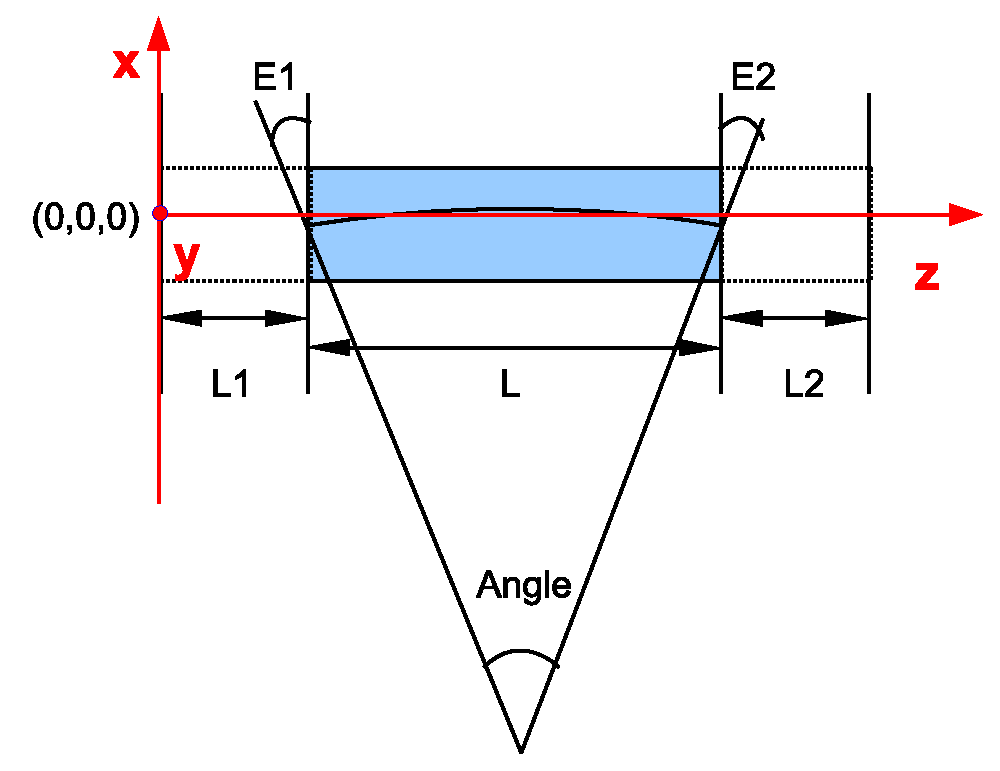
\includegraphics[width=3in,height=2.5in]{ftable-fig1.eps}
  \caption{\label{fig:ftable_mag} Illustration of coordinate
      system and magnet definition.}  
   \end{center} 
\end{figure}

\begin{figure}[htbp] 
  \begin{center}
  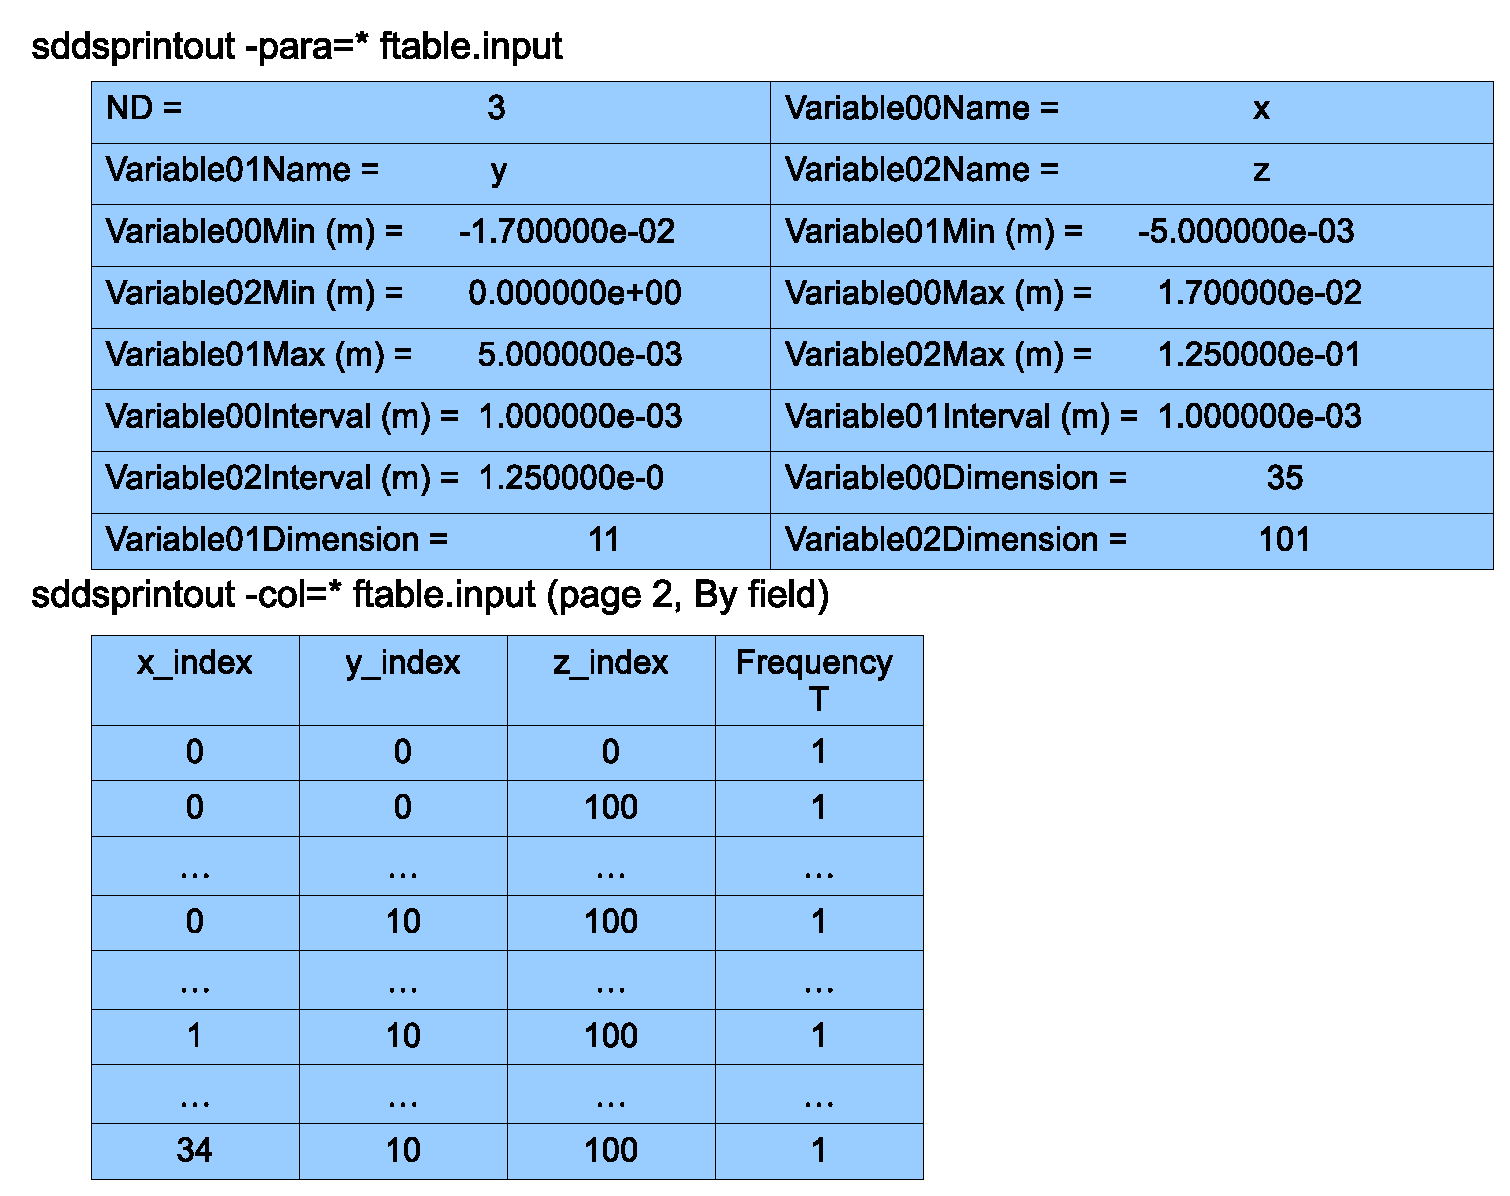
\includegraphics[width=6.5in,height=5.5in]{ftable-fig2.eps}
  \caption{\label{fig:ftable_input} Example of SDDS input
      file. The column x\_index, y\_index, z\_index is not the necessary
      part, it's shown here just for clarifying how the data is
      arranged} 
  \end{center} 
\end{figure}

\newpage
\begin{center}{\Large\verb|FTRFMODE|}\end{center}
\subsection{FTRFMODE---One or more beam-driven TM dipole modes of an RF cavity, with data from a file.}
One or more beam-driven TM dipole modes of an RF cavity, with data from a file.
\\
Parallel capable? : yes\\
GPU capable? : no\\
Back-tracking capable? : no\\
\begin{tabular}{|l|l|l|l|p{\descwidth}|} \hline
Parameter Name & Units & Type & Default & Description \\ \hline 
FILENAME &  & STRING &   NULL            & input file  \\ \hline 
BIN\_SIZE & $S$ & double &  0.0 & bin size for current histogram (use 0 for autosize)  \\ \hline 
N\_BINS &  & long &   20              & number of bins for current histogram  \\ \hline 
RIGID\_UNTIL\_PASS &  & long &  \verb|0| & don't affect the beam until this pass  \\ \hline 
USE\_SYMM\_DATA &  & long &  \verb|0| & use "Symm" columns from URMEL output file?  \\ \hline 
DX & $M$ & double &  0.0 & misalignment  \\ \hline 
DY & $M$ & double &  0.0 & misalignment  \\ \hline 
XFACTOR &  & double &   1 & factor by which to multiply shunt impedances  \\ \hline 
YFACTOR &  & double &   1 & factor by which to multiply shunt impedances  \\ \hline 
CUTOFF & $HZ$ & double &  0.0 & If $>$0, cutoff frequency.  Modes above this frequency are ignored.  \\ \hline 
OUTPUT\_FILE &  & STRING &   NULL            & Output file for voltage in each mode.  \\ \hline 
FLUSH\_INTERVAL &  & long &   1               & Interval in passes at which to flush output data.  \\ \hline 
RAMP\_PASSES &  & long &  \verb|0| & Number of passes over which to linearly ramp up the impedance to full strength.  \\ \hline 
RESET\_FOR\_EACH\_STEP &  & long &   1               & If nonzero, voltage and phase are reset for each simulation step.  \\ \hline 
LONG\_RANGE\_ONLY &  & long &  \verb|0| & If nonzero, induced voltage from present turn does not affect bunch. Short range wake should be included via WAKE or ZLONGIT element.  \\ \hline 
N\_CAVITIES &  & long &   1               & effect is multiplied by this number, simulating N identical cavities  \\ \hline 
\end{tabular}

\newpage
\begin{center}{\Large\verb|FTRFMODE| continued}\end{center}
One or more beam-driven TM dipole modes of an RF cavity, with data from a file.
\\
\begin{tabular}{|l|l|l|l|p{\descwidth}|} \hline
Parameter Name & Units & Type & Default & Description \\ \hline 
BUNCHED\_BEAM\_MODE &  & long &   1               & If non-zero, then do calculations bunch-by-bunch.  \\ \hline 
GROUP &  & string & NULL & Optionally used to assign an element to a group, with a user-defined name.  Group names will appear in the parameter output file in the column ElementGroup  \\ \hline 
\end{tabular}

\vspace*{0.5in}
This element simulates a set of beam-driven dipole modes in a cavity using the fundamental theorem of beam loading and phasor rotation.
It is similar to {\tt TRFMODE}, but it allows faster simulation of more than
one mode.  Also, the mode data is specified in an SDDS file.  This file can be
generated using the APS version of URMEL, or by hand. It must have the following
columns and units:
\begin{enumerate}
\item {\tt Frequency} --- The frequency of the mode in Hz.  Floating point.
\item {\tt Q} --- The quality factor.  Floating point.
\item {\tt ShuntImpedance} or {\tt ShuntImpedanceSymm} --- The shunt
  impedance in Ohms/m, defined as $V^2/(2*P)/x$ or $V^2/(2*P)/y$.
  Floating point. By default, {\tt ShuntImpedance} is used.  However,
  if the parameter \verb|USE_SYMM_DATA| is non-zero, then {\tt
  ShuntImpedanceSymm} is used.  The latter is the full-cavity shunt
  impedance that URMEL computes by assuming that the input cavity used
  is one half of a symmetric cavity.
\end{enumerate}

The file may also have the following columns:
\begin{enumerate}
\item {\tt beta} --- Normalized load impedance (dimensionless).  Floating point. If not given, the
 $\beta=0$ is assumed for all modes. 
\item {\tt xMode} --- If given, then only modes for which the value is nonzero will produce an
 x-plane kick.  Integer.  If not given, all modes affect the x plane.
\item {\tt yMode} --- If given, then only modes for which the value is nonzero will produce an
 y-plane kick.  Integer.  If not given, all modes affect the y plane.
\end{enumerate}
    
{\bf N.B.:} Unlike {\tt TRFMODE}, {\tt FTRFMODE} does not include the longitudinal field that,
strictly speaking, must also be excited.  Generally this is a very small effect.  It will be
added in a future version.

In many simulations, a transient effect may occur when using this
element because, in the context of the simulation, the impedance is
switched on instantaneously.  This can give a false indication of the
threshold for instability. The {\tt RAMP\_PASSES} parameter should
be used to prevent this by slowly ramping the impedance to full
strength.  This idea is from M. Blaskiewicz (BNL).

Normally, the field dumped in the cavity by one particle affects trailing particles in the same turn.
However, if one is also using a \verb|TRWAKE| or \verb|ZTRANSVSE| element to simulate the short-range wake of the cavity, this would be double-counting.
In that case, one can use \verb|LONG_RANGE_ONLY=1| to suppress the same-turn effects of the \verb|RFMODE| element.

\newpage
\begin{center}{\Large\verb|GFWIGGLER|}\end{center}
\subsection{GFWIGGLER---Tracks through a wiggler using generate function method of J. Bahrdt and G. Wuestefeld (BESSY, Berlin, Germany).}
Tracks through a wiggler using generate function method of J. Bahrdt and G. Wuestefeld (BESSY, Berlin, Germany).
\\
Parallel capable? : yes\\
GPU capable? : no\\
Back-tracking capable? : no\\
\begin{tabular}{|l|l|l|l|p{\descwidth}|} \hline
Parameter Name & Units & Type & Default & Description \\ \hline 
L & $M$ & double &  0.0 & Total length  \\ \hline 
B\_MAX & $T$ & double &  0.0 & Maximum on-axis magnetic field at gap=GAP0 and equal longitudinal phases of PHASE\_1,2,3,4  \\ \hline 
SHIM\_SCALE &  & double &   1 & Scaling factor of shim correction field.  \\ \hline 
DX & $M$ & double &  0.0 & Misaligment.  \\ \hline 
DY & $M$ & double &  0.0 & Misaligment.  \\ \hline 
DZ & $M$ & double &  0.0 & Misaligment.  \\ \hline 
TILT & $RAD$ & double &  0.0 & Rotation about beam axis.  \\ \hline 
PERIODS &  & long &  \verb|0| & Total number of wiggler periods. Include end poles  \\ \hline 
STEP &  & long &   1               & Number of normal periods to track for each step  \\ \hline 
ORDER &  & short &  \verb|0| & Order=3 including the 3rd order terms. Otherwise using 2nd order formula.  \\ \hline 
END\_POLE &  & short &   1               & The ending poles are treated as 2 half periods at each sides of the wiggler with reducing field strength, such as 0.25, -0.75, ..., 0.75, -0.25. Periods has to $>$ 2  \\ \hline 
SHIM\_ON &  & short &  \verb|0| & Include shim correction  \\ \hline 
INPUT\_FILE & $ $ & STRING &   NULL            & Name of SDDS file with By harmonic data given at GAP0 and equal longitudinal phases.  \\ \hline 
SHIM\_INPUT & $ $ & STRING &   NULL            & Name of SDDS file with shim field integral harmonic data given at GAP0.  \\ \hline 
SYNCH\_RAD &  & short &  \verb|0| & Include classical, single-particle synchrotron radiation?  \\ \hline 
ISR &  & short &  \verb|0| & Include incoherent synchrotron radiation (quantum excitation)?  \\ \hline 
\end{tabular}

\newpage
\begin{center}{\Large\verb|GFWIGGLER| continued}\end{center}
Tracks through a wiggler using generate function method of J. Bahrdt and G. Wuestefeld (BESSY, Berlin, Germany).
\\
\begin{tabular}{|l|l|l|l|p{\descwidth}|} \hline
Parameter Name & Units & Type & Default & Description \\ \hline 
ISR1PART &  & short &   1               & Include ISR for single-particle beam only if ISR=1 and ISR1PART=1  \\ \hline 
X0 & $M$ & double &  0.0 & Offset of magnet row center in meter.  \\ \hline 
GAP0 & $M$ & double &  0.0 & Nominal magnetic gap.  \\ \hline 
D\_GAP & $M$ & double &  0.0 & Delta gap: actual gap - nominal gap  \\ \hline 
PHASE\_1 & $RAD$ & double &  0.0 & Longitudinal phase of the first row (top right)  \\ \hline 
PHASE\_2 & $RAD$ & double &  0.0 & Longitudinal phase of the second row (top left)  \\ \hline 
PHASE\_3 & $RAD$ & double &  0.0 & Longitudinal phase of the third row (bottom left)  \\ \hline 
PHASE\_4 & $RAD$ & double &  0.0 & Longitudinal phase of the fourth row (bottom right)   \\ \hline 
VERBOSITY &  & short &  \verb|0| & A higher value requires more detailed printouts related to computations.  \\ \hline 
GROUP &  & string & NULL & Optionally used to assign an element to a group, with a user-defined name.  Group names will appear in the parameter output file in the column ElementGroup  \\ \hline 
\end{tabular}

\vspace*{0.5in}
N.B.: at present this element is {\em not} included in computations
of beam moments (\verb|moments_output| command).

This element simulates a wiggler or undulator using the generate
function method given by J. Bahrdt and G. W\"{u}stefeld (``Symplectic
tracking and compensation of dynamic field integrals in complex
undulator structures,'' PRSTAB 14, 040703, 2011.). 

To use the element, one must supply an SDDS file giving harmonic
analysis of the wiggler field. The field expansion used by the code is
for a wiggler working at the nominal gap and provide pure horizontal
deflecting to the on-axis beam. See \verb|CWIGGLER|, horizontal
wiggler with normal poles, for detail explaination of the field
expansion and format of the input file. Besides the required columns
of {\tt Cmn}, {\tt KxOverKw}, {\tt KyOverKw}, and {\tt KzOverKw} by
the \verb|CWIGGLER| elements, two more input columns are needed:
\begin{itemize}
\item The longitudinal harmonic number, $n$, in column {\tt zHarm}.
\item The horizontal harmonic number of $l$, in column {\tt xHarm}.
\end{itemize}
If a file include all required columns from \verb|CWIGGLER| and
\verb|GFWIGGLER| then user can use either of the both methods for
simulating a horizontal planar wiggler.

An universal wiggler field, which be used for generating an arbitrary
polarization, can be derived by given different longitudinal phase
parameters: {\tt PHASE\_1,2,3,4}. The photon energy can be varied by a
non-zero {\tt D\_GAP} value.

\newpage
\begin{center}{\Large\verb|HISTOGRAM|}\end{center}
\subsection{HISTOGRAM---Request for histograms of particle coordinates to be output to SDDS file.}
Request for histograms of particle coordinates to be output to SDDS file.
\\
Parallel capable? : yes\\
GPU capable? : no\\
Back-tracking capable? : yes\\
\begin{tabular}{|l|l|l|l|p{\descwidth}|} \hline
Parameter Name & Units & Type & Default & Description \\ \hline 
FILENAME &  & STRING &                   & filename for histogram output, possibly incomplete (see below)  \\ \hline 
INTERVAL &  & long &   1               & interval in passes between output  \\ \hline 
START\_PASS &  & long &  \verb|0| & starting pass for output  \\ \hline 
BINS &  & long &   50              & number of bins  \\ \hline 
FIXED\_BIN\_SIZE &  & short &  \verb|0| & if nonzero, bin size is fixed after the first histogram is made  \\ \hline 
X\_DATA &  & short &   1               & histogram x and x'?  \\ \hline 
Y\_DATA &  & short &   1               & histogram y and y'?  \\ \hline 
LONGIT\_DATA &  & short &   1               & histogram t and p?  \\ \hline 
BIN\_SIZE\_FACTOR &  & double &   1 & multiply computed bin size by this factor before histogramming  \\ \hline 
NORMALIZE &  & short &   1               & normalize histogram with bin size and number of particles?  \\ \hline 
DISABLE &  & short &  \verb|0| & If nonzero, no output will be generated.  \\ \hline 
SPARSE &  & short &  \verb|0| & If nonzero, only bins with non-zero counts will be output.  \\ \hline 
START\_PID &  & long &   -1              & starting particleID for particles to include  \\ \hline 
END\_PID &  & long &   -1              & ending particleID for particles to include  \\ \hline 
GROUP &  & string & NULL & Optionally used to assign an element to a group, with a user-defined name.  Group names will appear in the parameter output file in the column ElementGroup  \\ \hline 
\end{tabular}

\vspace*{0.5in}
The output filename may be an incomplete filename.  In the case of the
\verb|HISTOGRAM| point element, this means it may contain one instance of
the string format specification ``\%s'' and one occurence of an
integer format specification (e.g., ``\%ld'').  {\tt elegant} will
replace the format with the rootname (see
\verb|run_setup|) and the latter with the element's occurrence
number.  For example, suppose you had a repetitive lattice defined as
follows:
\begin{verbatim}
H1: HISTOGRAM,FILENAME=''%s-%03ld.h1''
Q1: QUAD,L=0.1,K1=1
D: DRIFT,L=1
Q2: QUAD,L=0.1,K1=-1
CELL: LINE=(H1,Q1,D,2*Q2,D,Q1)
BL: LINE=(100*CELL)
\end{verbatim}
The element \verb|H1| appears 100 times.  Each instance will result in
a new file being produced.  Successive instances have names like
``{\em rootname}-001.h1'', ``{\em rootname}-002.h1'', ``{\em
rootname}-003.h1'', and so on up to ``{\em rootname}-100.h1''.  (If
instead of ``\%03ld'' you used ``\%ld'', the names would be ``{\em
rootname}-1.h1'', ``{\em rootname}-2.h1'', etc. up to ``{\em
rootname}-100.h1''.  This is generally not as convenient as the names
don't sort into occurrence order.)

The files can easily be plotted together, as in 
\begin{verbatim}
% sddsplot -column=dt,dtFrequency *-???.h1 -separate 
\end{verbatim}
They may also be combined into a single file, as in
\begin{verbatim}
% sddscombine *-???.h1 all.h1 
\end{verbatim}

In passing, note that if \verb|H1| was defined as
\begin{verbatim}
H1: HISTOGRAM,FILENAME=''%s.h1''
\end{verbatim}
or 
\begin{verbatim}
H1: HISTOGRAM,FILENAME=''output.h1''
\end{verbatim}
only a single file would be produced, containing output from the last instance
only.


\newpage
\begin{center}{\Large\verb|HKICK|}\end{center}
\subsection{HKICK---A horizontal steering dipole implemented as a matrix, up to 2nd order. Use EHKICK for symplectic tracking.}
A horizontal steering dipole implemented as a matrix, up to 2nd order. Use EHKICK for symplectic tracking.
\\
Parallel capable? : yes\\
GPU capable? : yes\\
Back-tracking capable? : no\\
\begin{tabular}{|l|l|l|l|p{\descwidth}|} \hline
Parameter Name & Units & Type & Default & Description \\ \hline 
L & $M$ & double &  0.0 & length  \\ \hline 
KICK & $RAD$ & double &  0.0 & kick strength  \\ \hline 
TILT & $RAD$ & double &  0.0 & rotation about longitudinal axis  \\ \hline 
B2 & $1/M^{2}$ & double &  0.0 & normalized sextupole strength (kick = KICK*(1+B2*x\^2) when y=0)  \\ \hline 
CALIBRATION &  & double &   1 & strength multiplier  \\ \hline 
EDGE\_EFFECTS &  & short &  \verb|0| & include edge effects?  \\ \hline 
ORDER &  & short &  \verb|0| & matrix order  \\ \hline 
STEERING &  & short &   1               & use for steering?  \\ \hline 
SYNCH\_RAD &  & short &  \verb|0| & include classical, single-particle synchrotron radiation?  \\ \hline 
ISR &  & short &  \verb|0| & include incoherent synchrotron radiation (quantum excitation)?  \\ \hline 
LERAD &  & double &  0.0 & if L=0, use this length for radiation computations  \\ \hline 
GROUP &  & string & NULL & Optionally used to assign an element to a group, with a user-defined name.  Group names will appear in the parameter output file in the column ElementGroup  \\ \hline 
\end{tabular}

\newpage
\begin{center}{\Large\verb|HKPOLY|}\end{center}
\subsection{HKPOLY---Applies kick according to a Hamiltonian that's a polynomial function of x and y together with a generalized drift also given as a polynomial of qx and qy}
Applies kick according to a Hamiltonian that's a polynomial function of x and y together with a generalized drift also given as a polynomial of qx and qy
\\
Parallel capable? : yes\\
GPU capable? : no\\
Back-tracking capable? : no\\
\begin{tabular}{|l|l|l|l|p{\descwidth}|} \hline
Parameter Name & Units & Type & Default & Description \\ \hline 
L & $M$ & double &  0.0 & length for geometry only, ignored in tracking  \\ \hline 
K00 &  & double &  0.0 & Coefficient of polynomial for kicks---ignored  \\ \hline 
K01 &  & double &  0.0 & Coefficient of polynomial for kicks  \\ \hline 
K02 &  & double &  0.0 & Coefficient of polynomial for kicks  \\ \hline 
K03 &  & double &  0.0 & Coefficient of polynomial for kicks  \\ \hline 
K04 &  & double &  0.0 & Coefficient of polynomial for kicks  \\ \hline 
K05 &  & double &  0.0 & Coefficient of polynomial for kicks  \\ \hline 
K06 &  & double &  0.0 & Coefficient of polynomial for kicks  \\ \hline 
K10 &  & double &  0.0 & Coefficient of polynomial for kicks  \\ \hline 
K11 &  & double &  0.0 & Coefficient of polynomial for kicks  \\ \hline 
K12 &  & double &  0.0 & Coefficient of polynomial for kicks  \\ \hline 
K13 &  & double &  0.0 & Coefficient of polynomial for kicks  \\ \hline 
K14 &  & double &  0.0 & Coefficient of polynomial for kicks  \\ \hline 
K15 &  & double &  0.0 & Coefficient of polynomial for kicks  \\ \hline 
K16 &  & double &  0.0 & Coefficient of polynomial for kicks  \\ \hline 
K20 &  & double &  0.0 & Coefficient of polynomial for kicks  \\ \hline 
K21 &  & double &  0.0 & Coefficient of polynomial for kicks  \\ \hline 
K22 &  & double &  0.0 & Coefficient of polynomial for kicks  \\ \hline 
\end{tabular}

\newpage
\begin{center}{\Large\verb|HKPOLY| continued}\end{center}
Applies kick according to a Hamiltonian that's a polynomial function of x and y together with a generalized drift also given as a polynomial of qx and qy
\\
\begin{tabular}{|l|l|l|l|p{\descwidth}|} \hline
Parameter Name & Units & Type & Default & Description \\ \hline 
K23 &  & double &  0.0 & Coefficient of polynomial for kicks  \\ \hline 
K24 &  & double &  0.0 & Coefficient of polynomial for kicks  \\ \hline 
K25 &  & double &  0.0 & Coefficient of polynomial for kicks  \\ \hline 
K26 &  & double &  0.0 & Coefficient of polynomial for kicks  \\ \hline 
K30 &  & double &  0.0 & Coefficient of polynomial for kicks  \\ \hline 
K31 &  & double &  0.0 & Coefficient of polynomial for kicks  \\ \hline 
K32 &  & double &  0.0 & Coefficient of polynomial for kicks  \\ \hline 
K33 &  & double &  0.0 & Coefficient of polynomial for kicks  \\ \hline 
K34 &  & double &  0.0 & Coefficient of polynomial for kicks  \\ \hline 
K35 &  & double &  0.0 & Coefficient of polynomial for kicks  \\ \hline 
K36 &  & double &  0.0 & Coefficient of polynomial for kicks  \\ \hline 
K40 &  & double &  0.0 & Coefficient of polynomial for kicks  \\ \hline 
K41 &  & double &  0.0 & Coefficient of polynomial for kicks  \\ \hline 
K42 &  & double &  0.0 & Coefficient of polynomial for kicks  \\ \hline 
K43 &  & double &  0.0 & Coefficient of polynomial for kicks  \\ \hline 
K44 &  & double &  0.0 & Coefficient of polynomial for kicks  \\ \hline 
K45 &  & double &  0.0 & Coefficient of polynomial for kicks  \\ \hline 
K46 &  & double &  0.0 & Coefficient of polynomial for kicks  \\ \hline 
\end{tabular}

\newpage
\begin{center}{\Large\verb|HKPOLY| continued}\end{center}
Applies kick according to a Hamiltonian that's a polynomial function of x and y together with a generalized drift also given as a polynomial of qx and qy
\\
\begin{tabular}{|l|l|l|l|p{\descwidth}|} \hline
Parameter Name & Units & Type & Default & Description \\ \hline 
K50 &  & double &  0.0 & Coefficient of polynomial for kicks  \\ \hline 
K51 &  & double &  0.0 & Coefficient of polynomial for kicks  \\ \hline 
K52 &  & double &  0.0 & Coefficient of polynomial for kicks  \\ \hline 
K53 &  & double &  0.0 & Coefficient of polynomial for kicks  \\ \hline 
K54 &  & double &  0.0 & Coefficient of polynomial for kicks  \\ \hline 
K55 &  & double &  0.0 & Coefficient of polynomial for kicks  \\ \hline 
K56 &  & double &  0.0 & Coefficient of polynomial for kicks  \\ \hline 
K60 &  & double &  0.0 & Coefficient of polynomial for kicks  \\ \hline 
K61 &  & double &  0.0 & Coefficient of polynomial for kicks  \\ \hline 
K62 &  & double &  0.0 & Coefficient of polynomial for kicks  \\ \hline 
K63 &  & double &  0.0 & Coefficient of polynomial for kicks  \\ \hline 
K64 &  & double &  0.0 & Coefficient of polynomial for kicks  \\ \hline 
K65 &  & double &  0.0 & Coefficient of polynomial for kicks  \\ \hline 
K66 &  & double &  0.0 & Coefficient of polynomial for kicks  \\ \hline 
D00 &  & double &  0.0 & Coefficient of polynomial for generalized drift---ignored  \\ \hline 
D01 &  & double &  0.0 & Coefficient of polynomial for generalized drift  \\ \hline 
D02 &  & double &  0.0 & Coefficient of polynomial for generalized drift  \\ \hline 
D03 &  & double &  0.0 & Coefficient of polynomial for generalized drift  \\ \hline 
\end{tabular}

\newpage
\begin{center}{\Large\verb|HKPOLY| continued}\end{center}
Applies kick according to a Hamiltonian that's a polynomial function of x and y together with a generalized drift also given as a polynomial of qx and qy
\\
\begin{tabular}{|l|l|l|l|p{\descwidth}|} \hline
Parameter Name & Units & Type & Default & Description \\ \hline 
D04 &  & double &  0.0 & Coefficient of polynomial for generalized drift  \\ \hline 
D05 &  & double &  0.0 & Coefficient of polynomial for generalized drift  \\ \hline 
D06 &  & double &  0.0 & Coefficient of polynomial for generalized drift  \\ \hline 
D10 &  & double &  0.0 & Coefficient of polynomial for generalized drift  \\ \hline 
D11 &  & double &  0.0 & Coefficient of polynomial for generalized drift  \\ \hline 
D12 &  & double &  0.0 & Coefficient of polynomial for generalized drift  \\ \hline 
D13 &  & double &  0.0 & Coefficient of polynomial for generalized drift  \\ \hline 
D14 &  & double &  0.0 & Coefficient of polynomial for generalized drift  \\ \hline 
D15 &  & double &  0.0 & Coefficient of polynomial for generalized drift  \\ \hline 
D16 &  & double &  0.0 & Coefficient of polynomial for generalized drift  \\ \hline 
D20 &  & double &  0.0 & Coefficient of polynomial for generalized drift  \\ \hline 
D21 &  & double &  0.0 & Coefficient of polynomial for generalized drift  \\ \hline 
D22 &  & double &  0.0 & Coefficient of polynomial for generalized drift  \\ \hline 
D23 &  & double &  0.0 & Coefficient of polynomial for generalized drift  \\ \hline 
D24 &  & double &  0.0 & Coefficient of polynomial for generalized drift  \\ \hline 
D25 &  & double &  0.0 & Coefficient of polynomial for generalized drift  \\ \hline 
D26 &  & double &  0.0 & Coefficient of polynomial for generalized drift  \\ \hline 
D30 &  & double &  0.0 & Coefficient of polynomial for generalized drift  \\ \hline 
\end{tabular}

\newpage
\begin{center}{\Large\verb|HKPOLY| continued}\end{center}
Applies kick according to a Hamiltonian that's a polynomial function of x and y together with a generalized drift also given as a polynomial of qx and qy
\\
\begin{tabular}{|l|l|l|l|p{\descwidth}|} \hline
Parameter Name & Units & Type & Default & Description \\ \hline 
D31 &  & double &  0.0 & Coefficient of polynomial for generalized drift  \\ \hline 
D32 &  & double &  0.0 & Coefficient of polynomial for generalized drift  \\ \hline 
D33 &  & double &  0.0 & Coefficient of polynomial for generalized drift  \\ \hline 
D34 &  & double &  0.0 & Coefficient of polynomial for generalized drift  \\ \hline 
D35 &  & double &  0.0 & Coefficient of polynomial for generalized drift  \\ \hline 
D36 &  & double &  0.0 & Coefficient of polynomial for generalized drift  \\ \hline 
D40 &  & double &  0.0 & Coefficient of polynomial for generalized drift  \\ \hline 
D41 &  & double &  0.0 & Coefficient of polynomial for generalized drift  \\ \hline 
D42 &  & double &  0.0 & Coefficient of polynomial for generalized drift  \\ \hline 
D43 &  & double &  0.0 & Coefficient of polynomial for generalized drift  \\ \hline 
D44 &  & double &  0.0 & Coefficient of polynomial for generalized drift  \\ \hline 
D45 &  & double &  0.0 & Coefficient of polynomial for generalized drift  \\ \hline 
D46 &  & double &  0.0 & Coefficient of polynomial for generalized drift  \\ \hline 
D50 &  & double &  0.0 & Coefficient of polynomial for generalized drift  \\ \hline 
D51 &  & double &  0.0 & Coefficient of polynomial for generalized drift  \\ \hline 
D52 &  & double &  0.0 & Coefficient of polynomial for generalized drift  \\ \hline 
D53 &  & double &  0.0 & Coefficient of polynomial for generalized drift  \\ \hline 
D54 &  & double &  0.0 & Coefficient of polynomial for generalized drift  \\ \hline 
\end{tabular}

\newpage
\begin{center}{\Large\verb|HKPOLY| continued}\end{center}
Applies kick according to a Hamiltonian that's a polynomial function of x and y together with a generalized drift also given as a polynomial of qx and qy
\\
\begin{tabular}{|l|l|l|l|p{\descwidth}|} \hline
Parameter Name & Units & Type & Default & Description \\ \hline 
D55 &  & double &  0.0 & Coefficient of polynomial for generalized drift  \\ \hline 
D56 &  & double &  0.0 & Coefficient of polynomial for generalized drift  \\ \hline 
D60 &  & double &  0.0 & Coefficient of polynomial for generalized drift  \\ \hline 
D61 &  & double &  0.0 & Coefficient of polynomial for generalized drift  \\ \hline 
D62 &  & double &  0.0 & Coefficient of polynomial for generalized drift  \\ \hline 
D63 &  & double &  0.0 & Coefficient of polynomial for generalized drift  \\ \hline 
D64 &  & double &  0.0 & Coefficient of polynomial for generalized drift  \\ \hline 
D65 &  & double &  0.0 & Coefficient of polynomial for generalized drift  \\ \hline 
D66 &  & double &  0.0 & Coefficient of polynomial for generalized drift  \\ \hline 
E000 &  & double &  0.0 & Coefficient of polynomial for type 2 drifts  \\ \hline 
E001 &  & double &  0.0 & Coefficient of polynomial for type 2 drifts  \\ \hline 
E002 &  & double &  0.0 & Coefficient of polynomial for type 2 drifts  \\ \hline 
E003 &  & double &  0.0 & Coefficient of polynomial for type 2 drifts  \\ \hline 
E004 &  & double &  0.0 & Coefficient of polynomial for type 2 drifts  \\ \hline 
E005 &  & double &  0.0 & Coefficient of polynomial for type 2 drifts  \\ \hline 
E006 &  & double &  0.0 & Coefficient of polynomial for type 2 drifts  \\ \hline 
E010 &  & double &  0.0 & Coefficient of polynomial for type 2 drifts  \\ \hline 
E011 &  & double &  0.0 & Coefficient of polynomial for type 2 drifts  \\ \hline 
\end{tabular}

\newpage
\begin{center}{\Large\verb|HKPOLY| continued}\end{center}
Applies kick according to a Hamiltonian that's a polynomial function of x and y together with a generalized drift also given as a polynomial of qx and qy
\\
\begin{tabular}{|l|l|l|l|p{\descwidth}|} \hline
Parameter Name & Units & Type & Default & Description \\ \hline 
E012 &  & double &  0.0 & Coefficient of polynomial for type 2 drifts  \\ \hline 
E013 &  & double &  0.0 & Coefficient of polynomial for type 2 drifts  \\ \hline 
E014 &  & double &  0.0 & Coefficient of polynomial for type 2 drifts  \\ \hline 
E015 &  & double &  0.0 & Coefficient of polynomial for type 2 drifts  \\ \hline 
E016 &  & double &  0.0 & Coefficient of polynomial for type 2 drifts  \\ \hline 
E020 &  & double &  0.0 & Coefficient of polynomial for type 2 drifts  \\ \hline 
E021 &  & double &  0.0 & Coefficient of polynomial for type 2 drifts  \\ \hline 
E022 &  & double &  0.0 & Coefficient of polynomial for type 2 drifts  \\ \hline 
E023 &  & double &  0.0 & Coefficient of polynomial for type 2 drifts  \\ \hline 
E024 &  & double &  0.0 & Coefficient of polynomial for type 2 drifts  \\ \hline 
E025 &  & double &  0.0 & Coefficient of polynomial for type 2 drifts  \\ \hline 
E026 &  & double &  0.0 & Coefficient of polynomial for type 2 drifts  \\ \hline 
E030 &  & double &  0.0 & Coefficient of polynomial for type 2 drifts  \\ \hline 
E031 &  & double &  0.0 & Coefficient of polynomial for type 2 drifts  \\ \hline 
E032 &  & double &  0.0 & Coefficient of polynomial for type 2 drifts  \\ \hline 
E033 &  & double &  0.0 & Coefficient of polynomial for type 2 drifts  \\ \hline 
E034 &  & double &  0.0 & Coefficient of polynomial for type 2 drifts  \\ \hline 
E035 &  & double &  0.0 & Coefficient of polynomial for type 2 drifts  \\ \hline 
\end{tabular}

\newpage
\begin{center}{\Large\verb|HKPOLY| continued}\end{center}
Applies kick according to a Hamiltonian that's a polynomial function of x and y together with a generalized drift also given as a polynomial of qx and qy
\\
\begin{tabular}{|l|l|l|l|p{\descwidth}|} \hline
Parameter Name & Units & Type & Default & Description \\ \hline 
E036 &  & double &  0.0 & Coefficient of polynomial for type 2 drifts  \\ \hline 
E040 &  & double &  0.0 & Coefficient of polynomial for type 2 drifts  \\ \hline 
E041 &  & double &  0.0 & Coefficient of polynomial for type 2 drifts  \\ \hline 
E042 &  & double &  0.0 & Coefficient of polynomial for type 2 drifts  \\ \hline 
E043 &  & double &  0.0 & Coefficient of polynomial for type 2 drifts  \\ \hline 
E044 &  & double &  0.0 & Coefficient of polynomial for type 2 drifts  \\ \hline 
E045 &  & double &  0.0 & Coefficient of polynomial for type 2 drifts  \\ \hline 
E046 &  & double &  0.0 & Coefficient of polynomial for type 2 drifts  \\ \hline 
E050 &  & double &  0.0 & Coefficient of polynomial for type 2 drifts  \\ \hline 
E051 &  & double &  0.0 & Coefficient of polynomial for type 2 drifts  \\ \hline 
E052 &  & double &  0.0 & Coefficient of polynomial for type 2 drifts  \\ \hline 
E053 &  & double &  0.0 & Coefficient of polynomial for type 2 drifts  \\ \hline 
E054 &  & double &  0.0 & Coefficient of polynomial for type 2 drifts  \\ \hline 
E055 &  & double &  0.0 & Coefficient of polynomial for type 2 drifts  \\ \hline 
E056 &  & double &  0.0 & Coefficient of polynomial for type 2 drifts  \\ \hline 
E060 &  & double &  0.0 & Coefficient of polynomial for type 2 drifts  \\ \hline 
E061 &  & double &  0.0 & Coefficient of polynomial for type 2 drifts  \\ \hline 
E062 &  & double &  0.0 & Coefficient of polynomial for type 2 drifts  \\ \hline 
\end{tabular}

\newpage
\begin{center}{\Large\verb|HKPOLY| continued}\end{center}
Applies kick according to a Hamiltonian that's a polynomial function of x and y together with a generalized drift also given as a polynomial of qx and qy
\\
\begin{tabular}{|l|l|l|l|p{\descwidth}|} \hline
Parameter Name & Units & Type & Default & Description \\ \hline 
E063 &  & double &  0.0 & Coefficient of polynomial for type 2 drifts  \\ \hline 
E064 &  & double &  0.0 & Coefficient of polynomial for type 2 drifts  \\ \hline 
E065 &  & double &  0.0 & Coefficient of polynomial for type 2 drifts  \\ \hline 
E066 &  & double &  0.0 & Coefficient of polynomial for type 2 drifts  \\ \hline 
E100 &  & double &  0.0 & Coefficient of polynomial for type 2 drifts  \\ \hline 
E101 &  & double &  0.0 & Coefficient of polynomial for type 2 drifts  \\ \hline 
E102 &  & double &  0.0 & Coefficient of polynomial for type 2 drifts  \\ \hline 
E103 &  & double &  0.0 & Coefficient of polynomial for type 2 drifts  \\ \hline 
E104 &  & double &  0.0 & Coefficient of polynomial for type 2 drifts  \\ \hline 
E105 &  & double &  0.0 & Coefficient of polynomial for type 2 drifts  \\ \hline 
E106 &  & double &  0.0 & Coefficient of polynomial for type 2 drifts  \\ \hline 
E110 &  & double &  0.0 & Coefficient of polynomial for type 2 drifts  \\ \hline 
E111 &  & double &  0.0 & Coefficient of polynomial for type 2 drifts  \\ \hline 
E112 &  & double &  0.0 & Coefficient of polynomial for type 2 drifts  \\ \hline 
E113 &  & double &  0.0 & Coefficient of polynomial for type 2 drifts  \\ \hline 
E114 &  & double &  0.0 & Coefficient of polynomial for type 2 drifts  \\ \hline 
E115 &  & double &  0.0 & Coefficient of polynomial for type 2 drifts  \\ \hline 
E116 &  & double &  0.0 & Coefficient of polynomial for type 2 drifts  \\ \hline 
\end{tabular}

\newpage
\begin{center}{\Large\verb|HKPOLY| continued}\end{center}
Applies kick according to a Hamiltonian that's a polynomial function of x and y together with a generalized drift also given as a polynomial of qx and qy
\\
\begin{tabular}{|l|l|l|l|p{\descwidth}|} \hline
Parameter Name & Units & Type & Default & Description \\ \hline 
E120 &  & double &  0.0 & Coefficient of polynomial for type 2 drifts  \\ \hline 
E121 &  & double &  0.0 & Coefficient of polynomial for type 2 drifts  \\ \hline 
E122 &  & double &  0.0 & Coefficient of polynomial for type 2 drifts  \\ \hline 
E123 &  & double &  0.0 & Coefficient of polynomial for type 2 drifts  \\ \hline 
E124 &  & double &  0.0 & Coefficient of polynomial for type 2 drifts  \\ \hline 
E125 &  & double &  0.0 & Coefficient of polynomial for type 2 drifts  \\ \hline 
E126 &  & double &  0.0 & Coefficient of polynomial for type 2 drifts  \\ \hline 
E130 &  & double &  0.0 & Coefficient of polynomial for type 2 drifts  \\ \hline 
E131 &  & double &  0.0 & Coefficient of polynomial for type 2 drifts  \\ \hline 
E132 &  & double &  0.0 & Coefficient of polynomial for type 2 drifts  \\ \hline 
E133 &  & double &  0.0 & Coefficient of polynomial for type 2 drifts  \\ \hline 
E134 &  & double &  0.0 & Coefficient of polynomial for type 2 drifts  \\ \hline 
E135 &  & double &  0.0 & Coefficient of polynomial for type 2 drifts  \\ \hline 
E136 &  & double &  0.0 & Coefficient of polynomial for type 2 drifts  \\ \hline 
E140 &  & double &  0.0 & Coefficient of polynomial for type 2 drifts  \\ \hline 
E141 &  & double &  0.0 & Coefficient of polynomial for type 2 drifts  \\ \hline 
E142 &  & double &  0.0 & Coefficient of polynomial for type 2 drifts  \\ \hline 
E143 &  & double &  0.0 & Coefficient of polynomial for type 2 drifts  \\ \hline 
\end{tabular}

\newpage
\begin{center}{\Large\verb|HKPOLY| continued}\end{center}
Applies kick according to a Hamiltonian that's a polynomial function of x and y together with a generalized drift also given as a polynomial of qx and qy
\\
\begin{tabular}{|l|l|l|l|p{\descwidth}|} \hline
Parameter Name & Units & Type & Default & Description \\ \hline 
E144 &  & double &  0.0 & Coefficient of polynomial for type 2 drifts  \\ \hline 
E145 &  & double &  0.0 & Coefficient of polynomial for type 2 drifts  \\ \hline 
E146 &  & double &  0.0 & Coefficient of polynomial for type 2 drifts  \\ \hline 
E150 &  & double &  0.0 & Coefficient of polynomial for type 2 drifts  \\ \hline 
E151 &  & double &  0.0 & Coefficient of polynomial for type 2 drifts  \\ \hline 
E152 &  & double &  0.0 & Coefficient of polynomial for type 2 drifts  \\ \hline 
E153 &  & double &  0.0 & Coefficient of polynomial for type 2 drifts  \\ \hline 
E154 &  & double &  0.0 & Coefficient of polynomial for type 2 drifts  \\ \hline 
E155 &  & double &  0.0 & Coefficient of polynomial for type 2 drifts  \\ \hline 
E156 &  & double &  0.0 & Coefficient of polynomial for type 2 drifts  \\ \hline 
E160 &  & double &  0.0 & Coefficient of polynomial for type 2 drifts  \\ \hline 
E161 &  & double &  0.0 & Coefficient of polynomial for type 2 drifts  \\ \hline 
E162 &  & double &  0.0 & Coefficient of polynomial for type 2 drifts  \\ \hline 
E163 &  & double &  0.0 & Coefficient of polynomial for type 2 drifts  \\ \hline 
E164 &  & double &  0.0 & Coefficient of polynomial for type 2 drifts  \\ \hline 
E165 &  & double &  0.0 & Coefficient of polynomial for type 2 drifts  \\ \hline 
E166 &  & double &  0.0 & Coefficient of polynomial for type 2 drifts  \\ \hline 
E200 &  & double &  0.0 & Coefficient of polynomial for type 2 drifts  \\ \hline 
\end{tabular}

\newpage
\begin{center}{\Large\verb|HKPOLY| continued}\end{center}
Applies kick according to a Hamiltonian that's a polynomial function of x and y together with a generalized drift also given as a polynomial of qx and qy
\\
\begin{tabular}{|l|l|l|l|p{\descwidth}|} \hline
Parameter Name & Units & Type & Default & Description \\ \hline 
E201 &  & double &  0.0 & Coefficient of polynomial for type 2 drifts  \\ \hline 
E202 &  & double &  0.0 & Coefficient of polynomial for type 2 drifts  \\ \hline 
E203 &  & double &  0.0 & Coefficient of polynomial for type 2 drifts  \\ \hline 
E204 &  & double &  0.0 & Coefficient of polynomial for type 2 drifts  \\ \hline 
E205 &  & double &  0.0 & Coefficient of polynomial for type 2 drifts  \\ \hline 
E206 &  & double &  0.0 & Coefficient of polynomial for type 2 drifts  \\ \hline 
E210 &  & double &  0.0 & Coefficient of polynomial for type 2 drifts  \\ \hline 
E211 &  & double &  0.0 & Coefficient of polynomial for type 2 drifts  \\ \hline 
E212 &  & double &  0.0 & Coefficient of polynomial for type 2 drifts  \\ \hline 
E213 &  & double &  0.0 & Coefficient of polynomial for type 2 drifts  \\ \hline 
E214 &  & double &  0.0 & Coefficient of polynomial for type 2 drifts  \\ \hline 
E215 &  & double &  0.0 & Coefficient of polynomial for type 2 drifts  \\ \hline 
E216 &  & double &  0.0 & Coefficient of polynomial for type 2 drifts  \\ \hline 
E220 &  & double &  0.0 & Coefficient of polynomial for type 2 drifts  \\ \hline 
E221 &  & double &  0.0 & Coefficient of polynomial for type 2 drifts  \\ \hline 
E222 &  & double &  0.0 & Coefficient of polynomial for type 2 drifts  \\ \hline 
E223 &  & double &  0.0 & Coefficient of polynomial for type 2 drifts  \\ \hline 
E224 &  & double &  0.0 & Coefficient of polynomial for type 2 drifts  \\ \hline 
\end{tabular}

\newpage
\begin{center}{\Large\verb|HKPOLY| continued}\end{center}
Applies kick according to a Hamiltonian that's a polynomial function of x and y together with a generalized drift also given as a polynomial of qx and qy
\\
\begin{tabular}{|l|l|l|l|p{\descwidth}|} \hline
Parameter Name & Units & Type & Default & Description \\ \hline 
E225 &  & double &  0.0 & Coefficient of polynomial for type 2 drifts  \\ \hline 
E226 &  & double &  0.0 & Coefficient of polynomial for type 2 drifts  \\ \hline 
E230 &  & double &  0.0 & Coefficient of polynomial for type 2 drifts  \\ \hline 
E231 &  & double &  0.0 & Coefficient of polynomial for type 2 drifts  \\ \hline 
E232 &  & double &  0.0 & Coefficient of polynomial for type 2 drifts  \\ \hline 
E233 &  & double &  0.0 & Coefficient of polynomial for type 2 drifts  \\ \hline 
E234 &  & double &  0.0 & Coefficient of polynomial for type 2 drifts  \\ \hline 
E235 &  & double &  0.0 & Coefficient of polynomial for type 2 drifts  \\ \hline 
E236 &  & double &  0.0 & Coefficient of polynomial for type 2 drifts  \\ \hline 
E240 &  & double &  0.0 & Coefficient of polynomial for type 2 drifts  \\ \hline 
E241 &  & double &  0.0 & Coefficient of polynomial for type 2 drifts  \\ \hline 
E242 &  & double &  0.0 & Coefficient of polynomial for type 2 drifts  \\ \hline 
E243 &  & double &  0.0 & Coefficient of polynomial for type 2 drifts  \\ \hline 
E244 &  & double &  0.0 & Coefficient of polynomial for type 2 drifts  \\ \hline 
E245 &  & double &  0.0 & Coefficient of polynomial for type 2 drifts  \\ \hline 
E246 &  & double &  0.0 & Coefficient of polynomial for type 2 drifts  \\ \hline 
E250 &  & double &  0.0 & Coefficient of polynomial for type 2 drifts  \\ \hline 
E251 &  & double &  0.0 & Coefficient of polynomial for type 2 drifts  \\ \hline 
\end{tabular}

\newpage
\begin{center}{\Large\verb|HKPOLY| continued}\end{center}
Applies kick according to a Hamiltonian that's a polynomial function of x and y together with a generalized drift also given as a polynomial of qx and qy
\\
\begin{tabular}{|l|l|l|l|p{\descwidth}|} \hline
Parameter Name & Units & Type & Default & Description \\ \hline 
E252 &  & double &  0.0 & Coefficient of polynomial for type 2 drifts  \\ \hline 
E253 &  & double &  0.0 & Coefficient of polynomial for type 2 drifts  \\ \hline 
E254 &  & double &  0.0 & Coefficient of polynomial for type 2 drifts  \\ \hline 
E255 &  & double &  0.0 & Coefficient of polynomial for type 2 drifts  \\ \hline 
E256 &  & double &  0.0 & Coefficient of polynomial for type 2 drifts  \\ \hline 
E260 &  & double &  0.0 & Coefficient of polynomial for type 2 drifts  \\ \hline 
E261 &  & double &  0.0 & Coefficient of polynomial for type 2 drifts  \\ \hline 
E262 &  & double &  0.0 & Coefficient of polynomial for type 2 drifts  \\ \hline 
E263 &  & double &  0.0 & Coefficient of polynomial for type 2 drifts  \\ \hline 
E264 &  & double &  0.0 & Coefficient of polynomial for type 2 drifts  \\ \hline 
E265 &  & double &  0.0 & Coefficient of polynomial for type 2 drifts  \\ \hline 
E266 &  & double &  0.0 & Coefficient of polynomial for type 2 drifts  \\ \hline 
E300 &  & double &  0.0 & Coefficient of polynomial for type 2 drifts  \\ \hline 
E301 &  & double &  0.0 & Coefficient of polynomial for type 2 drifts  \\ \hline 
E302 &  & double &  0.0 & Coefficient of polynomial for type 2 drifts  \\ \hline 
E303 &  & double &  0.0 & Coefficient of polynomial for type 2 drifts  \\ \hline 
E304 &  & double &  0.0 & Coefficient of polynomial for type 2 drifts  \\ \hline 
E305 &  & double &  0.0 & Coefficient of polynomial for type 2 drifts  \\ \hline 
\end{tabular}

\newpage
\begin{center}{\Large\verb|HKPOLY| continued}\end{center}
Applies kick according to a Hamiltonian that's a polynomial function of x and y together with a generalized drift also given as a polynomial of qx and qy
\\
\begin{tabular}{|l|l|l|l|p{\descwidth}|} \hline
Parameter Name & Units & Type & Default & Description \\ \hline 
E306 &  & double &  0.0 & Coefficient of polynomial for type 2 drifts  \\ \hline 
E310 &  & double &  0.0 & Coefficient of polynomial for type 2 drifts  \\ \hline 
E311 &  & double &  0.0 & Coefficient of polynomial for type 2 drifts  \\ \hline 
E312 &  & double &  0.0 & Coefficient of polynomial for type 2 drifts  \\ \hline 
E313 &  & double &  0.0 & Coefficient of polynomial for type 2 drifts  \\ \hline 
E314 &  & double &  0.0 & Coefficient of polynomial for type 2 drifts  \\ \hline 
E315 &  & double &  0.0 & Coefficient of polynomial for type 2 drifts  \\ \hline 
E316 &  & double &  0.0 & Coefficient of polynomial for type 2 drifts  \\ \hline 
E320 &  & double &  0.0 & Coefficient of polynomial for type 2 drifts  \\ \hline 
E321 &  & double &  0.0 & Coefficient of polynomial for type 2 drifts  \\ \hline 
E322 &  & double &  0.0 & Coefficient of polynomial for type 2 drifts  \\ \hline 
E323 &  & double &  0.0 & Coefficient of polynomial for type 2 drifts  \\ \hline 
E324 &  & double &  0.0 & Coefficient of polynomial for type 2 drifts  \\ \hline 
E325 &  & double &  0.0 & Coefficient of polynomial for type 2 drifts  \\ \hline 
E326 &  & double &  0.0 & Coefficient of polynomial for type 2 drifts  \\ \hline 
E330 &  & double &  0.0 & Coefficient of polynomial for type 2 drifts  \\ \hline 
E331 &  & double &  0.0 & Coefficient of polynomial for type 2 drifts  \\ \hline 
E332 &  & double &  0.0 & Coefficient of polynomial for type 2 drifts  \\ \hline 
\end{tabular}

\newpage
\begin{center}{\Large\verb|HKPOLY| continued}\end{center}
Applies kick according to a Hamiltonian that's a polynomial function of x and y together with a generalized drift also given as a polynomial of qx and qy
\\
\begin{tabular}{|l|l|l|l|p{\descwidth}|} \hline
Parameter Name & Units & Type & Default & Description \\ \hline 
E333 &  & double &  0.0 & Coefficient of polynomial for type 2 drifts  \\ \hline 
E334 &  & double &  0.0 & Coefficient of polynomial for type 2 drifts  \\ \hline 
E335 &  & double &  0.0 & Coefficient of polynomial for type 2 drifts  \\ \hline 
E336 &  & double &  0.0 & Coefficient of polynomial for type 2 drifts  \\ \hline 
E340 &  & double &  0.0 & Coefficient of polynomial for type 2 drifts  \\ \hline 
E341 &  & double &  0.0 & Coefficient of polynomial for type 2 drifts  \\ \hline 
E342 &  & double &  0.0 & Coefficient of polynomial for type 2 drifts  \\ \hline 
E343 &  & double &  0.0 & Coefficient of polynomial for type 2 drifts  \\ \hline 
E344 &  & double &  0.0 & Coefficient of polynomial for type 2 drifts  \\ \hline 
E345 &  & double &  0.0 & Coefficient of polynomial for type 2 drifts  \\ \hline 
E346 &  & double &  0.0 & Coefficient of polynomial for type 2 drifts  \\ \hline 
E350 &  & double &  0.0 & Coefficient of polynomial for type 2 drifts  \\ \hline 
E351 &  & double &  0.0 & Coefficient of polynomial for type 2 drifts  \\ \hline 
E352 &  & double &  0.0 & Coefficient of polynomial for type 2 drifts  \\ \hline 
E353 &  & double &  0.0 & Coefficient of polynomial for type 2 drifts  \\ \hline 
E354 &  & double &  0.0 & Coefficient of polynomial for type 2 drifts  \\ \hline 
E355 &  & double &  0.0 & Coefficient of polynomial for type 2 drifts  \\ \hline 
E356 &  & double &  0.0 & Coefficient of polynomial for type 2 drifts  \\ \hline 
\end{tabular}

\newpage
\begin{center}{\Large\verb|HKPOLY| continued}\end{center}
Applies kick according to a Hamiltonian that's a polynomial function of x and y together with a generalized drift also given as a polynomial of qx and qy
\\
\begin{tabular}{|l|l|l|l|p{\descwidth}|} \hline
Parameter Name & Units & Type & Default & Description \\ \hline 
E360 &  & double &  0.0 & Coefficient of polynomial for type 2 drifts  \\ \hline 
E361 &  & double &  0.0 & Coefficient of polynomial for type 2 drifts  \\ \hline 
E362 &  & double &  0.0 & Coefficient of polynomial for type 2 drifts  \\ \hline 
E363 &  & double &  0.0 & Coefficient of polynomial for type 2 drifts  \\ \hline 
E364 &  & double &  0.0 & Coefficient of polynomial for type 2 drifts  \\ \hline 
E365 &  & double &  0.0 & Coefficient of polynomial for type 2 drifts  \\ \hline 
E366 &  & double &  0.0 & Coefficient of polynomial for type 2 drifts  \\ \hline 
E400 &  & double &  0.0 & Coefficient of polynomial for type 2 drifts  \\ \hline 
E401 &  & double &  0.0 & Coefficient of polynomial for type 2 drifts  \\ \hline 
E402 &  & double &  0.0 & Coefficient of polynomial for type 2 drifts  \\ \hline 
E403 &  & double &  0.0 & Coefficient of polynomial for type 2 drifts  \\ \hline 
E404 &  & double &  0.0 & Coefficient of polynomial for type 2 drifts  \\ \hline 
E405 &  & double &  0.0 & Coefficient of polynomial for type 2 drifts  \\ \hline 
E406 &  & double &  0.0 & Coefficient of polynomial for type 2 drifts  \\ \hline 
E410 &  & double &  0.0 & Coefficient of polynomial for type 2 drifts  \\ \hline 
E411 &  & double &  0.0 & Coefficient of polynomial for type 2 drifts  \\ \hline 
E412 &  & double &  0.0 & Coefficient of polynomial for type 2 drifts  \\ \hline 
E413 &  & double &  0.0 & Coefficient of polynomial for type 2 drifts  \\ \hline 
\end{tabular}

\newpage
\begin{center}{\Large\verb|HKPOLY| continued}\end{center}
Applies kick according to a Hamiltonian that's a polynomial function of x and y together with a generalized drift also given as a polynomial of qx and qy
\\
\begin{tabular}{|l|l|l|l|p{\descwidth}|} \hline
Parameter Name & Units & Type & Default & Description \\ \hline 
E414 &  & double &  0.0 & Coefficient of polynomial for type 2 drifts  \\ \hline 
E415 &  & double &  0.0 & Coefficient of polynomial for type 2 drifts  \\ \hline 
E416 &  & double &  0.0 & Coefficient of polynomial for type 2 drifts  \\ \hline 
E420 &  & double &  0.0 & Coefficient of polynomial for type 2 drifts  \\ \hline 
E421 &  & double &  0.0 & Coefficient of polynomial for type 2 drifts  \\ \hline 
E422 &  & double &  0.0 & Coefficient of polynomial for type 2 drifts  \\ \hline 
E423 &  & double &  0.0 & Coefficient of polynomial for type 2 drifts  \\ \hline 
E424 &  & double &  0.0 & Coefficient of polynomial for type 2 drifts  \\ \hline 
E425 &  & double &  0.0 & Coefficient of polynomial for type 2 drifts  \\ \hline 
E426 &  & double &  0.0 & Coefficient of polynomial for type 2 drifts  \\ \hline 
E430 &  & double &  0.0 & Coefficient of polynomial for type 2 drifts  \\ \hline 
E431 &  & double &  0.0 & Coefficient of polynomial for type 2 drifts  \\ \hline 
E432 &  & double &  0.0 & Coefficient of polynomial for type 2 drifts  \\ \hline 
E433 &  & double &  0.0 & Coefficient of polynomial for type 2 drifts  \\ \hline 
E434 &  & double &  0.0 & Coefficient of polynomial for type 2 drifts  \\ \hline 
E435 &  & double &  0.0 & Coefficient of polynomial for type 2 drifts  \\ \hline 
E436 &  & double &  0.0 & Coefficient of polynomial for type 2 drifts  \\ \hline 
E440 &  & double &  0.0 & Coefficient of polynomial for type 2 drifts  \\ \hline 
\end{tabular}

\newpage
\begin{center}{\Large\verb|HKPOLY| continued}\end{center}
Applies kick according to a Hamiltonian that's a polynomial function of x and y together with a generalized drift also given as a polynomial of qx and qy
\\
\begin{tabular}{|l|l|l|l|p{\descwidth}|} \hline
Parameter Name & Units & Type & Default & Description \\ \hline 
E441 &  & double &  0.0 & Coefficient of polynomial for type 2 drifts  \\ \hline 
E442 &  & double &  0.0 & Coefficient of polynomial for type 2 drifts  \\ \hline 
E443 &  & double &  0.0 & Coefficient of polynomial for type 2 drifts  \\ \hline 
E444 &  & double &  0.0 & Coefficient of polynomial for type 2 drifts  \\ \hline 
E445 &  & double &  0.0 & Coefficient of polynomial for type 2 drifts  \\ \hline 
E446 &  & double &  0.0 & Coefficient of polynomial for type 2 drifts  \\ \hline 
E450 &  & double &  0.0 & Coefficient of polynomial for type 2 drifts  \\ \hline 
E451 &  & double &  0.0 & Coefficient of polynomial for type 2 drifts  \\ \hline 
E452 &  & double &  0.0 & Coefficient of polynomial for type 2 drifts  \\ \hline 
E453 &  & double &  0.0 & Coefficient of polynomial for type 2 drifts  \\ \hline 
E454 &  & double &  0.0 & Coefficient of polynomial for type 2 drifts  \\ \hline 
E455 &  & double &  0.0 & Coefficient of polynomial for type 2 drifts  \\ \hline 
E456 &  & double &  0.0 & Coefficient of polynomial for type 2 drifts  \\ \hline 
E460 &  & double &  0.0 & Coefficient of polynomial for type 2 drifts  \\ \hline 
E461 &  & double &  0.0 & Coefficient of polynomial for type 2 drifts  \\ \hline 
E462 &  & double &  0.0 & Coefficient of polynomial for type 2 drifts  \\ \hline 
E463 &  & double &  0.0 & Coefficient of polynomial for type 2 drifts  \\ \hline 
E464 &  & double &  0.0 & Coefficient of polynomial for type 2 drifts  \\ \hline 
\end{tabular}

\newpage
\begin{center}{\Large\verb|HKPOLY| continued}\end{center}
Applies kick according to a Hamiltonian that's a polynomial function of x and y together with a generalized drift also given as a polynomial of qx and qy
\\
\begin{tabular}{|l|l|l|l|p{\descwidth}|} \hline
Parameter Name & Units & Type & Default & Description \\ \hline 
E465 &  & double &  0.0 & Coefficient of polynomial for type 2 drifts  \\ \hline 
E466 &  & double &  0.0 & Coefficient of polynomial for type 2 drifts  \\ \hline 
E500 &  & double &  0.0 & Coefficient of polynomial for type 2 drifts  \\ \hline 
E501 &  & double &  0.0 & Coefficient of polynomial for type 2 drifts  \\ \hline 
E502 &  & double &  0.0 & Coefficient of polynomial for type 2 drifts  \\ \hline 
E503 &  & double &  0.0 & Coefficient of polynomial for type 2 drifts  \\ \hline 
E504 &  & double &  0.0 & Coefficient of polynomial for type 2 drifts  \\ \hline 
E505 &  & double &  0.0 & Coefficient of polynomial for type 2 drifts  \\ \hline 
E506 &  & double &  0.0 & Coefficient of polynomial for type 2 drifts  \\ \hline 
E510 &  & double &  0.0 & Coefficient of polynomial for type 2 drifts  \\ \hline 
E511 &  & double &  0.0 & Coefficient of polynomial for type 2 drifts  \\ \hline 
E512 &  & double &  0.0 & Coefficient of polynomial for type 2 drifts  \\ \hline 
E513 &  & double &  0.0 & Coefficient of polynomial for type 2 drifts  \\ \hline 
E514 &  & double &  0.0 & Coefficient of polynomial for type 2 drifts  \\ \hline 
E515 &  & double &  0.0 & Coefficient of polynomial for type 2 drifts  \\ \hline 
E516 &  & double &  0.0 & Coefficient of polynomial for type 2 drifts  \\ \hline 
E520 &  & double &  0.0 & Coefficient of polynomial for type 2 drifts  \\ \hline 
E521 &  & double &  0.0 & Coefficient of polynomial for type 2 drifts  \\ \hline 
\end{tabular}

\newpage
\begin{center}{\Large\verb|HKPOLY| continued}\end{center}
Applies kick according to a Hamiltonian that's a polynomial function of x and y together with a generalized drift also given as a polynomial of qx and qy
\\
\begin{tabular}{|l|l|l|l|p{\descwidth}|} \hline
Parameter Name & Units & Type & Default & Description \\ \hline 
E522 &  & double &  0.0 & Coefficient of polynomial for type 2 drifts  \\ \hline 
E523 &  & double &  0.0 & Coefficient of polynomial for type 2 drifts  \\ \hline 
E524 &  & double &  0.0 & Coefficient of polynomial for type 2 drifts  \\ \hline 
E525 &  & double &  0.0 & Coefficient of polynomial for type 2 drifts  \\ \hline 
E526 &  & double &  0.0 & Coefficient of polynomial for type 2 drifts  \\ \hline 
E530 &  & double &  0.0 & Coefficient of polynomial for type 2 drifts  \\ \hline 
E531 &  & double &  0.0 & Coefficient of polynomial for type 2 drifts  \\ \hline 
E532 &  & double &  0.0 & Coefficient of polynomial for type 2 drifts  \\ \hline 
E533 &  & double &  0.0 & Coefficient of polynomial for type 2 drifts  \\ \hline 
E534 &  & double &  0.0 & Coefficient of polynomial for type 2 drifts  \\ \hline 
E535 &  & double &  0.0 & Coefficient of polynomial for type 2 drifts  \\ \hline 
E536 &  & double &  0.0 & Coefficient of polynomial for type 2 drifts  \\ \hline 
E540 &  & double &  0.0 & Coefficient of polynomial for type 2 drifts  \\ \hline 
E541 &  & double &  0.0 & Coefficient of polynomial for type 2 drifts  \\ \hline 
E542 &  & double &  0.0 & Coefficient of polynomial for type 2 drifts  \\ \hline 
E543 &  & double &  0.0 & Coefficient of polynomial for type 2 drifts  \\ \hline 
E544 &  & double &  0.0 & Coefficient of polynomial for type 2 drifts  \\ \hline 
E545 &  & double &  0.0 & Coefficient of polynomial for type 2 drifts  \\ \hline 
\end{tabular}

\newpage
\begin{center}{\Large\verb|HKPOLY| continued}\end{center}
Applies kick according to a Hamiltonian that's a polynomial function of x and y together with a generalized drift also given as a polynomial of qx and qy
\\
\begin{tabular}{|l|l|l|l|p{\descwidth}|} \hline
Parameter Name & Units & Type & Default & Description \\ \hline 
E546 &  & double &  0.0 & Coefficient of polynomial for type 2 drifts  \\ \hline 
E550 &  & double &  0.0 & Coefficient of polynomial for type 2 drifts  \\ \hline 
E551 &  & double &  0.0 & Coefficient of polynomial for type 2 drifts  \\ \hline 
E552 &  & double &  0.0 & Coefficient of polynomial for type 2 drifts  \\ \hline 
E553 &  & double &  0.0 & Coefficient of polynomial for type 2 drifts  \\ \hline 
E554 &  & double &  0.0 & Coefficient of polynomial for type 2 drifts  \\ \hline 
E555 &  & double &  0.0 & Coefficient of polynomial for type 2 drifts  \\ \hline 
E556 &  & double &  0.0 & Coefficient of polynomial for type 2 drifts  \\ \hline 
E560 &  & double &  0.0 & Coefficient of polynomial for type 2 drifts  \\ \hline 
E561 &  & double &  0.0 & Coefficient of polynomial for type 2 drifts  \\ \hline 
E562 &  & double &  0.0 & Coefficient of polynomial for type 2 drifts  \\ \hline 
E563 &  & double &  0.0 & Coefficient of polynomial for type 2 drifts  \\ \hline 
E564 &  & double &  0.0 & Coefficient of polynomial for type 2 drifts  \\ \hline 
E565 &  & double &  0.0 & Coefficient of polynomial for type 2 drifts  \\ \hline 
E566 &  & double &  0.0 & Coefficient of polynomial for type 2 drifts  \\ \hline 
E600 &  & double &  0.0 & Coefficient of polynomial for type 2 drifts  \\ \hline 
E601 &  & double &  0.0 & Coefficient of polynomial for type 2 drifts  \\ \hline 
E602 &  & double &  0.0 & Coefficient of polynomial for type 2 drifts  \\ \hline 
\end{tabular}

\newpage
\begin{center}{\Large\verb|HKPOLY| continued}\end{center}
Applies kick according to a Hamiltonian that's a polynomial function of x and y together with a generalized drift also given as a polynomial of qx and qy
\\
\begin{tabular}{|l|l|l|l|p{\descwidth}|} \hline
Parameter Name & Units & Type & Default & Description \\ \hline 
E603 &  & double &  0.0 & Coefficient of polynomial for type 2 drifts  \\ \hline 
E604 &  & double &  0.0 & Coefficient of polynomial for type 2 drifts  \\ \hline 
E605 &  & double &  0.0 & Coefficient of polynomial for type 2 drifts  \\ \hline 
E606 &  & double &  0.0 & Coefficient of polynomial for type 2 drifts  \\ \hline 
E610 &  & double &  0.0 & Coefficient of polynomial for type 2 drifts  \\ \hline 
E611 &  & double &  0.0 & Coefficient of polynomial for type 2 drifts  \\ \hline 
E612 &  & double &  0.0 & Coefficient of polynomial for type 2 drifts  \\ \hline 
E613 &  & double &  0.0 & Coefficient of polynomial for type 2 drifts  \\ \hline 
E614 &  & double &  0.0 & Coefficient of polynomial for type 2 drifts  \\ \hline 
E615 &  & double &  0.0 & Coefficient of polynomial for type 2 drifts  \\ \hline 
E616 &  & double &  0.0 & Coefficient of polynomial for type 2 drifts  \\ \hline 
E620 &  & double &  0.0 & Coefficient of polynomial for type 2 drifts  \\ \hline 
E621 &  & double &  0.0 & Coefficient of polynomial for type 2 drifts  \\ \hline 
E622 &  & double &  0.0 & Coefficient of polynomial for type 2 drifts  \\ \hline 
E623 &  & double &  0.0 & Coefficient of polynomial for type 2 drifts  \\ \hline 
E624 &  & double &  0.0 & Coefficient of polynomial for type 2 drifts  \\ \hline 
E625 &  & double &  0.0 & Coefficient of polynomial for type 2 drifts  \\ \hline 
E626 &  & double &  0.0 & Coefficient of polynomial for type 2 drifts  \\ \hline 
\end{tabular}

\newpage
\begin{center}{\Large\verb|HKPOLY| continued}\end{center}
Applies kick according to a Hamiltonian that's a polynomial function of x and y together with a generalized drift also given as a polynomial of qx and qy
\\
\begin{tabular}{|l|l|l|l|p{\descwidth}|} \hline
Parameter Name & Units & Type & Default & Description \\ \hline 
E630 &  & double &  0.0 & Coefficient of polynomial for type 2 drifts  \\ \hline 
E631 &  & double &  0.0 & Coefficient of polynomial for type 2 drifts  \\ \hline 
E632 &  & double &  0.0 & Coefficient of polynomial for type 2 drifts  \\ \hline 
E633 &  & double &  0.0 & Coefficient of polynomial for type 2 drifts  \\ \hline 
E634 &  & double &  0.0 & Coefficient of polynomial for type 2 drifts  \\ \hline 
E635 &  & double &  0.0 & Coefficient of polynomial for type 2 drifts  \\ \hline 
E636 &  & double &  0.0 & Coefficient of polynomial for type 2 drifts  \\ \hline 
E640 &  & double &  0.0 & Coefficient of polynomial for type 2 drifts  \\ \hline 
E641 &  & double &  0.0 & Coefficient of polynomial for type 2 drifts  \\ \hline 
E642 &  & double &  0.0 & Coefficient of polynomial for type 2 drifts  \\ \hline 
E643 &  & double &  0.0 & Coefficient of polynomial for type 2 drifts  \\ \hline 
E644 &  & double &  0.0 & Coefficient of polynomial for type 2 drifts  \\ \hline 
E645 &  & double &  0.0 & Coefficient of polynomial for type 2 drifts  \\ \hline 
E646 &  & double &  0.0 & Coefficient of polynomial for type 2 drifts  \\ \hline 
E650 &  & double &  0.0 & Coefficient of polynomial for type 2 drifts  \\ \hline 
E651 &  & double &  0.0 & Coefficient of polynomial for type 2 drifts  \\ \hline 
E652 &  & double &  0.0 & Coefficient of polynomial for type 2 drifts  \\ \hline 
E653 &  & double &  0.0 & Coefficient of polynomial for type 2 drifts  \\ \hline 
\end{tabular}

\newpage
\begin{center}{\Large\verb|HKPOLY| continued}\end{center}
Applies kick according to a Hamiltonian that's a polynomial function of x and y together with a generalized drift also given as a polynomial of qx and qy
\\
\begin{tabular}{|l|l|l|l|p{\descwidth}|} \hline
Parameter Name & Units & Type & Default & Description \\ \hline 
E654 &  & double &  0.0 & Coefficient of polynomial for type 2 drifts  \\ \hline 
E655 &  & double &  0.0 & Coefficient of polynomial for type 2 drifts  \\ \hline 
E656 &  & double &  0.0 & Coefficient of polynomial for type 2 drifts  \\ \hline 
E660 &  & double &  0.0 & Coefficient of polynomial for type 2 drifts  \\ \hline 
E661 &  & double &  0.0 & Coefficient of polynomial for type 2 drifts  \\ \hline 
E662 &  & double &  0.0 & Coefficient of polynomial for type 2 drifts  \\ \hline 
E663 &  & double &  0.0 & Coefficient of polynomial for type 2 drifts  \\ \hline 
E664 &  & double &  0.0 & Coefficient of polynomial for type 2 drifts  \\ \hline 
E665 &  & double &  0.0 & Coefficient of polynomial for type 2 drifts  \\ \hline 
E666 &  & double &  0.0 & Coefficient of polynomial for type 2 drifts  \\ \hline 
TILT & $RAD$ & double &  0.0 & rotation about longitudinal axis  \\ \hline 
DX & $M$ & double &  0.0 & misalignment  \\ \hline 
DY & $M$ & double &  0.0 & misalignment  \\ \hline 
DZ & $M$ & double &  0.0 & misalignment  \\ \hline 
FACTOR &  & double &   1 & additional factor to apply  \\ \hline 
N\_REPEATS &  & long &   1               & Number of times to repeat the drift-kick-drift sequence. Strength of each application is reduced by this factor.  \\ \hline 
DRIFT\_TYPE &  & short &   1               & If 1, then use D[i][j]. If 2, then use E[i][j][k].  \\ \hline 
GROUP &  & string & NULL & Optionally used to assign an element to a group, with a user-defined name.  Group names will appear in the parameter output file in the column ElementGroup  \\ \hline 
\end{tabular}

\vspace*{0.5in}
This element imposes kicks on the beam according
to a Hamiltonian that is a polynomial function of x and y 
\begin{equation}
H\Delta s = \sum_{i=0}^{4} \sum_{j=0}^{4} C_{ij} x^i y^j,
\end{equation}
where $C_{00} = 0$.

The changes to the momenta are
\begin{equation}
\Delta q_x = -\frac{\partial H}{\partial x}\Delta s = \sum_{i=1}^4 \sum_{j-0}^4 C_{ij} i x^{i-1} y^j
\end{equation}
and
\begin{equation}
\Delta q_y = -\frac{\partial H}{\partial y}\Delta s = \sum_{i=0}^4 \sum_{j=1}^4 C_{ij} j x^i y^{j-1}
\end{equation}
where
\begin{equation}
  q_x = \frac{(1+\delta) x^\prime}{\sqrt{1 + x^{\prime 2} + y^{\prime 2}}},
\end{equation}
and similarly for $q_y$.

For example, a quadrupole with integrated strength $K_1 L$  could be specified by setting $C_{20} = -C_{02} = K_1 L/2$.
A sextupole with integrated strength $K_2 L$ could be specified by setting $C_{30} = K_2 L/6$ and $C_{12} = K_2 L/2$.
The purpose, however, is not to simulate such elements, since they can be more conveniently simulated with 
\verb|KQUAD| or \verb|KSEXT|.
It is rather to simulate elements that may not be described by the usual multipoles.
\newpage
\begin{center}{\Large\verb|HMON|}\end{center}
\subsection{HMON---A horizontal position monitor, accepting a rpn equation for the readout as a function of the actual position (x).}
A horizontal position monitor, accepting a rpn equation for the readout as a function of the actual position (x).
\\
Parallel capable? : yes\\
GPU capable? : yes\\
Back-tracking capable? : yes\\
\begin{tabular}{|l|l|l|l|p{\descwidth}|} \hline
Parameter Name & Units & Type & Default & Description \\ \hline 
L & $M$ & double &  0.0 & length  \\ \hline 
DX & $M$ & double &  0.0 & misalignment  \\ \hline 
DY & $M$ & double &  0.0 & misalignment  \\ \hline 
WEIGHT &  & double &   1 & weight in correction  \\ \hline 
TILT &  & double &  0.0 & rotation about longitudinal axis  \\ \hline 
CALIBRATION &  & double &   1 & calibration factor for readout  \\ \hline 
SETPOINT & $M$ & double &  0.0 & steering setpoint  \\ \hline 
ORDER &  & short &  \verb|0| & matrix order  \\ \hline 
READOUT &  & STRING &   NULL            & rpn expression for readout (actual position supplied in variable x)  \\ \hline 
CO\_FITPOINT &  & short &  \verb|0| & If nonzero, then closed orbit value is placed in variable $<$name$>$\#$<$occurence$>$.xco  \\ \hline 
GROUP &  & string & NULL & Optionally used to assign an element to a group, with a user-defined name.  Group names will appear in the parameter output file in the column ElementGroup  \\ \hline 
\end{tabular}

\newpage
\begin{center}{\Large\verb|IBSCATTER|}\end{center}
\subsection{IBSCATTER---A simulation of intra-beam scattering.}
A simulation of intra-beam scattering.
\\
Parallel capable? : yes\\
GPU capable? : no\\
Back-tracking capable? : no\\
\begin{tabular}{|l|l|l|l|p{\descwidth}|} \hline
Parameter Name & Units & Type & Default & Description \\ \hline 
FACTOR &  & double &   1 & factor by which to multiply growth rates before using  \\ \hline 
DO\_X &  & long &   1               & do x-plane scattering?  \\ \hline 
DO\_Y &  & long &   1               & do y-plane scattering?  \\ \hline 
DO\_Z &  & long &   1               & do z-plane scattering?  \\ \hline 
NSLICE &  & long &   1               & The number of slices per bunch  \\ \hline 
SMOOTH &  & long &   1               & Use smooth method instead of random numbers?  \\ \hline 
FORCE\_MATCHED\_TWISS &  & long &  \verb|0| & Force computations to be done with twiss parameters of the beamline, not the beam.  \\ \hline 
ISRING &  & long &   1               & Is it storage ring?  \\ \hline 
INTERVAL &  & long &   1               & Interval in passes at which to update output file.  \\ \hline 
FILENAME &  & STRING &   NULL            & Output filename.  \\ \hline 
BUNCHED\_BEAM\_MODE &  & long &   1               & If non-zero, then do calculations bunch-by-bunch.  \\ \hline 
VERBOSE &  & long &  \verb|0| & If non-zero, then print updates during calculations.  \\ \hline 
GROUP &  & string & NULL & Optionally used to assign an element to a group, with a user-defined name.  Group names will appear in the parameter output file in the column ElementGroup  \\ \hline 
\end{tabular}

\vspace*{0.5in}
This element is used for simulation of intra-beam scattering
(IBS). The IBS algorithm is based on the Bjorken and
Mtingwa's~\cite{BM} formula, and with an extension of including
vertical dispersion. It can be used for both storage ring and Linac.

To initialize IBS calculation, one or more IBSCATTER elements must be
inserted into the beamline. {\tt elegant} calculates the integrated
IBS growth rates between IBSCATTERs (or from beginning of the beamline
to first IBSCATTER), then scats particles at each IBSCATTER
element. Beam's parameters are updated for use in downstream elements.

Because the IBS growth rates are energy dependent, special caution is
needed for calculations with accelerating beam. The user needs to
split their accelerating cavity into several pieces, so that $\gamma$
has no large changes between elements.

The user can examine the calculation through an optional SDDS output
file - {\it filename}. The file has a multiple page structure. One
IBSCATTER element at pass $i$ occupies one page. Each page contains
integrated IBS growth rates between IBSCATTERs (or from beginning of
the beamline to first IBSCATTER) as parameters, and local rates for
elements in between as tabular data.

\newpage
\begin{center}{\Large\verb|ILMATRIX|}\end{center}
\subsection{ILMATRIX---An Individualized Linear Matrix for each particle for fast symplectic tracking with chromatic and amplitude-dependent effects}
An Individualized Linear Matrix for each particle for fast symplectic tracking with chromatic and amplitude-dependent effects
\\
Parallel capable? : yes\\
GPU capable? : no\\
Back-tracking capable? : no\\
\begin{tabular}{|l|l|l|l|p{\descwidth}|} \hline
Parameter Name & Units & Type & Default & Description \\ \hline 
L & $M$ & double &  0.0 & Length (used for position and time-of-flight computation)  \\ \hline 
NUX &  & double &  0.0 & Horizontal tune  \\ \hline 
NUY &  & double &  0.0 & Vertical tune  \\ \hline 
NUX1M &  & double &  0.0 & First chromatic derivative of the horizontal tune  \\ \hline 
NUY1M &  & double &  0.0 & First chromatic derivative of the vertical tune  \\ \hline 
NUX2M &  & double &  0.0 & Second chromatic derivative of the horizontal tune  \\ \hline 
NUY2M &  & double &  0.0 & Second chromatic derivative of the vertical tune  \\ \hline 
NUX3M &  & double &  0.0 & Third chromatic derivative of the horizontal tune  \\ \hline 
NUY3M &  & double &  0.0 & Third chromatic derivative of the vertical tune  \\ \hline 
NUX1AX & $1/M$ & double &  0.0 & First amplitude derivative of the horizontal tune wrt Ax  \\ \hline 
NUY1AX & $1/M$ & double &  0.0 & First amplitude derivative of the vertical tune wrt Ax  \\ \hline 
NUX1AY & $1/M$ & double &  0.0 & First amplitude derivative of the horizontal tune wrt Ay  \\ \hline 
NUY1AY & $1/M$ & double &  0.0 & First amplitude derivative of the vertical tune wrt Ay  \\ \hline 
NUX2AX & $1/M^2$ & double &  0.0 & Second amplitude derivative of the horizontal tune wrt Ax  \\ \hline 
NUY2AX & $1/M^2$ & double &  0.0 & Second amplitude derivative of the vertical tune wrt Ax  \\ \hline 
NUX2AY & $1/M^2$ & double &  0.0 & Second amplitude derivative of the horizontal tune wrt Ay  \\ \hline 
NUY2AY & $1/M^2$ & double &  0.0 & Second amplitude derivative of the vertical tune wrt Ay  \\ \hline 
\end{tabular}

\newpage
\begin{center}{\Large\verb|ILMATRIX| continued}\end{center}
An Individualized Linear Matrix for each particle for fast symplectic tracking with chromatic and amplitude-dependent effects
\\
\begin{tabular}{|l|l|l|l|p{\descwidth}|} \hline
Parameter Name & Units & Type & Default & Description \\ \hline 
NUX1AX1AY & $1/M^2$ & double &  0.0 & Amplitude derivative of the horizontal tune wrt Ax and Ay  \\ \hline 
NUY1AX1AY & $1/M^2$ & double &  0.0 & Amplitude derivative of the vertical tune wrt Ax and Ay  \\ \hline 
BETAX & $M$ & double &  0.0 & On-momentum horizontal beta function  \\ \hline 
BETAY & $M$ & double &  0.0 & On-momentum vertical beta function  \\ \hline 
BETAX1M & $M$ & double &  0.0 & First chromatic derivative of horizontal beta function  \\ \hline 
BETAY1M & $M$ & double &  0.0 & First chromatic derivative of vertical beta function  \\ \hline 
ALPHAX &  & double &  0.0 & On-momentum horizontal alpha function  \\ \hline 
ALPHAY &  & double &  0.0 & On-momentum vertical alpha function  \\ \hline 
ALPHAX1M &  & double &  0.0 & First chromatic derivative of horizontal alpha function  \\ \hline 
ALPHAY1M &  & double &  0.0 & First chromatic derivative of vertical alpha function  \\ \hline 
ETAX & $M$ & double &  0.0 & On-momentum horizontal eta function  \\ \hline 
ETAPX &  & double &  0.0 & On-momentum horizontal eta' function  \\ \hline 
ETAY & $M$ & double &  0.0 & On-momentum vertical eta function  \\ \hline 
ETAPY &  & double &  0.0 & On-momentum vertical eta' function  \\ \hline 
ETAX1 & $M$ & double &  0.0 & First chromatic derivative of horizontal eta function  \\ \hline 
ETAPX1 &  & double &  0.0 & First chromatic derivative of horizontal eta' function  \\ \hline 
ETAY1 & $M$ & double &  0.0 & First chromatic derivative of vertical eta function  \\ \hline 
ETAPY1 &  & double &  0.0 & First chromatic derivative of vertical eta' function  \\ \hline 
\end{tabular}

\newpage
\begin{center}{\Large\verb|ILMATRIX| continued}\end{center}
An Individualized Linear Matrix for each particle for fast symplectic tracking with chromatic and amplitude-dependent effects
\\
\begin{tabular}{|l|l|l|l|p{\descwidth}|} \hline
Parameter Name & Units & Type & Default & Description \\ \hline 
ALPHAC &  & double &  0.0 & First-order momentum compaction factor  \\ \hline 
ALPHAC2 &  & double &  0.0 & Second-order momentum compaction factor  \\ \hline 
ALPHAC3 &  & double &  0.0 & Third-order momentum compaction factor  \\ \hline 
DS1AX &  & double &  0.0 & First amplitude derivative of the path length wrt Ax  \\ \hline 
DS1AY &  & double &  0.0 & First amplitude derivative of the path length wrt Ay  \\ \hline 
DS2AX & $1/M$ & double &  0.0 & Second amplitude derivative of the path length wrt Ax  \\ \hline 
DS2AY & $1/M$ & double &  0.0 & Second amplitude derivative of the path length wrt Ay  \\ \hline 
DS1AX1AY & $1/M$ & double &  0.0 & Amplitude derivative of the path length wrt Ax and Ay  \\ \hline 
TILT & $RAD$ & double &  0.0 & Rotation angle about the longitudinal axis.  \\ \hline 
CROSS\_RESONANCE &  & short &  \verb|0| & If zero, then particles that cross an integer or half-integer resonance are considered lost.  \\ \hline 
VERBOSITY &  & short &  \verb|0| & If nonzero, then information about particle losses is printed out.  \\ \hline 
GROUP &  & string & NULL & Optionally used to assign an element to a group, with a user-defined name.  Group names will appear in the parameter output file in the column ElementGroup  \\ \hline 
\end{tabular}

\vspace*{0.5in}
This element allows fast, symplectic tracking of transport through a
periodic cell with chromatic and amplitude-dependent tunes, beta
functions, and dispersion.  This is done by computing a linear matrix
for every particle using Twiss
parameters, tunes, dispersion, etc., supplied by the user.  The user
can also supply selected chromatic and amplitude derivatives of these
quantities, which are used to compute the individual particle's beta
functions, tune, dispersion, etc., which in turn allows computing the
individual particle's linear matrix.

The starting point is the well-known expression for the one-turn linear matrix
in terms of the lattice functions
\begin{equation}
R_q = 
\left(\begin{array}{cccc}
\cos 2\pi\nu_q + \alpha_q \sin 2\pi\nu_q & \beta_q \sin 2\pi\nu_q \\
-\gamma_q \sin 2\pi\nu_q                 & \cos 2\pi\nu_q - \alpha_q \sin 2\pi\nu_q     \\
\end{array}\right)
\end{equation}
where $\nu_q$ is the tune in the $q$ plane. We can expand the quantities in the matrix using
\begin{equation}
\nu_q = \nu_{q,0} + \sum_{n=1}^3 \left(\frac{\partial^n \nu_q}{\partial\delta^n}\right)_0\frac{\delta^n}{n!} + 
\sum_{n=1}^2 \left(\frac{\partial^n\nu_q}{\partial A_x^n}\right)_0 \frac{A_x^n}{n!} +
\sum_{n=1}^2 \left(\frac{\partial^n\nu_q}{\partial A_y^n}\right)_0 \frac{A_y^n}{n!} +
\left(\frac{\partial^2 \nu_q}{\partial A_x\partial A_y}\right)_0 A_x A_y
\end{equation}
where $\delta = (p-p_0)/p_0$ is the fractional momentum offset,
$A_q = (q_\beta^2 + (\alpha_q q_\beta + \beta_q q^\prime_\beta)^2)/\beta_q$ is
the betatron amplitude, and the betatron coordinates are computed using
\begin{equation}
q_\beta = q - \eta_q\delta - \left(\frac{\partial \eta_q}{\partial \delta}\right)_0 \delta
\end{equation}
and
\begin{equation}
q^\prime_\beta = q^\prime - \eta^\prime_q\delta - \left(\frac{\partial \eta^\prime_q}{\partial \delta}\right)_0 \delta
\end{equation}
At each turn, $\delta$, $A_x$, and $A_y$ are computed for each particle.
The user-supplied values of the various derivatives are then used to 
compute the tunes for each particle.
Similar expansions are used to compute the other lattice functions.
This allows computing the 2x2 transfer matrices for the betatron coordinates in the 
x and planes, then advancing the
betatron coordinates one turn, after which the full coordinates are recomputed by adding back the
momentum-dependent closed orbit.

The pathlength is computed using the expansion
\begin{equation}
\Delta s = L\sum_{n=1}^3 \alpha_{c,n} \delta^n,
\end{equation}
where $\alpha_{c,1}$ is the linear momentum compaction factor.
Note that in keeping with convention the higher-order momentum compaction is expressed
by polynomial coefficients, not derivatives.
Also note that other path-lengthening terms are ignored, consistent with the assumption
that betatron amplitude does not in general affect the path length to first order.

Using this element is very similar to using the \verb|setup_linear_chromatic_tracking| command.
The advantage is that using {\tt LMATRIX}, one can split a ring into segments
and place, for example, impedance elements between the segments.

This element was inspired by requests from Y. Chae (APS).

N.B.: There is a bug related to using {\tt ILMATRIX} that will result in a crash
if one does not request computation of the twiss parameters. If you encounter this
problem, just add the following statement after the \verb|run_setup| command:
\begin{verbatim}
&twiss_output
        matched = 1
&end
\end{verbatim}


\newpage
\begin{center}{\Large\verb|IONEFFECTS|}\end{center}
\subsection{IONEFFECTS---Simulates ionization of residual gas and interaction with the beam.}
Simulates ionization of residual gas and interaction with the beam.
\\
Parallel capable? : yes\\
GPU capable? : no\\
Back-tracking capable? : no\\
\begin{tabular}{|l|l|l|l|p{\descwidth}|} \hline
Parameter Name & Units & Type & Default & Description \\ \hline 
DISABLE &  & long &  \verb|0| & If non-zero, turn off ion effects in the region covered by this element.  \\ \hline 
MACRO\_IONS &  & long &  \verb|0| & If positive, overrides the default value set in the ion\_effects command, giving the number of macro ions generated per bunch passage.  \\ \hline 
GENERATION\_INTERVAL &  & long &  \verb|0| & If positive, overrides the default value set in the ion\_effects command, giving the number of macro ions generated per bunch passage.  \\ \hline 
X\_SPAN &  & double &  0.0 & If positive, gives the region over which ions are kept.  \\ \hline 
Y\_SPAN &  & double &  0.0 & If positive, gives the region over which ions are kept.  \\ \hline 
X\_BIN\_DIVISOR &  & double &  0.0 & If positive, gives the ratio of electron beam sigma to bin size for ion field calculation.  \\ \hline 
Y\_BIN\_DIVISOR &  & double &  0.0 & If positive, gives the ratio of electron beam sigma to bin size for ion field calculation.  \\ \hline 
X\_RANGE\_MULTIPLIER &  & double &  0.0 & If positive, gives the ratio of ion binning region size to ion 80\% x range.  \\ \hline 
Y\_RANGE\_MULTIPLIER &  & double &  0.0 & If positive, gives the ratio of ion binning region size to ion 80\% y range.  \\ \hline 
X\_SIGMA\_LIMIT\_MULTIPLIER &  & double &  0.0 & If positive, gives lower limit on bi-gaussian fit sigma values in units of the ion bin size.  \\ \hline 
Y\_SIGMA\_LIMIT\_MULTIPLIER &  & double &  0.0 & If positive, gives lower limit on bi-gaussian fit sigma values in units of the ion bin size.  \\ \hline 
\end{tabular}

\newpage
\begin{center}{\Large\verb|IONEFFECTS| continued}\end{center}
Simulates ionization of residual gas and interaction with the beam.
\\
\begin{tabular}{|l|l|l|l|p{\descwidth}|} \hline
Parameter Name & Units & Type & Default & Description \\ \hline 
STARTPASS &  & long &  \verb|0| & If positive, gives the pass on which ion effects start.  \\ \hline 
ENDPASS &  & long &   -1              & If positive, gives the pass on which ion effects end.  \\ \hline 
PASSINTERVAL &  & long &   1               & Interval between ion effects modeling.  \\ \hline 
GROUP &  & string & NULL & Optionally used to assign an element to a group, with a user-defined name.  Group names will appear in the parameter output file in the column ElementGroup  \\ \hline 
\end{tabular}

\vspace*{0.5in}
NB: This element is new and considered experimental. Please report issues back to the developers.

This element provides serial or parallel simulation of the interaction of residual gas ions
with the electron beam.
It must be used in concert with the \verb|ion_effects| command, described in \ref{subsec:ioneffects}.

Modeling of residual ions has these features:
\begin{itemize}
\item s-dependent gas pressure profiles for any number of species.
\item Arbitrary ion species, specified by a user-provided file that includes the cross sections.
\item User-defined locations for ion generation. Each \verb|IONEFFECTS| element represents the
      ions present in a segment of the accelerator. The segments start and end half way between
      successive \verb|IONEFFECTS| elements.
\item Arbitrary fill patterns. Uniform fills can be set up using the \verb|bunched_beam| command,
      while custom fills can be set up by generating the beam externally and using the \verb|sdds_beam| command.
\item Multiple ionization of trapped ions.  For example, a CO+ ion could multiply ionize into CO++, or dissociate into C+.
\end{itemize}

Some limitations of the model include:
\begin{itemize}
\item Fields from electron bunches and ions are computed based on gaussian parameters. 
      This is a good approximation for the former, but not terribly good for the latter.
\item Ions move only transversely and exist only outside of magnets.
\end{itemize}

Performing ion simulations involves the following steps
\begin{enumerate}
\item Prepare file describing the ion properties, as described in \ref{subsec:ioneffects}.
  Each ion is generated by either a source gas or source ion.
\item Prepare file giving gas pressure vs s for the source gases described in the ion 
  properties file.
\item Insert \verb|IONEFFECTS| elements in the lattice. This can be performed using the
  \verb|insert_elements| command (described in \ref{subsec:insertelements}), or
  manually by editing the lattice file.
\item Insert \verb|ion_effects| command after the \verb|run_setup| command. See
  \ref{subsec:ioneffects} for syntax.
  Note that certain properties of the individual \verb|IONEFFECTS| elements can override the
  global settings given by in the \verb|ion_effects| command.
\item Generate a bunched beam, using either the \verb|bunched_beam| command or providing
  an externally-generated beam to the \verb|sdds_beam| command. Section \ref{sect:bunchedBeams}
  gives more information about bunched beams in \verb|elegant|.
\end{enumerate}


%For every turn, for every ion element, and for every bunch, the \verb|IONEFFECTS| element does the following:

For each bunch passage, the \verb|IONEFFECTS| element does the following:

\begin{enumerate}
\item Advance existing ions during bunch gap
\item Eliminate ions that are outside of given boundaries
\item Generate ions 
\item Apply kick from beam to ions 
\item Apply kick from ions to beam
\end{enumerate}

%\paragraph{Ion generation}

The line density of ions generated by a single bunch in a single pass is:
\begin{equation}
\lambda_{ion} = \sigma_{ion} \frac{P}{k_B T} N_b
\end{equation}
where $\sigma_{ion}$ is the ionization cross section, $P$ is the pressure, $k_B$ is the Boltzmann constant, $T$ is the temperature, and $N_b$ is the bunch population.

The resulting macroparticle charge is:
\begin{equation}
%Q_{macro} = 3.21 \sigma_{ion} P Q_{bunch} L_{eff} / n_{macro}
Q_{macro} = \frac{10^{-22} e}{7.5\times10^{-3} k_B} \frac{\sigma_{ion} P N_b L_{eff}}{n_{macro} T}
\end{equation}
Here $\sigma_{ion}$ has units of Mb, $P$ has units of Torr, $k_B = 1.38\times10^{-23}$ J/K, $e$ is the electron charge, $L_{eff}$ is the effective length of the ion element (in m), and $n_{macro}$ is the number of macroparticles generated.
%, and we have assumed $T=300K$.
The initial ion distribution follows the bunch distribution (assumed to be Gaussian).

The \verb|IONEFFECTS| element also supports multiple ionization.  In the \verb|ion_properties| file, one can define the \verb|SourceName| for a given \verb|IonName| to be another ion.  In this case, each macro-ion of type \verb|SourceName| has a chance of being multiply ionized into type \verb|IonName|.  The calculation is done every \verb|multiple_ionization_interval| bunch passes.  The probability of multiple ionization depends on the cross section and local beam density.

%Multiply ionized molecules (e.g. ions whose source is another ion If mulitply ionized molecules are included in ionProperties.sdds, then the source ion has a chance of being multiply ionzed by each bunch.  The probability of multiple ionization depends on the cross section and local beam density.

%\paragraph{Beam-ion interactions}

The kick on the ions from the beam is calculated using the
Basetti-Erskine formula~\cite{Bassetti}, which assumes the beam is
Gaussian in both transverse dimensions.  This may be a poor assumption for
the ions, in which case the \verb|field_calculation_method| parameter can be
set to \verb|bigaussian|, which uses a sum of two gaussians. This provides
a much better model for the actual distribution, at the expense of a considerable
increase in run time. The \verb|x_ion_bins| and \verb|y_ion_bins| parameters can
be used to control the binning of the ion distribution, which is needed for this model.
The \verb|ion_histogram_output| parameter and related parameters can be used to 
request output of the ion distribution and the bi-gaussian fit, which is advisable
when setting the binning parameters.

The change in momentum of an ion due to the bunch passage is:
\begin{equation}
%\begin{split}
\Delta p_y + i \Delta p_x  = \frac{c N_b r_e m_e }{\gamma} \sqrt{\frac{2 \pi}{\sigma_x^2 - \sigma_y^2}} \left[ w\left(\frac{x + i y}{\sqrt{2 (\sigma_x^2 - \sigma_y^2)}}\right) 
   - exp\left(\frac{-x^2}{2 \sigma_x^2} - \frac{y^2}{2 \sigma_y^2}\right)  w\left(\frac{\frac{\sigma_y}{\sigma_x} x + i \frac{\sigma_x}{\sigma_y} y}{\sqrt{2 (\sigma_x^2 - \sigma_y^2)}}\right) \right]
%\end{split}
\end{equation}
where $c$ is the speed of light, $N_b$ is the bunch population, $r_e$
is the classical electron radius ($2.82 \times 10^{-15}$ m), $m_e$ is
the electron mass, $\gamma$ is the relativistic factor ($\sim$ 1 for
the ions), $\sigma_{x,y}$ are the horizontal and vertical beam sizes,
$w$ is the complex error function, and $x$ and $y$ are the distance
from the ion to the bunch center.

At the moment, the same formula is used to calculate the kick that the
ion cloud gives to electrons in the bunch (where $\sigma_x$ and
$\sigma_y$ are the standard deviations of the ion positions).  This is
not a very good assumption, since the ion distribution is not in
general Gaussian.  In the future this calculation will be replaced by
a Poisson solver.

\newpage
\begin{center}{\Large\verb|KICKER|}\end{center}
\subsection{KICKER---A combined horizontal-vertical steering magnet implemented as a matrix, up to 2nd order. For time-dependent kickers, see BUMPER.}
A combined horizontal-vertical steering magnet implemented as a matrix, up to 2nd order. For time-dependent kickers, see BUMPER.
\\
Parallel capable? : yes\\
GPU capable? : no\\
Back-tracking capable? : no\\
\begin{tabular}{|l|l|l|l|p{\descwidth}|} \hline
Parameter Name & Units & Type & Default & Description \\ \hline 
L & $M$ & double &  0.0 & length  \\ \hline 
HKICK & $RAD$ & double &  0.0 & x kick angle  \\ \hline 
VKICK & $RAD$ & double &  0.0 & y kick angle  \\ \hline 
TILT & $RAD$ & double &  0.0 & rotation about longitudinal axis  \\ \hline 
B2 & $1/M^{2}$ & double &  0.0 & normalized sextupole strength (e.g., kick = KICK*(1+B2*x\^2))  \\ \hline 
HCALIBRATION &  & double &   1 & factor applied to obtain x kick  \\ \hline 
VCALIBRATION &  & double &   1 & factor applied to obtain y kick  \\ \hline 
EDGE\_EFFECTS &  & long &  \verb|0| & include edge effects?  \\ \hline 
ORDER &  & long &  \verb|0| & matrix order  \\ \hline 
STEERING &  & long &   1               & use for steering?  \\ \hline 
SYNCH\_RAD &  & long &  \verb|0| & include classical, single-particle synchrotron radiation?  \\ \hline 
ISR &  & long &  \verb|0| & include incoherent synchrotron radiation (quantum excitation)?  \\ \hline 
LERAD &  & double &  0.0 & if L=0, use this length for radiation computations  \\ \hline 
GROUP &  & string & NULL & Optionally used to assign an element to a group, with a user-defined name.  Group names will appear in the parameter output file in the column ElementGroup  \\ \hline 
\end{tabular}

\newpage
\begin{center}{\Large\verb|KOCT|}\end{center}
\subsection{KOCT---A canonical kick octupole.}
A canonical kick octupole.
\\
Parallel capable? : yes\\
GPU capable? : no\\
Back-tracking capable? : yes\\
\begin{tabular}{|l|l|l|l|p{\descwidth}|} \hline
Parameter Name & Units & Type & Default & Description \\ \hline 
L & $M$ & double &  0.0 & length  \\ \hline 
K3 & $1/M^{4}$ & double &  0.0 & geometric strength  \\ \hline 
TILT & $RAD$ & double &  0.0 & rotation about longitudinal axis  \\ \hline 
BORE & $M$ & double &  0.0 & bore radius  \\ \hline 
B & $T$ & double &  0.0 & field at pole tip (used if bore nonzero)  \\ \hline 
DX & $M$ & double &  0.0 & misalignment  \\ \hline 
DY & $M$ & double &  0.0 & misalignment  \\ \hline 
DZ & $M$ & double &  0.0 & misalignment  \\ \hline 
FSE &  & double &  0.0 & fractional strength error  \\ \hline 
N\_KICKS &  & long &   4               & number of kicks (rounded up to next multipole of 4 if INTEGRATION\_ORDER=4)  \\ \hline 
SYSTEMATIC\_MULTIPOLES &  & STRING &   NULL            & input file for systematic multipoles  \\ \hline 
RANDOM\_MULTIPOLES &  & STRING &   NULL            & input file for random multipoles  \\ \hline 
INTEGRATION\_ORDER &  & short &   4               & integration order (2 or 4)  \\ \hline 
SQRT\_ORDER &  & short &  \verb|0| & Ignored, kept for backward compatibility only.  \\ \hline 
SYNCH\_RAD &  & short &  \verb|0| & include classical, single-particle synchrotron radiation?  \\ \hline 
ISR &  & short &  \verb|0| & include incoherent synchrotron radiation (quantum excitation)?  \\ \hline 
ISR1PART &  & short &   1               & Include ISR for single-particle beam only if ISR=1 and ISR1PART=1  \\ \hline 
EXPAND\_HAMILTONIAN &  & short &  \verb|0| & If 1, Hamiltonian is expanded to leading order.  \\ \hline 
GROUP &  & string & NULL & Optionally used to assign an element to a group, with a user-defined name.  Group names will appear in the parameter output file in the column ElementGroup  \\ \hline 
\end{tabular}

\newpage
\begin{center}{\Large\verb|KPOLY|}\end{center}
\subsection{KPOLY---A thin kick element with polynomial dependence on the coordinates in one plane.}
A thin kick element with polynomial dependence on the coordinates in one plane.
\\
Parallel capable? : yes\\
GPU capable? : no\\
Back-tracking capable? : no\\
\begin{tabular}{|l|l|l|l|p{\descwidth}|} \hline
Parameter Name & Units & Type & Default & Description \\ \hline 
COEFFICIENT & $M^{-ORDER}$ & double &  0.0 & coefficient of polynomial  \\ \hline 
TILT & $RAD$ & double &  0.0 & rotation about longitudinal axis  \\ \hline 
DX & $M$ & double &  0.0 & misalignment  \\ \hline 
DY & $M$ & double &  0.0 & misalignment  \\ \hline 
DZ & $M$ & double &  0.0 & misalignment  \\ \hline 
FACTOR &  & double &   1 & additional factor to apply  \\ \hline 
ORDER &  & long &  \verb|0| & order of polynomial  \\ \hline 
PLANE &  & STRING &   x               & plane to kick (x, y)  \\ \hline 
GROUP &  & string & NULL & Optionally used to assign an element to a group, with a user-defined name.  Group names will appear in the parameter output file in the column ElementGroup  \\ \hline 
\end{tabular}

\newpage
\begin{center}{\Large\verb|KQUAD|}\end{center}
\subsection{KQUAD---A canonical kick quadrupole.}
A canonical kick quadrupole.
\\
Parallel capable? : yes\\
GPU capable? : yes\\
Back-tracking capable? : yes\\
\begin{tabular}{|l|l|l|l|p{\descwidth}|} \hline
Parameter Name & Units & Type & Default & Description \\ \hline 
L & $M$ & double &  0.0 & length  \\ \hline 
K1 & $1/M^{2}$ & double &  0.0 & geometric strength  \\ \hline 
TILT & $RAD$ & double &  0.0 & rotation about longitudinal axis  \\ \hline 
BORE & $M$ & double &  0.0 & bore radius  \\ \hline 
B & $T$ & double &  0.0 & pole tip field (used if bore nonzero)  \\ \hline 
DX & $M$ & double &  0.0 & misalignment  \\ \hline 
DY & $M$ & double &  0.0 & misalignment  \\ \hline 
DZ & $M$ & double &  0.0 & misalignment  \\ \hline 
FSE &  & double &  0.0 & fractional strength error  \\ \hline 
N\_KICKS &  & long &   4               & number of kicks (rounded up to next multipole of 4 if INTEGRATION\_ORDER=4)  \\ \hline 
HKICK & $RAD$ & double &  0.0 & horizontal correction kick  \\ \hline 
VKICK & $RAD$ & double &  0.0 & vertical correction kick  \\ \hline 
HCALIBRATION &  & double &   1 & calibration factor for horizontal correction kick  \\ \hline 
VCALIBRATION &  & double &   1 & calibration factor for vertical correction kick  \\ \hline 
HSTEERING &  & short &  \verb|0| & use for horizontal correction?  \\ \hline 
VSTEERING &  & short &  \verb|0| & use for vertical correction?  \\ \hline 
SYNCH\_RAD &  & short &  \verb|0| & include classical, single-particle synchrotron radiation?  \\ \hline 
SYSTEMATIC\_MULTIPOLES &  & STRING &   NULL            & input file for systematic multipoles  \\ \hline 
EDGE\_MULTIPOLES &  & STRING &   NULL            & input file for systematic edge multipoles  \\ \hline 
RANDOM\_MULTIPOLES &  & STRING &   NULL            & input file for random multipoles  \\ \hline 
STEERING\_MULTIPOLES &  & STRING &   NULL            & input file for multipole content of steering kicks  \\ \hline 
SYSTEMATIC\_MULTIPOLE\_FACTOR &  & double &   1 & Factor by which to multiply systematic and edge multipoles  \\ \hline 
\end{tabular}

\newpage
\begin{center}{\Large\verb|KQUAD| continued}\end{center}
A canonical kick quadrupole.
\\
\begin{tabular}{|l|l|l|l|p{\descwidth}|} \hline
Parameter Name & Units & Type & Default & Description \\ \hline 
RANDOM\_MULTIPOLE\_FACTOR &  & double &   1 & Factor by which to multiply random multipoles  \\ \hline 
STEERING\_MULTIPOLE\_FACTOR &  & double &   1 & Factor by which to multiply steering multipoles  \\ \hline 
MIN\_NORMAL\_ORDER &  & short &   -1              & If nonnegative, minimum order of systematic and random normal multipoles to use from data files.  \\ \hline 
MIN\_SKEW\_ORDER &  & short &   -1              & If nonnegative, minimum order of systematic and random skew multipoles to use from data files.  \\ \hline 
MAX\_NORMAL\_ORDER &  & short &   -1              & If nonnegative, maximum order of systematic and random normal multipoles to use from data files.  \\ \hline 
MAX\_SKEW\_ORDER &  & short &   -1              & If nonnegative, maximum order of systematic and random skew multipoles to use from data files.  \\ \hline 
INTEGRATION\_ORDER &  & short &   4               & integration order (2 or 4)  \\ \hline 
SQRT\_ORDER &  & short &  \verb|0| & Ignored, kept for backward compatibility only.  \\ \hline 
ISR &  & short &  \verb|0| & include incoherent synchrotron radiation (quantum excitation)?  \\ \hline 
ISR1PART &  & short &   1               & Include ISR for single-particle beam only if ISR=1 and ISR1PART=1  \\ \hline 
EDGE1\_EFFECTS &  & short &  \verb|0| & include entrance edge effects?  \\ \hline 
EDGE2\_EFFECTS &  & short &  \verb|0| & include exit edge effects?  \\ \hline 
LEFFECTIVE & $M$ & double &  0.0 & Effective length. Ignored if non-positive.  \\ \hline 
I0P & $M$ & double &  0.0 & i0+ fringe integral  \\ \hline 
I1P & $M^{2}$ & double &  0.0 & i1+ fringe integral  \\ \hline 
\end{tabular}

\newpage
\begin{center}{\Large\verb|KQUAD| continued}\end{center}
A canonical kick quadrupole.
\\
\begin{tabular}{|l|l|l|l|p{\descwidth}|} \hline
Parameter Name & Units & Type & Default & Description \\ \hline 
I2P & $M^{3}$ & double &  0.0 & i2+ fringe integral  \\ \hline 
I3P & $M^{4}$ & double &  0.0 & i3+ fringe integral  \\ \hline 
LAMBDA2P & $M^{3}$ & double &  0.0 & lambda2+ fringe integral  \\ \hline 
I0M & $M$ & double &  0.0 & i0- fringe integral  \\ \hline 
I1M & $M^{2}$ & double &  0.0 & i1- fringe integral  \\ \hline 
I2M & $M^{3}$ & double &  0.0 & i2- fringe integral  \\ \hline 
I3M & $M^{4}$ & double &  0.0 & i3- fringe integral  \\ \hline 
LAMBDA2M & $M^{3}$ & double &  0.0 & lambda2- fringe integral  \\ \hline 
EDGE1\_LINEAR &  & short &   1               & Use to selectively turn off linear part if EDGE1\_EFFECTS nonzero.  \\ \hline 
EDGE2\_LINEAR &  & short &   1               & Use to selectively turn off linear part if EDGE2\_EFFECTS nonzero.  \\ \hline 
EDGE1\_NONLINEAR\_FACTOR &  & double &   1 & Use to selectively scale nonlinear entrance edge effects if EDGE1\_EFFECTS$>$1  \\ \hline 
EDGE2\_NONLINEAR\_FACTOR &  & double &   1 & Use to selectively scale nonlinear exit edge effects if EDGE2\_EFFECTS$>$1  \\ \hline 
RADIAL &  & short &  \verb|0| & If non-zero, converts the quadrupole into a radially-focusing lens  \\ \hline 
EXPAND\_HAMILTONIAN &  & short &  \verb|0| & If 1, Hamiltonian is expanded to leading order.  \\ \hline 
TRACKING\_MATRIX &  & short &  \verb|0| & If nonzero, gives order of tracking-based matrix up to third order to be used for twiss parameters etc.  If zero, 2nd-order analytical matrix is used.  \\ \hline 
GROUP &  & string & NULL & Optionally used to assign an element to a group, with a user-defined name.  Group names will appear in the parameter output file in the column ElementGroup  \\ \hline 
\end{tabular}

\vspace*{0.5in}
This element simulates a quadrupole using a kick method based on
symplectic integration.  The user specifies the number of kicks and
the order of the integration.  For computation of twiss parameters and
response matrices, this element is treated like a standard thick-lens
quadrupole; i.e., the number of kicks and the integration order become
irrelevant.

\begin{raggedright}
Specification of systematic and random multipole errors is supported
through the \verb|SYSTEMATIC_MULTIPOLES|, \verb|EDGE_MULTIPOLES|, and 
\verb|RANDOM_MULTIPOLES|
fields.  These specify, respectively, fixed multipole strengths for the
body of the element, fixed multipole strengths for the edges of the element,
and random multipole strengths for the body of the element.
These fields give the names of SDDS files that supply the
multipole data.  The files are expected to contain a single page of
data with the following elements:
\end{raggedright}
\begin{enumerate}
\item Floating point parameter {\tt referenceRadius} giving the reference
 radius for the multipole data.
\item An integer column named {\tt order} giving the order of the multipole.
The order is defined as $(N_{poles}-2)/2$, so a quadrupole has order 1, a
sextupole has order 2, and so on.
\item Floating point columns {\tt normal} and {\tt skew} giving the values for the
normal and skew multipole strengths, respectively.  
(N.B.: previous versions used the names {\tt an} and {\tt bn}, respectively. This is still accepted but deprecated)
These are defined as a fraction 
of the main field strength measured at the reference radius, R: 
$f_n  = \frac{K_n R^n / n!}{K_m R^m / m!}$, where 
$m=1$ is the order of the main field and $n$ is the order of the error multipole.
A similar relationship holds for the skew multipole fractional strengths.
For random multipoles, the values are interpreted as rms values for the distribution.
\end{enumerate}

Specification of systematic higher multipoles due to steering fields is
supported through the \verb|STEERING_MULTIPOLES| field.  This field gives the
name of an SDDS file that supplies the multipole data.  The file is
expected to contain a single page of data with the following elements:
\begin{enumerate}
\item Floating point parameter {\tt referenceRadius} giving the reference
 radius for the multipole data.
\item An integer column named {\tt order} giving the order of the multipole.
The order is defined as $(N_{poles}-2)/2$.  The order must be an even number
because of the quadrupole symmetry.
\item Floating point column {\tt normal} giving the values for the normal
multipole strengths, which are driven by the horizontal steering field.
(N.B.: previous versions used the name {\tt an} for this data. This is still accepted but deprecated)
{\tt normal} is specifies the multipole strength as a fraction $f_n$ of the steering field strength measured at the reference radius, R: 
$f_n = \frac{K_n R^n / n!}{K_m R^m / m!}$, where 
$m=0$ is the order of the steering field and $n$ is the order of the error multipole.
The skew values (for vertical steering) are deduced from the {\tt normal} values, specifically,
$g_n = f_n*(-1)^{n/2}$.
\end{enumerate}

The dominant systematic multipole term in the steering field is a
sextupole.  Note that {\tt elegant} presently {\em does not} include
such sextupole contributions in the computation of the chromaticity
via the {\tt twiss\_output} command.  However, these chromatic effects
will be seen in tracking.

Apertures specified via an upstream \verb|MAXAMP| element or an \verb|aperture_input|
command will be imposed inside this element.

As of version 29.2, this element incorporates the ability to have different values for the insertion
and effective lengths. This is invoked when \verb|LEFFECTIVE| is positive. In this case, the
\verb|L| parameter is understood to be the physical insertion length. Using \verb|LEFFECTIVE| is
a convenient way to incorporate the fact that the effective length may differ from the physical
length and even vary with excitation, without having to modify the drift spaces on either side of
the quadrupole element.

Fringe field effects  are based on publications of D.  Zhuo {\em et al.} \cite{Zhou-IPAC10} and  J. Irwin {\em et
  al.} \cite{Irwin-PAC95}, as well as unpublished work of C. X. Wang (ANL).  The fringe field is characterized by 
10 integrals given in equations 19, 20, and 21 of \cite{Zhou-IPAC10}.  However, the values input into {\tt elegant}
should be normalized by $K_1$ or $K_1^2$, as appropriate.

For the exit-side fringe field, let $s_1$ be the center of the magnet, $s_0$ be the location of the nominal end of the magnet
(for a hard-edge model), and let $s_2$ be a point well outside the magnet.  
Using $K_{1,he}(s)$ to represent the hard edge model and $K_1(s)$ the actual field profile, we 
define the normalized difference as $\tilde{k}(s) = (K_1(s) - K_{1,he}(s))/K_1(s_1)$.  (Thus, $\tilde{k}(s) = \tilde{K}(s)/K_0$, using
the notation of Zhou {\em et al.})

The integrals to be input to {\tt elegant} are defined as 
\begin{eqnarray}
i_0^- = \int_{s_1}^{s_0} \tilde{k}(s) ds & & i_0^+ = \int_{s_0}^{s_2} \tilde{k}(s) ds \\
i_1^- = \int_{s_1}^{s_0} \tilde{k}(s) (s-s_0) ds & & i_1^+ = \int_{s_0}^{s_2} \tilde{k}(s) (s-s_0) ds \\
i_2^- = \int_{s_1}^{s_0} \tilde{k}(s) (s-s_0)^2 ds & & i_2^+ = \int_{s_0}^{s_2} \tilde{k}(s) (s-s_0)^2 ds \\
i_3^- = \int_{s_1}^{s_0} \tilde{k}(s) (s-s_0)^3 ds & & i_3^+ = \int_{s_0}^{s_2} \tilde{k}(s) (s-s_0)^3 ds \\
\lambda_2^- = \int_{s_1}^{s_0} ds \int_s^{s_0} ds^\prime \tilde{k}(s) \tilde{k}(s^\prime) (s^\prime-s) & & 
\lambda_2^+ = \int_{s_0}^{s_2} ds \int_s^{s_2} ds^\prime \tilde{k}(s) \tilde{k}(s^\prime) (s^\prime-s) 
\end{eqnarray}

Normally, the effects are dominated by $i_1^-$ and $i_1^+$.  The script \verb|computeQuadFringeIntegrals|,
packaged with \verb|elegant|, allows computing these integrals and the effective length if provided with 
data giving the gradient vs s.

The \verb|EDGE1_EFFECTS| and \verb|EDGE2_EFFECTS| parameters can be used to turn fringe field effects on and off, but also
to control the order of the implementation.  If the value is 1, linear fringe effects are included.  If the value is 2, 
leading-order (cubic) nonlinear effects are included.  If the value is 3 or higher, higher order effects are included.

In order to improve performance, the horizontal and vertical steering kicks are only applied at the entrance and exit
of the element. E.g., if a horizontal kick of $\Delta x^\prime$ is specified, $\Delta x^\prime/2$ is applied at
the entrance and at the exit.


\newpage
\begin{center}{\Large\verb|KQUSE|}\end{center}
\subsection{KQUSE---A canonical kick element combining quadrupole and sextupole fields.}
A canonical kick element combining quadrupole and sextupole fields.
\\
Parallel capable? : yes\\
GPU capable? : no\\
Back-tracking capable? : no\\
\begin{tabular}{|l|l|l|l|p{\descwidth}|} \hline
Parameter Name & Units & Type & Default & Description \\ \hline 
L & $M$ & double &  0.0 & length  \\ \hline 
K1 & $1/M^{2}$ & double &  0.0 & geometric quadrupole strength  \\ \hline 
K2 & $1/M^{3}$ & double &  0.0 & geometric sextupole strength  \\ \hline 
TILT & $RAD$ & double &  0.0 & rotation about longitudinal axis  \\ \hline 
DX & $M$ & double &  0.0 & misalignment  \\ \hline 
DY & $M$ & double &  0.0 & misalignment  \\ \hline 
DZ & $M$ & double &  0.0 & misalignment  \\ \hline 
FSE1 & $M$ & double &  0.0 & fractional strength error for K1  \\ \hline 
FSE2 & $M$ & double &  0.0 & fractional strength error for K2  \\ \hline 
N\_KICKS &  & long &   4               & number of kicks  \\ \hline 
INTEGRATION\_ORDER &  & short &   4               & integration order (2 or 4)  \\ \hline 
SYNCH\_RAD &  & short &  \verb|0| & include classical, single-particle synchrotron radiation?  \\ \hline 
ISR &  & short &  \verb|0| & include incoherent synchrotron radiation (quantum excitation)?  \\ \hline 
ISR1PART &  & short &   1               & Include ISR for single-particle beam only if ISR=1 and ISR1PART=1  \\ \hline 
MATRIX\_TRACKING &  & short &  \verb|0| & For testing only.  \\ \hline 
EXPAND\_HAMILTONIAN &  & short &  \verb|0| & If 1, Hamiltonian is expanded to leading order.  \\ \hline 
GROUP &  & string & NULL & Optionally used to assign an element to a group, with a user-defined name.  Group names will appear in the parameter output file in the column ElementGroup  \\ \hline 
\end{tabular}

\newpage
\begin{center}{\Large\verb|KSEXT|}\end{center}
\subsection{KSEXT---A canonical kick sextupole, which differs from the MULT element with ORDER=2 in that it can be used for chromaticity correction.}
A canonical kick sextupole, which differs from the MULT element with ORDER=2 in that it can be used for chromaticity correction.
\\
Parallel capable? : yes\\
GPU capable? : yes\\
Back-tracking capable? : yes\\
\begin{tabular}{|l|l|l|l|p{\descwidth}|} \hline
Parameter Name & Units & Type & Default & Description \\ \hline 
L & $M$ & double &  0.0 & length  \\ \hline 
K2 & $1/M^{3}$ & double &  0.0 & geometric strength  \\ \hline 
K1 & $1/M^{2}$ & double &  0.0 & geometric quadrupole strength error. See notes below!  \\ \hline 
J1 & $1/M^{2}$ & double &  0.0 & geometric skew quadrupole strength error. See notes below!  \\ \hline 
TILT & $RAD$ & double &  0.0 & rotation about longitudinal axis  \\ \hline 
BORE & $M$ & double &  0.0 & bore radius  \\ \hline 
B & $T$ & double &  0.0 & field at pole tip (used if bore nonzero)  \\ \hline 
N\_KICKS &  & long &   4               & number of kicks (rounded up to next multipole of 4 if INTEGRATION\_ORDER=4)  \\ \hline 
DX & $M$ & double &  0.0 & misalignment  \\ \hline 
DY & $M$ & double &  0.0 & misalignment  \\ \hline 
DZ & $M$ & double &  0.0 & misalignment  \\ \hline 
FSE &  & double &  0.0 & fractional strength error  \\ \hline 
HKICK & $RAD$ & double &  0.0 & horizontal correction kick  \\ \hline 
VKICK & $RAD$ & double &  0.0 & vertical correction kick  \\ \hline 
HCALIBRATION &  & double &   1 & calibration factor for horizontal correction kick  \\ \hline 
VCALIBRATION &  & double &   1 & calibration factor for vertical correction kick  \\ \hline 
HSTEERING &  & short &  \verb|0| & use for horizontal correction?  \\ \hline 
VSTEERING &  & short &  \verb|0| & use for vertical correction?  \\ \hline 
SYNCH\_RAD &  & short &  \verb|0| & include classical, single-particle synchrotron radiation?  \\ \hline 
SYSTEMATIC\_MULTIPOLES &  & STRING &   NULL            & input file for systematic multipoles  \\ \hline 
EDGE\_MULTIPOLES &  & STRING &   NULL            & input file for systematic edge multipoles  \\ \hline 
\end{tabular}

\newpage
\begin{center}{\Large\verb|KSEXT| continued}\end{center}
A canonical kick sextupole, which differs from the MULT element with ORDER=2 in that it can be used for chromaticity correction.
\\
\begin{tabular}{|l|l|l|l|p{\descwidth}|} \hline
Parameter Name & Units & Type & Default & Description \\ \hline 
RANDOM\_MULTIPOLES &  & STRING &   NULL            & input file for random multipoles  \\ \hline 
STEERING\_MULTIPOLES &  & STRING &   NULL            & input file for multipole content of steering kicks  \\ \hline 
SYSTEMATIC\_MULTIPOLE\_FACTOR &  & double &   1 & Factor by which to multiply systematic and edge multipoles  \\ \hline 
RANDOM\_MULTIPOLE\_FACTOR &  & double &   1 & Factor by which to multiply random multipoles  \\ \hline 
STEERING\_MULTIPOLE\_FACTOR &  & double &   1 & Factor by which to multiply steering multipoles  \\ \hline 
MIN\_NORMAL\_ORDER &  & short &   -1              & If nonnegative, minimum order of systematic and random normal multipoles to use from data files.  \\ \hline 
MIN\_SKEW\_ORDER &  & short &   -1              & If nonnegative, minimum order of systematic and random skew multipoles to use from data files.  \\ \hline 
MAX\_NORMAL\_ORDER &  & short &   -1              & If nonnegative, maximum order of systematic and random normal multipoles to use from data files.  \\ \hline 
MAX\_SKEW\_ORDER &  & short &   -1              & If nonnegative, maximum order of systematic and random skew multipoles to use from data files.  \\ \hline 
INTEGRATION\_ORDER &  & short &   4               & integration order (2 or 4)  \\ \hline 
SQRT\_ORDER &  & short &  \verb|0| & Ignored, kept for backward compatibility only.  \\ \hline 
ISR &  & short &  \verb|0| & include incoherent synchrotron radiation (quantum excitation)?  \\ \hline 
ISR1PART &  & short &   1               & Include ISR for single-particle beam only if ISR=1 and ISR1PART=1  \\ \hline 
\end{tabular}

\newpage
\begin{center}{\Large\verb|KSEXT| continued}\end{center}
A canonical kick sextupole, which differs from the MULT element with ORDER=2 in that it can be used for chromaticity correction.
\\
\begin{tabular}{|l|l|l|l|p{\descwidth}|} \hline
Parameter Name & Units & Type & Default & Description \\ \hline 
EXPAND\_HAMILTONIAN &  & short &  \verb|0| & If 1, Hamiltonian is expanded to leading order.  \\ \hline 
GROUP &  & string & NULL & Optionally used to assign an element to a group, with a user-defined name.  Group names will appear in the parameter output file in the column ElementGroup  \\ \hline 
\end{tabular}

\vspace*{0.5in}
This element simulates a sextupole using a kick method based on
symplectic integration.  The user specifies the number of kicks and
the order of the integration.  For computation of twiss parameters,
chromaticities, and response matrices, this element is treated like a
standard thick-lens sextuupole; i.e., the number of kicks and the
integration order become irrelevant.

\begin{raggedright}
Specification of systematic and random multipole errors is supported
through the \verb|SYSTEMATIC_MULTIPOLES| and 
\verb|RANDOM_MULTIPOLES|
fields.  These fields give the names of SDDS files that supply the
multipole data.  The files are expected to contain a single page of
data with the following elements:
\end{raggedright}
\begin{enumerate}
\item Floating point parameter {\tt referenceRadius} giving the reference
 radius for the multipole data.
\item An integer column named {\tt order} giving the order of the multipole.
The order is defined as $(N_{poles}-2)/2$, so a quadrupole has order 1, a
sextupole has order 2, and so on.
\item Floating point columns {\tt an} and {\tt bn} giving the values for the
normal and skew multipole strengths, respectively.  These are defined as a fraction 
of the main field strength measured at the reference radius, R: 
$a_n  = \frac{K_n r^n / n!}{K_m r^m / m!}$, where 
$m=2$ is the order of the main field and $n$ is the order of the error multipole.
A similar relationship holds for the skew multipoles.
For random multipoles, the values are interpreted as rms values for the distribution.
\end{enumerate}


\newpage
\begin{center}{\Large\verb|LMIRROR|}\end{center}
\subsection{LMIRROR---A mirror for light optics}
A mirror for light optics
\\
Parallel capable? : yes\\
GPU capable? : no\\
Back-tracking capable? : no\\
\begin{tabular}{|l|l|l|l|p{\descwidth}|} \hline
Parameter Name & Units & Type & Default & Description \\ \hline 
RX & $M$ & double &  0.0 & radius in horizontal plane  \\ \hline 
RY & $M$ & double &  0.0 & radius in vertical plane  \\ \hline 
THETA & $RAD$ & double &  0.0 & angle of incidence (in horizontal plane)  \\ \hline 
DX & $M$ & double &  0.0 & misalignment  \\ \hline 
DY & $M$ & double &  0.0 & misalignment  \\ \hline 
DZ & $M$ & double &  0.0 & misalignment  \\ \hline 
TILT & $RAD$ & double &  0.0 & misalignment rotation about longitudinal axis  \\ \hline 
YAW & $RAD$ & double &  0.0 & misalignment rotation about vertical axis  \\ \hline 
PITCH & $RAD$ & double &  0.0 & misalignment rotation about transverse horizontal axis  \\ \hline 
GROUP &  & string & NULL & Optionally used to assign an element to a group, with a user-defined name.  Group names will appear in the parameter output file in the column ElementGroup  \\ \hline 
\end{tabular}

\newpage
\begin{center}{\Large\verb|LRWAKE|}\end{center}
\subsection{LRWAKE---Long-range (inter-bunch and inter-turn) longitudinal and transverse wake}
Long-range (inter-bunch and inter-turn) longitudinal and transverse wake
\\
Parallel capable? : yes\\
GPU capable? : no\\
Back-tracking capable? : no\\
\begin{tabular}{|l|l|l|l|p{\descwidth}|} \hline
Parameter Name & Units & Type & Default & Description \\ \hline 
INPUTFILE &  & STRING &   NULL            & name of file giving Green function  \\ \hline 
TCOLUMN &  & STRING &   NULL            & column in INPUTFILE containing time data  \\ \hline 
WXCOLUMN &  & STRING &   NULL            & column in INPUTFILE containing horizontal dipole Green function  \\ \hline 
WYCOLUMN &  & STRING &   NULL            & column in INPUTFILE containing vertical dipole Green function  \\ \hline 
WZCOLUMN &  & STRING &   NULL            & column in INPUTFILE containing longitudinal Green function  \\ \hline 
QXCOLUMN &  & STRING &   NULL            & column in INPUTFILE containing horizontal quadrupole Green function  \\ \hline 
QYCOLUMN &  & STRING &   NULL            & column in INPUTFILE containing vertical quadrupole Green function  \\ \hline 
FACTOR &  & double &   1 & factor by which to multiply wakes  \\ \hline 
XFACTOR &  & double &   1 & factor by which to multiply longitudinal wake  \\ \hline 
YFACTOR &  & double &   1 & factor by which to multiply horizontal dipole wake  \\ \hline 
ZFACTOR &  & double &   1 & factor by which to multiply vertical dipole wake  \\ \hline 
QXFACTOR &  & double &   1 & factor by which to multiply horizontal quadrupole wake  \\ \hline 
QYFACTOR &  & double &   1 & factor by which to multiply vertical quadrupole wake  \\ \hline 
TURNS\_TO\_KEEP &  & long &   128             & number of turns of data to retain  \\ \hline 
RAMP\_PASSES &  & long &  \verb|0| & Number of passes over which to linearly ramp up the wake to full strength.  \\ \hline 
\end{tabular}

\newpage
\begin{center}{\Large\verb|LRWAKE| continued}\end{center}
Long-range (inter-bunch and inter-turn) longitudinal and transverse wake
\\
\begin{tabular}{|l|l|l|l|p{\descwidth}|} \hline
Parameter Name & Units & Type & Default & Description \\ \hline 
GROUP &  & string & NULL & Optionally used to assign an element to a group, with a user-defined name.  Group names will appear in the parameter output file in the column ElementGroup  \\ \hline 
\end{tabular}

\vspace*{0.5in}
This element provides serial and parallel modeling of long range, multi-bunch, multi-pass, non-resonant wakes.
Resonant wakes can be modeled using the \verb|*RFMODE| elements, while short-range wakes are modeled with
\verb|WAKE|, \verb|TRWAKE|, \verb|ZLONGIT|, \verb|ZTRANSVERSE|, and \verb|RFCW|.

For the \verb|LRWAKE| element, the beam is assumed to be bunched and wakes are computed bunch-to-bunch.
The long-range wake is assumed to be constant within any single bunch.

To use this element, the beam has to be prepared in a special way so that {\tt elegant} can recognize which
particles belong to which bunches.
See Section \ref{sect:bunchedBeams} for details.
Given a properly prepared beam, the algorithm works as follows.
\begin{itemize}
\item Each processor uses arrays to record
\begin{itemize}
  \item How many particles are in each of $B$ bunches,
  \item The sum of the arrival times $t$ at the LRWAKE element for the particles in each bunch, and
  \item The sum of x and y at the LRWAKE element for the particles in each bunch.
  \end{itemize}
\item These arrays are summed across all the processors and used to compute the moments
  $\langle t \rangle$, $\langle x \rangle$, and $\langle y \rangle$ for each bunch, as
  well as the charge in each bunch.
\item Arrays of length $B$ from $N$ prior turns are kept in a buffer
  \begin{itemize}
  \item Buffer for turns $N-1$ to $1$ is copied to slots $N$ through $2$, thus overwriting the data for
    the oldest turn.
  \item The data for latest turn is copied into slot 1.
  \end{itemize}
\item  For each bunch, sums are performed over all prior bunches/turns to compute the voltage. For the 
  longitudinal wake, we have
  \begin{equation}
    V_z(b) = \sum\limits_{i=b}^{N*B} q_i W_z(\langle t_b \rangle - \langle t_i \rangle)
  \end{equation}
while for the horizontal wake we have
  \begin{equation}
    V_x(b) = \sum\limits_{i=b}^{N*B} q_i \langle x_i \rangle W_x(\langle t_b \rangle - \langle t_i \rangle),
  \end{equation}
with the vertical wake being similar.
\end{itemize}

To use LRWAKE, the user provides the wakes (functions of t) in an SDDS file.
These wakes may extend over an arbitrary number of turns, with the user declaring how many turns
to actually use as part of the element definition.
However, they should be zero within the region occupied by a single bunch, to avoid
double-counting with the true short-range wake.
(Note that the above sums include the self-wake.)
Similarly, the short-range should be zero for times comparable to the bunch spacing.


\newpage
\begin{center}{\Large\verb|LSCDRIFT|}\end{center}
\subsection{LSCDRIFT---Longitudinal space charge impedance}
Longitudinal space charge impedance
\\
Parallel capable? : yes\\
GPU capable? : yes\\
Back-tracking capable? : yes\\
\begin{tabular}{|l|l|l|l|p{\descwidth}|} \hline
Parameter Name & Units & Type & Default & Description \\ \hline 
L & $M$ & double &  0.0 & length  \\ \hline 
LEFFECTIVE & $M$ & double &  0.0 & effective length (used if L=0)  \\ \hline 
BINS &  & long &  \verb|0| & number of bins for current histogram  \\ \hline 
SMOOTHING &  & short &  \verb|0| & Use Savitzky-Golay filter to smooth current histogram?  \\ \hline 
SG\_HALFWIDTH &  & short &   1               & Savitzky-Golay filter half-width for smoothing current histogram  \\ \hline 
SG\_ORDER &  & short &   1               & Savitzky-Golay filter order for smoothing current histogram  \\ \hline 
INTERPOLATE &  & short &   1               & Interpolate wake?  \\ \hline 
LSC &  & short &   1               & Include longitudinal space-charge impedance?  If zero, acts like ordinary drift.  \\ \hline 
AUTO\_LEFFECTIVE &  & short &  \verb|0| & In nonzero and if L=0, the LEFFECTIVE parameter is set to the length of the previous element.  \\ \hline 
LOW\_FREQUENCY\_CUTOFF0 &  & double &   -1 & Highest spatial frequency at which low-frequency cutoff filter is zero.  If not positive, no low-frequency cutoff filter is applied. Frequency is in units of Nyquist (0.5/binsize).  \\ \hline 
LOW\_FREQUENCY\_CUTOFF1 &  & double &   -1 & Lowest spatial frequency at which low-frequency cutoff filter is 1.  If not given, defaults to LOW\_FREQUENCY\_CUTOFF1.  \\ \hline 
HIGH\_FREQUENCY\_CUTOFF0 &  & double &   -1 & Spatial frequency at which smoothing filter begins.  If not positive, no frequency filter smoothing is done.  Frequency is in units of Nyquist (0.5/binsize).  \\ \hline 
\end{tabular}

\newpage
\begin{center}{\Large\verb|LSCDRIFT| continued}\end{center}
Longitudinal space charge impedance
\\
\begin{tabular}{|l|l|l|l|p{\descwidth}|} \hline
Parameter Name & Units & Type & Default & Description \\ \hline 
HIGH\_FREQUENCY\_CUTOFF1 &  & double &   -1 & Spatial frequency at which smoothing filter is 0.  If not given, defaults to HIGH\_FREQUENCY\_CUTOFF0.  \\ \hline 
RADIUS\_FACTOR &  & double &   1.7 & LSC radius is (Sx+Sy)/2*RADIUS\_FACTOR  \\ \hline 
GROUP &  & string & NULL & Optionally used to assign an element to a group, with a user-defined name.  Group names will appear in the parameter output file in the column ElementGroup  \\ \hline 
\end{tabular}

\vspace*{0.5in}
This element simulates longitudinal space charge in a drift space using the
method described in \cite{Huang2004}.  This is based on the 
longitudinal space charge impedance per unit length
\begin{equation}
  Z_{lsc}(k) = \frac{i Z_0}{\pi k r_b^2} \left[ 1 - \frac{kr_b}{\gamma}K_1 \left(\frac{kr_b}{\gamma}\right)\right]
\end{equation}

If {\tt L} is 0 and {\tt LEFFECTIVE} is not, then the element provides a
LSC kick with impedance given by $Z_{lsc} L_{effective}$. This can be used
to insert an LSC kick that integrates the longitudinal space charge effect
of a section of a lattice.  This should be used only for cases 
where there is very little relative longitudinal motion of particles.


\newpage
\begin{center}{\Large\verb|LSRMDLTR|}\end{center}
\subsection{LSRMDLTR---A non-symplectic numerically integrated planar undulator including optional co-propagating laser beam for laser modulation of the electron beam.}
A non-symplectic numerically integrated planar undulator including optional co-propagating laser beam for laser modulation of the electron beam.
\\
Parallel capable? : yes\\
GPU capable? : no\\
Back-tracking capable? : no\\
\begin{tabular}{|l|l|l|l|p{\descwidth}|} \hline
Parameter Name & Units & Type & Default & Description \\ \hline 
L & $M$ & double &  0.0 & length  \\ \hline 
BU & $T$ & double &  0.0 & Undulator peak field  \\ \hline 
TGU\_GRADIENT & $1/M$ & double &  0.0 & Transverse gradient divided by maximum on-axis field.  \\ \hline 
TGU\_COMP\_FACTOR & $NULL$ & double &   1 & Use to adjust constant field component to reduce trajectory error.  \\ \hline 
PERIODS &  & long &  \verb|0| & Number of undulator periods.  \\ \hline 
METHOD & $NULL$ & STRING &   non-adaptive runge-kutta & integration method (runge-kutta, bulirsch-stoer, modified-midpoint, two-pass modified-midpoint, leap-frog, non-adaptive runge-kutta)  \\ \hline 
FIELD\_EXPANSION & $NULL$ & STRING &   leading terms   & ideal, exact, or "leading terms"  \\ \hline 
ACCURACY & $NULL$ & double &  0.0 & Integration accuracy for adaptive integration. (Not recommended)  \\ \hline 
N\_STEPS &  & long &  \verb|0| & Number of integration steps for non-adaptive integration.  \\ \hline 
POLE\_FACTOR1 &  & double &   0.1557150345504 & Strength factor for the first and last pole.  \\ \hline 
POLE\_FACTOR2 &  & double &   0.380687012288581 & Strength factor for the second and second-to-last pole.  \\ \hline 
POLE\_FACTOR3 &  & double &   0.802829337348179 & Strength factor for the third and third-to-last pole.  \\ \hline 
LASER\_WAVELENGTH & $M$ & double &  0.0 & Laser wavelength. If zero, the wavelength is calculated from the resonance condition.  \\ \hline 
LASER\_PEAK\_POWER & $W$ & double &  0.0 & laser peak power  \\ \hline 
LASER\_W0 & $M$ & double &   1 & laser spot size at waist, $w_0 = \sqrt{2}\sigma_x = \sqrt{2}\sigma_y$  \\ \hline 
\end{tabular}

\newpage
\begin{center}{\Large\verb|LSRMDLTR| continued}\end{center}
A non-symplectic numerically integrated planar undulator including optional co-propagating laser beam for laser modulation of the electron beam.
\\
\begin{tabular}{|l|l|l|l|p{\descwidth}|} \hline
Parameter Name & Units & Type & Default & Description \\ \hline 
LASER\_PHASE & $RAD$ & double &  0.0 & laser phase  \\ \hline 
LASER\_X0 & $M$ & double &  0.0 & laser horizontal offset at center of wiggler  \\ \hline 
LASER\_Y0 & $M$ & double &  0.0 & laser vertical offset at center of wiggler  \\ \hline 
LASER\_Z0 & $M$ & double &  0.0 & offset of waist position from center of wiggler  \\ \hline 
LASER\_TILT & $RAD$ & double &  0.0 & laser tilt  \\ \hline 
LASER\_M &  & short &  \verb|0| & laser horizontal mode number ($<$5)  \\ \hline 
LASER\_N &  & short &  \verb|0| & laser vertical mode number ($<$5)  \\ \hline 
SYNCH\_RAD &  & short &  \verb|0| & Include classical, single-particle synchrotron radiation?  \\ \hline 
ISR &  & short &  \verb|0| & Include quantum excitation?  \\ \hline 
HELICAL &  & short &  \verb|0| & If non-zero, simulate helical undulator.  \\ \hline 
TIME\_PROFILE & $NULL$ & STRING &   NULL            & $<$filename$>$=$<$x$>$+$<$y$>$ form specification of input file giving time-dependent modulation of the laser electric and magnetic fields.  \\ \hline 
TIME\_OFFSET & $S$ & double &  0.0 & Time offset of the laser profile.  \\ \hline 
GROUP &  & string & NULL & Optionally used to assign an element to a group, with a user-defined name.  Group names will appear in the parameter output file in the column ElementGroup  \\ \hline 
\end{tabular}

\vspace*{0.5in}
This element simulates a planar undulator, together with an optional
co-propagating laser beam that can be used as a beam heater or
modulator.  The simulation is done by numerical integration of the
Lorentz equation.  It is not symplectic, and hence this element is not
recommended for long-term tracking simulation of undulators in storage
rings.  

The fields in the undulator can be expressed in one of three ways.
The FIELD\_EXPANSION parameter is used to control which method is used.
\begin{itemize}
\item The exact field, given by (see section 3.1.5 of the {\em Handbook of
Accelerator Physics and Engineering})
\begin{equation}
B_x = 0,
\end{equation}
\begin{equation}
B_y = B_0 \cosh k_u y \cos k_u z,
\end{equation}
and
\begin{equation}
B_z = -B_0 \sinh k_u y \sin k_u z ,
\end{equation}
where $k_u = 2\pi/\lambda_u$ and $\lambda_u$ is the undulator period.
This is the most precise method, but also the slowest.  

\item The field expanded to leading order in $y$:
\begin{equation}
B_y = B_0 ( 1 + \frac{1}{2}(k_u y)^2 ) \cos k_u z,
\end{equation}
and
\begin{equation}
B_z = -B_0 k_u y \sin k_u z.
\end{equation}
In most cases, this gives results that are very close to the exact fields,
at a savings of 10\% in computation time.
This is the default mode.

\item The ``ideal'' field:
\begin{equation}
B_y = B_0 \cos k_u z,
\end{equation}
\begin{equation}
B_z = -B_0 k_u y \sin k_u z.
\end{equation}
This is about 10\% faster than the leading-order mode, but less
precise.  Also, {\em it does not include vertical focusing}, so it is
not generally recommended.
\end{itemize}

If \verb|HELICAL| is set to a nonzero value, a helical device is modeled by combining the
fields of two planar devices, one of which is rotated 90 degrees and displaced one quarter
wavelength.
Again, the FIELD\_EXPANSION parameter is used to control which method is used.
\begin{itemize}
\item The exact fields are
\begin{equation}
B_x = -B_0 \cosh k_u x \sin k_u z ,
\end{equation}
\begin{equation}
B_y = B_0 \cosh k_u y \cos k_u z,
\end{equation}
and
\begin{equation}
B_z = -B_0 \sinh k_u y \sin k_u z -B_0 \sinh k_u x \cos k_u z,
\end{equation}

\item The field expanded to leading order in $x$ and $y$:
\begin{equation}
B_x = -B_0 ( 1 + \frac{1}{2}(k_u x)^2 ) \sin k_u z,
\end{equation}
\begin{equation}
B_y = B_0 ( 1 + \frac{1}{2}(k_u y)^2 ) \cos k_u z,
\end{equation}
and
\begin{equation}
B_z = -B_0 k_u y \sin k_u z -B_0 k_u x \cos k_u z.
\end{equation}

\item The ``ideal'' field is
\begin{equation}
B_x = -B_0 \sin k_u z,
\end{equation}
\begin{equation}
B_y = B_0 \cos k_u z,
\end{equation}
\begin{equation}
B_z = 0
\end{equation}
This is about 10\% faster than the leading-order mode, but less
precise.  Also, {\em it does not include vertical focusing}, so it is
not generally recommended.

\end{itemize}

The expressions for the laser field used by this element are from
A. Chao's article ``Laser Acceleration --- Focussed Laser,'' available
on-line at \\
http://www.slac.stanford.edu/$\sim$achao/LaserAccelerationFocussed.pdf .
The implementation covers laser modes TEM{\em ij}, where
$0\leq i \leq 4$ and $0 \leq j \leq 4$.

By default, if the laser wavelength is not given, it is computed from the resonance
condition:
\begin{equation}
\lambda_l = \frac{\lambda_u}{2 \gamma^2} \left( 1 + \frac{1}{2} K^2 \right),
\end{equation}
where $\gamma$ is the relativistic factor for the beam and $K$ is the
undulator parameter.

The adaptive integrator doesn't work well for this element, probably
due to sudden changes in field derivatives in the first and last three
poles (a result of the implementation of the undulator terminations).
Hence, the default integrator is non-adaptive Runge-Kutta.  The
integration accuracy is controlled via the N\_STEPS parameter.
N\_STEPS should be about 100 times the number of undulator periods.

The three pole factors are defined so that the trajectory is centered
about $x=0$ and $x^\prime=0$ with zero dispersion.  This wouldn't be
true with the standard two-pole termination, which might cause problems 
overlapping the laser with the electron beam.

The laser time profile can be specified using the \verb|TIME_PROFILE|
parameter to specify the name of an SDDS file containing the
profile.   If given, the electric and magnetic fields of the laser are
multiplied by the profile $P(t)$.  Hence, the laser intensity is multiplied
by $P^2(t)$. By default $t=0$ in the
profile is lined up with $\langle t \rangle$ in the electron bunch.
This can be changed with the \verb|TIME_OFFSET| parameter. A positive
value of \verb|TIME_OFFSET| moves the laser profile forward in time (toward
the head of the bunch).

\vspace*{0.5in}
\vspace*{5mm}

{\bf Explanation of $<$filename$>$=$<$x$>$+$<$y$>$ format:} Several elements in {\tt elegant} make use of data from external files to provide input waveforms.
The external files are SDDS files, which may have many columns.  In order to provide a convenient
way to specify both the filename and the columns to use, we frequently employ $<$filename$>$=$<$x$>$+$<$y$>$ format
for the parameter value.  For example, if the parameter value is \verb|waveform.sdds=t+A|, then it
means that columns \verb|t| and \verb|A| will be taken from file \verb|waveform.sdds|.  The first
column is always the independent variable (e.g., time, position, or frequency), while the second
column is the dependent quantity.




\newpage
\begin{center}{\Large\verb|LTHINLENS|}\end{center}
\subsection{LTHINLENS---A thin lens for light optics}
A thin lens for light optics
\\
Parallel capable? : yes\\
GPU capable? : no\\
Back-tracking capable? : no\\
\begin{tabular}{|l|l|l|l|p{\descwidth}|} \hline
Parameter Name & Units & Type & Default & Description \\ \hline 
FX & $M$ & double &  0.0 & focal length in horizontal plane  \\ \hline 
FY & $M$ & double &  0.0 & focal length in vertical plane  \\ \hline 
DX & $M$ & double &  0.0 & misalignment  \\ \hline 
DY & $M$ & double &  0.0 & misalignment  \\ \hline 
DZ & $M$ & double &  0.0 & misalignment  \\ \hline 
TILT & $RAD$ & double &  0.0 & misalignment rotation about longitudinal axis  \\ \hline 
YAW & $RAD$ & double &  0.0 & misalignment rotation about vertical axis  \\ \hline 
PITCH & $RAD$ & double &  0.0 & misalignment rotation about transverse horizontal axis  \\ \hline 
GROUP &  & string & NULL & Optionally used to assign an element to a group, with a user-defined name.  Group names will appear in the parameter output file in the column ElementGroup  \\ \hline 
\end{tabular}

\newpage
\begin{center}{\Large\verb|MAGNIFY|}\end{center}
\subsection{MAGNIFY---An element that allows multiplication of phase-space coordinates of all particles by constants.}
An element that allows multiplication of phase-space coordinates of all particles by constants.
\\
Parallel capable? : yes\\
GPU capable? : no\\
Back-tracking capable? : no\\
\begin{tabular}{|l|l|l|l|p{\descwidth}|} \hline
Parameter Name & Units & Type & Default & Description \\ \hline 
MX &  & double &   1 & factor for x coordinates  \\ \hline 
MXP &  & double &   1 & factor for x' coordinates  \\ \hline 
MY &  & double &   1 & factor for y coordinates  \\ \hline 
MYP &  & double &   1 & factor for y' coordinates  \\ \hline 
MS &  & double &   1 & factor for s coordinates  \\ \hline 
MDP &  & double &   1 & factor for (p-pCentral)/pCentral  \\ \hline 
GROUP &  & string & NULL & Optionally used to assign an element to a group, with a user-defined name.  Group names will appear in the parameter output file in the column ElementGroup  \\ \hline 
\end{tabular}

\newpage
\begin{center}{\Large\verb|MALIGN|}\end{center}
\subsection{MALIGN---A misalignment of the beam, implemented as a zero-order matrix.}
A misalignment of the beam, implemented as a zero-order matrix.
\\
Parallel capable? : yes\\
GPU capable? : yes\\
Back-tracking capable? : yes\\
\begin{tabular}{|l|l|l|l|p{\descwidth}|} \hline
Parameter Name & Units & Type & Default & Description \\ \hline 
DXP &  & double &  0.0 & delta x'  \\ \hline 
DYP &  & double &  0.0 & delta y'  \\ \hline 
DX & $M$ & double &  0.0 & delta x  \\ \hline 
DY & $M$ & double &  0.0 & delta y  \\ \hline 
DZ & $M$ & double &  0.0 & delta z  \\ \hline 
DT & $S$ & double &  0.0 & delta t  \\ \hline 
DP &  & double &  0.0 & delta p/pCentral  \\ \hline 
DE &  & double &  0.0 & delta gamma/gammaCentral  \\ \hline 
ON\_PASS &  & long &   -1              & pass on which to apply  \\ \hline 
FORCE\_MODIFY\_MATRIX &  & long &  \verb|0| & modify the matrix even if on\_pass$>$=0  \\ \hline 
START\_PID &  & long &   -1              & starting particleID for particles to affect. By default, all particles are affected.  \\ \hline 
END\_PID &  & long &   -1              & ending particleID for particles to affect. By default, all particles are affected.  \\ \hline 
FLOOR &  & long &  \verb|0| & if non-zero, floor coordinates are changed, which is probably a bad idea  \\ \hline 
GROUP &  & string & NULL & Optionally used to assign an element to a group, with a user-defined name.  Group names will appear in the parameter output file in the column ElementGroup  \\ \hline 
\end{tabular}

\vspace*{0.5in}
The default value of the \verb|PASS| parameter (-1) means that the misalignment is
imposed on the beam {\em every} pass.  This is appropriate for static misalignments.
When using the \verb|MALIGN| element to kick the beam for beam dynamics studies in rings, \verb|PASS>=0| is
required.  If \verb|PASS=0|, closed orbit computation and correction will include the effect of
the kick; however, matrix-based computations by default will not (set \verb|FORCE_MODIFY_MATRIX=1| to
change this).  If \verb|PASS>0|, then closed orbit computation and correction do not include
the kick, which is probably what is desired in beam dynamics studies in rings.

\newpage
\begin{center}{\Large\verb|MAPSOLENOID|}\end{center}
\subsection{MAPSOLENOID---A numerically-integrated solenoid specified as a map of (Bz, Br) vs (z, r).}
A numerically-integrated solenoid specified as a map of (Bz, Br) vs (z, r).
\\
Parallel capable? : yes\\
GPU capable? : no\\
Back-tracking capable? : no\\
\begin{tabular}{|l|l|l|l|p{\descwidth}|} \hline
Parameter Name & Units & Type & Default & Description \\ \hline 
L & $M$ & double &  0.0 & length  \\ \hline 
DX & $M$ & double &  0.0 & misalignment  \\ \hline 
DY & $M$ & double &  0.0 & misalignment  \\ \hline 
ETILT & $RAD$ & double &  0.0 & misalignment  \\ \hline 
EYAW & $RAD$ & double &  0.0 & misalignment  \\ \hline 
EPITCH & $RAD$ & double &  0.0 & misalignment  \\ \hline 
N\_STEPS &  & long &   100             & number of steps (for nonadaptive integration)  \\ \hline 
INPUTFILE &  & STRING &   NULL            & SDDS file containing (Br, Bz) vs (r, z).  Each page should have values for a fixed r.  \\ \hline 
RCOLUMN &  & STRING &   NULL            & column containing r values  \\ \hline 
ZCOLUMN &  & STRING &   NULL            & column containing z values  \\ \hline 
BRCOLUMN &  & STRING &   NULL            & column containing Br values  \\ \hline 
BZCOLUMN &  & STRING &   NULL            & column containing Bz values  \\ \hline 
FACTOR &  & double &   0.0001 & factor by which to multiply fields in file  \\ \hline 
BXUNIFORM &  & double &  0.0 & uniform horizontal field to superimpose on solenoid field  \\ \hline 
BYUNIFORM &  & double &  0.0 & uniform vertical field to superimpose on solenoid field  \\ \hline 
LUNIFORM &  & double &  0.0 & length of uniform field superimposed on solenoid field  \\ \hline 
ACCURACY &  & double &   0.0001 & integration accuracy  \\ \hline 
METHOD & $ $ & STRING &   runge-kutta     & integration method (runge-kutta, bulirsch-stoer, non-adaptive runge-kutta, modified midpoint)  \\ \hline 
GROUP &  & string & NULL & Optionally used to assign an element to a group, with a user-defined name.  Group names will appear in the parameter output file in the column ElementGroup  \\ \hline 
\end{tabular}

\newpage
\begin{center}{\Large\verb|MARK|}\end{center}
\subsection{MARK---A marker, equivalent to a zero-length drift space.}
A marker, equivalent to a zero-length drift space.
\\
Parallel capable? : yes\\
GPU capable? : no\\
Back-tracking capable? : yes\\
\begin{tabular}{|l|l|l|l|p{\descwidth}|} \hline
Parameter Name & Units & Type & Default & Description \\ \hline 
DX & $M$ & double &  0.0 & non-functional misalignment (e.g., for girder)  \\ \hline 
DY & $M$ & double &  0.0 & non-functional misalignment (e.g., for girder)  \\ \hline 
FITPOINT &  & short &  \verb|0| & Supply local values of Twiss parameters, moments, floor coordinates, matrices, etc. for optimization?  \\ \hline 
GROUP &  & string & NULL & Optionally used to assign an element to a group, with a user-defined name.  Group names will appear in the parameter output file in the column ElementGroup  \\ \hline 
\end{tabular}

\vspace*{0.5in}
If {\tt FITPOINT=0}, this element results only in generation of additional output rows in the various 
files that contain output vs s.  For example, Twiss parameters, closed orbits, and matrices vs s will
all contain a row for each occurrence of  each marker element.

If {\tt FITPOINT=1}, the element has additional functionality in the context of optimizations.  In particular,
for occurrence {\em N} of the defined element {\em Element}, a series of symbols are created of the
form {\em Element}\#{\em N}.{\em quantity}, where {\em quantity} has the following values:
\begin{itemize}
\item The quantity {\tt pCentral} will be available, giving the reference value of $\beta\gamma$ at the marker location.
\item The quantities {\tt Cx}, {\tt Cxp}, {\tt Cy}, {\tt Cyp}, {\tt Cs}, and {\tt Cdelta} will be available,
 giving coordinate centroid values from tracking to the marker location.
\item The quantity {\tt Particles} will be available, giving the number of particles tracked to the marker location.
\item The quantities {\tt s{\em i}{\em j}} will be available, giving $\langle ( x_i -\langle x_i\rangle)( x_j - \langle x_j \rangle)\rangle$
 at the marker location, where $1\leq i\leq 6$ and $i<j\leq 6$.
\item The quantities {\tt betaxBeam}, {\tt alphaxBeam}, {\tt betayBeam}, and {\tt alphayBeam}, which are the twiss parameters computed
      from the beam moments obtained by tracking, will be available.
\item The quantities {\tt R{\em i}{\em j}} will be available, for $1\leq i \leq 6$ and $1\leq j \leq 6$,
  giving the accumulated first-order transport matrix to the marker location.
\item If the default matrix order (as set in {\tt run\_setup}) is 2 or greater, the quantities {\tt T{\em i}{\em j}{\em k}} 
  will be available, for $1\leq i \leq 6$, $1\leq j \leq 6$, and $1\leq k \leq j$,
  giving the accumulated second-order transport matrix to the marker location.
\item If Twiss parameter calculations are being performed (via {\tt twiss\_output} with {\tt output\_at\_each\_step=1}), then the quantities
  {\tt alphax}, {\tt betax}, {\tt nux}, {\tt etax}, {\tt etapx}, and {\tt etaxp}, along with similarly-named
  quantities for the vertical plane, will be available, giving twiss parameter values at the marker location.
  Note that {\tt etapx} and {\tt etaxp} are the same, being alternate names for $\eta_x^\prime$.
\item If coupled Twiss parameter calculations are being performed (via {\tt coupled\_twiss\_output} with {\tt output\_at\_each\_step=1}),
  then the quantities  \verb|betax1|, \verb|betax2|, \verb|betay1|, \verb|betay2|, \verb|cetax|, \verb|cetay|, and \verb|tilt| will be available.
  (These are the two beta functions for x and y, the coupled dispersion values for x and y, and the beam tilt).
\item If moments calculations are being performed (via {\tt moments\_output} with  {\tt output\_at\_each\_step=1}), then the quantities 
 {\tt s{\em i}{\em j}m}, $1 \leq i\leq j\leq 6$, giving the 21 unique elements of the sigma matrix.  The quantities {\tt c{\em i}m}, $1\leq i \leq 6$,
 are also created, giving the 6 centroids from the moments computation.  The
 {\tt m} on the end of the symbols is to distinguish them from the moments computed from tracking.
\item If closed orbit calculations are being performed (via {\tt correct} or {\tt closed\_orbit}), then
  the quantities {\tt xco}, {\tt yco}, {\tt xpco}, and {\tt ypco} will be available, giving the
  x and y closed orbits and their slopes, respectively, at the marker location.
\item If floor coordinate calculations are begin performed (via {\tt floor\_coordinates}), then the quantities
  {\tt X}, {\tt Y}, {\tt Z}, {\tt theta}, {\tt phi}, {\tt psi}, and {\tt s} will be available.  These are,
  respectively, the three position coordinates, the three angle coordinates, and the total arc length
  at the marker location.
\end{itemize}

The misalignment controls for this element are non-functional, in the sense that they do not affect the beam.
However, when combined with external scripts and the \verb|GROUP| parameter, one can use this feature to
implement girder misalignments using pairs of markers to indicate the ends of the girders.  A future version
of {\tt elegant} will implement this internally.

\newpage
\begin{center}{\Large\verb|MATR|}\end{center}
\subsection{MATR---Explicit matrix input from a text file, in the format written by the print\_matrix command.}
Explicit matrix input from a text file, in the format written by the print\_matrix command.
\\
Parallel capable? : yes\\
GPU capable? : yes\\
Back-tracking capable? : no\\
\begin{tabular}{|l|l|l|l|p{\descwidth}|} \hline
Parameter Name & Units & Type & Default & Description \\ \hline 
L & $M$ & double &  0.0 & length  \\ \hline 
FRACTION & $NULL$ & double &   1 & The provided matrix M is interpolated with the identity matrix I according to f*M+(1-f)*I.  \\ \hline 
FILENAME &  & STRING &                   & input file  \\ \hline 
ORDER &  & short &   1               & matrix order  \\ \hline 
GROUP &  & string & NULL & Optionally used to assign an element to a group, with a user-defined name.  Group names will appear in the parameter output file in the column ElementGroup  \\ \hline 
\end{tabular}

\vspace*{0.5in}
The input file for this element uses a simple text format.  It is nearly identical
to the output in the {\tt printout} file generated by the {\tt matrix\_output}
and {\tt analyze\_map} commands.  For example, for a 1st-order matrix, the file would have the
following appearance:\\
C: {\em C1 C2 C3 C4 C5 C6}\\
R1: {\em R11 R12 R13 R14 R15 R16}\\
R2: {\em R21 R22 R23 R24 R25 R26}\\
R3: {\em R31 R32 R33 R34 R35 R36}\\
R4: {\em R41 R42 R43 R44 R45 R46}\\
R5: {\em R51 R52 R53 R54 R55 R56}\\
R6: {\em R61 R62 R63 R64 R65 R66}\\

Items in normal type must be entered exactly as shown, whereas those in
italics must be provided by the user.  The colons are important!
For this particular example, one would set {\tt ORDER=1} in the {\tt MATR}
definition.  Typically, the {\em Ci} are zero, except for {\em C5}, which
is usually equal to the length of the element (which must be specified with
the {\tt L} parameter in the {\tt MATR} definition).

As of release 2019.2, the required format changed slightly. 
In the new version, the start of the matrix is determined by reading through the file until 
a line starting with \verb|C:| is found.
In the past, 
instead of starting with \verb|C:|, the first line of the matrix could start
with any string terminated by a colon, but that line had to be the first line in the
file, which conflicted with the format emitted by \verb|analyze_map|.

The \verb|FRACTION| parameter can be used to interpolate the matrix elements between the
matrix $M_0$ read from \verb|FILENAME| and the identity matrix $I$, according to
\begin{equation}
M = fM_0 + (1-f)I.
\end{equation}
This can be used, for example, to gradually ramp in the effect as part of an optimization.
N.B.: in general, the matrix does not have unit determinant unless $f=0$ or $f=1$, so this 
feature should be used only as a knob to assist finding a solution with $f=1$.
Exceptions are when $M_0$ is a drift space or thin-lens quadrupole matrix, in which cases
the determinant of $M$ is always 1.




\newpage
\begin{center}{\Large\verb|MATTER|}\end{center}
\subsection{MATTER---A Coulomb-scattering and energy-absorbing element simulating material in the beam path.}
A Coulomb-scattering and energy-absorbing element simulating material in the beam path.
\\
Parallel capable? : yes\\
GPU capable? : yes\\
Back-tracking capable? : no\\
\begin{tabular}{|l|l|l|l|p{\descwidth}|} \hline
Parameter Name & Units & Type & Default & Description \\ \hline 
L & $M$ & double &  0.0 & length  \\ \hline 
LEFFECTIVE & $M$ & double &  0.0 & effective length (used if L=0)  \\ \hline 
XO & $M$ & double &  0.0 & radiation length  \\ \hline 
ENERGY\_DECAY &  & long &  \verb|0| & If nonzero, then particles will lose energy due to material using a simple exponential model.  \\ \hline 
ENERGY\_STRAGGLE &  & long &  \verb|0| & Use simple-minded energy straggling model coupled with ENERGY\_DECAY=1?  \\ \hline 
NUCLEAR\_BREMSSTRAHLUNG &  & long &  \verb|0| & Model energy loss to nuclear bremsstrahlung? If enabled, set ENERGY\_DECAY=0 to disable simpler model.  \\ \hline 
ELECTRON\_RECOIL &  & long &  \verb|0| & If non-zero, electron recoil during Coulomb scattering is included (results in energy change).  \\ \hline 
Z &  & long &  \verb|0| & Atomic number  \\ \hline 
A & $AMU$ & double &  0.0 & Atomic mass  \\ \hline 
RHO & $KG/M^3$ & double &  0.0 & Density  \\ \hline 
PRESSURE & $PASCAL$ & double &  0.0 & Pressure. Used with temperature and atomic mass to compute density for ideal gas.  \\ \hline 
TEMPERATURE & $K$ & double &  0.0 & Temperature. Used with pressure and atomic mass to compute density for ideal gas.  \\ \hline 
MULTIPLICITY &  & long &   1               & Atoms per gas molecule.  \\ \hline 
PLIMIT &  & double &   0.05 & Probability cutoff for each slice  \\ \hline 
WIDTH & $M$ & double &  0.0 & Full width of slots. If 0, no slots are present.  \\ \hline 
SPACING & $M$ & double &  0.0 & Center-to-center spacing of slots. If 0, no slots are present.  \\ \hline 
\end{tabular}

\newpage
\begin{center}{\Large\verb|MATTER| continued}\end{center}
A Coulomb-scattering and energy-absorbing element simulating material in the beam path.
\\
\begin{tabular}{|l|l|l|l|p{\descwidth}|} \hline
Parameter Name & Units & Type & Default & Description \\ \hline 
TILT & $RAD$ & double &  0.0 & Tilt of slot array about the longitudinal axis.   \\ \hline 
CENTER & $M$ & double &  0.0 & Position of center of slot array in rotated frame.  \\ \hline 
N\_SLOTS &  & long &  \verb|0| & Number of empty slots in material. If $<$=0, an infinite array is assumed.  \\ \hline 
START\_PASS &  & long &   -1              & If non-negative, pass on which to start interaction with beam.  \\ \hline 
END\_PASS &  & long &   -1              & If non-negative, pass on which to end interaction with beam.  \\ \hline 
GROUP &  & string & NULL & Optionally used to assign an element to a group, with a user-defined name.  Group names will appear in the parameter output file in the column ElementGroup  \\ \hline 
\end{tabular}

\vspace*{0.5in}
This element is based on section 3.3.1 of the {\em Handbook of
Accelerator Physics and Engineering}, specifically, the
subsections {\bf Single Coulomb scattering of spin-${\rm \frac{1}{2}}$
particles}, {\bf Multiple Coulomb scattering through small angles},
and {\bf Radiation length}.
There are two aspects to this element: scattering and energy loss.

{\bf Scattering.}  The multiple Coulomb scattering formula is used
whenever the thickness of the material is greater than $0.001 X_o$,
where $X_o$ is the radiation length.  (Note that this is inaccurate
for materials thicker than $100 X_o$.)  For this regime, the user need
only specify the material thickness (L) and the radiation length (XO).

For materials thinner than $0.001 X_o$, the user must specify
additional parameters, namely, the atomic number (Z), atomic mass (A),
and mass density (RHO) of the material.  Note that the density is
given in units of $kg/m^3$.  (Multiply by $10^3$ to convert $g/cm^3$
to $kg/m^3$.)  In addition, the simulation parameter PLIMIT may be
modified.  

To understand this parameter, one must understand how {\tt elegant}
simulates the thin materials.  First, it computes the expected number
of scattering events per particle, $ E = \sigma_T n L = \frac{K_1
\pi^3 n L}{K_2^2 + K_2*\pi^2} $, where $n$ is the number density of
the material, L is the thickness of the material, $K_1 = (\frac{2 Z
r_e}{\beta^2 \gamma})^2$, and $K_2 = \frac{\alpha^2
Z^\frac{2}{3}}{(\beta\gamma)^2}$, with $r_e$ the classical electron radius
and $\alpha$ the fine structure constant.  The material is then broken
into $N$ slices, where $N = E/P_{limit}$.  For each slice, each
simulation particle has a probability $E/N$ of scattering.  If scattering
occurs, the location within the slice is computed using a uniform
distribution over the slice thickness.

For each scatter that occurs, the scattering angle, $\theta$ is
computed using the cumulative probability distribution
$F(\theta>\theta_o) = \frac{K_2 (\pi^2 - \theta_o^2)}{\pi^2 (K_2 +
\theta_o^2)}$.  This can be solved for $\theta_o$, giving
$\theta_o = \sqrt{\frac{(1-F)K_2\pi^2}{K_2 + F \pi^2}}$.  For each scatter,
$F$ is chosen from a uniform random distribution on $[0,1]$.

{\bf Energy loss.} There are two ways to compute energy loss in materials, using a simple minded approach and using the bremsstrahlung cross section.
The latter is recommended, but the former is kept for backward compatibility. 
\begin{itemize}
\item To enable bremsstrahlung simulation, simply set \verb|NUCLEAR_BREMSSTRAHLUNG=1|. Note that the energy loss is not correlated with the scattering
  angle, which is not entirely physical but should be reasonable for large numbers of scattering events.
\item To use the simplified approach:
      \begin{itemize}
      \item  Set \verb|ENERGY_DECAY=1|. Energy loss simulation is very simple.
The energy loss per unit distance traveled, $x$, is 
$\frac{dE}{dx} = -E/X_o$.  Hence, in traveling through a
material of thickness $L$, the energy of each particle is
transformed from $E$ to $E e^{-L/X_o}$.  
       \item Optionally, set \verb|ENERGY_STRAGGLE=1|. {\bf Not recomemnded. Exists only for backward compatibility.}
This adds variation in the energy lost
by particles.  The model is {\em very}, {\em very} crude and {\bf not recommended}.  It assumes that the standard deviation of the energy
loss is equal to half the mean energy loss.  This is an overestimate,
we think, and is provided to give an upper bound on the effects of
energy straggling until a real model can be developed.  Note one
obvious problem with this: if you split a MATTER element of length L
into two pieces of length L/2, the total energy loss will not not
change, but the induced energy spread will be about 30\% lower, due to
addition in quadrature.
\end{itemize}
\end{itemize}

{\bf Slotted absorber.} If the \verb|WIDTH| and \verb|SPACING| parameters are set to non-zero values, then a 
slotted absorber is simulated. The number of slots is by default infinite, but can be limited by setting
\verb|N_SLOTS| to a positive value; in this case, the slot array is centered about the transverse coordinate
given by the \verb|CENTER| parameter.



\newpage
\begin{center}{\Large\verb|MAXAMP|}\end{center}
\subsection{MAXAMP---A collimating element that sets the maximum transmitted particle amplitudes for all following elements, until the next MAXAMP.}
A collimating element that sets the maximum transmitted particle amplitudes for all following elements, until the next MAXAMP.
\\
Parallel capable? : yes\\
GPU capable? : yes\\
Back-tracking capable? : yes\\
\begin{tabular}{|l|l|l|l|p{\descwidth}|} \hline
Parameter Name & Units & Type & Default & Description \\ \hline 
X\_MAX & $M$ & double &  0.0 & x half-aperture  \\ \hline 
Y\_MAX & $M$ & double &  0.0 & y half-aperture  \\ \hline 
ELLIPTICAL &  & long &  \verb|0| & is aperture elliptical?  \\ \hline 
EXPONENT &  & long &   2               & exponent for boundary equation in elliptical mode.  2 is a true ellipse.  \\ \hline 
YEXPONENT &  & long &  \verb|0| & y exponent for boundary equation in elliptical mode.  If zero, defaults to EXPONENT.  \\ \hline 
OPEN\_SIDE &  & STRING &   NULL            & which side, if any, is open (+x, -x, +y, -y)  \\ \hline 
GROUP &  & string & NULL & Optionally used to assign an element to a group, with a user-defined name.  Group names will appear in the parameter output file in the column ElementGroup  \\ \hline 
\end{tabular}

\vspace*{0.5in}
This element sets the aperture for itself and all subsequent elements.
The settings are in force until another {\tt MAXAMP} element is seen.
Settings are also enforced inside of \verb|KQUAD|, \verb|KSEXT|, \verb|KOCT|, \verb|KQUSE|, \verb|CSBEND|, and \verb|CSRCSBEND| elements.

This can introduce unexpected behavior when beamlines are reflected.
For example, consider the beamline
\begin{verbatim}
...
L1:  LINE=( ... )
L2:  LINE=( ... )
MA1: MAXAMP,X_MAX=0.01,Y_MAX=0.005
MA2: MAXAMP,X_MAX=0.01,Y_MAX=0.002
BL1: LINE=(MA1,L1,MA2,L2)
BL:  LINE=(BL1,-BL1)
\end{verbatim}

This is equivalent to
\begin{verbatim}
BL:  LINE=(MA1,L1,MA2,L2,-L2,MA2,-L1,MA1)
\end{verbatim}
Note that the aperture {\tt MA1} is the aperture for all of the first
instance of beamline {\tt L1}, but that {\tt MA2} is the aperture for
the second instance, {\tt -L1}.  This is probably not what was
intended.  To prevent this, it is recommended to always use {\tt
MAXAMP} elements in pairs:
\begin{verbatim}
BL1: LINE=(MA2,MA1,L1,MA1,MA2,L2)
BL:  LINE=(BL1,-BL1)
\end{verbatim}
which is equivalent to
\begin{verbatim}
BL:  LINE=(MA2,MA1,L1,MA1,MA2,L2,-L2,MA2,MA1,-L1,MA1,MA2)
\end{verbatim}
Now, both instances of {\tt L1} have the aperture defined by 
{\tt MA1} and both instances of {\tt L2} have the aperture defined
by {\tt MA2}.


\newpage
\begin{center}{\Large\verb|MBUMPER|}\end{center}
\subsection{MBUMPER---A time-dependent multipole kicker magnet. The waveform is in SDDS format, with time in seconds and amplitude normalized to 1.}
A time-dependent multipole kicker magnet. The waveform is in SDDS format, with time in seconds and amplitude normalized to 1.
\\
Parallel capable? : yes\\
GPU capable? : no\\
Back-tracking capable? : no\\
\begin{tabular}{|l|l|l|l|p{\descwidth}|} \hline
Parameter Name & Units & Type & Default & Description \\ \hline 
L & $M$ & double &  0.0 & length  \\ \hline 
STRENGTH &  & double &  0.0 & geometric strength in 1/m\^order  \\ \hline 
TILT & $RAD$ & double &  0.0 & rotation about longitudinal axis  \\ \hline 
DX & $M$ & double &  0.0 & misalignment  \\ \hline 
DY & $M$ & double &  0.0 & misalignment  \\ \hline 
DZ & $M$ & double &  0.0 & misalignment  \\ \hline 
TIME\_OFFSET & $S$ & double &  0.0 & time offset of waveform  \\ \hline 
ORDER &  & long &  \verb|0| & multipole order, where 1 is quadrupole, 2 is sextupole, etc.  \\ \hline 
PERIODIC &  & long &  \verb|0| & is waveform periodic?  \\ \hline 
PHASE\_REFERENCE &  & long &  \verb|0| & phase reference number (to link with other time-dependent elements)  \\ \hline 
FIRE\_ON\_PASS &  & long &  \verb|0| & pass number to fire on  \\ \hline 
N\_KICKS &  & long &  \verb|0| & Number of kicks to use for simulation.  \\ \hline 
WAVEFORM &  & STRING &   NULL            & $<$filename$>$=$<$x$>$+$<$y$>$ form specification of input file giving kick factor vs time  \\ \hline 
GROUP &  & string & NULL & Optionally used to assign an element to a group, with a user-defined name.  Group names will appear in the parameter output file in the column ElementGroup  \\ \hline 
\end{tabular}

\vspace*{0.5in}
This element simulates a time-dependent multipole kicker magnet.  To
use this element, you must supply an SDDS file giving the
time-dependent waveform.  The element is called {\tt MBUMPER} to
because {\tt HKICK}, {\tt VKICK}, {\tt KICKER} are used for steering
magnets.

The arrival time of the beam is taken to define the reference time,
$t=0$.  Hence, if the waveform file has the maximum amplitude at
$t=0$, the beam will get kicked at the peak of the waveform.  If the waveform
peaks at $t=t_{peak}$, then setting {\tt TIME_OFFSET} equal to $-t_{peak}$
will ensure that the beam is kicked at the peak amplitude.

By default, the kicker fires on the first beam passage.  However, if 
{\tt FIRE_ON_PASS} is used, then the kicker is treated like a drift space until
the specified pass.

If \verb|PHASE_REFERENCE| is non-zero, then the initial timing is
taken from the first time-dependent element that has the same
\verb|PHASE_REFERENCE| value.  This would allow, for example,
simulating several kickers firing at the same time.  Delays relative
to this reference time can then be given with positive adjustments to
{\tt TIME_OFFSET}.

The input file need not have equispaced points in time.  However, the
time values should increase monotonically.

This element simulates a quadrupole or higher order kicker
only.  For dipole kickers, see the {\tt BUMPER} element.

\vspace*{0.5in}
\vspace*{5mm}

{\bf Explanation of $<$filename$>$=$<$x$>$+$<$y$>$ format:} Several elements in {\tt elegant} make use of data from external files to provide input waveforms.
The external files are SDDS files, which may have many columns.  In order to provide a convenient
way to specify both the filename and the columns to use, we frequently employ $<$filename$>$=$<$x$>$+$<$y$>$ format
for the parameter value.  For example, if the parameter value is \verb|waveform.sdds=t+A|, then it
means that columns \verb|t| and \verb|A| will be taken from file \verb|waveform.sdds|.  The first
column is always the independent variable (e.g., time, position, or frequency), while the second
column is the dependent quantity.




\newpage
\begin{center}{\Large\verb|MHISTOGRAM|}\end{center}
\subsection{MHISTOGRAM---Request for multiple dimensions (1, 2, 4 or 6) histogram output of particle coordinates.}
Request for multiple dimensions (1, 2, 4 or 6) histogram output of particle coordinates.
\\
Parallel capable? : no\\
GPU capable? : no\\
Back-tracking capable? : no\\
\begin{tabular}{|l|l|l|l|p{\descwidth}|} \hline
Parameter Name & Units & Type & Default & Description \\ \hline 
FILE1D &  & STRING &   NULL            & filename for 1d histogram output, possibly incomplete (see below)  \\ \hline 
FILE2DH &  & STRING &   NULL            & filename for 2d x-x' histogram output, possibly incomplete (see below)  \\ \hline 
FILE2DV &  & STRING &   NULL            & filename for 2d y-y' histogram output, possibly incomplete (see below)  \\ \hline 
FILE2DL &  & STRING &   NULL            & filename for 2d dt-deltaP histogram output, possibly incomplete (see below)  \\ \hline 
FILE4D &  & STRING &   NULL            & filename for 4d x-x'-y-y' histogram output, possibly incomplete (see below)  \\ \hline 
FILE6D &  & STRING &   NULL            & filename for 6d x-x'-y-y'-dt-deltaP histogram output, possibly incomplete (see below)  \\ \hline 
INPUT\_BINS & $ $ & STRING &   NULL            & Name of SDDS file contains input bin number.  \\ \hline 
INTERVAL &  & long &   1               & interval in passes between output.  \\ \hline 
START\_PASS &  & long &  \verb|0| & starting pass for output  \\ \hline 
NORMALIZE &  & short &   1               & normalize histogram with number of particles?  \\ \hline 
DISABLE &  & short &  \verb|0| & If nonzero, no output will be generated.  \\ \hline 
LUMPED &  & short &  \verb|0| & If nonzero, then results at elements with same name will be output to a single multipage SDDS file.  \\ \hline 
GROUP &  & string & NULL & Optionally used to assign an element to a group, with a user-defined name.  Group names will appear in the parameter output file in the column ElementGroup  \\ \hline 
\end{tabular}

\vspace*{0.5in}
This element is used to generate multiple dimension (1, 2, 4, or 6)
histogram output of particle coordinates.  

The calculation is set up through output filename: \verb|FILE1D|,
\verb|FILE2DH|, \verb|FILE2DV|, \verb|FILE2DL|, \verb|FILE4D|, \verb|FILE6D|.  
They may be an incomplete filename (see \verb|HISTOGRAM| for
detail). If \verb|LUMPED| set to non zero, then results are directed
to a multi page SDDS file with each page contains data of same
elements \verb|MHISTOGRAM| but at difference occurrence instead of
multiple SDDS files. In this case the ``\%ld'' in filename is ignored.

The bin number used to do histogram analysis is given through a SDDS
file from \verb|INPUT_BINS|. It contains 4 columns: \verb|Bins_1D|,
\verb|Bins_2D|, \verb|Bins_4D|, \verb|Bins_6D|; and 6 rows (x, x', y,
y', dt, delta). A non-zero value in \verb|Bins_1D| is a switch for
doing histogram analysis in corresponding dimension, and the maximum
value in \verb|Bins_1D| is used as bin number to do the analysis.

The normalization is different from \verb|HISTOGRAM| as we alwayse
treat bin-size = 1.

\newpage
\begin{center}{\Large\verb|MODRF|}\end{center}
\subsection{MODRF---A first-order matrix RF cavity with exact phase dependence, plus optional amplitude and phase modulation.}
A first-order matrix RF cavity with exact phase dependence, plus optional amplitude and phase modulation.
\\
Parallel capable? : yes\\
GPU capable? : no\\
Back-tracking capable? : no\\
\begin{tabular}{|l|l|l|l|p{\descwidth}|} \hline
Parameter Name & Units & Type & Default & Description \\ \hline 
L & $M$ & double &  0.0 & length  \\ \hline 
VOLT & $V$ & double &  0.0 & nominal voltage  \\ \hline 
PHASE & $DEG$ & double &  0.0 & nominal phase  \\ \hline 
FREQ & $Hz$ & double &   500000000 & nominal frequency  \\ \hline 
Q &  & double &  0.0 & cavity Q  \\ \hline 
PHASE\_REFERENCE &  & long &  \verb|0| & phase reference number (to link with other time-dependent elements)  \\ \hline 
AMMAG &  & double &  0.0 & magnitude of amplitude modulation (fraction value)  \\ \hline 
AMPHASE & $DEG$ & double &  0.0 & phase of amplitude modulation  \\ \hline 
AMFREQ & $Hz$ & double &  0.0 & frequency of amplitude modulation  \\ \hline 
AMDECAY & $1/s$ & double &  0.0 & exponential decay rate of amplitude modulation  \\ \hline 
PMMAG & $DEG$ & double &  0.0 & magnitude of phase modulation  \\ \hline 
PMPHASE & $DEG$ & double &  0.0 & phase of phase modulation  \\ \hline 
PMFREQ & $Hz$ & double &  0.0 & frequency of phase modulation  \\ \hline 
PMDECAY & $1/s$ & double &  0.0 & exponential decay rate of phase modulation  \\ \hline 
FIDUCIAL &  & STRING &   NULL            & mode for determining fiducial arrival time (light, tmean, first, pmaximum)  \\ \hline 
GROUP &  & string & NULL & Optionally used to assign an element to a group, with a user-defined name.  Group names will appear in the parameter output file in the column ElementGroup  \\ \hline 
\end{tabular}

\vspace*{0.5in}
This element is very similar to the \verb|RFCA| element, except that the
amplitude and phase of the cavity can be modulated.

The phase convention is as follows, assuming a positive rf voltage:
\verb|PHASE=90| is the crest for acceleration.  \verb|PHASE=180| is the stable
phase for a storage ring above transition without energy losses.

The element works by first computing the fidicial arrival time $\bar{t}$.
Using this, the effective voltage is computed using the amplitude modulation parameters, according to
\begin{equation}
V_e = V_0 ( 1 + A_{am} \sin (\omega_{am} \bar{t} + \phi_{am}) \exp (-\alpha_{am} \bar{t}))
\end{equation}
where $V_0$ is the nominal cavity voltage \verb|VOLT|, $A_{am}$ is \verb|AMMAG|, $\omega_{am}$ is the
angular frequency corresponding to \verb|AMFREQ|, $\phi_{am}$ is the amplitude modulation phase
corresponding to \verb|AMPHASE| (converted from degrees to radians), and $\alpha_{am}$ is \verb|AMDECAY|.

The phase of the phase modulation is computed  using
\begin{equation}
\phi_{pm} = \omega_{pm} \bar{t} + \Delta\phi_{pm},
\end{equation}
where $\omega_{pm}$ is the angular frequency corresponding to \verb|PMFREQ| and 
$\Delta\phi_{pm}$ is the phase offset corresponding to \verb|PMPHASE| (converted from degrees to radians).
The rf phase for the centroid is then computed using
\begin{equation}
\phi = \omega_0\bar{t} + \phi_0 + \Phi_m \sin(\phi_{pm}) \exp (-\alpha_{pm}\bar{t}),
\end{equation}
where $\omega_0$ is the nominal rf angular frequency (corresponding to \verb|FREQ|), $\phi_0$ corresponds to
\verb|PHASE| (converted to radians), $\Phi_m$ corresponds to \verb|PMMAG| (converted to radians), and 
$\alpha_{pm}$ corresponds to \verb|PMDECAY|.

The effective instantaneous rf angular frequency is 
\begin{equation}
\omega = \omega_0 + \omega_{pm}\Phi_m \cos \phi_{pm}.
\end{equation}
Using all of the above, the voltage seen by a particle arriving at time $t$ is then
\begin{equation}
V = V_e \sin (\omega (t - \bar{t}) + \phi).
\end{equation}

\newpage
\begin{center}{\Large\verb|MONI|}\end{center}
\subsection{MONI---A two-plane position monitor, accepting two rpn equations for the readouts as a function of the actual positions (x and y).}
A two-plane position monitor, accepting two rpn equations for the readouts as a function of the actual positions (x and y).
\\
Parallel capable? : yes\\
GPU capable? : yes\\
Back-tracking capable? : yes\\
\begin{tabular}{|l|l|l|l|p{\descwidth}|} \hline
Parameter Name & Units & Type & Default & Description \\ \hline 
L & $M$ & double &  0.0 & length  \\ \hline 
DX & $M$ & double &  0.0 & misalignment  \\ \hline 
DY & $M$ & double &  0.0 & misalignment  \\ \hline 
WEIGHT &  & double &   1 & weight in correction  \\ \hline 
TILT &  & double &  0.0 & rotation about longitudinal axis  \\ \hline 
XCALIBRATION &  & double &   1 & calibration factor for x readout  \\ \hline 
YCALIBRATION &  & double &   1 & calibration factor for y readout  \\ \hline 
XSETPOINT & $M$ & double &  0.0 & x steering setpoint  \\ \hline 
YSETPOINT & $M$ & double &  0.0 & y steering setpoint  \\ \hline 
ORDER &  & short &  \verb|0| & matrix order  \\ \hline 
XREADOUT &  & STRING &   NULL            & rpn expression for x readout (actual position supplied in variables x, y  \\ \hline 
YREADOUT &  & STRING &   NULL            & rpn expression for y readout (actual position supplied in variables x, y  \\ \hline 
CO\_FITPOINT &  & short &  \verb|0| & If nonzero, then closed orbit values are placed in variables $<$name$>$\#$<$occurence$>$.xco and $<$name$>$\#$<$occurence$>$.yco  \\ \hline 
GROUP &  & string & NULL & Optionally used to assign an element to a group, with a user-defined name.  Group names will appear in the parameter output file in the column ElementGroup  \\ \hline 
\end{tabular}

\newpage
\begin{center}{\Large\verb|MRFDF|}\end{center}
\subsection{MRFDF---Zero-length Multipole RF DeFlector from dipole to decapole}
Zero-length Multipole RF DeFlector from dipole to decapole
\\
Parallel capable? : yes\\
GPU capable? : no\\
Back-tracking capable? : no\\
\begin{tabular}{|l|l|l|l|p{\descwidth}|} \hline
Parameter Name & Units & Type & Default & Description \\ \hline 
FACTOR &  & double &   1 & A factor by which to multiply all components.  \\ \hline 
TILT & $RAD$ & double &  0.0 & rotation about longitudinal axis  \\ \hline 
A1 & $V/m$ & double &  0.0 & Vertically-deflecting dipole  \\ \hline 
A2 & $V/m^{2}$ & double &  0.0 & Skew quadrupole  \\ \hline 
A3 & $V/m^{3}$ & double &  0.0 & Skew sextupole  \\ \hline 
A4 & $V/m^{4}$ & double &  0.0 & Skew octupole  \\ \hline 
A5 & $V/m^{5}$ & double &  0.0 & Skew decapole  \\ \hline 
B1 & $V/m$ & double &  0.0 & Horizontally-deflecting dipole  \\ \hline 
B2 & $V/m^{2}$ & double &  0.0 & Normal quadrupole  \\ \hline 
B3 & $V/m^{3}$ & double &  0.0 & Normal sextupole  \\ \hline 
B4 & $V/m^{4}$ & double &  0.0 & Normal octupole  \\ \hline 
B5 & $V/m^{5}$ & double &  0.0 & Normal decapole  \\ \hline 
FREQUENCY1 & $HZ$ & double &   2856000000 & Dipole frequency  \\ \hline 
FREQUENCY2 & $HZ$ & double &   2856000000 & Quadrupole frequency  \\ \hline 
FREQUENCY3 & $HZ$ & double &   2856000000 & Sextupole frequency  \\ \hline 
FREQUENCY4 & $HZ$ & double &   2856000000 & Octupole frequency  \\ \hline 
FREQUENCY5 & $HZ$ & double &   2856000000 & Decapole frequency  \\ \hline 
PHASE1 & $HZ$ & double &  0.0 & Dipole phase  \\ \hline 
PHASE2 & $HZ$ & double &  0.0 & Quadrupole phase  \\ \hline 
PHASE3 & $HZ$ & double &  0.0 & Sextupole phase  \\ \hline 
PHASE4 & $HZ$ & double &  0.0 & Octupole phase  \\ \hline 
PHASE5 & $HZ$ & double &  0.0 & Decapole phase  \\ \hline 
PHASE\_REFERENCE &  & long &  \verb|0| & phase reference number (to link with other time-dependent elements)  \\ \hline 
GROUP &  & string & NULL & Optionally used to assign an element to a group, with a user-defined name.  Group names will appear in the parameter output file in the column ElementGroup  \\ \hline 
\end{tabular}

\vspace*{0.5in}
This element simulates an rf deflector with specified multipole content.

Assuming for simplicity that $y=0$, the momentum change in the horizontal plane is
\begin{equation}
\Delta p_x = \frac{e}{m c^2 k} \sum_{i=1}^5 i b_i x^{i-1} \cos \phi_i,
\end{equation}
where $k = \omega/c$ and $p_x = \beta_x \gamma$.
The deflection is
\begin{equation}
\Delta x^\prime  \approx \frac{\Delta p_x}{p_z},
\end{equation}
where the approximation results from the fact that $p_z=\beta_z \gamma$ also changes in order
to satisfy Maxwell's equations.


\newpage
\begin{center}{\Large\verb|MULT|}\end{center}
\subsection{MULT---A canonical kick multipole.}
A canonical kick multipole.
\\
Parallel capable? : yes\\
GPU capable? : no\\
Back-tracking capable? : no\\
\begin{tabular}{|l|l|l|l|p{\descwidth}|} \hline
Parameter Name & Units & Type & Default & Description \\ \hline 
L & $M$ & double &  0.0 & length  \\ \hline 
KNL & $M^{-ORDER}$ & double &  0.0 & integrated geometric strength  \\ \hline 
TILT & $RAD$ & double &  0.0 & rotation about longitudinal axis  \\ \hline 
BORE & $M$ & double &  0.0 & bore radius  \\ \hline 
BTIPL & $T M$ & double &  0.0 & integrated field at pole tip, used if BORE nonzero  \\ \hline 
DX & $M$ & double &  0.0 & misalignment  \\ \hline 
DY & $M$ & double &  0.0 & misalignment  \\ \hline 
DZ & $M$ & double &  0.0 & misalignment  \\ \hline 
FACTOR &  & double &   1 & factor by which to multiply strength  \\ \hline 
ORDER &  & short &   1               & multipole order  \\ \hline 
N\_KICKS &  & short &   4               & number of kicks  \\ \hline 
SYNCH\_RAD &  & short &  \verb|0| & include classical, single-particle synchrotron radiation?  \\ \hline 
EXPAND\_HAMILTONIAN &  & short &  \verb|0| & If 1, Hamiltonian is expanded to leading order.  \\ \hline 
GROUP &  & string & NULL & Optionally used to assign an element to a group, with a user-defined name.  Group names will appear in the parameter output file in the column ElementGroup  \\ \hline 
\end{tabular}

\vspace*{0.5in}
\begin{raggedright}

This element simulates a multipole element using 4th-order sympletic
integration.  A single multipole order, $n$, is given.  The multipole
strength is specified by giving
\begin{equation}
K_n L = \left(\frac{\partial^n B_y}{\partial x^n}\right)_{x=y=0} \frac{L}{B\rho},
\end{equation}
where $B\rho$ is the beam rigidity.  A quadrupole is $n=1$, a sextupole is $n=2$,
and so on.


\end{raggedright}

\newpage
\begin{center}{\Large\verb|NIBEND|}\end{center}
\subsection{NIBEND---A numerically-integrated dipole magnet with various extended-fringe-field models.}
A numerically-integrated dipole magnet with various extended-fringe-field models.
\\
Parallel capable? : yes\\
GPU capable? : no\\
Back-tracking capable? : no\\
\begin{tabular}{|l|l|l|l|p{\descwidth}|} \hline
Parameter Name & Units & Type & Default & Description \\ \hline 
L & $M$ & double &  0.0 & arc length  \\ \hline 
ANGLE & $RAD$ & double &  0.0 & bending angle  \\ \hline 
E1 & $RAD$ & double &  0.0 & entrance edge angle  \\ \hline 
E2 & $RAD$ & double &  0.0 & exit edge angle  \\ \hline 
TILT &  & double &  0.0 & rotation about incoming longitudinal axis  \\ \hline 
DX & $M$ & double &  0.0 & misalignment  \\ \hline 
DY & $M$ & double &  0.0 & misalignment  \\ \hline 
DZ & $M$ & double &  0.0 & misalignment  \\ \hline 
FINT &  & double &   0.5 & edge-field integral  \\ \hline 
HGAP & $M$ & double &  0.0 & half-gap between poles  \\ \hline 
FP1 & $M$ & double &   10 & fringe parameter (tanh model)  \\ \hline 
FP2 & $M$ & double &  0.0 & not used  \\ \hline 
FP3 & $M$ & double &  0.0 & not used  \\ \hline 
FP4 & $M$ & double &  0.0 & not used  \\ \hline 
FSE &  & double &  0.0 & fractional strength error  \\ \hline 
ETILT & $RAD$ & double &  0.0 & error rotation about incoming longitudinal axis  \\ \hline 
ACCURACY &  & double &   0.0001 & integration accuracy (for nonadaptive integration, used as the step-size)  \\ \hline 
MODEL &  & STRING &   linear          & fringe model (hard-edge, linear, cubic-spline, tanh, quintic, enge1, enge3, enge5)  \\ \hline 
METHOD &  & STRING &   runge-kutta     & integration method (runge-kutta, bulirsch-stoer, modified-midpoint, two-pass modified-midpoint, leap-frog, non-adaptive runge-kutta)  \\ \hline 
SYNCH\_RAD &  & long &  \verb|0| & include classical, single-particle synchrotron radiation?  \\ \hline 
ADJUST\_BOUNDARY &  & long &   1               & adjust fringe boundary position to make symmetric trajectory? (Not done if ADJUST\_FIELD is nonzero.)  \\ \hline 
\end{tabular}

\newpage
\begin{center}{\Large\verb|NIBEND| continued}\end{center}
A numerically-integrated dipole magnet with various extended-fringe-field models.
\\
\begin{tabular}{|l|l|l|l|p{\descwidth}|} \hline
Parameter Name & Units & Type & Default & Description \\ \hline 
ADJUST\_FIELD &  & long &  \verb|0| & adjust central field strength to make symmetric trajectory?  \\ \hline 
FUDGE\_PATH\_LENGTH &  & long &   1               & fudge central path length to force it to equal the nominal length L?  \\ \hline 
FRINGE\_POSITION &  & long &  \verb|0| & 0=fringe centered on reference plane, -1=fringe inside, 1=fringe outside.  \\ \hline 
GROUP &  & string & NULL & Optionally used to assign an element to a group, with a user-defined name.  Group names will appear in the parameter output file in the column ElementGroup  \\ \hline 
\end{tabular}

\vspace*{0.5in}
For the {\tt NIBEND} element, there are various fringe field models available.
In the following descriptions, $l_f$ is the extend of the fringe field, which
starts at $z=0$ for convenience in the expressions.  Also,
$K = \frac{1}{g}\int_-\infty^\infty F_y(z) (1-F_y(z)) dz$ is K. Brown's fringe
field integral (commonly called {\tt FINT}), where $g$ is the full magnet gap
and $\vec{F} = \vec{B}/B_0$, $B_0$ being the value of the magnetic field well inside
the magnet.

\begin{itemize}
\item {\bf Linear fringe field:} 
\begin{eqnarray}
        F_y & = & z F_a \\
        F_z & = & y F_a \\
        F_a & = & 1/(6 K g) 
\end{eqnarray}
For this model, the user specifies {\tt FINT} and {\tt HGAP} only.

\item {\bf Cubic-spline fringe field:}
\begin{eqnarray}
        F_y & = & F_a z^2 + F_b z^3 + y^2 (-F_a - 3 F_b z) \\
        F_z & = & (2 F_a z + 3 F_b z^2) y \\
        F_a & = & 3/l_f^2 \\
        F_b & = & -2/l_f^3 \\
        l_f & = & 70 K g/9 
\end{eqnarray}
For this model, the user specifies {\tt FINT} and {\tt HGAP} only.

\item  {\bf Tanh-like fringe field:}
\begin{eqnarray}
F_y & = & \frac{1}{2} (1 + \tanh F_a z) +
          \frac{1}{2} (y F_a {\rm sech} F_a z )^2 \tanh F_a z + \\
    &   & \frac{1}{24} (y F_a {\rm sech} F_a z)^4 {\rm sech} F_a z (11 \sinh F_a z - \sinh 3 F_a z) \\
F_z & = & \frac{1}{2} y F_a {\rm sech}^2 F_a z + 
          \frac{1}{6} (y F_a {\rm sech} F_a z)^3 {\rm sech} F_a z (2 - \cosh 2 F_a z)) + \\
    &   & \frac{1}{120} (y F_a {\rm sech} F_a z)^5 {\rm sech} F_a z (33 - 26 \cosh 2 F_a z + cosh  4 F_z z) \\
F_a & = & 1/(2 K g) \\
l_f & = & P_1/F_a
\end{eqnarray}
For this model, the user specifies {\tt FINT} and {\tt HGAP}, along with the parameter {\tt FP1}, which
is the quantity $P_1$ in the last equation.  It determines the length of the fringe field that is integrated.

\item {\bf Quintic-spline fringe field, to third order in y:}
\begin{eqnarray}
F_y & = &    (F_a z^3 + F_b z^4 + F_c z^5) +
             y^2 z (3 F_a + 6 F_b z + 10 F_c z^2) \\
F_z & = &  y   (3 F_a z^2 + 4 F_b z^3 + 5 F_c z^4) +
             y^3 (-F_a - 4 F_b z - 10 F_c z^2) \\
F_a & = &  10/l_f^3 \\
F_b & = & -15/l_f^4 \\
F_c & = & 6/l_f^5 \\
l_f & = & 231 K g /25
\end{eqnarray}

For this model, the user specifies {\tt FINT} and {\tt HGAP} only.

\item {\bf Enge model with 3 coefficients:}
\begin{eqnarray}
F_0 & = & \frac{1}{1 + e^{a_1 + a_2 z/D + a_3 (z/D)^2}} \\
F_y & = &  F_0 - \frac{1}{2} y^2 F_0^{(2)} + \frac{1}{24} y^4 F_0^{(4)} \\
F_z & = &  y F_0^{(1)} - \frac{1}{6} y^3 F_0^{(3)} + \frac{1}{120} y^5 F_0^{(5)}
\end{eqnarray}
where $F_0^{(n)} = \frac{\partial^n F_0}{\partial z^n}$.

The user may choose ``enge1'', ``enge3'', or ``enge5'', where the number indicates the order of the
expansion of $F_z$ with respect to $y$.  

The need only specify {\tt FINT} and {\tt HGAP.}  The Enge parameters are then automatically determined to
give the correct linear focusing.

However, if user gives non-zero value for {\tt FP2,} then {\tt FINT} and {\tt HGAP} are ignored.
{\tt FP2}, {\tt FP3}, and {\tt FP4} and taken as the Enge coefficients $a_1$, $a_2$, and $a_3$,
respectively.
 
\end{itemize}

\newpage
\begin{center}{\Large\verb|NISEPT|}\end{center}
\subsection{NISEPT---A numerically-integrated dipole magnet with a Cartesian gradient.}
A numerically-integrated dipole magnet with a Cartesian gradient.
\\
Parallel capable? : yes\\
GPU capable? : no\\
Back-tracking capable? : no\\
\begin{tabular}{|l|l|l|l|p{\descwidth}|} \hline
Parameter Name & Units & Type & Default & Description \\ \hline 
L & $M$ & double &  0.0 & arc length  \\ \hline 
ANGLE & $RAD$ & double &  0.0 & bend angle  \\ \hline 
E1 & $RAD$ & double &  0.0 & entrance edge angle  \\ \hline 
B1 & $1/M$ & double &  0.0 & normalized gradient (K1=B1*L/ANGLE)  \\ \hline 
Q1REF & $M$ & double &  0.0 & distance from septum at which bending radius is L/ANGLE  \\ \hline 
FLEN & $M$ & double &  0.0 & fringe field length  \\ \hline 
ACCURACY &  & double &   0.0001 & integration accuracy  \\ \hline 
METHOD &  & STRING &   runge-kutta     & integration method (runge-kutta, bulirsch-stoer, modified-midpoint, two-pass modified-midpoint, leap-frog, non-adaptive runge-kutta  \\ \hline 
MODEL &  & STRING &   linear          & fringe model (hard-edge, linear, cubic-spline, tanh, quintic  \\ \hline 
GROUP &  & string & NULL & Optionally used to assign an element to a group, with a user-defined name.  Group names will appear in the parameter output file in the column ElementGroup  \\ \hline 
\end{tabular}

\newpage
\begin{center}{\Large\verb|OCTU|}\end{center}
\subsection{OCTU---An octupole implemented as a third-order matrix. Use KOCT for symplectic tracking.}
An octupole implemented as a third-order matrix. Use KOCT for symplectic tracking.
\\
Parallel capable? : yes\\
GPU capable? : yes\\
Back-tracking capable? : no\\
\begin{tabular}{|l|l|l|l|p{\descwidth}|} \hline
Parameter Name & Units & Type & Default & Description \\ \hline 
L & $M$ & double &  0.0 & length  \\ \hline 
K3 & $1/M^{3}$ & double &  0.0 & geometric strength  \\ \hline 
TILT & $RAD$ & double &  0.0 & rotation about longitudinal axis  \\ \hline 
DX & $M$ & double &  0.0 & misalignment  \\ \hline 
DY & $M$ & double &  0.0 & misalignment  \\ \hline 
DZ & $M$ & double &  0.0 & misalignment  \\ \hline 
FSE &  & double &  0.0 & fractional strength error  \\ \hline 
ORDER &  & short &  \verb|0| & matrix order  \\ \hline 
GROUP &  & string & NULL & Optionally used to assign an element to a group, with a user-defined name.  Group names will appear in the parameter output file in the column ElementGroup  \\ \hline 
\end{tabular}

\newpage
\begin{center}{\Large\verb|PEPPOT|}\end{center}
\subsection{PEPPOT---A pepper-pot plate.}
A pepper-pot plate.
\\
Parallel capable? : yes\\
GPU capable? : no\\
Back-tracking capable? : no\\
\begin{tabular}{|l|l|l|l|p{\descwidth}|} \hline
Parameter Name & Units & Type & Default & Description \\ \hline 
L & $M$ & double &  0.0 & length  \\ \hline 
RADII & $M$ & double &  0.0 & hole radius  \\ \hline 
TRANSMISSION &  & double &  0.0 & transmission of material  \\ \hline 
TILT & $RAD$ & double &  0.0 & rotation about longitudinal axis  \\ \hline 
THETA\_RMS & $RAD$ & double &  0.0 & rms scattering from material  \\ \hline 
N\_HOLES &  & long &  \verb|0| & number of holes  \\ \hline 
GROUP &  & string & NULL & Optionally used to assign an element to a group, with a user-defined name.  Group names will appear in the parameter output file in the column ElementGroup  \\ \hline 
\end{tabular}

\newpage
\begin{center}{\Large\verb|PFILTER|}\end{center}
\subsection{PFILTER---An element for energy and momentum filtration.}
An element for energy and momentum filtration.
\\
Parallel capable? : yes\\
GPU capable? : no\\
Back-tracking capable? : no\\
\begin{tabular}{|l|l|l|l|p{\descwidth}|} \hline
Parameter Name & Units & Type & Default & Description \\ \hline 
DELTALIMIT &  & double &   -1 & maximum fractional momentum deviation  \\ \hline 
LOWERFRACTION &  & double &  0.0 & fraction of lowest-momentum particles to remove  \\ \hline 
UPPERFRACTION &  & double &  0.0 & fraction of highest-momentum particles to remove  \\ \hline 
FIXPLIMITS &  & long &  \verb|0| & fix the limits in p from LOWERFRACTION and UPPERFRACTION applied to first beam  \\ \hline 
BEAMCENTERED &  & long &  \verb|0| & if nonzero, center for DELTALIMIT is average beam momentum  \\ \hline 
BINS &  & long &   1024            & number of bins  \\ \hline 
GROUP &  & string & NULL & Optionally used to assign an element to a group, with a user-defined name.  Group names will appear in the parameter output file in the column ElementGroup  \\ \hline 
\end{tabular}

\newpage
\begin{center}{\Large\verb|QUAD|}\end{center}
\subsection{QUAD---A quadrupole implemented as a matrix, up to 3rd order. Use KQUAD for symplectic tracking.}
A quadrupole implemented as a matrix, up to 3rd order. Use KQUAD for symplectic tracking.
\\
Parallel capable? : yes\\
GPU capable? : yes\\
Back-tracking capable? : yes\\
\begin{tabular}{|l|l|l|l|p{\descwidth}|} \hline
Parameter Name & Units & Type & Default & Description \\ \hline 
L & $M$ & double &  0.0 & length  \\ \hline 
K1 & $1/M^{2}$ & double &  0.0 & geometric strength  \\ \hline 
TILT & $RAD$ & double &  0.0 & rotation about longitudinal axis  \\ \hline 
DX & $M$ & double &  0.0 & misalignment  \\ \hline 
DY & $M$ & double &  0.0 & misalignment  \\ \hline 
DZ & $M$ & double &  0.0 & misalignment  \\ \hline 
FSE &  & double &  0.0 & fractional strength error  \\ \hline 
HKICK & $RAD$ & double &  0.0 & horizontal correction kick  \\ \hline 
VKICK & $RAD$ & double &  0.0 & vertical correction kick  \\ \hline 
HCALIBRATION &  & double &   1 & calibration factor for horizontal correction kick  \\ \hline 
VCALIBRATION &  & double &   1 & calibration factor for vertical correction kick  \\ \hline 
HSTEERING &  & short &  \verb|0| & use for horizontal steering?  \\ \hline 
VSTEERING &  & short &  \verb|0| & use for vertical steering?  \\ \hline 
ORDER &  & short &  \verb|0| & matrix order  \\ \hline 
EDGE1\_EFFECTS &  & short &   1               & include entrance edge effects?  \\ \hline 
EDGE2\_EFFECTS &  & short &   1               & include exit edge effects?  \\ \hline 
FRINGE\_TYPE &  & STRING &   fixed-strength  & type of fringe: "inset", "fixed-strength", or "integrals"  \\ \hline 
FFRINGE &  & double &  0.0 & For non-integrals mode, fraction of length occupied by linear fringe region.  \\ \hline 
LEFFECTIVE & $M$ & double &   -1 & Effective length. Ignored if non-positive. Cannot be used with non-zero FFRINGE.  \\ \hline 
I0P & $M$ & double &  0.0 & i0+ fringe integral  \\ \hline 
I1P & $M^{2}$ & double &  0.0 & i1+ fringe integral  \\ \hline 
I2P & $M^{3}$ & double &  0.0 & i2+ fringe integral  \\ \hline 
I3P & $M^{4}$ & double &  0.0 & i3+ fringe integral  \\ \hline 
LAMBDA2P & $M^{3}$ & double &  0.0 & lambda2+ fringe integral  \\ \hline 
I0M & $M$ & double &  0.0 & i0- fringe integral  \\ \hline 
\end{tabular}

\newpage
\begin{center}{\Large\verb|QUAD| continued}\end{center}
A quadrupole implemented as a matrix, up to 3rd order. Use KQUAD for symplectic tracking.
\\
\begin{tabular}{|l|l|l|l|p{\descwidth}|} \hline
Parameter Name & Units & Type & Default & Description \\ \hline 
I1M & $M^{2}$ & double &  0.0 & i1- fringe integral  \\ \hline 
I2M & $M^{3}$ & double &  0.0 & i2- fringe integral  \\ \hline 
I3M & $M^{4}$ & double &  0.0 & i3- fringe integral  \\ \hline 
LAMBDA2M & $M^{3}$ & double &  0.0 & lambda2- fringe integral  \\ \hline 
RADIAL &  & short &  \verb|0| & If non-zero, converts the quadrupole into a radially-focusing lens  \\ \hline 
GROUP &  & string & NULL & Optionally used to assign an element to a group, with a user-defined name.  Group names will appear in the parameter output file in the column ElementGroup  \\ \hline 
\end{tabular}

\vspace*{0.5in}
This element simulates a quadrupole using a matrix of first, second,
or third order.

By default, the element has hard edges and constant field within the
defined length, {\tt L}.  However, this element supports two different methods of implementing fringe fields.
Which method is used is determined by the \verb|FRINGE_TYPE| parameter.

The first method is based on a third-order matrix formalism and the assumption of
linear fringe fields.  To invoke this method, one specifies ``inset'' or
``fixed-strength'' for the \verb|FRINGE_TYPE| parameter and then provides
a non-zero value for {\tt FFRINGE}. If  {\tt FFRINGE} is zero (the default), then the magnet
is hard-edged regardless of the setting of \verb|FRINGE_TYPE|.  If {\tt FFRINGE} is positive, then the magnet has
linear fringe fields of length {\tt FFRINGE*L/2} at each end.  That
is, the total length of fringe field from both ends combined is {\tt
FFRINGE*L}.

Depending on the value of {\tt FRINGE\_TYPE}, the fringe fields are
modeled as contained within the length {\tt L} (``inset'' type) or
extending symmetrically outside the length {\tt L} (``fixed-strength''
type).

For ``inset'' type fringe fields, the length of the ``hard core'' part of
the quadrupole is {\tt L*(1-FFRINGE)}.  For ``fixed-strength'' type fringe fields,
the length of the hard core is {\tt L*(1-FFRINGE/2)}.  In the latter case,
the fringe gradient reaches 50\% of the hard core value at the nominal boundaries
of the magnet. This means that the integrated strength of the magnet does not
change as the {\tt FFRINGE} parameter is varied. This is not the case with
``inset'' type fringe fields.

A more recent implementation of fringe field effects is based on integrals and is invoked
by setting \verb|FRINGE_TYPE| to ``integrals''.  However, this method provides a first-order matrix only.
This is based on publications of D.  Zhuo {\em et al.} \cite{Zhou-IPAC10} and  J. Irwin {\em et
  al.} \cite{Irwin-PAC95}, as well as unpublished work of C. X. Wang (ANL).  The fringe field is characterized by 
10 integrals given in equations 19, 20, and 21 of \cite{Zhou-IPAC10}.  However, the values input into {\tt elegant}
should be normalized by $K_1$ or $K_1^2$, as appropriate.

For the exit-side fringe field, let $s_1$ be the center of the magnet, $s_0$ be the location of the nominal end of the magnet
(for a hard-edge model), and let $s_2$ be a point well outside the magnet.  
Using $K_{1,he}(s)$ to represent the hard edge model and $K_1(s)$ the actual field profile, we 
define the normalized difference as $\tilde{k}(s) = (K_1(s) - K_{1,he}(s))/K_1(s_1)$.  (Thus, $\tilde{k}(s) = \tilde{K}(s)/K_0$, using
the notation of Zhou {\em et al.})

The integrals to be input to {\tt elegant} are defined as 
\begin{eqnarray}
i_0^- = \int_{s_1}^{s_0} \tilde{k}(s) ds & & i_0^+ = \int_{s_0}^{s_2} \tilde{k}(s) ds \\
i_1^- = \int_{s_1}^{s_0} \tilde{k}(s) (s-s_0) ds & & i_1^+ = \int_{s_0}^{s_2} \tilde{k}(s) (s-s_0) ds \\
i_2^- = \int_{s_1}^{s_0} \tilde{k}(s) (s-s_0)^2 ds & & i_2^+ = \int_{s_0}^{s_2} \tilde{k}(s) (s-s_0)^2 ds \\
i_3^- = \int_{s_1}^{s_0} \tilde{k}(s) (s-s_0)^3 ds & & i_3^+ = \int_{s_0}^{s_2} \tilde{k}(s) (s-s_0)^3 ds \\
\lambda_2^- = \int_{s_1}^{s_0} ds \int_s^{s_0} ds\prime \tilde{k}(s) \tilde{k}(s\prime) (s\prime-s) & & 
\lambda_2^+ = \int_{s_0}^{s_2} ds \int_s^{s_0} ds\prime \tilde{k}(s) \tilde{k}(s\prime) (s\prime-s) 
\end{eqnarray}

Normally, the effects are dominated by $i_1^-$ and $i_1^+$.  

\newpage
\begin{center}{\Large\verb|QUFRINGE|}\end{center}
\subsection{QUFRINGE---An element consisting of a linearly increasing or decreasing quadrupole field.}
An element consisting of a linearly increasing or decreasing quadrupole field.
\\
Parallel capable? : yes\\
GPU capable? : no\\
Back-tracking capable? : no\\
\begin{tabular}{|l|l|l|l|p{\descwidth}|} \hline
Parameter Name & Units & Type & Default & Description \\ \hline 
L & $M$ & double &  0.0 & length  \\ \hline 
K1 & $1/M^{2}$ & double &  0.0 & peak geometric strength  \\ \hline 
TILT & $RAD$ & double &  0.0 & rotation about longitudinal axis  \\ \hline 
DX & $M$ & double &  0.0 & misalignment  \\ \hline 
DY & $M$ & double &  0.0 & misalignment  \\ \hline 
DZ & $M$ & double &  0.0 & misalignment  \\ \hline 
FSE &  & double &  0.0 & fractional strength error  \\ \hline 
DIRECTION &  & long &  \verb|0| & 1=entrance, -1=exit  \\ \hline 
ORDER &  & long &  \verb|0| & matrix order  \\ \hline 
GROUP &  & string & NULL & Optionally used to assign an element to a group, with a user-defined name.  Group names will appear in the parameter output file in the column ElementGroup  \\ \hline 
\end{tabular}

\newpage
\begin{center}{\Large\verb|RAMPP|}\end{center}
\subsection{RAMPP---A momentum-ramping element that changes the central momentum according to an SDDS-format file of the momentum factor vs time in seconds.}
A momentum-ramping element that changes the central momentum according to an SDDS-format file of the momentum factor vs time in seconds.
\\
Parallel capable? : yes\\
GPU capable? : no\\
Back-tracking capable? : no\\
\begin{tabular}{|l|l|l|l|p{\descwidth}|} \hline
Parameter Name & Units & Type & Default & Description \\ \hline 
WAVEFORM &  & STRING &   NULL            & $<$filename$>$=$<$x$>$+$<$y$>$ form specification of input file giving momentum factor vs time  \\ \hline 
GROUP &  & string & NULL & Optionally used to assign an element to a group, with a user-defined name.  Group names will appear in the parameter output file in the column ElementGroup  \\ \hline 
\end{tabular}

\vspace*{0.5in}
\vspace*{5mm}

{\bf Explanation of $<$filename$>$=$<$x$>$+$<$y$>$ format:} Several elements in {\tt elegant} make use of data from external files to provide input waveforms.
The external files are SDDS files, which may have many columns.  In order to provide a convenient
way to specify both the filename and the columns to use, we frequently employ $<$filename$>$=$<$x$>$+$<$y$>$ format
for the parameter value.  For example, if the parameter value is \verb|waveform.sdds=t+A|, then it
means that columns \verb|t| and \verb|A| will be taken from file \verb|waveform.sdds|.  The first
column is always the independent variable (e.g., time, position, or frequency), while the second
column is the dependent quantity.




\newpage
\begin{center}{\Large\verb|RAMPRF|}\end{center}
\subsection{RAMPRF---A voltage-, phase-, and/or frequency-ramped RF cavity, implemented like RFCA.}
A voltage-, phase-, and/or frequency-ramped RF cavity, implemented like RFCA.
\\
Parallel capable? : yes\\
GPU capable? : no\\
Back-tracking capable? : no\\
\begin{tabular}{|l|l|l|l|p{\descwidth}|} \hline
Parameter Name & Units & Type & Default & Description \\ \hline 
L & $M$ & double &  0.0 & length  \\ \hline 
VOLT & $V$ & double &  0.0 & nominal voltage  \\ \hline 
PHASE & $DEG$ & double &  0.0 & nominal phase  \\ \hline 
FREQ & $Hz$ & double &   500000000 & nominal frequency  \\ \hline 
PHASE\_REFERENCE &  & long &  \verb|0| & phase reference number (to link with other time-dependent elements)  \\ \hline 
VOLT\_WAVEFORM &  & STRING &   NULL            & $<$filename$>$=$<$x$>$+$<$y$>$ form specification of input file giving voltage waveform factor vs time  \\ \hline 
PHASE\_WAVEFORM &  & STRING &   NULL            & $<$filename$>$=$<$x$>$+$<$y$>$ form specification of input file giving phase offset vs time (requires FREQ\_WAVEFORM)  \\ \hline 
FREQ\_WAVEFORM &  & STRING &   NULL            & $<$filename$>$=$<$x$>$+$<$y$>$ form specification of input file giving frequencyfactor vs time (requires PHASE\_WAVEFORM)  \\ \hline 
FIDUCIAL &  & STRING &   NULL            & mode for determining fiducial arrival time (light, tmean, first, pmaximum)  \\ \hline 
GROUP &  & string & NULL & Optionally used to assign an element to a group, with a user-defined name.  Group names will appear in the parameter output file in the column ElementGroup  \\ \hline 
\end{tabular}

\vspace*{0.5in}
\vspace*{5mm}

{\bf Explanation of $<$filename$>$=$<$x$>$+$<$y$>$ format:} Several elements in {\tt elegant} make use of data from external files to provide input waveforms.
The external files are SDDS files, which may have many columns.  In order to provide a convenient
way to specify both the filename and the columns to use, we frequently employ $<$filename$>$=$<$x$>$+$<$y$>$ format
for the parameter value.  For example, if the parameter value is \verb|waveform.sdds=t+A|, then it
means that columns \verb|t| and \verb|A| will be taken from file \verb|waveform.sdds|.  The first
column is always the independent variable (e.g., time, position, or frequency), while the second
column is the dependent quantity.




\newpage
\begin{center}{\Large\verb|RBEN|}\end{center}
\subsection{RBEN---A rectangular dipole, implemented as a SBEND with edge angles, up to 2nd order. Use CSBEND for symplectic tracking.}
A rectangular dipole, implemented as a SBEND with edge angles, up to 2nd order. Use CSBEND for symplectic tracking.
\\
Parallel capable? : yes\\
GPU capable? : yes\\
Back-tracking capable? : yes\\
\begin{tabular}{|l|l|l|l|p{\descwidth}|} \hline
Parameter Name & Units & Type & Default & Description \\ \hline 
L & $M$ & double &  0.0 & magnet (straight) length  \\ \hline 
ANGLE & $RAD$ & double &  0.0 & bend angle  \\ \hline 
K1 & $1/M^{2}$ & double &  0.0 & geometric focusing strength  \\ \hline 
E1 & $RAD$ & double &  0.0 & entrance edge angle  \\ \hline 
E2 & $RAD$ & double &  0.0 & exit edge angle  \\ \hline 
TILT & $RAD$ & double &  0.0 & rotation about incoming longitudinal axis  \\ \hline 
K2 & $1/M^{3}$ & double &  0.0 & geometric sextupole strength  \\ \hline 
H1 & $1/M$ & double &  0.0 & entrance pole-face curvature  \\ \hline 
H2 & $1/M$ & double &  0.0 & exit pole-face curvature  \\ \hline 
HGAP & $M$ & double &  0.0 & half-gap between poles  \\ \hline 
FINT &  & double &   0.5 & edge-field integral  \\ \hline 
DX & $M$ & double &  0.0 & misaligment of entrance  \\ \hline 
DY & $M$ & double &  0.0 & misalignment of entrance  \\ \hline 
DZ & $M$ & double &  0.0 & misalignment of entrance  \\ \hline 
FSE &  & double &  0.0 & fractional strength error of all components  \\ \hline 
FSE\_DIPOLE &  & double &  0.0 & fractional strength error of dipole component  \\ \hline 
FSE\_QUADRUPOLE &  & double &  0.0 & fractional strength error of quadrupole component  \\ \hline 
ETILT & $RAD$ & double &  0.0 & error rotation about incoming longitudinal axis  \\ \hline 
ETILT\_SIGN &  & short &   -1              & Sign of ETILT relative to TILT. -1 is the old convention and is the default for backwards compatibility  \\ \hline 
EDGE1\_EFFECTS &  & short &   1               & include entrance edge effects?  \\ \hline 
EDGE2\_EFFECTS &  & short &   1               & include exit edge effects?  \\ \hline 
ORDER &  & short &  \verb|0| & matrix order  \\ \hline 
EDGE\_ORDER &  & short &  \verb|0| & edge matrix order  \\ \hline 
TRANSPORT &  & short &  \verb|0| & use (incorrect) TRANSPORT equations for T436 of edge?  \\ \hline 
\end{tabular}

\newpage
\begin{center}{\Large\verb|RBEN| continued}\end{center}
A rectangular dipole, implemented as a SBEND with edge angles, up to 2nd order. Use CSBEND for symplectic tracking.
\\
\begin{tabular}{|l|l|l|l|p{\descwidth}|} \hline
Parameter Name & Units & Type & Default & Description \\ \hline 
USE\_BN &  & short &  \verb|0| & use B1 and B2 instead of K1 and K2 values?  \\ \hline 
B1 & $1/M$ & double &  0.0 & K1 = B1/rho, where rho is bend radius  \\ \hline 
B2 & $1/M^{2}$ & double &  0.0 & K2 = B2/rho  \\ \hline 
GROUP &  & string & NULL & Optionally used to assign an element to a group, with a user-defined name.  Group names will appear in the parameter output file in the column ElementGroup  \\ \hline 
\end{tabular}

\vspace*{0.5in}
When adding errors, care should be taken to choose the right
parameters.  The \verb|FSE| and \verb|ETILT| parameters are used for
assigning errors to the strength and alignment relative to the ideal
values given by \verb|ANGLE| and \verb|TILT|.  One can also assign 
errors to \verb|ANGLE| and \verb|TILT|, but this has a different meaning:
in this case, one is assigning errors to the survey itself.  The reference
beam path changes, so there is no orbit/trajectory error. The most common
thing is to assign errors to \verb|FSE| and \verb|ETILT|.  Note that when
adding errors to \verb|FSE|, the error is assumed to come from the power
supply, which means that multipole strengths also change.

{\em Special note about splitting dipoles}: when dipoles are long, it is
common to want to split them into several pieces, to get a better look
at the interior optics.  When doing this, care must be exercised not
to change the optics.  {\tt elegant} has some special features that
are designed to reduce or manage potential problems. At issue is the
need to turn off edge effects between the portions of the same dipole.

First, one can simply use the \verb|divide_elements| command to set up
the splitting.  Using this command, {\tt elegant} takes care of everything.

Second, one can use a series of dipoles {\em with the same name}.  In this case,
elegant automatically turns off interior edge effects.  This is true when the
dipole elements directly follow one another or are separated by a MARK element.

Third, one can use a series of dipoles with different names.  In this case, you
must also use the \verb|EDGE1_EFFECTS| and \verb|EDGE2_EFFECTS| parameters to
turn off interior edge effects.  


\newpage
\begin{center}{\Large\verb|RCOL|}\end{center}
\subsection{RCOL---A rectangular collimator.}
A rectangular collimator.
\\
Parallel capable? : yes\\
GPU capable? : yes\\
Back-tracking capable? : yes\\
\begin{tabular}{|l|l|l|l|p{\descwidth}|} \hline
Parameter Name & Units & Type & Default & Description \\ \hline 
L & $M$ & double &  0.0 & length  \\ \hline 
X\_MAX & $M$ & double &  0.0 & half-width in x  \\ \hline 
Y\_MAX & $M$ & double &  0.0 & half-width in y  \\ \hline 
DX & $M$ & double &  0.0 & misalignment  \\ \hline 
DY & $M$ & double &  0.0 & misalignment  \\ \hline 
OPEN\_SIDE &  & STRING &   NULL            & which side, if any, is open (+x, -x, +y, -y)  \\ \hline 
INVERT &  & short &  \verb|0| & If non-zero, particles inside the aperture are lost while those outside are transmitted.  \\ \hline 
GROUP &  & string & NULL & Optionally used to assign an element to a group, with a user-defined name.  Group names will appear in the parameter output file in the column ElementGroup  \\ \hline 
\end{tabular}

\newpage
\begin{center}{\Large\verb|RECIRC|}\end{center}
\subsection{RECIRC---An element that defines the point to which particles recirculate in multi-pass tracking}
An element that defines the point to which particles recirculate in multi-pass tracking
\\
Parallel capable? : yes\\
GPU capable? : no\\
Back-tracking capable? : no\\
\begin{tabular}{|l|l|l|l|p{\descwidth}|} \hline
Parameter Name & Units & Type & Default & Description \\ \hline 
I\_RECIRC\_ELEMENT &  & long &  \verb|0| & \\ \hline 
GROUP &  & string & NULL & Optionally used to assign an element to a group, with a user-defined name.  Group names will appear in the parameter output file in the column ElementGroup  \\ \hline 
\end{tabular}

\newpage
\begin{center}{\Large\verb|REFLECT|}\end{center}
\subsection{REFLECT---Reflects the beam back on itself, which is useful for multiple beamline matching.}
Reflects the beam back on itself, which is useful for multiple beamline matching.
\\
Parallel capable? : yes\\
GPU capable? : no\\
Back-tracking capable? : no\\
\begin{tabular}{|l|l|l|l|p{\descwidth}|} \hline
Parameter Name & Units & Type & Default & Description \\ \hline 
DUMMY &  & long &  \verb|0| & \\ \hline 
GROUP &  & string & NULL & Optionally used to assign an element to a group, with a user-defined name.  Group names will appear in the parameter output file in the column ElementGroup  \\ \hline 
\end{tabular}

\newpage
\begin{center}{\Large\verb|REMCOR|}\end{center}
\subsection{REMCOR---An element to remove correlations from the tracked beam to simulate certain types of correction.}
An element to remove correlations from the tracked beam to simulate certain types of correction.
\\
Parallel capable? : no\\
GPU capable? : no\\
Back-tracking capable? : no\\
\begin{tabular}{|l|l|l|l|p{\descwidth}|} \hline
Parameter Name & Units & Type & Default & Description \\ \hline 
X &  & short &   1               & remove correlations in x?  \\ \hline 
XP &  & short &   1               & remove correlations in x'?  \\ \hline 
Y &  & short &   1               & remove correlations in y?  \\ \hline 
YP &  & short &   1               & remove correlations in y'?  \\ \hline 
WITH &  & short &   6               & coordinate to remove correlations with (1,2,3,4,5,6)=(x,x',y,y',s,dP/Po)  \\ \hline 
ONCE\_ONLY &  & short &  \verb|0| & compute correction only for first beam, apply to all?  \\ \hline 
GROUP &  & string & NULL & Optionally used to assign an element to a group, with a user-defined name.  Group names will appear in the parameter output file in the column ElementGroup  \\ \hline 
\end{tabular}

\newpage
\begin{center}{\Large\verb|RFCA|}\end{center}
\subsection{RFCA---A first-order matrix RF cavity with exact phase dependence.}
A first-order matrix RF cavity with exact phase dependence.
\\
Parallel capable? : yes\\
GPU capable? : yes\\
Back-tracking capable? : yes\\
\begin{tabular}{|l|l|l|l|p{\descwidth}|} \hline
Parameter Name & Units & Type & Default & Description \\ \hline 
L & $M$ & double &  0.0 & length  \\ \hline 
VOLT & $V$ & double &  0.0 & peak voltage  \\ \hline 
PHASE & $DEG$ & double &  0.0 & phase  \\ \hline 
FREQ & $Hz$ & double &   500000000 & frequency  \\ \hline 
Q &  & double &  0.0 & cavity Q (for cavity that charges up to given voltage from 0)  \\ \hline 
PHASE\_REFERENCE &  & long &  \verb|0| & phase reference number (to link with other time-dependent elements)  \\ \hline 
CHANGE\_P0 &  & short &  \verb|0| & does cavity change central momentum?  \\ \hline 
CHANGE\_T &  & short &  \verb|0| & set to 1 for long runs to avoid rounding error in phase  \\ \hline 
FIDUCIAL &  & STRING &   NULL            & mode for determining fiducial arrival time (light, tmean, first, pmaximum)  \\ \hline 
END1\_FOCUS &  & short &  \verb|0| & include focusing at entrance?  \\ \hline 
END2\_FOCUS &  & short &  \verb|0| & include focusing at exit?  \\ \hline 
BODY\_FOCUS\_MODEL &  & STRING &   NULL            & None (default) or SRS (simplified Rosenzweig/Serafini for standing wave)  \\ \hline 
N\_KICKS &  & long &  \verb|0| & Number of kicks to use for kick method.  Set to zero for matrix method.  \\ \hline 
DX & $M$ & double &  0.0 & misalignment  \\ \hline 
DY & $M$ & double &  0.0 & misalignment  \\ \hline 
T\_REFERENCE & $S$ & double &   -1 & arrival time of reference particle  \\ \hline 
LINEARIZE &  & short &  \verb|0| & Linearize phase dependence?  \\ \hline 
LOCK\_PHASE &  & short &  \verb|0| & Lock phase to given value regardless of bunch centroid motion?  \\ \hline 
GROUP &  & string & NULL & Optionally used to assign an element to a group, with a user-defined name.  Group names will appear in the parameter output file in the column ElementGroup  \\ \hline 
\end{tabular}

\vspace*{0.5in}
The phase convention is as follows, assuming a positive rf voltage:
\verb|PHASE=90| is the crest for acceleration.  \verb|PHASE=180| is the stable
phase for a storage ring above transition without energy losses.

The body-focusing model is based on Rosenzweig and Serafini, Phys. Rev. E 49 (2),
1599.  As suggested by N. Towne (NSLS), I simplified this to assume a pure pi-mode
standing wave.

The \verb|CHANGE_T| parameter may be needed for reasons that stem from
{\tt elegant}'s internal use of the total time-of-flight as the
longitudinal coordinate.  If the accelerator is very long or a large
number of turns are being tracked, rounding error may affect the
simulation, introducing spurious phase jumps.  By setting
\verb|CHANGE_T=1|, you can force {\tt elegant} to modify the time
coordinates of the particles to subtract off $N T_{rf}$, where
$T_{tf}$ is the rf period and $N = \lfloor t/T_{tf}+0.5\rfloor$.  If
you are tracking a ring with rf at some harmonic $h$ of the revolution
frequency, this will result in the time coordinates being relative to
the ideal revolution period, $T_{rf}*h$.  If you have multiple rf
cavities in a ring, you need only use this feature on one of them.
Also, you can use \verb|CHANGE_T=1| if you simply prefer to have the
offset time coordinates in output files and analysis. 

N.B.: {\em Do not use \verb|CHANGE_T=1| if you have rf cavities that
are not at harmonics of one another or if you have other
time-dependent elements that are not resonant.}

\newpage
\begin{center}{\Large\verb|RFCW|}\end{center}
\subsection{RFCW---A combination of RFCA, WAKE, TRWAKE, and LSCDRIFT.}
A combination of RFCA, WAKE, TRWAKE, and LSCDRIFT.
\\
Parallel capable? : yes\\
GPU capable? : yes\\
Back-tracking capable? : yes\\
\begin{tabular}{|l|l|l|l|p{\descwidth}|} \hline
Parameter Name & Units & Type & Default & Description \\ \hline 
L & $M$ & double &  0.0 & length  \\ \hline 
CELL\_LENGTH & $M$ & double &  0.0 & cell length (used to scale wakes, which are assumed to be given for a cell, according to L/CELL\_LENGTH)  \\ \hline 
VOLT & $V$ & double &  0.0 & voltage  \\ \hline 
PHASE & $DEG$ & double &  0.0 & phase  \\ \hline 
FREQ & $Hz$ & double &   500000000 & frequency  \\ \hline 
Q &  & double &  0.0 & cavity Q (for cavity that charges up to voltage from 0)  \\ \hline 
PHASE\_REFERENCE &  & long &  \verb|0| & phase reference number (to link with other time-dependent elements)  \\ \hline 
CHANGE\_P0 &  & long &  \verb|0| & does element change central momentum?  \\ \hline 
CHANGE\_T &  & long &  \verb|0| & see RFCA documentation  \\ \hline 
FIDUCIAL &  & STRING &   NULL            & mode for determining fiducial arrival time (light, tmean, first, pmaximum)  \\ \hline 
END1\_FOCUS &  & long &  \verb|0| & include focusing at entrance?  \\ \hline 
END2\_FOCUS &  & long &  \verb|0| & include focusing at exit?  \\ \hline 
BODY\_FOCUS\_MODEL &  & STRING &   NULL            & None (default) or SRS (simplified Rosenzweig/Serafini for standing wave)  \\ \hline 
N\_KICKS &  & long &  \verb|0| & Number of kicks to use for kick method.  Set to zero for matrix method.  \\ \hline 
ZWAKE &  & long &   1               & If zero, longitudinal wake is turned off.  \\ \hline 
TRWAKE &  & long &   1               & If zero, transverse wakes are turned off.  \\ \hline 
WAKEFILE &  & STRING &   NULL            & name of file containing Green functions  \\ \hline 
ZWAKEFILE &  & STRING &   NULL            & if WAKEFILE=NULL, optional name of file containing longitudinal Green function  \\ \hline 
\end{tabular}

\newpage
\begin{center}{\Large\verb|RFCW| continued}\end{center}
A combination of RFCA, WAKE, TRWAKE, and LSCDRIFT.
\\
\begin{tabular}{|l|l|l|l|p{\descwidth}|} \hline
Parameter Name & Units & Type & Default & Description \\ \hline 
TRWAKEFILE &  & STRING &   NULL            & if WAKEFILE=NULL, optional name of file containing transverse Green functions  \\ \hline 
TCOLUMN &  & STRING &   NULL            & column containing time data  \\ \hline 
WXCOLUMN &  & STRING &   NULL            & column containing x Green function  \\ \hline 
WYCOLUMN &  & STRING &   NULL            & column containing y Green function  \\ \hline 
WZCOLUMN &  & STRING &   NULL            & column containing longitudinal Green function  \\ \hline 
N\_BINS &  & long &  \verb|0| & number of bins for current histogram  \\ \hline 
INTERPOLATE &  & long &  \verb|0| & interpolate wake?  \\ \hline 
SMOOTHING &  & long &  \verb|0| & Use Savitzky-Golay filter to smooth current histogram?  \\ \hline 
SG\_HALFWIDTH &  & long &   4               & Savitzky-Golay filter half-width for smoothing  \\ \hline 
SG\_ORDER &  & long &   1               & Savitzky-Golay filter order for smoothing  \\ \hline 
DX & $M$ & double &  0.0 & misalignment  \\ \hline 
DY & $M$ & double &  0.0 & misalignment  \\ \hline 
T\_REFERENCE & $S$ & double &   -1 & arrival time of reference particle  \\ \hline 
LINEARIZE &  & long &  \verb|0| & Linearize phase dependence?  \\ \hline 
LSC &  & long &  \verb|0| & Include longitudinal space-charge impedance?  \\ \hline 
LSC\_BINS &  & long &   1024            & Number of bins for LSC calculations  \\ \hline 
LSC\_INTERPOLATE &  & long &   1               & Interpolate computed LSC wake?  \\ \hline 
LSC\_LOW\_FREQUENCY\_CUTOFF0 &  & double &   -1 & Highest spatial frequency at which low-frequency cutoff filter is zero.  If not positive, no low-frequency cutoff filter is applied. Frequency is in units of Nyquist (0.5/binsize).  \\ \hline 
\end{tabular}

\newpage
\begin{center}{\Large\verb|RFCW| continued}\end{center}
A combination of RFCA, WAKE, TRWAKE, and LSCDRIFT.
\\
\begin{tabular}{|l|l|l|l|p{\descwidth}|} \hline
Parameter Name & Units & Type & Default & Description \\ \hline 
LSC\_LOW\_FREQUENCY\_CUTOFF1 &  & double &   -1 & Lowest spatial frequency at which low-frequency cutoff filter is 1.  If not given, defaults to LOW\_FREQUENCY\_CUTOFF1.  \\ \hline 
LSC\_HIGH\_FREQUENCY\_CUTOFF0 &  & double &   -1 & Spatial frequency at which smoothing filter begins for LSC.  If not positive, no frequency filter smoothing is done.  Frequency is in units of Nyquist (0.5/binsize).  \\ \hline 
LSC\_HIGH\_FREQUENCY\_CUTOFF1 &  & double &   -1 & Spatial frequency at which smoothing filter is 0 for LSC.  If not given, defaults to HIGH\_FREQUENCY\_CUTOFF0.  \\ \hline 
LSC\_RADIUS\_FACTOR &  & double &   1.7 & LSC radius is (Sx+Sy)/2*RADIUS\_FACTOR  \\ \hline 
WAKES\_AT\_END &  & long &  \verb|0| & Do wake kicks at end of segment (for backward compatibility)?  \\ \hline 
GROUP &  & string & NULL & Optionally used to assign an element to a group, with a user-defined name.  Group names will appear in the parameter output file in the column ElementGroup  \\ \hline 
\end{tabular}

\vspace*{0.5in}
This element is a combination of the {\tt RFCA}, {\tt WAKE}, and {\tt
TRWAKE} elements.  As such, it provides combined simulation of an rf
cavity with longitudinal and transverse wakes, as well as longitudinal
space charge.

For the wakes, the input files and their interpretation are identical
to {\tt WAKE} and {\tt TRWAKE}, except that the transverse and
longitudinal wakes are interpreted as the wakes for a single cell of
length given by the {\tt CELL\_LENGTH} parameter.

Users should read the entries for {\tt WAKE}, {\tt TRWAKE}, and {\tt RFCA}
for more details on this element.

This element simulates longitudinal space charge using the
method described in \cite{Huang2004}.  This is based on the 
longitudinal space charge impedance per unit length
\begin{equation}
  Z_{lsc}(k) = \frac{i Z_0}{\pi k r_b^2} \left[ 1 - \frac{kr_b}{\gamma}K_1 \left(\frac{kr_b}{\gamma}\right)\right]
\end{equation}

N.B.: {\em Do not use \verb|CHANGE_T=1| if you have rf cavities that
are not at harmonics of one another or if you have other
time-dependent elements that are not resonant. Also, if you have harmonic
cavities, only use CHANGE_T on the cavity with the lowest frequency.
Failure to follow these rules can result in wrong results and crashes.}

\newpage
\begin{center}{\Large\verb|RFDF|}\end{center}
\subsection{RFDF---A simple traveling or standing wave deflecting RF cavity.}
A simple traveling or standing wave deflecting RF cavity.
\\
Parallel capable? : yes\\
GPU capable? : no\\
Back-tracking capable? : no\\
\begin{tabular}{|l|l|l|l|p{\descwidth}|} \hline
Parameter Name & Units & Type & Default & Description \\ \hline 
L & $M$ & double &  0.0 & length  \\ \hline 
PHASE & $DEG$ & double &  0.0 & phase  \\ \hline 
TILT & $RAD$ & double &  0.0 & rotation about longitudinal axis  \\ \hline 
FREQUENCY & $HZ$ & double &   2856000000 & frequency  \\ \hline 
VOLTAGE & $V$ & double &  0.0 & voltage  \\ \hline 
FSE &  & double &  0.0 & Fractional Strength Error  \\ \hline 
B2 &  & double &  0.0 & Normalized sextupole strength, kick=(1+b2*(x\^2-y\^2)/2)...  \\ \hline 
TIME\_OFFSET & $S$ & double &  0.0 & time offset (adds to phase)  \\ \hline 
N\_KICKS &  & long &  \verb|0| & number of kicks (0=autoscale)  \\ \hline 
PHASE\_REFERENCE &  & long &  \verb|0| & phase reference number (to link with other time-dependent elements)  \\ \hline 
STANDING\_WAVE &  & short &  \verb|0| & If nonzero, then cavity is standing wave.  \\ \hline 
VOLTAGE\_WAVEFORM &  & STRING &   NULL            & $<$filename$>$=$<$x$>$+$<$y$>$ form specification of input file giving voltage waveform factor vs time  \\ \hline 
VOLTAGE\_PERIODIC &  & short &  \verb|0| & If non-zero, voltage waveform is periodic with period given by time span.  \\ \hline 
ALIGN\_WAVEFORMS &  & short &  \verb|0| & If non-zero, waveforms' t=0 is aligned with first bunch arrival time.  \\ \hline 
VOLTAGE\_NOISE &  & double &  0.0 & Rms fractional noise level for voltage.  \\ \hline 
PHASE\_NOISE & $DEG$ & double &  0.0 & Rms noise level for phase.  \\ \hline 
GROUP\_VOLTAGE\_NOISE &  & double &  0.0 & Rms fractional noise level for voltage linked to group.  \\ \hline 
GROUP\_PHASE\_NOISE & $DEG$ & double &  0.0 & Rms noise level for phase linked to group.  \\ \hline 
VOLTAGE\_NOISE\_GROUP &  & long &  \verb|0| & Group number for voltage noise.  \\ \hline 
\end{tabular}

\newpage
\begin{center}{\Large\verb|RFDF| continued}\end{center}
A simple traveling or standing wave deflecting RF cavity.
\\
\begin{tabular}{|l|l|l|l|p{\descwidth}|} \hline
Parameter Name & Units & Type & Default & Description \\ \hline 
PHASE\_NOISE\_GROUP &  & long &  \verb|0| & Group number for phase noise.  \\ \hline 
START\_PASS &  & long &   -1              & If non-negative, pass on which to start modeling cavity.  \\ \hline 
END\_PASS &  & long &   -1              & If non-negative, pass on which to end modeling cavity.  \\ \hline 
DRIFT\_MATRIX &  & short &  \verb|0| & If non-zero, calculations involving matrices assume this element is a drift space.  \\ \hline 
DX & $M$ & double &  0.0 & misalignment  \\ \hline 
DY & $M$ & double &  0.0 & misalignment  \\ \hline 
DZ & $M$ & double &  0.0 & misalignment  \\ \hline 
MAGNETIC\_DEFLECTION &  & short &  \verb|0| & If non-zero, deflection is assumed to be performed by a magnetic field, rather than electric field (default).  \\ \hline 
GROUP &  & string & NULL & Optionally used to assign an element to a group, with a user-defined name.  Group names will appear in the parameter output file in the column ElementGroup  \\ \hline 
\end{tabular}

\vspace*{0.5in}
This cavity provides a transverse deflection that is constant as
a function of transverse coordinates.  It is probably the best model
for a real cavity, because real cavities contain a mixture of TM- and
TE-like modes that result in a uniform deflection.

For simplicity of use, the deflection is specified as a voltage, even 
though it originates in a magnetic field.  The magnetic field is
\begin{equation}
B = B_0 \hat{y} \cos \omega t
\end{equation}
The corresponding electric field is obtained from Faraday's law (MKS units)
\begin{equation}
\left(\nabla \times \vec{E}\right)_y = - \left(\frac{\partial \vec{B}}{\partial t}\right)_y.
\end{equation}
Assuming $E_x = E_y = 0$, we have
\begin{equation}
E_z = B_0 \omega x \sin \omega t.
\end{equation}

The change in momenta (in units of $m c$) in passing through a slice of length $\Delta L$ is
\begin{eqnarray}
\Delta p_x & = & \frac{q B_0 \Delta L}{m c} \cos \omega t \\
\Delta p_y & = & 0 \\
\Delta p_z & = & \frac{q B_0 \omega x \Delta L}{m c^2} \sin\omega t 
\end{eqnarray}

If we want to think in terms of a deflecting voltage, we can re-write this as
\begin{eqnarray}
\Delta p_x & = & \frac{q V}{m c^2} \cos \omega t \\
\Delta p_y & = & 0 \\
\Delta p_z & = & \frac{q V}{m c^2} k x \sin\omega t,
\end{eqnarray}
where $k = \omega/c$.


\vspace*{0.5in}
\vspace*{5mm}

{\bf Explanation of $<$filename$>$=$<$x$>$+$<$y$>$ format:} Several elements in {\tt elegant} make use of data from external files to provide input waveforms.
The external files are SDDS files, which may have many columns.  In order to provide a convenient
way to specify both the filename and the columns to use, we frequently employ $<$filename$>$=$<$x$>$+$<$y$>$ format
for the parameter value.  For example, if the parameter value is \verb|waveform.sdds=t+A|, then it
means that columns \verb|t| and \verb|A| will be taken from file \verb|waveform.sdds|.  The first
column is always the independent variable (e.g., time, position, or frequency), while the second
column is the dependent quantity.




\newpage
\begin{center}{\Large\verb|RFMODE|}\end{center}
\subsection{RFMODE---A simulation of a beam-driven TM monopole mode of an RF cavity.}
A simulation of a beam-driven TM monopole mode of an RF cavity.
\\
Parallel capable? : yes\\
GPU capable? : no\\
Back-tracking capable? : no\\
\begin{tabular}{|l|l|l|l|p{\descwidth}|} \hline
Parameter Name & Units & Type & Default & Description \\ \hline 
RA & $Ohm$ & double &  0.0 & shunt impedance, Ra=V\^2/P  \\ \hline 
RS & $Ohm$ & double &  0.0 & shunt impedance (Rs=Ra/2)  \\ \hline 
Q &  & double &  0.0 & cavity Q  \\ \hline 
FREQ & $Hz$ & double &  0.0 & Resonant frequency of the cavity mode  \\ \hline 
CHARGE & $C$ & double &  0.0 & beam charge (or use CHARGE element)  \\ \hline 
INITIAL\_V & $V$ & double &  0.0 & initial beam-loading voltage  \\ \hline 
INITIAL\_PHASE & $RAD$ & double &  0.0 & initial beam-loading phase  \\ \hline 
INITIAL\_T & $S$ & double &  0.0 & time at which INITIAL\_V and INITIAL\_PHASE held  \\ \hline 
BETA &  & double &  0.0 & normalized load impedance  \\ \hline 
BIN\_SIZE & $S$ & double &  0.0 & bin size for current histogram (use 0 for autosize)  \\ \hline 
N\_BINS &  & long &   20              & number of bins for current histogram  \\ \hline 
INTERPOLATE &  & long &  \verb|0| & if non-zero, interpolate voltage within bins  \\ \hline 
PRELOAD &  & long &  \verb|0| & preload cavity with steady-state field  \\ \hline 
PRELOAD\_CHARGE & $C$ & double &  0.0 & beam charge used for preloading calculations  \\ \hline 
PRELOAD\_FACTOR &  & double &   1 & multiply preloaded field by this value  \\ \hline 
PRELOAD\_HARMONIC &  & long &  \verb|0| & If detuning from harmonic is greater than half the revolution frequency, automatic determination of the rf harmonic will fail. Give the harmonic explicitly with this parameter.  \\ \hline 
RIGID\_UNTIL\_PASS &  & long &  \verb|0| & don't affect the beam until this pass  \\ \hline 
DETUNED\_UNTIL\_PASS &  & long &  \verb|0| & cavity is completely detuned until this pass  \\ \hline 
\end{tabular}

\newpage
\begin{center}{\Large\verb|RFMODE| continued}\end{center}
A simulation of a beam-driven TM monopole mode of an RF cavity.
\\
\begin{tabular}{|l|l|l|l|p{\descwidth}|} \hline
Parameter Name & Units & Type & Default & Description \\ \hline 
SAMPLE\_INTERVAL &  & long &   1               & passes between samples to RECORD file  \\ \hline 
FLUSH\_INTERVAL &  & long &   1000            & samples between flushing output to RECORD file  \\ \hline 
RECORD &  & STRING &   NULL            & output file for cavity fields  \\ \hline 
SINGLE\_PASS &  & long &  \verb|0| & if nonzero, don't accumulate field from pass to pass  \\ \hline 
PASS\_INTERVAL &  & long &   1               & interval in passes at which to apply PASS\_INTERVAL times the field (may increase speed)  \\ \hline 
FREQ\_WAVEFORM &  & STRING &   NULL            & $<$filename$>$=$<$x$>$+$<$y$>$ form specification of input file giving frequency/f0 vs time, where f0 is the frequency given with the FREQ parameter  \\ \hline 
Q\_WAVEFORM &  & STRING &   NULL            & $<$filename$>$=$<$x$>$+$<$y$>$ form specification of input file giving qualityFactor/Q0 vs time, where Q0 is the quality factor given the the Q parameter.  \\ \hline 
RAMP\_PASSES &  & long &  \verb|0| & Number of passes over which to linearly ramp up the impedance to full strength.  \\ \hline 
BINLESS &  & long &  \verb|0| & If nonzero, use algorithm that doesn't requiring binning.  Best for few particles, widely spaced.  \\ \hline 
RESET\_FOR\_EACH\_STEP &  & long &   1               & If nonzero, voltage and phase are reset for each simulation step.  \\ \hline 
LONG\_RANGE\_ONLY &  & long &  \verb|0| & If nonzero, induced voltage from present turn does not affect bunch. Results are not self-consistent!  \\ \hline 
\end{tabular}

\newpage
\begin{center}{\Large\verb|RFMODE| continued}\end{center}
A simulation of a beam-driven TM monopole mode of an RF cavity.
\\
\begin{tabular}{|l|l|l|l|p{\descwidth}|} \hline
Parameter Name & Units & Type & Default & Description \\ \hline 
ALLOW\_UNBINNED\_PARTICLES &  & long &  \verb|0| & If nonzero, will keep running even if some particles fall outside the binning region. Use with caution!  \\ \hline 
N\_CAVITIES &  & long &   1               & effect is multiplied by this number, simulating N identical cavities  \\ \hline 
BUNCHED\_BEAM\_MODE &  & long &   1               & If 1, then do calculations bunch-by-bunch. If $>$1, use pseudo bunches.  \\ \hline 
BUNCH\_INTERVAL & $S$ & double &  0.0 & For pseudo-bunch mode, time between bunches.  \\ \hline 
DRIVE\_FREQUENCY & $Hz$ & double &  0.0 & drive frequency from generator. If zero, no generator voltage is applied.  \\ \hline 
V\_SETPOINT & $V$ & double &  0.0 & setpoint for total cavity voltage  \\ \hline 
PHASE\_SETPOINT & $DEG$ & double &  0.0 & setpoint for total cavity phase  \\ \hline 
UPDATE\_INTERVAL &  & long &   1               & update interval of feedback in units of rf period  \\ \hline 
READ\_OFFSET &  & long &  \verb|0| & Offset in buckets of point at which voltage and phase are read for feedback relative to the first bunch passage. A positive value corresponds to reading before bunch passage.  \\ \hline 
ADJUSTMENT\_START &  & long &  \verb|0| & Pass on which to begin adjustment of the effective voltage setpoint.  \\ \hline 
ADJUSTMENT\_END &  & long &  \verb|0| & Pass on which to stop adjustment of the effective voltage setpoint.  \\ \hline 
ADJUSTMENT\_INTERVAL &  & long &   100             & Interval in passes between adjustment of the effective voltage setpoint.  \\ \hline 
\end{tabular}

\newpage
\begin{center}{\Large\verb|RFMODE| continued}\end{center}
A simulation of a beam-driven TM monopole mode of an RF cavity.
\\
\begin{tabular}{|l|l|l|l|p{\descwidth}|} \hline
Parameter Name & Units & Type & Default & Description \\ \hline 
ADJUSTMENT\_FRACTION &  & double &  0.0 & Fraction of voltage setpoint error taken out on each adjustment step  \\ \hline 
AMPLITUDE\_FILTER &  & STRING &   NULL            & IIR filter specification for amplitude feedback  \\ \hline 
PHASE\_FILTER &  & STRING &   NULL            & IIR filter specification for phase feedback  \\ \hline 
IN\_PHASE\_FILTER &  & STRING &   NULL            & IIR filter specification for in-phase component feedback  \\ \hline 
QUADRATURE\_FILTER &  & STRING &   NULL            & IIR filter specification for quadrature component feedback  \\ \hline 
FEEDBACK\_RECORD &  & STRING &   NULL            & output file for feedback data  \\ \hline 
MUTE\_GENERATOR &  & long &   -1              & If nonnegative, gives the pass on which to mute the generator. This simulates an rf trip.  \\ \hline 
NOISE\_ALPHA\_GEN &  & STRING &   NULL            & $<$filename$>$=$<$x$>$+$<$y$>$ specifying alpha(t) for generator noise.  \\ \hline 
NOISE\_PHI\_GEN &  & STRING &   NULL            & $<$filename$>$=$<$x$>$+$<$y$>$ specifying dphi(t) for generator noise, in radians.  \\ \hline 
NOISE\_ALPHA\_V &  & STRING &   NULL            & $<$filename$>$=$<$x$>$+$<$y$>$ specifying alpha(t) for voltage noise.  \\ \hline 
NOISE\_PHI\_V &  & STRING &   NULL            & $<$filename$>$=$<$x$>$+$<$y$>$ specifying dphi(t) for voltage noise, in radians.  \\ \hline 
NOISE\_I\_GEN &  & STRING &   NULL            & $<$filename$>$=$<$x$>$+$<$y$>$ specifying ni(t) for in-phase generator noise.  \\ \hline 
NOISE\_Q\_GEN &  & STRING &   NULL            & $<$filename$>$=$<$x$>$+$<$y$>$ specifying nq(t) for quadrature generator noise.  \\ \hline 
\end{tabular}

\newpage
\begin{center}{\Large\verb|RFMODE| continued}\end{center}
A simulation of a beam-driven TM monopole mode of an RF cavity.
\\
\begin{tabular}{|l|l|l|l|p{\descwidth}|} \hline
Parameter Name & Units & Type & Default & Description \\ \hline 
NOISE\_I\_V &  & STRING &   NULL            & $<$filename$>$=$<$x$>$+$<$y$>$ specifying ei(t) for in-phase voltage noise.  \\ \hline 
NOISE\_Q\_V &  & STRING &   NULL            & $<$filename$>$=$<$x$>$+$<$y$>$ specifying eq(t) for quadrature voltage noise.  \\ \hline 
GROUP &  & string & NULL & Optionally used to assign an element to a group, with a user-defined name.  Group names will appear in the parameter output file in the column ElementGroup  \\ \hline 
\end{tabular}

\vspace*{0.5in}
This element simulates a beam-driven monopole mode cavity using the fundamental theorem of beam loading and phasor rotation.
In addition, a generator-driven field may be included using a feedback system \cite{Berenc-IPAC15-MOPMA006}.

Note on phase conventions: the phase convention for the \verb|PHASE_SETPOINT|  parameter of \verb|RFMODE| is the
same as for the \verb|PHASE| parameter of \verb|RFCA|. However, in the output files from \verb|RFMODE|, i.e., the
files requested with the \verb|RECORD| and \verb|FEEDBACK_RECORD| parameters, a different convention is used, which 
differs by $-90$ degrees from the \verb|PHASE_SETPOINT|  parameter. 

The feedback implementation uses either amplitude and phase feedback or else in-phase and quadrature feedback.
It is active when a non-zero value is given for \verb|DRIVE_FREQUENCY| and when either
\verb|AMPLITUDE_FILTER| and \verb|PHASE_FILTER| or else
\verb|IN_PHASE_FILTER| and \verb|QUADRATURE_FILTER| are given.
Figure \ref{fig:rfFeedbackModel} shows the model used for the feedback system.
More information is available in \cite{Berenc-IPAC15-MOPMA006}.

\begin{figure}[htb]
\center
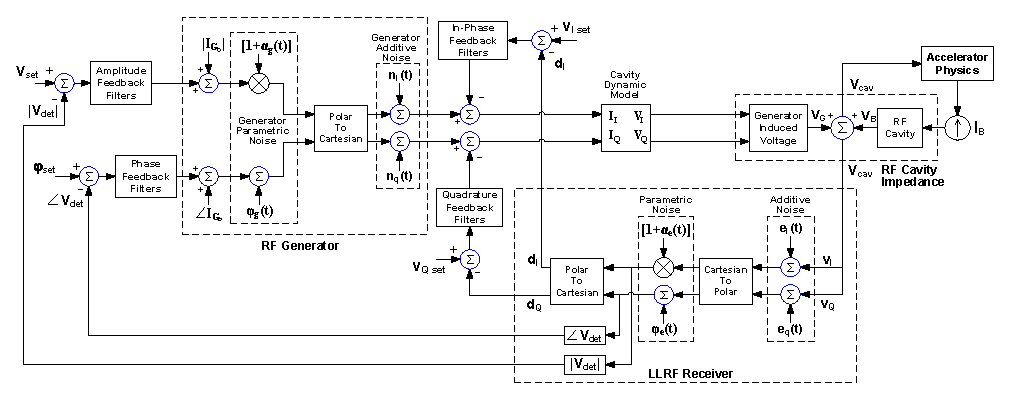
\includegraphics{rfFeedbackModel}
\caption{Rf feedback model used by the {\tt RFMODE} element.}
\label{fig:rfFeedbackModel}
\end{figure}

Normally, the field dumped in the cavity by one particle affects trailing particles in the same turn.
However, if one is also using a \verb|WAKE| or \verb|ZLONGIT| element to simulate the short-range wake of the cavity, this would be double-counting.
In that case, one can use \verb|LONG_RANGE_ONLY=1| to suppress the same-turn effects of the \verb|RFMODE| element.

Two output files are available: the \verb|RECORD| file includes bunch-by-bunch data on the beam-induced fields and the total cavity fields.
The \verb|FEEDBACK_RECORD| file includes tick-by-tick data from the feedback system simulation; {\em writing this file this can significantly impact performance.}

NB: when \verb|BUNCHED_BEAM_MODE| is set to a value other than 1, in order to obtain the effect of several bunches while tracking
only one bunch, the total charge set with the \verb|TOTAL| parameter of the \verb|CHARGE| element should equal the charge in
a single bunch, not the entire beam. However, when \verb|BUNCHED_BEAM_MODE|=1 (allowing an indeterminant number of bunches to be
actually present), then \verb|TOTAL| should be the total for all bunches together.

\vspace*{0.5in}
\vspace*{5mm}

{\bf Explanation of $<$filename$>$=$<$x$>$+$<$y$>$ format:} Several elements in {\tt elegant} make use of data from external files to provide input waveforms.
The external files are SDDS files, which may have many columns.  In order to provide a convenient
way to specify both the filename and the columns to use, we frequently employ $<$filename$>$=$<$x$>$+$<$y$>$ format
for the parameter value.  For example, if the parameter value is \verb|waveform.sdds=t+A|, then it
means that columns \verb|t| and \verb|A| will be taken from file \verb|waveform.sdds|.  The first
column is always the independent variable (e.g., time, position, or frequency), while the second
column is the dependent quantity.




\newpage
\begin{center}{\Large\verb|RFTM110|}\end{center}
\subsection{RFTM110---Tracks through a TM110-mode (deflecting) rf cavity with all magnetic and electric field components.  NOT RECOMMENDED---See below.}
Tracks through a TM110-mode (deflecting) rf cavity with all magnetic and electric field components.  NOT RECOMMENDED---See below.
\\
Parallel capable? : yes\\
GPU capable? : no\\
Back-tracking capable? : no\\
\begin{tabular}{|l|l|l|l|p{\descwidth}|} \hline
Parameter Name & Units & Type & Default & Description \\ \hline 
PHASE & $DEG$ & double &  0.0 & phase  \\ \hline 
TILT & $RAD$ & double &  0.0 & rotation about longitudinal axis  \\ \hline 
FREQUENCY & $HZ$ & double &   2856000000 & frequency  \\ \hline 
VOLTAGE & $V$ & double &  0.0 & peak deflecting voltage  \\ \hline 
PHASE\_REFERENCE &  & long &  \verb|0| & phase reference number (to link with other time-dependent elements)  \\ \hline 
VOLTAGE\_WAVEFORM &  & STRING &   NULL            & $<$filename$>$=$<$x$>$+$<$y$>$ form specification of input file giving voltage waveform factor vs time  \\ \hline 
VOLTAGE\_PERIODIC &  & short &  \verb|0| & If non-zero, voltage waveform is periodic with period given by time span.  \\ \hline 
ALIGN\_WAVEFORMS &  & short &  \verb|0| & If non-zero, waveforms' t=0 is aligned with first bunch arrival time.  \\ \hline 
VOLTAGE\_NOISE &  & double &  0.0 & Rms fractional noise level for voltage.  \\ \hline 
PHASE\_NOISE & $DEG$ & double &  0.0 & Rms noise level for phase.  \\ \hline 
GROUP\_VOLTAGE\_NOISE &  & double &  0.0 & Rms fractional noise level for voltage linked to group.  \\ \hline 
GROUP\_PHASE\_NOISE & $DEG$ & double &  0.0 & Rms noise level for phase linked to group.  \\ \hline 
VOLTAGE\_NOISE\_GROUP &  & long &  \verb|0| & Group number for voltage noise.  \\ \hline 
PHASE\_NOISE\_GROUP &  & long &  \verb|0| & Group number for phase noise.  \\ \hline 
START\_PASS &  & long &   -1              & If non-negative, pass on which to start modeling cavity.  \\ \hline 
END\_PASS &  & long &   -1              & If non-negative, pass on which to end modeling cavity.  \\ \hline 
GROUP &  & string & NULL & Optionally used to assign an element to a group, with a user-defined name.  Group names will appear in the parameter output file in the column ElementGroup  \\ \hline 
\end{tabular}

\vspace*{0.5in}
\documentclass{article}[12pt]

To derive the field expansion, we start with some results from
Jackson\cite{Jackson}, section 8.7.  The longitudinal electric field
for a TM mode is just
\begin{equation}
E_z = - i E_0 \Psi(\rho, \phi) \cos \left(\frac{p \pi z}{d}\right) e^{-i\omega t},
\end{equation}
where $p$ is an integer, $d$ is the length of the cavity, and we use
cylindrical coordinates $(\rho, \phi, z)$.  The factor of $-i$ represents a
choice of sign and phase convention.  We are interested in the
TM110 mode, so we set $p=0$.  In this case, we have
\begin{equation}
E_x = E_y = 0 
\end{equation}
and (using CGS units)
\begin{equation}
\vec{H} = - i E_0 \frac{i \epsilon \omega}{c k^2} \hat{z} \times \nabla \Psi e^{-i \omega t}.
\end{equation}
For a cylindrical cavity, the function $\Psi$ for the $m=1$ aximuthal mode is 
\begin{equation}
\Psi(\rho, \phi) = J_1 (k \rho) \cos \phi,
\end{equation}
where $k = x_{11}/R$, $x_{11}$ is the first zero of $J_1(x)$, and $R$ is the cavity radius.
We don't need to know the cavity radius, since $k = \omega/c$, where $\omega$ is the
resonant frequency.  By choosing $\cos\phi$ for the aximuthal dependence, we'll get 
a magnetic field primarily in the vertical direction.

In MKS units, the magnetic field is
\begin{equation}
\vec{B} = \frac{E_0}{k c} e^{-i \omega t} \left( \hat{\rho} \frac{J_1(k\rho)}{\rho} \sin \phi
        + \hat{\phi} \cos\phi \frac{\partial J_1(k\rho)}{\partial \rho}\right).
\end{equation}

Using {\tt mathematica}, we expanded these expressions to sixth order
in $k*\rho$.  Here, we present only the expressions to second
order. Taking the real parts only, we now have
\begin{eqnarray}
E_z & \approx & \frac{-1}{2} E_0 k \rho \cos \phi \sin \omega t \\
c B_\rho  & \approx & E_0 \left(\frac{1}{2} - \frac{k^2 \rho^2}{16}\right)\sin\phi \cos\omega t \\
c B_\phi  & \approx & E_0 \left(\frac{1}{2} - \frac{3 k^2 \rho^2}{16}\right)\cos\phi \cos\omega t 
\end{eqnarray}
The Cartesian components of $\vec{B}$ can be computed easily
\begin{eqnarray}
c B_x & = & c B_\rho\cos\phi - c B_\phi\sin\phi \\
      & = & \frac{E_0}{8} \rho^2 k^2 \cos\phi \sin\phi \cos\omega t \\
c B_y & = & c B_\rho\sin\phi + c B_\phi\cos\phi \\
      & = & E_0 \left(\frac{1}{2} - \frac{k^2\rho^2 (2 \cos^2\phi + 1)}{16}\right) \cos\omega t 
\end{eqnarray}

The Lorentz force on an electron is $F = -e E_z \hat{z} - e c \vec{\beta} \times \vec{B}$,
giving
\begin{eqnarray}
F_x/e & = & \beta_z c B_y \\
F_y/e & = & -\beta_z c B_x \\
F_z/e & = & -E_z - \beta_x c B_y + \beta_y c B_x 
\end{eqnarray}
We see that for $\rho \rightarrow 0$, we have $E_z = 0$, $B_x = 0$, and
\begin{equation}
c B_y = \frac{E_0}{2} \cos \omega t.
\end{equation}
Hence, for $\omega t=0$ and $E_0>0$ we have $F_x>0$.  This explains
our choice of sign and phase convention above.

\vspace*{0.5in}
\vspace*{5mm}

{\bf Explanation of $<$filename$>$=$<$x$>$+$<$y$>$ format:} Several elements in {\tt elegant} make use of data from external files to provide input waveforms.
The external files are SDDS files, which may have many columns.  In order to provide a convenient
way to specify both the filename and the columns to use, we frequently employ $<$filename$>$=$<$x$>$+$<$y$>$ format
for the parameter value.  For example, if the parameter value is \verb|waveform.sdds=t+A|, then it
means that columns \verb|t| and \verb|A| will be taken from file \verb|waveform.sdds|.  The first
column is always the independent variable (e.g., time, position, or frequency), while the second
column is the dependent quantity.




\newpage
\begin{center}{\Large\verb|RFTMEZ0|}\end{center}
\subsection{RFTMEZ0---A TM-mode RF cavity specified by the on-axis Ez field.}
A TM-mode RF cavity specified by the on-axis Ez field.
\\
Parallel capable? : yes\\
GPU capable? : no\\
Back-tracking capable? : no\\
\begin{tabular}{|l|l|l|l|p{\descwidth}|} \hline
Parameter Name & Units & Type & Default & Description \\ \hline 
L & $M$ & double &  0.0 & length  \\ \hline 
FREQUENCY & $HZ$ & double &   2856000000 & frequency  \\ \hline 
PHASE & $RAD$ & double &  0.0 & phase  \\ \hline 
EZ\_PEAK & $V$ & double &  0.0 & Peak on-axis longitudinal electric field  \\ \hline 
TIME\_OFFSET & $S$ & double &  0.0 & time offset (adds to phase)  \\ \hline 
PHASE\_REFERENCE &  & long &  \verb|0| & phase reference number (to link to other time-dependent elements)  \\ \hline 
DX & $M$ & double &  0.0 & misalignment  \\ \hline 
DY & $M$ & double &  0.0 & misalignment  \\ \hline 
DZ & $M$ & double &  0.0 & misalignment  \\ \hline 
ETILT & $RAD$ & double &  0.0 & misalignment  \\ \hline 
EYAW & $RAD$ & double &  0.0 & misalignment  \\ \hline 
EPITCH & $RAD$ & double &  0.0 & misalignment  \\ \hline 
N\_STEPS &  & long &   100             & number of steps (for nonadaptive integration)  \\ \hline 
RADIAL\_ORDER &  & short &   1               & highest order in off-axis expansion  \\ \hline 
CHANGE\_P0 &  & short &  \verb|0| & does element change central momentum?  \\ \hline 
INPUTFILE &  & STRING &   NULL            & file containing Ez vs z at r=0  \\ \hline 
ZCOLUMN &  & STRING &   NULL            & column containing z values  \\ \hline 
EZCOLUMN &  & STRING &   NULL            & column containing Ez values  \\ \hline 
SOLENOID\_FILE &  & STRING &   NULL            & file containing map of Bz and Br vs z and r.  Each page contains values for a single r.  \\ \hline 
SOLENOID\_ZCOLUMN &  & STRING &   NULL            & column containing z values for solenoid map.  \\ \hline 
SOLENOID\_RCOLUMN &  & STRING &   NULL            & column containing r values for solenoid map.  If omitted, data is assumed to be for r=0 and an on-axis expansion is performed.  \\ \hline 
\end{tabular}

\newpage
\begin{center}{\Large\verb|RFTMEZ0| continued}\end{center}
A TM-mode RF cavity specified by the on-axis Ez field.
\\
\begin{tabular}{|l|l|l|l|p{\descwidth}|} \hline
Parameter Name & Units & Type & Default & Description \\ \hline 
SOLENOID\_BZCOLUMN &  & STRING &   NULL            & column containing Bz values for solenoid map.  \\ \hline 
SOLENOID\_BRCOLUMN &  & STRING &   NULL            & column containing Br values for solenoid map. If omitted, data is assumed to be for r=0 and an on-axis expansion is performed.  \\ \hline 
SOLENOID\_FACTOR &  & double &   1 & factor by which to multiply solenoid fields.  \\ \hline 
SOLENOID\_DX & $M$ & double &  0.0 & misalignment  \\ \hline 
SOLENOID\_DY & $M$ & double &  0.0 & misalignment  \\ \hline 
SOLENOID\_DZ & $M$ & double &  0.0 & misalignment  \\ \hline 
SOLENOID\_ETILT & $RAD$ & double &  0.0 & misalignment  \\ \hline 
SOLENOID\_EYAW & $RAD$ & double &  0.0 & misalignment  \\ \hline 
SOLENOID\_EPITCH & $RAD$ & double &  0.0 & misalignment  \\ \hline 
BX\_STRAY &  & double &  0.0 & Uniform stray horizontal field  \\ \hline 
BY\_STRAY &  & double &  0.0 & Uniform stray vertical field  \\ \hline 
ACCURACY &  & double &   0.0001 & integration accuracy  \\ \hline 
METHOD & $ $ & STRING &   runge-kutta     & integration method (runge-kutta, bulirsch-stoer, non-adaptive runge-kutta, modified midpoint)  \\ \hline 
FIDUCIAL &  & STRING &   t,median        & \{t$|$p\},\{median$|$min$|$max$|$ave$|$first$|$light\} (e.g., "t,median")  \\ \hline 
FIELD\_TEST\_FILE &  & STRING &   NULL            & filename for output of test fields (r=0)  \\ \hline 
GROUP &  & string & NULL & Optionally used to assign an element to a group, with a user-defined name.  Group names will appear in the parameter output file in the column ElementGroup  \\ \hline 
\end{tabular}

\newpage
\begin{center}{\Large\verb|RIMULT|}\end{center}
\subsection{RIMULT---Multiplies radiation integrals by a given factor.  Use to compute emittance for collection of various types of cells.}
Multiplies radiation integrals by a given factor.  Use to compute emittance for collection of various types of cells.
\\
Parallel capable? : yes\\
GPU capable? : no\\
Back-tracking capable? : no\\
\begin{tabular}{|l|l|l|l|p{\descwidth}|} \hline
Parameter Name & Units & Type & Default & Description \\ \hline 
FACTOR &  & double &   1 & factor  \\ \hline 
GROUP &  & string & NULL & Optionally used to assign an element to a group, with a user-defined name.  Group names will appear in the parameter output file in the column ElementGroup  \\ \hline 
\end{tabular}

\newpage
\begin{center}{\Large\verb|RMDF|}\end{center}
\subsection{RMDF---A linearly-ramped electric field deflector, using an approximate analytical solution FOR LOW ENERGY PARTICLES.}
A linearly-ramped electric field deflector, using an approximate analytical solution FOR LOW ENERGY PARTICLES.
\\
Parallel capable? : no\\
GPU capable? : no\\
Back-tracking capable? : no\\
\begin{tabular}{|l|l|l|l|p{\descwidth}|} \hline
Parameter Name & Units & Type & Default & Description \\ \hline 
L & $M$ & double &  0.0 & length  \\ \hline 
TILT & $RAD$ & double &  0.0 & rotation about longitudinal axis  \\ \hline 
RAMP\_TIME & $S$ & double &   1e-09 & length of ramp  \\ \hline 
VOLTAGE & $V$ & double &  0.0 & full voltage  \\ \hline 
GAP & $M$ & double &   0.01 & gap between plates  \\ \hline 
TIME\_OFFSET & $S$ & double &  0.0 & time offset of ramp start  \\ \hline 
N\_SECTIONS &  & long &   10              & number of sections  \\ \hline 
PHASE\_REFERENCE &  & long &  \verb|0| & phase reference number (to link with other time-dependent elements)  \\ \hline 
DX & $M$ & double &  0.0 & misalignment  \\ \hline 
DY & $M$ & double &  0.0 & misalignment  \\ \hline 
GROUP &  & string & NULL & Optionally used to assign an element to a group, with a user-defined name.  Group names will appear in the parameter output file in the column ElementGroup  \\ \hline 
\end{tabular}

\newpage
\begin{center}{\Large\verb|ROTATE|}\end{center}
\subsection{ROTATE---An element that rotates the beam about the longitudinal axis.}
An element that rotates the beam about the longitudinal axis.
\\
Parallel capable? : yes\\
GPU capable? : yes\\
Back-tracking capable? : yes\\
\begin{tabular}{|l|l|l|l|p{\descwidth}|} \hline
Parameter Name & Units & Type & Default & Description \\ \hline 
TILT & $RAD$ & double &  0.0 & rotation about longitudinal axis  \\ \hline 
EXCLUDE\_FLOOR &  & short &  \verb|0| & if non-zero, does not affect the floor coordinates  \\ \hline 
EXCLUDE\_OPTICS &  & short &  \verb|0| & if non-zero, does not affect the optics (i.e., transfer matrix is unit matrix)  \\ \hline 
GROUP &  & string & NULL & Optionally used to assign an element to a group, with a user-defined name.  Group names will appear in the parameter output file in the column ElementGroup  \\ \hline 
\end{tabular}

\vspace*{0.5in}
The sign convention for the {\tt TILT}  parameter is confusing on this element.
In particular, a positive {\tt TILT} rotates the beam counter-clockwise about the
longitudinal axis.  This is the opposite sense to rotations of elements, where a 
positive {\tt TILT} rotates the element clockwise about the longitudinal axis.

Hence, if one wanted to rotate a series of elements by 0.1 rad, one could do the
following:
\begin{verbatim}
ROT1: ROTATE,TILT=0.1
ROT2: ROTATE,TILT=-0.1
BL: line=(ROT1,...,ROT2)
\end{verbatim}
The {\tt TILT} value for {\tt ROT1} is the same (including the sign) as the individual
{\tt TILT} values one would give to all the elements represented by \verb|...|.


\newpage
\begin{center}{\Large\verb|SAMPLE|}\end{center}
\subsection{SAMPLE---An element that reduces the number of particles in the beam by interval-based or random sampling.}
An element that reduces the number of particles in the beam by interval-based or random sampling.
\\
Parallel capable? : yes\\
GPU capable? : no\\
Back-tracking capable? : no\\
\begin{tabular}{|l|l|l|l|p{\descwidth}|} \hline
Parameter Name & Units & Type & Default & Description \\ \hline 
FRACTION &  & double &   1 & fraction to keep  \\ \hline 
INTERVAL &  & long &   1               & interval between sampled particles  \\ \hline 
GROUP &  & string & NULL & Optionally used to assign an element to a group, with a user-defined name.  Group names will appear in the parameter output file in the column ElementGroup  \\ \hline 
\end{tabular}

\newpage
\begin{center}{\Large\verb|SBEN|}\end{center}
\subsection{SBEN---A sector dipole implemented as a matrix, up to 2nd order. Use CSBEND for symplectic tracking.}
A sector dipole implemented as a matrix, up to 2nd order. Use CSBEND for symplectic tracking.
\\
Parallel capable? : yes\\
GPU capable? : yes\\
Back-tracking capable? : yes\\
\begin{tabular}{|l|l|l|l|p{\descwidth}|} \hline
Parameter Name & Units & Type & Default & Description \\ \hline 
L & $M$ & double &  0.0 & arc length  \\ \hline 
ANGLE & $RAD$ & double &  0.0 & bend angle  \\ \hline 
K1 & $1/M^{2}$ & double &  0.0 & geometric focusing strength  \\ \hline 
E1 & $RAD$ & double &  0.0 & entrance edge angle  \\ \hline 
E2 & $RAD$ & double &  0.0 & exit edge angle  \\ \hline 
TILT & $RAD$ & double &  0.0 & rotation about incoming longitudinal axis  \\ \hline 
K2 & $1/M^{3}$ & double &  0.0 & geometric sextupole strength  \\ \hline 
H1 & $1/M$ & double &  0.0 & entrance pole-face curvature  \\ \hline 
H2 & $1/M$ & double &  0.0 & exit pole-face curvature  \\ \hline 
HGAP & $M$ & double &  0.0 & half-gap between poles  \\ \hline 
FINT &  & double &   0.5 & edge-field integral  \\ \hline 
DX & $M$ & double &  0.0 & misaligment of entrance  \\ \hline 
DY & $M$ & double &  0.0 & misalignment of entrance  \\ \hline 
DZ & $M$ & double &  0.0 & misalignment of entrance  \\ \hline 
FSE &  & double &  0.0 & fractional strength error of all components  \\ \hline 
FSE\_DIPOLE &  & double &  0.0 & fractional strength error of dipole component  \\ \hline 
FSE\_QUADRUPOLE &  & double &  0.0 & fractional strength error of quadrupole component  \\ \hline 
ETILT & $RAD$ & double &  0.0 & error rotation about incoming longitudinal axis  \\ \hline 
ETILT\_SIGN &  & short &   -1              & Sign of ETILT relative to TILT. -1 is the old convention and is the default for backwards compatibility  \\ \hline 
EDGE1\_EFFECTS &  & short &   1               & include entrance edge effects?  \\ \hline 
EDGE2\_EFFECTS &  & short &   1               & include exit edge effects?  \\ \hline 
ORDER &  & short &  \verb|0| & matrix order  \\ \hline 
EDGE\_ORDER &  & short &  \verb|0| & edge matrix order  \\ \hline 
TRANSPORT &  & short &  \verb|0| & use (incorrect) TRANSPORT equations for T436 of edge?  \\ \hline 
\end{tabular}

\newpage
\begin{center}{\Large\verb|SBEN| continued}\end{center}
A sector dipole implemented as a matrix, up to 2nd order. Use CSBEND for symplectic tracking.
\\
\begin{tabular}{|l|l|l|l|p{\descwidth}|} \hline
Parameter Name & Units & Type & Default & Description \\ \hline 
USE\_BN &  & short &  \verb|0| & use B1 and B2 instead of K1 and K2 values?  \\ \hline 
B1 & $1/M$ & double &  0.0 & K1 = B1/rho, where rho is bend radius  \\ \hline 
B2 & $1/M^{2}$ & double &  0.0 & K2 = B2/rho  \\ \hline 
GROUP &  & string & NULL & Optionally used to assign an element to a group, with a user-defined name.  Group names will appear in the parameter output file in the column ElementGroup  \\ \hline 
\end{tabular}

\vspace*{0.5in}
{\em Special note about splitting dipoles}: when dipoles are long, it is
common to want to split them into several pieces, to get a better look
at the interior optics.  When doing this, care must be exercised not
to change the optics.  {\tt elegant} has some special features that
are designed to reduce or manage potential problems. At issue is the
need to turn off edge effects between the portions of the same dipole.

First, one can simply use the \verb|divide_elements| command to set up
the splitting.  Using this command, {\tt elegant} takes care of everything.

Second, one can use a series of dipoles {\em with the same name}.  In this case,
elegant automatically turns off interior edge effects.  This is true when the
dipole elements directly follow one another or are separated by a MARK element.

Third, one can use a series of dipoles with different names.  In this case, you
must also use the \verb|EDGE1_EFFECTS| and \verb|EDGE2_EFFECTS| parameters to
turn off interior edge effects.  

\newpage
\begin{center}{\Large\verb|SCATTER|}\end{center}
\subsection{SCATTER---A scattering element to add gaussian random numbers to particle coordinates.}
A scattering element to add gaussian random numbers to particle coordinates.
\\
Parallel capable? : yes\\
GPU capable? : no\\
Back-tracking capable? : no\\
\begin{tabular}{|l|l|l|l|p{\descwidth}|} \hline
Parameter Name & Units & Type & Default & Description \\ \hline 
X & $M$ & double &  0.0 & rms scattering level for x  \\ \hline 
XP &  & double &  0.0 & rms scattering level for x'  \\ \hline 
Y & $M$ & double &  0.0 & rms scattering level for y  \\ \hline 
YP &  & double &  0.0 & rms scattering level for y'  \\ \hline 
DP &  & double &  0.0 & rms scattering level for (p-pCentral)/pCentral  \\ \hline 
PROBABILITY &  & double &   1 & Probability that any particle will be selected for scattering.  \\ \hline 
STARTONPASS &  & long &  \verb|0| & Pass number to start on.  \\ \hline 
ENDONPASS &  & long &   -1              & Pass number to end on (inclusive).  Ignored if negative.  \\ \hline 
GROUP &  & string & NULL & Optionally used to assign an element to a group, with a user-defined name.  Group names will appear in the parameter output file in the column ElementGroup  \\ \hline 
\end{tabular}

\newpage
\begin{center}{\Large\verb|SCMULT|}\end{center}
\subsection{SCMULT---Tracks through a zero length multipole to simulate space charge effects}
Tracks through a zero length multipole to simulate space charge effects
\\
Parallel capable? : yes\\
GPU capable? : no\\
Back-tracking capable? : no\\
\begin{tabular}{|l|l|l|l|p{\descwidth}|} \hline
Parameter Name & Units & Type & Default & Description \\ \hline 
GROUP &  & string & NULL & Optionally used to assign an element to a group, with a user-defined name.  Group names will appear in the parameter output file in the column ElementGroup  \\ \hline 
\end{tabular}

\vspace*{0.5in}


This element simulates transverse space charge (SC) kick using
K.Y. Ng's formula ( K.Y. Ng, FNAL, private communication). 
{\bf N.B.: This element is not designed for space charge
calculations in guns or linacs.  It is only intended for
simulating space charge in rings. }

The linear SC force is given by:
\[
\Delta x'=\frac{K_{sc}Le^{-z^2/(2\sigma_z^2)}}{\sqrt{2\pi}\sigma_z}
\frac{x}{\sigma_x(\sigma_x+\sigma_y)}
\]
\begin{equation}
\Delta y'=\frac{K_{sc}Le^{-z^2/(2\sigma_z^2)}}{\sqrt{2\pi}\sigma_z}
\frac{y}{\sigma_y(\sigma_x+\sigma_y)}
\end{equation}
where $K_{sc}=\frac{2Nr_e}{\gamma^3\beta^2}$,
$L$ is the integrating length, $\sigma_{x,y,z}$ are rms beam size.

The non-linear SC force is given by:
\[
\Delta x'=\frac{K_{sc}Le^{-z^2/(2\sigma_z^2)}}{2\sigma_z\sqrt{\sigma_x^2-\sigma_y^2}}
Im\left [ w\left( \frac{x+iy}{\sqrt{2(\sigma_x^2-\sigma_y^2)}} \right)
-e^{-\frac{x^2}{2 \sigma_x^2}-\frac{y^2}{2 \sigma_y^2}}
w\left(\frac{x\frac{\sigma_y}{\sigma_x}+iy\frac{\sigma_x}{\sigma_y}}
{\sqrt{2(\sigma_x^2-\sigma_y^2)}}\right)\right ]
\]
\begin{equation}
\Delta y'=\frac{K_{sc}Le^{-z^2/(2\sigma_z^2)}}{2\sigma_z\sqrt{\sigma_x^2-\sigma_y^2}}
Re\left [ w\left( \frac{x+iy}{\sqrt{2(\sigma_x^2-\sigma_y^2)}} \right)
-e^{-\frac{x^2}{2 \sigma_x^2}-\frac{y^2}{2 \sigma_y^2}}
w\left(\frac{x\frac{\sigma_y}{\sigma_x}+iy\frac{\sigma_x}{\sigma_y}}
{\sqrt{2(\sigma_x^2-\sigma_y^2)}}\right)\right ]
\label{equa2}
\end{equation}
where $w(z)$ is the complex error function
\begin{equation}
w(z)=e^{-z^2}\left [ 1+\frac{2i}{\sqrt{\pi}}\int\limits_0^z e^{\zeta^2}d\zeta\right ]
\end{equation}
Equation~\ref{equa2} appear to diverge when $\sigma_x=\sigma_y$. In fact, this is not
true, because the expressions inside the square brackets will provide zero too at
$\sigma_x=\sigma_y$ to cancel the poles outside. In our code, we calculate this equation
at  $1.01 \sigma_x$ and $0.99\sigma_x$, and average the total effects. 
 
To invoke the calculation, one must use set up command
``insert\_sceffects'' proceed ``run\_setup'' and ``Twiss\_output''
command proceed ``track''.


\newpage
\begin{center}{\Large\verb|SCRAPER|}\end{center}
\subsection{SCRAPER---A collimating element that sticks into the beam from one side only.  The directions 0, 1, 2, and 3 are from +x, +y, -x, and -y, respectively.}
A collimating element that sticks into the beam from one side only.  The directions 0, 1, 2, and 3 are from +x, +y, -x, and -y, respectively.
\\
Parallel capable? : yes\\
GPU capable? : yes\\
Back-tracking capable? : yes\\
\begin{tabular}{|l|l|l|l|p{\descwidth}|} \hline
Parameter Name & Units & Type & Default & Description \\ \hline 
L & $M$ & double &  0.0 & length  \\ \hline 
XO & $M$ & double &  0.0 & radiation length  \\ \hline 
ENERGY\_DECAY &  & long &  \verb|0| & If nonzero, then particles will lose energy due to material using a simple exponential model.  \\ \hline 
ENERGY\_STRAGGLE &  & long &  \verb|0| & Use simple-minded energy straggling model coupled with ENERGY\_DECAY=1?  \\ \hline 
NUCLEAR\_BREMSSTRAHLUNG &  & long &  \verb|0| & Model energy loss to nuclear bremsstrahlung? If enabled, set ENERGY\_DECAY=0 to disable simpler model.  \\ \hline 
ELECTRON\_RECOIL &  & long &  \verb|0| & If non-zero, electron recoil during Coulomb scattering is included (results in energy change).  \\ \hline 
Z &  & long &  \verb|0| & Atomic number  \\ \hline 
A & $AMU$ & double &  0.0 & Atomic mass  \\ \hline 
RHO & $KG/M^3$ & double &  0.0 & Density  \\ \hline 
PLIMIT &  & double &   0.05 & Probability cutoff for each slice  \\ \hline 
POSITION & $M$ & double &  0.0 & position of edge  \\ \hline 
DX & $M$ & double &  0.0 & misalignment  \\ \hline 
DY & $M$ & double &  0.0 & misalignment  \\ \hline 
INSERT\_FROM &  & STRING &   NULL            & direction from which inserted (+x, -x, x, +y, -y, y)  \\ \hline 
DIRECTION &  & long &   -1              & Deprecated. use INSERT\_FROM.  \\ \hline 
GROUP &  & string & NULL & Optionally used to assign an element to a group, with a user-defined name.  Group names will appear in the parameter output file in the column ElementGroup  \\ \hline 
\end{tabular}

\vspace*{0.5in}
The method used for material modeling is the same as that used for the \verb|MATTER| element.

The \verb|DIRECTION| parameter is deprecated and the more versatile \verb|INSERT_FROM| parameter
should be used instead.
The values for the latter determine from which side the scraper is inserted.
E.g., \verb|INSERT_FROM="-x",POSITION=0.005| means the scraper is inserted from the negative x side
and extends from $x=-\infty$ to $x=-0.005$m.

\verb|INSERT_FROM="x"| or \verb|INSERT_FROM="y"| means the scraper is inserted from both sides, in which case the interpretation
of the position is different. 
E.g., \verb|INSERT_FROM="x",POSITION=0.005| means that only the region $x:[-0.005, 0.005]$m is clear.

\newpage
\begin{center}{\Large\verb|SCRIPT|}\end{center}
\subsection{SCRIPT---An element that allows transforming the beam using an external script.}
An element that allows transforming the beam using an external script.
\\
Parallel capable? : yes\\
GPU capable? : no\\
Back-tracking capable? : yes\\
\begin{tabular}{|l|l|l|l|p{\descwidth}|} \hline
Parameter Name & Units & Type & Default & Description \\ \hline 
L & $M$ & double &  0.0 & Length to be used for matrix-based operations such as twiss parameter computation.  \\ \hline 
COMMAND &  & STRING &   NULL            & SDDS-compliant command to apply to the beam.  Use the sequence \%i to represent the input filename and \%o to represent the output filename.  \\ \hline 
USE\_CSH &  & short &   1               & Use C-shell for execution (may be slower)?  \\ \hline 
VERBOSITY &  & short &  \verb|0| & Set the verbosity level.  \\ \hline 
RPN\_PARAMETERS &  & short &  \verb|0| & If nonzero, then parameters from the script output file are loaded into RPN variables.  \\ \hline 
START\_PASS &  & long &   -1              & Start script action on this pass.  Before that, behaves like a drift space.  \\ \hline 
END\_PASS &  & long &   -1              & End script action after this pass.  Before that, behaves like a drift space.  \\ \hline 
PASS\_INTERVAL &  & long &   -1              & Execute script only every Nth pass following START\_PASS, including START\_PASS. Otherwise, behaves like a drift space.  \\ \hline 
ON\_PASS &  & long &   -1              & Perform script action only on this pass, overriding other pass controls. Other than that, behaves like a drift space.  \\ \hline 
DIRECTORY &  & STRING &   NULL            & Directory in which to place input and output files.  If blank, the present working directory is used.  \\ \hline 
ROOTNAME &  & STRING &   NULL            & Rootname for use in naming input and output files.  \%s may be used to represent the run rootname.  \\ \hline 
\end{tabular}

\newpage
\begin{center}{\Large\verb|SCRIPT| continued}\end{center}
An element that allows transforming the beam using an external script.
\\
\begin{tabular}{|l|l|l|l|p{\descwidth}|} \hline
Parameter Name & Units & Type & Default & Description \\ \hline 
INPUT\_EXTENSION &  & STRING &   in              & Extension for the script input file.  \\ \hline 
OUTPUT\_EXTENSION &  & STRING &   out             & Extension for the script output file.  \\ \hline 
KEEP\_FILES &  & short &  \verb|0| & If nonzero, then script input and output files are not deleted after use.  By default, they are deleted.  \\ \hline 
DRIFT\_MATRIX &  & short &  \verb|0| & If nonzero, then for non-tracking calculations the element is treated as a drift space.  \\ \hline 
USE\_PARTICLE\_ID &  & short &   1               & If nonzero, then the output file will supply particle IDs. Otherwise, particles are renumbered.  \\ \hline 
NO\_NEW\_PARTICLES &  & short &   1               & If nonzero, then no new particles will be added in the script output file.  \\ \hline 
DETERMINE\_LOSSES\_FROM\_PID &  & short &   1               & If nonzero and if USE\_PARTICLE\_ID is nonzero, then particleID data from script output is used to determine which particles were lost.  \\ \hline 
SOFT\_FAILURE &  & short &   1               & If output file does not exist or can't be read, consider all particles lost.  \\ \hline 
NP0 &  & double &  0.0 & User-defined numerical parameter for command substitution for sequence \%np0  \\ \hline 
NP1 &  & double &  0.0 & User-defined numerical parameter for command substitution for sequence \%np1  \\ \hline 
NP2 &  & double &  0.0 & User-defined numerical parameter for command substitution for sequence \%np2  \\ \hline 
\end{tabular}

\newpage
\begin{center}{\Large\verb|SCRIPT| continued}\end{center}
An element that allows transforming the beam using an external script.
\\
\begin{tabular}{|l|l|l|l|p{\descwidth}|} \hline
Parameter Name & Units & Type & Default & Description \\ \hline 
NP3 &  & double &  0.0 & User-defined numerical parameter for command substitution for sequence \%np3  \\ \hline 
NP4 &  & double &  0.0 & User-defined numerical parameter for command substitution for sequence \%np4  \\ \hline 
NP5 &  & double &  0.0 & User-defined numerical parameter for command substitution for sequence \%np5  \\ \hline 
NP6 &  & double &  0.0 & User-defined numerical parameter for command substitution for sequence \%np6  \\ \hline 
NP7 &  & double &  0.0 & User-defined numerical parameter for command substitution for sequence \%np7  \\ \hline 
NP8 &  & double &  0.0 & User-defined numerical parameter for command substitution for sequence \%np8  \\ \hline 
NP9 &  & double &  0.0 & User-defined numerical parameter for command substitution for sequence \%np9  \\ \hline 
SP0 &  & STRING &   NULL            & User-defined string parameter for command substitution for sequence \%sp0  \\ \hline 
SP1 &  & STRING &   NULL            & User-defined string parameter for command substitution for sequence \%sp1  \\ \hline 
SP2 &  & STRING &   NULL            & User-defined string parameter for command substitution for sequence \%sp2  \\ \hline 
SP3 &  & STRING &   NULL            & User-defined string parameter for command substitution for sequence \%sp3  \\ \hline 
SP4 &  & STRING &   NULL            & User-defined string parameter for command substitution for sequence \%sp4  \\ \hline 
\end{tabular}

\newpage
\begin{center}{\Large\verb|SCRIPT| continued}\end{center}
An element that allows transforming the beam using an external script.
\\
\begin{tabular}{|l|l|l|l|p{\descwidth}|} \hline
Parameter Name & Units & Type & Default & Description \\ \hline 
SP5 &  & STRING &   NULL            & User-defined string parameter for command substitution for sequence \%sp5  \\ \hline 
SP6 &  & STRING &   NULL            & User-defined string parameter for command substitution for sequence \%sp6  \\ \hline 
SP7 &  & STRING &   NULL            & User-defined string parameter for command substitution for sequence \%sp7  \\ \hline 
SP8 &  & STRING &   NULL            & User-defined string parameter for command substitution for sequence \%sp8  \\ \hline 
SP9 &  & STRING &   NULL            & User-defined string parameter for command substitution for sequence \%sp9  \\ \hline 
GROUP &  & string & NULL & Optionally used to assign an element to a group, with a user-defined name.  Group names will appear in the parameter output file in the column ElementGroup  \\ \hline 
\end{tabular}

\vspace*{0.5in}
This element allows expanding {\tt elegant} by using external scripts
(or programs) as elements in a beamline.    Here are requirements for the 
script:
\begin{itemize}
\item It must be executable from the commandline.
\item It must read the initial particle distribution from an SDDS file.
This file will have the usual columns that an {\tt elegant} phase-space
output file  has, along with the parameter {\tt Charge} giving the 
beam charge in Coulombs. The file will contain a single data page.
\item It must write the final particle distribution to an SDDS file.
This file should have all of the columns and parameters that appear in the
initial distribution file.  Additional columns and parameters will be ignored,
as will all pages but the first. 
\item The {\tt Charge} parameter in the file is used to determine the total beam charge; the script must ensure that
  this parameter is set correctly; when particles are lost or created, simply copying or retaining the value from the
  input file will not be correct. Normally, the charge per particle is constant in simulations. Hence, if {\tt elegant}
  sees a change in charge per particle after the {\tt SCRIPT} element, it issues a warning.
\end{itemize}

The {\tt SCRIPT} element works best if the script accepts commandline
arguments.  In this case, the {\tt COMMAND} parameter is used to
provide a template for creating a command to run the script.  The {\tt COMMAND}
string may contain the following substitutable fields:
\begin{enumerate}
\item \verb|%i| --- Will be replaced by the name of the input file to the script.
({\tt elegant} writes the initial particle distribution to this file.)
\item \verb|%o| --- Will be replaced by the name of the output file from the script.
({\tt elegant} expects the script to write the final particle distribution to this file.)
\item \verb|%p| --- Will be replaced by the pass number, which starts from 0.
\item \verb|%c| --- Will be replaced by the occurrence number of the element, which starts from 1.
\item \verb|%b| --- Will be replaced by 0 (1) for forward (backward) tracking.
\item \verb|%np0|, \verb|%np1|, ..., \verb|%np9| --- Will be replaced by the value of
 Numerical Parameter 0, 1, ..., 9.  This can be used to pass to the script values that
 are parameters of the element definition.  For example, if one wanted to vary parameters 
 or add errors to the parameter, one would use this facility.
\item \verb|%sp0|,  \verb|%sp1|, ..., \verb|%sp9| --- Will be replaced by the value of
 String Parameter 0, 1, ..., 9.  This can be used to pass to the script values that
 are parameters of the element definition. 
\end{enumerate}

In some cases, one may wish to keep the input file delivered to the \verb|SCRIPT| as
well as the output file returned by it. This is facilitated by using the \verb|ROOTNAME| 
parameter, which allows specifying the rootname for these files, as well as the
\verb|INPUT_EXTENSION| and \verb|OUTPUT_EXTENSION| parameters.
The \verb|ROOTNAME| parameter may contain a simple string, but may also contain several
substitutible  fields:
\begin{itemize}
\item \verb|%s| --- The global rootname, which may be given by the \verb|rootname| parameter
  in the \verb|run_setup| command.
\item \verb|%p| --- The pass index.
\item \verb|%ld| --- The occurence number of the element.
\end{itemize}

Here's an example of a {\tt SCRIPT} {\tt COMMAND}:
\begin{flushleft}
\begin{verbatim}
myScript -input %i -output %o -accuracy %np0 -type %sp0
\end{verbatim}
\end{flushleft}
In this example, the script {\tt myScript} takes four commandline arguments, giving
the names of the input and output files, an accuracy requirement, and a type specifier.
By default, {\tt elegant} will choose unique, temporary filenames to use in communicating
with the script.  The actual command when executed might be something like
\begin{flushleft}
\begin{verbatim}
myScript -input tmp391929.1 -output tmp391929.2 -accuracy 1.5e-6 -type scraper
\end{verbatim}
\end{flushleft}
where for this example I've assumed {\tt NP0=1.5e-6} and {\tt SP0=''scraper''}.

If you have a program (e.g., a FORTRAN program) that does not accept
commandline arguments, you can easily wrap it in a Tcl/Tk simple script to
handle this.  Alternatively, you can force {\tt elegant} to use specified 
files for communicating with such a script.  This is done using the {\tt ROOTNAME},
{\tt INPUT\_EXTENSION}, and {\tt OUTPUT\_EXTENSION} parameters.
So if your program was {\tt crass} and it expected its input (output) in files
{\tt crass.in} ({\tt crass.out}), then you'd use
\begin{flushleft}
\begin{verbatim}
S1: script,command=''crass'',rootname=''crass'',input_extension=''in'',&
output_extension=''out''
\end{verbatim}
\end{flushleft}

For purposes of computing concatenated transport matrices, Twiss
parameters, response matrices, etc., {\tt elegant} will perform
initial tracking through the \verb|SCRIPT| element using an ensemble
of 25 particles.  If this is not desirable, then set the parameter
\verb|DRIFT_MATRIX| to a non-zero value.  This will force
\verb|elegant| to treat the element as a drift space for any
calculations that involve transport matrices.  Examples of where one
might want to use this feature would be a \verb|SCRIPT| that involves
randomization (e.g., scattering), particle loss, or particle creation.

If non-zero, the \verb|RPN_PARAMETERS| parameter directs \verb|elegant| to load all numerical
SDDS parameter values from the script output file into \verb|rpn| variables, where they may be used for
optimization. This provides the user the ability to perform script-based analysis of particle distributions and
then optimize the results of that analysis.
(Typically in this case the script does not actually transform the particle coordinates, but simply copies them
from the input file to the output file.)
The names of the variables are of the form {\em ElementName}\#{\em N}.{\em ParameterName}, where
{\em N} is the occurrence number of the script element (usually 1 if there is only one instance).


\newpage
\begin{center}{\Large\verb|SEXT|}\end{center}
\subsection{SEXT---A sextupole implemented as a matrix, up to 3rd order. Use KSEXT for symplectic tracking.}
A sextupole implemented as a matrix, up to 3rd order. Use KSEXT for symplectic tracking.
\\
Parallel capable? : yes\\
GPU capable? : yes\\
Back-tracking capable? : yes\\
\begin{tabular}{|l|l|l|l|p{\descwidth}|} \hline
Parameter Name & Units & Type & Default & Description \\ \hline 
L & $M$ & double &  0.0 & length  \\ \hline 
K2 & $1/M^{3}$ & double &  0.0 & geometric strength  \\ \hline 
K1 & $1/M^{2}$ & double &  0.0 & geometric quadrupole strength error. See notes below!  \\ \hline 
J1 & $1/M^{2}$ & double &  0.0 & geometric skew quadrupole strength error. See notes below!  \\ \hline 
TILT & $RAD$ & double &  0.0 & rotation about longitudinal axis  \\ \hline 
DX & $M$ & double &  0.0 & misalignment  \\ \hline 
DY & $M$ & double &  0.0 & misalignment  \\ \hline 
DZ & $M$ & double &  0.0 & misalignment  \\ \hline 
FSE &  & double &  0.0 & fractional strength error  \\ \hline 
FFRINGE &  & double &  0.0 & Length occupied by linear fringe regions as fraction hard-edge length L.  \\ \hline 
ORDER &  & short &  \verb|0| & matrix order  \\ \hline 
GROUP &  & string & NULL & Optionally used to assign an element to a group, with a user-defined name.  Group names will appear in the parameter output file in the column ElementGroup  \\ \hline 
\end{tabular}

\vspace*{0.5in}
This element simulates a sextupole using a matrix, up to third order.

The \verb|K1| and \verb|J1| parameters allow introducing normal and skew quadrupole {\bf error} terms.
The matrix expressions assume that
these are weak effects and high accuracy should not be expected if this is not true.
If \verb|K1| is significant, then use of the \verb|KQUSE| element is preferred.


\newpage
\begin{center}{\Large\verb|SHRFDF|}\end{center}
\subsection{SHRFDF---Simulation through space harmonics of zero length deflecting cavity.}
Simulation through space harmonics of zero length deflecting cavity.
\\
Parallel capable? : yes\\
GPU capable? : no\\
Back-tracking capable? : no\\
\begin{tabular}{|l|l|l|l|p{\descwidth}|} \hline
Parameter Name & Units & Type & Default & Description \\ \hline 
FACTOR &  & double &   1 & A factor by which to multiply all components.  \\ \hline 
TILT & $RAD$ & double &  0.0 & rotation about longitudinal axis  \\ \hline 
PERIOD\_LENGTH & $M$ & double &  0.0 & cavity period length, or cell length  \\ \hline 
PERIOD\_PHASE & $RAD$ & double &  0.0 & cavity period phase advance, or so-called working mode  \\ \hline 
V0 & $V$ & double &  0.0 & effective voltage of space harmonic n=0  \\ \hline 
V1 & $V$ & double &  0.0 & effective voltage of space harmonic n=1  \\ \hline 
V2 & $V$ & double &  0.0 & effective voltage of space harmonic n=2  \\ \hline 
V3 & $V$ & double &  0.0 & effective voltage of space harmonic n=3  \\ \hline 
V4 & $V$ & double &  0.0 & effective voltage of space harmonic n=4  \\ \hline 
V5 & $V$ & double &  0.0 & effective voltage of space harmonic n=5  \\ \hline 
V6 & $V$ & double &  0.0 & effective voltage of space harmonic n=6  \\ \hline 
V7 & $V$ & double &  0.0 & effective voltage of space harmonic n=7  \\ \hline 
V8 & $V$ & double &  0.0 & effective voltage of space harmonic n=8  \\ \hline 
V9 & $V$ & double &  0.0 & effective voltage of space harmonic n=9  \\ \hline 
PHASE0 & $HZ$ & double &  0.0 & Phase of space harmonic n=0  \\ \hline 
PHASE1 & $HZ$ & double &  0.0 & Phase of space harmonic n=1  \\ \hline 
PHASE2 & $HZ$ & double &  0.0 & Phase of space harmonic n=2  \\ \hline 
PHASE3 & $HZ$ & double &  0.0 & Phase of space harmonic n=3  \\ \hline 
PHASE4 & $HZ$ & double &  0.0 & Phase of space harmonic n=4  \\ \hline 
PHASE5 & $HZ$ & double &  0.0 & Phase of space harmonic n=5  \\ \hline 
PHASE6 & $HZ$ & double &  0.0 & Phase of space harmonic n=6  \\ \hline 
PHASE7 & $HZ$ & double &  0.0 & Phase of space harmonic n=7  \\ \hline 
\end{tabular}

\newpage
\begin{center}{\Large\verb|SHRFDF| continued}\end{center}
Simulation through space harmonics of zero length deflecting cavity.
\\
\begin{tabular}{|l|l|l|l|p{\descwidth}|} \hline
Parameter Name & Units & Type & Default & Description \\ \hline 
PHASE8 & $HZ$ & double &  0.0 & Phase of space harmonic n=8  \\ \hline 
PHASE9 & $HZ$ & double &  0.0 & Phase of space harmonic n=9  \\ \hline 
PHASE\_REFERENCE &  & long &  \verb|0| & phase reference number (to link with other time-dependent elements)  \\ \hline 
GROUP &  & string & NULL & Optionally used to assign an element to a group, with a user-defined name.  Group names will appear in the parameter output file in the column ElementGroup  \\ \hline 
\end{tabular}

\vspace*{0.5in}
This element simulates an rf deflector with specified space harmonic parameters (voltage, phase).

The thin kicks from the fundamental deflecting mode are the same as for the element RFDF. The thin kicks from the space harmonics ($n\ge 1$) are \cite{Sun-NAPAC19}

\begin{equation}
\begin{split}
& \Delta P_x  = -\frac{\partial ({\bf H} - H_0)}{\partial x} \\
 &= \sum_{n=1}^{\infty} -q \bar{ V_n} \cdot \sin (k_n z + \phi_n) \cdot (\frac{1}{2}\alpha_n + \frac{1}{16}\alpha_n^3 \cdot (3x^2 + y^2))
\end{split}
\end{equation}


\begin{equation}
\begin{split}
& \Delta P_z = -\frac{\partial ({\bf H} - H_0)}{\partial z} = \sum_{n=1}^{\infty} -q \bar{ V_n} \cdot k_n \cdot \cos (k_n z + \phi_n) \\
&\cdot (\frac{1}{2}\alpha_n \cdot x + \frac{1}{16}\alpha_n^3 \cdot (x^2 + y^2)\cdot x)
\end{split}
\end{equation} 

The wave numbers $k_n$ and $\alpha_n$ are listed below.

\begin{equation}\label{Equa1}
k_n = \frac{\varphi_0 + 2\pi n}{d}
\end{equation} 

\begin{equation}\label{Equa1}
\alpha_n^2 + k_n^2 = k_0^2
\end{equation} 
where $k_n$ is wave number of $n^{th}$ space harmonic, $n$ an integer number, $\varphi_0$ the phase advance per cavity period, $d$ the cavity period length, $\alpha_n$ the wave number in the radial direction, $m$ wave number (per $2\pi$) in the angular direction. 


\newpage
\begin{center}{\Large\verb|SLICE|}\end{center}
\subsection{SLICE---Performs slice-by-slice analysis of the beam for output to a file.}
Performs slice-by-slice analysis of the beam for output to a file.
\\
Parallel capable? : yes\\
GPU capable? : no\\
Back-tracking capable? : no\\
\begin{tabular}{|l|l|l|l|p{\descwidth}|} \hline
Parameter Name & Units & Type & Default & Description \\ \hline 
N\_SLICES &  & long &   10              & number of slices  \\ \hline 
START\_PID &  & long &   -1              & starting particleID for particles to dump  \\ \hline 
END\_PID &  & long &   -1              & ending particleID for particles to dump  \\ \hline 
INTERVAL &  & long &   1               & interval for data output (in turns)  \\ \hline 
START\_PASS &  & long &  \verb|0| & pass on which to start  \\ \hline 
END\_PASS &  & long &   -1              & pass on which to end (inclusive).  Ignored if negative.  \\ \hline 
FILENAME &  & STRING &                   & output filename, possibly incomplete (see below)  \\ \hline 
LABEL &  & STRING &                   & output label  \\ \hline 
INDEX\_OFFSET &  & long &  \verb|0| & Offset for file indices for sequential file naming.  \\ \hline 
REFERENCE\_FREQUENCY &  & double &   -1 & If non-zero, the indicated frequency is used to define the bucket center for purposes of computing time offsets.  \\ \hline 
DISABLE &  & short &  \verb|0| & If nonzero, no output will be generated.  \\ \hline 
USE\_DISCONNECT &  & short &  \verb|0| & If nonzero, files are disconnected between each write operation. May be useful for parallel operation.  Ignored otherwise.  \\ \hline 
GROUP &  & string & NULL & Optionally used to assign an element to a group, with a user-defined name.  Group names will appear in the parameter output file in the column ElementGroup  \\ \hline 
\end{tabular}

\vspace*{0.5in}
NB: This element has very poor parallel efficiency. Hence, the \verb|START_PASS|, \verb|END_PASS|, and
\verb|INTERVAL| options should be used to limit the frequency of computations to the minimum needed.

\newpage
\begin{center}{\Large\verb|SOLE|}\end{center}
\subsection{SOLE---A solenoid implemented as a matrix, up to 2nd order.}
A solenoid implemented as a matrix, up to 2nd order.
\\
Parallel capable? : yes\\
GPU capable? : yes\\
Back-tracking capable? : yes\\
\begin{tabular}{|l|l|l|l|p{\descwidth}|} \hline
Parameter Name & Units & Type & Default & Description \\ \hline 
L & $M$ & double &  0.0 & length  \\ \hline 
KS & $RAD/M$ & double &  0.0 & geometric strength, -Bs/(B*Rho)  \\ \hline 
B & $T$ & double &  0.0 & field strength (used if KS is zero)  \\ \hline 
DX & $M$ & double &  0.0 & misalignment  \\ \hline 
DY & $M$ & double &  0.0 & misalignment  \\ \hline 
DZ & $M$ & double &  0.0 & misalignment  \\ \hline 
ORDER &  & short &  \verb|0| & matrix order  \\ \hline 
GROUP &  & string & NULL & Optionally used to assign an element to a group, with a user-defined name.  Group names will appear in the parameter output file in the column ElementGroup  \\ \hline 
\end{tabular}

\newpage
\begin{center}{\Large\verb|SPEEDBUMP|}\end{center}
\subsection{SPEEDBUMP---Simulates a semi-circular protuberance from one or both walls of the chamber.}
Simulates a semi-circular protuberance from one or both walls of the chamber.
\\
Parallel capable? : yes\\
GPU capable? : no\\
Back-tracking capable? : no\\
\begin{tabular}{|l|l|l|l|p{\descwidth}|} \hline
Parameter Name & Units & Type & Default & Description \\ \hline 
L & $M$ & double &  0.0 & insertion length  \\ \hline 
CHORD & $M$ & double &  0.0 & z length of speed bump  \\ \hline 
DZCENTER & $M$ & double &  0.0 & z center displacement of speed bump relative to middle of object  \\ \hline 
HEIGHT & $M$ & double &  0.0 & height above the surrounding chamber  \\ \hline 
POSITION & $M$ & double &  0.0 & position of peak relative to ideal trajectory  \\ \hline 
DX & $M$ & double &  0.0 & horizontal misalignment  \\ \hline 
DY & $M$ & double &  0.0 & vertical misalignment  \\ \hline 
INSERT\_FROM &  & STRING &   NULL            & direction from which inserted (x, +x, -x, y, +y, -y)  \\ \hline 
GROUP &  & string & NULL & Optionally used to assign an element to a group, with a user-defined name.  Group names will appear in the parameter output file in the column ElementGroup  \\ \hline 
\end{tabular}

\vspace*{0.5in}
This element simulates a commonplace type of aperture restriction, consisting of a
bump on one or both sides of a chamber. The parameters of the speedbump are
illustrated in Fig. \ref{fig:speedbump}

\begin{figure}[htb]
\center
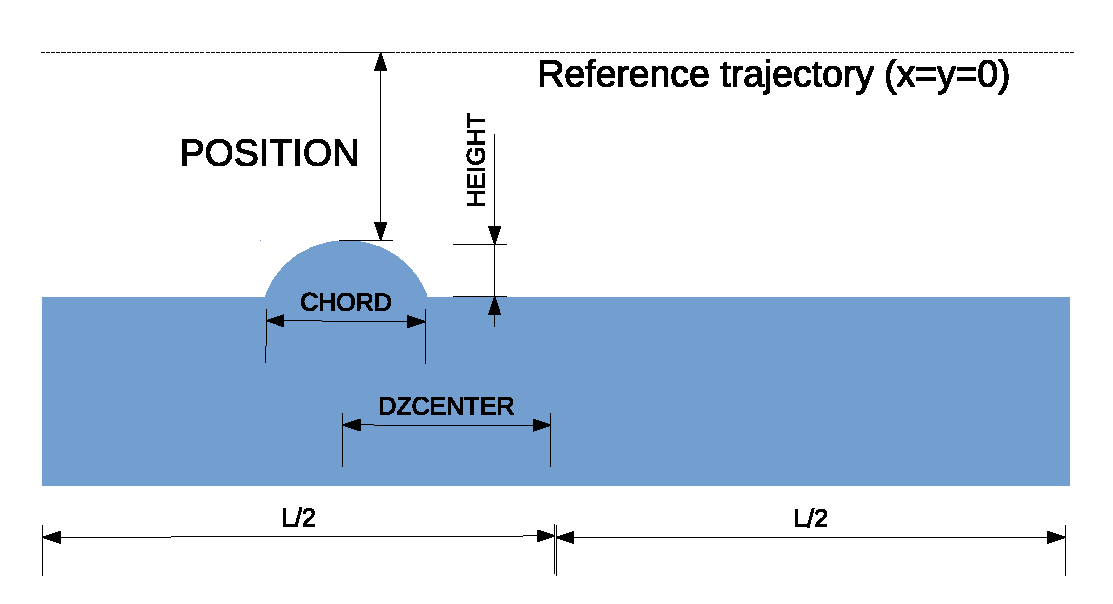
\includegraphics[width=0.8\linewidth]{speedbump}
\caption{Illustration of the parameters used in specifying a speedbump.}
\label{fig:speedbump}
\end{figure}

\clearpage

\newpage
\begin{center}{\Large\verb|SREFFECTS|}\end{center}
\subsection{SREFFECTS---Lumped simulation of synchrotron radiation effects (damping and quantum excitation) for rings.}
Lumped simulation of synchrotron radiation effects (damping and quantum excitation) for rings.
\\
Parallel capable? : yes\\
GPU capable? : no\\
Back-tracking capable? : no\\
\begin{tabular}{|l|l|l|l|p{\descwidth}|} \hline
Parameter Name & Units & Type & Default & Description \\ \hline 
JX &  & double &   1 & x damping partition number  \\ \hline 
JY &  & double &   1 & y damping partition number  \\ \hline 
JDELTA &  & double &   2 & momentum damping partition number  \\ \hline 
EXREF & $m$ & double &  0.0 & reference equilibrium x emittance  \\ \hline 
EYREF & $m$ & double &  0.0 & reference equilibrium y emittance  \\ \hline 
SDELTAREF &  & double &  0.0 & reference equilibrium fractional momentum spread  \\ \hline 
DDELTAREF &  & double &  0.0 & reference fractional momentum change per turn due to SR (negative value)  \\ \hline 
PREF & $m_{e}c$ & double &  0.0 & reference momentum (to which other reference values pertain)  \\ \hline 
COUPLING &  & double &  0.0 & x-y coupling  \\ \hline 
FRACTION &  & double &   1 & fraction of implied SR effect to simulate with each instance  \\ \hline 
DAMPING &  & long &   1               & include damping, less rf effects?  \\ \hline 
QEXCITATION &  & long &   1               & include quantum excitation?  \\ \hline 
LOSSES &  & long &   1               & include average losses?  \\ \hline 
CUTOFF &  & double &   100 & cutoff (in sigmas) for gaussian random numbers  \\ \hline 
INCLUDE\_OFFSETS &  & long &   1               & include orbit offsets in tracking (see below)?  \\ \hline 
GROUP &  & string & NULL & Optionally used to assign an element to a group, with a user-defined name.  Group names will appear in the parameter output file in the column ElementGroup  \\ \hline 
\end{tabular}

\vspace*{0.5in}
This element allows simulation of synchrotron radiation effects in a
lumped fashion for quick, approximate results.  There are two ways to
set up the element: explicit initialization or automatic
initialization.  

In explicit initialization, the user supplies the quantities {\tt
EXREF}, {\tt EYREF}, {\tt SDELTAREF}, {\tt DDELTAREF}, and {\tt
PREF}.  These are, respectively, the reference values for the x-plane
emittance, y-plane emittance, fractional momentum spread, energy loss
per turn, and momentum.  The first four values pertain to the
reference momentum.  {\tt JX}, {\tt JY}, and {\tt JDELTA} may also
be given, although the defaults work for typical lattices.

In automatic initialization, the user turns on the radiation integral
feature in {\tt twiss\_output}, causing {\tt elegant} to automatically
compute the above quantities.  This will occur only if {\tt PREF=0}.
The {\tt COUPLING} parameter can be used to change the partitioning of
quantum excitation between the horizontal and vertical planes.

N.B.: Computation of Twiss parameters does not fully include the
effects of synchrotron radiation losses when these are imposed using
{\tt SREFFECTS} elements.  If {\tt PREF=0} (automatic initialization),
these effects are completely missing.  If {\tt PREF} is non-zero, then
{\tt elegant} will use the {\tt DDELTAREF} parameter to compute the
energy offset from the element, and thus its effect on the beam
trajectory.




\newpage
\begin{center}{\Large\verb|STRAY|}\end{center}
\subsection{STRAY---A stray field element with local and global components.  Global components are defined relative to the initial beamline direction.}
A stray field element with local and global components.  Global components are defined relative to the initial beamline direction.
\\
Parallel capable? : yes\\
GPU capable? : no\\
Back-tracking capable? : no\\
\begin{tabular}{|l|l|l|l|p{\descwidth}|} \hline
Parameter Name & Units & Type & Default & Description \\ \hline 
L & $M$ & double &  0.0 & length  \\ \hline 
LBX & $T$ & double &  0.0 & local Bx  \\ \hline 
LBY & $T$ & double &  0.0 & local By  \\ \hline 
GBX & $T$ & double &  0.0 & global Bx  \\ \hline 
GBY & $T$ & double &  0.0 & global By  \\ \hline 
GBZ & $T$ & double &  0.0 & global Bz  \\ \hline 
ORDER &  & long &  \verb|0| & matrix order  \\ \hline 
GROUP &  & string & NULL & Optionally used to assign an element to a group, with a user-defined name.  Group names will appear in the parameter output file in the column ElementGroup  \\ \hline 
\end{tabular}

\vspace*{0.5in}
This element simulates stray fields.  These fields are considered
perturbations, in that they change the trajectory (or orbit), but not
the floor coordinates.  Local stray fields ({\tt LBX} and {\tt LBY})
are referenced to the local coordinate system.  Global stray fields
({\tt GBX}, {\tt GBY}, {\tt GBZ}) are referenced to the global
coordinate system, which coincides with the local coordinate system
only at the start of the beamline (unless there is no bending, in
which case the two systems are identical).


\newpage
\begin{center}{\Large\verb|TAPERAPC|}\end{center}
\subsection{TAPERAPC---A tapered aperture that is a section of a circular cylinder.}
A tapered aperture that is a section of a circular cylinder.
\\
Parallel capable? : yes\\
GPU capable? : no\\
Back-tracking capable? : no\\
\begin{tabular}{|l|l|l|l|p{\descwidth}|} \hline
Parameter Name & Units & Type & Default & Description \\ \hline 
L & $M$ & double &  0.0 & length  \\ \hline 
RSTART & $M$ & double &  0.0 & radius at the start  \\ \hline 
REND & $M$ & double &  0.0 & radius at the end  \\ \hline 
DX & $M$ & double &  0.0 & misalignment  \\ \hline 
DY & $M$ & double &  0.0 & misalignment  \\ \hline 
STICKY & $NULL$ & short &  \verb|0| & final aperture holds downstream until next TAPERAPC, TAPERAPE, TAPERAPR, or MAXAMP  \\ \hline 
GROUP &  & string & NULL & Optionally used to assign an element to a group, with a user-defined name.  Group names will appear in the parameter output file in the column ElementGroup  \\ \hline 
\end{tabular}

\newpage
\begin{center}{\Large\verb|TAPERAPE|}\end{center}
\subsection{TAPERAPE---A tapered elliptical aperture.}
A tapered elliptical aperture.
\\
Parallel capable? : yes\\
GPU capable? : no\\
Back-tracking capable? : no\\
\begin{tabular}{|l|l|l|l|p{\descwidth}|} \hline
Parameter Name & Units & Type & Default & Description \\ \hline 
L & $M$ & double &  0.0 & length  \\ \hline 
ASTART & $M$ & double &  0.0 & horizontal semi-axis at the start  \\ \hline 
AEND & $M$ & double &  0.0 & horizontal semi-axis at the end  \\ \hline 
BSTART & $M$ & double &  0.0 & vertical semi-axis at the start  \\ \hline 
BEND & $M$ & double &  0.0 & vertical semi-axis at the end  \\ \hline 
DX & $M$ & double &  0.0 & misalignment  \\ \hline 
DY & $M$ & double &  0.0 & misalignment  \\ \hline 
TILT & $RAD$ & double &  0.0 & misalignment  \\ \hline 
RESOLUTION & $M$ & double &   1e-06 & z resolution of finding intersection  \\ \hline 
XEXPONENT & $NULL$ & short &   2               & super-elliptical exponent (even number)  \\ \hline 
YEXPONENT & $NULL$ & short &   2               & super-elliptical exponent (even number)  \\ \hline 
STICKY & $NULL$ & short &  \verb|0| & final aperture holds downstream until next TAPERAPC, TAPERAPE, TAPERAPR, or MAXAMP  \\ \hline 
GROUP &  & string & NULL & Optionally used to assign an element to a group, with a user-defined name.  Group names will appear in the parameter output file in the column ElementGroup  \\ \hline 
\end{tabular}

\newpage
\begin{center}{\Large\verb|TAPERAPR|}\end{center}
\subsection{TAPERAPR---A tapered rectangular aperture.}
A tapered rectangular aperture.
\\
Parallel capable? : yes\\
GPU capable? : no\\
Back-tracking capable? : no\\
\begin{tabular}{|l|l|l|l|p{\descwidth}|} \hline
Parameter Name & Units & Type & Default & Description \\ \hline 
L & $M$ & double &  0.0 & length  \\ \hline 
XSTART & $M$ & double &  0.0 & horizontal half-aperture at the start  \\ \hline 
XEND & $M$ & double &  0.0 & horizontal half-aperture at the end  \\ \hline 
YSTART & $M$ & double &  0.0 & vertical half-aperture at the start  \\ \hline 
YEND & $M$ & double &  0.0 & vertical half-aperture at the end  \\ \hline 
DX & $M$ & double &  0.0 & misalignment  \\ \hline 
DY & $M$ & double &  0.0 & misalignment  \\ \hline 
TILT & $RAD$ & double &  0.0 & misalignment  \\ \hline 
STICKY & $NULL$ & short &  \verb|0| & final aperture holds downstream until next TAPERAPC, TAPERAPE, TAPERAPR, or MAXAMP  \\ \hline 
GROUP &  & string & NULL & Optionally used to assign an element to a group, with a user-defined name.  Group names will appear in the parameter output file in the column ElementGroup  \\ \hline 
\end{tabular}

\newpage
\begin{center}{\Large\verb|TFBDRIVER|}\end{center}
\subsection{TFBDRIVER---Driver for a turn-by-turn feedback loop}
Driver for a turn-by-turn feedback loop
\\
Parallel capable? : yes\\
GPU capable? : no\\
Back-tracking capable? : no\\
\begin{tabular}{|l|l|l|l|p{\descwidth}|} \hline
Parameter Name & Units & Type & Default & Description \\ \hline 
ID &  & STRING &   NULL            & System identifier  \\ \hline 
STRENGTH &  & double &  0.0 & Strength factor  \\ \hline 
KICK\_LIMIT &  & double &  0.0 & Limit on applied kick, nominally in radians.  \\ \hline 
FREQUENCY & $Hz$ & double &  0.0 & Resonant frequency of the unloaded kicker cavity.  \\ \hline 
DRIVE\_FREQUENCY & $Hz$ & double &  0.0 & Drive frequency. If zero, defaults to resonant frequency of the loaded cavity.  \\ \hline 
CLOCK\_FREQUENCY & $Hz$ & double &  0.0 & Clock frequency used for timing of the changes to generator current. Typically the rf or bunch frequency is used.  \\ \hline 
CLOCK\_OFFSET & $s$ & double &  0.0 & Offset of the generator current change relative to clock tick. Clock tick is nominally aligned to the bunch center.  \\ \hline 
PHASE & $Deg$ & double &  0.0 & Phase of the applied voltage relative to the bunch center, with 0 being on-crest.  \\ \hline 
RAOVERQ & $Ohm$ & double &  0.0 & Shunt impedance, Ra/Q=V\^2/(P*Q).  \\ \hline 
QLOADED &  & double &  0.0 & Loaded Q of the cavity.  \\ \hline 
OUTPUT\_FILE &  & STRING &   NULL            & File for logging filter output and driver output  \\ \hline 
GAIN\_FACTOR\_FILE &  & STRING &   NULL            & File providing gain factors for individual bunches.  \\ \hline 
GAIN\_FACTOR\_COLUMN &  & STRING &   NULL            & Column from GAIN\_FACTOR\_FILE containing gain factors.  \\ \hline 
DELAY &  & long &  \verb|0| & Delay (in turns)  \\ \hline 
A0 &  & double &   1 & Filter coefficient  \\ \hline 
A1 &  & double &  0.0 & Filter coefficient  \\ \hline 
A2 &  & double &  0.0 & Filter coefficient  \\ \hline 
A3 &  & double &  0.0 & Filter coefficient  \\ \hline 
\end{tabular}

\newpage
\begin{center}{\Large\verb|TFBDRIVER| continued}\end{center}
Driver for a turn-by-turn feedback loop
\\
\begin{tabular}{|l|l|l|l|p{\descwidth}|} \hline
Parameter Name & Units & Type & Default & Description \\ \hline 
A4 &  & double &  0.0 & Filter coefficient  \\ \hline 
A5 &  & double &  0.0 & Filter coefficient  \\ \hline 
A6 &  & double &  0.0 & Filter coefficient  \\ \hline 
A7 &  & double &  0.0 & Filter coefficient  \\ \hline 
A8 &  & double &  0.0 & Filter coefficient  \\ \hline 
A9 &  & double &  0.0 & Filter coefficient  \\ \hline 
A10 &  & double &  0.0 & Filter coefficient  \\ \hline 
A11 &  & double &  0.0 & Filter coefficient  \\ \hline 
A12 &  & double &  0.0 & Filter coefficient  \\ \hline 
A13 &  & double &  0.0 & Filter coefficient  \\ \hline 
A14 &  & double &  0.0 & Filter coefficient  \\ \hline 
A15 &  & double &  0.0 & Filter coefficient  \\ \hline 
A16 &  & double &  0.0 & Filter coefficient  \\ \hline 
A17 &  & double &  0.0 & Filter coefficient  \\ \hline 
A18 &  & double &  0.0 & Filter coefficient  \\ \hline 
A19 &  & double &  0.0 & Filter coefficient  \\ \hline 
A20 &  & double &  0.0 & Filter coefficient  \\ \hline 
A21 &  & double &  0.0 & Filter coefficient  \\ \hline 
A22 &  & double &  0.0 & Filter coefficient  \\ \hline 
A23 &  & double &  0.0 & Filter coefficient  \\ \hline 
A24 &  & double &  0.0 & Filter coefficient  \\ \hline 
A25 &  & double &  0.0 & Filter coefficient  \\ \hline 
A26 &  & double &  0.0 & Filter coefficient  \\ \hline 
A27 &  & double &  0.0 & Filter coefficient  \\ \hline 
A28 &  & double &  0.0 & Filter coefficient  \\ \hline 
A29 &  & double &  0.0 & Filter coefficient  \\ \hline 
UPDATE\_INTERVAL &  & long &  \verb|0| & Interval in units of pickup update interval for sampling pickup data and updating filter output.  \\ \hline 
OUTPUT\_INTERVAL &  & long &   1024            & Number of samples to buffer between writing output file updates.  \\ \hline 
START\_PASS &  & long &   -1              & If positive, first pass on which to drive beam.  \\ \hline 
END\_PASS &  & long &   -1              & If positive, last pass on which to drive beam.  \\ \hline 
\end{tabular}

\newpage
\begin{center}{\Large\verb|TFBDRIVER| continued}\end{center}
Driver for a turn-by-turn feedback loop
\\
\begin{tabular}{|l|l|l|l|p{\descwidth}|} \hline
Parameter Name & Units & Type & Default & Description \\ \hline 
LONGITUDINAL &  & short &  \verb|0| & If non-zero, kick is in the longituidinal plane. KICK\_LIMIT is in fractional momentum deviation.  \\ \hline 
BUNCHED\_BEAM\_MODE &  & short &   1               & If non-zero, run in bunched beam mode.  \\ \hline 
GROUP &  & string & NULL & Optionally used to assign an element to a group, with a user-defined name.  Group names will appear in the parameter output file in the column ElementGroup  \\ \hline 
\end{tabular}

\vspace*{0.5in}
This element is used together with the {\tt TFBPICKUP} element to
simulate a digital turn-by-turn feedback system.  Each {\tt TFBDRIVER}
element must have a unique identification string assigned to it using
the {\tt ID} parameter.  The same identifier must be used on a {\tt
TFBPICKUP} element.  This is the pickup from which the driver gets its
signal.  Each pickup may feed more than one driver, but a driver can
use only one pickup.

A 15-term FIR filter can be defined using the {\tt A0} through {\tt
A14} parameters.  The output of the filter is simply $\sum_{i=0}^{14}
a_i P_i$, where $P_i$ is the pickup filter output from $i$ turns ago.
The output of the filter is optionally delayed by the number of turns
given by the {\tt DELAY} parameter.

To some extent, the {\tt DELAY} is redundant.  For example, the filter
$a_0=0, a_1=1$ with a delay of 0 is equivalent to $a_0=1, a_1=0$ with
a delay of 1.  However, for long delays or delays combined with
many-term filters, the {\tt DELAY} feature must be used.

The output of the filter is multiplied by the {\tt STRENGTH} parameter
to get the kick to apply to the beam.  The {\tt KICK\_LIMIT} parameter
provides a very basic way to simulate saturation of the kicker output.

The plane that the \verb|TFBDRIVER| kicks is determined by the 
\verb|PLANE| parameter on the corresponding \verb|TFBPICKUP| element, and
additionally by the \verb|LONGITUDINAL| parameter, as described in 
Table \ref{tab:tfbdriver}

\begin{table}[htb]
\begin{tabular}{llll}
\hline
\verb|TFBPICKUP| & \verb|TFBDRIVER| & coordinate & note \\
\verb|PLANE| & \verb|LONGITUDINAL| & kicked & \\
\hline
x & 0 & $x^\prime$ & \\
x & 1 & $\delta$ & pickup should have $\eta_x\neq 0$ \\
y & 0 & $y\prime$ & \\
y & 1 & $\delta$ & pickup should have $\eta_y\neq 0$ \\
delta & 0 & - & invalid \\
delta & 1 & $\delta$ & \\
\hline
\end{tabular}
\caption{Correspondence between {\tt PLANE} parameter of {\tt TFBPICKUP}, {\tt LONGITUDINAL} parameter of {\tt TFBDRIVER}, and action of feedback loop.}
\label{tab:tfbdriver}
\end{table}

See Section 7.2.14 of {\em Handbook of Accelerator Physics and Engineering}
(Chao and Tigner, eds.) for a discussion of feedback systems.

\newpage
\begin{center}{\Large\verb|TFBPICKUP|}\end{center}
\subsection{TFBPICKUP---Pickup for a turn-by-turn feedback loop}
Pickup for a turn-by-turn feedback loop
\\
Parallel capable? : yes\\
GPU capable? : no\\
Back-tracking capable? : no\\
\begin{tabular}{|l|l|l|l|p{\descwidth}|} \hline
Parameter Name & Units & Type & Default & Description \\ \hline 
ID &  & STRING &   NULL            & System identifier  \\ \hline 
PLANE &  & STRING &   x               & "x", "y", "delta", or "phase"  \\ \hline 
RMS\_NOISE & $M$ & double &  0.0 & RMS noise to add to position readings.  \\ \hline 
A0 &  & double &  0.0 & Filter coefficient  \\ \hline 
A1 &  & double &  0.0 & Filter coefficient  \\ \hline 
A2 &  & double &  0.0 & Filter coefficient  \\ \hline 
A3 &  & double &  0.0 & Filter coefficient  \\ \hline 
A4 &  & double &  0.0 & Filter coefficient  \\ \hline 
A5 &  & double &  0.0 & Filter coefficient  \\ \hline 
A6 &  & double &  0.0 & Filter coefficient  \\ \hline 
A7 &  & double &  0.0 & Filter coefficient  \\ \hline 
A8 &  & double &  0.0 & Filter coefficient  \\ \hline 
A9 &  & double &  0.0 & Filter coefficient  \\ \hline 
A10 &  & double &  0.0 & Filter coefficient  \\ \hline 
A11 &  & double &  0.0 & Filter coefficient  \\ \hline 
A12 &  & double &  0.0 & Filter coefficient  \\ \hline 
A13 &  & double &  0.0 & Filter coefficient  \\ \hline 
A14 &  & double &  0.0 & Filter coefficient  \\ \hline 
A15 &  & double &  0.0 & Filter coefficient  \\ \hline 
A16 &  & double &  0.0 & Filter coefficient  \\ \hline 
A17 &  & double &  0.0 & Filter coefficient  \\ \hline 
A18 &  & double &  0.0 & Filter coefficient  \\ \hline 
A19 &  & double &  0.0 & Filter coefficient  \\ \hline 
A20 &  & double &  0.0 & Filter coefficient  \\ \hline 
A21 &  & double &  0.0 & Filter coefficient  \\ \hline 
A22 &  & double &  0.0 & Filter coefficient  \\ \hline 
A23 &  & double &  0.0 & Filter coefficient  \\ \hline 
A24 &  & double &  0.0 & Filter coefficient  \\ \hline 
A25 &  & double &  0.0 & Filter coefficient  \\ \hline 
A26 &  & double &  0.0 & Filter coefficient  \\ \hline 
A27 &  & double &  0.0 & Filter coefficient  \\ \hline 
A28 &  & double &  0.0 & Filter coefficient  \\ \hline 
A29 &  & double &  0.0 & Filter coefficient  \\ \hline 
UPDATE\_INTERVAL &  & long &  \verb|0| & Interval in turns for sampling data and updating filter output.  \\ \hline 
\end{tabular}

\newpage
\begin{center}{\Large\verb|TFBPICKUP| continued}\end{center}
Pickup for a turn-by-turn feedback loop
\\
\begin{tabular}{|l|l|l|l|p{\descwidth}|} \hline
Parameter Name & Units & Type & Default & Description \\ \hline 
START\_PASS &  & long &   -1              & If positive, first pass on which to perform computations.  \\ \hline 
END\_PASS &  & long &   -1              & If positive, last pass on which to perform computations.  \\ \hline 
REFERENCE\_FREQUENCY &  & double &  0.0 & Reference frequency for computing phase offsets.  \\ \hline 
DX & $M$ & double &  0.0 & Horizontal offset (subtracted from pickup signal).  \\ \hline 
DY & $M$ & double &  0.0 & Vertical offset (subtracted from pickup signal)  \\ \hline 
BUNCHED\_BEAM\_MODE &  & short &   1               & If non-zero, run in bunched beam mode.  \\ \hline 
GROUP &  & string & NULL & Optionally used to assign an element to a group, with a user-defined name.  Group names will appear in the parameter output file in the column ElementGroup  \\ \hline 
\end{tabular}

\vspace*{0.5in}
This element is used together with the {\tt TFBDRIVER} element to
simulate a digital turn-by-turn feedback system.  Each {\tt TFBPICKUP}
element must have a unique identification string assigned to it using
the {\tt ID} parameter.  This is used to identify which drivers get
signals from the pickup.

A 15-term FIR filter can be defined using the {\tt A0} through {\tt
A14} parameters.  The input to the filter is the turn-by-turn beam
centroid at the pickup location.  The output of the filter is simply
$\sum_{i=0}^{14} a_i C_i$, where $C_i$ is the centroid from $i*U$ turns
ago, where $U$ is the value specified by the \verb|UPDATE_INTERVAL| parameter.
Note that $\sum_{i=0}^{14} a_i$ should generally be zero. Otherwise, the
system will attempt to correct the DC orbit.  The output of the filter
is the input to the driver element(s).

The \verb|PLANE| parameter can take three values: ``x'', ``y'', and ``delta'', specifying
what centroid property of the beam is measured by the pickup. The ``delta''-mode pickup
is nonphysical, but could have applications to cases where is not convenient to put a 
pickup in a high-dispersion area.

See Section 7.2.14 of {\em Handbook of Accelerator Physics and Engineering}
(Chao and Tigner, eds.) for a discussion of feedback systems.

\newpage
\begin{center}{\Large\verb|TMCF|}\end{center}
\subsection{TMCF---A numerically-integrated accelerating TM RF cavity with spatially-constant fields.}
A numerically-integrated accelerating TM RF cavity with spatially-constant fields.
\\
Parallel capable? : yes\\
GPU capable? : no\\
Back-tracking capable? : no\\
\begin{tabular}{|l|l|l|l|p{\descwidth}|} \hline
Parameter Name & Units & Type & Default & Description \\ \hline 
L & $M$ & double &  0.0 & length  \\ \hline 
FREQUENCY & $HZ$ & double &   2856000000 & frequency  \\ \hline 
PHASE & $S$ & double &  0.0 & phase  \\ \hline 
TIME\_OFFSET & $S$ & double &  0.0 & time offset (adds to phase)  \\ \hline 
RADIAL\_OFFSET & $M$ & double &   1 & not recommended  \\ \hline 
TILT & $RAD$ & double &  0.0 & rotation about longitudinal axis  \\ \hline 
ER & $V$ & double &  0.0 & radial electric field  \\ \hline 
BPHI & $T$ & double &  0.0 & azimuthal magnetic field  \\ \hline 
EZ & $V$ & double &  0.0 & longitudinal electric field  \\ \hline 
ACCURACY &  & double &   0.0001 & integration accuracy  \\ \hline 
X\_MAX & $M$ & double &  0.0 & x half-aperture  \\ \hline 
Y\_MAX & $M$ & double &  0.0 & y half-aperture  \\ \hline 
DX & $M$ & double &  0.0 & misalignment  \\ \hline 
DY & $M$ & double &  0.0 & misalignment  \\ \hline 
PHASE\_REFERENCE &  & long &  \verb|0| & phase reference number (to link with other time-dependent elements)  \\ \hline 
N\_STEPS &  & long &   100             & number of steps (for nonadaptive integration)  \\ \hline 
METHOD & $ $ & STRING &   runge-kutta     & integration method (runge-kutta, bulirsch-stoer, non-adaptive runge-kutta, modified midpoint)  \\ \hline 
FIDUCIAL &  & STRING &   t,median        & \{t$|$p\},\{median$|$min$|$max$|$ave$|$first$|$light\} (e.g., "t,median")  \\ \hline 
GROUP &  & string & NULL & Optionally used to assign an element to a group, with a user-defined name.  Group names will appear in the parameter output file in the column ElementGroup  \\ \hline 
\end{tabular}

\newpage
\begin{center}{\Large\verb|TRCOUNT|}\end{center}
\subsection{TRCOUNT---An element that defines the point from which transmission calculations are made.}
An element that defines the point from which transmission calculations are made.
\\
Parallel capable? : no\\
GPU capable? : no\\
Back-tracking capable? : no\\
\begin{tabular}{|l|l|l|l|p{\descwidth}|} \hline
Parameter Name & Units & Type & Default & Description \\ \hline 
DUMMY &  & long &  \verb|0| & \\ \hline 
GROUP &  & string & NULL & Optionally used to assign an element to a group, with a user-defined name.  Group names will appear in the parameter output file in the column ElementGroup  \\ \hline 
\end{tabular}

\newpage
\begin{center}{\Large\verb|TRFMODE|}\end{center}
\subsection{TRFMODE---A simulation of a beam-driven TM dipole mode of an RF cavity.}
A simulation of a beam-driven TM dipole mode of an RF cavity.
\\
Parallel capable? : yes\\
GPU capable? : no\\
Back-tracking capable? : no\\
\begin{tabular}{|l|l|l|l|p{\descwidth}|} \hline
Parameter Name & Units & Type & Default & Description \\ \hline 
RA & $Ohm/m$ & double &  0.0 & shunt impedance, Ra=V\^2/P  \\ \hline 
RS & $Ohm/m$ & double &  0.0 & shunt impedance (Rs=Ra/2)  \\ \hline 
Q &  & double &  0.0 & cavity Q  \\ \hline 
FREQ & $Hz$ & double &  0.0 & frequency  \\ \hline 
CHARGE & $C$ & double &  0.0 & beam charge (or use CHARGE element)  \\ \hline 
BETA &  & double &  0.0 & normalized load impedance  \\ \hline 
BIN\_SIZE & $S$ & double &  0.0 & bin size for current histogram (use 0 for autosize)  \\ \hline 
N\_BINS &  & long &   20              & number of bins for current histogram  \\ \hline 
INTERPOLATE &  & long &  \verb|0| & if non-zero, interpolate voltage within bins  \\ \hline 
PLANE &  & STRING &   both            & x, y, or both  \\ \hline 
SAMPLE\_INTERVAL &  & long &   1               & passes between output to RECORD file  \\ \hline 
PER\_PARTICLE\_OUTPUT &  & long &  \verb|0| & If non-zero, then in BINLESS mode, provides per-particle output of RECORD data.  \\ \hline 
RECORD &  & STRING &   NULL            & output file for cavity data  \\ \hline 
SINGLE\_PASS &  & long &  \verb|0| & if nonzero, don't accumulate field from pass to pass  \\ \hline 
RIGID\_UNTIL\_PASS &  & long &  \verb|0| & don't affect the beam until this pass  \\ \hline 
DX & $M$ & double &  0.0 & misalignment  \\ \hline 
DY & $M$ & double &  0.0 & misalignment  \\ \hline 
XFACTOR &  & double &   1 & factor by which to multiply shunt impedances  \\ \hline 
YFACTOR &  & double &   1 & factor by which to multiply shunt impedances  \\ \hline 
RAMP\_PASSES &  & long &  \verb|0| & Number of passes over which to linearly ramp up the impedance to full strength.  \\ \hline 
BINLESS &  & long &  \verb|0| & If nonzero, use algorithm that doesn't requiring binning.  Best for few particles, widely spaced.  \\ \hline 
\end{tabular}

\newpage
\begin{center}{\Large\verb|TRFMODE| continued}\end{center}
A simulation of a beam-driven TM dipole mode of an RF cavity.
\\
\begin{tabular}{|l|l|l|l|p{\descwidth}|} \hline
Parameter Name & Units & Type & Default & Description \\ \hline 
RESET\_FOR\_EACH\_STEP &  & long &   1               & If nonzero, voltage and phase are reset for each simulation step.  \\ \hline 
LONG\_RANGE\_ONLY &  & long &  \verb|0| & If nonzero, induced voltage from present turn does not affect bunch. Short range wake should be included via TRWAKE or ZTRANSVERSE element.  \\ \hline 
N\_CAVITIES &  & long &   1               & effect is multiplied by this number, simulating N identical cavities  \\ \hline 
BUNCHED\_BEAM\_MODE &  & long &   1               & If non-zero, then do calculations bunch-by-bunch.  \\ \hline 
GROUP &  & string & NULL & Optionally used to assign an element to a group, with a user-defined name.  Group names will appear in the parameter output file in the column ElementGroup  \\ \hline 
\end{tabular}

\vspace*{0.5in}
This element simulates a beam-driven dipole mode cavity using the fundamental theorem of beam loading and phasor rotation.

Normally, the field dumped in the cavity by one particle affects trailing particles in the same turn.
However, if one is also using a \verb|TRWAKE| or \verb|ZTRANSVSE| element to simulate the short-range wake of the cavity, this would be double-counting.
In that case, one can use \verb|LONG_RANGE_ONLY=1| to suppress the same-turn effects of the \verb|RFMODE| element.

\newpage
\begin{center}{\Large\verb|TRWAKE|}\end{center}
\subsection{TRWAKE---Transverse wake specified as a function of time lag behind the particle.}
Transverse wake specified as a function of time lag behind the particle.
\\
Parallel capable? : yes\\
GPU capable? : yes\\
Back-tracking capable? : yes\\
\begin{tabular}{|l|l|l|l|p{\descwidth}|} \hline
Parameter Name & Units & Type & Default & Description \\ \hline 
INPUTFILE &  & STRING &   NULL            & name of file giving Green functions  \\ \hline 
TCOLUMN &  & STRING &   NULL            & column in INPUTFILE containing time data  \\ \hline 
WXCOLUMN &  & STRING &   NULL            & column in INPUTFILE containing x Green function  \\ \hline 
WYCOLUMN &  & STRING &   NULL            & column in INPUTFILE containing y Green function  \\ \hline 
CHARGE & $C$ & double &  0.0 & beam charge (or use CHARGE element)  \\ \hline 
FACTOR &  & double &   1 & factor by which to multiply both wakes  \\ \hline 
XFACTOR &  & double &   1 & factor by which to multiply x wake  \\ \hline 
YFACTOR &  & double &   1 & factor by which to multiply y wake  \\ \hline 
N\_BINS &  & long &  \verb|0| & number of bins for current histogram  \\ \hline 
INTERPOLATE &  & long &  \verb|0| & interpolate wake?  \\ \hline 
SMOOTHING &  & long &  \verb|0| & Use Savitzky-Golay filter to smooth current histogram?  \\ \hline 
SG\_HALFWIDTH &  & long &   4               & Savitzky-Golay filter half-width for smoothing  \\ \hline 
SG\_ORDER &  & long &   1               & Savitzky-Golay filter order for smoothing  \\ \hline 
DX & $M$ & double &  0.0 & misalignment  \\ \hline 
DY & $M$ & double &  0.0 & misalignment  \\ \hline 
TILT & $RAD$ & double &  0.0 & rotation about longitudinal axis  \\ \hline 
X\_DRIVE\_EXPONENT &  & long &   1               & Exponent applied to x coordinates of drive particles  \\ \hline 
Y\_DRIVE\_EXPONENT &  & long &   1               & Exponent applied to y coordinates of drive particles  \\ \hline 
X\_PROBE\_EXPONENT &  & long &  \verb|0| & Exponent applied to x coordinates of probe particles  \\ \hline 
Y\_PROBE\_EXPONENT &  & long &  \verb|0| & Exponent applied to y coordinates of probe particles  \\ \hline 
\end{tabular}

\newpage
\begin{center}{\Large\verb|TRWAKE| continued}\end{center}
Transverse wake specified as a function of time lag behind the particle.
\\
\begin{tabular}{|l|l|l|l|p{\descwidth}|} \hline
Parameter Name & Units & Type & Default & Description \\ \hline 
RAMP\_PASSES &  & long &  \verb|0| & Number of passes over which to linearly ramp up the wake to full strength.  \\ \hline 
BUNCHED\_BEAM\_MODE &  & long &   1               & If non-zero, then do calculations bunch-by-bunch.  \\ \hline 
ACAUSAL\_ALLOWED &  & long &  \verb|0| & If non-zero, then an acausal wake is allowed.  \\ \hline 
GROUP &  & string & NULL & Optionally used to assign an element to a group, with a user-defined name.  Group names will appear in the parameter output file in the column ElementGroup  \\ \hline 
\end{tabular}

\vspace*{0.5in}
The input file for this element gives the transverse-wake Green
functions, $W_x(t)$ and $W_y(t)$, versus time behind the particle. The
units of the wakes are V/C/m, so this element simulates the integrated
wake of some structure (e.g., a cell or series of cells).  If you
have, for example, the wake for a cell and you need the wake for N
cells, then you may use the {\tt FACTOR} parameter to make the
appropriate multiplication.  The values of the time coordinate should
begin at 0 and be equi-spaced.  A positive value of time represents
the distance behind the exciting particle.   Time values must be equally
spaced.

The sign convention for $W_q$ ($q$ being $x$ or $y$) is as follows: a
particle with $q>0$ will impart a positive kick ($\Delta q^\prime >
0$) to a trailing particle following $t$ seconds behind if $W_q(t)>0$.
A physical wake function should be zero at $t=0$ and also be initially
positive as $t$ increases from 0.

Use of the {\tt CHARGE} parameter on the {\tt TRWAKE} element is
disparaged.  It is preferred to use the {\tt CHARGE} element as part
of your beamline to define the charge.  

Setting the {\tt N\_BINS} paramater to 0 is recommended.  This results
in auto-scaling of the number of bins to accomodate the beam.  The bin
size is fixed by the spacing of the time points in the wake.

The default degree of smoothing ({\tt SG\_HALFWIDTH=4}) may be excessive.
It is suggested that users vary this parameter to verify that results
are reliable if smoothing is employed ({\tt SMOOTHING=1}).

The {\tt XFACTOR} and {\tt YFACTOR} parameters can be used to adjust
the strength of the wakes if the location at which you place the {\tt
TRWAKE} element has different beta functions than the location at
which the object that causes the wake actually resides.  

The {\tt XPOWER} and {\tt YPOWER} parameters can be used to change the
dependence of the wake on the x and y coordinates, respectively, of
the particles.  Normally, {\tt XPOWER=1} and {\tt YPOWER=1}.  This is
an ordinary dipole wake in a (supposedly) symmetric chamber.  If you
have an asymmetric chamber, then you will have a transverse wake kick
even if the beam is centered.  This part of the transverse wake is
described with {\tt XPOWER=0} and {\tt YPOWER=0}.  (Of course, you'll
need a 3-D wake code like GdfidL or MAFIA to compute this wake.)

If {\tt XPOWER=0} or {\tt YPOWER=0}, the units for the x or y wake
(respectively) must be $V/C$.  A negative value of the wake
corresponds to a kick toward negative x (or y).  

\newpage
\begin{center}{\Large\verb|TSCATTER|}\end{center}
\subsection{TSCATTER---An element to simulate Touschek scattering.}
An element to simulate Touschek scattering.
\\
Parallel capable? : yes\\
GPU capable? : no\\
Back-tracking capable? : no\\
\begin{tabular}{|l|l|l|l|p{\descwidth}|} \hline
Parameter Name & Units & Type & Default & Description \\ \hline 
DUMMY &  & long &  \verb|0| & \\ \hline 
GROUP &  & string & NULL & Optionally used to assign an element to a group, with a user-defined name.  Group names will appear in the parameter output file in the column ElementGroup  \\ \hline 
\end{tabular}

\newpage
\begin{center}{\Large\verb|TUBEND|}\end{center}
\subsection{TUBEND---A special rectangular bend element for top-up backtracking.}
A special rectangular bend element for top-up backtracking.
\\
Parallel capable? : yes\\
GPU capable? : no\\
Back-tracking capable? : no\\
\begin{tabular}{|l|l|l|l|p{\descwidth}|} \hline
Parameter Name & Units & Type & Default & Description \\ \hline 
L & $M$ & double &  0.0 & arc length  \\ \hline 
ANGLE & $RAD$ & double &  0.0 & bend angle  \\ \hline 
FSE &  & double &  0.0 & fractional strength error  \\ \hline 
OFFSET &  & double &  0.0 & horizontal offset of magnet center from arc center  \\ \hline 
MAGNET\_WIDTH &  & double &  0.0 & horizontal width of the magnet pole  \\ \hline 
MAGNET\_ANGLE &  & double &  0.0 & angle that the magnet was designed for  \\ \hline 
GROUP &  & string & NULL & Optionally used to assign an element to a group, with a user-defined name.  Group names will appear in the parameter output file in the column ElementGroup  \\ \hline 
\end{tabular}

\newpage
\begin{center}{\Large\verb|TWISS|}\end{center}
\subsection{TWISS---Sets Twiss parameter values.}
Sets Twiss parameter values.
\\
Parallel capable? : yes\\
GPU capable? : no\\
Back-tracking capable? : no\\
\begin{tabular}{|l|l|l|l|p{\descwidth}|} \hline
Parameter Name & Units & Type & Default & Description \\ \hline 
BETAX & $M$ & double &   1 & horizontal beta function  \\ \hline 
ALPHAX &  & double &  0.0 & horizontal alpha function  \\ \hline 
ETAX & $M$ & double &  0.0 & horizontal eta function  \\ \hline 
ETAXP &  & double &  0.0 & slope of horizontal eta function  \\ \hline 
BETAY & $M$ & double &   1 & vertical beta function  \\ \hline 
ALPHAY &  & double &  0.0 & vertical alpha function  \\ \hline 
ETAY & $M$ & double &  0.0 & vertical eta function  \\ \hline 
ETAYP &  & double &  0.0 & slope of vertical eta function  \\ \hline 
FROM\_BEAM &  & short &  \verb|0| & compute transformation from tracked beam properties instead of Twiss parameters?  \\ \hline 
FROM\_0VALUES &  & short &  \verb|0| & if non-zero, transformation is from the "0" values provided in the element definition  \\ \hline 
COMPUTE\_ONCE &  & short &  \verb|0| & compute transformation only for first beam or lattice functions?  \\ \hline 
APPLY\_ONCE &  & short &   1               & apply correction only on first pass through for each beam?  \\ \hline 
VERBOSE &  & short &  \verb|0| & if non-zero, print extra information about transformations  \\ \hline 
DISABLE &  & short &  \verb|0| & if non-zero, element is ignored  \\ \hline 
BETAX0 & $M$ & double &   1 & initial horizontal beta function (if FROM\_0VALUES nonzero)  \\ \hline 
ALPHAX0 &  & double &  0.0 & initial horizontal alpha function (if FROM\_0VALUES nonzero)  \\ \hline 
ETAX0 & $M$ & double &  0.0 & initial horizontal eta function (if FROM\_0VALUES nonzero)  \\ \hline 
\end{tabular}

\newpage
\begin{center}{\Large\verb|TWISS| continued}\end{center}
Sets Twiss parameter values.
\\
\begin{tabular}{|l|l|l|l|p{\descwidth}|} \hline
Parameter Name & Units & Type & Default & Description \\ \hline 
ETAXP0 &  & double &  0.0 & initial slope of horizontal eta function (if FROM\_0VALUES nonzero)  \\ \hline 
BETAY0 & $M$ & double &   1 & initial vertical beta function (if FROM\_0VALUES nonzero)  \\ \hline 
ALPHAY0 &  & double &  0.0 & initial vertical alpha function (if FROM\_0VALUES nonzero)  \\ \hline 
ETAY0 & $M$ & double &  0.0 & initial vertical eta function (if FROM\_0VALUES nonzero)  \\ \hline 
ETAYP0 &  & double &  0.0 & initial slope of vertical eta function (if FROM\_0VALUES nonzero)  \\ \hline 
GROUP &  & string & NULL & Optionally used to assign an element to a group, with a user-defined name.  Group names will appear in the parameter output file in the column ElementGroup  \\ \hline 
\end{tabular}

\vspace*{0.5in}
This elements allows transformation of the twiss parameters of 
a beam with a first-order matrix.  The matrix is computed in 
various ways based on initial and final twiss parameters.  Depending on 
how you set it up, the final twiss parameters for your
beam may not be the twiss parameters you specify.  

The twiss parameter values \verb|BETAX|, \verb|BETAY|, etc. specified in the
element definition specify the target values of the transformation.
To completely specify the transformation, one must know the initial
values as well.  

{\bf Lattice-Function-Based Transformation}

If \verb|FROM_BEAM| is zero, which is the default, then the initial
values are taken from the incoming lattice functions computed by
\verb|twiss_output|.  This provides a way to transform the lattice
functions between two parts of a transport line without designing
intervening optics.  A beam that is matched at the beginning of the
transport line will remain matched.  A beam that is mismatched at the
beginning of the transport line {\em will not} be matched after
the \verb|TWISS| element.

By default, each time the twiss parameters are recomputed, the
transformation is updated to maintain the desired lattice functions at
the exit of the \verb|TWISS| element. Setting \verb|COMPUTE_ONCE| to a
non-zero value specifies that {\tt elegant} should compute the
transformation matrix only once, i.e., for the first set of computed
lattice functions.

By default, the transformation is applied to the beam only the first
time it passes the element.  Setting \verb|APPLY_ONCE| to a zero
will result in application of the transformation at each pass.

{\bf Beam-Ellipse-Based Transformation}

If \verb|FROM_BEAM| is non-zero, the the initial values for the transformation
are computed from a beam.  This provides a way to transform the beam ellipse
to the desired twiss parameters irrespective of the lattice.  The results
from \verb|twiss_output| will not necessarily be matched downstream of this
element.  Only if the beam ellipse and lattice ellipse are the same will this
occur.

By default, each time a new beam is generated, the transformation will
be updated to maintain the desired beam ellipse at the exit of the
\verb|TWISS| element.  Setting \verb|COMPUTE_ONCE| to a non-zero value
specifies that {\tt elegant} should compute the transformation matrix
only once, i.e., for the first beam it sees.

By default, the transformation is applied to the beam only the first
time it passes the element.  Setting \verb|APPLY_ONCE| to a zero
will result in application of the transformation at each pass.  This
would make sense, for example, if the \verb|TWISS| element was
filling in for a section of a ring.  It wouldn't make sense if
the \verb|TWISS| element was being used to match the beam from
a transport line to a ring.


\newpage
\begin{center}{\Large\verb|TWLA|}\end{center}
\subsection{TWLA---A numerically-integrated first-space-harmonic traveling-wave linear accelerator.}
A numerically-integrated first-space-harmonic traveling-wave linear accelerator.
\\
Parallel capable? : yes\\
GPU capable? : no\\
Back-tracking capable? : no\\
\begin{tabular}{|l|l|l|l|p{\descwidth}|} \hline
Parameter Name & Units & Type & Default & Description \\ \hline 
L & $M$ & double &  0.0 & length  \\ \hline 
FREQUENCY & $HZ$ & double &   2856000000 & frequency  \\ \hline 
PHASE & $RAD$ & double &  0.0 & phase  \\ \hline 
TIME\_OFFSET & $S$ & double &  0.0 & time offset (adds to phase)  \\ \hline 
EZ & $V/M$ & double &  0.0 & electric field  \\ \hline 
B\_SOLENOID & $T$ & double &  0.0 & solenoid field  \\ \hline 
ACCURACY &  & double &   0.0001 & integration accuracy  \\ \hline 
X\_MAX & $M$ & double &  0.0 & x half-aperture  \\ \hline 
Y\_MAX & $M$ & double &  0.0 & y half-aperture  \\ \hline 
DX & $M$ & double &  0.0 & misalignment  \\ \hline 
DY & $M$ & double &  0.0 & misalignment  \\ \hline 
BETA\_WAVE &  & double &   1 & (phase velocity)/c  \\ \hline 
ALPHA & $1/M$ & double &  0.0 & field attenuation factor  \\ \hline 
PHASE\_REFERENCE &  & long &  \verb|0| & phase reference number (to link with other time-dependent elements)  \\ \hline 
N\_STEPS &  & long &   100             & number of steps (for nonadaptive integration)  \\ \hline 
FOCUSSING &  & long &   1               & include focusing effects?  \\ \hline 
METHOD & $ $ & STRING &   runge-kutta     & integration method (runge-kutta, bulirsch-stoer, non-adaptive runge-kutta, modified midpoint)  \\ \hline 
FIDUCIAL &  & STRING &   t,median        & \{t$|$p\},\{median$|$min$|$max$|$ave$|$first$|$light\} (e.g., "t,median")  \\ \hline 
CHANGE\_P0 &  & long &  \verb|0| & does element change central momentum?  \\ \hline 
SUM\_BN2 &  & double &  0.0 & sum of squares of amplitudes of n!=0 space harmonics  \\ \hline 
GROUP &  & string & NULL & Optionally used to assign an element to a group, with a user-defined name.  Group names will appear in the parameter output file in the column ElementGroup  \\ \hline 
\end{tabular}

\newpage
\begin{center}{\Large\verb|TWMTA|}\end{center}
\subsection{TWMTA---A numerically-integrated traveling-wave muffin-tin accelerator.}
A numerically-integrated traveling-wave muffin-tin accelerator.
\\
Parallel capable? : yes\\
GPU capable? : no\\
Back-tracking capable? : no\\
\begin{tabular}{|l|l|l|l|p{\descwidth}|} \hline
Parameter Name & Units & Type & Default & Description \\ \hline 
L & $M$ & double &  0.0 & length  \\ \hline 
FREQUENCY & $HZ$ & double &   2856000000 & frequency  \\ \hline 
PHASE & $RAD$ & double &  0.0 & phase  \\ \hline 
EZ & $V/M$ & double &  0.0 & electric field  \\ \hline 
ACCURACY &  & double &   0.0001 & integration accuracy  \\ \hline 
X\_MAX & $M$ & double &  0.0 & x half-aperture  \\ \hline 
Y\_MAX & $M$ & double &  0.0 & y half-aperture  \\ \hline 
DX & $M$ & double &  0.0 & misalignment  \\ \hline 
DY & $M$ & double &  0.0 & misalignment  \\ \hline 
KX & $1/M$ & double &  0.0 & horizontal wave number  \\ \hline 
BETA\_WAVE &  & double &   1 & (phase velocity)/c  \\ \hline 
BSOL &  & double &  0.0 & solenoid field  \\ \hline 
ALPHA & $1/M$ & double &  0.0 & field attenuation factor  \\ \hline 
PHASE\_REFERENCE &  & long &  \verb|0| & phase reference number (to link with other time-dependent elements)  \\ \hline 
N\_STEPS &  & long &   100             & number of kicks  \\ \hline 
METHOD & $ $ & STRING &   runge-kutta     & integration method (runge-kutta, bulirsch-stoer, non-adaptive runge-kutta, modified midpoint)  \\ \hline 
FIDUCIAL &  & STRING &   t,median        & \{t$|$p\},\{median$|$min$|$max$|$ave$|$first$|$light\} (e.g., "t,median")  \\ \hline 
GROUP &  & string & NULL & Optionally used to assign an element to a group, with a user-defined name.  Group names will appear in the parameter output file in the column ElementGroup  \\ \hline 
\end{tabular}

\newpage
\begin{center}{\Large\verb|TWPL|}\end{center}
\subsection{TWPL---A numerically-integrated traveling-wave stripline deflector.}
A numerically-integrated traveling-wave stripline deflector.
\\
Parallel capable? : yes\\
GPU capable? : no\\
Back-tracking capable? : no\\
\begin{tabular}{|l|l|l|l|p{\descwidth}|} \hline
Parameter Name & Units & Type & Default & Description \\ \hline 
L & $M$ & double &  0.0 & length  \\ \hline 
RAMP\_TIME & $S$ & double &   1e-09 & time to ramp to full strenth  \\ \hline 
TIME\_OFFSET & $S$ & double &  0.0 & offset of ramp-start time  \\ \hline 
VOLTAGE & $V$ & double &  0.0 & maximum voltage between plates due to ramp  \\ \hline 
GAP & $M$ & double &   0.01 & gap between plates  \\ \hline 
STATIC\_VOLTAGE & $V$ & double &  0.0 & static component of voltage  \\ \hline 
TILT & $RAD$ & double &  0.0 & rotation about longitudinal axis  \\ \hline 
ACCURACY &  & double &   0.0001 & integration accuracy  \\ \hline 
X\_MAX & $M$ & double &  0.0 & x half-aperture  \\ \hline 
Y\_MAX & $M$ & double &  0.0 & y half-aperture  \\ \hline 
DX & $M$ & double &  0.0 & misalignment  \\ \hline 
DY & $M$ & double &  0.0 & misalignment  \\ \hline 
PHASE\_REFERENCE &  & long &  \verb|0| & phase reference number (to link with other time-dependent elements)  \\ \hline 
N\_STEPS &  & long &   100             & number of steps (for nonadaptive integration)  \\ \hline 
METHOD & $ $ & STRING &   runge-kutta     & integration method (runge-kutta, bulirsch-stoer, non-adaptive runge-kutta, modified midpoint)  \\ \hline 
FIDUCIAL &  & STRING &   t,median        & \{t$|$p\},\{median$|$min$|$max$|$ave$|$first$|$light\} (e.g., "t,median")  \\ \hline 
GROUP &  & string & NULL & Optionally used to assign an element to a group, with a user-defined name.  Group names will appear in the parameter output file in the column ElementGroup  \\ \hline 
\end{tabular}

\newpage
\begin{center}{\Large\verb|UKICKMAP|}\end{center}
\subsection{UKICKMAP---An undulator kick map (e.g., using data from RADIA).}
An undulator kick map (e.g., using data from RADIA).
\\
Parallel capable? : yes\\
GPU capable? : no\\
Back-tracking capable? : yes\\
\begin{tabular}{|l|l|l|l|p{\descwidth}|} \hline
Parameter Name & Units & Type & Default & Description \\ \hline 
L & $M$ & double &  0.0 & length  \\ \hline 
TILT & $RAD$ & double &  0.0 & rotation about longitudinal axis  \\ \hline 
DX & $M$ & double &  0.0 & misalignment  \\ \hline 
DY & $M$ & double &  0.0 & misalignment  \\ \hline 
DZ & $M$ & double &  0.0 & misalignment  \\ \hline 
FIELD\_FACTOR &  & double &   1 & Factor by which to multiply the magnetic fields.  \\ \hline 
XY\_FACTOR &  & double &   1 & Factor by which to multiply the x and y values in the input file.  \\ \hline 
YAW &  & double &  0.0 & Yaw angle of the device. Meaningful only if N\_KICKS is not 1.  \\ \hline 
INPUT\_FILE & $ $ & STRING &   NULL            & Name of SDDS file with undulator kickmap data.  \\ \hline 
N\_KICKS &  & long &   1               & Number of kicks into which to split the element.  \\ \hline 
PERIODS &  & long &  \verb|0| & Number of periods (for radiation integral computations only).  \\ \hline 
KREF &  & double &  0.0 & Reference value of undulator parameter. K=KREF*FIELD\_FACTOR is used for radiation integral calculations only assuming period=L/PERIODS.  \\ \hline 
KACTUAL &  & double &  0.0 & Value of undulator parameter, used for radiation integral calculations only assuming period=L/PERIODS.  \\ \hline 
SYNCH\_RAD &  & short &  \verb|0| & include classical, single-particle synchrotron radiation?  \\ \hline 
ISR &  & short &  \verb|0| & include incoherent synchrotron radiation (quantum excitation)?  \\ \hline 
\end{tabular}

\newpage
\begin{center}{\Large\verb|UKICKMAP| continued}\end{center}
An undulator kick map (e.g., using data from RADIA).
\\
\begin{tabular}{|l|l|l|l|p{\descwidth}|} \hline
Parameter Name & Units & Type & Default & Description \\ \hline 
YAW\_END &  & short &  \verb|0| & -1=Entrance, 0=Center, 1=Exit  \\ \hline 
SINGLE\_PERIOD\_MAP &  & short &  \verb|0| & if non-zero, the map file is for a single period. L still pertains to the full device. Set N\_KICKS to the number of periods.  \\ \hline 
GROUP &  & string & NULL & Optionally used to assign an element to a group, with a user-defined name.  Group names will appear in the parameter output file in the column ElementGroup  \\ \hline 
\end{tabular}

\vspace*{0.5in}
This element provides simulation of undulators using kick maps \cite{Elleaume1992}.
A script (\verb|km2sdds|) is provided with the {\tt elegant}
distribution to translate RADIA \cite{radia} output into SDDS for use by
\verb|elegant|.

The input file has the following columns:
\begin{itemize}
\item \verb|x| --- Horizontal position in meters.
\item \verb|y| --- Vertical position in meters.
\item \verb|xpFactor| --- Horizontal kick factor $C_x$ in $T^2 m^2$.  This factor is defined by
equation (5a) in \cite{Elleaume1992}.  In particular, $\Delta x^\prime = C_x/H^2$, where
$H$ is the beam rigidity in  $T^2 m^2$.
\item \verb|ypFactor| --- Vertical kick factor $C_y$ in $T^2 m^2$. This factor is defined by
equation (5b) in \cite{Elleaume1992}.  In particular, $\Delta y^\prime = C_y/H^2$, where
$H$ is the beam rigidity in  $T^2 m^2$.
\end{itemize}
The values of \verb|x| and \verb|y| must be laid out on a grid of equispaced points.
It is assumed that the data is ordered such that \verb|x| varies fastest.  This can be
accomplished with the command
\begin{verbatim}
% sddssort -column=y,increasing -column=x,increasing input1.sdds input2.sdds
\end{verbatim}
where \verb|input1.sdds| is the original (unordered) file and \verb|input2.sdds| is the
new file, which would be used with \verb|UKICKMAP|.

The data file is assumed to result from integration through a full device. 
If instead it results from integration through just a single period of a full device, one
should set the \verb|SINGLE_PERIOD_MAP| parameter to 1 and \verb|N_KICKS| equal to the
number of periods.  (One can also use the \verb|FIELD_FACTOR| parameter to get the same
result, but this is confusing and is discouraged.)

{\tt elegant} performs radiation integral computations
for \verb|UKICKMAP| and can also include radiation effects in
tracking.  This feature has limitations, namely, that the radiation
integral computations assume the device is horizontally deflecting.
However, in tracking, no such assumption is made.  
To obtain synchrotron radiation integral effects (e.g., in output from \verb|twiss_output|), 
the \verb|KREF| and \verb|PERIODS| parameters must be given.
Care must be taken when using the \verb|FIELD_FACTOR| parameter in this case, particularly if
it is adjusted to account for using a single-period kickmap multiple times.
To obtain synchrotron radiation effects in tracking, the \verb|SYNCH_RAD| and/or \verb|ISR| flags
must additionally be used.

N.B.: at present this element is {\em not} included in beam moments
computations via the \verb|moments_output| command (the \verb|CWIGGLER| element
is an option for that).

The \verb|YAW| and \verb|YAW_END| parameters can be used in the simulation of canted IDs.
Normally, steering magnets are used to create an angle between the devices.
The devices are thus oriented in the reference coordinate system, meaning the beam tranverses
the IDs at an angle.
If it is desirable to align the IDs to the beam, the IDs can be yawed. A positive yaw will
tilt the ID so that it is colinear with a beam that has been kicked by a positive horizontal
steering angle.
The \verb|YAW_END| parameter defines which end of the ID is held fixed when the yaw is applied.

This element was requested by W. Guo (BNL), who also assisted with the
implementation and debugging.


\newpage
\begin{center}{\Large\verb|VKICK|}\end{center}
\subsection{VKICK---A vertical steering dipole implemented as a matrix, up to 2nd order. Use EVKICK for symplectic tracking.}
A vertical steering dipole implemented as a matrix, up to 2nd order. Use EVKICK for symplectic tracking.
\\
Parallel capable? : yes\\
GPU capable? : yes\\
Back-tracking capable? : no\\
\begin{tabular}{|l|l|l|l|p{\descwidth}|} \hline
Parameter Name & Units & Type & Default & Description \\ \hline 
L & $M$ & double &  0.0 & length  \\ \hline 
KICK & $RAD$ & double &  0.0 & kick strength  \\ \hline 
TILT & $RAD$ & double &  0.0 & rotation about longitudinal axis  \\ \hline 
B2 & $1/M^{2}$ & double &  0.0 & normalized sextupole strength (kick = KICK*(1+B2*y\^2))  \\ \hline 
CALIBRATION &  & double &   1 & strength multiplier  \\ \hline 
EDGE\_EFFECTS &  & short &  \verb|0| & include edge effects?  \\ \hline 
ORDER &  & short &  \verb|0| & matrix order  \\ \hline 
STEERING &  & short &   1               & use for steering?  \\ \hline 
SYNCH\_RAD &  & short &  \verb|0| & include classical, single-particle synchrotron radiation?  \\ \hline 
ISR &  & short &  \verb|0| & include incoherent synchrotron radiation (quantum excitation)?  \\ \hline 
LERAD &  & double &  0.0 & if L=0, use this length for radiation computations  \\ \hline 
GROUP &  & string & NULL & Optionally used to assign an element to a group, with a user-defined name.  Group names will appear in the parameter output file in the column ElementGroup  \\ \hline 
\end{tabular}

\newpage
\begin{center}{\Large\verb|VMON|}\end{center}
\subsection{VMON---A vertical position monitor, accepting a rpn equation for the readout as a function of the actual position (y).}
A vertical position monitor, accepting a rpn equation for the readout as a function of the actual position (y).
\\
Parallel capable? : yes\\
GPU capable? : yes\\
Back-tracking capable? : yes\\
\begin{tabular}{|l|l|l|l|p{\descwidth}|} \hline
Parameter Name & Units & Type & Default & Description \\ \hline 
L & $M$ & double &  0.0 & length  \\ \hline 
DX & $M$ & double &  0.0 & misalignment  \\ \hline 
DY & $M$ & double &  0.0 & misalignment  \\ \hline 
WEIGHT &  & double &   1 & weight in correction  \\ \hline 
TILT &  & double &  0.0 & rotation about longitudinal axis  \\ \hline 
CALIBRATION &  & double &   1 & calibration factor for readout  \\ \hline 
SETPOINT & $M$ & double &  0.0 & steering setpoint  \\ \hline 
ORDER &  & short &  \verb|0| & matrix order  \\ \hline 
READOUT &  & STRING &   NULL            & rpn expression for readout (actual position supplied in variable y)  \\ \hline 
CO\_FITPOINT &  & short &  \verb|0| & If nonzero, then closed orbit value is placed in variable $<$name$>$\#$<$occurence$>$.yco  \\ \hline 
GROUP &  & string & NULL & Optionally used to assign an element to a group, with a user-defined name.  Group names will appear in the parameter output file in the column ElementGroup  \\ \hline 
\end{tabular}

\newpage
\begin{center}{\Large\verb|WAKE|}\end{center}
\subsection{WAKE---Longitudinal wake specified as a function of time lag behind the particle.}
Longitudinal wake specified as a function of time lag behind the particle.
\\
Parallel capable? : yes\\
GPU capable? : yes\\
Back-tracking capable? : yes\\
\begin{tabular}{|l|l|l|l|p{\descwidth}|} \hline
Parameter Name & Units & Type & Default & Description \\ \hline 
INPUTFILE &  & STRING &   NULL            & name of file giving Green function  \\ \hline 
TCOLUMN &  & STRING &   NULL            & column in INPUTFILE containing time data  \\ \hline 
WCOLUMN &  & STRING &   NULL            & column in INPUTFILE containing Green function  \\ \hline 
CHARGE & $C$ & double &  0.0 & beam charge (or use CHARGE element)  \\ \hline 
FACTOR & $C$ & double &   1 & factor by which to multiply wake  \\ \hline 
N\_BINS &  & long &  \verb|0| & number of bins for current histogram  \\ \hline 
INTERPOLATE &  & long &  \verb|0| & interpolate wake?  \\ \hline 
SMOOTHING &  & long &  \verb|0| & Use Savitzky-Golay filter to smooth current histogram?  \\ \hline 
SG\_HALFWIDTH &  & long &   4               & Savitzky-Golay filter half-width for smoothing  \\ \hline 
SG\_ORDER &  & long &   1               & Savitzky-Golay filter order for smoothing  \\ \hline 
CHANGE\_P0 &  & long &  \verb|0| & change central momentum?  \\ \hline 
ALLOW\_LONG\_BEAM &  & long &  \verb|0| & allow beam longer than wake data?  \\ \hline 
RAMP\_PASSES &  & long &  \verb|0| & Number of passes over which to linearly ramp up the wake to full strength.  \\ \hline 
BUNCHED\_BEAM\_MODE &  & long &   1               & If non-zero, then do calculations bunch-by-bunch.  \\ \hline 
ACAUSAL\_ALLOWED &  & long &  \verb|0| & If non-zero, then an acausal wake is allowed.  \\ \hline 
GROUP &  & string & NULL & Optionally used to assign an element to a group, with a user-defined name.  Group names will appear in the parameter output file in the column ElementGroup  \\ \hline 
\end{tabular}

\vspace*{0.5in}
The input file for this element gives the longitudinal Green function,
$W(t)$ versus time behind the particle. The units of the wake are V/C,
so this element simulates the integrated wake of some structure (e.g.,
a cell or series of cells).  If you have, for example, the wake for a
cell and you need the wake for N cells, then you may use the {\tt
FACTOR} parameter to make the appropriate multiplication.  The values
of the time coordinate should begin at 0 and be equi-spaced, and be expressed in seconds.
A positive value of time represents the distance behind the exciting
particle.  

A positive value of $W(t)$ results in energy {\em loss}.  A physical
wake function should be positive at $t=0$.
Causality requires that $W(t)=0$ for $t<0$. Acasual wakes are supported, 
provided the user sets \verb|ACAUSAL_ALLOWED=0|. The data file must contain
a value of $W(t)$ at $t=0$, and should have equal spans of time to the
negative and positive side of $t=0$.

Use of the {\tt CHARGE} parameter on the {\tt WAKE} element is
disparaged.  It is preferred to use the {\tt CHARGE} element as part
of your beamline to define the charge.  

Setting the {\tt N\_BINS} paramater to 0 is recommended.  This results
in auto-scaling of the number of bins to accomodate the beam.  The bin
size is fixed by the spacing of the time points in the wake.

The default degree of smoothing ({\tt SG\_HALFWIDTH=4}) may be excessive.
It is suggested that users vary this parameter to verify that results
are reliable if smoothing is employed ({\tt SMOOTHING=1}).

The algorithm for the wake element is as follows:
\begin{enumerate}
\item Compute the arrival time of each particle at the wake element. This
 is necessary because {\tt elegant} uses the longitudinal coordinate $s=\beta c t$.
\item Find the mean, minimum, and maximum arrival times ($t_{mean}$, $t_{min}$, and
 $t_{max}$, respectively).  If $t_{max}-t_{min}$ is greater than the duration of 
 the wakefield data, then {\tt elegant} either exits (default) or issues a warning (if 
 \verb|ALLOW_LONG_BEAM| is nonzero).  In the latter case, that part of the beam that
 is furthest from $t_{mean}$ is ignored for computation of the wake.
\item If the user has specified a fixed number of bins (not recommended), then {\tt elegant}
 centers those bins on $t_{mean}$.  Otherwise, the binning range encompasses $t_{min}-\Delta t$
 to $t_{max}+\Delta t$, where $\Delta t$ is the spacing of data in the wake file.
\item Create the arrival time histogram.  If any particles are outside the histogram range,
 issue a warning.
\item If \verb|SMOOTHING| is nonzero, smooth the arrival time histogram.
\item Convolve the arrival time histogram with the wake function.
\item Multiply the resultant wake by the charge and any user-defined factor.
\item Apply the energy changes for each particle.  This is done in such a way that
 the transverse momentum are conserved.
\item If \verb|CHANGE_P0| is nonzero, change the reference momentum of the beamline to 
 match the average momentum of the beam.
\end{enumerate}

Bunched-mode application of the short-range wake is possible using specially-prepared input
beams. 
See Section \ref{sect:bunchedBeams} for details.
The use of bunched mode for any particular \verb|WAKE| element is controlled using the \verb|BUNCHED_BEAM_MODE| parameter.

\newpage
\begin{center}{\Large\verb|WATCH|}\end{center}
\subsection{WATCH---A beam property/motion monitor--allowed modes are centroid, parameter, coordinate, and fft.}
A beam property/motion monitor--allowed modes are centroid, parameter, coordinate, and fft.
\\
Parallel capable? : yes\\
GPU capable? : no\\
Back-tracking capable? : yes\\
\begin{tabular}{|l|l|l|l|p{\descwidth}|} \hline
Parameter Name & Units & Type & Default & Description \\ \hline 
FRACTION &  & double &   1 & fraction of particles to dump (coordinate mode)  \\ \hline 
START\_PID &  & long &   -1              & starting particleID for particles to dump  \\ \hline 
END\_PID &  & long &   -1              & ending particleID for particles to dump  \\ \hline 
INTERVAL &  & long &   1               & interval for data output (in turns)  \\ \hline 
START\_PASS &  & long &  \verb|0| & pass on which to start  \\ \hline 
END\_PASS &  & long &   -1              & pass on which to end (inclusive).  Ignored if negative.  \\ \hline 
FILENAME &  & STRING &                   & output filename, possibly incomplete (see below)  \\ \hline 
LABEL &  & STRING &                   & output label  \\ \hline 
MODE &  & STRING &   coordinates     & coordinate, parameter, centroid, or fft.  For fft mode, you may add a space and a qualifer giving the window type: hanning (default), parzen, welch, or uniform.  \\ \hline 
X\_DATA &  & short &   1               & include x data in coordinate mode?  \\ \hline 
Y\_DATA &  & short &   1               & include y data in coordinate mode?  \\ \hline 
LONGIT\_DATA &  & short &   1               & include longitudinal data in coordinate mode?  \\ \hline 
EXCLUDE\_SLOPES &  & short &  \verb|0| & exclude slopes in coordinate mode?  \\ \hline 
FLUSH\_INTERVAL &  & long &   100             & file flushing interval (parameter or centroid mode)  \\ \hline 
SPARSE\_INTERVAL &  & long &   1               & interval for particle output (coordinate mode)  \\ \hline 
DISABLE &  & short &  \verb|0| & If nonzero, no output will be generated.  \\ \hline 
USE\_DISCONNECT &  & short &  \verb|0| & If nonzero, files are disconnected between each write operation. May be useful for parallel operation.  Ignored otherwise.  \\ \hline 
\end{tabular}

\newpage
\begin{center}{\Large\verb|WATCH| continued}\end{center}
A beam property/motion monitor--allowed modes are centroid, parameter, coordinate, and fft.
\\
\begin{tabular}{|l|l|l|l|p{\descwidth}|} \hline
Parameter Name & Units & Type & Default & Description \\ \hline 
INDEX\_OFFSET &  & long &  \verb|0| & Offset for file indices for sequential file naming.  \\ \hline 
REFERENCE\_FREQUENCY &  & double &   -1 & If non-zero, the indicated frequency is used to define the bucket center for purposes of computing time offsets.  \\ \hline 
GROUP &  & string & NULL & Optionally used to assign an element to a group, with a user-defined name.  Group names will appear in the parameter output file in the column ElementGroup  \\ \hline 
\end{tabular}

\vspace*{0.5in}
The output filename may be an incomplete filename.  In the case of the
\verb|WATCH| point element, this means it may contain one instance of
the string format specification ``\%s'' and one occurence of an
integer format specification (e.g., ``\%ld'').  {\tt elegant} will
replace the format with the rootname (see
\verb|run_setup|) and the latter with the element's occurrence
number.  For example, suppose you had a repetitive lattice defined as
follows:
\begin{verbatim}
W1: WATCH,FILENAME=''%s-%03ld.w1''
Q1: QUAD,L=0.1,K1=1
D: DRIFT,L=1
Q2: QUAD,L=0.1,K1=-1
CELL: LINE=(W1,Q1,D,2*Q2,D,Q1)
BL: LINE=(100*CELL)
\end{verbatim}
The element \verb|W1| appears 100 times.  Each instance will result in
a new file being produced.  Successive instances have names like
``{\em rootname}-001.w1'', ``{\em rootname}-002.w1'', ``{\em
rootname}-003.w1'', and so on up to ``{\em rootname}-100.w1''.  (If
instead of ``\%03ld'' you used ``\%ld'', the names would be ``{\em
rootname}-1.w1'', ``{\em rootname}-2.w1'', etc. up to ``{\em
rootname}-100.w1''.  This is generally not as convenient as the names
don't sort into occurrence order.)

The files can easily be plotted together, as in 
\begin{verbatim}
% sddsplot -column=t,p *-???.w1 -graph=dot -separate 
\end{verbatim}
They may also be combined into a single file, as in
\begin{verbatim}
% sddscombine *-???.w1 all.w1 
\end{verbatim}

In passing, note that if \verb|W1| was defined as
\begin{verbatim}
W1: WATCH,FILENAME=''%s.w1''
\end{verbatim}
or 
\begin{verbatim}
W1: WATCH,FILENAME=''output.w1''
\end{verbatim}
only a single file would be produced, containing output from the last instance
only.

Notes: 
\begin{enumerate}
\item Confusion sometimes occurs about some of the quantities related
  to the {\tt s} coordinate in this file when in parameter mode.  Please
  see Section \ref{sec:longitCoord} above.
\item This element can adversely affect parallel efficiency. Use of the
  \verb|START_PASS|, \verb|END_PASS|, \verb|INTERVAL|,  and \verb|FLUSH_INTERVAL|
  options can help reduce the impact. Also, particle output is the most expensive, by far.
\end{enumerate}

\newpage
\begin{center}{\Large\verb|WIGGLER|}\end{center}
\subsection{WIGGLER---A wiggler or undulator for damping or excitation of the beam.}
A wiggler or undulator for damping or excitation of the beam.
\\
Parallel capable? : yes\\
GPU capable? : no\\
Back-tracking capable? : no\\
\begin{tabular}{|l|l|l|l|p{\descwidth}|} \hline
Parameter Name & Units & Type & Default & Description \\ \hline 
L & $M$ & double &  0.0 & length  \\ \hline 
RADIUS & $M$ & double &  0.0 & Peak bending radius.  Ignored if K or B is non-negative.  \\ \hline 
K &  & double &  0.0 & Dimensionless strength parameter.  \\ \hline 
B & $T$ & double &  0.0 & Peak vertical magnetic field. Ignored if K is non-negative  \\ \hline 
DX &  & double &  0.0 & Misaligment.  \\ \hline 
DY &  & double &  0.0 & Misaligment.  \\ \hline 
DZ &  & double &  0.0 & Misaligment.  \\ \hline 
TILT &  & double &  0.0 & Rotation about beam axis.  \\ \hline 
POLES &  & long &  \verb|0| & Number of wiggler poles  \\ \hline 
FOCUSING &  & short &   1               & If 0, turn off vertical focusing (this is unphysical!)  \\ \hline 
GROUP &  & string & NULL & Optionally used to assign an element to a group, with a user-defined name.  Group names will appear in the parameter output file in the column ElementGroup  \\ \hline 
\end{tabular}

\vspace*{0.5in}
This element simulates a wiggler or undulator.  There are two aspects
to the simulation: the effect on radiation integrals and the vertical
focusing.  Both are included as of release 15.2 of elegant.  

If the number of poles should be an odd integer, we include
half-strength end poles to match the dispersion, but only for the
radiation integral calculation.  For the focusing, we assume all the
poles are full strength (i.e., a pure sinusoidal variation).  If the
number of poles is an even integer, no special end poles are required,
but we make the unphysical assumption that the field at the entrance
(exit) of the device jumps instantaneously from 0 (full field) to full
field (0).

The radiation integrals are computed by summing the contributions for
a series of half-poles.  The integrals for a single half-pole were
computed analytically using Mathematica, using a sinusoidal field
variation.  The horizontal beta function and dispersion are propogated
correctly for these computations.  Of course, the beta function
propagates as in a drift space.

The vertical focusing is implemented as a distributed quadrupole-like
term (affecting ony the vertical, unlike a true quadrupole).  The
strength of the quadrupole is (see Wiedemann, {\em Particle Accelerator
Physics II}, section 2.3.2)
\begin{equation}
K_1 = \frac{1}{2\rho^2},
\end{equation}
where $\rho$ is the bending radius at the center of a pole.  The
undulator is focusing in the vertical plane.

The wiggler field strength may be specified either as a peak bending 
radius $\rho$ (RADIUS parameter) or using the dimensionless strength parameter
K (K parameter).  These are related by
\begin{equation}
K = \frac{\gamma \lambda_u}{2 \pi \rho},
\end{equation}
where $\gamma$ is the relativistic factor for the beam and $\lambda_u$ is
the period length.


\newpage
\begin{center}{\Large\verb|ZLONGIT|}\end{center}
\subsection{ZLONGIT---A simulation of a single-pass broad-band or functionally specified longitudinal impedance.}
A simulation of a single-pass broad-band or functionally specified longitudinal impedance.
\\
Parallel capable? : yes\\
GPU capable? : no\\
Back-tracking capable? : no\\
\begin{tabular}{|l|l|l|l|p{\descwidth}|} \hline
Parameter Name & Units & Type & Default & Description \\ \hline 
CHARGE & $C$ & double &  0.0 & beam charge (or use CHARGE element)  \\ \hline 
BROAD\_BAND &  & long &  \verb|0| & broad-band impedance?  \\ \hline 
RA & $Ohm$ & double &  0.0 & shunt impedance, Ra=V\^2/P  \\ \hline 
RS & $Ohm$ & double &  0.0 & shunt impedance (Rs=Ra/2)  \\ \hline 
Q &  & double &  0.0 & cavity Q  \\ \hline 
FREQ & $Hz$ & double &  0.0 & frequency (BROAD\_BAND=1)  \\ \hline 
ZREAL &  & STRING &   NULL            & $<$filename$>$=$<$x$>$+$<$y$>$ form specification of input file giving real part of impedance vs f (BROAD\_BAND=0)  \\ \hline 
ZIMAG &  & STRING &   NULL            & $<$filename$>$=$<$x$>$+$<$y$>$ form specification of input file giving imaginary part of impedance vs f (BROAD\_BAND=0)  \\ \hline 
BIN\_SIZE & $S$ & double &  0.0 & bin size for current histogram (use 0 for autosize)  \\ \hline 
N\_BINS &  & long &   128             & number of bins for current histogram  \\ \hline 
MAX\_N\_BINS &  & long &  \verb|0| & Maximum number of bins for current histogram  \\ \hline 
WAKES &  & STRING &   NULL            & filename for output of wake  \\ \hline 
WAKE\_INTERVAL &  & long &   1               & interval in passes at which to output wake  \\ \hline 
WAKE\_START &  & long &  \verb|0| & pass at which to start to output wake  \\ \hline 
WAKE\_END &  & long &   9223372036854775807 & pass at which to stop to output wake  \\ \hline 
AREA\_WEIGHT &  & long &  \verb|0| & use area-weighting in assigning charge to histogram?  \\ \hline 
INTERPOLATE &  & long &  \verb|0| & interpolate wake?  \\ \hline 
SMOOTHING &  & long &  \verb|0| & Use Savitzky-Golay filter to smooth current histogram?  \\ \hline 
SG\_ORDER &  & long &   1               & Savitzky-Golay filter order for smoothing  \\ \hline 
SG\_HALFWIDTH &  & long &   4               & Savitzky-Golay filter halfwidth for smoothing  \\ \hline 
\end{tabular}

\newpage
\begin{center}{\Large\verb|ZLONGIT| continued}\end{center}
A simulation of a single-pass broad-band or functionally specified longitudinal impedance.
\\
\begin{tabular}{|l|l|l|l|p{\descwidth}|} \hline
Parameter Name & Units & Type & Default & Description \\ \hline 
REVERSE\_TIME\_ORDER &  & long &  \verb|0| & Reverse time-order of particles for wake computation?  \\ \hline 
FACTOR &  & double &   1 & Factor by which to multiply impedance.  \\ \hline 
START\_ON\_PASS &  & long &  \verb|0| & The pass on which the impedance effects start.  \\ \hline 
RAMP\_PASSES &  & long &  \verb|0| & Number of passes over which to linearly ramp up the impedance to full strength.  \\ \hline 
HIGH\_FREQUENCY\_CUTOFF0 &  & double &   -1 & Frequency at which smoothing filter begins.  If not positive, no frequency filter smoothing is done.  Frequency is in units of Nyquist (0.5/binsize).  \\ \hline 
HIGH\_FREQUENCY\_CUTOFF1 &  & double &   -1 & Frequency at which smoothing filter is 0.  If not given, defaults to HIGH\_FREQUENCY\_CUTOFF0.  \\ \hline 
BUNCHED\_BEAM\_MODE &  & long &   1               & If non-zero, then do calculations bunch-by-bunch.  \\ \hline 
ALLOW\_LONG\_BEAM &  & long &  \verb|0| & Allow beam longer than covered by impedance data?  \\ \hline 
GROUP &  & string & NULL & Optionally used to assign an element to a group, with a user-defined name.  Group names will appear in the parameter output file in the column ElementGroup  \\ \hline 
\end{tabular}

\vspace*{0.5in}
This element allows simulation of a longitudinal impedance using a
``broad-band'' resonator or an impedance function specified in a file.
The impedance is defined as the Fourier transform of the wake function
\begin{equation}
Z(\omega) = \int_{-\infty}^{+\infty} e^{-i \omega t} W(t) dt
\end{equation}
where $i = \sqrt{-1}$, $W(t)=0 for t<0$, and $W(t)$ has units of $V/C$.

For a resonator impedance, the functional form is
\begin{equation}
Z(\omega) = \frac{R_s}{1 + iQ(\frac{\omega}{\omega_r} - \frac{\omega_r}{\omega})},
\end{equation}
where $R_s$ is the shunt impedance in $Ohms$, $Q$ is the quality
factor, and $\omega_r$ is the resonant frequency.

When providing an impedance in a file, the user must be careful to conform to these
conventions.

Other notes:
\begin{enumerate}
\item The frequency data required from the input file is {\em not} $\omega$, but rather
  $f = \omega/(2 \pi)$.
\item The default smoothing setting ({\tt SG\_HALFWIDTH=4}), may apply too much smoothing.
  It is recommended that the user vary this parameter if smoothing is employed.
\item Using the broad-brand resonator model can often result in a very large number of bins
 being used, as {\tt elegant} will try to resolve the resonance peak and achieve the desired
 bin spacing. This can result in poor performance, particularly for the parallel version.
\end{enumerate}

Bunched-mode application of the impedance is possible using specially-prepared input
beams. 
See Section \ref{sect:bunchedBeams} for details.
The use of bunched mode for any particular \verb|ZLONGIT| element is controlled using the \verb|BUNCHED_BEAM_MODE| parameter.

\vspace*{0.5in}
\vspace*{5mm}

{\bf Explanation of $<$filename$>$=$<$x$>$+$<$y$>$ format:} Several elements in {\tt elegant} make use of data from external files to provide input waveforms.
The external files are SDDS files, which may have many columns.  In order to provide a convenient
way to specify both the filename and the columns to use, we frequently employ $<$filename$>$=$<$x$>$+$<$y$>$ format
for the parameter value.  For example, if the parameter value is \verb|waveform.sdds=t+A|, then it
means that columns \verb|t| and \verb|A| will be taken from file \verb|waveform.sdds|.  The first
column is always the independent variable (e.g., time, position, or frequency), while the second
column is the dependent quantity.




\newpage
\begin{center}{\Large\verb|ZTRANSVERSE|}\end{center}
\subsection{ZTRANSVERSE---A simulation of a single-pass broad-band or functionally-specified transverse impedance.}
A simulation of a single-pass broad-band or functionally-specified transverse impedance.
\\
Parallel capable? : yes\\
GPU capable? : no\\
Back-tracking capable? : no\\
\begin{tabular}{|l|l|l|l|p{\descwidth}|} \hline
Parameter Name & Units & Type & Default & Description \\ \hline 
CHARGE & $C$ & double &  0.0 & beam charge (or use CHARGE element)  \\ \hline 
BROAD\_BAND &  & long &  \verb|0| & broad-band impedance?  \\ \hline 
RS & $Ohm/m$ & double &  0.0 & shunt impedance (Rs=Ra/2=V\^2/(2*P))  \\ \hline 
Q &  & double &  0.0 & cavity Q  \\ \hline 
FREQ & $Hz$ & double &  0.0 & frequency (BROAD\_BAND=1)  \\ \hline 
INPUTFILE &  & STRING &   NULL            & name of file giving impedance (BROAD\_BAND=0)  \\ \hline 
FREQCOLUMN &  & STRING &   NULL            & column in INPUTFILE containing frequency  \\ \hline 
ZXREAL &  & STRING &   NULL            & column in INPUTFILE containing real impedance for x plane  \\ \hline 
ZXIMAG &  & STRING &   NULL            & column in INPUTFILE containing imaginary impedance for x plane  \\ \hline 
ZYREAL &  & STRING &   NULL            & column in INPUTFILE containing real impedance for y plane  \\ \hline 
ZYIMAG &  & STRING &   NULL            & column in INPUTFILE containing imaginary impedance for y plane  \\ \hline 
BIN\_SIZE & $S$ & double &  0.0 & bin size for current histogram (use 0 for autosize)  \\ \hline 
INTERPOLATE &  & long &  \verb|0| & interpolate wake?  \\ \hline 
N\_BINS &  & long &   128             & number of bins for current histogram  \\ \hline 
MAX\_N\_BINS &  & long &  \verb|0| & Maximum number of bins for current histogram  \\ \hline 
SMOOTHING &  & long &  \verb|0| & Use Savitzky-Golay filter to smooth current histogram?  \\ \hline 
SG\_ORDER &  & long &   1               & Savitzky-Golay filter order for smoothing  \\ \hline 
SG\_HALFWIDTH &  & long &   4               & Savitzky-Golay filter halfwidth for smoothing  \\ \hline 
\end{tabular}

\newpage
\begin{center}{\Large\verb|ZTRANSVERSE| continued}\end{center}
A simulation of a single-pass broad-band or functionally-specified transverse impedance.
\\
\begin{tabular}{|l|l|l|l|p{\descwidth}|} \hline
Parameter Name & Units & Type & Default & Description \\ \hline 
DX & $M$ & double &  0.0 & misalignment  \\ \hline 
DY & $M$ & double &  0.0 & misalignment  \\ \hline 
FACTOR &  & double &   1 & Factor by which to multiply x and y impedances.  \\ \hline 
XFACTOR &  & double &   1 & Factor by which to multiply x impedance.  \\ \hline 
YFACTOR &  & double &   1 & Factor by which to multiply y impedance.  \\ \hline 
WAKES &  & STRING &   NULL            & filename for output of wake  \\ \hline 
WAKE\_INTERVAL &  & long &   1               & interval in passes at which to output wake  \\ \hline 
WAKE\_START &  & long &  \verb|0| & pass at which to start to output wake  \\ \hline 
WAKE\_END &  & long &   9223372036854775807 & pass at which to stop to output wake  \\ \hline 
START\_ON\_PASS &  & long &  \verb|0| & The pass on which the impedance effects start.  \\ \hline 
RAMP\_PASSES &  & long &  \verb|0| & Number of passes over which to linearly ramp up the impedance to full strength.  \\ \hline 
HIGH\_FREQUENCY\_CUTOFF0 &  & double &   -1 & Frequency at which smoothing filter begins.  If not positive, no frequency filter smoothing is done.  Frequency is in units of Nyquist (0.5/binsize).  \\ \hline 
HIGH\_FREQUENCY\_CUTOFF1 &  & double &   -1 & Frequency at which smoothing filter is 0.  If not given, defaults to HIGH\_FREQUENCY\_CUTOFF0.  \\ \hline 
X\_DRIVE\_EXPONENT &  & long &   1               & Exponent applied to x coordinates of drive particles  \\ \hline 
Y\_DRIVE\_EXPONENT &  & long &   1               & Exponent applied to y coordinates of drive particles  \\ \hline 
X\_PROBE\_EXPONENT &  & long &  \verb|0| & Exponent applied to x coordinates of probe particles  \\ \hline 
\end{tabular}

\newpage
\begin{center}{\Large\verb|ZTRANSVERSE| continued}\end{center}
A simulation of a single-pass broad-band or functionally-specified transverse impedance.
\\
\begin{tabular}{|l|l|l|l|p{\descwidth}|} \hline
Parameter Name & Units & Type & Default & Description \\ \hline 
Y\_PROBE\_EXPONENT &  & long &  \verb|0| & Exponent applied to y coordinates of probe particles  \\ \hline 
BUNCHED\_BEAM\_MODE &  & long &   1               & If non-zero, then do calculations bunch-by-bunch.  \\ \hline 
ALLOW\_LONG\_BEAM &  & long &  \verb|0| & Allow beam longer than covered by impedance data?  \\ \hline 
GROUP &  & string & NULL & Optionally used to assign an element to a group, with a user-defined name.  Group names will appear in the parameter output file in the column ElementGroup  \\ \hline 
\end{tabular}

\vspace*{0.5in}
This element allows simulation of a transverse impedance using a
``broad-band'' resonator or an impedance function specified in a file.
The impedance is defined as the Fourier transform of the wake function
\begin{equation}
Z(\omega) = \int_{-\infty}^{+\infty} e^{-i \omega t} W(t) dt
\end{equation}
where $i = \sqrt{-1}$, $W(t)=0$ for $t<0$, and $W(t)$ has units of
$V/C/m$.  Note that there is no factor of $i$ in front of the
integral.  Thus, in {\tt elegant} the transverse impedance is simply
the Fourier transform of the wake.  This makes it easy to convert data
from a program like ABCI into the wake formalism using {\tt sddsfft}.

For a resonator impedance, the functional form is
\begin{equation}
Z(\omega) = \frac{-i\omega_r}{\omega} \frac{R_s}{1 + iQ(\frac{\omega}{\omega_r} - \frac{\omega_r}{\omega})},
\end{equation}
where $R_s$ is the shunt impedance in $Ohms/m$, $Q$ is the quality
factor, and $\omega_r$ is the resonant frequency.

When providing an impedance in a file, the user must be careful to conform to these
conventions.
In addition, the units of the frequency column must be Hz, while the units
of the impedance components must be Ohms/m.
At present, {\tt elegant} does not check the units for correctness.

Other notes:
\begin{enumerate}
\item The frequency data required from the input file is {\em not} $\omega$, but rather
  $f = \omega/(2 \pi)$.
\item The default smoothing setting ({\tt SG\_HALFWIDTH=4}), may apply too much smoothing.
  It is recommended that the user vary this parameter if smoothing is employed.
\item Using the broad-brand resonator model can often result in a very large number of bins
 being used, as {\tt elegant} will try to resolve the resonance peak and achieve the desired
 bin spacing. This can result in poor performance, particularly for the parallel version.
\item Wake output is available only in the serial version.
\end{enumerate}

Bunched-mode application of the impedance is possible using specially-prepared input
beams. 
See Section \ref{sect:bunchedBeams} for details.
The use of bunched mode for any particular \verb|ZTRANSVERSE| element is controlled using the \verb|BUNCHED_BEAM_MODE| parameter.



\newpage
\section{Examples}

Example runs and post-processing files are available in a separate tar file.
The examples are intended to
demonstrate program capabilities with minimal work on the user's part.
However, they don't pretend to cover all the capabilities.

Each demo is (typically) invoked using a command (usually a C-shell
script) that can both run {\tt elegant} and post-process the output.
The post-processing is often handled by a lower-level script that is
called from the demo script.  These lower-level scripts are good
models for the creation of customized scripts for user applications.

The examples are organized into a number of directories and subdirectories.
In each area, the user will find a ``Notebook'' file (a simple ASCII file) that describes 
the example and how to run it.

Many examples for storage ring simulations reside in the {\tt PAR} subdirectory.
The PAR (Particle Accumulator Ring) is a small storage ring in the APS injector
that is good for quick examples because of its size.

Here's a helpful tip in searching the examples on UNIX/LINUX systems: suppose one wants
to find an example of the \verb|frequency_map| command.  One can search all the elegant
command files very quickly with this command:
\begin{verbatim}
find . -name '*.ele' | xargs fgrep frequency_map
\end{verbatim}
Similarly, to find all examples that use \verb|CSBEND| elements, one could use
\begin{verbatim}
find . -name '*.lte' | xargs fgrep -i csbend
\end{verbatim}

\begin{itemize}
\item \verb|acceptance| --- 
 Use of the acceptance feature when tracking collections of particles. 

\begin{itemize}
\item \verb|energyScan1| --- 
 Tracking a FODO line with various apertures, with variation of the initial momentum offset. 

\item \verb|fodoScan1| --- 
 Tracking a FODO line with various apertures, with scanning of the quadrupole strengths. 

\item \verb|transportLineAcceptance| --- 
Determine transverse and momentum acceptance of a transport line using tracking.
Example by M. Borland (ANL).

\end{itemize}
\item \verb|alphaMagnet| --- 
 Optimization of the strength of an alpha magnet to compress the beam from a thermionic rf gun. 

\item \verb|APSRing| --- 
Examples for the APS storage ring

\begin{itemize}
\item \verb|beamMoments| --- 
6D beam moments calculation with errors

\item \verb|ibsAndTouschekLifetime| --- 
Compute touschek lifetime with IBS-inflated emittances

\item \verb|ibsVsEnergy| --- 
Compute IBS as a function of energy.

\item \verb|ionEffects1| --- 
Basic simulation of ion effects.

\end{itemize}
\item \verb|beamBasedAlignment| --- 
 Determines quadrupole offsets based on simulated beam-based alignment procedure. 

\item \verb|beamBreakup| --- 
 Example of simulating beam-driven deflecting rf mode in a simple linac. 

\item \verb|bendErrors| --- 
 Analysis of the effect of errors on the matrix elements for a four-dipole bunch compression chicane. 

\item \verb|boosterRamp| --- 
Examples of simulating ramping in a booster.

\begin{itemize}
\item \verb|elementByElement| --- 
 Example of simulating ramping in a booster, using the NSLS-II booster lattice (R. Fliller). 

\item \verb|ILMATRIX| --- 
Example of ramping using ILMATRIX for faster tracking.

\end{itemize}
\item \verb|bpmOffsets1| --- 
 Example of loading BPM offsets from an external file and then correcting the orbit with those offsets. 

\item \verb|bunchCompression| --- 
Examples of using a four-dipole chicane for bunch compression.

\begin{itemize}
\item \verb|backtrack-bunchCompCSRLSCWake| --- 
Simluation of bunch compression with CSR, LSC, and wakes. Both forward and backward tracking are performed.


\item \verb|bunchComp| --- 
 Four examples revolving around a four-dipole chicane bunch compressor. Simulations include basic compression, sensitivity to timing, phase, and beam energy. 

\item \verb|bunchCompJitter| --- 
 Simulation of a linac with a bunch compressor, including phase and voltage errors in the linac. 

\item \verb|bunchCompJitter2| --- 
 Simulation of a linac with a bunch compressor, including phase and voltage errors in the linac. In this case, the errors are generated externally. 

\item \verb|bunchCompLSC| --- 
 Inclusion of longitudinal space charge in simulation of a linac with a bunch compressor. 

\item \verb|bunchCompOptimize| --- 
 Example of using tracking to optimize a linac and bunch compressor including a 4th-harmonic linearizer. 

\end{itemize}
\item \verb|chromaticAmplitudes| --- 
Example of minimizing chromatic amplitude functions in a simple beamline.

\item \verb|chromaticResponse| --- 
 Example of computing the chromatic transfer functions R16(s) and R26(s) as described in P. Emma and R. Brinkmann, SLAC-PUB-7554. 

\item \verb|constructOrbitBump1| --- 
 Illustration of how to make an orbit bump using BPM offsets and the orbit correction algorithm. 

\item \verb|coupling| --- 
Examples of coupling calculation and correction.

\begin{itemize}
\item \verb|couplingCorrection1| --- 
 Scripts to perform coupling correction for the APS ring, emulating what is done in APS operations. These scripts are now part of the elegant distribution. 

\item \verb|couplingCorrection2| --- 
 Example of  using cross-plane response matrix and vertical dispersion to correct the coupling. 

\end{itemize}
\item \verb|customBeamDistributions| --- 
 Examples of making custom beam distributions for tracking with elegant. 

\begin{itemize}
\item \verb|doubleBeam1| --- 
 Example of how to make a double-gaussian time distribution using two runs.  The resultant beam would be used in a subsequent run using the sdds\_beam command. 

\item \verb|example1| --- 
 Gaussian energy distribution, linearly-ramped time distribution, and uniform transverse distributions. 

\item \verb|parabolic| --- 
 Gaussian longitudinal distribution combined with parabolic transverse distributions. 

\end{itemize}
\item \verb|cwiggler| --- 
Examples of using the CWIGGLER element.

\begin{itemize}
\item \verb|cwig+kickmap| --- 
 Example of simulating a simple wiggler with CWIGGLER, making a kickmap from trackings, then validating the kickmap. 

\item \verb|cwiggler1| --- 
 A simple example of dynamic aperture with a set of sinusoidal wigglers, using the CWIGGLER element. 

\item \verb|cwiggler2| --- 
 An simple example of dynamic aperture with a set of two-component horizontal wigglers, using the CWIGGLER element. 

\end{itemize}
\item \verb|DATuneScan| --- 
 Performs a scan of the tunes in a storage ring and determines the variation in dynamic aperture. 

\item \verb|defeatLinkage| --- 
 Example of how to defeat the automatic link between the gradient and other multipoles in a dipole and the strength of the dipole itself. 

\item \verb|ellipseComparison| --- 
 Example of comparing beam ellipse from tracking to ellipse implied by the twiss parameters. 

\item \verb|emitProc| --- 
 Various applications of the program sddsemitproc, which processes quad-scan emittance measurements. 

\begin{itemize}
\item \verb|emitProc1| --- 
 Simple example with constant measurement errors. 

\item \verb|emitProc2| --- 
 Measurement errors are supplied in the data file. 

\item \verb|emitProc3| --- 
 Includes the presence of dispersion, with constant measurement errors. 

\item \verb|emitProc4| --- 
 Quadrupole scan values are supplied from an external source. 

\item \verb|emitProc5| --- 
 Includes acceleration as part of the beamline. 

\end{itemize}
\item \verb|fiducialization| --- 
 Examples for fiducializaton of a beamline. 

\begin{itemize}
\item \verb|fiducial1| --- 
 Example of fiducialization with a fiducial bunch and a perturbed bunch.  The system in question is a linac with 50 structures, a four dipole chicane, then 50 more structures 

\end{itemize}
\item \verb|followIndividualParticles| --- 
Tracking a bunch of particles, then extracting and plotting the trajectories of a few particles.

\item \verb|full457MeV| --- 
 Tracking of the APS linac with a PC gun beam, up to the entrance of the LEUTL undulator. 

\item \verb|GENESIS2.0| --- 
 Example of running SDDS-compliant GENESIS 1.3 with output from elegant for LCLS. 

\item \verb|geneticOptimizer1| --- 
 Illustration of using the geneticOptimizer script together with elegant. 

\item \verb|ILMatrixFromTracking| --- 
 Determination of the values for ILMATRIX based on analysis of tracking data. 

\item \verb|injRingMatch| --- 
 Matching of a transport line to a storage ring. 

\begin{itemize}
\item \verb|injRingMatch1| --- 
 Illustration of finding the periodic solution for a ring, then matching a transport line to that solution. 

\item \verb|injRingMatch2| --- 
 Illustration of finding the periodic solution for a ring, then matching a transport line to that solution. In this case, a single run is used. 

\item \verb|movingElements| --- 
 Example of matching a transport line to a ring with movable quadrupoles but fixed total length. 

\end{itemize}
\item \verb|LCLS| --- 
 LCLS-I tracking example from P. Emma, November 2007. 

\begin{itemize}
\item \verb|wakes| --- 
 

\end{itemize}
\item \verb|linacDispersion1| --- 
 Example of determining the initial dispersion error in a linac. 

\item \verb|LongitudinalSpaceCharge| --- 
Examples related to longitudinal space charge.

\begin{itemize}
\item \verb|LSCOscillationExample| --- 
Example of longitudinal space charge oscillations in a drift space.

\end{itemize}
\item \verb|lsrMdltr| --- 
 Various examples of using the LSRMDLTR (Laser Modulator) element 

\begin{itemize}
\item \verb|example1| --- 
 Simple example using LCLS-I-like parameters 

\item \verb|example2| --- 
 Includes a time-profile on the laser. 

\item \verb|example3| --- 
 Simulation of laser slicing for a storage ring. 

\end{itemize}
\item \verb|matching| --- 
Various examples of lattice matching and optimization.

\begin{itemize}
\item \verb|beamSizeMatch1| --- 
 Example of adjusting the initial beam parameters to match the measured beam sizes at a set of diagnositcs. 

\item \verb|betaMatching| --- 
 A simple two-stage matching example. 

\item \verb|IDCompensation| --- 
Example of compensating for insertion device focusing effects.

\item \verb|linacMatching1| --- 
 Example of three-part matching of a linac with a bunch compressor. 

\item \verb|linearize2| --- 
 Example of reducing nonlinearities in phase space using the REMCOR element to remove linear correlations first.

\item \verb|matchMeasuredBetas| --- 
 Optimization of lattice quadrupoles to create a model that reproduces measured beta functions. 

\item \verb|matchTwoEnergies| --- 
 Example of matching beams with two different initial energies in a linac. The beams are affected by common quadrupoles, but also by quadrupoles unique to each beam. 

\item \verb|multiPartMatching1| --- 
 Complex example of multi-part matching for a linac with several splice points. 

\item \verb|multiPartMatching2| --- 
 Example of storage ring matching with three types of cells. 

\item \verb|spectrometer1| --- 
 Optimizes a simple spectrometer to maximize energy resolution. 

\end{itemize}
\item \verb|MBALatticeDAWithErrors| --- 
Example of performing DA vs momentum offset tracking when the lattice has strong sextupoles that
make the orbit difficult to correct.

\item \verb|multibunchCollectiveEffects| --- 
Examples of multi-bunch collective effects for APS storage ring and other cases.

\begin{itemize}
\item \verb|APS-24Bunch-CBI| --- 
Includes main and harmonic cavities, beamloading, rf feedback, beam feedback, and short-range impedance.

\item \verb|ILMatrixFromTracking| --- 
Example of using tracking to set up the ILMATRIX element for fast tracking.
This is useful for increasing the speed of collective effects simulations.

\item \verb|linacBunchTrain1| --- 
Includes main linac cavities, dipole HOMs, and monopole HOMs for a simple linac, showing beam breakup.

\end{itemize}
\item \verb|multiStepErrors1| --- 
 Example of multi-step addition and correction of errors for a storage ring. 

\item \verb|NSLS-II-GirderMisalignment| --- 
 Simulation of girder misalignment for NSLS-II, by S. Kramer (BNL) and M. Borland (ANL). 

\item \verb|outboardTrajCorr| --- 
 Examples of using the response matrix computed by elegant to perform trajectory correction with a script. 

\begin{itemize}
\item \verb|outboardTrajCorr1| --- 
 Compares trajectory correction inside elegant to correction performed with an external script. 

\item \verb|outboardTrajCorr2| --- 
 Compares trajectory correction inside elegant to correction performed with an external script. Includes BPM offsets. 

\end{itemize}
\item \verb|PAR| --- 
 Numerous examples using the small APS Particle Accumulator Ring. 

\begin{itemize}
\item \verb|accumulate| --- 
Simulates adding particles to an already-stored beam.

\item \verb|alphaExpansion| --- 
Example of computing momentum compaction (alpha) to higher order using tracking.


\item \verb|broadBandImpedance| --- 
Example of using ZLONGIT, ILMATRIX, and SREFFECTS to
simulate a broad-band impedance in a storage ring.


\item \verb|bunchLengthening| --- 
 Simulation of a passive bunch-lengthening cavity using the RFMODE element. 

\item \verb|chromCorrection| --- 
 Simple chromaticity correction with two families. Also illustrates saving and loading correction results. 

\item \verb|chromTracking| --- 
 Illustration of using tracking to determine variation of tune with momentum. 

\item \verb|chromTracking2| --- 
 Similar to chromTracking, but includes determination of the momentum dependence of the beta functions. 

\item \verb|CSR| --- 
 Example of tracking with APS Particle Accumulator Ring with a Coherent Synchrotron Radiation impedance. 

\item \verb|DANormSigma| --- 
Determination of dynamic aperture in terms of beam size.


\item \verb|daOpt| --- 
Example of optimization of dynamic acceptance.

\item \verb|dynamicAperture| --- 
 Determination of dynamic aperture for a series of momentum errors. 

\item \verb|dynamicApertureWithSynchMotion| --- 
 Example of dynamic aperture with radiation damping and synchrotron motion. 

\item \verb|ejectionOptimization| --- 
 Tuning of a multi-turn extraction system using several kickers. 

\item \verb|elasticScatteringTracking| --- 
Tracking to determine elastic scattering lifetime and loss distribution.

\item \verb|emittanceOptimization| --- 
 Direct optimization of the emittance using linear optics tuning. 

\item \verb|fineDynamicAperture| --- 
 High-resolution dynamic aperture including a map of where particles are lost. 

\item \verb|fixedLVsRegularOrbit| --- 
 Illustration of the difference between orbits computed with fixed path length (fixed rf frequency) and fixed beam energy (variable rf frequency). 

\item \verb|frequencyMap| --- 
 Example of frequency map analysis 

\item \verb|frequencyMap-x-delta| --- 
 Example of frequency map analysis for (x, delta)


\item \verb|gasScatteringLifetime| --- 
 Simple computation of gas scattering lifetime using a fixed pressure and gas mixture. 

\item \verb|gasScatteringLifetimePresFile| --- 
 Computation of gas scattering lifetime using a file giving the pressure around the ring. 

\item \verb|ILMatrixScan| --- 
Set up ILMATRIX element, then scan the tune.


\item \verb|inelasticScatteringTracking| --- 
Tracking to determine inelastic scattering lifetime and loss distribution.

\item \verb|moments| --- 
 Computes 6D beam moments with coupling errors. 

\item \verb|momentumAperture| --- 
 Computes the s-dependent momentum aperture without errors. 

\item \verb|offMomentumDA| --- 
 Another computation of off-momentum dynamic aperture 

\item \verb|offMomentumTwiss| --- 
 Computation of off-momentum twiss parameters. 

\item \verb|offMomentumTwiss2| --- 
Computation of off-momentum twiss parameters vs s.

\item \verb|quadScan| --- 
 Computation of twiss parameters as quadrupoles are varied according to an external table. 

\item \verb|randomMultipoles| --- 
 Dynamic aperture including random multipole errors in the quadrupoles and sextupoles. 

\item \verb|synchrotronTune| --- 
 Simple example of tracking with synchrotron motion. 

\item \verb|tracking| --- 
 Visualization of motion in x-x' and y-y' phase space. 

\item \verb|trajOrbitCorrect| --- 
 Correct the first-turn trajectory, then correct the orbit. 

\item \verb|tswa| --- 
Example of obtaining amplitude-dependence of tunes from tracking.

\item \verb|TSWATracking| --- 
 Uses tracking and post-processing to determine tune variation with amplitude. 

\item \verb|tuneExcitation| --- 
Use a swept kick to excite the horizontal tune, observing excitation of the synchrotron tune as well.

\item \verb|tuneOptimization| --- 
 Correct the tunes and chromaticities. 

\item \verb|twissCalculation| --- 
 Simple calculation of the twiss parameters 

\item \verb|twoCavityMoments| --- 
 Calculation of 6D beam moments in the presence of main and harmonic rf cavities. 

\end{itemize}
\item \verb|parallel| --- 
 Various runs illustrating a few features of the parallel version. 

\begin{itemize}
\item \verb|DA| --- 
 Dynamic aperture calculation. 

\item \verb|FMA| --- 
 Frequency map analysis. 

\item \verb|LMA| --- 
 Local momentum aperture calculation. 

\item \verb|swarmOptimizer| --- 
Simple example of using the particle-swarm optimizer.

\end{itemize}
\item \verb|pepperPot| --- 
Examples of using the PEPPER\_POT element

\begin{itemize}
\item \verb|basic| --- 
 Basic example of simulating a pepper-pot plate. 

\item \verb|pepperPotScan| --- 
 Example of simulating a pepper-pot plate with emittance analysis. 

\end{itemize}
\item \verb|periodicTwissRFCA| --- 
 Demonstration that one can't have periodic beta functions in a FODO cell array with linac structures. 

\item \verb|pulsedSextInjection| --- 
 Illustration of optimizing the sextupoles of pulsed sextupole kickers for injection into a storage ring. 

\item \verb|rampTunesWithBeam| --- 
 Example of ramping tunes while tracking beam. In this case, we ramp the tunes across the difference coupling resonance. 

\item \verb|rfDeflectingCavity| --- 
 A simple example of using a traveling wave rf deflector (RFDF). 

\item \verb|RFTMEZ0| --- 
 Tracking through a TM-mode rf cavity based on an off-axis expansion starting from Ez(z) at r=0. 

\item \verb|scanParameters| --- 
 Examples of scanning parameters of beamline elements. 

\begin{itemize}
\item \verb|scanParameters1| --- 
 Scan two quadrupoles together. 

\item \verb|scanParameters2| --- 
 Scan the phase of an rf cavity and look at synchrotron oscillations. 

\end{itemize}
\item \verb|scriptElement| --- 
 Examples of using the SCRIPT element 

\begin{itemize}
\item \verb|elegantShower| --- 
 Use of the SCRIPT element to execute the electron-gamma shower simulation code SHOWER as part of an elegant run. 

\item \verb|mergeBeams| --- 
 Using the SCRIPT element to merge several beams into a simulation that already has a beam. 

\item \verb|slitArray| --- 
 Simulation of an array of slits using the SCRIPT element. 

\end{itemize}
\item \verb|sddsoptimizeExample| --- 
 Example of using the program sddsoptimize to optimize the results of elegant simulations. In this example, we vary a strength fudge factor for a set of quadrupoles in a transport line in order to attempt to match measured H and V response matrices. 

\item \verb|serverExample| --- 
 Example of using elegant in server mode to update lattice functions when magnet strengths change. 

\item \verb|SPEAR3| --- 
 Various examples using an early SPEAR3 lattice 

\begin{itemize}
\item \verb|dynamicAperture| --- 
 Compute DA for several error seeds, including multipole errors. 

\item \verb|latticeErrors| --- 
 Compute variation in lattice functions with errors, including correction of the orbit, tunes, and chromaticities. 

\end{itemize}
\item \verb|staticPlusDynamicErrors| --- 
 Example of combining static and dynamic errors in one simulation. 

\item \verb|storageRingRfNoise| --- 
 Example of including rf phase and amplitude noise in a tracking simulation. 

\item \verb|transportLineHigherOrderDispersion| --- 
 Determine higher-order dispersion in a transport line using tracking. 

\item \verb|twissDerivatives| --- 
 Example of how to compute slopes of beta, alpha, and dispersion as a function of initial momentum for a transport line. 

\item \verb|twoBunchPhasing| --- 
 Example of putting two bunches through a linac with the linac phased to the first bunch. 

\item \verb|varyPlotExample| --- 
 Example of varying a beamline parameter and computing beam properties, then plotting those properties vs s. 

\item \verb|wakesAndImpedances| --- 
Examples of wakes and impedances.

\begin{itemize}
\item \verb|csrImpedance| --- 
Comparison of using CSR impedance (from csrImpedance) and CSRCSBEND.

\item \verb|transverse1| --- 
Compare use of transverse wake and impedance methods for a damped oscillator.

\end{itemize}
\end{itemize}


\newpage
\section{The {\tt rpn} Calculator}

The program {\tt rpn} is a Reverse Polish Notation programmable
scientific calculator written in C.  It is incorporated as a
subprogram into {\tt elegant}, and a number of the SDDS programs.  It
also exists as a command-line program, {\tt rpnl}, which executes its
command-line arguments as {\tt rpn} operations and prints the result
before exiting.  Use of {\tt rpn} in any of these modes is extremely
straightforward.  Use of the program in its stand-alone form is the
best way to gain familiarity with it.  Once one has entered {\tt rpn},
entering ``help'' will produce a list of the available operators with
brief summaries of their function.  Also, the {\tt rpn} definitions
file \verb|rpn.defns|, distributed with {\tt elegant}, gives examples
of most {\tt rpn} operation types.

Like all RPN calculators, {\tt rpn} uses stacks.  In particular, it
has a numeric stack, a logical stack, and a string stack.  Items are
pushed onto the numeric stack whenever a number-token is entered, or
whenever an operation concludes that has a number as its result; items
are popped from this stack by operations that require numeric
arguments.  Items are pushed onto the logical stack whenever a logical
expression is evaluated; they are popped from this stack by use of
logical operations that require logical arguments (e.g., logical
ANDing), or by conditional branch instructions.  Items enclosed in
double quotes are pushed onto the string stack; items are popped from
this stack by use of operations that require string arguments (e.g.,
formatted printing).

{\tt rpn} supports user-defined memories and functions.  To create a
user-defined memory, one simply stores a value into the name, as in
``1 sto unity''; the memory is created automatically when {\tt rpn}
detects that it does not already exist.  To create a user-defined
function, enter the ``udf'' command; {\tt rpn} will prompt for the
function name and the text that forms the function body.  To invoke a
UDF, simply type the name.

A file containing {\tt rpn} commands can be executed by pushing the
filename onto the string stack and invoking the ``@'' operator.  {\tt
rpn} supports more general file I/O through the use of functions that
mimic the standard C I/O routines.  Files are identified by integer
unit numbers, with units 0 and 1 being permanently assigned to the
terminal input and terminal output, respectively.

\newpage

\section{Change Log\label{sect:changeLog}}

\section{Highlights of What's New in Version 33.1.1}

Here is a summary of what's changed since release 33.0.
Historical change logs are collected in Section \ref{sect:changeLog}.

\subsection{Bug Fixes for Elements}

\begin{itemize}
\item The \verb|BGGEXP| element had a bug that prevented it from working when two elements
  used the same data file. This was fixed.
\item The \verb|BGGEXP| element refused to run if $m=1$ (dipole) was the main multipole, which
  prevented modeling wigglers. This was reported by forum user \verb|Ji_Li| and was fixed.
\item The \verb|RFDF| element had a bug in computing the energy-dependence of the time of flight,
  as reported by Daniel Marx. This was fixed. The missing phase reference feature was also implemented.
\item Using the third-order matrix of the \verb|QUAD| element with \verb|RADIAL=1| would result in a crash.
  This was fixed. Forum user \verb|meisal| reported the bug.
\end{itemize}

\subsection{Bug Fixes for Commands}
\begin{itemize}
\item Fixed a bug in \verb|load_parameters| related to the \verb|allow_missing_elements| and \\ \verb|allow_missing_parameters|
  qualifiers. In runs with multiple \verb|load_parameters| commands, only the last values of these parameters were used.
\item Fixed a bug in saving parameters when elements are subdivided: the lengths of certain elements were incorrect in
  the saved file.
\end{itemize}

\subsection{New and Modified Elements}
\begin{itemize}
\item The \verb|IONEFFECTS| element and the companion \verb|ion_effects| command were added. These allow simulation
  of the interaction of the beam with residual gas ions. J. Calvey (ANL) did much of the work on these new features.
\item Added \verb|SLICE| element to provide turn-by-turn slice analysis.
\item The \verb|CSBEND| element now includes skew multipole errors up to eighth order. This involves newly-computed expressions for the
  fields in curvilinear coordinates, so slight numerical changes may be seen.
\item The \verb|KSEXT| and \verb|SEXT| elements now support a skew-quad correction term. This was suggested by Z. Duan (IHEP).
\item Synchrotron radiation effects were added to the \verb|BGGEXP| element, so that radiation effects from essentially 
  arbitrary fields can be included in both tracking and \verb|moments_output| calculations. There are limitations as
  described in the manual page.
\item Improvements were made to memory management for numerous elements, chiefly \verb|CSBEND|, \verb|CSRCSBEND|,
  \verb|CWIGGLER|, \verb|FRFMODE|, \verb|FTRFMODE|, \verb|RFMODE|, \verb|SLICE|, \verb|TFBDRIVER|, \verb|TRFMODE|,
  \verb|ZTRANSVERSE|, and \verb|ZLONGIT|. This can dramatically decrease memory usage in some cases.
\item The \verb|TFBPICKUP| and \verb|TFBDRIVER| elements (used for turn-by-turn feedback) now have start- and end-pass controls.
\item The \verb|MATTER| element now has start- and end-pass controls.
\item To improve performance and simplify the code, the \verb|SQRT_ORDER| parameter on the \verb|CSBEND|, 
  \verb|FMULT|, \verb|KOCT|, \verb|KQUAD|, \verb|KQUSE|, and \verb|KSEXT| elements is now nonfunctional.
  The default behavior (exact square roots) is unchanged.
\item The \verb|BMXYZ| element now has the option for classical synchrotron radiation. It can also check the
  divergence and curl of the fields to assess the quality of the field solution.
\item Added the \verb|BX| and \verb|BY| parameters to the \verb|BGGEXP| element, to allow imposing a uniform ``external''
  magnetic field. 
\item It is now possible to interleave zero-length \verb|LSCDRIFT| elements with \verb|CSRCSBEND| elements with
  CSR fields building up through the successive \verb|CSRCSBEND| elements. This was added following a related
  forum post by Aaron Fetterman.
\end{itemize}

\subsection{New and Modified Commands}
\begin{itemize}
\item Added the \verb|elastic_scattering| command, which assists in computation of the elastic gas scattering
  lifetime and the distribution of lost particles. This is only available in the parallel version.
\item Added \verb|bpm_output| option to the \verb|correct| command, which provides optional output of beam position monitor
  readings after orbit or trajectory correction. This was suggested by V. Sajaev (APS).
\item The \verb|twiss_output| command now records the location of the acceptance-limiting apertures in parameters
  \verb|AxLocation| and \verb|AyLocation|.
\item The \verb|track| command has a new field, \verb|interrupt_file|, which gives the name of a file to monitor
  as a semaphore to interrupt the tracking. If the file is created or updated during tracking, then tracking will
  terminate on completion of the next pass.
\end{itemize}

\subsection{Changes Specific to Parallel Version}

\begin{itemize}
\item The \verb|elastic_scattering| command was added. It performs parallel tracking to determine the angular
  acceptance at a series of s locations. The data is intended for use with the script {\tt elasticScatteringAnalysis},
  which allows determination of the elastic gas scattering lifetime and loss distribution.
  This command is presently only available in \verb|Pelegant|, due to the long runtime required.
\end{itemize}

\subsection{Changes Specific to the GPU Version}

{\bf The GPU version continues to be an alpha release and contains bugs.}
Users are encouraged to test results against the serial or parallel versions.

\begin{itemize}
\item None.
\end{itemize}

\subsection{Changes to Related Programs and Files}

\begin{itemize}
\item The \verb|computeGeneralizedGradients| script (used to prepare data for the \verb|BGGEXP| element) did not work
  for odd multipole orders (e.g., dipole, sextupole, ...) or fields that are odd functions of z. 
  This was reported by forum user Ji\_Li and has been fixed, with the assistance of R. Lindberg (APS).
\item The program \verb|sddsmatchmoments| was added. It allows generating a particle distribution to match the
  moments from the \verb|moments_output| command.
\item The \verb|LFBFirSetup| script was added. It helps set up FIR filters for longitudinal turn-by-turn feedback.
\item \verb|touschekLifetime| can now use data from the \verb|SLICE| element in {\tt elegant} for slice-based lifetime computations.
\item The script \verb|removeBackDrifts| was added. It allows post-processing s-dependent files to remove negative drifts, which
  improves the appearance of plots and is needed for certain types of analysis.
\item The program \verb|sddsemitproc| now has the ability to specify the independent variable on the commandline. This was
  suggested by forum user \verb|jan|.
\item The \verb|TFBFirSetup| script, which helps set up FIR filters for transverse turn-by-turn feedback, can now
  support filters with up to 30 terms.
\end{itemize}

\subsection{Highlights of What's New in Version 33.0, March 3, 2017}

Here is a summary of what's changed since release 32.0.
Historical change logs are appended to the end of this manual.

This version includes an alpha release of GPU-enabled code. The original GPU code was developed by 
Tech-X corporation \cite{GPU1}, with further work by R. Soliday (APS).

\subsubsection{Bug Fixes for Elements}

\begin{itemize}
\item The \verb|SREFFECTS| element now correctly computes the equilibrium horizontal and vertical emittances when
  $J_x \neq 1$. Previously, the computation used an equation that implicitly assumes $J_x = 1$.
\item The \verb|MALIGN| element could cause spurious integer changes in the reported tunes if the \verb|DZ| parameter
  was negative. This problem, reported by V. Sajaev (APS), was fixed.
\item A memory management bug related to the systematic and random multipole data store was fixed. This in principle
  affected \verb|KQUAD|, \verb|KSEXT|, and other elements using the \verb|SYSTEMATIC_MULTIPOLES| and \verb|RANDOM_MULTIPOLES|
  features. In testing, no effect was in fact observed.
\end{itemize}

\subsubsection{Bug Fixes for Commands}
\begin{itemize}
\item The \verb|correction_matrix_output| command command were ignoring the monitor calibrations
  (\verb|MONI|, \verb|HMON|, and \verb|VMON|) values when \verb|use_response_from_computed_orbits = 1|.
  This was reported by V. Sajaev (APS).
\item The \verb|steering_element| command no longer aborts even if the declared steering corrector appears 
  not to kick the beam. This allows using unusual controls such as path length to steer the beam. This
  issue was pointed out by V. Sajaev (APS).
\item The \verb|load_parameters| and \verb|save_lattice| commands incorrectedly saved the edge angles and other edge-related
  quantities for bending magnets that were reflected. This issue was fixed. {\em Previously-saved parameter files should be modified
  (e.g., remove the edge parameters)} unless the magnets had the same parameters for the entrance and exit. 
  This problem was reported by Y. Li (BNL).
\item The \verb|rf_setup| and \verb|moments_output| commands will now run in a loop with \verb|find_aperture|,
  \verb|momentum_aperture|, and \verb|frequency_map| operations, if set for per-step execution. Previously,
  this would only happen for the \verb|track|, \verb|analyze_map|, and \verb|touschek_scatter| commands.
\end{itemize}

\subsubsection{New and Modified Elements}
\begin{itemize}
\item The \verb|EKICK|, \verb|EHKICK|, and \verb|EVKICK| elements now support inclusion of multipole errors linked to the
  correction strength.
\item The steering kicks and steering multipoles in the \verb|KQUAD| element are now implemented in the body of the element,
  rather than at the ends.
\item The \verb|WATCH| element was improved so that the \verb|dt| column in coordinate-logging mode and the \verb|dCt| column in
  parameter- and centroid-logging modes are more useful. In particular, in normal cases these will now more reliably be centered
  on zero. One can also provide a reference frequency relative to which the reference time is defined. This improvement grew out of
  discussions with J. Calvey and T. Berenc (APS).
\item The reported phases of the beam- and generator-induced parts of the voltage for the \verb|RFMODE| element \verb|RECORD| file
  are now computed using a method that should be more reliable. This improvement grew out of
  discussions with J. Calvey and T. Berenc (APS).
\item The \verb|RECORD| output from the \verb|RFMODE| element now includes the phase of the net cavity voltage. This was requested
  by M. Venturini (LBNL).
\item The \verb|RFMODE| element now supports injection of noise into the rf source and low-level rf system. This is based on discussions
  with T. Berenc (APS).
\item The \verb|SCRIPT| element can now import \verb|particleID| data from the script without attempting to use this information
  for lost-particle accounting. This provides better functionality when the \verb|particleID| is used for other purposes, such as
  bunch membership.
\item The \verb|TFBPICKUP| and \verb|TFBDRIVER| elements, used for bunch-by-bunch feedback, now allow 30-term FIR filters, up from
  15 turns in earlier versions.
\item The \verb|TFBDRIVER| element now accepts specification of the frequency and phase of the driver cavity.
\item Aperture enforcement inside \verb|KQUAD|, \verb|KSEXT|, \verb|KOCT|, \verb|KQUSE|, \verb|CSBEND|, and \verb|CSRCSBEND| elements
  has been improved. In particular, the \verb|ELLIPTICAL|, \verb|EXPONENT|, \verb|YEXPONENT|, and \verb|OPEN_SIDE| parameters of
  \verb|MAXAMP| are now implemented. In addition, for the fourth-order integrator, the apertures are no longer asserted at
  each integration step, but only after each slice (or ``kick'', to use the misleading terminology of the element parameters).
\item Added the \verb|ALLOW_LONG_BEAM| parameter to the \verb|ZLONGIT| and \verb|ZTRANSVERSE| elements.
\end{itemize}

\subsubsection{New and Modified Commands}
\begin{itemize}
\item The \verb|bunched_beam| command can now be set to take the fully-coupled 6D bunch parameters from the calculations of the
  \verb|moments_output| command, provided the latter is used to compute matched, equilibrium parameters.
  This was requested by forum user \verb|duanz|.
\item Added occurrence and positional filters for the \verb|steering_element| command. This was requested by V. Sajaev (ANL).
\item Several informational printouts for the \verb|touschekScatter| command are no longer shown by default, but only if the 
  \verb|verbosity| control is set to a non-zero value. This makes short runs more efficient.
\item Compared to previous versions, the lost-particle data file (\verb|losses| file requested by the \verb|run_setup|
  command) will exhibit changes in the order in which particles are recorded. This was a result of reworking the code for
  lost particle management.
\end{itemize}

\subsubsection{Changes Specific to Parallel Version}

\begin{itemize}
\item None.
\end{itemize}

\subsubsection{Changes to Related Programs and Files}

\begin{itemize}
\item The program \verb|madto| was renamed \verb|elegantto|, to more accurately reflect what it does.
  It will not translate \verb|elegant| lattice files into MAD8 format.
\end{itemize}

\subsection{Highlights of What's New in Version 32.0, 5 Jan. 2017}

Here is a summary of what's changed since release 31.

\subsubsection{Bug Fixes for Elements}

\begin{itemize}
\item None.
\end{itemize}

\subsubsection{Bug Fixes for Commands}
\begin{itemize}
\item A bug was fixed in the \verb|amplification_factors| command that resulted in a crash when the corrected amplification
  factors were requested. This was reported by S. DiMitri (ELETTRA).
\item A bug was fixed for \verb|twiss_output|, which was incorrectly reporting the quantities $\frac{\partial \alpha_{x,y}}{\partial \delta}$
 (parameters \verb|dalphax/dp| and \verb|dalphay/dp| in the output file) in some cases.
\end{itemize}

\subsubsection{New and Modified Elements}
\begin{itemize}
\item Added the \verb|BRANCH| element, which permits branching between parts of a beamline based on the number of passes executed.
\item Apertures specified using \verb|MAXAMP| or an external aperture file (using the \verb|aperture_data| command) are now
  enforced inside \verb|CSBEND| and \verb|CSRCSBEND| elements.
  There may be small changes in, for example, momentum acceptance as a result of this, particularly when gradient dipoles are involved. 
\item The longitudinal location of losses inside \verb|KQUAD| and \verb|KSEXT| elements is now computed more accurately. Previously,
  it was simply the start of the element.
\item Removed the non-functional \verb|FRINGE| parameter of the \verb|CSBEND| element.
\item The \verb|BGGEXP| (B-field Generalized Gradient Expansion) element now supports symplectic integration using an
  implicit method, implemented by R. Lindberg (APS).
\end{itemize}

\subsubsection{New and Modified Commands}
\begin{itemize}
\item Added \verb|exclude| parameter to \verb|chromaticity| command, allowing exclusion of some sextupoles that may 
  match the list in the \verb|sextupole| parameter.
\item Added \verb|alter_at_each_step| and \verb|alter_before_load_parameters| parameters to the \verb|alter_elements| command,
  allowing better control of potential conflicts with \verb|load_parameters|.
\item The random number generator seed is now permuted bitwise in order to add a greater level of apparent randomness.
  Thus, changing the seed by a small amount will now have a bigger effect on the sequences generated, making it easier to
  deliberately perform several runs with very distinct random values.
  This can be defeated using the \verb|global_settings| command by setting \verb|inhibit_seed_permutation=1|.
  This issue was pointed out by V. Sajaev (APS).
\end{itemize}

\subsubsection{Changes Specific to Parallel Version}

\begin{itemize}
\item None.
\end{itemize}

\subsubsection{Changes to Related Programs and Files}

\begin{itemize}
\item \verb|ionTrapping| --- Added computation of the single-ion oscillation frequency.
\end{itemize}

\subsection{Highlights of What's New in Version 31.0, 1 Oct. 2016}

Here is a summary of what's changed since release 30.1.

\subsubsection{Bug Fixes for Elements}

\begin{itemize}
\item The \verb|touschek_scatter| command had a bug when random multipoles where used on \verb|KQUAD| and \verb|KSEXT| elements. In particular,
  these multipoles components were re-randomized for each \verb|TSCATTER| element. This was discovered and fixed by A. Xiao (ANL).
\item The implementation of edge effects in the \verb|KQUAD| element was using $x^\prime$ and $y^\prime$ in place of $q_x$ and $q_y$, and so
  was not symplectic. It also did not have the correct dependence on $\delta$. 
  These issues were reported by R. Lindberg (ANL).  A similar error was fixed in the implementation of edge effects for \verb|CSBEND|;
  this was fixed by Y.P. Sun (ANL). Practically speaking, we haven't noticed any significant change in results.
\item There was a bug in the evaluation of systematic multipoles when using the second-order integrator for \verb|KQUAD| and \verb|KSEXT|.
  The default fourth-order integrator did not have this issue.
\item Higher-order path-length issues were fixed for the \verb|BRAT| element. This issue was reported by R. Lindberg (ANL).
\item The steering kick calibration factors are no longer ignored on the \verb|KQUAD| element.
\item The \verb|BMXYZ| and \verb|BMAPXY| elements lacked dependence on the momentum deviation $\delta$. This issue was reported by R. Lindberg (ANL).
\end{itemize}

\subsubsection{Bug Fixes for Commands}
\begin{itemize}
\item None
\end{itemize}

\subsubsection{New and Modified Elements}
\begin{itemize}
\item Added the \verb|BGGEXP| element, which performs tracking through magnetic fields constructed from a generalized
  gradient expansion \cite{Venturini-NIMA427-387}. Although the integration is not symplectic, the fields satisfy Maxwell's equations exactly.
  A script, \verb|computeGeneralizedGradients|, is provided to assist in preparing input for this element.
  Advice from M. Venturini (LBNL) was helpful in performing this work.
\item Added separate specification of edge and body multipoles to the \verb|KQUAD| and \verb|KSEXT| elements.
\item Added steering and steering multipoles to the \verb|KSEXT| element.
\item The \verb|BMXYZ| element now allows independent specification of the insertion length and field map length.
\item The code for the \verb|KQUAD|, \verb|KSEXT|, \verb|MULT|, and \verb|FMULT| was improved to prevent underflows that might occur in some
  odd cases, which would negatively affect accuracy.
\item The \verb|LSRMDLR| element now includes an option for a helical device. This was requested by forum user \verb|zzhang| and implemented by
  Y.-P. Sun (ANL).
\item Two additional parameters, \verb|SampledParticles| and \verb|SampledCharge| were added to \verb|WATCH| files in coordinate mode. 
  These are identical to \verb|Particles| and \verb|Charge|, respectively, except when the \verb|FRACTION| parameter is $<1$.
  In that case, the latter parameters give the values prior to sampling, while the new parameters give the parameters of the
  sampled fraction of the bunch. Previously,  \verb|Particles| and \verb|Charge| changed as \verb|FRACTION| was changed. 
  {\em Note that scripts that use the  \verb|Particles| and \verb|Charge| may need modification since the meaning has changed.}
  Y. Ding (SLAC) pointed out this issue.
\end{itemize}

\subsubsection{New and Modified Commands}
\begin{itemize}
\item The \verb|analyze_map| command can now report the map using canonical variables. It also has a user-controlled accuracy
  parameter that can be used to eliminate spurious matrix elements. R. Lindberg (ANL) helped with the development and testing.
\item The  \verb|touschek_scatter| command  now uses averaging of the loss rate over the interval between two \verb|TSCATTER| elements
  instead of the local value at the element, which gives more accurate estimates of the distribution of scattered particles.
  This change requires that \verb|TSCATTER| elements be inserted at the beginning and end of the beamline, which can be
  done using \verb|add_at_end=1| and \verb|add_at_start=1| in the \verb|insert_elements| command.
  This was implemented by A. Xiao (ANL).
\item The \verb|modulate_elements| command now offers more control over verbose printouts, to help reduce the volume of
  uninformative printouts. It also provides user control of the buffer flushing interval for the \verb|record| output file.
\item The \verb|insert_elements| command now has the option to insert an element at the beginning of the beamline.
\end{itemize}

\subsubsection{Changes Specific to Parallel Version}

\begin{itemize}
\item None.
\end{itemize}

\subsubsection{Changes to Related Programs and Files}

\begin{itemize}
\item The script \verb|computeGeneralizedGradients| was added to assist in preparing input for the \verb|BGGEXP| element.
\item The scripts \verb|elasticScatteringLifetime| and \verb|bremsstrahlungLifetime| now support user-specified gas composition.
The Z values for carbon and oxygen were mixed up in some places in these and related scripts, as pointed out by S. Tian (IHEP);
this was fixed.
\item The \verb|ionTrapping| script now supports user-provided factors for inflating the emittance and energy spread.
\end{itemize}

\subsection{Highlights of What's New in Version 30.1, 3 Aug. 2016}

Here is a summary of what's changed since release 30.0

\subsubsection{Bug Fixes for Elements}

\begin{itemize}
\item Fixed a bug in Touschek scattering simulation (\verb|TSCATTER| element and \verb|touschek_scatter| command) that resulted
  in the random multipole components of \verb|KQUAD| and \verb|KSEXT| elements being re-randomized for each \verb|TSCATTER| element.
\end{itemize}

\subsubsection{Bug Fixes for Commands}
\begin{itemize}
\item Fixed a bug introduced in \verb|moments_output| computations when \verb|CSBEND| elements were present 
  with non-zero values of \verb|ETILT|. Reported by V. Sajaev (ANL).
\item Fixed a bug in Touschek scattering simulation (\verb|TSCATTER| element and \verb|touschek_scatter| command) that resulted
  in the random multipole components of \verb|KQUAD| and \verb|KSEXT| elements being re-randomized for each \verb|TSCATTER| element.
\end{itemize}

\subsubsection{New and Modified Elements}
\begin{itemize}
\item Added edge multipoles to \verb|KQUAD| element. This necessitated some rearrangement of the code, so results might be
  slightly different even if this feature is not invoked.
\item Added I/Q mode feedback to the \verb|RFMODE| element.
\end{itemize}

\subsubsection{New and Modified Commands}
\begin{itemize}
\item None.
\end{itemize}

\subsubsection{Changes Specific to Parallel Version}

\begin{itemize}
\item Implemented exact normalized emittance calculations for the \verb|sigma| output file of the \verb|run_setup| command and in \verb|WATCH|
  output in \verb|parameter| mode. J. Bjorklund pointed out the lack of calculations in the parallel version.
\item Fixed bug in assignment of particle ID values when using Halton sequences in the \verb|bunched_beam| command.
\end{itemize}

\subsubsection{Changes to Related Programs and Files}

\begin{itemize}
\item The program \verb|abrat| (``Asymmetric Bend RAy tracing'') was added. It allows tracking electrons through 2- and 3-D magnetic field maps.
  It is a commandline version of the \verb|BRAT| element.
\item The script \verb|ionTrapping| was added, providing simple ion trapping calculations for uniform bunch trains. J. Calvey (APS) helped with
  debugging.
\item The script \verb|computeSCTuneSpread| was added to allow computation of space-charge tune spread.
\item The script \verb|radiationEnvelope| now computes envelopes for central cone flux.
\end{itemize}

\subsection{Highlights of What's New in Version 30.0, 5 July 2016}

Here is a summary of what's changed since release 29.1:

\subsubsection{Bug Fixes for Elements}

\begin{itemize}
\item Fixed a memory leak in the \verb|FTABLE| element.
\end{itemize}

\subsubsection{Bug Fixes for Commands}
\begin{itemize}
\item Fixed calculations of exact normalized emittance (error in equations) and implemented in parallel version.
  This bug impacted results in the \verb|sigma| output file of the \verb|run_setup| command and in \verb|WATCH|
  output in \verb|parameter| mode. J. Bjorklund pointed out the lack of calculations in the parallel version and
  provided an example run that helped discover the problem with the serial version. 
\item The \verb|diffusionRate| output from the \verb|frequency_map| command is now computed as 
$\log_{10} ((\Delta\nu_x^2+\Delta\nu_y^2)/n)$ instead of $(\log_{10} (\Delta\nu_x^2+\Delta\nu_y^2))/n$.
\item Fixed a bug in \verb|bunched_beam| whereby the centroids for a shell-type beam were offset from zero.
  Reported by L. Emery (ANL).
\item Fixed bug in \verb|moments_output| when bending magnts with non-zero \verb|ETILT| are present. When this occurs,
the number of slices for moments calculation is set to 1 for those elements, to avoid numerical problems with the
vertical orbit.
\end{itemize}

\subsubsection{New and Modified Elements}
\begin{itemize}
\item Added the \verb|LEFFECTIVE| parameter for \verb|QUAD| and \verb|KQUAD|, which provides a convenient way
  to change the effective length without changing the adjacent drift spaces. Also added the ability to turn off
  the linear fringe field effects while keeping the nonlinear part, and to multiply the nonlinear effects by
  a numerical factor.
\item Added the \verb|BMXYZ| element for straightforward integration through 3D field maps for straight elements.
\item Added the \verb|BRAT| element, which is similar to \verb|BMXYZ| but accommodates curved elements. Elements may
  be asymmetric, e.g., longitudinal gradient dipoles.
\item Added the \verb|FACTOR| and \verb|THRESHOLD| options to \verb|FTABLE|. The former allows multiplying the fields
  by a user-defined factor. The latter allows specifying the magnitude of the field below which it is considered
  zero, which can help ensure numerical stability.
\item The \verb|FTABLE| element can accept the simple-to-create input files used by the \verb|BMXYZ| element in addition
  to the original input format.
\item Results that depend on the transport matrix will show small changes for elements for which the matrix is determined by tracking.
  The tracking-based method was modified to use a larger number of sample points, increasing the accuracy.
\end{itemize}

\subsubsection{New and Modified Commands}
\begin{itemize}
\item Added the \verb|full_grid_output| parameter to the \verb|frequency_map| command, making it possible to display 
  frequency maps using \verb|sddscontour|.
\end{itemize}

\subsubsection{Changes Specific to Parallel Version}

\begin{itemize}
\item Implemented exact normalized emittance calculations for the \verb|sigma| output file of the \verb|run_setup| command and in \verb|WATCH|
  output in \verb|parameter| mode. J. Bjorklund pointed out the lack of calculations in the parallel version.
\item Fixed bug in assignment of particle ID values when using Halton sequences in the \verb|bunched_beam| command.
\end{itemize}

\subsubsection{Changes to Related Programs and Files}

\begin{itemize}
\item The program \verb|abrat| (``Asymmetric Bend RAy tracing'') was added. It allows tracking electrons through 2- and 3-D magnetic field maps.
  It is a commandline version of the \verb|BRAT| element.
\item The script \verb|ionTrapping| was added, providing simple ion trapping calculations for uniform bunch trains. J. Calvey (APS) helped with
  debugging.
\item The script \verb|computeSCTuneSpread| was added to allow computation of space-charge tune spread.
\item The script \verb|radiationEnvelope| now computes envelopes for central cone flux.
\end{itemize}

\subsection{Highlights of What's New in Version 29.1, 3 March 2016}

Here is a summary of what's changed since release 29.0:

\subsubsection{Bug Fixes for Elements}

\begin{itemize}
\item Fixed bugs in \verb|RECORD| output from \verb|TRFMODE| element for multi-step, single-pass runs.
  This was fixed by A. Xiao (APS).
\end{itemize}

\subsubsection{Bug Fixes for Commands}
\begin{itemize}
\item The \verb|replace_elements| command now respects quoted sequences in the new element definition.
\end{itemize}

\subsubsection{New and Modified Elements}
\begin{itemize}
\item \verb|LRWAKE| now supports long-range quadrupole wakes. R. Lindberg (APS) provided helpful
  discussion in this implementation.
\item \verb|ILMATRIX| now supports second-order tune shift with amplitude as well as path-length dependence
  on amplitude.
\item \verb|TFBPICKUP| now supports horizontal and vertical offsets.
\item Added logging of photon coordinates and angles to the \verb|CSBEND| element. Works in serial mode only.
\item \verb|TRFMODE| now supports interpolation within bins, giving smoother results.
\end{itemize}

\subsubsection{New and Modified Commands}
\begin{itemize}
\item \verb|alter_elements| now has a occurrence-skip parameter, which would allow for example changing every other
  member of a group of elements.
\item \verb|momentum_aperture| now allows specifying that \verb|WATCH| elements remain active during momentum aperture
  determination.
\item \verb|frequency_map| was modified to include the path-length in the output file, which can be used to determine
  the dependence of the path length of the betatron amplitude.
\end{itemize}

\subsubsection{Changes Specific to Parallel Version}

\begin{itemize}
\item None.
\end{itemize}

\subsubsection{Changes to Related Programs and Files}

\begin{itemize}
\item The script \verb|prepareTAPAs| was added, which allows processing files from \verb|twiss_output| into a form
  that is accepted by the Android App TAPAs \cite{TAPAs}.
\item The script \verb|makeSummedCsrWake| was added, which allows making a CSR wake that sums up contributions from
  dipoles with various lengths and bending radii. 
\item The script \verb|TFBFirSetup| was added, which allows generating FIR filters for turn-by-turn feedback using 
  \verb|TFBDRIVER| and \verb|TFBPICKUP| elements.
\item \verb|ibsEmittance| can now perform intrabeam scattering calculations for non-gaussian longitudinal distributions.
\item \verb|computeCoherentFraction| now uses $\lambda/4\pi$ for the radiation emittance to be consistent with 
  \verb|sddsbrightness|.
\item \verb|longitCalcs| now computes the bucket-half-height even when a harmonic cavity is powered.
\end{itemize}

\subsection{Highlights of What's New in Version 29.0, 15 Jan. 2016}

Here is a summary of what's changed since release 28.1:

\subsubsection{Bug Fixes for Elements}

\begin{itemize}
\item Fixed a bug in the \verb|MATR| element that would crop up in multi-step runs, causing a crash or lock-up.
  This was reported by P. Emma (SLAC).
\item Fixed a bug in the \verb|RFMODE| element that resulted in a few percent error between the voltage seen by the beam and
  the feedback-regulated voltage. T. Berenc (ANL) helped resolve this.
\item The output file feature was restored for the \verb|FTRFMODE| element.
\item The \verb|TFBDRIVER| and \verb|TFBPICKUP| feedback elements can now handle changes in the number of bunches.
\item The drive limit for \verb|TFBDRIVER| is now imposed after application of the filter, rather than before.
\item The \verb|KQUAD| element now has a valid associated transfer matrix for \verb|RADIAL=1|. This bug was reported
  by forum user \verb|libov|.
\end{itemize}

\subsubsection{Bug Fixes for Commands}
\begin{itemize}
\item The \verb|touschek_scatter| command now behaves as a regular major action command, meaning that error generation, scanning,
  parameter loading, etc.  behave as expected.
\item Fixed a bug in the \verb|correct_tunes| command that resulted in a crash when \verb|n_iterations=0| and would also have
  resulted in invalid data in the log file for mixed element types. This was reported by V. Sajaev (ANL).
\item Fixed a bug in the \verb|chromaticity| command that resulted in a crash when \verb|n_iterations=0| and would also have
  resulted in invalid data in the log file for mixed element types.
\item Fixed a bug related to optimization of the chromatic derivative of \verb|alpha_x|. The value provided was actually the
  chromatic derivative of \verb|betax|. A related error gave incorrect results for the \verb|use_linear_chromatic_matrix| mode of 
  the \verb|track| command.
\item Previous versions of this manual indicated that the \verb|find_aperture| command provided a quantity \verb|Area| giving
  the dynamic aperture area for optimization. The quantity is in fact called \verb|DaArea|. This was reported by S. Hilbrich (TU Dortmund).
\item Fixed a bug in the optimization feature that resulted in the user's weighting factors being ignored. This was pointed out
  by A. Zholents (ANL).
\item Fixed a bug in the \verb|alter_elements| command that caused string values not to be reflected in the output file created
  with \verb|save_lattice|. This was reported by T. Pulampong (SLRI/DLS).
\end{itemize}

\subsubsection{New and Modified Elements}
\begin{itemize}
\item Added nonlinear symplectic fringe field model to CSBEND and CSRCSBEND, based on theoretical work of K. Hwang (IU) \cite{KHwang}. The implementation was
  performed by Y. Sun (APS) with assistance from K. Hwang and M. Borland.
\item Added \verb|EKICKER|, \verb|EHKICK|, and \verb|EVKICK|, which provide various flavors of steering correctors using an Exact 
  model. These may be used in place of the existing \verb|KICKER|, \verb|HKICK|, and \verb|VKICK| elements.
  The need for this was pointed out by L. Yang (BNL).
\item The \verb|MATTER| element now supports arrays of slits. This can be used, for example, to model a double-slit spoiler for
  producing two pulses in an FEL.
\item The \verb|ECOL| and \verb|RCOL| collimator elements now support an \verb|INVERT| parameter to allow simulation of an
  obstruction instead of an opening.
\item The output files from the \verb|WATCH| element in centroid and parameter mode now contain the beam charge, provided that
  a \verb|CHARGE| element is in the beamline.
\item Elements that read multipole error files (e.g., \verb|KQUAD| and \verb|KSEXT|) now share data internally rather than each
  reading the data files separately. This provides a significant speed improvement for massively parallel execution in particular.
\item The \verb|MALIGN| element was improved to allow optionally applying misalignments to only part of the beam, based on 
  the particle ID.
\item The \verb|RFMODE| element now has a feature that allows ``muting'' the rf generator on a specified pass, to simulate
  a trip of the rf source. 
\item The voltage ``preloading'' feature of the \verb|RFMODE| element now works even when rf feedback is used.
\item In order to eliminate problems with the parallel version, the \verb|IBSCATTER| element no longer has a separate \verb|CHARGE| parameter. 
  Instead, the \verb|CHARGE| element should be used.
\end{itemize}

\subsubsection{New and Modified Commands}
\begin{itemize}
\item The \verb|analyze_map| command can now determine the nonlinear transport matrix up to third order based on tracking data,
  using the method described in \cite{Borland_thesis}. Parallel tracking is used for this command in {\tt Pelegant}.
  Previously, the analysis was limited to the linear matrix. Also, the terminal lattice functions and their chromatic derivatives
  are determined from the map for both transport lines and rings. This was requested by Y. Hao (BNL) and L. Yang (BNL).
\item The \verb|correct_tunes| and \verb|chromaticity| commands now include a weighting factor that results in minimization of
  the strength changes in the event that more than two familes are provided for correction. (In the future this will be replaced
  with an SVD-based implemenetation.)
\item Added to \verb|closed_orbit| and \verb|correct| commands the ability to use multi-turn tracking to determine the approximate orbit.
  This was suggested by V. Sajaev (ANL), and is helpful when the orbit convergence is poor.
\item The output in the \verb|run_setup| \verb|centroid| file now contains the beam charge, provided that
  a \verb|CHARGE| element is in the beamline.
\item The \verb|run_control| command now includes a variable, \verb|n_passes_fiducial|, that allows specifying a different number of
  tracking passes for fiducialization than for tracking. For ring fiducialization, this should probably always be 1.
\item Most output files from {\tt elegant} now include a parameter giving the SVN revision number of
  the version used to create the output.
\end{itemize}

\subsubsection{Changes Specific to Parallel Version}

\begin{itemize}
\item The \verb|analyze_map| command, which was improved as described above, can now use parallel resources.
\item A bug was fixed in the \verb|center_on_orbit| feature of the \verb|track| command. The bug caused the
  particles on each processor to be offset by different amounts related to the centroid of the local particles
  only. This was reported by M. Furseman (DLS).
\item Fixed a bug in \verb|FTABLE| introduced in version 26.0. The bug would cause the program to crash.
\item Memory management was improved in the \verb|touschek_scatter| command, allowing a larger number of particles
  to be utilized.
\item The \verb|SCRIPT| element would cause a crash when \verb|twiss_output|, \verb|matrix_output|, or
  similar commands were included but when tracking was required to determine the transfer matrix of the element.
  This was fixed.
\item Tracking instigated via the \verb|track| command is now more forgiving of uneven particle losses among 
  cores. In particular, the program should no longer crash if one core has lost all of its particles or
  all of the particles in a particular bunch.
\item The \verb|stop_tracking_particle_limit| feature of the \verb|track| command now works in the parallel version.
\item Instead of exiting, the parallel version now simply ignores the \verb|slice_anlysis| command.
\end{itemize}

\subsubsection{Changes to Related Programs and Files}

\begin{itemize}
\item The script \verb|reorganizeMmap| was added to convert momentum aperture data from \verb|Pelegant| in \verb|output_mode=1| 
  into the same form as produced by \verb|elegant|. This was a result of correspondence with S. Tian (IHEP).
\item A bug was fixed in \verb|elegant2astra| that resulting in slightly erroneous values for the longitudinal coordinate.
\item The \verb|beamLifetimeCalc| can now perform approximate Touschek lifetime calculations for polarized beams.
  This was added by A. Xiao (ANL) following an inquiry from forum user \verb|marlibgin|.
\end{itemize}

\subsection{Highlights of What's New in Version 28.1.0, 23 July 2015}

Here is a summary of what's changed since release 28.0:

\subsubsection{Bug Fixes for Elements}

\begin{itemize}
\item The ROTATE element was not affecting the floor coordinates. This was found and fixed by A. Xiao (APS).
\item The \verb|END_PASS| parameter on \verb|SCATTER| now works as expect, after removal of a one-pass offset.
\end{itemize}

\subsubsection{Bug Fixes for Commands}
\begin{itemize}
\item A bug was fixed that caused a crash when a 1-line aperture search was performed. This was reported by Guohui Wei (JLab).
\end{itemize}

\subsubsection{New and Modified Elements}
\begin{itemize}
\item The \verb|TFBDRIVER| element now has the ability to measure the beam phase for use in longitudinal feedback.
  Previously, only momentum-based input was available for longitudinal feedback.
\end{itemize}

\subsubsection{New and Modified Commands}
\begin{itemize}
\item The \verb|ramp_elements| and \verb|modulate_elements| commands now have the ability to write a record of their
  output values.
\item The \verb|run_setup| command now has options, intended primarily for developers, to turn on memory usage and executing time monitoring during tracking.
\item The units given for loss rate the output files from \verb|touschek_scatter| were incorrect and were fixed. Results were not affected. (A. Xiao, ANL)
\item The \verb|tune_footprint| command was improved in several ways. It is now possible to ignore half-integer resonances.
  The upper and lower bounds of the chromatic tune footprints are now available for optimization.
  It's now possible to turn off either chromatic or amplitude tune footprint deterimination.
\item The \verb|optimization_setup| command allows suppressing particle tracking in order to improve performance in some unusual cases.
\item The \verb|correct_tunes| command can now utilize any element that has the \verb|K1| parameter.
\item The \verb|chromaticity| command can now utilize any element that has the \verb|K2| parameter.
\end{itemize}

\subsubsection{Changes for Parallel Version Only}

\begin{itemize}
\item Fixed a bug that affected tracking when orbit correction was used, \verb|start_from_centroid=1|, and particle distribution
  was not random across processors.
\item Warnings about $\rho>10^{6}$ m are now issued by the parallel version, as for the serial version.
\item Memory usage logging to \verb|WATCH| output files now sums the memory across all cores, rather than just the master core.
\item A memory leak was fixed in the \verb|ZTRANSVERSE| element that sometimes caused the program to crash. This was reported by
  R. Lindberg (ANL).
\item The output of the beam charge in the \verb|ZLONGIT| wake output file was corrected; previously, it only showed the charge on 
  one core.
\item The \verb|frequency_map| command now provides an estimate of the time needed to complete.
\end{itemize}

\subsubsection{Changes to Related Programs and Files}

\begin{itemize}
\item The program \verb|sddsbunchingfactor| is now part of the distribution.
\end{itemize}

\subsection{Highlights of What's New in Version 28.0.0, 18 June 2015}

Here is a summary of what's changed since release 27.1.0:

\subsubsection{Bug Fixes for Elements}

\begin{itemize}
\item The \verb|WATCH| element was improved so that the \verb|dCt| column (in parameter or coordinate mode) and \verb|dt| column (in coordinate mode)
  no longer exhibit fictitious drift due to precision limitations in simulations of rings with many turns.
\item For numerical reasons, any \verb|CSBEND| with $\rho>10^6$ m is replaced with another element. In the past, an \verb|EDRIFT| was used,
  which would produce incorrect results if the element had non-zero $K_1$ or $K_2$. This was fixed. 
\end{itemize}

\subsubsection{Bug Fixes for Commands}
\begin{itemize}
\item None.
\end{itemize}

\subsubsection{New and Modified Elements}
\begin{itemize}
\item The \verb|TFBPICKUP| and \verb|TFBDRIVER| elements, which provide a turn-by-turn feedback capability, now support multi-bunch feedback.
  In addition, support was added for longitudinal feedback as well as sample/update intervals greater than one turn.
\item The \verb|CSRDRIFT| element can now also include longitudinal space charge, using the algorithm from the \verb|LSCDRIFT| element.
\item The \verb|CSBEND| element has a new feature that allows suppression of spurious trajectory offsets that result from limitations
  of the symplectic integration routine. This feature is controlled using the \verb|REFERENCE_CORRECTION| parameter. 
\item The input of multipole errors for \verb|KQUAD| and \verb|KSEXT| elements was modified so that the input columns have more transparent
  names. Previously, the names caused some confusion. Files that worked with previous versions are still accepted.
\item The \verb|MARK| element with \verb|FITPOINT=1| now stores the emittances of the three modes as \verb|e1m|, 
  \verb|e2m|, and \verb|e3m| for optimization if \verb|moments_output| is invoked. This deficiency was pointed out
  by forum user marlibgin.
\end{itemize}

\subsubsection{New and Modified Commands}
\begin{itemize}
\item The \verb|transmute_elements| command now does a better job of copying common parameters between the old and new element types.
  In the past, only the length was preserved. A. Zholents (ANL) reported this issue.
\item The \verb|floor_coordinates| command has a new parameter, \verb|store_vertices|, which allows requesting that dipole vertex points
  be stored for use in optimization.
\item The \verb|twiss_output| command now stores the acceptances \verb|Ax| and \verb|Ay| for use in optimization.
\end{itemize}

\subsubsection{Changes for Parallel Version Only}

\begin{itemize}
\item None
\end{itemize}

\subsubsection{Changes to Related Programs and Files}

\begin{itemize}
\item None.
\end{itemize}

\newpage

\begin{thebibliography}{9}

\bibitem{Kernighan}
    B. W. Kernighan and D. M. Ritchie, {\em The C Programming Language},
    Prentice-Hall, Englewood Cliffs, N.J., second edition, 1988.

\bibitem{MAD}
    H. Grote, F. C. Iselin, ``The MAD Program--Version 8.1,'' CERN/SL/90-13(AP), June 1991.

\bibitem{KLBrown}
    K. L. Brown, R. V. Servranckx, ``First- and Second-Order Charged Particle Optics,'' 
    SLAC-PUB-3381, July 1984.

\bibitem{Borland_thesis}
    M. Borland, ``A High-Brightness Thermionic Microwave Electron Gun,'' SLAC-Report-402,
    February 1991, Stanford University Ph.D. Thesis.

\bibitem{Enge}
    H. A. Enge, ``Achromatic Mirror for Ion Beams,'' Rev. Sci. Inst., 34(4), 1963.

\bibitem{Borland_PC}
    M. Borland, private communication.

\bibitem{Numerical_Recipes}
    W. H. Press, {\em et al}, {\em Numerical Recipes in C}, Cambridge University
    Press, Cambridge, 1988.

\bibitem{SDDS1}
M. Borland, ``A Self-Describing File Protocol for Simulation
Integration and Shared Postprocessors,'' Proc. 1995 PAC, May 1-5,
1995, Dallas, Texas, pp. 2184-2186 (1996).

\bibitem{SDDS2}
M. Borland, ``A Universal Postprocessing Toolkit for Accelerator 
Simulation and Data Analysis,'' Proc. 1998 ICAP Conference, 
Sept. 14-18, 1998, Monterey, California, to be published.

\bibitem{DQS} T. P. Green, ``Research Toward a Heterogeneous Networked
Computer Cluster: The Distributed Queuing System Version 3.0,'' SCRI
Technical Publication, 1994.

\bibitem{S2EJitter} M. Borland {\em et al}, ``Start-to-End Jitter Simulation
of the LCLS,'' Proceedings of the 2001 Particle Accelerator Conference,
Chicago, 2001.

\bibitem{TopUpTracking} M. Borland and L. Emery, ``Tracking Studies of
Top-Up Safety for the Advanced Photon Source,'', Proceedings of the
1999 Particle Accelerator Conference, New York, 1999, pg 2319-2321.

\bibitem{MingXie} M. Xie, ``Free Electron Laser Driven by SLAC
LINAC''.

\bibitem{GENESIS} S. Reiche, {\em NIM} A 429 (1999) 242.

\bibitem{BM}
  J.D. Bjorken, S.K. Mtingwa, ``Intrabeam Scattering,'' Part. Acc. Vol. 13, 
  1983, 115-143.

\bibitem{Halbach_69a}
    K. Halbach, ``First Order Perturbation Effects in Iron-Dominated Two-Dimensional Symmetrial Multipoles'',
    NIM {\bf 74-1}, 1969, 147-164.

\bibitem{Jackson}
  J. D. Jackson, {\em Clasical Electrodynamics}, second edition.

\bibitem{Ripken}
 G. Ripken, DESY Report No. R1-70/04, 1970 (unpublished).

\bibitem{HAPE}
  {\em Handbook of Accelerator Physics and Engineering}, A. Chao and M. Tigner eds., 1998.

\bibitem{Derbenev}
  Ya. S. Derbenev, J. Rossbach, E. L. Saldin, V. D. Shiltsev, ``Microbunch Radiative Tail-Head
  Interaction,'' September 1995, TESLA-FEL 95-05.

\bibitem{Xiao2007A}
  A. Xiao {\em et al.}, ``Direct Space-Charge Calculation in {\tt elegant} and its Application to the
 ILC Damping Ring,'' Proc. PAC2007, 3456-3458.

\bibitem{Huang2004}
  Z. Huang {\em et al.}, Phys. Rev. ST Accel. Beams {\bf 7} 074401 (2004).

\bibitem{Piwinski}
  A. Piwinski, `` The Touschek effect in strong focusing storage rings,'' DESY-98-179, Nov 1998.

\bibitem{Xiao2007a}
  A. Xiao {\em et al.}, ``Touschek Effect Calculation and its Application to a Transport Line,''
  Proc. PAC07, 3453-3455 (2007).

\bibitem{Warnock}
  W. Warnock, ``Shielded Coherent Synchrotron Radiation and Its Effect on Very Short Bunches,'' SLAC-PUB-5375, 1990.

\bibitem{Agoh}
  T. Agoh and K. Yokoya, ``Calculation of coherent synchrotron radiation using mesh,'' Phys. Rev. ST Accel. Beams 7,
  054403 (2004).

\bibitem{Elleaume1992}
  P. Elleaume, ``A New Approach to Electron Beam Dynamics in Undulators and Wigglers,'' Proc. EPAC 1992, 661-663.

\bibitem{radia}
  http://www.esrf.eu/Accelerators/Groups/InsertionDevices/Software/Radia

\bibitem{Bengtsson}
 J. Bengtsson, "The Sextupole Scheme for the Swiss Light Source (SLS): An Analytic Approach," SLS Note 9/97,
 March 7, 1997. (Corrections to several typos were supplied by W. Guo, NSLS.)

\bibitem{ASTRA}
  K. Fl\"{o}ttmann, Astra User Manual, http://www.desy.de/~mpyflo/Astra\_dokumentation/

\bibitem{IMPACT}
J. Qiang {\em et al.},  J.~Comp.~Phys. 163, 434 (2000).

\bibitem{TRACK}
  V. N. Aseev {\em et al.}, Proc. PAC05, 2053-2055 (2005); ASCII version 39 from B. Mustapha.

\bibitem{Chi2005}
  H. Chi {\em et al.}, Mathematics and Computers in Simulation {\bf 70} (2005) 9-21.

\bibitem{Zhou-IPAC10}
  D. Zhou {\em et al.}, ``Explicit maps for the fringe field of a quadrupole,'' Proc. IPAC10.

\bibitem{Irwin-PAC95}
  J. Irwin {\em et al.}, ``Explicit soft fringe maps of a quadrupole,'' Proc. PAC95.

\bibitem{WangCXDrivingTerms}
  C. X. Wang, ``Explicit Formulas for 2nd-order Driving Terms due to Sextupoles and Chromatic Effects of Quadrupoles,''
  ANL/APS/LS-330, March 10, 2012.

\bibitem{Bengtsson-SSC232}
  J. Bengtsson and J. Irwin, ``Analytical Calculations of Smear and Tune Shift,'' SSC-232, Feb. 1990.

\bibitem{Bane-SLAC14925}
 K. Bane, ``Corrugated Pipe as a Beam Dechirper,'' SLAC-PUB-14925, April 2012.

\bibitem{Tsai-RMP46}
 Y.S. Tsai, Rev. Mod. Phys. 46, 815 (1974)
\bibitem{Wrulich-CAS94}
 A. Wrulich, CERN Accelerator School 94-01, Vol. 1, 409 (1994).
\bibitem{LeDuff-NIM239}
 J. LeDuff, NIM A 239 (1985) 83-101.

\bibitem{sRDT}
 A. Franchi {\em et al.}, Phys. Rev. ST Accel. Beams 17, 074001 (2014).

\bibitem{Floettmann-PRSTAB6-034202}.
 K. Floettmann, Phys. Rev. ST Accel. Beams 6, 034202 (2003).

\bibitem{Berenc-IPAC15-MOPMA006}
 T. Berenc, M. Borland, and R. R. Lindberg, ``Modeling RF Feedback in Elegant for Bunch-Lengthening Studies for the Advanced Photon Source Upgrade,''
 Proc. of IPAC15, MOPMA006 (2015).

\bibitem{KHwang}
  K. Hwang and S. Y. Lee, ``Dipole fringe field thin map for compact synchrotrons'', Phys. Rev. ST Accel. Beams {\bf 18}, 122401, 2015; K. Hwang, ``On intrinsic nonlinear particle 
  motion in compact synchrotrons,'' Indiana University Ph. D. Thesis, 2015.

\bibitem{TAPAs}
  M. Borland, ``Android application for accelerator physics and engineering calculations,'' Proc. of PAC 2013, 1364-1366.

\bibitem{Nakamura2004}
  T. Nakamura {\em et al.}, ``Transverse bunch-by-bunch feedback system for the SPRing-8 Storage Ring,'' Proc. of EPAC 2004, 2649.

\bibitem{Chao-PRSTAB-111001}
  A. Chao {\em et al.}, ``Tune shifts of bunch trains due to resistive vacuum chambers without circular symmetry,''
  Phys. Rev. ST Accel. Beams, {\bf 5}, 111001 (2002).

\bibitem{Bacconier-SPS80-2}
Y. Bacconier and G. Brianti, CERN/SPS/80-2 (1980).

\bibitem{Venturini-NIMA427-387}
M. Venturini and A. Dragt, ``Accurate computation of transfer maps from magnetic field data,'' 
NIM A 427 (1999) 387-392.

\bibitem{GPU1}
J. R. King, I. V. Pogorelov, M. Borland, R. Soliday, K. Amyx,
``Current status of the GPU-Accelerated version of elegant,''
Proc. IPAC15, 623 (2015).

\bibitem{Bassetti}
M. Bassetti, G. Erskine, CERN ISR TH/80-06 (1980).

\end{thebibliography}

\end{document}
